\chapter{A Spectral Approach to Density Based Clustering}
\label{chap:Spectacl}
Despite being one of the core tasks of data mining, and despite having been around since the $1930$s \citep{driver1932quantitative,klimek1935culture,tryon1939cluster}, the question of clustering has not yet been answered in a
manner that doesn't come with innate deficits. Equally, we will not be able to provide such an answer. Several advanced solutions to the clustering problem have become quite famous, and justly so, for delivering insight in data where the clusters do not offer themselves up easily.  \emph{Spectral Clustering} provides an answer to the curse of dimensionality
inherent in the clustering task formulation, by reducing dimensionality through the spectrum of the
similarity matrix of the data.  \emph{DBSCAN} \citep{ester1996density} is a density-based clustering algorithm 
which has won the SIGKDD test of time award in 2014.  Both Spectral Clustering and DBSCAN can find 
non-linearly separable clusters, which trips up naive clustering approaches; these algorithms deliver 
good results. In this paper, we propose a new clustering model which encompasses the strengths of both 
Spectral Clustering and DBSCAN; the combination can overcome some of the innate disadvantages of both 
individual methods.
\begin{figure}[t]
\centering
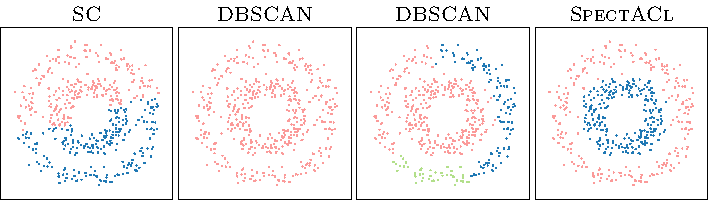
\includegraphics[width=\linewidth]{pics/SAIntroCircles.pdf}
%\documentclass[preview=true]{standalone}
\usepackage{amsmath,amssymb,nicefrac,bbm}
\usepackage{pdfathesis}
\usepackage{etex}
\usepackage{xcolor}
\usepackage[a4paper,left=3.5cm,right=2.5cm,bottom=3.5cm,top=3cm]{geometry}
\usepackage[english]{babel}
\usepackage[round]{natbib}
\usepackage{graphicx,tikz}
\usetikzlibrary{matrix,decorations.pathreplacing, calc, positioning}
\usepackage{relsize} % mathlarger
%\usepackage{hyperref,url}
\usepackage{url}
\usepackage{silence}
\WarningFilter{latex}{Overwriting file}

\usepackage[colorinlistoftodos]{todonotes}
\reversemarginpar
\setlength{\marginparwidth}{3.1cm}
% Theorem-Umgebungen
%\usepackage[amsmath,thmmarks]{ntheorem}
\usepackage{amsthm}
\usepackage{thmtools, thm-restate}
\usepackage{algorithm,algpseudocode}
\algnewcommand{\IIf}[1]{\State\algorithmicif\ #1\ \algorithmicthen}
\algnewcommand{\EndIIf}{\unskip\ \algorithmicend\ \algorithmicif}

\usepackage{enumerate}
\usepackage{booktabs,multirow,adjustbox}
\usepackage[font=small,labelfont=bf]{caption}
\usepackage{subfigure}
\usepackage{pgfplots,filecontents,pgfplotstable}
\usepgfplotslibrary{groupplots}
\pgfplotsset{compat=1.14}
\pgfplotsset{
cohStyle/.style={ctrust,mark options ={ctrust},mark repeat={4}, ultra thick, error bars/.cd,y dir = both, y explicit},
densStyle/.style={cdens,dashed,mark options ={cdens},mark repeat={4}, ultra thick, error bars/.cd,y dir = both, y explicit},
primpStyle/.style={cPrimp,dashed,mark=triangle*,mark options ={cPrimp},mark repeat={3}, ultra thick, error bars/.cd,y dir = both, y explicit},
panStyle/.style={cPan,dashed,mark options ={cPan},mark repeat={3}, ultra thick, error bars/.cd,y dir = both, y explicit},
specStyle/.style={cSpec,mark options ={cSpec},mark repeat={4}, thick, error bars/.cd,y dir = both, y explicit},
specLStyle/.style={cSpecL,mark options ={cSpecL},mark repeat={4}, thick, error bars/.cd,y dir = both, y explicit},
RSCStyle/.style={cRSC,dashed,mark=triangle*,mark options ={cRSC},mark repeat={3}, thick, error bars/.cd,y dir = both, y explicit},
SCStyle/.style={cSC,dashed,mark options ={cSC},mark repeat={3}, thick, error bars/.cd,y dir = both, y explicit},
DBSCANStyle/.style={cDBSCAN,dashed,mark options ={cDBSCAN},mark repeat={3}, thick, error bars/.cd,y dir = both, y explicit},
clusterScatterStyle/.style={scatter/classes={1={cSpecL}, 2={cRSC}, 0={cDBSCAN}, -1={white}},
    scatter, only marks, mark size =0.3, scatter src=explicit symbolic},
nonnegScatterStyle/.style={scatter, only marks, fill=cSpec, scatter src=explicit,
     	visualization depends on ={\thisrow{z} \as \perpointmarksize},
     scatter/@pre marker code/.append style={/tikz/mark size=1.5*\perpointmarksize}},
pandaStyle/.style={cPanda,dashed,mark options ={cPanda},mark repeat={3}, ultra thick, error bars/.cd,y dir = both, y explicit},
punkStyle/.style={cPunk,mark options ={cPunk},mark repeat={3}, thick, error bars/.cd,y dir = both, y explicit},
dbssl1Style/.style={cDBSSL1,dashed,mark options ={cDBSSL1},mark=triangle,mark repeat={3}, thick, error bars/.cd,y dir = both, y explicit},
dbssl2Style/.style={cDBSSL2,dashed,mark options ={cDBSSL2},mark=diamond,mark repeat={3}, thick, error bars/.cd,y dir = both, y explicit},
mdlDbsslStyle/.style={cMDLDBSSL,dashed,mark=star,mark options ={cMDLDBSSL},mark repeat={3}, thick, error bars/.cd,y dir = both, y explicit},
% color change for embedding visualization (fuzzy clusters) 
colormap={test}{[2pt]
    rgb255=(166,206,227);
    rgb255=(166,206,227);
},
}

\Title{ A Mathematical Theory of Making Hard Decisions:
Model Selection and Robustness of Matrix Factorization with Binary
Constraints}

%List of Symbols
\usepackage{nomencl}
\makenomenclature


%\usepackage{color}
\definecolor{col1}{RGB}{166,206,227}
\definecolor{col2}{RGB}{31,120,180}
\definecolor{col3}{RGB}{178,223,138}
\definecolor{col4}{RGB}{51,160,44}
\definecolor{col5}{RGB}{251,154,153}
\definecolor{col6}{RGB}{227,26,28}

\definecolor{cdens}{named}{col1}
\definecolor{ctrust}{named}{col2}
\definecolor{cPrimp}{named}{col3}
\definecolor{cPan}{named}{col4}
\definecolor{cPanda}{named}{col5}
\definecolor{cNassau}{named}{col6}
\definecolor{cMdl4bmf}{named}{col1}


%
\definecolor{cSpec}{named}{col1}
\definecolor{cSpecL}{named}{col2}
\definecolor{cRSC}{named}{col3}
\definecolor{cSC}{named}{col4}
\definecolor{cDBSCAN}{named}{col5}

%
\definecolor{cPunk}{named}{col1}
\definecolor{cDBSSL1}{named}{col2}
\definecolor{cDBSSL2}{named}{col4}
\definecolor{cMDLDBSSL}{named}{col5}
% Theorem-Optionen %
%\theoremseparator{.}
%\newenvironment{proof}{\par\noindent{\textit{ Proof}\ }}{\hfill\qed\\[2mm]}
\theoremstyle{plain}
%\theoremheaderfont{\moon}
%\newcommand{\BlackBox}{\rule{1.5ex}{1.5ex}}  % end of proof
%
\newtheorem{theorem}{Theorem}[chapter]
\newtheorem{corollary}[theorem]{Corollary}
\newtheorem{observation}[theorem]{Observation}
\newtheorem{lemma}[theorem]{Lemma}
%\theorembodyfont{\upshape}
\theoremstyle{definition}
\newtheorem{definition}[theorem]{Definition}
\newtheorem{algSpec}{Algorithm Specification}
\newtheorem*{remark}{Remark}
\newtheorem*{example}{Example}
\newtheorem*{problem}{Problem}

%Operators/Commands
\DeclareMathOperator*{\argmin}{arg\,min}
\DeclareMathOperator*{\argmax}{arg\,max}
\DeclareMathOperator*{\freq}{freq}
\DeclareMathOperator*{\cov}{cov}
\DeclareMathOperator*{\anc}{anc}
\DeclareMathOperator*{\supp}{supp}
\DeclareMathOperator*{\minsup}{minsup}
\DeclareMathOperator*{\tr}{tr}
\DeclareMathOperator*{\bigO}{\mathcal{O}}
\DeclareMathOperator{\diag}{diag}
\DeclareMathOperator{\prox}{prox}
\DeclareMathOperator{\pre}{pre}
\DeclareMathOperator{\rec}{rec}
\newcommand{\Ya}{Y_{\mathcal{J}_a\cdot}}
\newcommand{\Va}{{V_a}}
\newcommand{\Da}{D_{\mathcal{J}_a\cdot}}
\newcommand{\KL}{Kurdyka-{\L}ojasiewicz }
\newcommand{\LXU}{\mathcal{L}}
\newcommand{\F}{\mathcal{F}}
\newcommand{\N}{\mathbb{N}}
\newcommand{\R}{\mathbb{R}}
\newcommand{\estU}{\widetilde{U}_{\widehat{CT}}}
\newcommand{\estu}{\tilde{u}_{\widehat{CT}}}
\newcommand{\estCT}{\widehat{CT}}
\newcommand{\node}{\mathfrak{n}}
\newcommand{\leaf}{\mathfrak{t}}
\newcommand{\krimp}{\textsc{Krimp} }
\newcommand{\shrimp}{\textsc{SHrimp} }
\newcommand{\slim}{\textsc{Slim} }

\makeatletter

\pgfplotstableset{
    zero color/.initial=white,
    zero color/.get=\zerocol,
    zero color/.store in=\zerocol,
    one color/.initial=red,
    one color/.get=\onecol,
    one color/.store in=\onecol,
    color cells/.style={
        every head row/.style={output empty row},
        string type,
        postproc cell content/.code={%
           \pgfkeysalso{@cell content=\rule{0cm}{2.4ex}\cellcolor{\zerocol}
           \pgfmathtruncatemacro\number{int(##1)}
           \ifnum\number>100\cellcolor{\onecol!50!black}
           \else \ifnum\number>0\cellcolor{\onecol!##1}\fi\fi}%
        },
        columns/x/.style={
            column name={},
            postproc cell content/.code={}
        }
    }
}
\makeatother

\makeatletter
\newcommand\footnoteref[1]{\protected@xdef\@thefnmark{\ref{#1}}\@footnotemark}
\makeatother

\makeatletter
%\renewcommand{\@chapapp}{}% Not necessary...
\newenvironment{chapquote}[2][2em]
  {\setlength{\@tempdima}{#1}%
   \def\chapquote@author{#2}%
   \parshape 1 \@tempdima \dimexpr\textwidth-2\@tempdima\relax%
   \itshape}
  {\par\normalfont\hfill--\ \chapquote@author\hspace*{\@tempdima}\par\bigskip}
\makeatother

%Thicker bar
\makeatletter
\newcommand{\thickbar}{\mathpalette\@thickbar}
\newcommand{\@thickbar}[2]{{#1\mkern1.5mu\vbox{
  \sbox\z@{$#1\mkern-1.5mu#2\mkern-1.5mu$}%
  \sbox\tw@{$#1\overline{#2}$}%
  \dimen@=\dimexpr\ht\tw@-\ht\z@-.8\p@\relax
  \hrule\@height.8\p@ % adjust for the desired rule thickness
  \vskip\dimen@
  \box\z@}\mkern1.5mu}
}
\makeatother

%----------box---------------
\usepackage[many]{tcolorbox}
\tcbset{
  myhlight/.style={
    colback=cyan!10,
    arc=0pt,
    outer arc=0pt,
    boxrule=0pt,
    top=2pt,
    bottom=2pt,
    left=2pt,
    right=2pt,
  },
  highlight math style={myhlight},
  mybx/.style={
    colback=white,
    arc=0pt,
    outer arc=0pt,
    boxrule=1pt,
    top=2pt,
    bottom=2pt,
    left=2pt,
    right=2pt,
  }
}

\newtcolorbox{mybox}{
	boxsep=1pt,
  	breakable,
  	mybx
}


% Zeilenabstand einstellen %
\renewcommand{\baselinestretch}{1}
% Floating-Umgebungen anpassen %
\renewcommand{\topfraction}{1.0}
\renewcommand{\bottomfraction}{1.0}
\renewcommand{\floatpagefraction}{1.0}
\renewcommand{\dblfloatpagefraction}{1.0}

% Leere Seite ohne Seitennummer, naechste Seite rechts
\newcommand{\blankpage}{
 \clearpage{\pagestyle{empty}\cleardoublepage}
}

% Keine einzelnen Zeilen beim Anfang eines Abschnitts (Schusterjungen)
\clubpenalty = 10000
% Keine einzelnen Zeilen am Ende eines Abschnitts (Hurenkinder)
\widowpenalty = 10000 \displaywidowpenalty = 10000
% EOF
%
\begin{document}
%
\begin{filecontents}{nmSpectACl_eps.dat}
x y z
1.70069743062 2.42758078324 1
0.285683163483 0.820224134154 1
1.96043338205 1.11652004199 1
2.54379828594 0.801796530514 0
1.02584883691 2.57355440485 1
1.93164886191 1.28604223276 1
1.83409801343 1.05168575212 1
1.50665839702 0.598828682981 0
1.21456049586 1.91816830754 0
0.548489010379 2.4266670795 1
2.43718937566 0.259585631612 0
1.08815940258 1.49111722436 0
1.03453098116 1.5879904518 0
0.109412219779 1.28023561758 1
1.9865620235 1.22135031104 1
1.22512830724 1.0225006133 0
2.86565022133 1.80367677252 0
2.89706812992 1.53195814064 0
0.8209715405 1.72041831352 0
0.617806017378 2.40727584262 1
2.28442347034 0.430331423047 0
1.28180236997 1.03358907376 0
0.887937054635 2.68053646933 1
0.891570602061 2.32922789032 1
2.65618201755 0.894877000626 0
0.498394232883 2.45236217747 1
1.35694280656 2.46718908062 1
1.11489573331 1.85699692515 0
2.9080680088 1.73914577833 0
0.785679177354 2.44215259264 1
0.196823873853 1.89256063131 1
1.17823524744 1.75551785493 0
1.23992030311 2.66315904413 1
2.00540849232 0.499253921452 0
0.848956944163 2.45868527982 1
0.0925078051445 1.29305455349 1
0.247138803261 1.95645113223 1
2.83766305835 1.76420767232 0
1.12807120931 1.38527205119 0
1.94201627226 1.40478582163 1
1.25729757329 1.8930319065 0
1.89326303725 1.91932512895 1
1.72383858092 2.21738324713 1
0.45709546568 2.4199525741 1
1.35307081946 2.21860026432 1
1.00887362506 1.94033464961 0
2.34181723671 0.686515872943 0
1.11475444609 0.954182702693 0
0.420448354856 2.32241979328 1
1.59149868632 2.16078316015 1
0.329310350731 1.82923651818 1
0.629423152641 2.36690609361 1
0.307287028638 1.63670049795 1
2.59724264213 0.569519846613 0
0.527392241622 2.54113453641 1
1.91786921713 0.481595165812 0
1.95156790129 2.12611147089 1
1.41194255779 2.66793976628 1
0.0694222959687 1.82183402009 1
1.61367440743 0.544603242775 0
1.84906416078 1.43524726088 1
2.56840153548 0.978613872479 0
2.68782194498 1.60369331079 0
1.6967066369 2.05018333769 1
0.287779916276 1.35181404437 1
2.10581182305 0.58600544124 0
2.76589189346 1.31793021207 0
0.903330891708 2.71981111471 1
1.78910702143 1.78431684787 1
2.85201486168 1.75683049978 0
2.61444426339 1.1421123448 0
1.76686652891 0.412643118932 0
2.38343223857 0.614019382719 0
0.351982420161 1.82124180438 1
1.20104638372 1.08550087193 0
1.71310358783 2.10563588448 1
1.20574320869 1.14241676927 0
1.85476278831 1.68570217527 1
0.866928473775 2.71912423537 1
1.24150157057 1.87008926301 0
1.28290021851 2.54224942198 1
2.20513157208 0.332694252519 0
0.7649274204 2.49776682771 1
1.92833706433 1.74896192577 1
1.12650480957 1.0348913114 0
0.42035554481 2.29433128095 1
1.8227778128 1.73009804176 1
1.40440087482 0.800372448393 0
0.350170029196 1.83113326458 1
2.67833915261 0.955760684365 0
1.45206309833 2.3376423972 1
1.99881809264 0.647288007188 0
1.73930300342 2.27513141315 1
0.997530664835 2.48601880132 1
2.52748209417 0.964779854994 0
0.18616961175 1.41798846544 1
1.27951506157 0.579681303838 0
1.24451979199 1.01467765734 0
1.528155426 0.429507299506 0
1.86116862662 0.0 0
0.229448043123 1.39451828581 1
2.43840791486 0.811277652094 0
1.08024324217 1.45606914327 0
1.69141952321 1.87996999864 1
0.523342152062 2.27879186696 1
2.53685907702 0.842989476903 0
0.781622595306 2.37059793943 1
2.37151355968 0.752368295204 0
1.81585388656 0.405096626174 0
0.526353426641 2.28139242049 1
2.7760661566 0.95760548246 0
0.923603269543 2.64416122336 1
1.94640723913 1.91848140563 1
1.56063634725 2.50248629435 1
1.0176090148 2.72395908515 1
2.31363407826 0.5281707426 0
1.73803401456 1.88934225142 1
0.26732734312 1.01993624365 1
1.92620482073 1.36669614426 1
2.83528847849 2.08551281403 0
1.2560191234 0.92058406981 0
2.38592708362 0.628151589247 0
1.63132977838 0.709002849989 0
1.05904065429 1.51493849809 0
0.139685121871 1.80990844772 1
1.27499215905 1.06475398303 0
1.14937169414 1.42166121091 0
2.33215946967 0.30036289709 0
1.67510627109 0.411176705111 0
1.18231701939 2.50556350357 1
1.77038669418 1.7965018847 1
2.41711258717 1.06425648687 0
1.5466743199 2.19799847606 1
2.81159915284 0.84108084496 0
2.09568775447 0.361760404015 0
1.62856213766 2.40924498166 1
2.39833092966 0.493171096231 0
1.51465143737 2.47271499647 1
1.13635348992 0.947616890809 0
1.04349043595 1.39023226786 0
0.603031169212 2.58849736575 1
1.9387998979 1.22409851527 1
0.128778294394 1.31392528176 1
1.1003283767 1.2661573588 0
0.743838019158 2.52252993124 1
0.61621116068 2.65631385961 1
0.886728816447 2.57220887 1
1.93703048927 0.497335966775 0
1.34132891502 0.890984584948 0
0.536517048738 2.03140735086 1
0.426818260547 2.19895923382 1
0.382225086449 2.24212488028 1
0.90075749994 2.84889611659 1
1.71053267234 0.139893439754 0
1.29639938455 2.59086974776 1
1.94208010739 0.301786108633 0
1.83766716651 1.89862578133 1
0.217910019358 1.18284981176 1
2.87431916031 1.13362681065 0
2.49128297904 0.808660342234 0
0.887367512053 1.77483826418 0
2.41849255062 0.5324350021 0
1.52025137653 2.40917722219 1
2.81144168216 1.32711652029 0
1.04959124228 1.45154913004 0
2.76797402357 1.57360077806 0
1.82169413997 1.6359444949 1
0.463673012107 2.13666946634 1
1.76717691103 0.185518641762 0
1.79700009392 0.415992627791 0
1.07371926343 1.25433471066 0
0.35340797154 2.20777111939 1
0.910470573245 2.57545855259 1
1.00666113925 1.41487472942 0
0.263242311008 2.11420843779 1
1.83750587555 0.960921001284 1
0.598118607947 2.17126465619 1
0.989607517794 2.72016213659 1
0.339991852275 1.6367039174 1
2.81553150588 1.25227670267 0
1.1688157054 1.61925018628 0
2.87702213607 1.62065697172 0
1.18784418709 1.07176694342 0
2.69535677668 1.14397649917 0
2.61215137255 0.908888019432 0
2.2703000471 0.739737480907 0
0.310292767944 1.5927524401 1
1.9751498572 1.39478059397 1
1.05585797661 1.86898397783 0
0.491864333665 2.31875950071 1
2.04280176433 0.227220807369 0
1.29239733899 2.77729312657 1
1.76399564245 0.389462528366 0
1.10987143975 2.45825835483 1
0.888789567782 2.65387087803 1
2.45980643174 0.992909318285 0
1.08897922761 1.42887358233 0
0.759086710455 2.40740216785 1
2.85579700003 1.62503776295 0
1.49047821489 0.578651837622 0
2.14306688802 0.410252695811 0
2.80690341525 1.04739831031 0
1.08084426927 2.37142988192 1
1.24156411616 1.55517287562 0
1.46082893365 0.841033454439 0
1.13147127699 2.53816467841 1
2.47534170514 0.691577879525 0
0.515186721621 2.37712522384 1
0.738658590011 2.23721041569 1
0.152209727518 1.84671174913 1
2.60849673113 0.841526842613 0
1.04231829692 2.71045161422 1
0.964376417508 1.74174356827 0
0.342359603748 2.31301969708 1
0.312328480287 2.0697583552 1
2.45657728683 0.742808305141 0
1.96519472004 1.95521093343 1
0.976026718348 1.65145435908 0
1.70038574297 0.690680548668 0
1.37321471501 0.593617808351 0
1.34431592493 2.38004670142 1
1.20432098055 1.41547092441 0
1.0929063259 1.64510555084 0
1.14149626236 1.27251025565 0
2.38350457204 0.579440777335 0
1.29738017256 2.28865081481 1
1.19200628952 1.85807567095 0
2.29057019712 0.494581835568 0
1.80036719203 2.25739553896 1
1.7374178378 0.17861431239 0
0.681070242517 2.21529849059 1
1.88653779019 1.71753481275 1
1.66130686 0.453575429025 0
1.05708950661 1.30651646662 0
1.7262189757 2.0892030765 1
1.8743608435 1.34263072606 1
1.48620524338 0.715922906298 0
2.00459538411 0.635140423792 0
0.318587109448 1.92679150556 1
1.37843639956 0.707088283144 0
2.60563623353 0.84239504921 0
2.51013047406 1.15186988552 0
1.09765232658 2.56485848597 1
2.65051441579 0.706858112677 0
0.352710453599 1.60528124984 1
1.367034677 2.342617793 1
2.6778340428 1.27583043688 0
2.77041498717 1.62149290572 0
0.433413700012 2.28661466553 1
2.48279234082 0.838028620621 0
0.664103039947 2.61890924636 1
0.485901366946 2.02729851019 1
1.85342076722 0.311040878791 0
2.24141958751 0.69211889508 0
1.05284501061 0.815302813624 0
1.79533297587 1.72925735288 1
1.59592524946 2.291103752 1
1.12311889981 2.73494294316 1
0.239642607379 1.4708710286 1
2.38074908517 0.178741070048 0
1.95942048639 0.485758418579 0
0.801008762883 2.35832224956 1
1.74336065112 2.52814028379 1
2.00425063315 1.44973882129 1
2.99874263731 1.61490975065 0
1.77010542011 2.37104764753 1
1.512850527 2.28856440723 1
2.45235640311 0.561489373791 0
1.295122251 0.789267498929 0
1.51455075898 0.528202376017 0
0.304527789681 1.21175257382 1
1.21559659311 0.781644945741 0
2.13154242053 0.328030655553 0
1.02901463251 1.60574602789 0
1.04967754137 2.46974317694 1
0.383986869727 1.946959298 1
0.674587230211 2.31409008533 1
2.94816733924 1.82970946363 0
1.46163323762 0.792251773345 0
0.660363196201 2.44792160823 1
2.03001716038 0.213480207542 0
1.36368239515 0.799287249057 0
0.100287359104 1.22065856204 1
2.01060150251 0.464874464476 0
2.02983745816 0.305243543361 0
1.2251556746 1.52746937796 0
2.69691681725 1.71441309537 0
2.85609415251 1.41314756677 0
1.01887468848 2.53297875059 1
1.72087173411 1.97290485697 1
0.0540782987346 1.66034457313 1
1.50772484392 0.172194489983 0
1.24910710679 0.732983283934 0
1.21965279462 1.48366422323 0
1.62105492439 2.04589281976 1
2.87108229353 1.48089493044 0
2.86550061675 1.67997945483 0
1.09627892364 1.65438075877 0
0.338132847221 1.79813179713 1
0.436675834273 2.29829461324 1
1.35612302258 0.617635762047 0
2.71578839431 1.11238360205 0
1.84067753076 2.35076159932 1
1.90883244213 1.40654781879 1
0.448930144962 2.42194163441 1
2.27088828505 0.720328288284 0
1.99427584167 0.292469923157 0
2.05179138307 0.075191975576 0
2.75775762337 1.41657699478 0
0.12405803592 1.67542521447 1
2.43818544068 0.725956693576 0
0.312635410658 1.46319738786 1
0.191240314346 1.65611706549 1
2.75529018146 1.51664712917 0
2.87438941247 1.42513159143 0
1.6124710734 0.108162333984 0
2.07748229347 1.37016700533 1
1.34233953375 0.80510418713 0
0.402666931541 1.97206849653 1
1.59991006122 0.430928345538 0
1.76450324322 1.9417972377 1
0.68142574163 2.3657937995 1
0.164887719809 0.933208295559 1
0.917202040984 2.45367836822 1
0.162413262346 1.79806447542 1
1.69954497521 0.474876958658 0
0.885974873525 2.80037127387 1
1.51432134071 2.26982073221 1
1.34621921819 0.906396320943 0
0.691126264848 2.70915758443 1
1.87293313667 1.78727508456 1
2.28649531765 0.726889577091 0
1.07263048888 2.68627388773 1
1.80060022058 0.599304932113 0
1.26924503947 2.54861366445 1
1.05684697644 1.91308852172 0
1.34125453355 0.95711539541 0
2.8125803328 1.52002754851 0
1.21682707227 0.904424035905 0
1.31929933512 2.79201230232 1
0.637404952623 2.32382669843 1
2.17137726399 0.282323068269 0
1.62762538368 2.26290014007 1
0.540666367159 2.33600275939 1
1.88293690233 1.28480350699 1
2.77912006373 1.9726418669 0
0.887955978785 2.55238946452 1
1.85499981106 2.17561046177 1
2.77275743931 1.26672052764 0
1.88408081212 1.55654855145 1
2.20422656878 0.194151609861 0
1.37215670775 0.64239160578 0
2.74173332893 1.06281332167 0
1.3519692899 2.44789629152 1
0.976624716971 1.76062464088 0
1.04508085459 1.58720561346 0
1.86316148119 0.606405006819 0
1.84838679137 0.364768005124 0
0.3387851597 2.31151471375 1
0.695323634969 2.53219749966 1
1.5016800772 2.28286263615 1
1.72601415658 0.425192245283 0
2.7956168279 1.41300555516 0
0.575132420922 2.21555668975 1
1.92736865662 1.30428244235 1
2.86941042658 1.12652831483 0
0.505972295319 2.11848657916 1
2.88083111935 1.79685857086 0
1.54968608895 2.50447888087 1
2.31278971533 0.259675335988 0
2.73879578515 1.18969715242 0
2.41045930274 0.901294611205 0
0.174601175717 1.25065471515 1
2.32186139204 0.515582850319 0
0.20554231582 1.35225498011 1
2.73059185626 1.20383151563 0
1.3865034904 2.53822490098 1
1.12900900657 2.75114078017 1
0.115069738958 1.04596772082 1
1.335120272 2.64619551797 1
0.831696677651 2.37593629365 1
0.292063587839 1.88454278761 1
1.40477301971 2.48630866567 1
0.227853652523 1.72614884781 1
1.39895080992 2.73195382504 1
2.74706816704 1.76622164219 0
1.65483832512 2.04749839106 1
1.9617597714 0.486798653141 0
1.64888491758 2.17115329123 1
1.60586723589 0.501084875631 0
0.284675287626 1.34679532238 1
1.7675237627 2.24242168385 1
1.26193391783 2.60789114088 1
1.85894079362 1.62496524757 1
1.23674367127 0.982304806675 0
1.97582138089 0.509380358308 0
1.05600781745 2.677392365 1
0.184110621272 2.05447883901 1
0.547385160286 2.55233290655 1
2.57887948172 0.828032733195 0
0.207424483914 1.40821380306 1
1.4369592134 2.72855234245 1
1.62259449811 1.74010086385 1
2.672451501 1.6291678069 0
1.81325243451 0.253878981216 0
1.6389068495 2.55396535903 1
1.78009058629 1.82382255609 1
1.82405310361 2.18872776439 1
0.297924979561 2.15608602252 1
0.734938555418 2.43601614007 1
2.76539867309 0.876829399765 0
0.299689834261 2.26240499707 1
0.657100676443 2.54932984854 1
1.97531757625 0.418517119017 0
1.70335971574 2.01957604536 1
2.01136443846 1.56650446432 1
1.9889246753 1.33708935655 1
0.520697457737 2.19392438309 1
0.201610918869 1.11114702728 1
1.18460310214 2.64018309532 1
1.67953679203 2.09096852593 1
2.52903300028 0.668689176375 0
1.82992609123 0.41148308689 0
1.8782077118 1.15964218423 1
2.77296228387 1.32572928549 0
1.82869717065 0.425653875063 0
0.894053475273 2.44439263156 1
1.07621362954 1.70969278243 0
1.45644007418 2.18215955599 1
1.22063523709 1.744321168 0
1.07967091239 1.06274577676 0
1.1900696085 1.26923933736 0
1.04550909582 1.95159439522 0
1.36599613108 0.996983555907 0
1.48939507438 2.55035208922 1
1.39352940488 0.963024804974 0
1.79847337348 1.76745116277 1
2.79775175948 0.989798501929 0
1.85447215813 0.591984136577 0
1.97133310695 1.23755879013 1
1.33548899995 0.903694832059 0
1.24331015073 2.6153250888 1
1.18889713657 2.78378504495 1
0.959819003516 1.85803345242 0
1.48688739481 0.518828000145 0
2.17038326017 0.538678939108 0
2.00401389267 1.2148267132 1
1.80471537631 1.56843402421 1
2.41227229935 0.418729119508 0
1.54810143205 0.592880123322 0
2.70786075559 1.37847478472 0
1.95754047284 1.18045687789 1
0.376516805236 1.88573157828 1
1.55659448472 1.89138211448 1
1.6713666353 0.452084078249 0
2.01552714856 0.493164592727 0
2.92882892778 1.71535055117 0
2.30685921255 0.69876892802 0
0.910811583335 2.47994266873 1
1.20418470115 2.33843955069 1
2.39790481126 0.794684627456 0
2.46701618738 0.581809838238 0
0.251366988518 1.8780274577 1
0.499412691579 2.38088700981 1
2.56205261531 0.65140655269 0
0.421518010626 2.06060390571 1
1.17009887948 1.5134267149 0
2.81288537691 1.68955621988 0
1.85801783879 0.555828770401 0
1.62002253434 2.06714531107 1
0.587232551254 2.47998567591 1
0.929550119504 2.62696249914 1
0.285941297863 1.76825739547 1
0.259015697972 1.26276981669 1
1.90778512029 1.51870006004 1
1.78857330267 0.328932520462 0
1.62111786442 2.21583017128 1
1.55851506264 2.39564830468 1
2.8184718636 1.49831763883 0
1.44366997728 0.811031572419 0
0.670803912622 2.52569944579 1
1.99900347199 1.27336970112 1
1.03545744455 2.67615661925 1
1.94020677429 0.417071861833 0
1.7209951759 0.415479497045 0
2.44397592822 0.627725787503 0
1.38008876818 0.718105733857 0
2.53036245288 0.380380389259 0
1.95319494442 0.992058285038 1
0.983756955407 1.32684250689 0
0.6881145508 2.71837116248 1
1.88019132883 1.60123260018 1
1.29417582527 1.2231395338 0
1.29745287353 2.79297372882 1
0.333622187036 2.26301752448 1
0.32392659893 1.70725807039 1
1.27163496314 2.5038370693 1
0.419549967659 2.16152124321 1
0.70356632396 2.43698318681 1
2.24311863984 0.0606826745953 0
\end{filecontents}
\begin{filecontents}{nmSpectACl_knn_n.dat}
x y z
1.70069743062 2.42758078324 1
0.285683163483 0.820224134154 1
1.96043338205 1.11652004199 1
2.54379828594 0.801796530514 0
1.02584883691 2.57355440485 1
1.93164886191 1.28604223276 1
1.83409801343 1.05168575212 1
1.50665839702 0.598828682981 0
1.21456049586 1.91816830754 0
0.548489010379 2.4266670795 1
2.43718937566 0.259585631612 0
1.08815940258 1.49111722436 0
1.03453098116 1.5879904518 0
0.109412219779 1.28023561758 1
1.9865620235 1.22135031104 1
1.22512830724 1.0225006133 0
2.86565022133 1.80367677252 0
2.89706812992 1.53195814064 0
0.8209715405 1.72041831352 0
0.617806017378 2.40727584262 1
2.28442347034 0.430331423047 0
1.28180236997 1.03358907376 0
0.887937054635 2.68053646933 1
0.891570602061 2.32922789032 1
2.65618201755 0.894877000626 0
0.498394232883 2.45236217747 1
1.35694280656 2.46718908062 1
1.11489573331 1.85699692515 0
2.9080680088 1.73914577833 0
0.785679177354 2.44215259264 1
0.196823873853 1.89256063131 1
1.17823524744 1.75551785493 0
1.23992030311 2.66315904413 1
2.00540849232 0.499253921452 0
0.848956944163 2.45868527982 1
0.0925078051445 1.29305455349 1
0.247138803261 1.95645113223 1
2.83766305835 1.76420767232 0
1.12807120931 1.38527205119 0
1.94201627226 1.40478582163 1
1.25729757329 1.8930319065 0
1.89326303725 1.91932512895 1
1.72383858092 2.21738324713 1
0.45709546568 2.4199525741 1
1.35307081946 2.21860026432 1
1.00887362506 1.94033464961 0
2.34181723671 0.686515872943 0
1.11475444609 0.954182702693 0
0.420448354856 2.32241979328 1
1.59149868632 2.16078316015 1
0.329310350731 1.82923651818 1
0.629423152641 2.36690609361 1
0.307287028638 1.63670049795 1
2.59724264213 0.569519846613 0
0.527392241622 2.54113453641 1
1.91786921713 0.481595165812 0
1.95156790129 2.12611147089 1
1.41194255779 2.66793976628 1
0.0694222959687 1.82183402009 1
1.61367440743 0.544603242775 0
1.84906416078 1.43524726088 1
2.56840153548 0.978613872479 0
2.68782194498 1.60369331079 0
1.6967066369 2.05018333769 1
0.287779916276 1.35181404437 1
2.10581182305 0.58600544124 0
2.76589189346 1.31793021207 0
0.903330891708 2.71981111471 1
1.78910702143 1.78431684787 1
2.85201486168 1.75683049978 0
2.61444426339 1.1421123448 0
1.76686652891 0.412643118932 0
2.38343223857 0.614019382719 0
0.351982420161 1.82124180438 1
1.20104638372 1.08550087193 0
1.71310358783 2.10563588448 1
1.20574320869 1.14241676927 0
1.85476278831 1.68570217527 1
0.866928473775 2.71912423537 1
1.24150157057 1.87008926301 0
1.28290021851 2.54224942198 1
2.20513157208 0.332694252519 0
0.7649274204 2.49776682771 1
1.92833706433 1.74896192577 1
1.12650480957 1.0348913114 0
0.42035554481 2.29433128095 1
1.8227778128 1.73009804176 1
1.40440087482 0.800372448393 0
0.350170029196 1.83113326458 1
2.67833915261 0.955760684365 0
1.45206309833 2.3376423972 1
1.99881809264 0.647288007188 0
1.73930300342 2.27513141315 1
0.997530664835 2.48601880132 1
2.52748209417 0.964779854994 0
0.18616961175 1.41798846544 1
1.27951506157 0.579681303838 0
1.24451979199 1.01467765734 0
1.528155426 0.429507299506 0
1.86116862662 0.0 0
0.229448043123 1.39451828581 1
2.43840791486 0.811277652094 0
1.08024324217 1.45606914327 0
1.69141952321 1.87996999864 1
0.523342152062 2.27879186696 1
2.53685907702 0.842989476903 0
0.781622595306 2.37059793943 1
2.37151355968 0.752368295204 0
1.81585388656 0.405096626174 0
0.526353426641 2.28139242049 1
2.7760661566 0.95760548246 0
0.923603269543 2.64416122336 1
1.94640723913 1.91848140563 1
1.56063634725 2.50248629435 1
1.0176090148 2.72395908515 1
2.31363407826 0.5281707426 0
1.73803401456 1.88934225142 1
0.26732734312 1.01993624365 1
1.92620482073 1.36669614426 1
2.83528847849 2.08551281403 0
1.2560191234 0.92058406981 0
2.38592708362 0.628151589247 0
1.63132977838 0.709002849989 0
1.05904065429 1.51493849809 0
0.139685121871 1.80990844772 1
1.27499215905 1.06475398303 0
1.14937169414 1.42166121091 0
2.33215946967 0.30036289709 0
1.67510627109 0.411176705111 0
1.18231701939 2.50556350357 1
1.77038669418 1.7965018847 1
2.41711258717 1.06425648687 0
1.5466743199 2.19799847606 1
2.81159915284 0.84108084496 0
2.09568775447 0.361760404015 0
1.62856213766 2.40924498166 1
2.39833092966 0.493171096231 0
1.51465143737 2.47271499647 1
1.13635348992 0.947616890809 0
1.04349043595 1.39023226786 0
0.603031169212 2.58849736575 1
1.9387998979 1.22409851527 1
0.128778294394 1.31392528176 1
1.1003283767 1.2661573588 0
0.743838019158 2.52252993124 1
0.61621116068 2.65631385961 1
0.886728816447 2.57220887 1
1.93703048927 0.497335966775 0
1.34132891502 0.890984584948 0
0.536517048738 2.03140735086 1
0.426818260547 2.19895923382 1
0.382225086449 2.24212488028 1
0.90075749994 2.84889611659 1
1.71053267234 0.139893439754 0
1.29639938455 2.59086974776 1
1.94208010739 0.301786108633 0
1.83766716651 1.89862578133 1
0.217910019358 1.18284981176 1
2.87431916031 1.13362681065 0
2.49128297904 0.808660342234 0
0.887367512053 1.77483826418 0
2.41849255062 0.5324350021 0
1.52025137653 2.40917722219 1
2.81144168216 1.32711652029 0
1.04959124228 1.45154913004 0
2.76797402357 1.57360077806 0
1.82169413997 1.6359444949 1
0.463673012107 2.13666946634 1
1.76717691103 0.185518641762 0
1.79700009392 0.415992627791 0
1.07371926343 1.25433471066 0
0.35340797154 2.20777111939 1
0.910470573245 2.57545855259 1
1.00666113925 1.41487472942 0
0.263242311008 2.11420843779 1
1.83750587555 0.960921001284 1
0.598118607947 2.17126465619 1
0.989607517794 2.72016213659 1
0.339991852275 1.6367039174 1
2.81553150588 1.25227670267 0
1.1688157054 1.61925018628 0
2.87702213607 1.62065697172 0
1.18784418709 1.07176694342 0
2.69535677668 1.14397649917 0
2.61215137255 0.908888019432 0
2.2703000471 0.739737480907 0
0.310292767944 1.5927524401 1
1.9751498572 1.39478059397 1
1.05585797661 1.86898397783 0
0.491864333665 2.31875950071 1
2.04280176433 0.227220807369 0
1.29239733899 2.77729312657 1
1.76399564245 0.389462528366 0
1.10987143975 2.45825835483 1
0.888789567782 2.65387087803 1
2.45980643174 0.992909318285 0
1.08897922761 1.42887358233 0
0.759086710455 2.40740216785 1
2.85579700003 1.62503776295 0
1.49047821489 0.578651837622 0
2.14306688802 0.410252695811 0
2.80690341525 1.04739831031 0
1.08084426927 2.37142988192 1
1.24156411616 1.55517287562 0
1.46082893365 0.841033454439 0
1.13147127699 2.53816467841 1
2.47534170514 0.691577879525 0
0.515186721621 2.37712522384 1
0.738658590011 2.23721041569 1
0.152209727518 1.84671174913 1
2.60849673113 0.841526842613 0
1.04231829692 2.71045161422 1
0.964376417508 1.74174356827 0
0.342359603748 2.31301969708 1
0.312328480287 2.0697583552 1
2.45657728683 0.742808305141 0
1.96519472004 1.95521093343 1
0.976026718348 1.65145435908 0
1.70038574297 0.690680548668 0
1.37321471501 0.593617808351 0
1.34431592493 2.38004670142 1
1.20432098055 1.41547092441 0
1.0929063259 1.64510555084 0
1.14149626236 1.27251025565 0
2.38350457204 0.579440777335 0
1.29738017256 2.28865081481 1
1.19200628952 1.85807567095 0
2.29057019712 0.494581835568 0
1.80036719203 2.25739553896 1
1.7374178378 0.17861431239 0
0.681070242517 2.21529849059 1
1.88653779019 1.71753481275 1
1.66130686 0.453575429025 0
1.05708950661 1.30651646662 0
1.7262189757 2.0892030765 1
1.8743608435 1.34263072606 1
1.48620524338 0.715922906298 0
2.00459538411 0.635140423792 0
0.318587109448 1.92679150556 1
1.37843639956 0.707088283144 0
2.60563623353 0.84239504921 0
2.51013047406 1.15186988552 0
1.09765232658 2.56485848597 1
2.65051441579 0.706858112677 0
0.352710453599 1.60528124984 1
1.367034677 2.342617793 1
2.6778340428 1.27583043688 0
2.77041498717 1.62149290572 0
0.433413700012 2.28661466553 1
2.48279234082 0.838028620621 0
0.664103039947 2.61890924636 1
0.485901366946 2.02729851019 1
1.85342076722 0.311040878791 0
2.24141958751 0.69211889508 0
1.05284501061 0.815302813624 0
1.79533297587 1.72925735288 1
1.59592524946 2.291103752 1
1.12311889981 2.73494294316 1
0.239642607379 1.4708710286 1
2.38074908517 0.178741070048 0
1.95942048639 0.485758418579 0
0.801008762883 2.35832224956 1
1.74336065112 2.52814028379 1
2.00425063315 1.44973882129 1
2.99874263731 1.61490975065 0
1.77010542011 2.37104764753 1
1.512850527 2.28856440723 1
2.45235640311 0.561489373791 0
1.295122251 0.789267498929 0
1.51455075898 0.528202376017 0
0.304527789681 1.21175257382 1
1.21559659311 0.781644945741 0
2.13154242053 0.328030655553 0
1.02901463251 1.60574602789 0
1.04967754137 2.46974317694 1
0.383986869727 1.946959298 1
0.674587230211 2.31409008533 1
2.94816733924 1.82970946363 0
1.46163323762 0.792251773345 0
0.660363196201 2.44792160823 1
2.03001716038 0.213480207542 0
1.36368239515 0.799287249057 0
0.100287359104 1.22065856204 1
2.01060150251 0.464874464476 0
2.02983745816 0.305243543361 0
1.2251556746 1.52746937796 0
2.69691681725 1.71441309537 0
2.85609415251 1.41314756677 0
1.01887468848 2.53297875059 1
1.72087173411 1.97290485697 1
0.0540782987346 1.66034457313 1
1.50772484392 0.172194489983 0
1.24910710679 0.732983283934 0
1.21965279462 1.48366422323 0
1.62105492439 2.04589281976 1
2.87108229353 1.48089493044 0
2.86550061675 1.67997945483 0
1.09627892364 1.65438075877 0
0.338132847221 1.79813179713 1
0.436675834273 2.29829461324 1
1.35612302258 0.617635762047 0
2.71578839431 1.11238360205 0
1.84067753076 2.35076159932 1
1.90883244213 1.40654781879 1
0.448930144962 2.42194163441 1
2.27088828505 0.720328288284 0
1.99427584167 0.292469923157 0
2.05179138307 0.075191975576 0
2.75775762337 1.41657699478 0
0.12405803592 1.67542521447 1
2.43818544068 0.725956693576 0
0.312635410658 1.46319738786 1
0.191240314346 1.65611706549 1
2.75529018146 1.51664712917 0
2.87438941247 1.42513159143 0
1.6124710734 0.108162333984 0
2.07748229347 1.37016700533 1
1.34233953375 0.80510418713 0
0.402666931541 1.97206849653 1
1.59991006122 0.430928345538 0
1.76450324322 1.9417972377 1
0.68142574163 2.3657937995 1
0.164887719809 0.933208295559 1
0.917202040984 2.45367836822 1
0.162413262346 1.79806447542 1
1.69954497521 0.474876958658 0
0.885974873525 2.80037127387 1
1.51432134071 2.26982073221 1
1.34621921819 0.906396320943 0
0.691126264848 2.70915758443 1
1.87293313667 1.78727508456 1
2.28649531765 0.726889577091 0
1.07263048888 2.68627388773 1
1.80060022058 0.599304932113 0
1.26924503947 2.54861366445 1
1.05684697644 1.91308852172 0
1.34125453355 0.95711539541 0
2.8125803328 1.52002754851 0
1.21682707227 0.904424035905 0
1.31929933512 2.79201230232 1
0.637404952623 2.32382669843 1
2.17137726399 0.282323068269 0
1.62762538368 2.26290014007 1
0.540666367159 2.33600275939 1
1.88293690233 1.28480350699 1
2.77912006373 1.9726418669 0
0.887955978785 2.55238946452 1
1.85499981106 2.17561046177 1
2.77275743931 1.26672052764 0
1.88408081212 1.55654855145 1
2.20422656878 0.194151609861 0
1.37215670775 0.64239160578 0
2.74173332893 1.06281332167 0
1.3519692899 2.44789629152 1
0.976624716971 1.76062464088 0
1.04508085459 1.58720561346 0
1.86316148119 0.606405006819 0
1.84838679137 0.364768005124 0
0.3387851597 2.31151471375 1
0.695323634969 2.53219749966 1
1.5016800772 2.28286263615 1
1.72601415658 0.425192245283 0
2.7956168279 1.41300555516 0
0.575132420922 2.21555668975 1
1.92736865662 1.30428244235 1
2.86941042658 1.12652831483 0
0.505972295319 2.11848657916 1
2.88083111935 1.79685857086 0
1.54968608895 2.50447888087 1
2.31278971533 0.259675335988 0
2.73879578515 1.18969715242 0
2.41045930274 0.901294611205 0
0.174601175717 1.25065471515 1
2.32186139204 0.515582850319 0
0.20554231582 1.35225498011 1
2.73059185626 1.20383151563 0
1.3865034904 2.53822490098 1
1.12900900657 2.75114078017 1
0.115069738958 1.04596772082 1
1.335120272 2.64619551797 1
0.831696677651 2.37593629365 1
0.292063587839 1.88454278761 1
1.40477301971 2.48630866567 1
0.227853652523 1.72614884781 1
1.39895080992 2.73195382504 1
2.74706816704 1.76622164219 0
1.65483832512 2.04749839106 1
1.9617597714 0.486798653141 0
1.64888491758 2.17115329123 1
1.60586723589 0.501084875631 0
0.284675287626 1.34679532238 1
1.7675237627 2.24242168385 1
1.26193391783 2.60789114088 1
1.85894079362 1.62496524757 1
1.23674367127 0.982304806675 0
1.97582138089 0.509380358308 0
1.05600781745 2.677392365 1
0.184110621272 2.05447883901 1
0.547385160286 2.55233290655 1
2.57887948172 0.828032733195 0
0.207424483914 1.40821380306 1
1.4369592134 2.72855234245 1
1.62259449811 1.74010086385 1
2.672451501 1.6291678069 0
1.81325243451 0.253878981216 0
1.6389068495 2.55396535903 1
1.78009058629 1.82382255609 1
1.82405310361 2.18872776439 1
0.297924979561 2.15608602252 1
0.734938555418 2.43601614007 1
2.76539867309 0.876829399765 0
0.299689834261 2.26240499707 1
0.657100676443 2.54932984854 1
1.97531757625 0.418517119017 0
1.70335971574 2.01957604536 1
2.01136443846 1.56650446432 1
1.9889246753 1.33708935655 1
0.520697457737 2.19392438309 1
0.201610918869 1.11114702728 1
1.18460310214 2.64018309532 1
1.67953679203 2.09096852593 1
2.52903300028 0.668689176375 0
1.82992609123 0.41148308689 0
1.8782077118 1.15964218423 1
2.77296228387 1.32572928549 0
1.82869717065 0.425653875063 0
0.894053475273 2.44439263156 1
1.07621362954 1.70969278243 0
1.45644007418 2.18215955599 1
1.22063523709 1.744321168 0
1.07967091239 1.06274577676 0
1.1900696085 1.26923933736 0
1.04550909582 1.95159439522 0
1.36599613108 0.996983555907 0
1.48939507438 2.55035208922 1
1.39352940488 0.963024804974 0
1.79847337348 1.76745116277 1
2.79775175948 0.989798501929 0
1.85447215813 0.591984136577 0
1.97133310695 1.23755879013 1
1.33548899995 0.903694832059 0
1.24331015073 2.6153250888 1
1.18889713657 2.78378504495 1
0.959819003516 1.85803345242 0
1.48688739481 0.518828000145 0
2.17038326017 0.538678939108 0
2.00401389267 1.2148267132 1
1.80471537631 1.56843402421 1
2.41227229935 0.418729119508 0
1.54810143205 0.592880123322 0
2.70786075559 1.37847478472 0
1.95754047284 1.18045687789 1
0.376516805236 1.88573157828 1
1.55659448472 1.89138211448 1
1.6713666353 0.452084078249 0
2.01552714856 0.493164592727 0
2.92882892778 1.71535055117 0
2.30685921255 0.69876892802 0
0.910811583335 2.47994266873 1
1.20418470115 2.33843955069 1
2.39790481126 0.794684627456 0
2.46701618738 0.581809838238 0
0.251366988518 1.8780274577 1
0.499412691579 2.38088700981 1
2.56205261531 0.65140655269 0
0.421518010626 2.06060390571 1
1.17009887948 1.5134267149 0
2.81288537691 1.68955621988 0
1.85801783879 0.555828770401 0
1.62002253434 2.06714531107 1
0.587232551254 2.47998567591 1
0.929550119504 2.62696249914 1
0.285941297863 1.76825739547 1
0.259015697972 1.26276981669 1
1.90778512029 1.51870006004 1
1.78857330267 0.328932520462 0
1.62111786442 2.21583017128 1
1.55851506264 2.39564830468 1
2.8184718636 1.49831763883 0
1.44366997728 0.811031572419 0
0.670803912622 2.52569944579 1
1.99900347199 1.27336970112 1
1.03545744455 2.67615661925 1
1.94020677429 0.417071861833 0
1.7209951759 0.415479497045 0
2.44397592822 0.627725787503 0
1.38008876818 0.718105733857 0
2.53036245288 0.380380389259 0
1.95319494442 0.992058285038 1
0.983756955407 1.32684250689 0
0.6881145508 2.71837116248 1
1.88019132883 1.60123260018 1
1.29417582527 1.2231395338 0
1.29745287353 2.79297372882 1
0.333622187036 2.26301752448 1
0.32392659893 1.70725807039 1
1.27163496314 2.5038370693 1
0.419549967659 2.16152124321 1
0.70356632396 2.43698318681 1
2.24311863984 0.0606826745953 0
\end{filecontents}
\begin{filecontents}{nmSC_knn_n.dat}
x y z
1.70069743062 2.42758078324 0
0.285683163483 0.820224134154 0
1.96043338205 1.11652004199 1
2.54379828594 0.801796530514 1
1.02584883691 2.57355440485 0
1.93164886191 1.28604223276 1
1.83409801343 1.05168575212 1
1.50665839702 0.598828682981 1
1.21456049586 1.91816830754 1
0.548489010379 2.4266670795 0
2.43718937566 0.259585631612 1
1.08815940258 1.49111722436 1
1.03453098116 1.5879904518 1
0.109412219779 1.28023561758 0
1.9865620235 1.22135031104 1
1.22512830724 1.0225006133 1
2.86565022133 1.80367677252 1
2.89706812992 1.53195814064 1
0.8209715405 1.72041831352 1
0.617806017378 2.40727584262 0
2.28442347034 0.430331423047 1
1.28180236997 1.03358907376 1
0.887937054635 2.68053646933 0
0.891570602061 2.32922789032 0
2.65618201755 0.894877000626 1
0.498394232883 2.45236217747 0
1.35694280656 2.46718908062 0
1.11489573331 1.85699692515 1
2.9080680088 1.73914577833 1
0.785679177354 2.44215259264 0
0.196823873853 1.89256063131 0
1.17823524744 1.75551785493 1
1.23992030311 2.66315904413 0
2.00540849232 0.499253921452 1
0.848956944163 2.45868527982 0
0.0925078051445 1.29305455349 0
0.247138803261 1.95645113223 0
2.83766305835 1.76420767232 1
1.12807120931 1.38527205119 1
1.94201627226 1.40478582163 1
1.25729757329 1.8930319065 1
1.89326303725 1.91932512895 0
1.72383858092 2.21738324713 0
0.45709546568 2.4199525741 0
1.35307081946 2.21860026432 0
1.00887362506 1.94033464961 1
2.34181723671 0.686515872943 1
1.11475444609 0.954182702693 1
0.420448354856 2.32241979328 0
1.59149868632 2.16078316015 0
0.329310350731 1.82923651818 0
0.629423152641 2.36690609361 0
0.307287028638 1.63670049795 0
2.59724264213 0.569519846613 1
0.527392241622 2.54113453641 0
1.91786921713 0.481595165812 1
1.95156790129 2.12611147089 0
1.41194255779 2.66793976628 0
0.0694222959687 1.82183402009 0
1.61367440743 0.544603242775 1
1.84906416078 1.43524726088 1
2.56840153548 0.978613872479 1
2.68782194498 1.60369331079 1
1.6967066369 2.05018333769 0
0.287779916276 1.35181404437 0
2.10581182305 0.58600544124 1
2.76589189346 1.31793021207 1
0.903330891708 2.71981111471 0
1.78910702143 1.78431684787 0
2.85201486168 1.75683049978 1
2.61444426339 1.1421123448 1
1.76686652891 0.412643118932 1
2.38343223857 0.614019382719 1
0.351982420161 1.82124180438 0
1.20104638372 1.08550087193 1
1.71310358783 2.10563588448 0
1.20574320869 1.14241676927 1
1.85476278831 1.68570217527 1
0.866928473775 2.71912423537 0
1.24150157057 1.87008926301 1
1.28290021851 2.54224942198 0
2.20513157208 0.332694252519 1
0.7649274204 2.49776682771 0
1.92833706433 1.74896192577 0
1.12650480957 1.0348913114 1
0.42035554481 2.29433128095 0
1.8227778128 1.73009804176 0
1.40440087482 0.800372448393 1
0.350170029196 1.83113326458 0
2.67833915261 0.955760684365 1
1.45206309833 2.3376423972 0
1.99881809264 0.647288007188 1
1.73930300342 2.27513141315 0
0.997530664835 2.48601880132 0
2.52748209417 0.964779854994 1
0.18616961175 1.41798846544 0
1.27951506157 0.579681303838 1
1.24451979199 1.01467765734 1
1.528155426 0.429507299506 1
1.86116862662 0.0 1
0.229448043123 1.39451828581 0
2.43840791486 0.811277652094 1
1.08024324217 1.45606914327 1
1.69141952321 1.87996999864 0
0.523342152062 2.27879186696 0
2.53685907702 0.842989476903 1
0.781622595306 2.37059793943 0
2.37151355968 0.752368295204 1
1.81585388656 0.405096626174 1
0.526353426641 2.28139242049 0
2.7760661566 0.95760548246 1
0.923603269543 2.64416122336 0
1.94640723913 1.91848140563 0
1.56063634725 2.50248629435 0
1.0176090148 2.72395908515 0
2.31363407826 0.5281707426 1
1.73803401456 1.88934225142 0
0.26732734312 1.01993624365 0
1.92620482073 1.36669614426 1
2.83528847849 2.08551281403 1
1.2560191234 0.92058406981 1
2.38592708362 0.628151589247 1
1.63132977838 0.709002849989 1
1.05904065429 1.51493849809 1
0.139685121871 1.80990844772 0
1.27499215905 1.06475398303 1
1.14937169414 1.42166121091 1
2.33215946967 0.30036289709 1
1.67510627109 0.411176705111 1
1.18231701939 2.50556350357 0
1.77038669418 1.7965018847 0
2.41711258717 1.06425648687 1
1.5466743199 2.19799847606 0
2.81159915284 0.84108084496 1
2.09568775447 0.361760404015 1
1.62856213766 2.40924498166 0
2.39833092966 0.493171096231 1
1.51465143737 2.47271499647 0
1.13635348992 0.947616890809 1
1.04349043595 1.39023226786 1
0.603031169212 2.58849736575 0
1.9387998979 1.22409851527 1
0.128778294394 1.31392528176 0
1.1003283767 1.2661573588 1
0.743838019158 2.52252993124 0
0.61621116068 2.65631385961 0
0.886728816447 2.57220887 0
1.93703048927 0.497335966775 1
1.34132891502 0.890984584948 1
0.536517048738 2.03140735086 0
0.426818260547 2.19895923382 0
0.382225086449 2.24212488028 0
0.90075749994 2.84889611659 0
1.71053267234 0.139893439754 1
1.29639938455 2.59086974776 0
1.94208010739 0.301786108633 1
1.83766716651 1.89862578133 0
0.217910019358 1.18284981176 0
2.87431916031 1.13362681065 1
2.49128297904 0.808660342234 1
0.887367512053 1.77483826418 1
2.41849255062 0.5324350021 1
1.52025137653 2.40917722219 0
2.81144168216 1.32711652029 1
1.04959124228 1.45154913004 1
2.76797402357 1.57360077806 1
1.82169413997 1.6359444949 1
0.463673012107 2.13666946634 0
1.76717691103 0.185518641762 1
1.79700009392 0.415992627791 1
1.07371926343 1.25433471066 1
0.35340797154 2.20777111939 0
0.910470573245 2.57545855259 0
1.00666113925 1.41487472942 1
0.263242311008 2.11420843779 0
1.83750587555 0.960921001284 1
0.598118607947 2.17126465619 0
0.989607517794 2.72016213659 0
0.339991852275 1.6367039174 0
2.81553150588 1.25227670267 1
1.1688157054 1.61925018628 1
2.87702213607 1.62065697172 1
1.18784418709 1.07176694342 1
2.69535677668 1.14397649917 1
2.61215137255 0.908888019432 1
2.2703000471 0.739737480907 1
0.310292767944 1.5927524401 0
1.9751498572 1.39478059397 1
1.05585797661 1.86898397783 1
0.491864333665 2.31875950071 0
2.04280176433 0.227220807369 1
1.29239733899 2.77729312657 0
1.76399564245 0.389462528366 1
1.10987143975 2.45825835483 0
0.888789567782 2.65387087803 0
2.45980643174 0.992909318285 1
1.08897922761 1.42887358233 1
0.759086710455 2.40740216785 0
2.85579700003 1.62503776295 1
1.49047821489 0.578651837622 1
2.14306688802 0.410252695811 1
2.80690341525 1.04739831031 1
1.08084426927 2.37142988192 0
1.24156411616 1.55517287562 1
1.46082893365 0.841033454439 1
1.13147127699 2.53816467841 0
2.47534170514 0.691577879525 1
0.515186721621 2.37712522384 0
0.738658590011 2.23721041569 0
0.152209727518 1.84671174913 0
2.60849673113 0.841526842613 1
1.04231829692 2.71045161422 0
0.964376417508 1.74174356827 1
0.342359603748 2.31301969708 0
0.312328480287 2.0697583552 0
2.45657728683 0.742808305141 1
1.96519472004 1.95521093343 0
0.976026718348 1.65145435908 1
1.70038574297 0.690680548668 1
1.37321471501 0.593617808351 1
1.34431592493 2.38004670142 0
1.20432098055 1.41547092441 1
1.0929063259 1.64510555084 1
1.14149626236 1.27251025565 1
2.38350457204 0.579440777335 1
1.29738017256 2.28865081481 0
1.19200628952 1.85807567095 1
2.29057019712 0.494581835568 1
1.80036719203 2.25739553896 0
1.7374178378 0.17861431239 1
0.681070242517 2.21529849059 0
1.88653779019 1.71753481275 0
1.66130686 0.453575429025 1
1.05708950661 1.30651646662 1
1.7262189757 2.0892030765 0
1.8743608435 1.34263072606 1
1.48620524338 0.715922906298 1
2.00459538411 0.635140423792 1
0.318587109448 1.92679150556 0
1.37843639956 0.707088283144 1
2.60563623353 0.84239504921 1
2.51013047406 1.15186988552 1
1.09765232658 2.56485848597 0
2.65051441579 0.706858112677 1
0.352710453599 1.60528124984 0
1.367034677 2.342617793 0
2.6778340428 1.27583043688 1
2.77041498717 1.62149290572 1
0.433413700012 2.28661466553 0
2.48279234082 0.838028620621 1
0.664103039947 2.61890924636 0
0.485901366946 2.02729851019 0
1.85342076722 0.311040878791 1
2.24141958751 0.69211889508 1
1.05284501061 0.815302813624 1
1.79533297587 1.72925735288 0
1.59592524946 2.291103752 0
1.12311889981 2.73494294316 0
0.239642607379 1.4708710286 0
2.38074908517 0.178741070048 1
1.95942048639 0.485758418579 1
0.801008762883 2.35832224956 0
1.74336065112 2.52814028379 0
2.00425063315 1.44973882129 1
2.99874263731 1.61490975065 1
1.77010542011 2.37104764753 0
1.512850527 2.28856440723 0
2.45235640311 0.561489373791 1
1.295122251 0.789267498929 1
1.51455075898 0.528202376017 1
0.304527789681 1.21175257382 0
1.21559659311 0.781644945741 1
2.13154242053 0.328030655553 1
1.02901463251 1.60574602789 1
1.04967754137 2.46974317694 0
0.383986869727 1.946959298 0
0.674587230211 2.31409008533 0
2.94816733924 1.82970946363 1
1.46163323762 0.792251773345 1
0.660363196201 2.44792160823 0
2.03001716038 0.213480207542 1
1.36368239515 0.799287249057 1
0.100287359104 1.22065856204 0
2.01060150251 0.464874464476 1
2.02983745816 0.305243543361 1
1.2251556746 1.52746937796 1
2.69691681725 1.71441309537 1
2.85609415251 1.41314756677 1
1.01887468848 2.53297875059 0
1.72087173411 1.97290485697 0
0.0540782987346 1.66034457313 0
1.50772484392 0.172194489983 1
1.24910710679 0.732983283934 1
1.21965279462 1.48366422323 1
1.62105492439 2.04589281976 0
2.87108229353 1.48089493044 1
2.86550061675 1.67997945483 1
1.09627892364 1.65438075877 1
0.338132847221 1.79813179713 0
0.436675834273 2.29829461324 0
1.35612302258 0.617635762047 1
2.71578839431 1.11238360205 1
1.84067753076 2.35076159932 0
1.90883244213 1.40654781879 1
0.448930144962 2.42194163441 0
2.27088828505 0.720328288284 1
1.99427584167 0.292469923157 1
2.05179138307 0.075191975576 1
2.75775762337 1.41657699478 1
0.12405803592 1.67542521447 0
2.43818544068 0.725956693576 1
0.312635410658 1.46319738786 0
0.191240314346 1.65611706549 0
2.75529018146 1.51664712917 1
2.87438941247 1.42513159143 1
1.6124710734 0.108162333984 1
2.07748229347 1.37016700533 1
1.34233953375 0.80510418713 1
0.402666931541 1.97206849653 0
1.59991006122 0.430928345538 1
1.76450324322 1.9417972377 0
0.68142574163 2.3657937995 0
0.164887719809 0.933208295559 0
0.917202040984 2.45367836822 0
0.162413262346 1.79806447542 0
1.69954497521 0.474876958658 1
0.885974873525 2.80037127387 0
1.51432134071 2.26982073221 0
1.34621921819 0.906396320943 1
0.691126264848 2.70915758443 0
1.87293313667 1.78727508456 0
2.28649531765 0.726889577091 1
1.07263048888 2.68627388773 0
1.80060022058 0.599304932113 1
1.26924503947 2.54861366445 0
1.05684697644 1.91308852172 1
1.34125453355 0.95711539541 1
2.8125803328 1.52002754851 1
1.21682707227 0.904424035905 1
1.31929933512 2.79201230232 0
0.637404952623 2.32382669843 0
2.17137726399 0.282323068269 1
1.62762538368 2.26290014007 0
0.540666367159 2.33600275939 0
1.88293690233 1.28480350699 1
2.77912006373 1.9726418669 1
0.887955978785 2.55238946452 0
1.85499981106 2.17561046177 0
2.77275743931 1.26672052764 1
1.88408081212 1.55654855145 1
2.20422656878 0.194151609861 1
1.37215670775 0.64239160578 1
2.74173332893 1.06281332167 1
1.3519692899 2.44789629152 0
0.976624716971 1.76062464088 1
1.04508085459 1.58720561346 1
1.86316148119 0.606405006819 1
1.84838679137 0.364768005124 1
0.3387851597 2.31151471375 0
0.695323634969 2.53219749966 0
1.5016800772 2.28286263615 0
1.72601415658 0.425192245283 1
2.7956168279 1.41300555516 1
0.575132420922 2.21555668975 0
1.92736865662 1.30428244235 1
2.86941042658 1.12652831483 1
0.505972295319 2.11848657916 0
2.88083111935 1.79685857086 1
1.54968608895 2.50447888087 0
2.31278971533 0.259675335988 1
2.73879578515 1.18969715242 1
2.41045930274 0.901294611205 1
0.174601175717 1.25065471515 0
2.32186139204 0.515582850319 1
0.20554231582 1.35225498011 0
2.73059185626 1.20383151563 1
1.3865034904 2.53822490098 0
1.12900900657 2.75114078017 0
0.115069738958 1.04596772082 0
1.335120272 2.64619551797 0
0.831696677651 2.37593629365 0
0.292063587839 1.88454278761 0
1.40477301971 2.48630866567 0
0.227853652523 1.72614884781 0
1.39895080992 2.73195382504 0
2.74706816704 1.76622164219 1
1.65483832512 2.04749839106 0
1.9617597714 0.486798653141 1
1.64888491758 2.17115329123 0
1.60586723589 0.501084875631 1
0.284675287626 1.34679532238 0
1.7675237627 2.24242168385 0
1.26193391783 2.60789114088 0
1.85894079362 1.62496524757 1
1.23674367127 0.982304806675 1
1.97582138089 0.509380358308 1
1.05600781745 2.677392365 0
0.184110621272 2.05447883901 0
0.547385160286 2.55233290655 0
2.57887948172 0.828032733195 1
0.207424483914 1.40821380306 0
1.4369592134 2.72855234245 0
1.62259449811 1.74010086385 0
2.672451501 1.6291678069 1
1.81325243451 0.253878981216 1
1.6389068495 2.55396535903 0
1.78009058629 1.82382255609 0
1.82405310361 2.18872776439 0
0.297924979561 2.15608602252 0
0.734938555418 2.43601614007 0
2.76539867309 0.876829399765 1
0.299689834261 2.26240499707 0
0.657100676443 2.54932984854 0
1.97531757625 0.418517119017 1
1.70335971574 2.01957604536 0
2.01136443846 1.56650446432 1
1.9889246753 1.33708935655 1
0.520697457737 2.19392438309 0
0.201610918869 1.11114702728 0
1.18460310214 2.64018309532 0
1.67953679203 2.09096852593 0
2.52903300028 0.668689176375 1
1.82992609123 0.41148308689 1
1.8782077118 1.15964218423 1
2.77296228387 1.32572928549 1
1.82869717065 0.425653875063 1
0.894053475273 2.44439263156 0
1.07621362954 1.70969278243 1
1.45644007418 2.18215955599 0
1.22063523709 1.744321168 1
1.07967091239 1.06274577676 1
1.1900696085 1.26923933736 1
1.04550909582 1.95159439522 1
1.36599613108 0.996983555907 1
1.48939507438 2.55035208922 0
1.39352940488 0.963024804974 1
1.79847337348 1.76745116277 0
2.79775175948 0.989798501929 1
1.85447215813 0.591984136577 1
1.97133310695 1.23755879013 1
1.33548899995 0.903694832059 1
1.24331015073 2.6153250888 0
1.18889713657 2.78378504495 0
0.959819003516 1.85803345242 1
1.48688739481 0.518828000145 1
2.17038326017 0.538678939108 1
2.00401389267 1.2148267132 1
1.80471537631 1.56843402421 1
2.41227229935 0.418729119508 1
1.54810143205 0.592880123322 1
2.70786075559 1.37847478472 1
1.95754047284 1.18045687789 1
0.376516805236 1.88573157828 0
1.55659448472 1.89138211448 0
1.6713666353 0.452084078249 1
2.01552714856 0.493164592727 1
2.92882892778 1.71535055117 1
2.30685921255 0.69876892802 1
0.910811583335 2.47994266873 0
1.20418470115 2.33843955069 0
2.39790481126 0.794684627456 1
2.46701618738 0.581809838238 1
0.251366988518 1.8780274577 0
0.499412691579 2.38088700981 0
2.56205261531 0.65140655269 1
0.421518010626 2.06060390571 0
1.17009887948 1.5134267149 1
2.81288537691 1.68955621988 1
1.85801783879 0.555828770401 1
1.62002253434 2.06714531107 0
0.587232551254 2.47998567591 0
0.929550119504 2.62696249914 0
0.285941297863 1.76825739547 0
0.259015697972 1.26276981669 0
1.90778512029 1.51870006004 1
1.78857330267 0.328932520462 1
1.62111786442 2.21583017128 0
1.55851506264 2.39564830468 0
2.8184718636 1.49831763883 1
1.44366997728 0.811031572419 1
0.670803912622 2.52569944579 0
1.99900347199 1.27336970112 1
1.03545744455 2.67615661925 0
1.94020677429 0.417071861833 1
1.7209951759 0.415479497045 1
2.44397592822 0.627725787503 1
1.38008876818 0.718105733857 1
2.53036245288 0.380380389259 1
1.95319494442 0.992058285038 1
0.983756955407 1.32684250689 1
0.6881145508 2.71837116248 0
1.88019132883 1.60123260018 1
1.29417582527 1.2231395338 1
1.29745287353 2.79297372882 0
0.333622187036 2.26301752448 0
0.32392659893 1.70725807039 0
1.27163496314 2.5038370693 0
0.419549967659 2.16152124321 0
0.70356632396 2.43698318681 0
2.24311863984 0.0606826745953 1
\end{filecontents}
\begin{filecontents}{nmRSC.dat}
x y z
1.70069743062 2.42758078324 1
0.285683163483 0.820224134154 1
1.96043338205 1.11652004199 1
2.54379828594 0.801796530514 0
1.02584883691 2.57355440485 1
1.93164886191 1.28604223276 1
1.83409801343 1.05168575212 1
1.50665839702 0.598828682981 0
1.21456049586 1.91816830754 0
0.548489010379 2.4266670795 1
2.43718937566 0.259585631612 0
1.08815940258 1.49111722436 0
1.03453098116 1.5879904518 0
0.109412219779 1.28023561758 1
1.9865620235 1.22135031104 1
1.22512830724 1.0225006133 0
2.86565022133 1.80367677252 0
2.89706812992 1.53195814064 0
0.8209715405 1.72041831352 0
0.617806017378 2.40727584262 1
2.28442347034 0.430331423047 0
1.28180236997 1.03358907376 0
0.887937054635 2.68053646933 1
0.891570602061 2.32922789032 1
2.65618201755 0.894877000626 0
0.498394232883 2.45236217747 1
1.35694280656 2.46718908062 1
1.11489573331 1.85699692515 0
2.9080680088 1.73914577833 0
0.785679177354 2.44215259264 1
0.196823873853 1.89256063131 1
1.17823524744 1.75551785493 0
1.23992030311 2.66315904413 1
2.00540849232 0.499253921452 0
0.848956944163 2.45868527982 1
0.0925078051445 1.29305455349 1
0.247138803261 1.95645113223 1
2.83766305835 1.76420767232 0
1.12807120931 1.38527205119 0
1.94201627226 1.40478582163 1
1.25729757329 1.8930319065 0
1.89326303725 1.91932512895 1
1.72383858092 2.21738324713 1
0.45709546568 2.4199525741 1
1.35307081946 2.21860026432 1
1.00887362506 1.94033464961 0
2.34181723671 0.686515872943 0
1.11475444609 0.954182702693 0
0.420448354856 2.32241979328 1
1.59149868632 2.16078316015 1
0.329310350731 1.82923651818 1
0.629423152641 2.36690609361 1
0.307287028638 1.63670049795 1
2.59724264213 0.569519846613 0
0.527392241622 2.54113453641 1
1.91786921713 0.481595165812 0
1.95156790129 2.12611147089 1
1.41194255779 2.66793976628 1
0.0694222959687 1.82183402009 1
1.61367440743 0.544603242775 0
1.84906416078 1.43524726088 1
2.56840153548 0.978613872479 0
2.68782194498 1.60369331079 0
1.6967066369 2.05018333769 1
0.287779916276 1.35181404437 1
2.10581182305 0.58600544124 0
2.76589189346 1.31793021207 0
0.903330891708 2.71981111471 1
1.78910702143 1.78431684787 1
2.85201486168 1.75683049978 0
2.61444426339 1.1421123448 0
1.76686652891 0.412643118932 0
2.38343223857 0.614019382719 0
0.351982420161 1.82124180438 1
1.20104638372 1.08550087193 0
1.71310358783 2.10563588448 1
1.20574320869 1.14241676927 0
1.85476278831 1.68570217527 1
0.866928473775 2.71912423537 1
1.24150157057 1.87008926301 0
1.28290021851 2.54224942198 1
2.20513157208 0.332694252519 0
0.7649274204 2.49776682771 1
1.92833706433 1.74896192577 1
1.12650480957 1.0348913114 0
0.42035554481 2.29433128095 1
1.8227778128 1.73009804176 1
1.40440087482 0.800372448393 0
0.350170029196 1.83113326458 1
2.67833915261 0.955760684365 0
1.45206309833 2.3376423972 1
1.99881809264 0.647288007188 0
1.73930300342 2.27513141315 1
0.997530664835 2.48601880132 1
2.52748209417 0.964779854994 0
0.18616961175 1.41798846544 1
1.27951506157 0.579681303838 0
1.24451979199 1.01467765734 0
1.528155426 0.429507299506 0
1.86116862662 0.0 0
0.229448043123 1.39451828581 1
2.43840791486 0.811277652094 0
1.08024324217 1.45606914327 0
1.69141952321 1.87996999864 1
0.523342152062 2.27879186696 1
2.53685907702 0.842989476903 0
0.781622595306 2.37059793943 1
2.37151355968 0.752368295204 0
1.81585388656 0.405096626174 0
0.526353426641 2.28139242049 1
2.7760661566 0.95760548246 0
0.923603269543 2.64416122336 1
1.94640723913 1.91848140563 1
1.56063634725 2.50248629435 1
1.0176090148 2.72395908515 1
2.31363407826 0.5281707426 0
1.73803401456 1.88934225142 1
0.26732734312 1.01993624365 1
1.92620482073 1.36669614426 1
2.83528847849 2.08551281403 0
1.2560191234 0.92058406981 0
2.38592708362 0.628151589247 0
1.63132977838 0.709002849989 0
1.05904065429 1.51493849809 0
0.139685121871 1.80990844772 1
1.27499215905 1.06475398303 0
1.14937169414 1.42166121091 0
2.33215946967 0.30036289709 0
1.67510627109 0.411176705111 0
1.18231701939 2.50556350357 1
1.77038669418 1.7965018847 1
2.41711258717 1.06425648687 0
1.5466743199 2.19799847606 1
2.81159915284 0.84108084496 0
2.09568775447 0.361760404015 0
1.62856213766 2.40924498166 1
2.39833092966 0.493171096231 0
1.51465143737 2.47271499647 1
1.13635348992 0.947616890809 0
1.04349043595 1.39023226786 0
0.603031169212 2.58849736575 1
1.9387998979 1.22409851527 1
0.128778294394 1.31392528176 1
1.1003283767 1.2661573588 0
0.743838019158 2.52252993124 1
0.61621116068 2.65631385961 1
0.886728816447 2.57220887 1
1.93703048927 0.497335966775 0
1.34132891502 0.890984584948 0
0.536517048738 2.03140735086 1
0.426818260547 2.19895923382 1
0.382225086449 2.24212488028 1
0.90075749994 2.84889611659 1
1.71053267234 0.139893439754 0
1.29639938455 2.59086974776 1
1.94208010739 0.301786108633 0
1.83766716651 1.89862578133 1
0.217910019358 1.18284981176 1
2.87431916031 1.13362681065 0
2.49128297904 0.808660342234 0
0.887367512053 1.77483826418 0
2.41849255062 0.5324350021 0
1.52025137653 2.40917722219 1
2.81144168216 1.32711652029 0
1.04959124228 1.45154913004 0
2.76797402357 1.57360077806 0
1.82169413997 1.6359444949 1
0.463673012107 2.13666946634 1
1.76717691103 0.185518641762 0
1.79700009392 0.415992627791 0
1.07371926343 1.25433471066 0
0.35340797154 2.20777111939 1
0.910470573245 2.57545855259 1
1.00666113925 1.41487472942 0
0.263242311008 2.11420843779 1
1.83750587555 0.960921001284 0
0.598118607947 2.17126465619 1
0.989607517794 2.72016213659 1
0.339991852275 1.6367039174 1
2.81553150588 1.25227670267 0
1.1688157054 1.61925018628 0
2.87702213607 1.62065697172 0
1.18784418709 1.07176694342 0
2.69535677668 1.14397649917 0
2.61215137255 0.908888019432 0
2.2703000471 0.739737480907 0
0.310292767944 1.5927524401 1
1.9751498572 1.39478059397 1
1.05585797661 1.86898397783 0
0.491864333665 2.31875950071 1
2.04280176433 0.227220807369 0
1.29239733899 2.77729312657 1
1.76399564245 0.389462528366 0
1.10987143975 2.45825835483 1
0.888789567782 2.65387087803 1
2.45980643174 0.992909318285 0
1.08897922761 1.42887358233 0
0.759086710455 2.40740216785 1
2.85579700003 1.62503776295 0
1.49047821489 0.578651837622 0
2.14306688802 0.410252695811 0
2.80690341525 1.04739831031 0
1.08084426927 2.37142988192 1
1.24156411616 1.55517287562 0
1.46082893365 0.841033454439 0
1.13147127699 2.53816467841 1
2.47534170514 0.691577879525 0
0.515186721621 2.37712522384 1
0.738658590011 2.23721041569 1
0.152209727518 1.84671174913 1
2.60849673113 0.841526842613 0
1.04231829692 2.71045161422 1
0.964376417508 1.74174356827 0
0.342359603748 2.31301969708 1
0.312328480287 2.0697583552 1
2.45657728683 0.742808305141 0
1.96519472004 1.95521093343 1
0.976026718348 1.65145435908 0
1.70038574297 0.690680548668 0
1.37321471501 0.593617808351 0
1.34431592493 2.38004670142 1
1.20432098055 1.41547092441 0
1.0929063259 1.64510555084 0
1.14149626236 1.27251025565 0
2.38350457204 0.579440777335 0
1.29738017256 2.28865081481 1
1.19200628952 1.85807567095 0
2.29057019712 0.494581835568 0
1.80036719203 2.25739553896 1
1.7374178378 0.17861431239 0
0.681070242517 2.21529849059 1
1.88653779019 1.71753481275 1
1.66130686 0.453575429025 0
1.05708950661 1.30651646662 0
1.7262189757 2.0892030765 1
1.8743608435 1.34263072606 1
1.48620524338 0.715922906298 0
2.00459538411 0.635140423792 0
0.318587109448 1.92679150556 1
1.37843639956 0.707088283144 0
2.60563623353 0.84239504921 0
2.51013047406 1.15186988552 0
1.09765232658 2.56485848597 1
2.65051441579 0.706858112677 0
0.352710453599 1.60528124984 1
1.367034677 2.342617793 1
2.6778340428 1.27583043688 0
2.77041498717 1.62149290572 0
0.433413700012 2.28661466553 1
2.48279234082 0.838028620621 0
0.664103039947 2.61890924636 1
0.485901366946 2.02729851019 1
1.85342076722 0.311040878791 0
2.24141958751 0.69211889508 0
1.05284501061 0.815302813624 0
1.79533297587 1.72925735288 1
1.59592524946 2.291103752 1
1.12311889981 2.73494294316 1
0.239642607379 1.4708710286 1
2.38074908517 0.178741070048 0
1.95942048639 0.485758418579 0
0.801008762883 2.35832224956 1
1.74336065112 2.52814028379 1
2.00425063315 1.44973882129 1
2.99874263731 1.61490975065 0
1.77010542011 2.37104764753 1
1.512850527 2.28856440723 1
2.45235640311 0.561489373791 0
1.295122251 0.789267498929 0
1.51455075898 0.528202376017 0
0.304527789681 1.21175257382 1
1.21559659311 0.781644945741 0
2.13154242053 0.328030655553 0
1.02901463251 1.60574602789 0
1.04967754137 2.46974317694 1
0.383986869727 1.946959298 1
0.674587230211 2.31409008533 1
2.94816733924 1.82970946363 0
1.46163323762 0.792251773345 0
0.660363196201 2.44792160823 1
2.03001716038 0.213480207542 0
1.36368239515 0.799287249057 0
0.100287359104 1.22065856204 1
2.01060150251 0.464874464476 0
2.02983745816 0.305243543361 0
1.2251556746 1.52746937796 0
2.69691681725 1.71441309537 0
2.85609415251 1.41314756677 0
1.01887468848 2.53297875059 1
1.72087173411 1.97290485697 1
0.0540782987346 1.66034457313 1
1.50772484392 0.172194489983 0
1.24910710679 0.732983283934 0
1.21965279462 1.48366422323 0
1.62105492439 2.04589281976 1
2.87108229353 1.48089493044 0
2.86550061675 1.67997945483 0
1.09627892364 1.65438075877 0
0.338132847221 1.79813179713 1
0.436675834273 2.29829461324 1
1.35612302258 0.617635762047 0
2.71578839431 1.11238360205 0
1.84067753076 2.35076159932 1
1.90883244213 1.40654781879 1
0.448930144962 2.42194163441 1
2.27088828505 0.720328288284 0
1.99427584167 0.292469923157 0
2.05179138307 0.075191975576 0
2.75775762337 1.41657699478 0
0.12405803592 1.67542521447 1
2.43818544068 0.725956693576 0
0.312635410658 1.46319738786 1
0.191240314346 1.65611706549 1
2.75529018146 1.51664712917 0
2.87438941247 1.42513159143 0
1.6124710734 0.108162333984 0
2.07748229347 1.37016700533 1
1.34233953375 0.80510418713 0
0.402666931541 1.97206849653 1
1.59991006122 0.430928345538 0
1.76450324322 1.9417972377 1
0.68142574163 2.3657937995 1
0.164887719809 0.933208295559 1
0.917202040984 2.45367836822 1
0.162413262346 1.79806447542 1
1.69954497521 0.474876958658 0
0.885974873525 2.80037127387 1
1.51432134071 2.26982073221 1
1.34621921819 0.906396320943 0
0.691126264848 2.70915758443 1
1.87293313667 1.78727508456 1
2.28649531765 0.726889577091 0
1.07263048888 2.68627388773 1
1.80060022058 0.599304932113 0
1.26924503947 2.54861366445 1
1.05684697644 1.91308852172 0
1.34125453355 0.95711539541 0
2.8125803328 1.52002754851 0
1.21682707227 0.904424035905 0
1.31929933512 2.79201230232 1
0.637404952623 2.32382669843 1
2.17137726399 0.282323068269 0
1.62762538368 2.26290014007 1
0.540666367159 2.33600275939 1
1.88293690233 1.28480350699 1
2.77912006373 1.9726418669 0
0.887955978785 2.55238946452 1
1.85499981106 2.17561046177 1
2.77275743931 1.26672052764 0
1.88408081212 1.55654855145 1
2.20422656878 0.194151609861 0
1.37215670775 0.64239160578 0
2.74173332893 1.06281332167 0
1.3519692899 2.44789629152 1
0.976624716971 1.76062464088 0
1.04508085459 1.58720561346 0
1.86316148119 0.606405006819 0
1.84838679137 0.364768005124 0
0.3387851597 2.31151471375 1
0.695323634969 2.53219749966 1
1.5016800772 2.28286263615 1
1.72601415658 0.425192245283 0
2.7956168279 1.41300555516 0
0.575132420922 2.21555668975 1
1.92736865662 1.30428244235 1
2.86941042658 1.12652831483 0
0.505972295319 2.11848657916 1
2.88083111935 1.79685857086 0
1.54968608895 2.50447888087 1
2.31278971533 0.259675335988 0
2.73879578515 1.18969715242 0
2.41045930274 0.901294611205 0
0.174601175717 1.25065471515 1
2.32186139204 0.515582850319 0
0.20554231582 1.35225498011 1
2.73059185626 1.20383151563 0
1.3865034904 2.53822490098 1
1.12900900657 2.75114078017 1
0.115069738958 1.04596772082 1
1.335120272 2.64619551797 1
0.831696677651 2.37593629365 1
0.292063587839 1.88454278761 1
1.40477301971 2.48630866567 1
0.227853652523 1.72614884781 1
1.39895080992 2.73195382504 1
2.74706816704 1.76622164219 0
1.65483832512 2.04749839106 1
1.9617597714 0.486798653141 0
1.64888491758 2.17115329123 1
1.60586723589 0.501084875631 0
0.284675287626 1.34679532238 1
1.7675237627 2.24242168385 1
1.26193391783 2.60789114088 1
1.85894079362 1.62496524757 1
1.23674367127 0.982304806675 0
1.97582138089 0.509380358308 0
1.05600781745 2.677392365 1
0.184110621272 2.05447883901 1
0.547385160286 2.55233290655 1
2.57887948172 0.828032733195 0
0.207424483914 1.40821380306 1
1.4369592134 2.72855234245 1
1.62259449811 1.74010086385 1
2.672451501 1.6291678069 0
1.81325243451 0.253878981216 0
1.6389068495 2.55396535903 1
1.78009058629 1.82382255609 1
1.82405310361 2.18872776439 1
0.297924979561 2.15608602252 1
0.734938555418 2.43601614007 1
2.76539867309 0.876829399765 0
0.299689834261 2.26240499707 1
0.657100676443 2.54932984854 1
1.97531757625 0.418517119017 0
1.70335971574 2.01957604536 1
2.01136443846 1.56650446432 1
1.9889246753 1.33708935655 1
0.520697457737 2.19392438309 1
0.201610918869 1.11114702728 1
1.18460310214 2.64018309532 1
1.67953679203 2.09096852593 1
2.52903300028 0.668689176375 0
1.82992609123 0.41148308689 0
1.8782077118 1.15964218423 1
2.77296228387 1.32572928549 0
1.82869717065 0.425653875063 0
0.894053475273 2.44439263156 1
1.07621362954 1.70969278243 0
1.45644007418 2.18215955599 1
1.22063523709 1.744321168 0
1.07967091239 1.06274577676 0
1.1900696085 1.26923933736 0
1.04550909582 1.95159439522 0
1.36599613108 0.996983555907 0
1.48939507438 2.55035208922 1
1.39352940488 0.963024804974 0
1.79847337348 1.76745116277 1
2.79775175948 0.989798501929 0
1.85447215813 0.591984136577 0
1.97133310695 1.23755879013 1
1.33548899995 0.903694832059 0
1.24331015073 2.6153250888 1
1.18889713657 2.78378504495 1
0.959819003516 1.85803345242 0
1.48688739481 0.518828000145 0
2.17038326017 0.538678939108 0
2.00401389267 1.2148267132 1
1.80471537631 1.56843402421 1
2.41227229935 0.418729119508 0
1.54810143205 0.592880123322 0
2.70786075559 1.37847478472 0
1.95754047284 1.18045687789 1
0.376516805236 1.88573157828 1
1.55659448472 1.89138211448 1
1.6713666353 0.452084078249 0
2.01552714856 0.493164592727 0
2.92882892778 1.71535055117 0
2.30685921255 0.69876892802 0
0.910811583335 2.47994266873 1
1.20418470115 2.33843955069 1
2.39790481126 0.794684627456 0
2.46701618738 0.581809838238 0
0.251366988518 1.8780274577 1
0.499412691579 2.38088700981 1
2.56205261531 0.65140655269 0
0.421518010626 2.06060390571 1
1.17009887948 1.5134267149 0
2.81288537691 1.68955621988 0
1.85801783879 0.555828770401 0
1.62002253434 2.06714531107 1
0.587232551254 2.47998567591 1
0.929550119504 2.62696249914 1
0.285941297863 1.76825739547 1
0.259015697972 1.26276981669 1
1.90778512029 1.51870006004 1
1.78857330267 0.328932520462 0
1.62111786442 2.21583017128 1
1.55851506264 2.39564830468 1
2.8184718636 1.49831763883 0
1.44366997728 0.811031572419 0
0.670803912622 2.52569944579 1
1.99900347199 1.27336970112 1
1.03545744455 2.67615661925 1
1.94020677429 0.417071861833 0
1.7209951759 0.415479497045 0
2.44397592822 0.627725787503 0
1.38008876818 0.718105733857 0
2.53036245288 0.380380389259 0
1.95319494442 0.992058285038 1
0.983756955407 1.32684250689 0
0.6881145508 2.71837116248 1
1.88019132883 1.60123260018 1
1.29417582527 1.2231395338 0
1.29745287353 2.79297372882 1
0.333622187036 2.26301752448 1
0.32392659893 1.70725807039 1
1.27163496314 2.5038370693 1
0.419549967659 2.16152124321 1
0.70356632396 2.43698318681 1
2.24311863984 0.0606826745953 0
\end{filecontents}
\begin{filecontents}{nmDBSCAN.dat}
x y z
1.70069743062 2.42758078324 0
0.285683163483 0.820224134154 0
1.96043338205 1.11652004199 0
2.54379828594 0.801796530514 1
1.02584883691 2.57355440485 0
1.93164886191 1.28604223276 0
1.83409801343 1.05168575212 0
1.50665839702 0.598828682981 1
1.21456049586 1.91816830754 1
0.548489010379 2.4266670795 0
2.43718937566 0.259585631612 1
1.08815940258 1.49111722436 1
1.03453098116 1.5879904518 1
0.109412219779 1.28023561758 0
1.9865620235 1.22135031104 0
1.22512830724 1.0225006133 1
2.86565022133 1.80367677252 1
2.89706812992 1.53195814064 1
0.8209715405 1.72041831352 1
0.617806017378 2.40727584262 0
2.28442347034 0.430331423047 1
1.28180236997 1.03358907376 1
0.887937054635 2.68053646933 0
0.891570602061 2.32922789032 0
2.65618201755 0.894877000626 1
0.498394232883 2.45236217747 0
1.35694280656 2.46718908062 0
1.11489573331 1.85699692515 1
2.9080680088 1.73914577833 1
0.785679177354 2.44215259264 0
0.196823873853 1.89256063131 0
1.17823524744 1.75551785493 1
1.23992030311 2.66315904413 0
2.00540849232 0.499253921452 1
0.848956944163 2.45868527982 0
0.0925078051445 1.29305455349 0
0.247138803261 1.95645113223 0
2.83766305835 1.76420767232 1
1.12807120931 1.38527205119 1
1.94201627226 1.40478582163 0
1.25729757329 1.8930319065 1
1.89326303725 1.91932512895 0
1.72383858092 2.21738324713 0
0.45709546568 2.4199525741 0
1.35307081946 2.21860026432 0
1.00887362506 1.94033464961 1
2.34181723671 0.686515872943 1
1.11475444609 0.954182702693 1
0.420448354856 2.32241979328 0
1.59149868632 2.16078316015 0
0.329310350731 1.82923651818 0
0.629423152641 2.36690609361 0
0.307287028638 1.63670049795 0
2.59724264213 0.569519846613 1
0.527392241622 2.54113453641 0
1.91786921713 0.481595165812 1
1.95156790129 2.12611147089 0
1.41194255779 2.66793976628 0
0.0694222959687 1.82183402009 0
1.61367440743 0.544603242775 1
1.84906416078 1.43524726088 0
2.56840153548 0.978613872479 1
2.68782194498 1.60369331079 1
1.6967066369 2.05018333769 0
0.287779916276 1.35181404437 0
2.10581182305 0.58600544124 1
2.76589189346 1.31793021207 1
0.903330891708 2.71981111471 0
1.78910702143 1.78431684787 0
2.85201486168 1.75683049978 1
2.61444426339 1.1421123448 1
1.76686652891 0.412643118932 1
2.38343223857 0.614019382719 1
0.351982420161 1.82124180438 0
1.20104638372 1.08550087193 1
1.71310358783 2.10563588448 0
1.20574320869 1.14241676927 1
1.85476278831 1.68570217527 0
0.866928473775 2.71912423537 0
1.24150157057 1.87008926301 1
1.28290021851 2.54224942198 0
2.20513157208 0.332694252519 1
0.7649274204 2.49776682771 0
1.92833706433 1.74896192577 0
1.12650480957 1.0348913114 1
0.42035554481 2.29433128095 0
1.8227778128 1.73009804176 0
1.40440087482 0.800372448393 1
0.350170029196 1.83113326458 0
2.67833915261 0.955760684365 1
1.45206309833 2.3376423972 0
1.99881809264 0.647288007188 1
1.73930300342 2.27513141315 0
0.997530664835 2.48601880132 0
2.52748209417 0.964779854994 1
0.18616961175 1.41798846544 0
1.27951506157 0.579681303838 1
1.24451979199 1.01467765734 1
1.528155426 0.429507299506 1
1.86116862662 0.0 1
0.229448043123 1.39451828581 0
2.43840791486 0.811277652094 1
1.08024324217 1.45606914327 1
1.69141952321 1.87996999864 0
0.523342152062 2.27879186696 0
2.53685907702 0.842989476903 1
0.781622595306 2.37059793943 0
2.37151355968 0.752368295204 1
1.81585388656 0.405096626174 1
0.526353426641 2.28139242049 0
2.7760661566 0.95760548246 1
0.923603269543 2.64416122336 0
1.94640723913 1.91848140563 0
1.56063634725 2.50248629435 0
1.0176090148 2.72395908515 0
2.31363407826 0.5281707426 1
1.73803401456 1.88934225142 0
0.26732734312 1.01993624365 0
1.92620482073 1.36669614426 0
2.83528847849 2.08551281403 1
1.2560191234 0.92058406981 1
2.38592708362 0.628151589247 1
1.63132977838 0.709002849989 1
1.05904065429 1.51493849809 1
0.139685121871 1.80990844772 0
1.27499215905 1.06475398303 1
1.14937169414 1.42166121091 1
2.33215946967 0.30036289709 1
1.67510627109 0.411176705111 1
1.18231701939 2.50556350357 0
1.77038669418 1.7965018847 0
2.41711258717 1.06425648687 1
1.5466743199 2.19799847606 0
2.81159915284 0.84108084496 1
2.09568775447 0.361760404015 1
1.62856213766 2.40924498166 0
2.39833092966 0.493171096231 1
1.51465143737 2.47271499647 0
1.13635348992 0.947616890809 1
1.04349043595 1.39023226786 1
0.603031169212 2.58849736575 0
1.9387998979 1.22409851527 0
0.128778294394 1.31392528176 0
1.1003283767 1.2661573588 1
0.743838019158 2.52252993124 0
0.61621116068 2.65631385961 0
0.886728816447 2.57220887 0
1.93703048927 0.497335966775 1
1.34132891502 0.890984584948 1
0.536517048738 2.03140735086 0
0.426818260547 2.19895923382 0
0.382225086449 2.24212488028 0
0.90075749994 2.84889611659 0
1.71053267234 0.139893439754 1
1.29639938455 2.59086974776 0
1.94208010739 0.301786108633 1
1.83766716651 1.89862578133 0
0.217910019358 1.18284981176 0
2.87431916031 1.13362681065 1
2.49128297904 0.808660342234 1
0.887367512053 1.77483826418 1
2.41849255062 0.5324350021 1
1.52025137653 2.40917722219 0
2.81144168216 1.32711652029 1
1.04959124228 1.45154913004 1
2.76797402357 1.57360077806 1
1.82169413997 1.6359444949 0
0.463673012107 2.13666946634 0
1.76717691103 0.185518641762 1
1.79700009392 0.415992627791 1
1.07371926343 1.25433471066 1
0.35340797154 2.20777111939 0
0.910470573245 2.57545855259 0
1.00666113925 1.41487472942 1
0.263242311008 2.11420843779 0
1.83750587555 0.960921001284 0
0.598118607947 2.17126465619 0
0.989607517794 2.72016213659 0
0.339991852275 1.6367039174 0
2.81553150588 1.25227670267 1
1.1688157054 1.61925018628 1
2.87702213607 1.62065697172 1
1.18784418709 1.07176694342 1
2.69535677668 1.14397649917 1
2.61215137255 0.908888019432 1
2.2703000471 0.739737480907 1
0.310292767944 1.5927524401 0
1.9751498572 1.39478059397 0
1.05585797661 1.86898397783 1
0.491864333665 2.31875950071 0
2.04280176433 0.227220807369 1
1.29239733899 2.77729312657 0
1.76399564245 0.389462528366 1
1.10987143975 2.45825835483 0
0.888789567782 2.65387087803 0
2.45980643174 0.992909318285 1
1.08897922761 1.42887358233 1
0.759086710455 2.40740216785 0
2.85579700003 1.62503776295 1
1.49047821489 0.578651837622 1
2.14306688802 0.410252695811 1
2.80690341525 1.04739831031 1
1.08084426927 2.37142988192 0
1.24156411616 1.55517287562 1
1.46082893365 0.841033454439 1
1.13147127699 2.53816467841 0
2.47534170514 0.691577879525 1
0.515186721621 2.37712522384 0
0.738658590011 2.23721041569 0
0.152209727518 1.84671174913 0
2.60849673113 0.841526842613 1
1.04231829692 2.71045161422 0
0.964376417508 1.74174356827 1
0.342359603748 2.31301969708 0
0.312328480287 2.0697583552 0
2.45657728683 0.742808305141 1
1.96519472004 1.95521093343 0
0.976026718348 1.65145435908 1
1.70038574297 0.690680548668 1
1.37321471501 0.593617808351 1
1.34431592493 2.38004670142 0
1.20432098055 1.41547092441 1
1.0929063259 1.64510555084 1
1.14149626236 1.27251025565 1
2.38350457204 0.579440777335 1
1.29738017256 2.28865081481 0
1.19200628952 1.85807567095 1
2.29057019712 0.494581835568 1
1.80036719203 2.25739553896 0
1.7374178378 0.17861431239 1
0.681070242517 2.21529849059 0
1.88653779019 1.71753481275 0
1.66130686 0.453575429025 1
1.05708950661 1.30651646662 1
1.7262189757 2.0892030765 0
1.8743608435 1.34263072606 0
1.48620524338 0.715922906298 1
2.00459538411 0.635140423792 1
0.318587109448 1.92679150556 0
1.37843639956 0.707088283144 1
2.60563623353 0.84239504921 1
2.51013047406 1.15186988552 1
1.09765232658 2.56485848597 0
2.65051441579 0.706858112677 1
0.352710453599 1.60528124984 0
1.367034677 2.342617793 0
2.6778340428 1.27583043688 1
2.77041498717 1.62149290572 1
0.433413700012 2.28661466553 0
2.48279234082 0.838028620621 1
0.664103039947 2.61890924636 0
0.485901366946 2.02729851019 0
1.85342076722 0.311040878791 1
2.24141958751 0.69211889508 1
1.05284501061 0.815302813624 1
1.79533297587 1.72925735288 0
1.59592524946 2.291103752 0
1.12311889981 2.73494294316 0
0.239642607379 1.4708710286 0
2.38074908517 0.178741070048 1
1.95942048639 0.485758418579 1
0.801008762883 2.35832224956 0
1.74336065112 2.52814028379 0
2.00425063315 1.44973882129 0
2.99874263731 1.61490975065 1
1.77010542011 2.37104764753 0
1.512850527 2.28856440723 0
2.45235640311 0.561489373791 1
1.295122251 0.789267498929 1
1.51455075898 0.528202376017 1
0.304527789681 1.21175257382 0
1.21559659311 0.781644945741 1
2.13154242053 0.328030655553 1
1.02901463251 1.60574602789 1
1.04967754137 2.46974317694 0
0.383986869727 1.946959298 0
0.674587230211 2.31409008533 0
2.94816733924 1.82970946363 1
1.46163323762 0.792251773345 1
0.660363196201 2.44792160823 0
2.03001716038 0.213480207542 1
1.36368239515 0.799287249057 1
0.100287359104 1.22065856204 0
2.01060150251 0.464874464476 1
2.02983745816 0.305243543361 1
1.2251556746 1.52746937796 1
2.69691681725 1.71441309537 1
2.85609415251 1.41314756677 1
1.01887468848 2.53297875059 0
1.72087173411 1.97290485697 0
0.0540782987346 1.66034457313 0
1.50772484392 0.172194489983 1
1.24910710679 0.732983283934 1
1.21965279462 1.48366422323 1
1.62105492439 2.04589281976 0
2.87108229353 1.48089493044 1
2.86550061675 1.67997945483 1
1.09627892364 1.65438075877 1
0.338132847221 1.79813179713 0
0.436675834273 2.29829461324 0
1.35612302258 0.617635762047 1
2.71578839431 1.11238360205 1
1.84067753076 2.35076159932 0
1.90883244213 1.40654781879 0
0.448930144962 2.42194163441 0
2.27088828505 0.720328288284 1
1.99427584167 0.292469923157 1
2.05179138307 0.075191975576 1
2.75775762337 1.41657699478 1
0.12405803592 1.67542521447 0
2.43818544068 0.725956693576 1
0.312635410658 1.46319738786 0
0.191240314346 1.65611706549 0
2.75529018146 1.51664712917 1
2.87438941247 1.42513159143 1
1.6124710734 0.108162333984 1
2.07748229347 1.37016700533 0
1.34233953375 0.80510418713 1
0.402666931541 1.97206849653 0
1.59991006122 0.430928345538 1
1.76450324322 1.9417972377 0
0.68142574163 2.3657937995 0
0.164887719809 0.933208295559 0
0.917202040984 2.45367836822 0
0.162413262346 1.79806447542 0
1.69954497521 0.474876958658 1
0.885974873525 2.80037127387 0
1.51432134071 2.26982073221 0
1.34621921819 0.906396320943 1
0.691126264848 2.70915758443 0
1.87293313667 1.78727508456 0
2.28649531765 0.726889577091 1
1.07263048888 2.68627388773 0
1.80060022058 0.599304932113 1
1.26924503947 2.54861366445 0
1.05684697644 1.91308852172 1
1.34125453355 0.95711539541 1
2.8125803328 1.52002754851 1
1.21682707227 0.904424035905 1
1.31929933512 2.79201230232 0
0.637404952623 2.32382669843 0
2.17137726399 0.282323068269 1
1.62762538368 2.26290014007 0
0.540666367159 2.33600275939 0
1.88293690233 1.28480350699 0
2.77912006373 1.9726418669 1
0.887955978785 2.55238946452 0
1.85499981106 2.17561046177 0
2.77275743931 1.26672052764 1
1.88408081212 1.55654855145 0
2.20422656878 0.194151609861 1
1.37215670775 0.64239160578 1
2.74173332893 1.06281332167 1
1.3519692899 2.44789629152 0
0.976624716971 1.76062464088 1
1.04508085459 1.58720561346 1
1.86316148119 0.606405006819 1
1.84838679137 0.364768005124 1
0.3387851597 2.31151471375 0
0.695323634969 2.53219749966 0
1.5016800772 2.28286263615 0
1.72601415658 0.425192245283 1
2.7956168279 1.41300555516 1
0.575132420922 2.21555668975 0
1.92736865662 1.30428244235 0
2.86941042658 1.12652831483 1
0.505972295319 2.11848657916 0
2.88083111935 1.79685857086 1
1.54968608895 2.50447888087 0
2.31278971533 0.259675335988 1
2.73879578515 1.18969715242 1
2.41045930274 0.901294611205 1
0.174601175717 1.25065471515 0
2.32186139204 0.515582850319 1
0.20554231582 1.35225498011 0
2.73059185626 1.20383151563 1
1.3865034904 2.53822490098 0
1.12900900657 2.75114078017 0
0.115069738958 1.04596772082 0
1.335120272 2.64619551797 0
0.831696677651 2.37593629365 0
0.292063587839 1.88454278761 0
1.40477301971 2.48630866567 0
0.227853652523 1.72614884781 0
1.39895080992 2.73195382504 0
2.74706816704 1.76622164219 1
1.65483832512 2.04749839106 0
1.9617597714 0.486798653141 1
1.64888491758 2.17115329123 0
1.60586723589 0.501084875631 1
0.284675287626 1.34679532238 0
1.7675237627 2.24242168385 0
1.26193391783 2.60789114088 0
1.85894079362 1.62496524757 0
1.23674367127 0.982304806675 1
1.97582138089 0.509380358308 1
1.05600781745 2.677392365 0
0.184110621272 2.05447883901 0
0.547385160286 2.55233290655 0
2.57887948172 0.828032733195 1
0.207424483914 1.40821380306 0
1.4369592134 2.72855234245 0
1.62259449811 1.74010086385 0
2.672451501 1.6291678069 1
1.81325243451 0.253878981216 1
1.6389068495 2.55396535903 0
1.78009058629 1.82382255609 0
1.82405310361 2.18872776439 0
0.297924979561 2.15608602252 0
0.734938555418 2.43601614007 0
2.76539867309 0.876829399765 1
0.299689834261 2.26240499707 0
0.657100676443 2.54932984854 0
1.97531757625 0.418517119017 1
1.70335971574 2.01957604536 0
2.01136443846 1.56650446432 0
1.9889246753 1.33708935655 0
0.520697457737 2.19392438309 0
0.201610918869 1.11114702728 0
1.18460310214 2.64018309532 0
1.67953679203 2.09096852593 0
2.52903300028 0.668689176375 1
1.82992609123 0.41148308689 1
1.8782077118 1.15964218423 0
2.77296228387 1.32572928549 1
1.82869717065 0.425653875063 1
0.894053475273 2.44439263156 0
1.07621362954 1.70969278243 1
1.45644007418 2.18215955599 0
1.22063523709 1.744321168 1
1.07967091239 1.06274577676 1
1.1900696085 1.26923933736 1
1.04550909582 1.95159439522 1
1.36599613108 0.996983555907 1
1.48939507438 2.55035208922 0
1.39352940488 0.963024804974 1
1.79847337348 1.76745116277 0
2.79775175948 0.989798501929 1
1.85447215813 0.591984136577 1
1.97133310695 1.23755879013 0
1.33548899995 0.903694832059 1
1.24331015073 2.6153250888 0
1.18889713657 2.78378504495 0
0.959819003516 1.85803345242 1
1.48688739481 0.518828000145 1
2.17038326017 0.538678939108 1
2.00401389267 1.2148267132 0
1.80471537631 1.56843402421 0
2.41227229935 0.418729119508 1
1.54810143205 0.592880123322 1
2.70786075559 1.37847478472 1
1.95754047284 1.18045687789 0
0.376516805236 1.88573157828 0
1.55659448472 1.89138211448 0
1.6713666353 0.452084078249 1
2.01552714856 0.493164592727 1
2.92882892778 1.71535055117 1
2.30685921255 0.69876892802 1
0.910811583335 2.47994266873 0
1.20418470115 2.33843955069 0
2.39790481126 0.794684627456 1
2.46701618738 0.581809838238 1
0.251366988518 1.8780274577 0
0.499412691579 2.38088700981 0
2.56205261531 0.65140655269 1
0.421518010626 2.06060390571 0
1.17009887948 1.5134267149 1
2.81288537691 1.68955621988 1
1.85801783879 0.555828770401 1
1.62002253434 2.06714531107 0
0.587232551254 2.47998567591 0
0.929550119504 2.62696249914 0
0.285941297863 1.76825739547 0
0.259015697972 1.26276981669 0
1.90778512029 1.51870006004 0
1.78857330267 0.328932520462 1
1.62111786442 2.21583017128 0
1.55851506264 2.39564830468 0
2.8184718636 1.49831763883 1
1.44366997728 0.811031572419 1
0.670803912622 2.52569944579 0
1.99900347199 1.27336970112 0
1.03545744455 2.67615661925 0
1.94020677429 0.417071861833 1
1.7209951759 0.415479497045 1
2.44397592822 0.627725787503 1
1.38008876818 0.718105733857 1
2.53036245288 0.380380389259 1
1.95319494442 0.992058285038 0
0.983756955407 1.32684250689 1
0.6881145508 2.71837116248 0
1.88019132883 1.60123260018 0
1.29417582527 1.2231395338 1
1.29745287353 2.79297372882 0
0.333622187036 2.26301752448 0
0.32392659893 1.70725807039 0
1.27163496314 2.5038370693 0
0.419549967659 2.16152124321 0
0.70356632396 2.43698318681 0
2.24311863984 0.0606826745953 1
\end{filecontents}
\begin{filecontents}{ncSpectACl_eps.dat}
x y z
1.09823232227 0.789981615476 1
1.97135097866 2.04080150193 1
1.98532684744 1.8506927449 1
1.87951212145 0.979221070016 1
1.88090176739 2.57829525836 0
1.62886591621 0.886883220347 1
1.53826104575 0.775749545452 1
1.74895777587 2.06346944834 1
0.337872395673 1.53158479102 0
0.173750942341 1.98721831628 0
1.48921654778 0.34166913477 0
0.941200230165 1.39188165564 1
1.57155881257 2.02577236729 1
1.86070136344 1.22731684703 1
0.137501210884 1.72326049387 0
1.60685210136 2.07406179025 1
1.03190719452 2.08927562513 1
1.86609944798 2.13695863777 1
2.63986962635 1.06731776319 0
0.976021341201 1.53803141449 1
0.595891571165 0.726279407897 0
2.0413200948 1.46890076446 1
2.50612282902 1.90632481236 0
1.98271975643 1.13432664306 1
2.11169108268 0.353066570392 0
1.02982826403 1.9281632259 1
0.880853234051 1.33767510808 1
0.81468705715 1.65557469789 1
1.87358898029 1.83039780819 1
2.59435177303 0.867182647481 0
0.895394298973 1.63704003869 1
2.20948109219 2.44426601788 0
0.111221547818 1.47523903196 0
0.884464385177 1.59407212932 1
2.66001783402 0.709356267176 0
1.27440601048 2.55261172152 0
1.77105544004 1.07916695982 1
0.0243383021307 1.99559862385 0
1.94485134274 2.03503486718 1
2.55350561492 2.52635549544 0
2.33963357586 1.87622933631 0
1.10325846697 2.68779586988 0
1.72368102911 1.93647950122 1
0.64461530597 0.667624343727 0
1.22762538341 1.88361024443 1
1.37469171657 2.82530958886 0
0.882535427493 2.5704717817 0
2.53728542291 1.64244243714 0
1.13196148998 1.25420462811 1
0.677550021655 2.06499827643 0
1.75390017649 0.909051145627 1
2.20499903279 2.55191322079 0
2.30219587284 2.19560941663 0
0.353311077748 1.86944725509 0
0.801769583095 1.34032582609 1
1.13853418071 1.87246713483 1
1.68625195043 0.224679413174 0
2.23909674546 0.571080406148 0
0.246790928036 1.16222136001 0
2.08525780807 1.68170267254 1
0.75596628304 1.34687303519 1
1.18134285782 2.67403628891 0
2.14355686799 1.64181065701 1
1.00706357603 1.03209908675 1
1.43084084573 2.35781902048 0
1.99303100103 2.52539473265 0
0.497490131103 0.555617349284 0
2.72215412409 1.24305315304 0
1.15410731376 0.982194992945 1
2.72187804651 1.64190774551 0
1.26472569194 0.391510347562 0
2.39657287843 1.9158793287 0
0.740028205412 0.497143922137 0
0.790998762178 1.61981815218 1
2.38030996944 0.531147661051 0
1.68293782711 1.17627335243 1
0.87151660753 0.314058257427 0
0.845091506477 1.54491408072 1
2.52047082916 1.40859723195 0
1.27462972126 1.89188483505 1
0.696880226976 1.90261321617 1
1.13988681807 1.6955519056 1
2.29923723932 2.52194286514 0
2.80195649158 1.70893392029 0
2.45106706924 2.07898277521 0
1.85554267026 2.04778264456 1
1.80360476549 0.995705359523 1
2.1139553246 1.44173034926 1
0.504461233962 2.17460449545 0
1.10684079814 2.9102097049 0
0.237726961066 1.68742205735 0
2.14179850587 1.04436748128 1
1.0526590424 0.964480767925 1
2.03631447092 1.39291467957 1
0.958820998857 1.93095850914 1
1.61672216737 2.09844890278 1
2.63809413854 1.57181116977 0
1.04469768939 1.38962467635 1
2.27791092676 1.80001277248 1
1.39504992963 2.13130355637 1
1.25485198497 2.20356257896 1
1.97737772779 1.26851366378 1
1.16905579041 2.09661391225 1
1.79049628761 1.18649186753 1
1.8866045173 1.60979276479 1
0.996285285788 0.46828125689 0
1.31563971059 0.246551099373 0
0.89679654936 1.34922584309 1
1.72512213749 1.9220596143 1
1.78684554597 1.10509117714 1
1.26202242402 1.97529829346 1
2.03502740004 1.12776172576 1
2.23429995846 1.1996217616 1
0.916381401755 1.65441983313 1
2.1222549781 1.33947975301 1
1.6985672794 2.108923734 1
0.990050990358 1.32716385399 1
1.49858912933 0.502016092288 0
2.67480711609 1.82846641807 0
0.334330620252 1.80253956888 0
2.6518640944 1.25013318188 0
1.9020682651 2.58229537694 0
1.30866046372 2.09867939755 1
0.31036838404 1.9616596754 0
1.05667795086 1.48839331543 1
2.37284611632 1.33745286537 0
1.6594197924 2.2204970131 1
1.99458974817 2.43135231833 0
0.291358646729 1.08216304573 0
1.17101359558 0.432610833659 0
1.64863512424 0.136721617519 0
1.12233216787 2.13121114628 1
2.58638834995 1.25603645726 0
1.19946520726 2.15802457865 1
2.51105577975 1.92831237235 0
0.588626140483 2.30535549944 0
1.18572789222 1.98672273269 1
1.44858593138 2.08602456242 1
2.21093354437 0.545276768606 0
2.58507586455 1.39752375009 0
1.77113696248 0.761196781005 1
2.35722182689 0.753766476411 0
1.3879207203 2.92784577813 0
1.20849110386 2.49123802957 0
1.99312677561 1.19857112667 1
2.66776642872 1.67344680317 0
1.0280359808 0.359874938859 0
0.705668628824 1.40497364626 1
1.61464900022 0.304068173163 0
0.829310320129 1.28142376241 1
1.63403839827 2.14857401334 1
0.492118672291 2.13244495603 0
0.680633488245 2.45718666425 0
1.9657403273 2.61253523743 0
2.08303383819 1.25759862118 1
1.43415320392 0.894378434253 1
1.892346323 1.9077013316 1
1.30677840367 0.933990098188 1
1.47367232527 1.06601479828 1
1.53451675313 2.13209549825 1
0.892808936425 1.32719944499 1
0.445434881841 2.26622175167 0
1.02359087735 0.278942311262 0
1.14542039349 1.0418096715 1
2.34122336269 0.767570220417 0
2.1938677086 0.486449529024 0
2.0207913333 1.6267790275 1
1.0399703225 1.83107193874 1
2.17815379232 1.3680519999 1
1.84870201214 1.63035156269 1
2.05329695751 1.21491571559 1
1.24711476777 1.9525616021 1
2.07421264607 2.83805134365 0
0.882399955499 0.312083805733 0
0.948932269774 0.991759319724 1
1.60641477151 1.03052615836 1
1.00224059522 0.227128310996 0
0.779702404583 1.37598714752 1
1.21012983066 0.218026742939 0
2.1415670112 0.508337403656 0
2.49821630883 0.721859430177 0
1.63103799916 0.779755854885 1
0.197574278206 0.974814117186 0
1.10141741685 1.47598593385 1
2.17876460727 1.45111521869 1
1.87564424494 1.02363437651 1
1.95669502354 2.21053177197 1
0.688614747895 1.81481305663 1
1.21798890481 0.775849961523 1
1.86880229951 0.945220502623 1
0.0915226245997 1.0775319911 0
1.91843951828 1.19940773485 1
1.01973252074 1.67986020522 1
0.380302371016 1.96277943831 0
0.781557754445 1.25284977963 1
0.22688505546 1.3688235537 0
1.75067153178 0.504702530313 0
1.94013167617 2.17244340807 1
2.70772442871 1.15742949972 0
1.99524003135 2.07709101959 1
1.52723324953 0.905319082938 1
2.67884485451 2.23756133878 0
2.59861015596 1.75663942963 0
2.70321901208 1.55885103688 0
2.53465669455 2.11373557844 0
1.91024691286 0.973304128481 1
0.88847917207 1.86945915699 1
1.9826194821 2.46781023959 0
1.23889650836 2.24495770133 1
1.48037743975 2.82157122317 0
1.2500123383 1.01578424503 1
2.47893918365 0.873892168641 0
1.8047375077 2.02935762403 1
0.183893359324 1.13978561714 0
1.13701468858 1.21723298237 1
1.16812279671 1.86613285042 1
0.734867082871 1.5312603777 1
2.32334112733 2.35443287198 0
2.63120029029 2.22503139022 0
2.15770784309 1.14897630317 1
1.56374583684 0.333275148669 0
1.39969211483 0.375434253816 0
0.97689065083 1.01174360304 1
0.454407163401 0.598750887456 0
2.08735301234 2.64458774142 0
2.47708290906 2.21134316227 0
1.72420563931 1.03800620492 1
0.819916519555 2.6173610757 0
0.183580655511 1.24450294169 0
0.495831334191 2.54297697626 0
2.1976792483 2.50924882113 0
2.1510842105 1.59080742551 1
1.98591615544 1.25913369557 1
0.426168170046 1.59309335766 0
1.41545404103 2.92880630812 0
1.23357008139 0.228623259686 0
0.81514255499 2.00613140274 1
0.691106902385 2.06553327239 0
2.18058696525 1.6479169822 1
1.11045684293 1.13774266637 1
1.19031818753 2.99891492302 0
0.723692056373 1.6929071846 1
2.11044017137 0.603601743565 0
2.51121666178 2.18015868942 0
0.121926925353 1.51677793137 0
0.293659919372 1.7241970841 0
1.1279640019 1.20922900554 1
1.66347489304 2.14941840279 1
0.870538732978 2.82699058555 0
0.583107338344 0.526177294157 0
1.63737732715 0.802943094298 1
0.441551951265 2.42797234665 0
1.08420090898 1.77766583664 1
0.748674365054 2.37949737901 0
1.31827297008 1.12542000379 1
1.78341238341 2.6586493164 0
0.724256065111 1.69399085974 1
1.6209469749 0.896305565582 1
1.4108249871 2.69325548204 0
0.731683379099 1.75530666016 1
2.66818043205 1.26531687028 0
1.22885913381 0.879446291705 1
1.98507605238 1.9794043173 1
0.963767771472 0.348699013377 0
2.69504155043 0.902855612601 0
2.73417857737 1.86076405195 0
1.28239562895 2.04175567035 1
2.45346640718 2.08537366644 0
1.60972204242 1.93060601424 1
2.20586978341 0.381901257444 0
2.03020573631 1.19462208701 1
0.8330557704 1.84188794279 1
1.00248626047 0.928821503384 1
1.10851436928 1.67524736145 1
1.20778711909 2.01110235599 1
1.79532506411 0.209480969775 0
2.78035184717 2.07125990759 0
0.718932650874 1.47125876188 1
1.90333262827 0.203457485271 0
1.58750504336 2.11311584689 1
0.983400317166 0.862569380061 1
0.993358200946 1.74943489441 1
1.05187514681 2.20587001212 1
1.92926943696 1.34684340132 1
1.29607798925 2.18911305491 1
0.869212118687 0.371181480987 0
1.51119766441 2.05646983616 1
1.00041013852 2.59147074748 0
2.5294720755 1.40029007582 0
1.48092968171 0.883122484132 1
1.5602255339 1.96927639034 1
2.36017000261 0.44424859926 0
2.27583145536 0.529902537973 0
2.69636899787 1.69628854828 0
2.50606534506 0.781045579996 0
2.29746798067 0.64684367579 0
0.811509735953 1.0626509889 1
0.329993565629 1.6560438345 0
1.61371940418 1.90197240556 1
1.94180706467 2.5786031192 0
1.11485147586 0.856256977315 1
2.4818604854 2.26869195719 0
1.5562476747 1.89445029435 1
2.0459714017 1.25512575954 1
1.57504593313 0.42042377103 0
0.110409200104 1.05566450654 0
1.1588656139 1.70979891702 1
0.938997739322 1.25082252541 1
1.89317230508 1.44635173505 1
1.10078883056 2.00101319228 1
1.04482076808 1.92851105283 1
0.532156467381 2.25062271171 0
1.64136509793 1.0230171738 1
0.424774810351 0.959737695233 0
0.758110687497 2.65845182866 0
1.74941483705 1.10810443029 1
1.88063699887 1.07642929393 1
0.449781755732 0.966832298723 0
0.866150944202 1.44517422665 1
0.710112145035 2.4670190167 0
2.6476290898 2.10447818211 0
1.40207518444 0.326937574977 0
1.89189202115 1.84347282517 1
2.74510576096 1.38542766466 0
1.7682936266 2.24234071104 1
0.571174079272 1.48934375426 0
0.144254258959 1.41348795969 0
2.29741898171 2.434682753 0
1.44780820443 2.04373057073 1
0.210128863868 2.11002120601 0
1.52360756794 2.09306877908 1
2.27028066987 2.37434779906 0
1.18540066793 1.93134769236 1
0.438870991359 0.859718644253 0
0.974062932771 1.49224636192 1
1.66430258834 2.15978495056 1
1.15414741068 0.897585146344 1
1.2557973859 0.98750025861 1
0.999835119882 1.36808393878 1
1.3673483133 0.881709736905 1
2.01334146762 1.84097974038 1
0.98189515032 0.856677188139 1
2.43710134994 0.48518348335 0
1.37915353454 0.384801647561 0
0.530774959346 0.426381902885 0
1.80596110574 0.346446857212 0
1.92575297123 1.82476922908 1
1.18786130948 0.733324253908 1
1.55565979842 1.0759033828 1
1.96468623229 1.62718234726 1
1.12531621303 2.02297047907 1
1.12628342513 1.2501114888 1
2.48380167576 1.49818443024 0
1.99683924688 0.962762349339 1
1.02758947345 1.23748580856 1
1.52721429116 0.93478334979 1
1.92149787104 1.07747070895 1
2.59769561463 2.10629724364 0
1.42226457921 1.93108359968 1
1.67807497226 0.23592982157 0
0.658712983655 0.507625634173 0
0.236423657196 1.08719990884 0
1.9158733329 1.14337000022 1
1.60713262676 0.321880222312 0
1.45129766862 0.797673098039 1
1.81744585165 2.65486190917 0
1.9768092972 0.842848272208 1
2.18085498439 1.51756260968 1
0.888398292839 0.180283494871 0
1.04455386067 2.72331670208 0
1.69623720114 2.92502779845 0
0.364959960791 1.77134613214 0
0.694215092281 0.589507473487 0
2.07856539152 1.83413500705 1
2.0460029725 0.346362114653 0
1.90013277606 1.8489287638 1
1.6389577589 2.24527196125 1
1.37297523731 0.918863537209 1
0.815610265501 1.69396571101 1
1.99979391743 1.91233719904 1
2.60789763577 1.79264319303 0
0.29351829207 0.902670485768 0
1.5553527283 2.17033585741 1
1.81205189706 1.2204407296 1
1.78901356263 2.66587465101 0
2.04933903068 1.77294806722 1
0.836274199416 1.72386084122 1
1.78782035614 1.95270786435 1
2.43479845422 2.44704871728 0
1.99434415749 1.85437905327 1
1.74661999462 0.774056246155 1
0.961965378157 0.961809950182 1
1.20646055689 2.01498581397 1
1.39506910589 2.80889173357 0
0.969213811212 1.4709216252 1
1.15703085854 0.996596204664 1
1.68823380047 0.853183992479 1
1.99622077984 1.19889841493 1
0.416281833195 2.44637635777 0
2.12538820072 1.03120263076 1
1.31529580324 2.00252653772 1
2.46884487441 1.83525948977 0
1.59042709801 0.963377658021 1
1.87589682014 0.205698474564 0
2.77864481842 1.75107408695 0
1.18077670229 0.325633347919 0
1.12035590091 2.87742523578 0
2.5327965064 0.578159464518 0
0.574961549181 1.16905431052 0
2.19479794063 1.41150765924 1
0.26565864777 1.19203170153 0
2.45628723309 0.821967464992 0
1.62826792868 2.7201614434 0
2.2310950084 2.03490529875 0
0.979029724617 1.46126396565 1
2.42002019316 1.43799094482 0
1.64767755393 2.59885618608 0
2.69444082182 1.39496786994 0
1.10239407723 1.32713425228 1
0.43846414024 0.771924098648 0
0.384922939651 2.41685393914 0
2.66342377946 1.69702672254 0
1.54204936679 0.878364911792 1
0.206064183232 1.88475302989 0
0.35092864727 1.68401072583 0
0.336890206804 1.16808312039 0
2.2926767847 0.579844169312 0
0.297457428897 0.543819285089 0
2.77040855966 1.25748618387 0
1.88855324927 2.74299443816 0
1.00528692435 1.07753771971 1
1.79704680841 0.292257291326 0
0.561436078117 2.31976258003 0
0.315595507446 1.64368488576 0
2.68098803048 0.853878548688 0
0.375650142759 0.85004613427 0
0.975254023497 0.442411554144 0
2.30340307894 0.632925540852 0
1.07591443353 2.56388818616 0
2.24703346297 2.50323692542 0
2.38095263182 0.419627242457 0
0.69514382208 1.70858707296 1
2.14163281562 2.66331443742 0
0.763798344356 1.2115364414 1
1.98230834183 1.3403275314 1
1.87080004028 1.42019798325 1
2.33275396046 2.23788956508 0
2.17549570216 1.45381893856 1
2.25428565041 1.24420227512 1
0.710107336939 2.61373708098 0
0.362015016598 1.77058243003 0
1.99191680743 1.57192732487 1
1.16914073802 0.324783975157 0
0.883495723643 2.06650302212 1
0.826561960848 2.65934107774 0
1.51920752058 1.1490363093 1
2.80374761731 1.97356192891 0
0.666999499018 2.40499068052 0
1.59920753478 2.77443186893 0
1.87464418445 1.73536905889 1
1.81092212473 0.985245134647 1
1.6116584087 1.02624139014 1
1.78243144636 2.02097176256 1
2.76812707226 1.70112903971 0
2.67707584102 1.40403396909 0
0.345267188372 2.07994251843 0
2.0132588714 0.352322197771 0
2.00424349644 1.49921675937 1
1.75872575479 0.224183724864 0
1.90900970698 2.08855919132 1
0.0855897307407 1.50801261702 0
1.06713051788 2.04482554192 1
1.05921541404 1.24140011196 1
0.961113631883 2.25270127972 0
1.87414093166 2.76564692119 0
0.952000589191 2.00839805577 1
1.08875723333 0.774430358571 1
1.97721925289 1.47306238611 1
0.21583444157 1.35541293872 0
2.03435365196 2.491672354 0
2.03569586327 1.9774223072 1
1.53356121955 2.20353126583 1
2.08665701939 1.8228939881 1
0.242179640074 1.83034638771 0
0.457568260225 0.974686709514 0
0.694160210617 1.26161789886 1
1.84037706491 0.965508685235 1
1.79825302572 1.13036407003 1
2.00595918061 1.99648542018 1
1.1363986847 0.259920807405 0
0.650051179132 2.71460310865 0
1.87943109764 1.09523452172 1
1.410926784 0.95898215154 1
0.870823811873 2.68994147629 0
0.784968886208 1.92959719476 1
1.5050441664 0.807369455538 1
2.07103859929 1.75558638182 1
1.96182423998 0.323084904547 0
1.05346053665 1.48129336561 1
1.77506434866 1.23959486176 1
\end{filecontents}
\begin{filecontents}{ncSpectACl_knn_n.dat}
x y z
1.09823232227 0.789981615476 0
1.97135097866 2.04080150193 0
1.98532684744 1.8506927449 0
1.87951212145 0.979221070016 0
1.88090176739 2.57829525836 1
1.62886591621 0.886883220347 0
1.53826104575 0.775749545452 0
1.74895777587 2.06346944834 0
0.337872395673 1.53158479102 1
0.173750942341 1.98721831628 1
1.48921654778 0.34166913477 1
0.941200230165 1.39188165564 0
1.57155881257 2.02577236729 0
1.86070136344 1.22731684703 0
0.137501210884 1.72326049387 1
1.60685210136 2.07406179025 0
1.03190719452 2.08927562513 0
1.86609944798 2.13695863777 0
2.63986962635 1.06731776319 1
0.976021341201 1.53803141449 0
0.595891571165 0.726279407897 1
2.0413200948 1.46890076446 0
2.50612282902 1.90632481236 1
1.98271975643 1.13432664306 0
2.11169108268 0.353066570392 1
1.02982826403 1.9281632259 0
0.880853234051 1.33767510808 0
0.81468705715 1.65557469789 0
1.87358898029 1.83039780819 0
2.59435177303 0.867182647481 1
0.895394298973 1.63704003869 0
2.20948109219 2.44426601788 1
0.111221547818 1.47523903196 1
0.884464385177 1.59407212932 0
2.66001783402 0.709356267176 1
1.27440601048 2.55261172152 1
1.77105544004 1.07916695982 0
0.0243383021307 1.99559862385 1
1.94485134274 2.03503486718 0
2.55350561492 2.52635549544 1
2.33963357586 1.87622933631 1
1.10325846697 2.68779586988 1
1.72368102911 1.93647950122 0
0.64461530597 0.667624343727 1
1.22762538341 1.88361024443 0
1.37469171657 2.82530958886 1
0.882535427493 2.5704717817 1
2.53728542291 1.64244243714 1
1.13196148998 1.25420462811 0
0.677550021655 2.06499827643 1
1.75390017649 0.909051145627 0
2.20499903279 2.55191322079 1
2.30219587284 2.19560941663 1
0.353311077748 1.86944725509 1
0.801769583095 1.34032582609 0
1.13853418071 1.87246713483 0
1.68625195043 0.224679413174 1
2.23909674546 0.571080406148 1
0.246790928036 1.16222136001 1
2.08525780807 1.68170267254 0
0.75596628304 1.34687303519 0
1.18134285782 2.67403628891 1
2.14355686799 1.64181065701 0
1.00706357603 1.03209908675 0
1.43084084573 2.35781902048 0
1.99303100103 2.52539473265 1
0.497490131103 0.555617349284 1
2.72215412409 1.24305315304 1
1.15410731376 0.982194992945 0
2.72187804651 1.64190774551 1
1.26472569194 0.391510347562 1
2.39657287843 1.9158793287 1
0.740028205412 0.497143922137 1
0.790998762178 1.61981815218 0
2.38030996944 0.531147661051 1
1.68293782711 1.17627335243 0
0.87151660753 0.314058257427 1
0.845091506477 1.54491408072 0
2.52047082916 1.40859723195 1
1.27462972126 1.89188483505 0
0.696880226976 1.90261321617 0
1.13988681807 1.6955519056 0
2.29923723932 2.52194286514 1
2.80195649158 1.70893392029 1
2.45106706924 2.07898277521 1
1.85554267026 2.04778264456 0
1.80360476549 0.995705359523 0
2.1139553246 1.44173034926 0
0.504461233962 2.17460449545 1
1.10684079814 2.9102097049 1
0.237726961066 1.68742205735 1
2.14179850587 1.04436748128 0
1.0526590424 0.964480767925 0
2.03631447092 1.39291467957 0
0.958820998857 1.93095850914 0
1.61672216737 2.09844890278 0
2.63809413854 1.57181116977 1
1.04469768939 1.38962467635 0
2.27791092676 1.80001277248 0
1.39504992963 2.13130355637 0
1.25485198497 2.20356257896 0
1.97737772779 1.26851366378 0
1.16905579041 2.09661391225 0
1.79049628761 1.18649186753 0
1.8866045173 1.60979276479 0
0.996285285788 0.46828125689 1
1.31563971059 0.246551099373 1
0.89679654936 1.34922584309 0
1.72512213749 1.9220596143 0
1.78684554597 1.10509117714 0
1.26202242402 1.97529829346 0
2.03502740004 1.12776172576 0
2.23429995846 1.1996217616 0
0.916381401755 1.65441983313 0
2.1222549781 1.33947975301 0
1.6985672794 2.108923734 0
0.990050990358 1.32716385399 0
1.49858912933 0.502016092288 1
2.67480711609 1.82846641807 1
0.334330620252 1.80253956888 1
2.6518640944 1.25013318188 1
1.9020682651 2.58229537694 1
1.30866046372 2.09867939755 0
0.31036838404 1.9616596754 1
1.05667795086 1.48839331543 0
2.37284611632 1.33745286537 1
1.6594197924 2.2204970131 0
1.99458974817 2.43135231833 1
0.291358646729 1.08216304573 1
1.17101359558 0.432610833659 1
1.64863512424 0.136721617519 1
1.12233216787 2.13121114628 0
2.58638834995 1.25603645726 1
1.19946520726 2.15802457865 0
2.51105577975 1.92831237235 1
0.588626140483 2.30535549944 1
1.18572789222 1.98672273269 0
1.44858593138 2.08602456242 0
2.21093354437 0.545276768606 1
2.58507586455 1.39752375009 1
1.77113696248 0.761196781005 0
2.35722182689 0.753766476411 1
1.3879207203 2.92784577813 1
1.20849110386 2.49123802957 1
1.99312677561 1.19857112667 0
2.66776642872 1.67344680317 1
1.0280359808 0.359874938859 1
0.705668628824 1.40497364626 0
1.61464900022 0.304068173163 1
0.829310320129 1.28142376241 0
1.63403839827 2.14857401334 0
0.492118672291 2.13244495603 1
0.680633488245 2.45718666425 1
1.9657403273 2.61253523743 1
2.08303383819 1.25759862118 0
1.43415320392 0.894378434253 0
1.892346323 1.9077013316 0
1.30677840367 0.933990098188 0
1.47367232527 1.06601479828 0
1.53451675313 2.13209549825 0
0.892808936425 1.32719944499 0
0.445434881841 2.26622175167 1
1.02359087735 0.278942311262 1
1.14542039349 1.0418096715 0
2.34122336269 0.767570220417 1
2.1938677086 0.486449529024 1
2.0207913333 1.6267790275 0
1.0399703225 1.83107193874 0
2.17815379232 1.3680519999 0
1.84870201214 1.63035156269 0
2.05329695751 1.21491571559 0
1.24711476777 1.9525616021 0
2.07421264607 2.83805134365 1
0.882399955499 0.312083805733 1
0.948932269774 0.991759319724 0
1.60641477151 1.03052615836 0
1.00224059522 0.227128310996 1
0.779702404583 1.37598714752 0
1.21012983066 0.218026742939 1
2.1415670112 0.508337403656 1
2.49821630883 0.721859430177 1
1.63103799916 0.779755854885 0
0.197574278206 0.974814117186 1
1.10141741685 1.47598593385 0
2.17876460727 1.45111521869 0
1.87564424494 1.02363437651 0
1.95669502354 2.21053177197 0
0.688614747895 1.81481305663 0
1.21798890481 0.775849961523 0
1.86880229951 0.945220502623 0
0.0915226245997 1.0775319911 1
1.91843951828 1.19940773485 0
1.01973252074 1.67986020522 0
0.380302371016 1.96277943831 1
0.781557754445 1.25284977963 0
0.22688505546 1.3688235537 1
1.75067153178 0.504702530313 1
1.94013167617 2.17244340807 0
2.70772442871 1.15742949972 1
1.99524003135 2.07709101959 0
1.52723324953 0.905319082938 0
2.67884485451 2.23756133878 1
2.59861015596 1.75663942963 1
2.70321901208 1.55885103688 1
2.53465669455 2.11373557844 1
1.91024691286 0.973304128481 0
0.88847917207 1.86945915699 0
1.9826194821 2.46781023959 1
1.23889650836 2.24495770133 0
1.48037743975 2.82157122317 1
1.2500123383 1.01578424503 0
2.47893918365 0.873892168641 1
1.8047375077 2.02935762403 0
0.183893359324 1.13978561714 1
1.13701468858 1.21723298237 0
1.16812279671 1.86613285042 0
0.734867082871 1.5312603777 0
2.32334112733 2.35443287198 1
2.63120029029 2.22503139022 1
2.15770784309 1.14897630317 0
1.56374583684 0.333275148669 1
1.39969211483 0.375434253816 1
0.97689065083 1.01174360304 0
0.454407163401 0.598750887456 1
2.08735301234 2.64458774142 1
2.47708290906 2.21134316227 1
1.72420563931 1.03800620492 0
0.819916519555 2.6173610757 1
0.183580655511 1.24450294169 1
0.495831334191 2.54297697626 1
2.1976792483 2.50924882113 1
2.1510842105 1.59080742551 0
1.98591615544 1.25913369557 0
0.426168170046 1.59309335766 1
1.41545404103 2.92880630812 1
1.23357008139 0.228623259686 1
0.81514255499 2.00613140274 0
0.691106902385 2.06553327239 1
2.18058696525 1.6479169822 0
1.11045684293 1.13774266637 0
1.19031818753 2.99891492302 1
0.723692056373 1.6929071846 0
2.11044017137 0.603601743565 1
2.51121666178 2.18015868942 1
0.121926925353 1.51677793137 1
0.293659919372 1.7241970841 1
1.1279640019 1.20922900554 0
1.66347489304 2.14941840279 0
0.870538732978 2.82699058555 1
0.583107338344 0.526177294157 1
1.63737732715 0.802943094298 0
0.441551951265 2.42797234665 1
1.08420090898 1.77766583664 0
0.748674365054 2.37949737901 1
1.31827297008 1.12542000379 0
1.78341238341 2.6586493164 1
0.724256065111 1.69399085974 0
1.6209469749 0.896305565582 0
1.4108249871 2.69325548204 1
0.731683379099 1.75530666016 0
2.66818043205 1.26531687028 1
1.22885913381 0.879446291705 0
1.98507605238 1.9794043173 0
0.963767771472 0.348699013377 1
2.69504155043 0.902855612601 1
2.73417857737 1.86076405195 1
1.28239562895 2.04175567035 0
2.45346640718 2.08537366644 1
1.60972204242 1.93060601424 0
2.20586978341 0.381901257444 1
2.03020573631 1.19462208701 0
0.8330557704 1.84188794279 0
1.00248626047 0.928821503384 0
1.10851436928 1.67524736145 0
1.20778711909 2.01110235599 0
1.79532506411 0.209480969775 1
2.78035184717 2.07125990759 1
0.718932650874 1.47125876188 0
1.90333262827 0.203457485271 1
1.58750504336 2.11311584689 0
0.983400317166 0.862569380061 0
0.993358200946 1.74943489441 0
1.05187514681 2.20587001212 0
1.92926943696 1.34684340132 0
1.29607798925 2.18911305491 0
0.869212118687 0.371181480987 1
1.51119766441 2.05646983616 0
1.00041013852 2.59147074748 1
2.5294720755 1.40029007582 1
1.48092968171 0.883122484132 0
1.5602255339 1.96927639034 0
2.36017000261 0.44424859926 1
2.27583145536 0.529902537973 1
2.69636899787 1.69628854828 1
2.50606534506 0.781045579996 1
2.29746798067 0.64684367579 1
0.811509735953 1.0626509889 0
0.329993565629 1.6560438345 1
1.61371940418 1.90197240556 0
1.94180706467 2.5786031192 1
1.11485147586 0.856256977315 0
2.4818604854 2.26869195719 1
1.5562476747 1.89445029435 0
2.0459714017 1.25512575954 0
1.57504593313 0.42042377103 1
0.110409200104 1.05566450654 1
1.1588656139 1.70979891702 0
0.938997739322 1.25082252541 0
1.89317230508 1.44635173505 0
1.10078883056 2.00101319228 0
1.04482076808 1.92851105283 0
0.532156467381 2.25062271171 1
1.64136509793 1.0230171738 0
0.424774810351 0.959737695233 1
0.758110687497 2.65845182866 1
1.74941483705 1.10810443029 0
1.88063699887 1.07642929393 0
0.449781755732 0.966832298723 1
0.866150944202 1.44517422665 0
0.710112145035 2.4670190167 1
2.6476290898 2.10447818211 1
1.40207518444 0.326937574977 1
1.89189202115 1.84347282517 0
2.74510576096 1.38542766466 1
1.7682936266 2.24234071104 0
0.571174079272 1.48934375426 0
0.144254258959 1.41348795969 1
2.29741898171 2.434682753 1
1.44780820443 2.04373057073 0
0.210128863868 2.11002120601 1
1.52360756794 2.09306877908 0
2.27028066987 2.37434779906 1
1.18540066793 1.93134769236 0
0.438870991359 0.859718644253 1
0.974062932771 1.49224636192 0
1.66430258834 2.15978495056 0
1.15414741068 0.897585146344 0
1.2557973859 0.98750025861 0
0.999835119882 1.36808393878 0
1.3673483133 0.881709736905 0
2.01334146762 1.84097974038 0
0.98189515032 0.856677188139 0
2.43710134994 0.48518348335 1
1.37915353454 0.384801647561 1
0.530774959346 0.426381902885 1
1.80596110574 0.346446857212 1
1.92575297123 1.82476922908 0
1.18786130948 0.733324253908 0
1.55565979842 1.0759033828 0
1.96468623229 1.62718234726 0
1.12531621303 2.02297047907 0
1.12628342513 1.2501114888 0
2.48380167576 1.49818443024 1
1.99683924688 0.962762349339 0
1.02758947345 1.23748580856 0
1.52721429116 0.93478334979 0
1.92149787104 1.07747070895 0
2.59769561463 2.10629724364 1
1.42226457921 1.93108359968 0
1.67807497226 0.23592982157 1
0.658712983655 0.507625634173 1
0.236423657196 1.08719990884 1
1.9158733329 1.14337000022 0
1.60713262676 0.321880222312 1
1.45129766862 0.797673098039 0
1.81744585165 2.65486190917 1
1.9768092972 0.842848272208 0
2.18085498439 1.51756260968 0
0.888398292839 0.180283494871 1
1.04455386067 2.72331670208 1
1.69623720114 2.92502779845 1
0.364959960791 1.77134613214 1
0.694215092281 0.589507473487 1
2.07856539152 1.83413500705 0
2.0460029725 0.346362114653 1
1.90013277606 1.8489287638 0
1.6389577589 2.24527196125 0
1.37297523731 0.918863537209 0
0.815610265501 1.69396571101 0
1.99979391743 1.91233719904 0
2.60789763577 1.79264319303 1
0.29351829207 0.902670485768 1
1.5553527283 2.17033585741 0
1.81205189706 1.2204407296 0
1.78901356263 2.66587465101 1
2.04933903068 1.77294806722 0
0.836274199416 1.72386084122 0
1.78782035614 1.95270786435 0
2.43479845422 2.44704871728 1
1.99434415749 1.85437905327 0
1.74661999462 0.774056246155 0
0.961965378157 0.961809950182 0
1.20646055689 2.01498581397 0
1.39506910589 2.80889173357 1
0.969213811212 1.4709216252 0
1.15703085854 0.996596204664 0
1.68823380047 0.853183992479 0
1.99622077984 1.19889841493 0
0.416281833195 2.44637635777 1
2.12538820072 1.03120263076 0
1.31529580324 2.00252653772 0
2.46884487441 1.83525948977 1
1.59042709801 0.963377658021 0
1.87589682014 0.205698474564 1
2.77864481842 1.75107408695 1
1.18077670229 0.325633347919 1
1.12035590091 2.87742523578 1
2.5327965064 0.578159464518 1
0.574961549181 1.16905431052 1
2.19479794063 1.41150765924 0
0.26565864777 1.19203170153 1
2.45628723309 0.821967464992 1
1.62826792868 2.7201614434 1
2.2310950084 2.03490529875 1
0.979029724617 1.46126396565 0
2.42002019316 1.43799094482 1
1.64767755393 2.59885618608 1
2.69444082182 1.39496786994 1
1.10239407723 1.32713425228 0
0.43846414024 0.771924098648 1
0.384922939651 2.41685393914 1
2.66342377946 1.69702672254 1
1.54204936679 0.878364911792 0
0.206064183232 1.88475302989 1
0.35092864727 1.68401072583 1
0.336890206804 1.16808312039 1
2.2926767847 0.579844169312 1
0.297457428897 0.543819285089 1
2.77040855966 1.25748618387 1
1.88855324927 2.74299443816 1
1.00528692435 1.07753771971 0
1.79704680841 0.292257291326 1
0.561436078117 2.31976258003 1
0.315595507446 1.64368488576 1
2.68098803048 0.853878548688 1
0.375650142759 0.85004613427 1
0.975254023497 0.442411554144 1
2.30340307894 0.632925540852 1
1.07591443353 2.56388818616 1
2.24703346297 2.50323692542 1
2.38095263182 0.419627242457 1
0.69514382208 1.70858707296 0
2.14163281562 2.66331443742 1
0.763798344356 1.2115364414 0
1.98230834183 1.3403275314 0
1.87080004028 1.42019798325 0
2.33275396046 2.23788956508 1
2.17549570216 1.45381893856 0
2.25428565041 1.24420227512 0
0.710107336939 2.61373708098 1
0.362015016598 1.77058243003 1
1.99191680743 1.57192732487 0
1.16914073802 0.324783975157 1
0.883495723643 2.06650302212 0
0.826561960848 2.65934107774 1
1.51920752058 1.1490363093 0
2.80374761731 1.97356192891 1
0.666999499018 2.40499068052 1
1.59920753478 2.77443186893 1
1.87464418445 1.73536905889 0
1.81092212473 0.985245134647 0
1.6116584087 1.02624139014 0
1.78243144636 2.02097176256 0
2.76812707226 1.70112903971 1
2.67707584102 1.40403396909 1
0.345267188372 2.07994251843 1
2.0132588714 0.352322197771 1
2.00424349644 1.49921675937 0
1.75872575479 0.224183724864 1
1.90900970698 2.08855919132 0
0.0855897307407 1.50801261702 1
1.06713051788 2.04482554192 0
1.05921541404 1.24140011196 0
0.961113631883 2.25270127972 0
1.87414093166 2.76564692119 1
0.952000589191 2.00839805577 0
1.08875723333 0.774430358571 0
1.97721925289 1.47306238611 0
0.21583444157 1.35541293872 1
2.03435365196 2.491672354 1
2.03569586327 1.9774223072 0
1.53356121955 2.20353126583 0
2.08665701939 1.8228939881 0
0.242179640074 1.83034638771 1
0.457568260225 0.974686709514 1
0.694160210617 1.26161789886 0
1.84037706491 0.965508685235 0
1.79825302572 1.13036407003 0
2.00595918061 1.99648542018 0
1.1363986847 0.259920807405 1
0.650051179132 2.71460310865 1
1.87943109764 1.09523452172 0
1.410926784 0.95898215154 0
0.870823811873 2.68994147629 1
0.784968886208 1.92959719476 0
1.5050441664 0.807369455538 0
2.07103859929 1.75558638182 0
1.96182423998 0.323084904547 1
1.05346053665 1.48129336561 0
1.77506434866 1.23959486176 0
\end{filecontents}
\begin{filecontents}{ncSC_knn_n.dat}
x y z
1.09823232227 0.789981615476 1
1.97135097866 2.04080150193 0
1.98532684744 1.8506927449 0
1.87951212145 0.979221070016 1
1.88090176739 2.57829525836 0
1.62886591621 0.886883220347 1
1.53826104575 0.775749545452 1
1.74895777587 2.06346944834 0
0.337872395673 1.53158479102 0
0.173750942341 1.98721831628 0
1.48921654778 0.34166913477 1
0.941200230165 1.39188165564 0
1.57155881257 2.02577236729 0
1.86070136344 1.22731684703 1
0.137501210884 1.72326049387 0
1.60685210136 2.07406179025 0
1.03190719452 2.08927562513 0
1.86609944798 2.13695863777 0
2.63986962635 1.06731776319 1
0.976021341201 1.53803141449 0
0.595891571165 0.726279407897 1
2.0413200948 1.46890076446 1
2.50612282902 1.90632481236 0
1.98271975643 1.13432664306 1
2.11169108268 0.353066570392 1
1.02982826403 1.9281632259 0
0.880853234051 1.33767510808 0
0.81468705715 1.65557469789 0
1.87358898029 1.83039780819 0
2.59435177303 0.867182647481 1
0.895394298973 1.63704003869 0
2.20948109219 2.44426601788 0
0.111221547818 1.47523903196 0
0.884464385177 1.59407212932 0
2.66001783402 0.709356267176 1
1.27440601048 2.55261172152 0
1.77105544004 1.07916695982 1
0.0243383021307 1.99559862385 0
1.94485134274 2.03503486718 0
2.55350561492 2.52635549544 0
2.33963357586 1.87622933631 0
1.10325846697 2.68779586988 0
1.72368102911 1.93647950122 0
0.64461530597 0.667624343727 1
1.22762538341 1.88361024443 0
1.37469171657 2.82530958886 0
0.882535427493 2.5704717817 0
2.53728542291 1.64244243714 1
1.13196148998 1.25420462811 1
0.677550021655 2.06499827643 0
1.75390017649 0.909051145627 1
2.20499903279 2.55191322079 0
2.30219587284 2.19560941663 0
0.353311077748 1.86944725509 0
0.801769583095 1.34032582609 0
1.13853418071 1.87246713483 0
1.68625195043 0.224679413174 1
2.23909674546 0.571080406148 1
0.246790928036 1.16222136001 1
2.08525780807 1.68170267254 1
0.75596628304 1.34687303519 0
1.18134285782 2.67403628891 0
2.14355686799 1.64181065701 1
1.00706357603 1.03209908675 1
1.43084084573 2.35781902048 0
1.99303100103 2.52539473265 0
0.497490131103 0.555617349284 1
2.72215412409 1.24305315304 1
1.15410731376 0.982194992945 1
2.72187804651 1.64190774551 1
1.26472569194 0.391510347562 1
2.39657287843 1.9158793287 0
0.740028205412 0.497143922137 1
0.790998762178 1.61981815218 0
2.38030996944 0.531147661051 1
1.68293782711 1.17627335243 1
0.87151660753 0.314058257427 1
0.845091506477 1.54491408072 0
2.52047082916 1.40859723195 1
1.27462972126 1.89188483505 0
0.696880226976 1.90261321617 0
1.13988681807 1.6955519056 0
2.29923723932 2.52194286514 0
2.80195649158 1.70893392029 1
2.45106706924 2.07898277521 0
1.85554267026 2.04778264456 0
1.80360476549 0.995705359523 1
2.1139553246 1.44173034926 1
0.504461233962 2.17460449545 0
1.10684079814 2.9102097049 0
0.237726961066 1.68742205735 0
2.14179850587 1.04436748128 1
1.0526590424 0.964480767925 1
2.03631447092 1.39291467957 1
0.958820998857 1.93095850914 0
1.61672216737 2.09844890278 0
2.63809413854 1.57181116977 1
1.04469768939 1.38962467635 0
2.27791092676 1.80001277248 1
1.39504992963 2.13130355637 0
1.25485198497 2.20356257896 0
1.97737772779 1.26851366378 1
1.16905579041 2.09661391225 0
1.79049628761 1.18649186753 1
1.8866045173 1.60979276479 1
0.996285285788 0.46828125689 1
1.31563971059 0.246551099373 1
0.89679654936 1.34922584309 0
1.72512213749 1.9220596143 0
1.78684554597 1.10509117714 1
1.26202242402 1.97529829346 0
2.03502740004 1.12776172576 1
2.23429995846 1.1996217616 1
0.916381401755 1.65441983313 0
2.1222549781 1.33947975301 1
1.6985672794 2.108923734 0
0.990050990358 1.32716385399 0
1.49858912933 0.502016092288 1
2.67480711609 1.82846641807 1
0.334330620252 1.80253956888 0
2.6518640944 1.25013318188 1
1.9020682651 2.58229537694 0
1.30866046372 2.09867939755 0
0.31036838404 1.9616596754 0
1.05667795086 1.48839331543 0
2.37284611632 1.33745286537 1
1.6594197924 2.2204970131 0
1.99458974817 2.43135231833 0
0.291358646729 1.08216304573 1
1.17101359558 0.432610833659 1
1.64863512424 0.136721617519 1
1.12233216787 2.13121114628 0
2.58638834995 1.25603645726 1
1.19946520726 2.15802457865 0
2.51105577975 1.92831237235 0
0.588626140483 2.30535549944 0
1.18572789222 1.98672273269 0
1.44858593138 2.08602456242 0
2.21093354437 0.545276768606 1
2.58507586455 1.39752375009 1
1.77113696248 0.761196781005 1
2.35722182689 0.753766476411 1
1.3879207203 2.92784577813 0
1.20849110386 2.49123802957 0
1.99312677561 1.19857112667 1
2.66776642872 1.67344680317 1
1.0280359808 0.359874938859 1
0.705668628824 1.40497364626 0
1.61464900022 0.304068173163 1
0.829310320129 1.28142376241 1
1.63403839827 2.14857401334 0
0.492118672291 2.13244495603 0
0.680633488245 2.45718666425 0
1.9657403273 2.61253523743 0
2.08303383819 1.25759862118 1
1.43415320392 0.894378434253 1
1.892346323 1.9077013316 0
1.30677840367 0.933990098188 1
1.47367232527 1.06601479828 1
1.53451675313 2.13209549825 0
0.892808936425 1.32719944499 0
0.445434881841 2.26622175167 0
1.02359087735 0.278942311262 1
1.14542039349 1.0418096715 1
2.34122336269 0.767570220417 1
2.1938677086 0.486449529024 1
2.0207913333 1.6267790275 1
1.0399703225 1.83107193874 0
2.17815379232 1.3680519999 1
1.84870201214 1.63035156269 1
2.05329695751 1.21491571559 1
1.24711476777 1.9525616021 0
2.07421264607 2.83805134365 0
0.882399955499 0.312083805733 1
0.948932269774 0.991759319724 1
1.60641477151 1.03052615836 1
1.00224059522 0.227128310996 1
0.779702404583 1.37598714752 0
1.21012983066 0.218026742939 1
2.1415670112 0.508337403656 1
2.49821630883 0.721859430177 1
1.63103799916 0.779755854885 1
0.197574278206 0.974814117186 1
1.10141741685 1.47598593385 0
2.17876460727 1.45111521869 1
1.87564424494 1.02363437651 1
1.95669502354 2.21053177197 0
0.688614747895 1.81481305663 0
1.21798890481 0.775849961523 1
1.86880229951 0.945220502623 1
0.0915226245997 1.0775319911 1
1.91843951828 1.19940773485 1
1.01973252074 1.67986020522 0
0.380302371016 1.96277943831 0
0.781557754445 1.25284977963 1
0.22688505546 1.3688235537 0
1.75067153178 0.504702530313 1
1.94013167617 2.17244340807 0
2.70772442871 1.15742949972 1
1.99524003135 2.07709101959 0
1.52723324953 0.905319082938 1
2.67884485451 2.23756133878 0
2.59861015596 1.75663942963 1
2.70321901208 1.55885103688 1
2.53465669455 2.11373557844 0
1.91024691286 0.973304128481 1
0.88847917207 1.86945915699 0
1.9826194821 2.46781023959 0
1.23889650836 2.24495770133 0
1.48037743975 2.82157122317 0
1.2500123383 1.01578424503 1
2.47893918365 0.873892168641 1
1.8047375077 2.02935762403 0
0.183893359324 1.13978561714 1
1.13701468858 1.21723298237 1
1.16812279671 1.86613285042 0
0.734867082871 1.5312603777 0
2.32334112733 2.35443287198 0
2.63120029029 2.22503139022 0
2.15770784309 1.14897630317 1
1.56374583684 0.333275148669 1
1.39969211483 0.375434253816 1
0.97689065083 1.01174360304 1
0.454407163401 0.598750887456 1
2.08735301234 2.64458774142 0
2.47708290906 2.21134316227 0
1.72420563931 1.03800620492 1
0.819916519555 2.6173610757 0
0.183580655511 1.24450294169 0
0.495831334191 2.54297697626 0
2.1976792483 2.50924882113 0
2.1510842105 1.59080742551 1
1.98591615544 1.25913369557 1
0.426168170046 1.59309335766 0
1.41545404103 2.92880630812 0
1.23357008139 0.228623259686 1
0.81514255499 2.00613140274 0
0.691106902385 2.06553327239 0
2.18058696525 1.6479169822 1
1.11045684293 1.13774266637 1
1.19031818753 2.99891492302 0
0.723692056373 1.6929071846 0
2.11044017137 0.603601743565 1
2.51121666178 2.18015868942 0
0.121926925353 1.51677793137 0
0.293659919372 1.7241970841 0
1.1279640019 1.20922900554 1
1.66347489304 2.14941840279 0
0.870538732978 2.82699058555 0
0.583107338344 0.526177294157 1
1.63737732715 0.802943094298 1
0.441551951265 2.42797234665 0
1.08420090898 1.77766583664 0
0.748674365054 2.37949737901 0
1.31827297008 1.12542000379 1
1.78341238341 2.6586493164 0
0.724256065111 1.69399085974 0
1.6209469749 0.896305565582 1
1.4108249871 2.69325548204 0
0.731683379099 1.75530666016 0
2.66818043205 1.26531687028 1
1.22885913381 0.879446291705 1
1.98507605238 1.9794043173 0
0.963767771472 0.348699013377 1
2.69504155043 0.902855612601 1
2.73417857737 1.86076405195 1
1.28239562895 2.04175567035 0
2.45346640718 2.08537366644 0
1.60972204242 1.93060601424 0
2.20586978341 0.381901257444 1
2.03020573631 1.19462208701 1
0.8330557704 1.84188794279 0
1.00248626047 0.928821503384 1
1.10851436928 1.67524736145 0
1.20778711909 2.01110235599 0
1.79532506411 0.209480969775 1
2.78035184717 2.07125990759 0
0.718932650874 1.47125876188 0
1.90333262827 0.203457485271 1
1.58750504336 2.11311584689 0
0.983400317166 0.862569380061 1
0.993358200946 1.74943489441 0
1.05187514681 2.20587001212 0
1.92926943696 1.34684340132 1
1.29607798925 2.18911305491 0
0.869212118687 0.371181480987 1
1.51119766441 2.05646983616 0
1.00041013852 2.59147074748 0
2.5294720755 1.40029007582 1
1.48092968171 0.883122484132 1
1.5602255339 1.96927639034 0
2.36017000261 0.44424859926 1
2.27583145536 0.529902537973 1
2.69636899787 1.69628854828 1
2.50606534506 0.781045579996 1
2.29746798067 0.64684367579 1
0.811509735953 1.0626509889 1
0.329993565629 1.6560438345 0
1.61371940418 1.90197240556 0
1.94180706467 2.5786031192 0
1.11485147586 0.856256977315 1
2.4818604854 2.26869195719 0
1.5562476747 1.89445029435 0
2.0459714017 1.25512575954 1
1.57504593313 0.42042377103 1
0.110409200104 1.05566450654 1
1.1588656139 1.70979891702 0
0.938997739322 1.25082252541 1
1.89317230508 1.44635173505 1
1.10078883056 2.00101319228 0
1.04482076808 1.92851105283 0
0.532156467381 2.25062271171 0
1.64136509793 1.0230171738 1
0.424774810351 0.959737695233 1
0.758110687497 2.65845182866 0
1.74941483705 1.10810443029 1
1.88063699887 1.07642929393 1
0.449781755732 0.966832298723 1
0.866150944202 1.44517422665 0
0.710112145035 2.4670190167 0
2.6476290898 2.10447818211 0
1.40207518444 0.326937574977 1
1.89189202115 1.84347282517 0
2.74510576096 1.38542766466 1
1.7682936266 2.24234071104 0
0.571174079272 1.48934375426 0
0.144254258959 1.41348795969 0
2.29741898171 2.434682753 0
1.44780820443 2.04373057073 0
0.210128863868 2.11002120601 0
1.52360756794 2.09306877908 0
2.27028066987 2.37434779906 0
1.18540066793 1.93134769236 0
0.438870991359 0.859718644253 1
0.974062932771 1.49224636192 0
1.66430258834 2.15978495056 0
1.15414741068 0.897585146344 1
1.2557973859 0.98750025861 1
0.999835119882 1.36808393878 0
1.3673483133 0.881709736905 1
2.01334146762 1.84097974038 0
0.98189515032 0.856677188139 1
2.43710134994 0.48518348335 1
1.37915353454 0.384801647561 1
0.530774959346 0.426381902885 1
1.80596110574 0.346446857212 1
1.92575297123 1.82476922908 0
1.18786130948 0.733324253908 1
1.55565979842 1.0759033828 1
1.96468623229 1.62718234726 1
1.12531621303 2.02297047907 0
1.12628342513 1.2501114888 1
2.48380167576 1.49818443024 1
1.99683924688 0.962762349339 1
1.02758947345 1.23748580856 1
1.52721429116 0.93478334979 1
1.92149787104 1.07747070895 1
2.59769561463 2.10629724364 0
1.42226457921 1.93108359968 0
1.67807497226 0.23592982157 1
0.658712983655 0.507625634173 1
0.236423657196 1.08719990884 1
1.9158733329 1.14337000022 1
1.60713262676 0.321880222312 1
1.45129766862 0.797673098039 1
1.81744585165 2.65486190917 0
1.9768092972 0.842848272208 1
2.18085498439 1.51756260968 1
0.888398292839 0.180283494871 1
1.04455386067 2.72331670208 0
1.69623720114 2.92502779845 0
0.364959960791 1.77134613214 0
0.694215092281 0.589507473487 1
2.07856539152 1.83413500705 0
2.0460029725 0.346362114653 1
1.90013277606 1.8489287638 0
1.6389577589 2.24527196125 0
1.37297523731 0.918863537209 1
0.815610265501 1.69396571101 0
1.99979391743 1.91233719904 0
2.60789763577 1.79264319303 1
0.29351829207 0.902670485768 1
1.5553527283 2.17033585741 0
1.81205189706 1.2204407296 1
1.78901356263 2.66587465101 0
2.04933903068 1.77294806722 0
0.836274199416 1.72386084122 0
1.78782035614 1.95270786435 0
2.43479845422 2.44704871728 0
1.99434415749 1.85437905327 0
1.74661999462 0.774056246155 1
0.961965378157 0.961809950182 1
1.20646055689 2.01498581397 0
1.39506910589 2.80889173357 0
0.969213811212 1.4709216252 0
1.15703085854 0.996596204664 1
1.68823380047 0.853183992479 1
1.99622077984 1.19889841493 1
0.416281833195 2.44637635777 0
2.12538820072 1.03120263076 1
1.31529580324 2.00252653772 0
2.46884487441 1.83525948977 1
1.59042709801 0.963377658021 1
1.87589682014 0.205698474564 1
2.77864481842 1.75107408695 1
1.18077670229 0.325633347919 1
1.12035590091 2.87742523578 0
2.5327965064 0.578159464518 1
0.574961549181 1.16905431052 1
2.19479794063 1.41150765924 1
0.26565864777 1.19203170153 1
2.45628723309 0.821967464992 1
1.62826792868 2.7201614434 0
2.2310950084 2.03490529875 0
0.979029724617 1.46126396565 0
2.42002019316 1.43799094482 1
1.64767755393 2.59885618608 0
2.69444082182 1.39496786994 1
1.10239407723 1.32713425228 1
0.43846414024 0.771924098648 1
0.384922939651 2.41685393914 0
2.66342377946 1.69702672254 1
1.54204936679 0.878364911792 1
0.206064183232 1.88475302989 0
0.35092864727 1.68401072583 0
0.336890206804 1.16808312039 1
2.2926767847 0.579844169312 1
0.297457428897 0.543819285089 1
2.77040855966 1.25748618387 1
1.88855324927 2.74299443816 0
1.00528692435 1.07753771971 1
1.79704680841 0.292257291326 1
0.561436078117 2.31976258003 0
0.315595507446 1.64368488576 0
2.68098803048 0.853878548688 1
0.375650142759 0.85004613427 1
0.975254023497 0.442411554144 1
2.30340307894 0.632925540852 1
1.07591443353 2.56388818616 0
2.24703346297 2.50323692542 0
2.38095263182 0.419627242457 1
0.69514382208 1.70858707296 0
2.14163281562 2.66331443742 0
0.763798344356 1.2115364414 1
1.98230834183 1.3403275314 1
1.87080004028 1.42019798325 1
2.33275396046 2.23788956508 0
2.17549570216 1.45381893856 1
2.25428565041 1.24420227512 1
0.710107336939 2.61373708098 0
0.362015016598 1.77058243003 0
1.99191680743 1.57192732487 1
1.16914073802 0.324783975157 1
0.883495723643 2.06650302212 0
0.826561960848 2.65934107774 0
1.51920752058 1.1490363093 1
2.80374761731 1.97356192891 0
0.666999499018 2.40499068052 0
1.59920753478 2.77443186893 0
1.87464418445 1.73536905889 0
1.81092212473 0.985245134647 1
1.6116584087 1.02624139014 1
1.78243144636 2.02097176256 0
2.76812707226 1.70112903971 1
2.67707584102 1.40403396909 1
0.345267188372 2.07994251843 0
2.0132588714 0.352322197771 1
2.00424349644 1.49921675937 1
1.75872575479 0.224183724864 1
1.90900970698 2.08855919132 0
0.0855897307407 1.50801261702 0
1.06713051788 2.04482554192 0
1.05921541404 1.24140011196 1
0.961113631883 2.25270127972 0
1.87414093166 2.76564692119 0
0.952000589191 2.00839805577 0
1.08875723333 0.774430358571 1
1.97721925289 1.47306238611 1
0.21583444157 1.35541293872 0
2.03435365196 2.491672354 0
2.03569586327 1.9774223072 0
1.53356121955 2.20353126583 0
2.08665701939 1.8228939881 0
0.242179640074 1.83034638771 0
0.457568260225 0.974686709514 1
0.694160210617 1.26161789886 1
1.84037706491 0.965508685235 1
1.79825302572 1.13036407003 1
2.00595918061 1.99648542018 0
1.1363986847 0.259920807405 1
0.650051179132 2.71460310865 0
1.87943109764 1.09523452172 1
1.410926784 0.95898215154 1
0.870823811873 2.68994147629 0
0.784968886208 1.92959719476 0
1.5050441664 0.807369455538 1
2.07103859929 1.75558638182 0
1.96182423998 0.323084904547 1
1.05346053665 1.48129336561 0
1.77506434866 1.23959486176 1
\end{filecontents}
\begin{filecontents}{ncRSC.dat}
x y z
1.09823232227 0.789981615476 0
1.97135097866 2.04080150193 1
1.98532684744 1.8506927449 1
1.87951212145 0.979221070016 0
1.88090176739 2.57829525836 1
1.62886591621 0.886883220347 0
1.53826104575 0.775749545452 0
1.74895777587 2.06346944834 1
0.337872395673 1.53158479102 0
0.173750942341 1.98721831628 0
1.48921654778 0.34166913477 0
0.941200230165 1.39188165564 0
1.57155881257 2.02577236729 1
1.86070136344 1.22731684703 0
0.137501210884 1.72326049387 0
1.60685210136 2.07406179025 1
1.03190719452 2.08927562513 1
1.86609944798 2.13695863777 1
2.63986962635 1.06731776319 0
0.976021341201 1.53803141449 0
0.595891571165 0.726279407897 0
2.0413200948 1.46890076446 1
2.50612282902 1.90632481236 1
1.98271975643 1.13432664306 0
2.11169108268 0.353066570392 0
1.02982826403 1.9281632259 1
0.880853234051 1.33767510808 0
0.81468705715 1.65557469789 0
1.87358898029 1.83039780819 1
2.59435177303 0.867182647481 0
0.895394298973 1.63704003869 0
2.20948109219 2.44426601788 1
0.111221547818 1.47523903196 0
0.884464385177 1.59407212932 0
2.66001783402 0.709356267176 0
1.27440601048 2.55261172152 1
1.77105544004 1.07916695982 0
0.0243383021307 1.99559862385 0
1.94485134274 2.03503486718 1
2.55350561492 2.52635549544 1
2.33963357586 1.87622933631 1
1.10325846697 2.68779586988 1
1.72368102911 1.93647950122 1
0.64461530597 0.667624343727 0
1.22762538341 1.88361024443 1
1.37469171657 2.82530958886 1
0.882535427493 2.5704717817 1
2.53728542291 1.64244243714 1
1.13196148998 1.25420462811 0
0.677550021655 2.06499827643 1
1.75390017649 0.909051145627 0
2.20499903279 2.55191322079 1
2.30219587284 2.19560941663 1
0.353311077748 1.86944725509 0
0.801769583095 1.34032582609 0
1.13853418071 1.87246713483 1
1.68625195043 0.224679413174 0
2.23909674546 0.571080406148 0
0.246790928036 1.16222136001 0
2.08525780807 1.68170267254 1
0.75596628304 1.34687303519 0
1.18134285782 2.67403628891 1
2.14355686799 1.64181065701 1
1.00706357603 1.03209908675 0
1.43084084573 2.35781902048 1
1.99303100103 2.52539473265 1
0.497490131103 0.555617349284 0
2.72215412409 1.24305315304 1
1.15410731376 0.982194992945 0
2.72187804651 1.64190774551 1
1.26472569194 0.391510347562 0
2.39657287843 1.9158793287 1
0.740028205412 0.497143922137 0
0.790998762178 1.61981815218 0
2.38030996944 0.531147661051 0
1.68293782711 1.17627335243 0
0.87151660753 0.314058257427 0
0.845091506477 1.54491408072 0
2.52047082916 1.40859723195 1
1.27462972126 1.89188483505 1
0.696880226976 1.90261321617 1
1.13988681807 1.6955519056 0
2.29923723932 2.52194286514 1
2.80195649158 1.70893392029 1
2.45106706924 2.07898277521 1
1.85554267026 2.04778264456 1
1.80360476549 0.995705359523 0
2.1139553246 1.44173034926 1
0.504461233962 2.17460449545 1
1.10684079814 2.9102097049 1
0.237726961066 1.68742205735 0
2.14179850587 1.04436748128 0
1.0526590424 0.964480767925 0
2.03631447092 1.39291467957 1
0.958820998857 1.93095850914 1
1.61672216737 2.09844890278 1
2.63809413854 1.57181116977 1
1.04469768939 1.38962467635 0
2.27791092676 1.80001277248 1
1.39504992963 2.13130355637 1
1.25485198497 2.20356257896 1
1.97737772779 1.26851366378 0
1.16905579041 2.09661391225 1
1.79049628761 1.18649186753 0
1.8866045173 1.60979276479 1
0.996285285788 0.46828125689 0
1.31563971059 0.246551099373 0
0.89679654936 1.34922584309 0
1.72512213749 1.9220596143 1
1.78684554597 1.10509117714 0
1.26202242402 1.97529829346 1
2.03502740004 1.12776172576 0
2.23429995846 1.1996217616 0
0.916381401755 1.65441983313 0
2.1222549781 1.33947975301 1
1.6985672794 2.108923734 1
0.990050990358 1.32716385399 0
1.49858912933 0.502016092288 0
2.67480711609 1.82846641807 1
0.334330620252 1.80253956888 0
2.6518640944 1.25013318188 1
1.9020682651 2.58229537694 1
1.30866046372 2.09867939755 1
0.31036838404 1.9616596754 0
1.05667795086 1.48839331543 0
2.37284611632 1.33745286537 1
1.6594197924 2.2204970131 1
1.99458974817 2.43135231833 1
0.291358646729 1.08216304573 0
1.17101359558 0.432610833659 0
1.64863512424 0.136721617519 0
1.12233216787 2.13121114628 1
2.58638834995 1.25603645726 1
1.19946520726 2.15802457865 1
2.51105577975 1.92831237235 1
0.588626140483 2.30535549944 1
1.18572789222 1.98672273269 1
1.44858593138 2.08602456242 1
2.21093354437 0.545276768606 0
2.58507586455 1.39752375009 1
1.77113696248 0.761196781005 0
2.35722182689 0.753766476411 0
1.3879207203 2.92784577813 1
1.20849110386 2.49123802957 1
1.99312677561 1.19857112667 0
2.66776642872 1.67344680317 1
1.0280359808 0.359874938859 0
0.705668628824 1.40497364626 0
1.61464900022 0.304068173163 0
0.829310320129 1.28142376241 0
1.63403839827 2.14857401334 1
0.492118672291 2.13244495603 1
0.680633488245 2.45718666425 1
1.9657403273 2.61253523743 1
2.08303383819 1.25759862118 0
1.43415320392 0.894378434253 0
1.892346323 1.9077013316 1
1.30677840367 0.933990098188 0
1.47367232527 1.06601479828 0
1.53451675313 2.13209549825 1
0.892808936425 1.32719944499 0
0.445434881841 2.26622175167 1
1.02359087735 0.278942311262 0
1.14542039349 1.0418096715 0
2.34122336269 0.767570220417 0
2.1938677086 0.486449529024 0
2.0207913333 1.6267790275 1
1.0399703225 1.83107193874 1
2.17815379232 1.3680519999 1
1.84870201214 1.63035156269 1
2.05329695751 1.21491571559 0
1.24711476777 1.9525616021 1
2.07421264607 2.83805134365 1
0.882399955499 0.312083805733 0
0.948932269774 0.991759319724 0
1.60641477151 1.03052615836 0
1.00224059522 0.227128310996 0
0.779702404583 1.37598714752 0
1.21012983066 0.218026742939 0
2.1415670112 0.508337403656 0
2.49821630883 0.721859430177 0
1.63103799916 0.779755854885 0
0.197574278206 0.974814117186 0
1.10141741685 1.47598593385 0
2.17876460727 1.45111521869 1
1.87564424494 1.02363437651 0
1.95669502354 2.21053177197 1
0.688614747895 1.81481305663 0
1.21798890481 0.775849961523 0
1.86880229951 0.945220502623 0
0.0915226245997 1.0775319911 0
1.91843951828 1.19940773485 0
1.01973252074 1.67986020522 0
0.380302371016 1.96277943831 0
0.781557754445 1.25284977963 0
0.22688505546 1.3688235537 0
1.75067153178 0.504702530313 0
1.94013167617 2.17244340807 1
2.70772442871 1.15742949972 1
1.99524003135 2.07709101959 1
1.52723324953 0.905319082938 0
2.67884485451 2.23756133878 1
2.59861015596 1.75663942963 1
2.70321901208 1.55885103688 1
2.53465669455 2.11373557844 1
1.91024691286 0.973304128481 0
0.88847917207 1.86945915699 1
1.9826194821 2.46781023959 1
1.23889650836 2.24495770133 1
1.48037743975 2.82157122317 1
1.2500123383 1.01578424503 0
2.47893918365 0.873892168641 0
1.8047375077 2.02935762403 1
0.183893359324 1.13978561714 0
1.13701468858 1.21723298237 0
1.16812279671 1.86613285042 1
0.734867082871 1.5312603777 0
2.32334112733 2.35443287198 1
2.63120029029 2.22503139022 1
2.15770784309 1.14897630317 0
1.56374583684 0.333275148669 0
1.39969211483 0.375434253816 0
0.97689065083 1.01174360304 0
0.454407163401 0.598750887456 0
2.08735301234 2.64458774142 1
2.47708290906 2.21134316227 1
1.72420563931 1.03800620492 0
0.819916519555 2.6173610757 1
0.183580655511 1.24450294169 0
0.495831334191 2.54297697626 1
2.1976792483 2.50924882113 1
2.1510842105 1.59080742551 1
1.98591615544 1.25913369557 0
0.426168170046 1.59309335766 0
1.41545404103 2.92880630812 1
1.23357008139 0.228623259686 0
0.81514255499 2.00613140274 1
0.691106902385 2.06553327239 1
2.18058696525 1.6479169822 1
1.11045684293 1.13774266637 0
1.19031818753 2.99891492302 1
0.723692056373 1.6929071846 0
2.11044017137 0.603601743565 0
2.51121666178 2.18015868942 1
0.121926925353 1.51677793137 0
0.293659919372 1.7241970841 0
1.1279640019 1.20922900554 0
1.66347489304 2.14941840279 1
0.870538732978 2.82699058555 1
0.583107338344 0.526177294157 0
1.63737732715 0.802943094298 0
0.441551951265 2.42797234665 1
1.08420090898 1.77766583664 1
0.748674365054 2.37949737901 1
1.31827297008 1.12542000379 0
1.78341238341 2.6586493164 1
0.724256065111 1.69399085974 0
1.6209469749 0.896305565582 0
1.4108249871 2.69325548204 1
0.731683379099 1.75530666016 0
2.66818043205 1.26531687028 1
1.22885913381 0.879446291705 0
1.98507605238 1.9794043173 1
0.963767771472 0.348699013377 0
2.69504155043 0.902855612601 0
2.73417857737 1.86076405195 1
1.28239562895 2.04175567035 1
2.45346640718 2.08537366644 1
1.60972204242 1.93060601424 1
2.20586978341 0.381901257444 0
2.03020573631 1.19462208701 0
0.8330557704 1.84188794279 1
1.00248626047 0.928821503384 0
1.10851436928 1.67524736145 0
1.20778711909 2.01110235599 1
1.79532506411 0.209480969775 0
2.78035184717 2.07125990759 1
0.718932650874 1.47125876188 0
1.90333262827 0.203457485271 0
1.58750504336 2.11311584689 1
0.983400317166 0.862569380061 0
0.993358200946 1.74943489441 0
1.05187514681 2.20587001212 1
1.92926943696 1.34684340132 1
1.29607798925 2.18911305491 1
0.869212118687 0.371181480987 0
1.51119766441 2.05646983616 1
1.00041013852 2.59147074748 1
2.5294720755 1.40029007582 1
1.48092968171 0.883122484132 0
1.5602255339 1.96927639034 1
2.36017000261 0.44424859926 0
2.27583145536 0.529902537973 0
2.69636899787 1.69628854828 1
2.50606534506 0.781045579996 0
2.29746798067 0.64684367579 0
0.811509735953 1.0626509889 0
0.329993565629 1.6560438345 0
1.61371940418 1.90197240556 1
1.94180706467 2.5786031192 1
1.11485147586 0.856256977315 0
2.4818604854 2.26869195719 1
1.5562476747 1.89445029435 1
2.0459714017 1.25512575954 0
1.57504593313 0.42042377103 0
0.110409200104 1.05566450654 0
1.1588656139 1.70979891702 0
0.938997739322 1.25082252541 0
1.89317230508 1.44635173505 1
1.10078883056 2.00101319228 1
1.04482076808 1.92851105283 1
0.532156467381 2.25062271171 1
1.64136509793 1.0230171738 0
0.424774810351 0.959737695233 0
0.758110687497 2.65845182866 1
1.74941483705 1.10810443029 0
1.88063699887 1.07642929393 0
0.449781755732 0.966832298723 0
0.866150944202 1.44517422665 0
0.710112145035 2.4670190167 1
2.6476290898 2.10447818211 1
1.40207518444 0.326937574977 0
1.89189202115 1.84347282517 1
2.74510576096 1.38542766466 1
1.7682936266 2.24234071104 1
0.571174079272 1.48934375426 0
0.144254258959 1.41348795969 0
2.29741898171 2.434682753 1
1.44780820443 2.04373057073 1
0.210128863868 2.11002120601 0
1.52360756794 2.09306877908 1
2.27028066987 2.37434779906 1
1.18540066793 1.93134769236 1
0.438870991359 0.859718644253 0
0.974062932771 1.49224636192 0
1.66430258834 2.15978495056 1
1.15414741068 0.897585146344 0
1.2557973859 0.98750025861 0
0.999835119882 1.36808393878 0
1.3673483133 0.881709736905 0
2.01334146762 1.84097974038 1
0.98189515032 0.856677188139 0
2.43710134994 0.48518348335 0
1.37915353454 0.384801647561 0
0.530774959346 0.426381902885 0
1.80596110574 0.346446857212 0
1.92575297123 1.82476922908 1
1.18786130948 0.733324253908 0
1.55565979842 1.0759033828 0
1.96468623229 1.62718234726 1
1.12531621303 2.02297047907 1
1.12628342513 1.2501114888 0
2.48380167576 1.49818443024 1
1.99683924688 0.962762349339 0
1.02758947345 1.23748580856 0
1.52721429116 0.93478334979 0
1.92149787104 1.07747070895 0
2.59769561463 2.10629724364 1
1.42226457921 1.93108359968 1
1.67807497226 0.23592982157 0
0.658712983655 0.507625634173 0
0.236423657196 1.08719990884 0
1.9158733329 1.14337000022 0
1.60713262676 0.321880222312 0
1.45129766862 0.797673098039 0
1.81744585165 2.65486190917 1
1.9768092972 0.842848272208 0
2.18085498439 1.51756260968 1
0.888398292839 0.180283494871 0
1.04455386067 2.72331670208 1
1.69623720114 2.92502779845 1
0.364959960791 1.77134613214 0
0.694215092281 0.589507473487 0
2.07856539152 1.83413500705 1
2.0460029725 0.346362114653 0
1.90013277606 1.8489287638 1
1.6389577589 2.24527196125 1
1.37297523731 0.918863537209 0
0.815610265501 1.69396571101 0
1.99979391743 1.91233719904 1
2.60789763577 1.79264319303 1
0.29351829207 0.902670485768 0
1.5553527283 2.17033585741 1
1.81205189706 1.2204407296 0
1.78901356263 2.66587465101 1
2.04933903068 1.77294806722 1
0.836274199416 1.72386084122 0
1.78782035614 1.95270786435 1
2.43479845422 2.44704871728 1
1.99434415749 1.85437905327 1
1.74661999462 0.774056246155 0
0.961965378157 0.961809950182 0
1.20646055689 2.01498581397 1
1.39506910589 2.80889173357 1
0.969213811212 1.4709216252 0
1.15703085854 0.996596204664 0
1.68823380047 0.853183992479 0
1.99622077984 1.19889841493 0
0.416281833195 2.44637635777 1
2.12538820072 1.03120263076 0
1.31529580324 2.00252653772 1
2.46884487441 1.83525948977 1
1.59042709801 0.963377658021 0
1.87589682014 0.205698474564 0
2.77864481842 1.75107408695 1
1.18077670229 0.325633347919 0
1.12035590091 2.87742523578 1
2.5327965064 0.578159464518 0
0.574961549181 1.16905431052 0
2.19479794063 1.41150765924 1
0.26565864777 1.19203170153 0
2.45628723309 0.821967464992 0
1.62826792868 2.7201614434 1
2.2310950084 2.03490529875 1
0.979029724617 1.46126396565 0
2.42002019316 1.43799094482 1
1.64767755393 2.59885618608 1
2.69444082182 1.39496786994 1
1.10239407723 1.32713425228 0
0.43846414024 0.771924098648 0
0.384922939651 2.41685393914 1
2.66342377946 1.69702672254 1
1.54204936679 0.878364911792 0
0.206064183232 1.88475302989 0
0.35092864727 1.68401072583 0
0.336890206804 1.16808312039 0
2.2926767847 0.579844169312 0
0.297457428897 0.543819285089 0
2.77040855966 1.25748618387 1
1.88855324927 2.74299443816 1
1.00528692435 1.07753771971 0
1.79704680841 0.292257291326 0
0.561436078117 2.31976258003 1
0.315595507446 1.64368488576 0
2.68098803048 0.853878548688 0
0.375650142759 0.85004613427 0
0.975254023497 0.442411554144 0
2.30340307894 0.632925540852 0
1.07591443353 2.56388818616 1
2.24703346297 2.50323692542 1
2.38095263182 0.419627242457 0
0.69514382208 1.70858707296 0
2.14163281562 2.66331443742 1
0.763798344356 1.2115364414 0
1.98230834183 1.3403275314 1
1.87080004028 1.42019798325 1
2.33275396046 2.23788956508 1
2.17549570216 1.45381893856 1
2.25428565041 1.24420227512 1
0.710107336939 2.61373708098 1
0.362015016598 1.77058243003 0
1.99191680743 1.57192732487 1
1.16914073802 0.324783975157 0
0.883495723643 2.06650302212 1
0.826561960848 2.65934107774 1
1.51920752058 1.1490363093 0
2.80374761731 1.97356192891 1
0.666999499018 2.40499068052 1
1.59920753478 2.77443186893 1
1.87464418445 1.73536905889 1
1.81092212473 0.985245134647 0
1.6116584087 1.02624139014 0
1.78243144636 2.02097176256 1
2.76812707226 1.70112903971 1
2.67707584102 1.40403396909 1
0.345267188372 2.07994251843 0
2.0132588714 0.352322197771 0
2.00424349644 1.49921675937 1
1.75872575479 0.224183724864 0
1.90900970698 2.08855919132 1
0.0855897307407 1.50801261702 0
1.06713051788 2.04482554192 1
1.05921541404 1.24140011196 0
0.961113631883 2.25270127972 1
1.87414093166 2.76564692119 1
0.952000589191 2.00839805577 1
1.08875723333 0.774430358571 0
1.97721925289 1.47306238611 1
0.21583444157 1.35541293872 0
2.03435365196 2.491672354 1
2.03569586327 1.9774223072 1
1.53356121955 2.20353126583 1
2.08665701939 1.8228939881 1
0.242179640074 1.83034638771 0
0.457568260225 0.974686709514 0
0.694160210617 1.26161789886 0
1.84037706491 0.965508685235 0
1.79825302572 1.13036407003 0
2.00595918061 1.99648542018 1
1.1363986847 0.259920807405 0
0.650051179132 2.71460310865 1
1.87943109764 1.09523452172 0
1.410926784 0.95898215154 0
0.870823811873 2.68994147629 1
0.784968886208 1.92959719476 1
1.5050441664 0.807369455538 0
2.07103859929 1.75558638182 1
1.96182423998 0.323084904547 0
1.05346053665 1.48129336561 0
1.77506434866 1.23959486176 0
\end{filecontents}
\begin{filecontents}{ncDBSCAN.dat}
x y z
1.09823232227 0.789981615476 0
1.97135097866 2.04080150193 0
1.98532684744 1.8506927449 0
1.87951212145 0.979221070016 0
1.88090176739 2.57829525836 0
1.62886591621 0.886883220347 0
1.53826104575 0.775749545452 0
1.74895777587 2.06346944834 0
0.337872395673 1.53158479102 0
0.173750942341 1.98721831628 0
1.48921654778 0.34166913477 0
0.941200230165 1.39188165564 0
1.57155881257 2.02577236729 0
1.86070136344 1.22731684703 0
0.137501210884 1.72326049387 0
1.60685210136 2.07406179025 0
1.03190719452 2.08927562513 0
1.86609944798 2.13695863777 0
2.63986962635 1.06731776319 0
0.976021341201 1.53803141449 0
0.595891571165 0.726279407897 0
2.0413200948 1.46890076446 0
2.50612282902 1.90632481236 0
1.98271975643 1.13432664306 0
2.11169108268 0.353066570392 0
1.02982826403 1.9281632259 0
0.880853234051 1.33767510808 0
0.81468705715 1.65557469789 0
1.87358898029 1.83039780819 0
2.59435177303 0.867182647481 0
0.895394298973 1.63704003869 0
2.20948109219 2.44426601788 0
0.111221547818 1.47523903196 0
0.884464385177 1.59407212932 0
2.66001783402 0.709356267176 0
1.27440601048 2.55261172152 0
1.77105544004 1.07916695982 0
0.0243383021307 1.99559862385 0
1.94485134274 2.03503486718 0
2.55350561492 2.52635549544 0
2.33963357586 1.87622933631 0
1.10325846697 2.68779586988 0
1.72368102911 1.93647950122 0
0.64461530597 0.667624343727 0
1.22762538341 1.88361024443 0
1.37469171657 2.82530958886 0
0.882535427493 2.5704717817 0
2.53728542291 1.64244243714 0
1.13196148998 1.25420462811 0
0.677550021655 2.06499827643 0
1.75390017649 0.909051145627 0
2.20499903279 2.55191322079 0
2.30219587284 2.19560941663 0
0.353311077748 1.86944725509 0
0.801769583095 1.34032582609 0
1.13853418071 1.87246713483 0
1.68625195043 0.224679413174 0
2.23909674546 0.571080406148 0
0.246790928036 1.16222136001 0
2.08525780807 1.68170267254 0
0.75596628304 1.34687303519 0
1.18134285782 2.67403628891 0
2.14355686799 1.64181065701 0
1.00706357603 1.03209908675 0
1.43084084573 2.35781902048 0
1.99303100103 2.52539473265 0
0.497490131103 0.555617349284 0
2.72215412409 1.24305315304 0
1.15410731376 0.982194992945 0
2.72187804651 1.64190774551 0
1.26472569194 0.391510347562 0
2.39657287843 1.9158793287 0
0.740028205412 0.497143922137 0
0.790998762178 1.61981815218 0
2.38030996944 0.531147661051 0
1.68293782711 1.17627335243 0
0.87151660753 0.314058257427 0
0.845091506477 1.54491408072 0
2.52047082916 1.40859723195 0
1.27462972126 1.89188483505 0
0.696880226976 1.90261321617 0
1.13988681807 1.6955519056 0
2.29923723932 2.52194286514 0
2.80195649158 1.70893392029 0
2.45106706924 2.07898277521 0
1.85554267026 2.04778264456 0
1.80360476549 0.995705359523 0
2.1139553246 1.44173034926 0
0.504461233962 2.17460449545 0
1.10684079814 2.9102097049 0
0.237726961066 1.68742205735 0
2.14179850587 1.04436748128 0
1.0526590424 0.964480767925 0
2.03631447092 1.39291467957 0
0.958820998857 1.93095850914 0
1.61672216737 2.09844890278 0
2.63809413854 1.57181116977 0
1.04469768939 1.38962467635 0
2.27791092676 1.80001277248 0
1.39504992963 2.13130355637 0
1.25485198497 2.20356257896 0
1.97737772779 1.26851366378 0
1.16905579041 2.09661391225 0
1.79049628761 1.18649186753 0
1.8866045173 1.60979276479 0
0.996285285788 0.46828125689 0
1.31563971059 0.246551099373 0
0.89679654936 1.34922584309 0
1.72512213749 1.9220596143 0
1.78684554597 1.10509117714 0
1.26202242402 1.97529829346 0
2.03502740004 1.12776172576 0
2.23429995846 1.1996217616 0
0.916381401755 1.65441983313 0
2.1222549781 1.33947975301 0
1.6985672794 2.108923734 0
0.990050990358 1.32716385399 0
1.49858912933 0.502016092288 0
2.67480711609 1.82846641807 0
0.334330620252 1.80253956888 0
2.6518640944 1.25013318188 0
1.9020682651 2.58229537694 0
1.30866046372 2.09867939755 0
0.31036838404 1.9616596754 0
1.05667795086 1.48839331543 0
2.37284611632 1.33745286537 0
1.6594197924 2.2204970131 0
1.99458974817 2.43135231833 0
0.291358646729 1.08216304573 0
1.17101359558 0.432610833659 0
1.64863512424 0.136721617519 0
1.12233216787 2.13121114628 0
2.58638834995 1.25603645726 0
1.19946520726 2.15802457865 0
2.51105577975 1.92831237235 0
0.588626140483 2.30535549944 0
1.18572789222 1.98672273269 0
1.44858593138 2.08602456242 0
2.21093354437 0.545276768606 0
2.58507586455 1.39752375009 0
1.77113696248 0.761196781005 0
2.35722182689 0.753766476411 0
1.3879207203 2.92784577813 0
1.20849110386 2.49123802957 0
1.99312677561 1.19857112667 0
2.66776642872 1.67344680317 0
1.0280359808 0.359874938859 0
0.705668628824 1.40497364626 0
1.61464900022 0.304068173163 0
0.829310320129 1.28142376241 0
1.63403839827 2.14857401334 0
0.492118672291 2.13244495603 0
0.680633488245 2.45718666425 0
1.9657403273 2.61253523743 0
2.08303383819 1.25759862118 0
1.43415320392 0.894378434253 0
1.892346323 1.9077013316 0
1.30677840367 0.933990098188 0
1.47367232527 1.06601479828 0
1.53451675313 2.13209549825 0
0.892808936425 1.32719944499 0
0.445434881841 2.26622175167 0
1.02359087735 0.278942311262 0
1.14542039349 1.0418096715 0
2.34122336269 0.767570220417 0
2.1938677086 0.486449529024 0
2.0207913333 1.6267790275 0
1.0399703225 1.83107193874 0
2.17815379232 1.3680519999 0
1.84870201214 1.63035156269 0
2.05329695751 1.21491571559 0
1.24711476777 1.9525616021 0
2.07421264607 2.83805134365 0
0.882399955499 0.312083805733 0
0.948932269774 0.991759319724 0
1.60641477151 1.03052615836 0
1.00224059522 0.227128310996 0
0.779702404583 1.37598714752 0
1.21012983066 0.218026742939 0
2.1415670112 0.508337403656 0
2.49821630883 0.721859430177 0
1.63103799916 0.779755854885 0
0.197574278206 0.974814117186 0
1.10141741685 1.47598593385 0
2.17876460727 1.45111521869 0
1.87564424494 1.02363437651 0
1.95669502354 2.21053177197 0
0.688614747895 1.81481305663 0
1.21798890481 0.775849961523 0
1.86880229951 0.945220502623 0
0.0915226245997 1.0775319911 0
1.91843951828 1.19940773485 0
1.01973252074 1.67986020522 0
0.380302371016 1.96277943831 0
0.781557754445 1.25284977963 0
0.22688505546 1.3688235537 0
1.75067153178 0.504702530313 0
1.94013167617 2.17244340807 0
2.70772442871 1.15742949972 0
1.99524003135 2.07709101959 0
1.52723324953 0.905319082938 0
2.67884485451 2.23756133878 0
2.59861015596 1.75663942963 0
2.70321901208 1.55885103688 0
2.53465669455 2.11373557844 0
1.91024691286 0.973304128481 0
0.88847917207 1.86945915699 0
1.9826194821 2.46781023959 0
1.23889650836 2.24495770133 0
1.48037743975 2.82157122317 0
1.2500123383 1.01578424503 0
2.47893918365 0.873892168641 0
1.8047375077 2.02935762403 0
0.183893359324 1.13978561714 0
1.13701468858 1.21723298237 0
1.16812279671 1.86613285042 0
0.734867082871 1.5312603777 0
2.32334112733 2.35443287198 0
2.63120029029 2.22503139022 0
2.15770784309 1.14897630317 0
1.56374583684 0.333275148669 0
1.39969211483 0.375434253816 0
0.97689065083 1.01174360304 0
0.454407163401 0.598750887456 0
2.08735301234 2.64458774142 0
2.47708290906 2.21134316227 0
1.72420563931 1.03800620492 0
0.819916519555 2.6173610757 0
0.183580655511 1.24450294169 0
0.495831334191 2.54297697626 0
2.1976792483 2.50924882113 0
2.1510842105 1.59080742551 0
1.98591615544 1.25913369557 0
0.426168170046 1.59309335766 0
1.41545404103 2.92880630812 0
1.23357008139 0.228623259686 0
0.81514255499 2.00613140274 0
0.691106902385 2.06553327239 0
2.18058696525 1.6479169822 0
1.11045684293 1.13774266637 0
1.19031818753 2.99891492302 0
0.723692056373 1.6929071846 0
2.11044017137 0.603601743565 0
2.51121666178 2.18015868942 0
0.121926925353 1.51677793137 0
0.293659919372 1.7241970841 0
1.1279640019 1.20922900554 0
1.66347489304 2.14941840279 0
0.870538732978 2.82699058555 0
0.583107338344 0.526177294157 0
1.63737732715 0.802943094298 0
0.441551951265 2.42797234665 0
1.08420090898 1.77766583664 0
0.748674365054 2.37949737901 0
1.31827297008 1.12542000379 0
1.78341238341 2.6586493164 0
0.724256065111 1.69399085974 0
1.6209469749 0.896305565582 0
1.4108249871 2.69325548204 0
0.731683379099 1.75530666016 0
2.66818043205 1.26531687028 0
1.22885913381 0.879446291705 0
1.98507605238 1.9794043173 0
0.963767771472 0.348699013377 0
2.69504155043 0.902855612601 0
2.73417857737 1.86076405195 0
1.28239562895 2.04175567035 0
2.45346640718 2.08537366644 0
1.60972204242 1.93060601424 0
2.20586978341 0.381901257444 0
2.03020573631 1.19462208701 0
0.8330557704 1.84188794279 0
1.00248626047 0.928821503384 0
1.10851436928 1.67524736145 0
1.20778711909 2.01110235599 0
1.79532506411 0.209480969775 0
2.78035184717 2.07125990759 0
0.718932650874 1.47125876188 0
1.90333262827 0.203457485271 0
1.58750504336 2.11311584689 0
0.983400317166 0.862569380061 0
0.993358200946 1.74943489441 0
1.05187514681 2.20587001212 0
1.92926943696 1.34684340132 0
1.29607798925 2.18911305491 0
0.869212118687 0.371181480987 0
1.51119766441 2.05646983616 0
1.00041013852 2.59147074748 0
2.5294720755 1.40029007582 0
1.48092968171 0.883122484132 0
1.5602255339 1.96927639034 0
2.36017000261 0.44424859926 0
2.27583145536 0.529902537973 0
2.69636899787 1.69628854828 0
2.50606534506 0.781045579996 0
2.29746798067 0.64684367579 0
0.811509735953 1.0626509889 0
0.329993565629 1.6560438345 0
1.61371940418 1.90197240556 0
1.94180706467 2.5786031192 0
1.11485147586 0.856256977315 0
2.4818604854 2.26869195719 0
1.5562476747 1.89445029435 0
2.0459714017 1.25512575954 0
1.57504593313 0.42042377103 0
0.110409200104 1.05566450654 0
1.1588656139 1.70979891702 0
0.938997739322 1.25082252541 0
1.89317230508 1.44635173505 0
1.10078883056 2.00101319228 0
1.04482076808 1.92851105283 0
0.532156467381 2.25062271171 0
1.64136509793 1.0230171738 0
0.424774810351 0.959737695233 0
0.758110687497 2.65845182866 0
1.74941483705 1.10810443029 0
1.88063699887 1.07642929393 0
0.449781755732 0.966832298723 0
0.866150944202 1.44517422665 0
0.710112145035 2.4670190167 0
2.6476290898 2.10447818211 0
1.40207518444 0.326937574977 0
1.89189202115 1.84347282517 0
2.74510576096 1.38542766466 0
1.7682936266 2.24234071104 0
0.571174079272 1.48934375426 0
0.144254258959 1.41348795969 0
2.29741898171 2.434682753 0
1.44780820443 2.04373057073 0
0.210128863868 2.11002120601 0
1.52360756794 2.09306877908 0
2.27028066987 2.37434779906 0
1.18540066793 1.93134769236 0
0.438870991359 0.859718644253 0
0.974062932771 1.49224636192 0
1.66430258834 2.15978495056 0
1.15414741068 0.897585146344 0
1.2557973859 0.98750025861 0
0.999835119882 1.36808393878 0
1.3673483133 0.881709736905 0
2.01334146762 1.84097974038 0
0.98189515032 0.856677188139 0
2.43710134994 0.48518348335 0
1.37915353454 0.384801647561 0
0.530774959346 0.426381902885 0
1.80596110574 0.346446857212 0
1.92575297123 1.82476922908 0
1.18786130948 0.733324253908 0
1.55565979842 1.0759033828 0
1.96468623229 1.62718234726 0
1.12531621303 2.02297047907 0
1.12628342513 1.2501114888 0
2.48380167576 1.49818443024 0
1.99683924688 0.962762349339 0
1.02758947345 1.23748580856 0
1.52721429116 0.93478334979 0
1.92149787104 1.07747070895 0
2.59769561463 2.10629724364 0
1.42226457921 1.93108359968 0
1.67807497226 0.23592982157 0
0.658712983655 0.507625634173 0
0.236423657196 1.08719990884 0
1.9158733329 1.14337000022 0
1.60713262676 0.321880222312 0
1.45129766862 0.797673098039 0
1.81744585165 2.65486190917 0
1.9768092972 0.842848272208 0
2.18085498439 1.51756260968 0
0.888398292839 0.180283494871 0
1.04455386067 2.72331670208 0
1.69623720114 2.92502779845 0
0.364959960791 1.77134613214 0
0.694215092281 0.589507473487 0
2.07856539152 1.83413500705 0
2.0460029725 0.346362114653 0
1.90013277606 1.8489287638 0
1.6389577589 2.24527196125 0
1.37297523731 0.918863537209 0
0.815610265501 1.69396571101 0
1.99979391743 1.91233719904 0
2.60789763577 1.79264319303 0
0.29351829207 0.902670485768 0
1.5553527283 2.17033585741 0
1.81205189706 1.2204407296 0
1.78901356263 2.66587465101 0
2.04933903068 1.77294806722 0
0.836274199416 1.72386084122 0
1.78782035614 1.95270786435 0
2.43479845422 2.44704871728 0
1.99434415749 1.85437905327 0
1.74661999462 0.774056246155 0
0.961965378157 0.961809950182 0
1.20646055689 2.01498581397 0
1.39506910589 2.80889173357 0
0.969213811212 1.4709216252 0
1.15703085854 0.996596204664 0
1.68823380047 0.853183992479 0
1.99622077984 1.19889841493 0
0.416281833195 2.44637635777 0
2.12538820072 1.03120263076 0
1.31529580324 2.00252653772 0
2.46884487441 1.83525948977 0
1.59042709801 0.963377658021 0
1.87589682014 0.205698474564 0
2.77864481842 1.75107408695 0
1.18077670229 0.325633347919 0
1.12035590091 2.87742523578 0
2.5327965064 0.578159464518 0
0.574961549181 1.16905431052 0
2.19479794063 1.41150765924 0
0.26565864777 1.19203170153 0
2.45628723309 0.821967464992 0
1.62826792868 2.7201614434 0
2.2310950084 2.03490529875 0
0.979029724617 1.46126396565 0
2.42002019316 1.43799094482 0
1.64767755393 2.59885618608 0
2.69444082182 1.39496786994 0
1.10239407723 1.32713425228 0
0.43846414024 0.771924098648 0
0.384922939651 2.41685393914 0
2.66342377946 1.69702672254 0
1.54204936679 0.878364911792 0
0.206064183232 1.88475302989 0
0.35092864727 1.68401072583 0
0.336890206804 1.16808312039 0
2.2926767847 0.579844169312 0
0.297457428897 0.543819285089 0
2.77040855966 1.25748618387 0
1.88855324927 2.74299443816 0
1.00528692435 1.07753771971 0
1.79704680841 0.292257291326 0
0.561436078117 2.31976258003 0
0.315595507446 1.64368488576 0
2.68098803048 0.853878548688 0
0.375650142759 0.85004613427 0
0.975254023497 0.442411554144 0
2.30340307894 0.632925540852 0
1.07591443353 2.56388818616 0
2.24703346297 2.50323692542 0
2.38095263182 0.419627242457 0
0.69514382208 1.70858707296 0
2.14163281562 2.66331443742 0
0.763798344356 1.2115364414 0
1.98230834183 1.3403275314 0
1.87080004028 1.42019798325 0
2.33275396046 2.23788956508 0
2.17549570216 1.45381893856 0
2.25428565041 1.24420227512 0
0.710107336939 2.61373708098 0
0.362015016598 1.77058243003 0
1.99191680743 1.57192732487 0
1.16914073802 0.324783975157 0
0.883495723643 2.06650302212 0
0.826561960848 2.65934107774 0
1.51920752058 1.1490363093 0
2.80374761731 1.97356192891 0
0.666999499018 2.40499068052 0
1.59920753478 2.77443186893 0
1.87464418445 1.73536905889 0
1.81092212473 0.985245134647 0
1.6116584087 1.02624139014 0
1.78243144636 2.02097176256 0
2.76812707226 1.70112903971 0
2.67707584102 1.40403396909 0
0.345267188372 2.07994251843 0
2.0132588714 0.352322197771 0
2.00424349644 1.49921675937 0
1.75872575479 0.224183724864 0
1.90900970698 2.08855919132 0
0.0855897307407 1.50801261702 0
1.06713051788 2.04482554192 0
1.05921541404 1.24140011196 0
0.961113631883 2.25270127972 0
1.87414093166 2.76564692119 0
0.952000589191 2.00839805577 0
1.08875723333 0.774430358571 0
1.97721925289 1.47306238611 0
0.21583444157 1.35541293872 0
2.03435365196 2.491672354 0
2.03569586327 1.9774223072 0
1.53356121955 2.20353126583 0
2.08665701939 1.8228939881 0
0.242179640074 1.83034638771 0
0.457568260225 0.974686709514 0
0.694160210617 1.26161789886 0
1.84037706491 0.965508685235 0
1.79825302572 1.13036407003 0
2.00595918061 1.99648542018 0
1.1363986847 0.259920807405 0
0.650051179132 2.71460310865 0
1.87943109764 1.09523452172 0
1.410926784 0.95898215154 0
0.870823811873 2.68994147629 0
0.784968886208 1.92959719476 0
1.5050441664 0.807369455538 0
2.07103859929 1.75558638182 0
1.96182423998 0.323084904547 0
1.05346053665 1.48129336561 0
1.77506434866 1.23959486176 0
\end{filecontents}
\begin{filecontents}{nbSpectACl_eps.dat}
x y z
1.61759630642 0.44188059578 2
1.39428086055 0.611429184549 2
0.124655595749 2.91175421737 1
1.86990780087 0.811099003698 0
0.176381193892 2.79615939672 1
0.185048874754 2.79437237712 1
1.24648293643 0.250185736747 0
1.49865644777 0.543423629774 2
0.220422252954 2.77870426941 1
1.27140696797 0.502402737464 0
0.151001280949 2.70725050736 1
1.27779744066 0.579217638667 2
0.198957838541 2.78474110658 1
2.04167343839 1.13737458095 0
0.324577102119 2.8275211378 1
0.0974473683646 2.66769711022 1
1.4582865105 0.643835278301 2
1.61513881884 1.12142701508 0
0.369702210665 2.81322253149 1
1.83593042442 0.994629863996 0
1.8169319388 0.554099918043 0
1.83179827585 0.911582257614 0
0.0828258316289 2.8222204391 1
0.232643663208 2.80352329891 1
1.52278951912 0.77849014261 2
0.302030670185 2.7449617134 1
1.32820775467 0.66295842464 2
0.244454213139 2.79122890831 1
1.6391654994 0.634602301941 2
2.01714887829 0.796182017487 0
1.62443763485 0.434385833113 2
1.43801885698 0.726670008728 2
0.162783789153 2.80098912791 1
1.91502615364 0.374651708664 0
0.111963589852 2.66750879203 1
1.42119510875 0.519264785191 2
1.57250260522 0.562989127689 2
1.61574588228 0.690833828836 2
1.66397198455 0.577120281004 2
1.67085616957 0.384607467497 2
1.8536910935 0.536607820525 0
1.56432848377 0.592788315322 2
1.79155137191 0.853440716673 0
1.92815112721 1.01901058075 0
2.11237940835 0.405018556675 0
1.4834889571 0.638552405594 2
0.208010595415 2.77289817708 1
1.47056100833 0.540395406056 2
0.279109513984 2.76437743392 1
0.227721578893 2.77263084697 1
1.57193235543 0.491761369342 2
1.58653106381 0.641912570626 2
1.51720226927 0.476226065949 2
1.99662467266 0.593418207803 0
1.63451996877 0.790462188401 2
0.267477402768 2.94203710807 1
0.839916406109 0.784028551693 0
1.54443293689 0.492009243735 2
1.45310906055 0.358844865048 0
0.238748365145 2.75020832131 1
1.71306877362 0.499606196466 2
1.6202640031 0.798320831253 2
1.63762320068 0.480727301137 2
0.244842053552 2.85219893688 1
0.160383571 2.88188965157 1
1.63279380365 0.717253047152 2
1.57626419922 0.484057706388 2
1.40421090524 0.551724920825 2
1.54477855255 0.802744267266 2
0.19047061431 2.81170365966 1
1.72141928356 1.37495771412 0
0.177841762231 2.82108380333 1
1.62039526868 0.310358826971 0
1.54626019257 0.526764311972 2
1.62305810113 0.377683165001 2
1.42264949095 0.629902096826 2
1.36324268738 0.768789950465 2
1.89102839477 0.480530103108 0
1.48777936635 0.934385312433 0
1.57963905096 1.08329113258 0
1.85318560444 0.471361592896 0
1.97442110243 0.440006215996 0
1.6816043203 0.380788094806 2
1.59960941057 0.703629446328 2
0.177103312529 2.80893680451 1
1.52120605799 0.477102427913 2
1.39189163897 0.699719905688 2
0.160979059412 2.78993670831 1
1.43467144065 0.663104987322 2
1.46742857026 0.729642406723 2
1.73533856167 0.277797296786 0
0.137523620092 2.82449614404 1
1.56260940038 0.586066689858 2
1.34708410899 0.671427455421 2
1.60545746553 0.584575230711 2
1.54418538057 0.627240760323 2
0.229986409208 2.65858886858 1
1.66293395537 0.313788816353 0
1.51516814346 1.07645922647 0
1.48595745344 0.595136757412 2
1.57739331692 0.598553425165 2
1.62365142585 0.650876959711 2
1.4774576831 0.606841488576 2
1.61363827493 0.592699548428 2
1.66860878466 0.796550125623 2
2.08564337125 0.693241260999 0
0.111100833437 2.89914816634 1
2.20089687209 0.517104365061 0
1.39094021248 0.452960670873 2
0.135229962644 2.74666528471 1
1.48447016505 0.589015388792 2
1.52157382179 0.671645876486 2
0.19564242611 2.69769474357 1
1.69987713642 1.24362465042 0
1.75689331999 0.617307590263 2
0.175957815505 2.7610586583 1
1.53500975643 0.516502316223 2
0.230582588457 2.74084184654 1
1.73747129344 0.495243675103 2
1.53407998411 0.660195628564 2
1.56193209568 0.725725676793 2
1.82958686658 0.535114804597 0
0.192436359581 2.82062304957 1
1.51569904267 0.741016105716 2
1.43955686055 0.533524918528 2
0.234466603387 2.83779415178 1
1.420043966 0.6540996685 2
1.66740776315 0.787364615337 2
0.296704088121 2.8525453056 1
0.272328668079 2.76330104378 1
1.71646342342 1.31540247668 0
0.354399508056 2.7208384281 1
0.35946612461 2.82690062144 1
1.45652316796 0.705220746719 2
1.4978161694 0.680456438906 2
0.206303684454 2.67348304753 1
1.80556447852 0.48196668658 0
0.246720276891 2.78654338697 1
1.77021948291 0.714831618563 2
0.292065277056 2.81596517855 1
1.7219156781 0.901784414301 0
1.55634283089 0.797769498638 2
0.169772247029 2.83540785383 1
1.5681590764 0.764107111197 2
0.238179680855 2.80552514513 1
0.185408121778 2.82139080221 1
0.33805882306 2.7161249567 1
1.47361788848 0.620938110546 2
0.196545671233 2.80173577663 1
1.46872619877 0.437478407055 2
0.308107778494 2.7375164449 1
0.140988514276 2.7406547998 1
1.51516579744 0.753956875429 2
1.52200329147 0.651866116532 2
0.156243352867 2.94354109327 1
0.274964527229 2.82929794703 1
0.194350454726 2.77498076798 1
0.135187354068 2.83827479455 1
1.34632775812 0.689519417889 2
0.171738056739 2.85078392216 1
1.97448984649 1.1215609329 0
1.90384788054 0.791116317928 0
1.27118728193 0.265161636084 0
1.8541032344 0.584437059083 0
0.198748901577 2.9084913559 1
1.76162987973 0.868362565053 0
1.48506616603 0.939359208362 0
2.05149059732 1.12104318841 0
1.83274402146 0.715167755841 0
0.146032261996 2.69025838146 1
1.56667246655 0.629894499249 2
0.244945525253 2.80502488028 1
1.31114549586 0.599194244233 2
0.273322258499 2.80670108797 1
1.69555860564 0.568485982009 2
0.224239716688 2.87879674573 1
0.0912897588755 2.84747395655 1
1.53336951383 0.454818852288 2
1.91185448438 0.545744841332 0
0.081815372613 2.75973487985 1
1.93752040292 1.21023664857 0
1.76866168695 0.859895798489 0
2.12260949747 0.198581316834 0
1.34682962681 0.408688745291 0
1.40343604831 0.319806810297 0
1.39044633259 0.787457782892 2
0.127186240782 2.88807080295 1
0.165640354715 2.84213369226 1
0.153570519435 2.77397279627 1
1.23774054231 0.63146499733 0
1.62355803416 0.727690978605 2
1.59094437106 0.59852153245 2
0.218159976343 2.85688536296 1
1.59959187234 0.678224889462 2
0.291339736718 2.81989439459 1
1.63031371842 1.10125118199 0
1.31491932158 0.537387892998 2
1.491986106 0.650854922117 2
2.17852303755 0.152974200051 0
0.247614085777 2.76235850028 1
1.56753025474 0.591397469944 2
0.218812648991 2.77862116641 1
1.53501409028 0.322070103871 0
1.67323007755 0.767732984148 2
1.52927818033 0.747722613782 2
1.49008403432 0.598099066252 2
1.37055542135 0.574967059413 2
0.306315656706 2.90496262481 1
1.8481830043 0.041728446186 0
1.86376619352 0.977627318486 0
1.49669832244 0.721609711856 2
0.260939564417 2.85164032967 1
0.298061526089 2.78454589595 1
0.252741750076 2.81178613683 1
0.207173130996 2.7938933215 1
2.05782598817 0.92595712046 0
1.70274660914 0.876134644886 0
1.77076599639 0.628087581123 2
2.1430327456 0.575747733107 0
1.55772787744 0.670941025859 2
1.73026094414 0.619735822285 2
1.68676446851 0.570439686322 2
1.48567745421 0.771746290021 2
1.86309786249 1.23178114437 0
1.21921106511 0.637350685896 0
1.54397525216 0.480000478125 2
1.51705759188 0.63745056757 2
1.44984951365 0.551748473309 2
1.7736825831 0.703541063841 2
0.249677123626 2.84792438727 1
1.68516456905 0.673998410103 2
0.328740306719 2.7144618629 1
1.39185980791 0.876713660441 2
0.186808536023 2.85216866594 1
1.36617620274 0.671912221774 2
1.85210411838 0.707882209165 0
0.12373321193 2.73206465421 1
0.145649424486 2.73179341919 1
1.63091066122 0.747956179806 2
0.218602883705 2.83701905034 1
0.263897973818 2.83971057566 1
1.26484664765 0.731480152247 0
1.46289971566 0.449715773328 2
0.0985894115156 2.78716725381 1
1.83111359 1.01833873711 0
1.59835254886 0.66513705132 2
1.9775333468 0.688823534159 0
1.70905912784 0.557524287626 2
0.29407865371 2.79821290539 1
1.77860369455 0.519335931233 2
1.43907378044 1.07788156168 0
1.59819544597 0.583988898059 2
0.328022504861 2.82269599252 1
2.00436798892 1.05381505898 0
1.58798732912 1.02958302636 0
0.0972185646595 2.81727094437 1
1.84857560309 0.643406568699 0
0.248900236511 2.88881588065 1
2.37123568214 0.993545445167 0
1.91981218319 0.652232060923 0
0.198340851812 2.75559371171 1
1.25923389598 0.526696436748 0
0.217444573249 2.76039556262 1
1.60653547983 0.593332014769 2
0.219336265037 2.76533995069 1
1.87787888314 0.739367556467 0
2.34589647451 1.0525495885 0
0.153917606872 2.78789092887 1
1.45230504727 0.659268288904 2
2.3622767706 0.918461500687 0
1.18648156297 0.64203736205 0
0.294680027923 2.81762442357 1
1.6055121162 0.674819550373 2
1.55027211393 0.936773393397 0
1.55349896489 0.394151684716 2
1.55368505918 0.854723474568 2
1.69752532239 0.539357640843 2
1.61219073792 0.601303479349 2
0.244072504627 2.78488743935 1
0.236553346209 2.75776167547 1
1.74523738601 0.236852151771 0
1.73186095721 0.708894243625 2
0.162732603939 2.75109632224 1
0.126993203912 2.77986688992 1
1.69212535478 0.750156860554 2
1.82832855593 1.09737652474 0
0.355560894975 2.80837446552 1
0.0666697793307 2.68498595579 1
1.51551008384 0.81347068299 2
0.242719519788 2.87474440511 1
1.52936408056 0.566813181069 2
1.82853631096 1.13178189713 0
1.43714825076 0.456108984838 2
1.61304296269 0.434713702225 2
1.65359607684 0.704447237752 2
0.18247482382 2.92179287148 1
1.62318781095 0.597041254827 2
1.34910296868 0.677152879694 2
0.290445808044 2.78869635215 1
1.82481134373 0.8400935782 0
0.125652741075 2.93097265074 1
2.08777901644 0.999765438608 0
0.149627873122 2.8234038664 1
1.57200020964 1.1169830638 0
0.196268515689 2.70995792033 1
1.53707443909 0.629793105634 2
1.41832347192 0.650100388246 2
1.46055922895 0.614301876292 2
1.90903864369 0.452983696666 0
1.43706072541 0.828231282935 2
0.20945613524 2.7484092447 1
1.69074458143 0.78574204154 2
1.70361277422 0.498779058178 2
1.79127872017 0.991189047398 0
1.42981308739 0.786820278289 2
1.29807365149 0.627970672121 2
0.121821154801 2.81478269383 1
1.45375838075 0.829753568351 2
0.297160243527 2.72198217219 1
1.79553535432 0.270503683453 0
1.22790665035 0.571844264358 0
1.51196539003 0.547664512303 2
1.57836836026 0.794676982306 2
0.199708409016 2.8976037715 1
1.34006320695 0.626724344353 2
0.313695934937 2.78343972652 1
1.66488578714 0.554581150064 2
1.69108430326 0.454951268817 2
1.55006077039 0.64178152763 2
2.13792669789 0.731894571171 0
1.40627943979 0.473634130866 2
1.30357325913 0.657069519991 2
0.0991847784232 2.74348642813 1
1.46112640171 0.647702266082 2
1.26825780476 0.971917488563 0
0.0578186124627 2.71159880398 1
1.52478523903 0.666352157142 2
1.59620160168 0.697568202903 2
0.288078607373 2.72804134693 1
1.76235907208 0.912260497647 0
0.163441067838 2.8320966384 1
1.32642365541 0.394339736262 0
1.38912159113 0.420270648135 2
0.198398489627 2.76530079307 1
1.46998323806 0.853256138021 2
1.45021094627 0.805077222279 2
1.59383798934 0.5435565768 2
1.66257172968 0.444252877807 2
0.180895730565 2.88718298926 1
0.303648145439 2.75714694518 1
1.76305192339 0.727043286031 2
0.202371770073 2.79119295841 1
1.83109892659 0.501049178493 0
1.60174829538 0.831947699654 2
1.5209442478 0.676261432301 2
1.56331345941 0.828444221443 2
1.70321636535 0.507658719028 2
0.283522757313 2.7649339767 1
1.94340985126 1.029378507 0
1.90941385275 0.509342043865 0
0.285597344258 2.7710057137 1
1.86952661315 0.640335844347 0
1.65980966659 0.676280025141 2
1.50276350677 0.470891212662 2
1.46220923998 0.548651928466 2
0.0718405463958 2.79085194344 1
1.33867292167 0.713872122214 2
0.175099865088 2.63827324332 1
0.141746645043 2.78013470018 1
1.57389386792 0.548164977004 2
1.69985181516 0.482574193862 2
0.198257244199 2.77024242723 1
2.02766197185 0.667055340409 0
1.52203550153 0.527400616925 2
0.386822943682 2.85140024464 1
1.43878255267 0.670220169344 2
1.67578771425 0.980111286066 0
1.53071000678 0.538733310115 2
0.443675515735 2.85141556768 1
1.70666722287 0.762548610317 2
0.265704896747 2.83945145974 1
2.16376724174 1.18558832954 0
0.292640381609 2.81865206971 1
0.246984457913 2.69273019057 1
1.65045958034 0.765759717846 2
1.8313246816 0.421605375543 0
1.6279032242 0.579953273307 2
1.3949700261 0.897460632547 0
1.56434448349 0.815999548363 2
1.682111246 0.717539959625 2
1.57196363573 0.61201874008 2
1.47678611556 0.424949569901 2
0.212978085813 2.74591698826 1
1.66150683265 0.491815637804 2
1.44527819496 0.916523867526 0
1.94284490406 0.559950887835 0
0.266009236814 2.78837959378 1
0.196557088324 2.76656469452 1
1.88665593077 0.744481322247 0
1.45091941024 0.646664800515 2
1.42935016956 0.448552281402 2
0.32039374725 2.81595426069 1
0.268206732487 2.77701089111 1
1.71344097415 1.08625322757 0
1.70295683266 1.11092943372 0
2.31623198163 0.668409259906 0
0.202681987747 2.85209192252 1
1.97362945325 0.736297920166 0
0.177553271454 2.83340321712 1
1.77791670951 1.14364719983 0
1.53709673821 0.673386158827 2
1.44243842892 0.659396683977 2
0.162708472375 2.732872435 1
1.51768940409 0.445201897027 2
0.234022708319 2.82096015973 1
2.0236151692 1.05231722427 0
0.14561086996 2.88687878228 1
1.47702738865 0.641215239728 2
1.52763372896 0.570689896152 2
1.3863333693 0.741580657658 2
0.2034960358 2.79410122682 1
0.153614532282 2.71894364427 1
1.38044320089 0.505615502842 2
1.66443509432 1.13493885613 0
1.68181206471 0.637978543592 2
1.97252802278 0.713154700395 0
0.201340849135 2.89768314915 1
1.17284639914 0.883090503408 0
0.231451656237 2.71714945078 1
1.97033465241 1.09119003122 0
0.206933406579 2.75984448661 1
2.01400859656 0.668486524757 0
1.40848268959 0.644713187774 2
1.97711370439 0.933017243485 0
1.45213177479 0.884025222544 2
0.0978288445743 2.73951778253 1
0.206808684813 2.69784627184 1
1.609178249 0.427830446173 2
1.45124296763 0.543008954461 2
2.15256488395 0.608419722381 0
0.253080474022 2.76635121217 1
0.293758778445 2.84979313818 1
1.83117386121 1.09155183621 0
1.58309611114 0.937544129536 0
1.50509172373 0.670582269883 2
1.56014921033 0.529256465753 2
1.50611430286 0.585346739644 2
2.10779408547 1.11342152682 0
1.4625599598 0.761407651901 2
2.00022114138 0.147477870957 0
1.50888114113 0.435958707377 2
2.11071122026 1.04291673782 0
1.38726496877 0.757716200495 2
0.112873870348 2.82839298493 1
0.363753374571 2.91942652846 1
1.51417805948 0.669348301025 2
1.5729055051 0.604491184197 2
1.86213888819 0.475598666883 0
1.46042157574 0.738606673472 2
0.0571841871173 2.62046419052 1
0.266764616828 2.73592353343 1
0.266613882177 2.85675431263 1
1.23510149927 0.64665263844 0
1.65513361971 0.639112802602 2
0.268357129563 2.85708346015 1
0.257648604119 2.77213015402 1
1.4006231846 0.574498021177 2
0.194077697822 2.85920694733 1
2.15243729114 0.923773099863 0
1.38557638473 0.576230557502 2
2.17620850333 0.814440349613 0
0.386893924225 2.80543118522 1
1.77860764211 0.750629195763 0
0.158335428228 2.66126694313 1
1.5942160157 0.583053661509 2
2.21394292981 0.366738181296 0
1.51084009254 0.81765097757 2
0.356967394138 2.68863439021 1
1.67767523032 0.927019736714 0
2.02922105473 0.795610129771 0
1.30834910455 0.790597689858 2
1.51000770588 0.513689350603 2
1.58329333298 0.961987896513 0
0.320584334343 2.82228463854 1
1.59723166854 0.984386654895 0
1.48331842419 0.494855344169 2
1.25353582479 1.01031359998 0
0.267624555954 2.72961790135 1
0.276028527994 2.8656444929 1
0.331857984923 2.77099083927 1
2.43192605849 0.741201462839 0
1.51939761663 0.586770465125 2
0.094163190028 2.83795179066 1
1.87143673034 1.18368938969 0
1.7100289093 0.962243811821 0
1.34345350933 0.787592249049 2
0.203655982932 2.80200483717 1
1.55279429632 0.654561659031 2
1.74343213027 0.476056437836 2
1.21036718555 0.985108209099 0
\end{filecontents}
\begin{filecontents}{nbSpectACl_knn_n.dat}
x y z
1.61759630642 0.44188059578 1
1.39428086055 0.611429184549 2
0.124655595749 2.91175421737 0
1.86990780087 0.811099003698 2
0.176381193892 2.79615939672 0
0.185048874754 2.79437237712 0
1.24648293643 0.250185736747 2
1.49865644777 0.543423629774 1
0.220422252954 2.77870426941 0
1.27140696797 0.502402737464 2
0.151001280949 2.70725050736 0
1.27779744066 0.579217638667 2
0.198957838541 2.78474110658 0
2.04167343839 1.13737458095 1
0.324577102119 2.8275211378 0
0.0974473683646 2.66769711022 0
1.4582865105 0.643835278301 2
1.61513881884 1.12142701508 1
0.369702210665 2.81322253149 0
1.83593042442 0.994629863996 1
1.8169319388 0.554099918043 2
1.83179827585 0.911582257614 2
0.0828258316289 2.8222204391 0
0.232643663208 2.80352329891 0
1.52278951912 0.77849014261 2
0.302030670185 2.7449617134 0
1.32820775467 0.66295842464 2
0.244454213139 2.79122890831 0
1.6391654994 0.634602301941 2
2.01714887829 0.796182017487 1
1.62443763485 0.434385833113 1
1.43801885698 0.726670008728 1
0.162783789153 2.80098912791 0
1.91502615364 0.374651708664 1
0.111963589852 2.66750879203 0
1.42119510875 0.519264785191 2
1.57250260522 0.562989127689 1
1.61574588228 0.690833828836 2
1.66397198455 0.577120281004 2
1.67085616957 0.384607467497 1
1.8536910935 0.536607820525 2
1.56432848377 0.592788315322 1
1.79155137191 0.853440716673 2
1.92815112721 1.01901058075 1
2.11237940835 0.405018556675 1
1.4834889571 0.638552405594 2
0.208010595415 2.77289817708 0
1.47056100833 0.540395406056 1
0.279109513984 2.76437743392 0
0.227721578893 2.77263084697 0
1.57193235543 0.491761369342 1
1.58653106381 0.641912570626 2
1.51720226927 0.476226065949 1
1.99662467266 0.593418207803 1
1.63451996877 0.790462188401 2
0.267477402768 2.94203710807 0
0.839916406109 0.784028551693 2
1.54443293689 0.492009243735 1
1.45310906055 0.358844865048 2
0.238748365145 2.75020832131 0
1.71306877362 0.499606196466 1
1.6202640031 0.798320831253 2
1.63762320068 0.480727301137 1
0.244842053552 2.85219893688 0
0.160383571 2.88188965157 0
1.63279380365 0.717253047152 2
1.57626419922 0.484057706388 1
1.40421090524 0.551724920825 2
1.54477855255 0.802744267266 2
0.19047061431 2.81170365966 0
1.72141928356 1.37495771412 1
0.177841762231 2.82108380333 0
1.62039526868 0.310358826971 1
1.54626019257 0.526764311972 1
1.62305810113 0.377683165001 1
1.42264949095 0.629902096826 2
1.36324268738 0.768789950465 2
1.89102839477 0.480530103108 1
1.48777936635 0.934385312433 1
1.57963905096 1.08329113258 1
1.85318560444 0.471361592896 1
1.97442110243 0.440006215996 1
1.6816043203 0.380788094806 1
1.59960941057 0.703629446328 2
0.177103312529 2.80893680451 0
1.52120605799 0.477102427913 1
1.39189163897 0.699719905688 2
0.160979059412 2.78993670831 0
1.43467144065 0.663104987322 1
1.46742857026 0.729642406723 1
1.73533856167 0.277797296786 1
0.137523620092 2.82449614404 0
1.56260940038 0.586066689858 1
1.34708410899 0.671427455421 2
1.60545746553 0.584575230711 2
1.54418538057 0.627240760323 1
0.229986409208 2.65858886858 0
1.66293395537 0.313788816353 1
1.51516814346 1.07645922647 1
1.48595745344 0.595136757412 2
1.57739331692 0.598553425165 1
1.62365142585 0.650876959711 2
1.4774576831 0.606841488576 2
1.61363827493 0.592699548428 2
1.66860878466 0.796550125623 2
2.08564337125 0.693241260999 1
0.111100833437 2.89914816634 0
2.20089687209 0.517104365061 1
1.39094021248 0.452960670873 2
0.135229962644 2.74666528471 0
1.48447016505 0.589015388792 2
1.52157382179 0.671645876486 1
0.19564242611 2.69769474357 0
1.69987713642 1.24362465042 1
1.75689331999 0.617307590263 2
0.175957815505 2.7610586583 0
1.53500975643 0.516502316223 1
0.230582588457 2.74084184654 0
1.73747129344 0.495243675103 1
1.53407998411 0.660195628564 1
1.56193209568 0.725725676793 2
1.82958686658 0.535114804597 2
0.192436359581 2.82062304957 0
1.51569904267 0.741016105716 2
1.43955686055 0.533524918528 1
0.234466603387 2.83779415178 0
1.420043966 0.6540996685 1
1.66740776315 0.787364615337 2
0.296704088121 2.8525453056 0
0.272328668079 2.76330104378 0
1.71646342342 1.31540247668 1
0.354399508056 2.7208384281 0
0.35946612461 2.82690062144 0
1.45652316796 0.705220746719 1
1.4978161694 0.680456438906 1
0.206303684454 2.67348304753 0
1.80556447852 0.48196668658 2
0.246720276891 2.78654338697 0
1.77021948291 0.714831618563 2
0.292065277056 2.81596517855 0
1.7219156781 0.901784414301 2
1.55634283089 0.797769498638 2
0.169772247029 2.83540785383 0
1.5681590764 0.764107111197 2
0.238179680855 2.80552514513 0
0.185408121778 2.82139080221 0
0.33805882306 2.7161249567 0
1.47361788848 0.620938110546 2
0.196545671233 2.80173577663 0
1.46872619877 0.437478407055 2
0.308107778494 2.7375164449 0
0.140988514276 2.7406547998 0
1.51516579744 0.753956875429 2
1.52200329147 0.651866116532 1
0.156243352867 2.94354109327 0
0.274964527229 2.82929794703 0
0.194350454726 2.77498076798 0
0.135187354068 2.83827479455 0
1.34632775812 0.689519417889 2
0.171738056739 2.85078392216 0
1.97448984649 1.1215609329 1
1.90384788054 0.791116317928 2
1.27118728193 0.265161636084 2
1.8541032344 0.584437059083 2
0.198748901577 2.9084913559 0
1.76162987973 0.868362565053 2
1.48506616603 0.939359208362 1
2.05149059732 1.12104318841 1
1.83274402146 0.715167755841 2
0.146032261996 2.69025838146 0
1.56667246655 0.629894499249 1
0.244945525253 2.80502488028 0
1.31114549586 0.599194244233 2
0.273322258499 2.80670108797 0
1.69555860564 0.568485982009 2
0.224239716688 2.87879674573 0
0.0912897588755 2.84747395655 0
1.53336951383 0.454818852288 1
1.91185448438 0.545744841332 2
0.081815372613 2.75973487985 0
1.93752040292 1.21023664857 1
1.76866168695 0.859895798489 2
2.12260949747 0.198581316834 1
1.34682962681 0.408688745291 2
1.40343604831 0.319806810297 2
1.39044633259 0.787457782892 1
0.127186240782 2.88807080295 0
0.165640354715 2.84213369226 0
0.153570519435 2.77397279627 0
1.23774054231 0.63146499733 2
1.62355803416 0.727690978605 2
1.59094437106 0.59852153245 2
0.218159976343 2.85688536296 0
1.59959187234 0.678224889462 2
0.291339736718 2.81989439459 0
1.63031371842 1.10125118199 1
1.31491932158 0.537387892998 2
1.491986106 0.650854922117 1
2.17852303755 0.152974200051 1
0.247614085777 2.76235850028 0
1.56753025474 0.591397469944 1
0.218812648991 2.77862116641 0
1.53501409028 0.322070103871 1
1.67323007755 0.767732984148 2
1.52927818033 0.747722613782 2
1.49008403432 0.598099066252 2
1.37055542135 0.574967059413 2
0.306315656706 2.90496262481 0
1.8481830043 0.041728446186 1
1.86376619352 0.977627318486 1
1.49669832244 0.721609711856 1
0.260939564417 2.85164032967 0
0.298061526089 2.78454589595 0
0.252741750076 2.81178613683 0
0.207173130996 2.7938933215 0
2.05782598817 0.92595712046 1
1.70274660914 0.876134644886 2
1.77076599639 0.628087581123 2
2.1430327456 0.575747733107 1
1.55772787744 0.670941025859 1
1.73026094414 0.619735822285 2
1.68676446851 0.570439686322 2
1.48567745421 0.771746290021 1
1.86309786249 1.23178114437 1
1.21921106511 0.637350685896 2
1.54397525216 0.480000478125 1
1.51705759188 0.63745056757 1
1.44984951365 0.551748473309 1
1.7736825831 0.703541063841 2
0.249677123626 2.84792438727 0
1.68516456905 0.673998410103 2
0.328740306719 2.7144618629 0
1.39185980791 0.876713660441 1
0.186808536023 2.85216866594 0
1.36617620274 0.671912221774 2
1.85210411838 0.707882209165 2
0.12373321193 2.73206465421 0
0.145649424486 2.73179341919 0
1.63091066122 0.747956179806 2
0.218602883705 2.83701905034 0
0.263897973818 2.83971057566 0
1.26484664765 0.731480152247 2
1.46289971566 0.449715773328 2
0.0985894115156 2.78716725381 0
1.83111359 1.01833873711 1
1.59835254886 0.66513705132 2
1.9775333468 0.688823534159 1
1.70905912784 0.557524287626 2
0.29407865371 2.79821290539 0
1.77860369455 0.519335931233 2
1.43907378044 1.07788156168 2
1.59819544597 0.583988898059 2
0.328022504861 2.82269599252 0
2.00436798892 1.05381505898 1
1.58798732912 1.02958302636 1
0.0972185646595 2.81727094437 0
1.84857560309 0.643406568699 2
0.248900236511 2.88881588065 0
2.37123568214 0.993545445167 1
1.91981218319 0.652232060923 2
0.198340851812 2.75559371171 0
1.25923389598 0.526696436748 2
0.217444573249 2.76039556262 0
1.60653547983 0.593332014769 2
0.219336265037 2.76533995069 0
1.87787888314 0.739367556467 2
2.34589647451 1.0525495885 1
0.153917606872 2.78789092887 0
1.45230504727 0.659268288904 1
2.3622767706 0.918461500687 1
1.18648156297 0.64203736205 2
0.294680027923 2.81762442357 0
1.6055121162 0.674819550373 2
1.55027211393 0.936773393397 2
1.55349896489 0.394151684716 1
1.55368505918 0.854723474568 2
1.69752532239 0.539357640843 1
1.61219073792 0.601303479349 2
0.244072504627 2.78488743935 0
0.236553346209 2.75776167547 0
1.74523738601 0.236852151771 1
1.73186095721 0.708894243625 2
0.162732603939 2.75109632224 0
0.126993203912 2.77986688992 0
1.69212535478 0.750156860554 2
1.82832855593 1.09737652474 1
0.355560894975 2.80837446552 0
0.0666697793307 2.68498595579 0
1.51551008384 0.81347068299 1
0.242719519788 2.87474440511 0
1.52936408056 0.566813181069 1
1.82853631096 1.13178189713 1
1.43714825076 0.456108984838 2
1.61304296269 0.434713702225 1
1.65359607684 0.704447237752 2
0.18247482382 2.92179287148 0
1.62318781095 0.597041254827 2
1.34910296868 0.677152879694 2
0.290445808044 2.78869635215 0
1.82481134373 0.8400935782 2
0.125652741075 2.93097265074 0
2.08777901644 0.999765438608 1
0.149627873122 2.8234038664 0
1.57200020964 1.1169830638 1
0.196268515689 2.70995792033 0
1.53707443909 0.629793105634 1
1.41832347192 0.650100388246 1
1.46055922895 0.614301876292 2
1.90903864369 0.452983696666 1
1.43706072541 0.828231282935 1
0.20945613524 2.7484092447 0
1.69074458143 0.78574204154 2
1.70361277422 0.498779058178 1
1.79127872017 0.991189047398 2
1.42981308739 0.786820278289 1
1.29807365149 0.627970672121 2
0.121821154801 2.81478269383 0
1.45375838075 0.829753568351 1
0.297160243527 2.72198217219 0
1.79553535432 0.270503683453 1
1.22790665035 0.571844264358 2
1.51196539003 0.547664512303 1
1.57836836026 0.794676982306 2
0.199708409016 2.8976037715 0
1.34006320695 0.626724344353 2
0.313695934937 2.78343972652 0
1.66488578714 0.554581150064 1
1.69108430326 0.454951268817 1
1.55006077039 0.64178152763 1
2.13792669789 0.731894571171 1
1.40627943979 0.473634130866 2
1.30357325913 0.657069519991 2
0.0991847784232 2.74348642813 0
1.46112640171 0.647702266082 2
1.26825780476 0.971917488563 2
0.0578186124627 2.71159880398 0
1.52478523903 0.666352157142 1
1.59620160168 0.697568202903 2
0.288078607373 2.72804134693 0
1.76235907208 0.912260497647 2
0.163441067838 2.8320966384 0
1.32642365541 0.394339736262 2
1.38912159113 0.420270648135 2
0.198398489627 2.76530079307 0
1.46998323806 0.853256138021 1
1.45021094627 0.805077222279 1
1.59383798934 0.5435565768 1
1.66257172968 0.444252877807 1
0.180895730565 2.88718298926 0
0.303648145439 2.75714694518 0
1.76305192339 0.727043286031 2
0.202371770073 2.79119295841 0
1.83109892659 0.501049178493 2
1.60174829538 0.831947699654 2
1.5209442478 0.676261432301 1
1.56331345941 0.828444221443 2
1.70321636535 0.507658719028 1
0.283522757313 2.7649339767 0
1.94340985126 1.029378507 1
1.90941385275 0.509342043865 2
0.285597344258 2.7710057137 0
1.86952661315 0.640335844347 2
1.65980966659 0.676280025141 2
1.50276350677 0.470891212662 2
1.46220923998 0.548651928466 1
0.0718405463958 2.79085194344 0
1.33867292167 0.713872122214 2
0.175099865088 2.63827324332 0
0.141746645043 2.78013470018 0
1.57389386792 0.548164977004 1
1.69985181516 0.482574193862 1
0.198257244199 2.77024242723 0
2.02766197185 0.667055340409 1
1.52203550153 0.527400616925 1
0.386822943682 2.85140024464 0
1.43878255267 0.670220169344 1
1.67578771425 0.980111286066 2
1.53071000678 0.538733310115 1
0.443675515735 2.85141556768 0
1.70666722287 0.762548610317 2
0.265704896747 2.83945145974 0
2.16376724174 1.18558832954 1
0.292640381609 2.81865206971 0
0.246984457913 2.69273019057 0
1.65045958034 0.765759717846 2
1.8313246816 0.421605375543 1
1.6279032242 0.579953273307 2
1.3949700261 0.897460632547 1
1.56434448349 0.815999548363 2
1.682111246 0.717539959625 2
1.57196363573 0.61201874008 2
1.47678611556 0.424949569901 2
0.212978085813 2.74591698826 0
1.66150683265 0.491815637804 1
1.44527819496 0.916523867526 1
1.94284490406 0.559950887835 2
0.266009236814 2.78837959378 0
0.196557088324 2.76656469452 0
1.88665593077 0.744481322247 2
1.45091941024 0.646664800515 1
1.42935016956 0.448552281402 2
0.32039374725 2.81595426069 0
0.268206732487 2.77701089111 0
1.71344097415 1.08625322757 1
1.70295683266 1.11092943372 1
2.31623198163 0.668409259906 1
0.202681987747 2.85209192252 0
1.97362945325 0.736297920166 1
0.177553271454 2.83340321712 0
1.77791670951 1.14364719983 1
1.53709673821 0.673386158827 1
1.44243842892 0.659396683977 1
0.162708472375 2.732872435 0
1.51768940409 0.445201897027 2
0.234022708319 2.82096015973 0
2.0236151692 1.05231722427 1
0.14561086996 2.88687878228 0
1.47702738865 0.641215239728 2
1.52763372896 0.570689896152 1
1.3863333693 0.741580657658 2
0.2034960358 2.79410122682 0
0.153614532282 2.71894364427 0
1.38044320089 0.505615502842 2
1.66443509432 1.13493885613 1
1.68181206471 0.637978543592 2
1.97252802278 0.713154700395 1
0.201340849135 2.89768314915 0
1.17284639914 0.883090503408 2
0.231451656237 2.71714945078 0
1.97033465241 1.09119003122 1
0.206933406579 2.75984448661 0
2.01400859656 0.668486524757 1
1.40848268959 0.644713187774 2
1.97711370439 0.933017243485 1
1.45213177479 0.884025222544 1
0.0978288445743 2.73951778253 0
0.206808684813 2.69784627184 0
1.609178249 0.427830446173 1
1.45124296763 0.543008954461 1
2.15256488395 0.608419722381 1
0.253080474022 2.76635121217 0
0.293758778445 2.84979313818 0
1.83117386121 1.09155183621 1
1.58309611114 0.937544129536 2
1.50509172373 0.670582269883 1
1.56014921033 0.529256465753 1
1.50611430286 0.585346739644 1
2.10779408547 1.11342152682 1
1.4625599598 0.761407651901 1
2.00022114138 0.147477870957 1
1.50888114113 0.435958707377 2
2.11071122026 1.04291673782 1
1.38726496877 0.757716200495 2
0.112873870348 2.82839298493 0
0.363753374571 2.91942652846 0
1.51417805948 0.669348301025 1
1.5729055051 0.604491184197 1
1.86213888819 0.475598666883 1
1.46042157574 0.738606673472 1
0.0571841871173 2.62046419052 0
0.266764616828 2.73592353343 0
0.266613882177 2.85675431263 0
1.23510149927 0.64665263844 2
1.65513361971 0.639112802602 2
0.268357129563 2.85708346015 0
0.257648604119 2.77213015402 0
1.4006231846 0.574498021177 2
0.194077697822 2.85920694733 0
2.15243729114 0.923773099863 1
1.38557638473 0.576230557502 2
2.17620850333 0.814440349613 1
0.386893924225 2.80543118522 0
1.77860764211 0.750629195763 2
0.158335428228 2.66126694313 0
1.5942160157 0.583053661509 2
2.21394292981 0.366738181296 1
1.51084009254 0.81765097757 1
0.356967394138 2.68863439021 0
1.67767523032 0.927019736714 2
2.02922105473 0.795610129771 1
1.30834910455 0.790597689858 2
1.51000770588 0.513689350603 1
1.58329333298 0.961987896513 2
0.320584334343 2.82228463854 0
1.59723166854 0.984386654895 2
1.48331842419 0.494855344169 2
1.25353582479 1.01031359998 2
0.267624555954 2.72961790135 0
0.276028527994 2.8656444929 0
0.331857984923 2.77099083927 0
2.43192605849 0.741201462839 2
1.51939761663 0.586770465125 1
0.094163190028 2.83795179066 0
1.87143673034 1.18368938969 1
1.7100289093 0.962243811821 2
1.34345350933 0.787592249049 2
0.203655982932 2.80200483717 0
1.55279429632 0.654561659031 1
1.74343213027 0.476056437836 1
1.21036718555 0.985108209099 2
\end{filecontents}
\begin{filecontents}{nbSC_knn_n.dat}
x y z
1.61759630642 0.44188059578 0
1.39428086055 0.611429184549 0
0.124655595749 2.91175421737 1
1.86990780087 0.811099003698 2
0.176381193892 2.79615939672 1
0.185048874754 2.79437237712 1
1.24648293643 0.250185736747 0
1.49865644777 0.543423629774 0
0.220422252954 2.77870426941 1
1.27140696797 0.502402737464 0
0.151001280949 2.70725050736 1
1.27779744066 0.579217638667 0
0.198957838541 2.78474110658 1
2.04167343839 1.13737458095 2
0.324577102119 2.8275211378 1
0.0974473683646 2.66769711022 1
1.4582865105 0.643835278301 0
1.61513881884 1.12142701508 2
0.369702210665 2.81322253149 1
1.83593042442 0.994629863996 2
1.8169319388 0.554099918043 2
1.83179827585 0.911582257614 2
0.0828258316289 2.8222204391 1
0.232643663208 2.80352329891 1
1.52278951912 0.77849014261 0
0.302030670185 2.7449617134 1
1.32820775467 0.66295842464 0
0.244454213139 2.79122890831 1
1.6391654994 0.634602301941 0
2.01714887829 0.796182017487 2
1.62443763485 0.434385833113 0
1.43801885698 0.726670008728 0
0.162783789153 2.80098912791 1
1.91502615364 0.374651708664 2
0.111963589852 2.66750879203 1
1.42119510875 0.519264785191 0
1.57250260522 0.562989127689 0
1.61574588228 0.690833828836 0
1.66397198455 0.577120281004 0
1.67085616957 0.384607467497 0
1.8536910935 0.536607820525 2
1.56432848377 0.592788315322 0
1.79155137191 0.853440716673 2
1.92815112721 1.01901058075 2
2.11237940835 0.405018556675 2
1.4834889571 0.638552405594 0
0.208010595415 2.77289817708 1
1.47056100833 0.540395406056 0
0.279109513984 2.76437743392 1
0.227721578893 2.77263084697 1
1.57193235543 0.491761369342 0
1.58653106381 0.641912570626 0
1.51720226927 0.476226065949 0
1.99662467266 0.593418207803 2
1.63451996877 0.790462188401 0
0.267477402768 2.94203710807 1
0.839916406109 0.784028551693 0
1.54443293689 0.492009243735 0
1.45310906055 0.358844865048 0
0.238748365145 2.75020832131 1
1.71306877362 0.499606196466 0
1.6202640031 0.798320831253 0
1.63762320068 0.480727301137 0
0.244842053552 2.85219893688 1
0.160383571 2.88188965157 1
1.63279380365 0.717253047152 0
1.57626419922 0.484057706388 0
1.40421090524 0.551724920825 0
1.54477855255 0.802744267266 0
0.19047061431 2.81170365966 1
1.72141928356 1.37495771412 2
0.177841762231 2.82108380333 1
1.62039526868 0.310358826971 0
1.54626019257 0.526764311972 0
1.62305810113 0.377683165001 0
1.42264949095 0.629902096826 0
1.36324268738 0.768789950465 0
1.89102839477 0.480530103108 2
1.48777936635 0.934385312433 0
1.57963905096 1.08329113258 2
1.85318560444 0.471361592896 2
1.97442110243 0.440006215996 2
1.6816043203 0.380788094806 0
1.59960941057 0.703629446328 0
0.177103312529 2.80893680451 1
1.52120605799 0.477102427913 0
1.39189163897 0.699719905688 0
0.160979059412 2.78993670831 1
1.43467144065 0.663104987322 0
1.46742857026 0.729642406723 0
1.73533856167 0.277797296786 2
0.137523620092 2.82449614404 1
1.56260940038 0.586066689858 0
1.34708410899 0.671427455421 0
1.60545746553 0.584575230711 0
1.54418538057 0.627240760323 0
0.229986409208 2.65858886858 1
1.66293395537 0.313788816353 0
1.51516814346 1.07645922647 2
1.48595745344 0.595136757412 0
1.57739331692 0.598553425165 0
1.62365142585 0.650876959711 0
1.4774576831 0.606841488576 0
1.61363827493 0.592699548428 0
1.66860878466 0.796550125623 0
2.08564337125 0.693241260999 2
0.111100833437 2.89914816634 1
2.20089687209 0.517104365061 2
1.39094021248 0.452960670873 0
0.135229962644 2.74666528471 1
1.48447016505 0.589015388792 0
1.52157382179 0.671645876486 0
0.19564242611 2.69769474357 1
1.69987713642 1.24362465042 2
1.75689331999 0.617307590263 2
0.175957815505 2.7610586583 1
1.53500975643 0.516502316223 0
0.230582588457 2.74084184654 1
1.73747129344 0.495243675103 2
1.53407998411 0.660195628564 0
1.56193209568 0.725725676793 0
1.82958686658 0.535114804597 2
0.192436359581 2.82062304957 1
1.51569904267 0.741016105716 0
1.43955686055 0.533524918528 0
0.234466603387 2.83779415178 1
1.420043966 0.6540996685 0
1.66740776315 0.787364615337 0
0.296704088121 2.8525453056 1
0.272328668079 2.76330104378 1
1.71646342342 1.31540247668 2
0.354399508056 2.7208384281 1
0.35946612461 2.82690062144 1
1.45652316796 0.705220746719 0
1.4978161694 0.680456438906 0
0.206303684454 2.67348304753 1
1.80556447852 0.48196668658 2
0.246720276891 2.78654338697 1
1.77021948291 0.714831618563 2
0.292065277056 2.81596517855 1
1.7219156781 0.901784414301 2
1.55634283089 0.797769498638 0
0.169772247029 2.83540785383 1
1.5681590764 0.764107111197 0
0.238179680855 2.80552514513 1
0.185408121778 2.82139080221 1
0.33805882306 2.7161249567 1
1.47361788848 0.620938110546 0
0.196545671233 2.80173577663 1
1.46872619877 0.437478407055 0
0.308107778494 2.7375164449 1
0.140988514276 2.7406547998 1
1.51516579744 0.753956875429 0
1.52200329147 0.651866116532 0
0.156243352867 2.94354109327 1
0.274964527229 2.82929794703 1
0.194350454726 2.77498076798 1
0.135187354068 2.83827479455 1
1.34632775812 0.689519417889 0
0.171738056739 2.85078392216 1
1.97448984649 1.1215609329 2
1.90384788054 0.791116317928 2
1.27118728193 0.265161636084 0
1.8541032344 0.584437059083 2
0.198748901577 2.9084913559 1
1.76162987973 0.868362565053 2
1.48506616603 0.939359208362 0
2.05149059732 1.12104318841 2
1.83274402146 0.715167755841 2
0.146032261996 2.69025838146 1
1.56667246655 0.629894499249 0
0.244945525253 2.80502488028 1
1.31114549586 0.599194244233 0
0.273322258499 2.80670108797 1
1.69555860564 0.568485982009 0
0.224239716688 2.87879674573 1
0.0912897588755 2.84747395655 1
1.53336951383 0.454818852288 0
1.91185448438 0.545744841332 2
0.081815372613 2.75973487985 1
1.93752040292 1.21023664857 2
1.76866168695 0.859895798489 2
2.12260949747 0.198581316834 2
1.34682962681 0.408688745291 0
1.40343604831 0.319806810297 0
1.39044633259 0.787457782892 0
0.127186240782 2.88807080295 1
0.165640354715 2.84213369226 1
0.153570519435 2.77397279627 1
1.23774054231 0.63146499733 0
1.62355803416 0.727690978605 0
1.59094437106 0.59852153245 0
0.218159976343 2.85688536296 1
1.59959187234 0.678224889462 0
0.291339736718 2.81989439459 1
1.63031371842 1.10125118199 2
1.31491932158 0.537387892998 0
1.491986106 0.650854922117 0
2.17852303755 0.152974200051 2
0.247614085777 2.76235850028 1
1.56753025474 0.591397469944 0
0.218812648991 2.77862116641 1
1.53501409028 0.322070103871 0
1.67323007755 0.767732984148 2
1.52927818033 0.747722613782 0
1.49008403432 0.598099066252 0
1.37055542135 0.574967059413 0
0.306315656706 2.90496262481 1
1.8481830043 0.041728446186 2
1.86376619352 0.977627318486 2
1.49669832244 0.721609711856 0
0.260939564417 2.85164032967 1
0.298061526089 2.78454589595 1
0.252741750076 2.81178613683 1
0.207173130996 2.7938933215 1
2.05782598817 0.92595712046 2
1.70274660914 0.876134644886 2
1.77076599639 0.628087581123 2
2.1430327456 0.575747733107 2
1.55772787744 0.670941025859 0
1.73026094414 0.619735822285 2
1.68676446851 0.570439686322 0
1.48567745421 0.771746290021 0
1.86309786249 1.23178114437 2
1.21921106511 0.637350685896 0
1.54397525216 0.480000478125 0
1.51705759188 0.63745056757 0
1.44984951365 0.551748473309 0
1.7736825831 0.703541063841 2
0.249677123626 2.84792438727 1
1.68516456905 0.673998410103 0
0.328740306719 2.7144618629 1
1.39185980791 0.876713660441 0
0.186808536023 2.85216866594 1
1.36617620274 0.671912221774 0
1.85210411838 0.707882209165 2
0.12373321193 2.73206465421 1
0.145649424486 2.73179341919 1
1.63091066122 0.747956179806 0
0.218602883705 2.83701905034 1
0.263897973818 2.83971057566 1
1.26484664765 0.731480152247 0
1.46289971566 0.449715773328 0
0.0985894115156 2.78716725381 1
1.83111359 1.01833873711 2
1.59835254886 0.66513705132 0
1.9775333468 0.688823534159 2
1.70905912784 0.557524287626 0
0.29407865371 2.79821290539 1
1.77860369455 0.519335931233 2
1.43907378044 1.07788156168 0
1.59819544597 0.583988898059 0
0.328022504861 2.82269599252 1
2.00436798892 1.05381505898 2
1.58798732912 1.02958302636 2
0.0972185646595 2.81727094437 1
1.84857560309 0.643406568699 2
0.248900236511 2.88881588065 1
2.37123568214 0.993545445167 2
1.91981218319 0.652232060923 2
0.198340851812 2.75559371171 1
1.25923389598 0.526696436748 0
0.217444573249 2.76039556262 1
1.60653547983 0.593332014769 0
0.219336265037 2.76533995069 1
1.87787888314 0.739367556467 2
2.34589647451 1.0525495885 2
0.153917606872 2.78789092887 1
1.45230504727 0.659268288904 0
2.3622767706 0.918461500687 2
1.18648156297 0.64203736205 0
0.294680027923 2.81762442357 1
1.6055121162 0.674819550373 0
1.55027211393 0.936773393397 2
1.55349896489 0.394151684716 0
1.55368505918 0.854723474568 0
1.69752532239 0.539357640843 0
1.61219073792 0.601303479349 0
0.244072504627 2.78488743935 1
0.236553346209 2.75776167547 1
1.74523738601 0.236852151771 2
1.73186095721 0.708894243625 2
0.162732603939 2.75109632224 1
0.126993203912 2.77986688992 1
1.69212535478 0.750156860554 2
1.82832855593 1.09737652474 2
0.355560894975 2.80837446552 1
0.0666697793307 2.68498595579 1
1.51551008384 0.81347068299 0
0.242719519788 2.87474440511 1
1.52936408056 0.566813181069 0
1.82853631096 1.13178189713 2
1.43714825076 0.456108984838 0
1.61304296269 0.434713702225 0
1.65359607684 0.704447237752 0
0.18247482382 2.92179287148 1
1.62318781095 0.597041254827 0
1.34910296868 0.677152879694 0
0.290445808044 2.78869635215 1
1.82481134373 0.8400935782 2
0.125652741075 2.93097265074 1
2.08777901644 0.999765438608 2
0.149627873122 2.8234038664 1
1.57200020964 1.1169830638 2
0.196268515689 2.70995792033 1
1.53707443909 0.629793105634 0
1.41832347192 0.650100388246 0
1.46055922895 0.614301876292 0
1.90903864369 0.452983696666 2
1.43706072541 0.828231282935 0
0.20945613524 2.7484092447 1
1.69074458143 0.78574204154 2
1.70361277422 0.498779058178 0
1.79127872017 0.991189047398 2
1.42981308739 0.786820278289 0
1.29807365149 0.627970672121 0
0.121821154801 2.81478269383 1
1.45375838075 0.829753568351 0
0.297160243527 2.72198217219 1
1.79553535432 0.270503683453 2
1.22790665035 0.571844264358 0
1.51196539003 0.547664512303 0
1.57836836026 0.794676982306 0
0.199708409016 2.8976037715 1
1.34006320695 0.626724344353 0
0.313695934937 2.78343972652 1
1.66488578714 0.554581150064 0
1.69108430326 0.454951268817 0
1.55006077039 0.64178152763 0
2.13792669789 0.731894571171 2
1.40627943979 0.473634130866 0
1.30357325913 0.657069519991 0
0.0991847784232 2.74348642813 1
1.46112640171 0.647702266082 0
1.26825780476 0.971917488563 0
0.0578186124627 2.71159880398 1
1.52478523903 0.666352157142 0
1.59620160168 0.697568202903 0
0.288078607373 2.72804134693 1
1.76235907208 0.912260497647 2
0.163441067838 2.8320966384 1
1.32642365541 0.394339736262 0
1.38912159113 0.420270648135 0
0.198398489627 2.76530079307 1
1.46998323806 0.853256138021 0
1.45021094627 0.805077222279 0
1.59383798934 0.5435565768 0
1.66257172968 0.444252877807 0
0.180895730565 2.88718298926 1
0.303648145439 2.75714694518 1
1.76305192339 0.727043286031 2
0.202371770073 2.79119295841 1
1.83109892659 0.501049178493 2
1.60174829538 0.831947699654 0
1.5209442478 0.676261432301 0
1.56331345941 0.828444221443 0
1.70321636535 0.507658719028 0
0.283522757313 2.7649339767 1
1.94340985126 1.029378507 2
1.90941385275 0.509342043865 2
0.285597344258 2.7710057137 1
1.86952661315 0.640335844347 2
1.65980966659 0.676280025141 0
1.50276350677 0.470891212662 0
1.46220923998 0.548651928466 0
0.0718405463958 2.79085194344 1
1.33867292167 0.713872122214 0
0.175099865088 2.63827324332 1
0.141746645043 2.78013470018 1
1.57389386792 0.548164977004 0
1.69985181516 0.482574193862 0
0.198257244199 2.77024242723 1
2.02766197185 0.667055340409 2
1.52203550153 0.527400616925 0
0.386822943682 2.85140024464 1
1.43878255267 0.670220169344 0
1.67578771425 0.980111286066 2
1.53071000678 0.538733310115 0
0.443675515735 2.85141556768 1
1.70666722287 0.762548610317 2
0.265704896747 2.83945145974 1
2.16376724174 1.18558832954 2
0.292640381609 2.81865206971 1
0.246984457913 2.69273019057 1
1.65045958034 0.765759717846 0
1.8313246816 0.421605375543 2
1.6279032242 0.579953273307 0
1.3949700261 0.897460632547 0
1.56434448349 0.815999548363 0
1.682111246 0.717539959625 0
1.57196363573 0.61201874008 0
1.47678611556 0.424949569901 0
0.212978085813 2.74591698826 1
1.66150683265 0.491815637804 0
1.44527819496 0.916523867526 0
1.94284490406 0.559950887835 2
0.266009236814 2.78837959378 1
0.196557088324 2.76656469452 1
1.88665593077 0.744481322247 2
1.45091941024 0.646664800515 0
1.42935016956 0.448552281402 0
0.32039374725 2.81595426069 1
0.268206732487 2.77701089111 1
1.71344097415 1.08625322757 2
1.70295683266 1.11092943372 2
2.31623198163 0.668409259906 2
0.202681987747 2.85209192252 1
1.97362945325 0.736297920166 2
0.177553271454 2.83340321712 1
1.77791670951 1.14364719983 2
1.53709673821 0.673386158827 0
1.44243842892 0.659396683977 0
0.162708472375 2.732872435 1
1.51768940409 0.445201897027 0
0.234022708319 2.82096015973 1
2.0236151692 1.05231722427 2
0.14561086996 2.88687878228 1
1.47702738865 0.641215239728 0
1.52763372896 0.570689896152 0
1.3863333693 0.741580657658 0
0.2034960358 2.79410122682 1
0.153614532282 2.71894364427 1
1.38044320089 0.505615502842 0
1.66443509432 1.13493885613 2
1.68181206471 0.637978543592 0
1.97252802278 0.713154700395 2
0.201340849135 2.89768314915 1
1.17284639914 0.883090503408 0
0.231451656237 2.71714945078 1
1.97033465241 1.09119003122 2
0.206933406579 2.75984448661 1
2.01400859656 0.668486524757 2
1.40848268959 0.644713187774 0
1.97711370439 0.933017243485 2
1.45213177479 0.884025222544 0
0.0978288445743 2.73951778253 1
0.206808684813 2.69784627184 1
1.609178249 0.427830446173 0
1.45124296763 0.543008954461 0
2.15256488395 0.608419722381 2
0.253080474022 2.76635121217 1
0.293758778445 2.84979313818 1
1.83117386121 1.09155183621 2
1.58309611114 0.937544129536 2
1.50509172373 0.670582269883 0
1.56014921033 0.529256465753 0
1.50611430286 0.585346739644 0
2.10779408547 1.11342152682 2
1.4625599598 0.761407651901 0
2.00022114138 0.147477870957 2
1.50888114113 0.435958707377 0
2.11071122026 1.04291673782 2
1.38726496877 0.757716200495 0
0.112873870348 2.82839298493 1
0.363753374571 2.91942652846 1
1.51417805948 0.669348301025 0
1.5729055051 0.604491184197 0
1.86213888819 0.475598666883 2
1.46042157574 0.738606673472 0
0.0571841871173 2.62046419052 1
0.266764616828 2.73592353343 1
0.266613882177 2.85675431263 1
1.23510149927 0.64665263844 0
1.65513361971 0.639112802602 0
0.268357129563 2.85708346015 1
0.257648604119 2.77213015402 1
1.4006231846 0.574498021177 0
0.194077697822 2.85920694733 1
2.15243729114 0.923773099863 2
1.38557638473 0.576230557502 0
2.17620850333 0.814440349613 2
0.386893924225 2.80543118522 1
1.77860764211 0.750629195763 2
0.158335428228 2.66126694313 1
1.5942160157 0.583053661509 0
2.21394292981 0.366738181296 2
1.51084009254 0.81765097757 0
0.356967394138 2.68863439021 1
1.67767523032 0.927019736714 2
2.02922105473 0.795610129771 2
1.30834910455 0.790597689858 0
1.51000770588 0.513689350603 0
1.58329333298 0.961987896513 2
0.320584334343 2.82228463854 1
1.59723166854 0.984386654895 2
1.48331842419 0.494855344169 0
1.25353582479 1.01031359998 0
0.267624555954 2.72961790135 1
0.276028527994 2.8656444929 1
0.331857984923 2.77099083927 1
2.43192605849 0.741201462839 2
1.51939761663 0.586770465125 0
0.094163190028 2.83795179066 1
1.87143673034 1.18368938969 2
1.7100289093 0.962243811821 2
1.34345350933 0.787592249049 0
0.203655982932 2.80200483717 1
1.55279429632 0.654561659031 0
1.74343213027 0.476056437836 2
1.21036718555 0.985108209099 0
\end{filecontents}
\begin{filecontents}{nbRSC.dat}
x y z
1.61759630642 0.44188059578 1
1.39428086055 0.611429184549 1
0.124655595749 2.91175421737 0
1.86990780087 0.811099003698 2
0.176381193892 2.79615939672 0
0.185048874754 2.79437237712 0
1.24648293643 0.250185736747 1
1.49865644777 0.543423629774 1
0.220422252954 2.77870426941 0
1.27140696797 0.502402737464 1
0.151001280949 2.70725050736 0
1.27779744066 0.579217638667 1
0.198957838541 2.78474110658 0
2.04167343839 1.13737458095 2
0.324577102119 2.8275211378 0
0.0974473683646 2.66769711022 0
1.4582865105 0.643835278301 1
1.61513881884 1.12142701508 2
0.369702210665 2.81322253149 0
1.83593042442 0.994629863996 2
1.8169319388 0.554099918043 2
1.83179827585 0.911582257614 2
0.0828258316289 2.8222204391 0
0.232643663208 2.80352329891 0
1.52278951912 0.77849014261 1
0.302030670185 2.7449617134 0
1.32820775467 0.66295842464 1
0.244454213139 2.79122890831 0
1.6391654994 0.634602301941 1
2.01714887829 0.796182017487 2
1.62443763485 0.434385833113 1
1.43801885698 0.726670008728 1
0.162783789153 2.80098912791 0
1.91502615364 0.374651708664 2
0.111963589852 2.66750879203 0
1.42119510875 0.519264785191 1
1.57250260522 0.562989127689 1
1.61574588228 0.690833828836 1
1.66397198455 0.577120281004 1
1.67085616957 0.384607467497 1
1.8536910935 0.536607820525 2
1.56432848377 0.592788315322 1
1.79155137191 0.853440716673 2
1.92815112721 1.01901058075 2
2.11237940835 0.405018556675 2
1.4834889571 0.638552405594 1
0.208010595415 2.77289817708 0
1.47056100833 0.540395406056 1
0.279109513984 2.76437743392 0
0.227721578893 2.77263084697 0
1.57193235543 0.491761369342 1
1.58653106381 0.641912570626 1
1.51720226927 0.476226065949 1
1.99662467266 0.593418207803 2
1.63451996877 0.790462188401 1
0.267477402768 2.94203710807 0
0.839916406109 0.784028551693 1
1.54443293689 0.492009243735 1
1.45310906055 0.358844865048 1
0.238748365145 2.75020832131 0
1.71306877362 0.499606196466 1
1.6202640031 0.798320831253 1
1.63762320068 0.480727301137 1
0.244842053552 2.85219893688 0
0.160383571 2.88188965157 0
1.63279380365 0.717253047152 1
1.57626419922 0.484057706388 1
1.40421090524 0.551724920825 1
1.54477855255 0.802744267266 1
0.19047061431 2.81170365966 0
1.72141928356 1.37495771412 2
0.177841762231 2.82108380333 0
1.62039526868 0.310358826971 1
1.54626019257 0.526764311972 1
1.62305810113 0.377683165001 1
1.42264949095 0.629902096826 1
1.36324268738 0.768789950465 1
1.89102839477 0.480530103108 2
1.48777936635 0.934385312433 1
1.57963905096 1.08329113258 2
1.85318560444 0.471361592896 2
1.97442110243 0.440006215996 2
1.6816043203 0.380788094806 1
1.59960941057 0.703629446328 1
0.177103312529 2.80893680451 0
1.52120605799 0.477102427913 1
1.39189163897 0.699719905688 1
0.160979059412 2.78993670831 0
1.43467144065 0.663104987322 1
1.46742857026 0.729642406723 1
1.73533856167 0.277797296786 1
0.137523620092 2.82449614404 0
1.56260940038 0.586066689858 1
1.34708410899 0.671427455421 1
1.60545746553 0.584575230711 1
1.54418538057 0.627240760323 1
0.229986409208 2.65858886858 0
1.66293395537 0.313788816353 1
1.51516814346 1.07645922647 1
1.48595745344 0.595136757412 1
1.57739331692 0.598553425165 1
1.62365142585 0.650876959711 1
1.4774576831 0.606841488576 1
1.61363827493 0.592699548428 1
1.66860878466 0.796550125623 1
2.08564337125 0.693241260999 2
0.111100833437 2.89914816634 0
2.20089687209 0.517104365061 2
1.39094021248 0.452960670873 1
0.135229962644 2.74666528471 0
1.48447016505 0.589015388792 1
1.52157382179 0.671645876486 1
0.19564242611 2.69769474357 0
1.69987713642 1.24362465042 2
1.75689331999 0.617307590263 1
0.175957815505 2.7610586583 0
1.53500975643 0.516502316223 1
0.230582588457 2.74084184654 0
1.73747129344 0.495243675103 1
1.53407998411 0.660195628564 1
1.56193209568 0.725725676793 1
1.82958686658 0.535114804597 2
0.192436359581 2.82062304957 0
1.51569904267 0.741016105716 1
1.43955686055 0.533524918528 1
0.234466603387 2.83779415178 0
1.420043966 0.6540996685 1
1.66740776315 0.787364615337 1
0.296704088121 2.8525453056 0
0.272328668079 2.76330104378 0
1.71646342342 1.31540247668 2
0.354399508056 2.7208384281 0
0.35946612461 2.82690062144 0
1.45652316796 0.705220746719 1
1.4978161694 0.680456438906 1
0.206303684454 2.67348304753 0
1.80556447852 0.48196668658 2
0.246720276891 2.78654338697 0
1.77021948291 0.714831618563 2
0.292065277056 2.81596517855 0
1.7219156781 0.901784414301 2
1.55634283089 0.797769498638 1
0.169772247029 2.83540785383 0
1.5681590764 0.764107111197 1
0.238179680855 2.80552514513 0
0.185408121778 2.82139080221 0
0.33805882306 2.7161249567 0
1.47361788848 0.620938110546 1
0.196545671233 2.80173577663 0
1.46872619877 0.437478407055 1
0.308107778494 2.7375164449 0
0.140988514276 2.7406547998 0
1.51516579744 0.753956875429 1
1.52200329147 0.651866116532 1
0.156243352867 2.94354109327 0
0.274964527229 2.82929794703 0
0.194350454726 2.77498076798 0
0.135187354068 2.83827479455 0
1.34632775812 0.689519417889 1
0.171738056739 2.85078392216 0
1.97448984649 1.1215609329 2
1.90384788054 0.791116317928 2
1.27118728193 0.265161636084 1
1.8541032344 0.584437059083 2
0.198748901577 2.9084913559 0
1.76162987973 0.868362565053 2
1.48506616603 0.939359208362 1
2.05149059732 1.12104318841 2
1.83274402146 0.715167755841 2
0.146032261996 2.69025838146 0
1.56667246655 0.629894499249 1
0.244945525253 2.80502488028 0
1.31114549586 0.599194244233 1
0.273322258499 2.80670108797 0
1.69555860564 0.568485982009 1
0.224239716688 2.87879674573 0
0.0912897588755 2.84747395655 0
1.53336951383 0.454818852288 1
1.91185448438 0.545744841332 2
0.081815372613 2.75973487985 0
1.93752040292 1.21023664857 2
1.76866168695 0.859895798489 2
2.12260949747 0.198581316834 2
1.34682962681 0.408688745291 1
1.40343604831 0.319806810297 1
1.39044633259 0.787457782892 1
0.127186240782 2.88807080295 0
0.165640354715 2.84213369226 0
0.153570519435 2.77397279627 0
1.23774054231 0.63146499733 1
1.62355803416 0.727690978605 1
1.59094437106 0.59852153245 1
0.218159976343 2.85688536296 0
1.59959187234 0.678224889462 1
0.291339736718 2.81989439459 0
1.63031371842 1.10125118199 2
1.31491932158 0.537387892998 1
1.491986106 0.650854922117 1
2.17852303755 0.152974200051 2
0.247614085777 2.76235850028 0
1.56753025474 0.591397469944 1
0.218812648991 2.77862116641 0
1.53501409028 0.322070103871 1
1.67323007755 0.767732984148 1
1.52927818033 0.747722613782 1
1.49008403432 0.598099066252 1
1.37055542135 0.574967059413 1
0.306315656706 2.90496262481 0
1.8481830043 0.041728446186 2
1.86376619352 0.977627318486 2
1.49669832244 0.721609711856 1
0.260939564417 2.85164032967 0
0.298061526089 2.78454589595 0
0.252741750076 2.81178613683 0
0.207173130996 2.7938933215 0
2.05782598817 0.92595712046 2
1.70274660914 0.876134644886 2
1.77076599639 0.628087581123 1
2.1430327456 0.575747733107 2
1.55772787744 0.670941025859 1
1.73026094414 0.619735822285 1
1.68676446851 0.570439686322 1
1.48567745421 0.771746290021 1
1.86309786249 1.23178114437 2
1.21921106511 0.637350685896 1
1.54397525216 0.480000478125 1
1.51705759188 0.63745056757 1
1.44984951365 0.551748473309 1
1.7736825831 0.703541063841 2
0.249677123626 2.84792438727 0
1.68516456905 0.673998410103 1
0.328740306719 2.7144618629 0
1.39185980791 0.876713660441 1
0.186808536023 2.85216866594 0
1.36617620274 0.671912221774 1
1.85210411838 0.707882209165 2
0.12373321193 2.73206465421 0
0.145649424486 2.73179341919 0
1.63091066122 0.747956179806 1
0.218602883705 2.83701905034 0
0.263897973818 2.83971057566 0
1.26484664765 0.731480152247 1
1.46289971566 0.449715773328 1
0.0985894115156 2.78716725381 0
1.83111359 1.01833873711 2
1.59835254886 0.66513705132 1
1.9775333468 0.688823534159 2
1.70905912784 0.557524287626 1
0.29407865371 2.79821290539 0
1.77860369455 0.519335931233 2
1.43907378044 1.07788156168 1
1.59819544597 0.583988898059 1
0.328022504861 2.82269599252 0
2.00436798892 1.05381505898 2
1.58798732912 1.02958302636 2
0.0972185646595 2.81727094437 0
1.84857560309 0.643406568699 2
0.248900236511 2.88881588065 0
2.37123568214 0.993545445167 2
1.91981218319 0.652232060923 2
0.198340851812 2.75559371171 0
1.25923389598 0.526696436748 1
0.217444573249 2.76039556262 0
1.60653547983 0.593332014769 1
0.219336265037 2.76533995069 0
1.87787888314 0.739367556467 2
2.34589647451 1.0525495885 2
0.153917606872 2.78789092887 0
1.45230504727 0.659268288904 1
2.3622767706 0.918461500687 2
1.18648156297 0.64203736205 1
0.294680027923 2.81762442357 0
1.6055121162 0.674819550373 1
1.55027211393 0.936773393397 1
1.55349896489 0.394151684716 1
1.55368505918 0.854723474568 1
1.69752532239 0.539357640843 1
1.61219073792 0.601303479349 1
0.244072504627 2.78488743935 0
0.236553346209 2.75776167547 0
1.74523738601 0.236852151771 1
1.73186095721 0.708894243625 2
0.162732603939 2.75109632224 0
0.126993203912 2.77986688992 0
1.69212535478 0.750156860554 1
1.82832855593 1.09737652474 2
0.355560894975 2.80837446552 0
0.0666697793307 2.68498595579 0
1.51551008384 0.81347068299 1
0.242719519788 2.87474440511 0
1.52936408056 0.566813181069 1
1.82853631096 1.13178189713 2
1.43714825076 0.456108984838 1
1.61304296269 0.434713702225 1
1.65359607684 0.704447237752 1
0.18247482382 2.92179287148 0
1.62318781095 0.597041254827 1
1.34910296868 0.677152879694 1
0.290445808044 2.78869635215 0
1.82481134373 0.8400935782 2
0.125652741075 2.93097265074 0
2.08777901644 0.999765438608 2
0.149627873122 2.8234038664 0
1.57200020964 1.1169830638 2
0.196268515689 2.70995792033 0
1.53707443909 0.629793105634 1
1.41832347192 0.650100388246 1
1.46055922895 0.614301876292 1
1.90903864369 0.452983696666 2
1.43706072541 0.828231282935 1
0.20945613524 2.7484092447 0
1.69074458143 0.78574204154 1
1.70361277422 0.498779058178 1
1.79127872017 0.991189047398 2
1.42981308739 0.786820278289 1
1.29807365149 0.627970672121 1
0.121821154801 2.81478269383 0
1.45375838075 0.829753568351 1
0.297160243527 2.72198217219 0
1.79553535432 0.270503683453 2
1.22790665035 0.571844264358 1
1.51196539003 0.547664512303 1
1.57836836026 0.794676982306 1
0.199708409016 2.8976037715 0
1.34006320695 0.626724344353 1
0.313695934937 2.78343972652 0
1.66488578714 0.554581150064 1
1.69108430326 0.454951268817 1
1.55006077039 0.64178152763 1
2.13792669789 0.731894571171 2
1.40627943979 0.473634130866 1
1.30357325913 0.657069519991 1
0.0991847784232 2.74348642813 0
1.46112640171 0.647702266082 1
1.26825780476 0.971917488563 1
0.0578186124627 2.71159880398 0
1.52478523903 0.666352157142 1
1.59620160168 0.697568202903 1
0.288078607373 2.72804134693 0
1.76235907208 0.912260497647 2
0.163441067838 2.8320966384 0
1.32642365541 0.394339736262 1
1.38912159113 0.420270648135 1
0.198398489627 2.76530079307 0
1.46998323806 0.853256138021 1
1.45021094627 0.805077222279 1
1.59383798934 0.5435565768 1
1.66257172968 0.444252877807 1
0.180895730565 2.88718298926 0
0.303648145439 2.75714694518 0
1.76305192339 0.727043286031 2
0.202371770073 2.79119295841 0
1.83109892659 0.501049178493 2
1.60174829538 0.831947699654 1
1.5209442478 0.676261432301 1
1.56331345941 0.828444221443 1
1.70321636535 0.507658719028 1
0.283522757313 2.7649339767 0
1.94340985126 1.029378507 2
1.90941385275 0.509342043865 2
0.285597344258 2.7710057137 0
1.86952661315 0.640335844347 2
1.65980966659 0.676280025141 1
1.50276350677 0.470891212662 1
1.46220923998 0.548651928466 1
0.0718405463958 2.79085194344 0
1.33867292167 0.713872122214 1
0.175099865088 2.63827324332 0
0.141746645043 2.78013470018 0
1.57389386792 0.548164977004 1
1.69985181516 0.482574193862 1
0.198257244199 2.77024242723 0
2.02766197185 0.667055340409 2
1.52203550153 0.527400616925 1
0.386822943682 2.85140024464 0
1.43878255267 0.670220169344 1
1.67578771425 0.980111286066 2
1.53071000678 0.538733310115 1
0.443675515735 2.85141556768 0
1.70666722287 0.762548610317 2
0.265704896747 2.83945145974 0
2.16376724174 1.18558832954 2
0.292640381609 2.81865206971 0
0.246984457913 2.69273019057 0
1.65045958034 0.765759717846 1
1.8313246816 0.421605375543 2
1.6279032242 0.579953273307 1
1.3949700261 0.897460632547 1
1.56434448349 0.815999548363 1
1.682111246 0.717539959625 1
1.57196363573 0.61201874008 1
1.47678611556 0.424949569901 1
0.212978085813 2.74591698826 0
1.66150683265 0.491815637804 1
1.44527819496 0.916523867526 1
1.94284490406 0.559950887835 2
0.266009236814 2.78837959378 0
0.196557088324 2.76656469452 0
1.88665593077 0.744481322247 2
1.45091941024 0.646664800515 1
1.42935016956 0.448552281402 1
0.32039374725 2.81595426069 0
0.268206732487 2.77701089111 0
1.71344097415 1.08625322757 2
1.70295683266 1.11092943372 2
2.31623198163 0.668409259906 2
0.202681987747 2.85209192252 0
1.97362945325 0.736297920166 2
0.177553271454 2.83340321712 0
1.77791670951 1.14364719983 2
1.53709673821 0.673386158827 1
1.44243842892 0.659396683977 1
0.162708472375 2.732872435 0
1.51768940409 0.445201897027 1
0.234022708319 2.82096015973 0
2.0236151692 1.05231722427 2
0.14561086996 2.88687878228 0
1.47702738865 0.641215239728 1
1.52763372896 0.570689896152 1
1.3863333693 0.741580657658 1
0.2034960358 2.79410122682 0
0.153614532282 2.71894364427 0
1.38044320089 0.505615502842 1
1.66443509432 1.13493885613 2
1.68181206471 0.637978543592 1
1.97252802278 0.713154700395 2
0.201340849135 2.89768314915 0
1.17284639914 0.883090503408 1
0.231451656237 2.71714945078 0
1.97033465241 1.09119003122 2
0.206933406579 2.75984448661 0
2.01400859656 0.668486524757 2
1.40848268959 0.644713187774 1
1.97711370439 0.933017243485 2
1.45213177479 0.884025222544 1
0.0978288445743 2.73951778253 0
0.206808684813 2.69784627184 0
1.609178249 0.427830446173 1
1.45124296763 0.543008954461 1
2.15256488395 0.608419722381 2
0.253080474022 2.76635121217 0
0.293758778445 2.84979313818 0
1.83117386121 1.09155183621 2
1.58309611114 0.937544129536 2
1.50509172373 0.670582269883 1
1.56014921033 0.529256465753 1
1.50611430286 0.585346739644 1
2.10779408547 1.11342152682 2
1.4625599598 0.761407651901 1
2.00022114138 0.147477870957 2
1.50888114113 0.435958707377 1
2.11071122026 1.04291673782 2
1.38726496877 0.757716200495 1
0.112873870348 2.82839298493 0
0.363753374571 2.91942652846 0
1.51417805948 0.669348301025 1
1.5729055051 0.604491184197 1
1.86213888819 0.475598666883 2
1.46042157574 0.738606673472 1
0.0571841871173 2.62046419052 0
0.266764616828 2.73592353343 0
0.266613882177 2.85675431263 0
1.23510149927 0.64665263844 1
1.65513361971 0.639112802602 1
0.268357129563 2.85708346015 0
0.257648604119 2.77213015402 0
1.4006231846 0.574498021177 1
0.194077697822 2.85920694733 0
2.15243729114 0.923773099863 2
1.38557638473 0.576230557502 1
2.17620850333 0.814440349613 2
0.386893924225 2.80543118522 0
1.77860764211 0.750629195763 2
0.158335428228 2.66126694313 0
1.5942160157 0.583053661509 1
2.21394292981 0.366738181296 2
1.51084009254 0.81765097757 1
0.356967394138 2.68863439021 0
1.67767523032 0.927019736714 2
2.02922105473 0.795610129771 2
1.30834910455 0.790597689858 1
1.51000770588 0.513689350603 1
1.58329333298 0.961987896513 2
0.320584334343 2.82228463854 0
1.59723166854 0.984386654895 2
1.48331842419 0.494855344169 1
1.25353582479 1.01031359998 1
0.267624555954 2.72961790135 0
0.276028527994 2.8656444929 0
0.331857984923 2.77099083927 0
2.43192605849 0.741201462839 2
1.51939761663 0.586770465125 1
0.094163190028 2.83795179066 0
1.87143673034 1.18368938969 2
1.7100289093 0.962243811821 2
1.34345350933 0.787592249049 1
0.203655982932 2.80200483717 0
1.55279429632 0.654561659031 1
1.74343213027 0.476056437836 1
1.21036718555 0.985108209099 1
\end{filecontents}
\begin{filecontents}{nbDBSCAN.dat}
x y z
1.61759630642 0.44188059578 0
1.39428086055 0.611429184549 0
0.124655595749 2.91175421737 1
1.86990780087 0.811099003698 0
0.176381193892 2.79615939672 1
0.185048874754 2.79437237712 1
1.24648293643 0.250185736747 0
1.49865644777 0.543423629774 0
0.220422252954 2.77870426941 1
1.27140696797 0.502402737464 0
0.151001280949 2.70725050736 1
1.27779744066 0.579217638667 0
0.198957838541 2.78474110658 1
2.04167343839 1.13737458095 0
0.324577102119 2.8275211378 1
0.0974473683646 2.66769711022 1
1.4582865105 0.643835278301 0
1.61513881884 1.12142701508 0
0.369702210665 2.81322253149 1
1.83593042442 0.994629863996 0
1.8169319388 0.554099918043 0
1.83179827585 0.911582257614 0
0.0828258316289 2.8222204391 1
0.232643663208 2.80352329891 1
1.52278951912 0.77849014261 0
0.302030670185 2.7449617134 1
1.32820775467 0.66295842464 0
0.244454213139 2.79122890831 1
1.6391654994 0.634602301941 0
2.01714887829 0.796182017487 0
1.62443763485 0.434385833113 0
1.43801885698 0.726670008728 0
0.162783789153 2.80098912791 1
1.91502615364 0.374651708664 0
0.111963589852 2.66750879203 1
1.42119510875 0.519264785191 0
1.57250260522 0.562989127689 0
1.61574588228 0.690833828836 0
1.66397198455 0.577120281004 0
1.67085616957 0.384607467497 0
1.8536910935 0.536607820525 0
1.56432848377 0.592788315322 0
1.79155137191 0.853440716673 0
1.92815112721 1.01901058075 0
2.11237940835 0.405018556675 0
1.4834889571 0.638552405594 0
0.208010595415 2.77289817708 1
1.47056100833 0.540395406056 0
0.279109513984 2.76437743392 1
0.227721578893 2.77263084697 1
1.57193235543 0.491761369342 0
1.58653106381 0.641912570626 0
1.51720226927 0.476226065949 0
1.99662467266 0.593418207803 0
1.63451996877 0.790462188401 0
0.267477402768 2.94203710807 1
0.839916406109 0.784028551693 -1
1.54443293689 0.492009243735 0
1.45310906055 0.358844865048 0
0.238748365145 2.75020832131 1
1.71306877362 0.499606196466 0
1.6202640031 0.798320831253 0
1.63762320068 0.480727301137 0
0.244842053552 2.85219893688 1
0.160383571 2.88188965157 1
1.63279380365 0.717253047152 0
1.57626419922 0.484057706388 0
1.40421090524 0.551724920825 0
1.54477855255 0.802744267266 0
0.19047061431 2.81170365966 1
1.72141928356 1.37495771412 0
0.177841762231 2.82108380333 1
1.62039526868 0.310358826971 0
1.54626019257 0.526764311972 0
1.62305810113 0.377683165001 0
1.42264949095 0.629902096826 0
1.36324268738 0.768789950465 0
1.89102839477 0.480530103108 0
1.48777936635 0.934385312433 0
1.57963905096 1.08329113258 0
1.85318560444 0.471361592896 0
1.97442110243 0.440006215996 0
1.6816043203 0.380788094806 0
1.59960941057 0.703629446328 0
0.177103312529 2.80893680451 1
1.52120605799 0.477102427913 0
1.39189163897 0.699719905688 0
0.160979059412 2.78993670831 1
1.43467144065 0.663104987322 0
1.46742857026 0.729642406723 0
1.73533856167 0.277797296786 0
0.137523620092 2.82449614404 1
1.56260940038 0.586066689858 0
1.34708410899 0.671427455421 0
1.60545746553 0.584575230711 0
1.54418538057 0.627240760323 0
0.229986409208 2.65858886858 1
1.66293395537 0.313788816353 0
1.51516814346 1.07645922647 0
1.48595745344 0.595136757412 0
1.57739331692 0.598553425165 0
1.62365142585 0.650876959711 0
1.4774576831 0.606841488576 0
1.61363827493 0.592699548428 0
1.66860878466 0.796550125623 0
2.08564337125 0.693241260999 0
0.111100833437 2.89914816634 1
2.20089687209 0.517104365061 0
1.39094021248 0.452960670873 0
0.135229962644 2.74666528471 1
1.48447016505 0.589015388792 0
1.52157382179 0.671645876486 0
0.19564242611 2.69769474357 1
1.69987713642 1.24362465042 0
1.75689331999 0.617307590263 0
0.175957815505 2.7610586583 1
1.53500975643 0.516502316223 0
0.230582588457 2.74084184654 1
1.73747129344 0.495243675103 0
1.53407998411 0.660195628564 0
1.56193209568 0.725725676793 0
1.82958686658 0.535114804597 0
0.192436359581 2.82062304957 1
1.51569904267 0.741016105716 0
1.43955686055 0.533524918528 0
0.234466603387 2.83779415178 1
1.420043966 0.6540996685 0
1.66740776315 0.787364615337 0
0.296704088121 2.8525453056 1
0.272328668079 2.76330104378 1
1.71646342342 1.31540247668 0
0.354399508056 2.7208384281 1
0.35946612461 2.82690062144 1
1.45652316796 0.705220746719 0
1.4978161694 0.680456438906 0
0.206303684454 2.67348304753 1
1.80556447852 0.48196668658 0
0.246720276891 2.78654338697 1
1.77021948291 0.714831618563 0
0.292065277056 2.81596517855 1
1.7219156781 0.901784414301 0
1.55634283089 0.797769498638 0
0.169772247029 2.83540785383 1
1.5681590764 0.764107111197 0
0.238179680855 2.80552514513 1
0.185408121778 2.82139080221 1
0.33805882306 2.7161249567 1
1.47361788848 0.620938110546 0
0.196545671233 2.80173577663 1
1.46872619877 0.437478407055 0
0.308107778494 2.7375164449 1
0.140988514276 2.7406547998 1
1.51516579744 0.753956875429 0
1.52200329147 0.651866116532 0
0.156243352867 2.94354109327 1
0.274964527229 2.82929794703 1
0.194350454726 2.77498076798 1
0.135187354068 2.83827479455 1
1.34632775812 0.689519417889 0
0.171738056739 2.85078392216 1
1.97448984649 1.1215609329 0
1.90384788054 0.791116317928 0
1.27118728193 0.265161636084 0
1.8541032344 0.584437059083 0
0.198748901577 2.9084913559 1
1.76162987973 0.868362565053 0
1.48506616603 0.939359208362 0
2.05149059732 1.12104318841 0
1.83274402146 0.715167755841 0
0.146032261996 2.69025838146 1
1.56667246655 0.629894499249 0
0.244945525253 2.80502488028 1
1.31114549586 0.599194244233 0
0.273322258499 2.80670108797 1
1.69555860564 0.568485982009 0
0.224239716688 2.87879674573 1
0.0912897588755 2.84747395655 1
1.53336951383 0.454818852288 0
1.91185448438 0.545744841332 0
0.081815372613 2.75973487985 1
1.93752040292 1.21023664857 0
1.76866168695 0.859895798489 0
2.12260949747 0.198581316834 0
1.34682962681 0.408688745291 0
1.40343604831 0.319806810297 0
1.39044633259 0.787457782892 0
0.127186240782 2.88807080295 1
0.165640354715 2.84213369226 1
0.153570519435 2.77397279627 1
1.23774054231 0.63146499733 0
1.62355803416 0.727690978605 0
1.59094437106 0.59852153245 0
0.218159976343 2.85688536296 1
1.59959187234 0.678224889462 0
0.291339736718 2.81989439459 1
1.63031371842 1.10125118199 0
1.31491932158 0.537387892998 0
1.491986106 0.650854922117 0
2.17852303755 0.152974200051 0
0.247614085777 2.76235850028 1
1.56753025474 0.591397469944 0
0.218812648991 2.77862116641 1
1.53501409028 0.322070103871 0
1.67323007755 0.767732984148 0
1.52927818033 0.747722613782 0
1.49008403432 0.598099066252 0
1.37055542135 0.574967059413 0
0.306315656706 2.90496262481 1
1.8481830043 0.041728446186 0
1.86376619352 0.977627318486 0
1.49669832244 0.721609711856 0
0.260939564417 2.85164032967 1
0.298061526089 2.78454589595 1
0.252741750076 2.81178613683 1
0.207173130996 2.7938933215 1
2.05782598817 0.92595712046 0
1.70274660914 0.876134644886 0
1.77076599639 0.628087581123 0
2.1430327456 0.575747733107 0
1.55772787744 0.670941025859 0
1.73026094414 0.619735822285 0
1.68676446851 0.570439686322 0
1.48567745421 0.771746290021 0
1.86309786249 1.23178114437 0
1.21921106511 0.637350685896 0
1.54397525216 0.480000478125 0
1.51705759188 0.63745056757 0
1.44984951365 0.551748473309 0
1.7736825831 0.703541063841 0
0.249677123626 2.84792438727 1
1.68516456905 0.673998410103 0
0.328740306719 2.7144618629 1
1.39185980791 0.876713660441 0
0.186808536023 2.85216866594 1
1.36617620274 0.671912221774 0
1.85210411838 0.707882209165 0
0.12373321193 2.73206465421 1
0.145649424486 2.73179341919 1
1.63091066122 0.747956179806 0
0.218602883705 2.83701905034 1
0.263897973818 2.83971057566 1
1.26484664765 0.731480152247 0
1.46289971566 0.449715773328 0
0.0985894115156 2.78716725381 1
1.83111359 1.01833873711 0
1.59835254886 0.66513705132 0
1.9775333468 0.688823534159 0
1.70905912784 0.557524287626 0
0.29407865371 2.79821290539 1
1.77860369455 0.519335931233 0
1.43907378044 1.07788156168 0
1.59819544597 0.583988898059 0
0.328022504861 2.82269599252 1
2.00436798892 1.05381505898 0
1.58798732912 1.02958302636 0
0.0972185646595 2.81727094437 1
1.84857560309 0.643406568699 0
0.248900236511 2.88881588065 1
2.37123568214 0.993545445167 0
1.91981218319 0.652232060923 0
0.198340851812 2.75559371171 1
1.25923389598 0.526696436748 0
0.217444573249 2.76039556262 1
1.60653547983 0.593332014769 0
0.219336265037 2.76533995069 1
1.87787888314 0.739367556467 0
2.34589647451 1.0525495885 0
0.153917606872 2.78789092887 1
1.45230504727 0.659268288904 0
2.3622767706 0.918461500687 0
1.18648156297 0.64203736205 0
0.294680027923 2.81762442357 1
1.6055121162 0.674819550373 0
1.55027211393 0.936773393397 0
1.55349896489 0.394151684716 0
1.55368505918 0.854723474568 0
1.69752532239 0.539357640843 0
1.61219073792 0.601303479349 0
0.244072504627 2.78488743935 1
0.236553346209 2.75776167547 1
1.74523738601 0.236852151771 0
1.73186095721 0.708894243625 0
0.162732603939 2.75109632224 1
0.126993203912 2.77986688992 1
1.69212535478 0.750156860554 0
1.82832855593 1.09737652474 0
0.355560894975 2.80837446552 1
0.0666697793307 2.68498595579 1
1.51551008384 0.81347068299 0
0.242719519788 2.87474440511 1
1.52936408056 0.566813181069 0
1.82853631096 1.13178189713 0
1.43714825076 0.456108984838 0
1.61304296269 0.434713702225 0
1.65359607684 0.704447237752 0
0.18247482382 2.92179287148 1
1.62318781095 0.597041254827 0
1.34910296868 0.677152879694 0
0.290445808044 2.78869635215 1
1.82481134373 0.8400935782 0
0.125652741075 2.93097265074 1
2.08777901644 0.999765438608 0
0.149627873122 2.8234038664 1
1.57200020964 1.1169830638 0
0.196268515689 2.70995792033 1
1.53707443909 0.629793105634 0
1.41832347192 0.650100388246 0
1.46055922895 0.614301876292 0
1.90903864369 0.452983696666 0
1.43706072541 0.828231282935 0
0.20945613524 2.7484092447 1
1.69074458143 0.78574204154 0
1.70361277422 0.498779058178 0
1.79127872017 0.991189047398 0
1.42981308739 0.786820278289 0
1.29807365149 0.627970672121 0
0.121821154801 2.81478269383 1
1.45375838075 0.829753568351 0
0.297160243527 2.72198217219 1
1.79553535432 0.270503683453 0
1.22790665035 0.571844264358 0
1.51196539003 0.547664512303 0
1.57836836026 0.794676982306 0
0.199708409016 2.8976037715 1
1.34006320695 0.626724344353 0
0.313695934937 2.78343972652 1
1.66488578714 0.554581150064 0
1.69108430326 0.454951268817 0
1.55006077039 0.64178152763 0
2.13792669789 0.731894571171 0
1.40627943979 0.473634130866 0
1.30357325913 0.657069519991 0
0.0991847784232 2.74348642813 1
1.46112640171 0.647702266082 0
1.26825780476 0.971917488563 0
0.0578186124627 2.71159880398 1
1.52478523903 0.666352157142 0
1.59620160168 0.697568202903 0
0.288078607373 2.72804134693 1
1.76235907208 0.912260497647 0
0.163441067838 2.8320966384 1
1.32642365541 0.394339736262 0
1.38912159113 0.420270648135 0
0.198398489627 2.76530079307 1
1.46998323806 0.853256138021 0
1.45021094627 0.805077222279 0
1.59383798934 0.5435565768 0
1.66257172968 0.444252877807 0
0.180895730565 2.88718298926 1
0.303648145439 2.75714694518 1
1.76305192339 0.727043286031 0
0.202371770073 2.79119295841 1
1.83109892659 0.501049178493 0
1.60174829538 0.831947699654 0
1.5209442478 0.676261432301 0
1.56331345941 0.828444221443 0
1.70321636535 0.507658719028 0
0.283522757313 2.7649339767 1
1.94340985126 1.029378507 0
1.90941385275 0.509342043865 0
0.285597344258 2.7710057137 1
1.86952661315 0.640335844347 0
1.65980966659 0.676280025141 0
1.50276350677 0.470891212662 0
1.46220923998 0.548651928466 0
0.0718405463958 2.79085194344 1
1.33867292167 0.713872122214 0
0.175099865088 2.63827324332 1
0.141746645043 2.78013470018 1
1.57389386792 0.548164977004 0
1.69985181516 0.482574193862 0
0.198257244199 2.77024242723 1
2.02766197185 0.667055340409 0
1.52203550153 0.527400616925 0
0.386822943682 2.85140024464 1
1.43878255267 0.670220169344 0
1.67578771425 0.980111286066 0
1.53071000678 0.538733310115 0
0.443675515735 2.85141556768 1
1.70666722287 0.762548610317 0
0.265704896747 2.83945145974 1
2.16376724174 1.18558832954 0
0.292640381609 2.81865206971 1
0.246984457913 2.69273019057 1
1.65045958034 0.765759717846 0
1.8313246816 0.421605375543 0
1.6279032242 0.579953273307 0
1.3949700261 0.897460632547 0
1.56434448349 0.815999548363 0
1.682111246 0.717539959625 0
1.57196363573 0.61201874008 0
1.47678611556 0.424949569901 0
0.212978085813 2.74591698826 1
1.66150683265 0.491815637804 0
1.44527819496 0.916523867526 0
1.94284490406 0.559950887835 0
0.266009236814 2.78837959378 1
0.196557088324 2.76656469452 1
1.88665593077 0.744481322247 0
1.45091941024 0.646664800515 0
1.42935016956 0.448552281402 0
0.32039374725 2.81595426069 1
0.268206732487 2.77701089111 1
1.71344097415 1.08625322757 0
1.70295683266 1.11092943372 0
2.31623198163 0.668409259906 0
0.202681987747 2.85209192252 1
1.97362945325 0.736297920166 0
0.177553271454 2.83340321712 1
1.77791670951 1.14364719983 0
1.53709673821 0.673386158827 0
1.44243842892 0.659396683977 0
0.162708472375 2.732872435 1
1.51768940409 0.445201897027 0
0.234022708319 2.82096015973 1
2.0236151692 1.05231722427 0
0.14561086996 2.88687878228 1
1.47702738865 0.641215239728 0
1.52763372896 0.570689896152 0
1.3863333693 0.741580657658 0
0.2034960358 2.79410122682 1
0.153614532282 2.71894364427 1
1.38044320089 0.505615502842 0
1.66443509432 1.13493885613 0
1.68181206471 0.637978543592 0
1.97252802278 0.713154700395 0
0.201340849135 2.89768314915 1
1.17284639914 0.883090503408 0
0.231451656237 2.71714945078 1
1.97033465241 1.09119003122 0
0.206933406579 2.75984448661 1
2.01400859656 0.668486524757 0
1.40848268959 0.644713187774 0
1.97711370439 0.933017243485 0
1.45213177479 0.884025222544 0
0.0978288445743 2.73951778253 1
0.206808684813 2.69784627184 1
1.609178249 0.427830446173 0
1.45124296763 0.543008954461 0
2.15256488395 0.608419722381 0
0.253080474022 2.76635121217 1
0.293758778445 2.84979313818 1
1.83117386121 1.09155183621 0
1.58309611114 0.937544129536 0
1.50509172373 0.670582269883 0
1.56014921033 0.529256465753 0
1.50611430286 0.585346739644 0
2.10779408547 1.11342152682 0
1.4625599598 0.761407651901 0
2.00022114138 0.147477870957 0
1.50888114113 0.435958707377 0
2.11071122026 1.04291673782 0
1.38726496877 0.757716200495 0
0.112873870348 2.82839298493 1
0.363753374571 2.91942652846 1
1.51417805948 0.669348301025 0
1.5729055051 0.604491184197 0
1.86213888819 0.475598666883 0
1.46042157574 0.738606673472 0
0.0571841871173 2.62046419052 1
0.266764616828 2.73592353343 1
0.266613882177 2.85675431263 1
1.23510149927 0.64665263844 0
1.65513361971 0.639112802602 0
0.268357129563 2.85708346015 1
0.257648604119 2.77213015402 1
1.4006231846 0.574498021177 0
0.194077697822 2.85920694733 1
2.15243729114 0.923773099863 0
1.38557638473 0.576230557502 0
2.17620850333 0.814440349613 0
0.386893924225 2.80543118522 1
1.77860764211 0.750629195763 0
0.158335428228 2.66126694313 1
1.5942160157 0.583053661509 0
2.21394292981 0.366738181296 0
1.51084009254 0.81765097757 0
0.356967394138 2.68863439021 1
1.67767523032 0.927019736714 0
2.02922105473 0.795610129771 0
1.30834910455 0.790597689858 0
1.51000770588 0.513689350603 0
1.58329333298 0.961987896513 0
0.320584334343 2.82228463854 1
1.59723166854 0.984386654895 0
1.48331842419 0.494855344169 0
1.25353582479 1.01031359998 0
0.267624555954 2.72961790135 1
0.276028527994 2.8656444929 1
0.331857984923 2.77099083927 1
2.43192605849 0.741201462839 0
1.51939761663 0.586770465125 0
0.094163190028 2.83795179066 1
1.87143673034 1.18368938969 0
1.7100289093 0.962243811821 0
1.34345350933 0.787592249049 0
0.203655982932 2.80200483717 1
1.55279429632 0.654561659031 0
1.74343213027 0.476056437836 0
1.21036718555 0.985108209099 0
\end{filecontents}
\begin{filecontents}{ncDBSCANmp_11.dat}
x y z
1.09823232227 0.789981615476 0
1.97135097866 2.04080150193 0
1.98532684744 1.8506927449 0
1.87951212145 0.979221070016 0
1.88090176739 2.57829525836 1
1.62886591621 0.886883220347 0
1.53826104575 0.775749545452 0
1.74895777587 2.06346944834 0
0.337872395673 1.53158479102 0
0.173750942341 1.98721831628 0
1.48921654778 0.34166913477 2
0.941200230165 1.39188165564 0
1.57155881257 2.02577236729 0
1.86070136344 1.22731684703 0
0.137501210884 1.72326049387 0
1.60685210136 2.07406179025 0
1.03190719452 2.08927562513 0
1.86609944798 2.13695863777 0
2.63986962635 1.06731776319 1
0.976021341201 1.53803141449 0
0.595891571165 0.726279407897 2
2.0413200948 1.46890076446 0
2.50612282902 1.90632481236 1
1.98271975643 1.13432664306 0
2.11169108268 0.353066570392 1
1.02982826403 1.9281632259 0
0.880853234051 1.33767510808 0
0.81468705715 1.65557469789 0
1.87358898029 1.83039780819 0
2.59435177303 0.867182647481 1
0.895394298973 1.63704003869 0
2.20948109219 2.44426601788 1
0.111221547818 1.47523903196 0
0.884464385177 1.59407212932 0
2.66001783402 0.709356267176 1
1.27440601048 2.55261172152 1
1.77105544004 1.07916695982 0
0.0243383021307 1.99559862385 0
1.94485134274 2.03503486718 0
2.55350561492 2.52635549544 1
2.33963357586 1.87622933631 0
1.10325846697 2.68779586988 0
1.72368102911 1.93647950122 0
0.64461530597 0.667624343727 2
1.22762538341 1.88361024443 0
1.37469171657 2.82530958886 1
0.882535427493 2.5704717817 0
2.53728542291 1.64244243714 1
1.13196148998 1.25420462811 0
0.677550021655 2.06499827643 0
1.75390017649 0.909051145627 0
2.20499903279 2.55191322079 1
2.30219587284 2.19560941663 1
0.353311077748 1.86944725509 0
0.801769583095 1.34032582609 0
1.13853418071 1.87246713483 0
1.68625195043 0.224679413174 2
2.23909674546 0.571080406148 1
0.246790928036 1.16222136001 0
2.08525780807 1.68170267254 0
0.75596628304 1.34687303519 0
1.18134285782 2.67403628891 0
2.14355686799 1.64181065701 0
1.00706357603 1.03209908675 0
1.43084084573 2.35781902048 0
1.99303100103 2.52539473265 1
0.497490131103 0.555617349284 2
2.72215412409 1.24305315304 1
1.15410731376 0.982194992945 0
2.72187804651 1.64190774551 1
1.26472569194 0.391510347562 2
2.39657287843 1.9158793287 1
0.740028205412 0.497143922137 2
0.790998762178 1.61981815218 0
2.38030996944 0.531147661051 1
1.68293782711 1.17627335243 0
0.87151660753 0.314058257427 2
0.845091506477 1.54491408072 0
2.52047082916 1.40859723195 1
1.27462972126 1.89188483505 0
0.696880226976 1.90261321617 0
1.13988681807 1.6955519056 0
2.29923723932 2.52194286514 1
2.80195649158 1.70893392029 1
2.45106706924 2.07898277521 1
1.85554267026 2.04778264456 0
1.80360476549 0.995705359523 0
2.1139553246 1.44173034926 0
0.504461233962 2.17460449545 0
1.10684079814 2.9102097049 0
0.237726961066 1.68742205735 0
2.14179850587 1.04436748128 0
1.0526590424 0.964480767925 0
2.03631447092 1.39291467957 0
0.958820998857 1.93095850914 0
1.61672216737 2.09844890278 0
2.63809413854 1.57181116977 1
1.04469768939 1.38962467635 0
2.27791092676 1.80001277248 0
1.39504992963 2.13130355637 0
1.25485198497 2.20356257896 0
1.97737772779 1.26851366378 0
1.16905579041 2.09661391225 0
1.79049628761 1.18649186753 0
1.8866045173 1.60979276479 0
0.996285285788 0.46828125689 2
1.31563971059 0.246551099373 2
0.89679654936 1.34922584309 0
1.72512213749 1.9220596143 0
1.78684554597 1.10509117714 0
1.26202242402 1.97529829346 0
2.03502740004 1.12776172576 0
2.23429995846 1.1996217616 0
0.916381401755 1.65441983313 0
2.1222549781 1.33947975301 0
1.6985672794 2.108923734 0
0.990050990358 1.32716385399 0
1.49858912933 0.502016092288 2
2.67480711609 1.82846641807 1
0.334330620252 1.80253956888 0
2.6518640944 1.25013318188 1
1.9020682651 2.58229537694 1
1.30866046372 2.09867939755 0
0.31036838404 1.9616596754 0
1.05667795086 1.48839331543 0
2.37284611632 1.33745286537 0
1.6594197924 2.2204970131 0
1.99458974817 2.43135231833 1
0.291358646729 1.08216304573 0
1.17101359558 0.432610833659 2
1.64863512424 0.136721617519 2
1.12233216787 2.13121114628 0
2.58638834995 1.25603645726 1
1.19946520726 2.15802457865 0
2.51105577975 1.92831237235 1
0.588626140483 2.30535549944 0
1.18572789222 1.98672273269 0
1.44858593138 2.08602456242 0
2.21093354437 0.545276768606 1
2.58507586455 1.39752375009 1
1.77113696248 0.761196781005 0
2.35722182689 0.753766476411 1
1.3879207203 2.92784577813 1
1.20849110386 2.49123802957 0
1.99312677561 1.19857112667 0
2.66776642872 1.67344680317 1
1.0280359808 0.359874938859 2
0.705668628824 1.40497364626 0
1.61464900022 0.304068173163 2
0.829310320129 1.28142376241 0
1.63403839827 2.14857401334 0
0.492118672291 2.13244495603 0
0.680633488245 2.45718666425 0
1.9657403273 2.61253523743 1
2.08303383819 1.25759862118 0
1.43415320392 0.894378434253 0
1.892346323 1.9077013316 0
1.30677840367 0.933990098188 0
1.47367232527 1.06601479828 0
1.53451675313 2.13209549825 0
0.892808936425 1.32719944499 0
0.445434881841 2.26622175167 0
1.02359087735 0.278942311262 2
1.14542039349 1.0418096715 0
2.34122336269 0.767570220417 1
2.1938677086 0.486449529024 1
2.0207913333 1.6267790275 0
1.0399703225 1.83107193874 0
2.17815379232 1.3680519999 0
1.84870201214 1.63035156269 0
2.05329695751 1.21491571559 0
1.24711476777 1.9525616021 0
2.07421264607 2.83805134365 1
0.882399955499 0.312083805733 2
0.948932269774 0.991759319724 0
1.60641477151 1.03052615836 0
1.00224059522 0.227128310996 2
0.779702404583 1.37598714752 0
1.21012983066 0.218026742939 2
2.1415670112 0.508337403656 1
2.49821630883 0.721859430177 1
1.63103799916 0.779755854885 0
0.197574278206 0.974814117186 0
1.10141741685 1.47598593385 0
2.17876460727 1.45111521869 0
1.87564424494 1.02363437651 0
1.95669502354 2.21053177197 0
0.688614747895 1.81481305663 0
1.21798890481 0.775849961523 0
1.86880229951 0.945220502623 0
0.0915226245997 1.0775319911 0
1.91843951828 1.19940773485 0
1.01973252074 1.67986020522 0
0.380302371016 1.96277943831 0
0.781557754445 1.25284977963 0
0.22688505546 1.3688235537 0
1.75067153178 0.504702530313 2
1.94013167617 2.17244340807 0
2.70772442871 1.15742949972 1
1.99524003135 2.07709101959 0
1.52723324953 0.905319082938 0
2.67884485451 2.23756133878 1
2.59861015596 1.75663942963 1
2.70321901208 1.55885103688 1
2.53465669455 2.11373557844 1
1.91024691286 0.973304128481 0
0.88847917207 1.86945915699 0
1.9826194821 2.46781023959 1
1.23889650836 2.24495770133 0
1.48037743975 2.82157122317 1
1.2500123383 1.01578424503 0
2.47893918365 0.873892168641 1
1.8047375077 2.02935762403 0
0.183893359324 1.13978561714 0
1.13701468858 1.21723298237 0
1.16812279671 1.86613285042 0
0.734867082871 1.5312603777 0
2.32334112733 2.35443287198 1
2.63120029029 2.22503139022 1
2.15770784309 1.14897630317 0
1.56374583684 0.333275148669 2
1.39969211483 0.375434253816 2
0.97689065083 1.01174360304 0
0.454407163401 0.598750887456 2
2.08735301234 2.64458774142 1
2.47708290906 2.21134316227 1
1.72420563931 1.03800620492 0
0.819916519555 2.6173610757 0
0.183580655511 1.24450294169 0
0.495831334191 2.54297697626 0
2.1976792483 2.50924882113 1
2.1510842105 1.59080742551 0
1.98591615544 1.25913369557 0
0.426168170046 1.59309335766 0
1.41545404103 2.92880630812 1
1.23357008139 0.228623259686 2
0.81514255499 2.00613140274 0
0.691106902385 2.06553327239 0
2.18058696525 1.6479169822 0
1.11045684293 1.13774266637 0
1.19031818753 2.99891492302 -1
0.723692056373 1.6929071846 0
2.11044017137 0.603601743565 1
2.51121666178 2.18015868942 1
0.121926925353 1.51677793137 0
0.293659919372 1.7241970841 0
1.1279640019 1.20922900554 0
1.66347489304 2.14941840279 0
0.870538732978 2.82699058555 0
0.583107338344 0.526177294157 2
1.63737732715 0.802943094298 0
0.441551951265 2.42797234665 0
1.08420090898 1.77766583664 0
0.748674365054 2.37949737901 0
1.31827297008 1.12542000379 0
1.78341238341 2.6586493164 1
0.724256065111 1.69399085974 0
1.6209469749 0.896305565582 0
1.4108249871 2.69325548204 1
0.731683379099 1.75530666016 0
2.66818043205 1.26531687028 1
1.22885913381 0.879446291705 0
1.98507605238 1.9794043173 0
0.963767771472 0.348699013377 2
2.69504155043 0.902855612601 1
2.73417857737 1.86076405195 1
1.28239562895 2.04175567035 0
2.45346640718 2.08537366644 1
1.60972204242 1.93060601424 0
2.20586978341 0.381901257444 1
2.03020573631 1.19462208701 0
0.8330557704 1.84188794279 0
1.00248626047 0.928821503384 0
1.10851436928 1.67524736145 0
1.20778711909 2.01110235599 0
1.79532506411 0.209480969775 2
2.78035184717 2.07125990759 1
0.718932650874 1.47125876188 0
1.90333262827 0.203457485271 2
1.58750504336 2.11311584689 0
0.983400317166 0.862569380061 0
0.993358200946 1.74943489441 0
1.05187514681 2.20587001212 0
1.92926943696 1.34684340132 0
1.29607798925 2.18911305491 0
0.869212118687 0.371181480987 2
1.51119766441 2.05646983616 0
1.00041013852 2.59147074748 0
2.5294720755 1.40029007582 1
1.48092968171 0.883122484132 0
1.5602255339 1.96927639034 0
2.36017000261 0.44424859926 1
2.27583145536 0.529902537973 1
2.69636899787 1.69628854828 1
2.50606534506 0.781045579996 1
2.29746798067 0.64684367579 1
0.811509735953 1.0626509889 0
0.329993565629 1.6560438345 0
1.61371940418 1.90197240556 0
1.94180706467 2.5786031192 1
1.11485147586 0.856256977315 0
2.4818604854 2.26869195719 1
1.5562476747 1.89445029435 0
2.0459714017 1.25512575954 0
1.57504593313 0.42042377103 2
0.110409200104 1.05566450654 0
1.1588656139 1.70979891702 0
0.938997739322 1.25082252541 0
1.89317230508 1.44635173505 0
1.10078883056 2.00101319228 0
1.04482076808 1.92851105283 0
0.532156467381 2.25062271171 0
1.64136509793 1.0230171738 0
0.424774810351 0.959737695233 0
0.758110687497 2.65845182866 0
1.74941483705 1.10810443029 0
1.88063699887 1.07642929393 0
0.449781755732 0.966832298723 0
0.866150944202 1.44517422665 0
0.710112145035 2.4670190167 0
2.6476290898 2.10447818211 1
1.40207518444 0.326937574977 2
1.89189202115 1.84347282517 0
2.74510576096 1.38542766466 1
1.7682936266 2.24234071104 0
0.571174079272 1.48934375426 0
0.144254258959 1.41348795969 0
2.29741898171 2.434682753 1
1.44780820443 2.04373057073 0
0.210128863868 2.11002120601 0
1.52360756794 2.09306877908 0
2.27028066987 2.37434779906 1
1.18540066793 1.93134769236 0
0.438870991359 0.859718644253 0
0.974062932771 1.49224636192 0
1.66430258834 2.15978495056 0
1.15414741068 0.897585146344 0
1.2557973859 0.98750025861 0
0.999835119882 1.36808393878 0
1.3673483133 0.881709736905 0
2.01334146762 1.84097974038 0
0.98189515032 0.856677188139 0
2.43710134994 0.48518348335 1
1.37915353454 0.384801647561 2
0.530774959346 0.426381902885 2
1.80596110574 0.346446857212 2
1.92575297123 1.82476922908 0
1.18786130948 0.733324253908 0
1.55565979842 1.0759033828 0
1.96468623229 1.62718234726 0
1.12531621303 2.02297047907 0
1.12628342513 1.2501114888 0
2.48380167576 1.49818443024 1
1.99683924688 0.962762349339 0
1.02758947345 1.23748580856 0
1.52721429116 0.93478334979 0
1.92149787104 1.07747070895 0
2.59769561463 2.10629724364 1
1.42226457921 1.93108359968 0
1.67807497226 0.23592982157 2
0.658712983655 0.507625634173 2
0.236423657196 1.08719990884 0
1.9158733329 1.14337000022 0
1.60713262676 0.321880222312 2
1.45129766862 0.797673098039 0
1.81744585165 2.65486190917 1
1.9768092972 0.842848272208 0
2.18085498439 1.51756260968 0
0.888398292839 0.180283494871 2
1.04455386067 2.72331670208 0
1.69623720114 2.92502779845 1
0.364959960791 1.77134613214 0
0.694215092281 0.589507473487 2
2.07856539152 1.83413500705 0
2.0460029725 0.346362114653 1
1.90013277606 1.8489287638 0
1.6389577589 2.24527196125 0
1.37297523731 0.918863537209 0
0.815610265501 1.69396571101 0
1.99979391743 1.91233719904 0
2.60789763577 1.79264319303 1
0.29351829207 0.902670485768 0
1.5553527283 2.17033585741 0
1.81205189706 1.2204407296 0
1.78901356263 2.66587465101 1
2.04933903068 1.77294806722 0
0.836274199416 1.72386084122 0
1.78782035614 1.95270786435 0
2.43479845422 2.44704871728 1
1.99434415749 1.85437905327 0
1.74661999462 0.774056246155 0
0.961965378157 0.961809950182 0
1.20646055689 2.01498581397 0
1.39506910589 2.80889173357 1
0.969213811212 1.4709216252 0
1.15703085854 0.996596204664 0
1.68823380047 0.853183992479 0
1.99622077984 1.19889841493 0
0.416281833195 2.44637635777 0
2.12538820072 1.03120263076 0
1.31529580324 2.00252653772 0
2.46884487441 1.83525948977 1
1.59042709801 0.963377658021 0
1.87589682014 0.205698474564 2
2.77864481842 1.75107408695 1
1.18077670229 0.325633347919 2
1.12035590091 2.87742523578 0
2.5327965064 0.578159464518 1
0.574961549181 1.16905431052 0
2.19479794063 1.41150765924 0
0.26565864777 1.19203170153 0
2.45628723309 0.821967464992 1
1.62826792868 2.7201614434 1
2.2310950084 2.03490529875 0
0.979029724617 1.46126396565 0
2.42002019316 1.43799094482 0
1.64767755393 2.59885618608 1
2.69444082182 1.39496786994 1
1.10239407723 1.32713425228 0
0.43846414024 0.771924098648 0
0.384922939651 2.41685393914 0
2.66342377946 1.69702672254 1
1.54204936679 0.878364911792 0
0.206064183232 1.88475302989 0
0.35092864727 1.68401072583 0
0.336890206804 1.16808312039 0
2.2926767847 0.579844169312 1
0.297457428897 0.543819285089 -1
2.77040855966 1.25748618387 1
1.88855324927 2.74299443816 1
1.00528692435 1.07753771971 0
1.79704680841 0.292257291326 2
0.561436078117 2.31976258003 0
0.315595507446 1.64368488576 0
2.68098803048 0.853878548688 1
0.375650142759 0.85004613427 0
0.975254023497 0.442411554144 2
2.30340307894 0.632925540852 1
1.07591443353 2.56388818616 0
2.24703346297 2.50323692542 1
2.38095263182 0.419627242457 1
0.69514382208 1.70858707296 0
2.14163281562 2.66331443742 1
0.763798344356 1.2115364414 0
1.98230834183 1.3403275314 0
1.87080004028 1.42019798325 0
2.33275396046 2.23788956508 1
2.17549570216 1.45381893856 0
2.25428565041 1.24420227512 0
0.710107336939 2.61373708098 0
0.362015016598 1.77058243003 0
1.99191680743 1.57192732487 0
1.16914073802 0.324783975157 2
0.883495723643 2.06650302212 0
0.826561960848 2.65934107774 0
1.51920752058 1.1490363093 0
2.80374761731 1.97356192891 1
0.666999499018 2.40499068052 0
1.59920753478 2.77443186893 1
1.87464418445 1.73536905889 0
1.81092212473 0.985245134647 0
1.6116584087 1.02624139014 0
1.78243144636 2.02097176256 0
2.76812707226 1.70112903971 1
2.67707584102 1.40403396909 1
0.345267188372 2.07994251843 0
2.0132588714 0.352322197771 1
2.00424349644 1.49921675937 0
1.75872575479 0.224183724864 2
1.90900970698 2.08855919132 0
0.0855897307407 1.50801261702 0
1.06713051788 2.04482554192 0
1.05921541404 1.24140011196 0
0.961113631883 2.25270127972 0
1.87414093166 2.76564692119 1
0.952000589191 2.00839805577 0
1.08875723333 0.774430358571 0
1.97721925289 1.47306238611 0
0.21583444157 1.35541293872 0
2.03435365196 2.491672354 1
2.03569586327 1.9774223072 0
1.53356121955 2.20353126583 0
2.08665701939 1.8228939881 0
0.242179640074 1.83034638771 0
0.457568260225 0.974686709514 0
0.694160210617 1.26161789886 0
1.84037706491 0.965508685235 0
1.79825302572 1.13036407003 0
2.00595918061 1.99648542018 0
1.1363986847 0.259920807405 2
0.650051179132 2.71460310865 0
1.87943109764 1.09523452172 0
1.410926784 0.95898215154 0
0.870823811873 2.68994147629 0
0.784968886208 1.92959719476 0
1.5050441664 0.807369455538 0
2.07103859929 1.75558638182 0
1.96182423998 0.323084904547 1
1.05346053665 1.48129336561 0
1.77506434866 1.23959486176 0
\end{filecontents} 
\begin{tikzpicture}
\pgfplotsset{ticks=none}
\begin{groupplot}[group style={group size= 4 by 1, horizontal sep=0.1cm, vertical sep=0.2cm},
    	height=.3\textwidth,
    	width=.3\textwidth,
        title style={yshift=-1.5ex}]
    \nextgroupplot[title={\textsc{SC}}] 
    \addplot[clusterScatterStyle] table[meta=z]{ncSC_knn_n.dat};
    \nextgroupplot[title={\textsc{DBSCAN}}] 
    \addplot[clusterScatterStyle] table[meta=z]{ncDBSCAN.dat};
    \nextgroupplot[title={\textsc{DBSCAN}}] 
    \addplot[clusterScatterStyle] table[meta=z]{ncDBSCANmp_11.dat};
 	\nextgroupplot[title={\textsc{SpectACl}}]
	\addplot[clusterScatterStyle] table[meta=z]{ncSpectACl_eps.dat};
\end{groupplot}
\end{tikzpicture}
%
\end{document}
\caption{Performance of Spectral Clustering, DBSCAN, and \textsc{SpectACl} on two concentric circles. Best viewed in color.}
\label{fig:intro}
\end{figure}

For all their strengths, even the most advanced clustering methods nowadays still can be tripped up by some pathological cases: datasets where the human observer immediately sees what is going on, but which prove to remain tricky for all state-of-the-art clustering algorithms.  One such example is the dataset illustrated in Figure \ref{fig:intro}: we will refer to it as the \emph{two circles} dataset.  It consists of two noisily\footnote{the scikit-learn clustering documentation (cf. \url{https://scikit-learn.org/stable/modules/clustering.html}) shows how \textsc{SC} and DBSCAN can succeed on this dataset, but that version contains barely any noise (scikit's noise parameter set to 0.05, instead of our still benign 0.1).} separated concentric circles, each encompassing the same number of observations.  As the leftmost plot in Figure \ref{fig:intro} shows, Spectral Clustering does not at all uncover the innate structure of the data: two clusters are discovered, but both incorporate about half of each circle.  It is well-known that Spectral Clustering is highly sensitive to noise \cite[Figure 1]{bojchevski2017robust}; if
two densely connected communities are additionally connected to each other via a narrow bridge of only
a few observations, spectral clustering runs the risk of reporting these communities plus the bridge as
a single cluster, whereas two clusters plus a few noise observations (outliers) would be the desired 
outcome.
The middle plots in Figure \ref{fig:intro} shows how DBSCAN (with $minpts$ set to $25$ and $26$, respectively) fails to realize that there are two clusters. This is hardly surprising, since DBSCAN is known to struggle with several clusters of varying density, and that is exactly what we are dealing with here: since both circles consist of the same number of observations, the inner circle is substantially more dense than the outer circle.  The rightmost plot in Figure \ref{fig:intro} displays the result of the new clustering method that we introduce in this paper, \textsc{SpectACl} (\emph{Spectral Averagely-dense Clustering}): it accurately delivers the clustering that represents the underlying phenomena in the dataset.

Our new clustering method \textsc{SpectACl} combines the benefits of Spectral Clustering and DBSCAN, while alleviating some of the innate disadvantages of each individual method.  
This method finds clusters having a large average density, where the appropriate density for each cluster is automatically determined through the spectrum of the weighted adjacency matrix.
Hence, \textsc{SpectACl} does not suffer
from sensitivity to the $\text{minPts}$ parameter as DBSCAN does, and unlike DBSCAN it can natively handle several clusters with varying densities.  As known from the spectral clustering pipeline, the final step of \textsc{SpectACl} is an embedding postprocessing step using $k$-means. However, unlike spectral clustering, the theoretically sound application of $k$-means to the embedding step yields a robust, practically useful algorithm in \textsc{SpectACl}: from \textsc{SpectACl}'s objective function we derive an upper bound by means of the eigenvector decomposition and derive that the optimization of our upper bound is equal to $k$-means on the eigenvectors.  Our Python implementation, and the data generating and evaluation script, are publicly available\footnote{\url{https://sfb876.tu-dortmund.de/spectacl}}.

%================================
% Spectral Clustering and Robustness
%================================
\section{Spectral Clustering and the Robustness Issue}
Beyond theoretical concerns, an often reported issue with spectral clustering results is the noise sensitivity. This might be attributed to its relation with the minimum cut paradigm, where few edges suffice to let two clusters appear as one.   

The state-of-the-art in Spectral Clustering research includes two approaches aiming at increasing robustness towards noise. The one is to incorporate ideas from density-based clustering, such as requiring that every node in a cluster has a minimal node degree~\cite{bojchevski2017robust}. Minimizing the cut subject to the minimum degree constraint resembles finding a connected component of core points, as performed by DBSCAN. The drawback of this approach is that it introduces a new parameter to spectral clustering, influencing the quality of the result.  
The other is to learn the graph representation simultaneously with the clustering~\cite{bojchevski2017robust,kang2018unified,nie2017learning}. This is generally achieved by alternating updates of the clustering and the graph representation, requiring the computation of a truncated eigendecomposition in every iteration step. This results in higher computational costs.
Of these newer methods, we compare our method against the robust spectral clustering algorithm~\cite{bojchevski2017robust}, since it incorporates both the notion of density and the learning of the graph representation.

%===============================================
% Spectral Averagely-Dense Clustering
%===============================================
\section{Spectral Averagely-Dense Clustering}
We propose a cluster definition based on the average density (i.e.,\@ node degree) in the subgraph induced by the cluster. Let $W$ be the adjacency matrix; we are interested in deviations of the nodes' degree, thus, we employ the $\epsilon$-neighborhood graph to determine $W$. We strive to solve the following problem, maximizing the \emph{average cluster density}:
\begin{align}\label{eq:avgDensObj}
\max_{Y\in \mathbbm{1}^{m\times r}}\tr(Y^\top WY (Y^\top Y)^{-1})=\sum_s \delta(Y_{\cdot s},W).
\end{align}
The objective function returns the sum of average node degrees $\delta(Y_{\cdot s},W)$ in the subgraph induced by cluster $s$, i.e.:
\begin{align}\label{eq:delta}
\delta(Y_{\cdot s},W) = \frac{Y_{\cdot s}^\top W Y_{\cdot s}}{\|Y_{\cdot s}\|^2} =\frac{1}{|Y_{\cdot s}|}\sum_{j:Y_{js}=1} W_{j\cdot}Y_{\cdot s}.
\end{align}  

Note that our Objective~\eqref{eq:avgDensObj} is equivalent to minimum ratio cut if the matrix $W$ is normalized. In this case, the Laplacian is given as $L=I-\tilde{W}$, and subtracting the identity matrix from Equation~\eqref{eq:avgDensObj} does not change the objective.

We derive a new relationship for the solution of Objective~\eqref{eq:avgDensObj} and the spectrum of the adjacency matrix. Thereby, we establish a connection with the application of $k$-means to the spectral embedding. As a result, our method encompasses the same steps as Spectral Clustering, and hence it can be efficiently computed even for large scale data. 
%-------------------------------------------
% Dense Clusters and Eigenvectors
%-------------------------------------------
\subsection{Dense Clusters and Projected Eigenvectors}
The function $\delta$ from Eq.~\eqref{eq:delta} is also known as the Rayleigh quotient. The values of the Rayleigh quotient 
depend on spectral properties of the applied matrix. As such, the density $\delta(y,W)\in [\lambda_m,\lambda_1]$ is bounded by the smallest and largest eigenvalues of the matrix $W$~\citep{collatz1978spektren}. The extremal densities are attained at the corresponding eigenvectors. A simple calculation shows that the eigenvectors $V_{\cdot 1},\ldots,V_{\cdot d}$ to the $d$-largest eigenvalues span a space whose points have a minimum density $\delta(y,W)\geq\lambda_d$. 
Thus, the projection of $W$ onto the subspace spanned by the first eigenvectors reduces the dimensionality of the space in which we have to search for optimal clusters.

 This insight suggests a naive approach, where we approximate $W$ by its truncated eigendecomposition. We restate in this case the optimization problem to find averagely dense clusters from Equation~\eqref{eq:avgDensObj} as
\begin{align}\label{eq:approxTrunc}
\max_{Y\in\mathbbm{1}^{m\times r}} \sum_s \frac{Y_{\cdot s}^\top V^{(d)}\Lambda^{(d)} {V^{(d)}}^\top Y_{\cdot s}}{|Y_{\cdot s}|}.
\end{align}
A comparison with the $k$-means objective from Equation~\eqref{eq:kmeansTr} shows that the objective above is a trace maximization problem which is equivalent to $k$-means clustering on the data matrix $U=V^{(r)}\left(\Lambda^{(r)}\right)^{1/2}$. 

Unfortunately, applying $k$-means to the spectral embedding $U$ does not yield acceptable clusterings. The objective of $k$-means is nonconvex, having multiple local solutions. The number of local solutions increases with every eigenvector which we include in the eigendecomposition from $W$, due to the orthogonality of eigenvectors. That is, with every included eigenvector, we increase the volume of the subspace, in which we search for suitable binary cluster indicator vectors. As a result, $k$-means returns clusterings whose objective function value approximates the global minimum, but which reflect seemingly haphazard groupings of the data points.

The eigenvectors are not only orthogonal, but also real-valued, having positive as well as negative values. The first eigenvectors have a high value of the density function $\delta$, but the mixture of signs in its entries makes an interpretation as cluster indicators difficult. If the eigenvectors would be nonnegative, then they would have an interpretation as fuzzy cluster indicators, where the magnitude of the entry $V_{jk}$ indicates the degree to which point $j$ is assigned to the fuzzy cluster $k$. Applying $k$-means to a set of highly dense fuzzy cluster indicators would furthermore reduce the space in which we search for possible cluster centers to the positive quadrant. One possibility is to approximate the matrix $W$ by a symmetric nonnegative matrix factorization, but this replaces the polynomially solvable eigendecomposition with an NP-hard problem~\cite{vavasis2009complexity}. 
We conduct another approach, showing that fuzzy cluster indicators are derivable from the eigenvalues by a simple projection.

\begin{observation}\label{thm:project}
Let $W$ be a symmetric real-valued matrix, and let $v$ be an eigenvector to the eigenvalue $\lambda$. Let $v=v^+-v^-$, with $v^+,v^-\in\mathbb{R}^m_+$ be the decomposition of $v$ into its positive and negative parts. The nonnegative vector $u =v^+ + v^-$ has a density 
\[\delta(u) \geq |\lambda|.\]
\end{observation}
\begin{proof}
Application of the triangle inequality shows that the entries of an eigenvector having a high absolute value, play an important role for achieving a high Rayleigh quotient. Let $v$ be an eigenvector to the eigenvalue $\lambda$ of $W$, then:
\begin{align}
|\lambda| |v_j| = \left|W_{j\cdot}v\right| = \left|\sum_{l}W_{jl}v_l\right| \leq 
\sum_{l}W_{jl}|v_l|. \label{eq:absEigen}
\end{align} 
Since $u_j=|v_j|$, from the inequality above follows that $Wu\geq\lambda u$. Multiplying the vector $u^\top$ from the left and dividing by $\|u\|^2$ yields the stated result.
\end{proof}
%--------------------------
%\tikzexternalenable
\begin{figure}[t]\centering
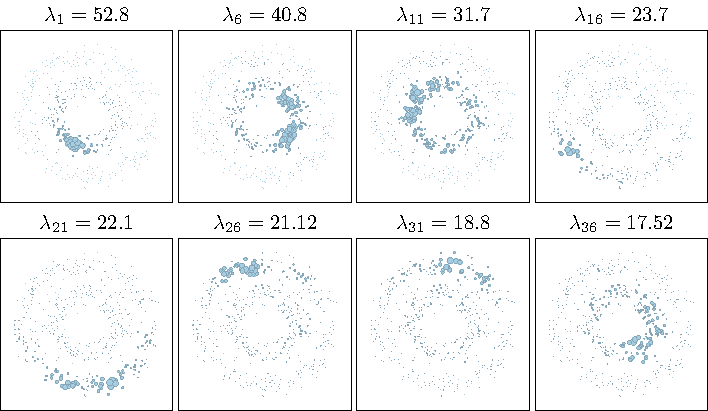
\includegraphics[width=\linewidth]{pics/SAProjEigen.pdf}
%\documentclass[preview=true]{standalone}
\usepackage{amsmath,amssymb,nicefrac,bbm}
\usepackage{pdfathesis}
\usepackage{etex}
\usepackage{xcolor}
\usepackage[a4paper,left=3.5cm,right=2.5cm,bottom=3.5cm,top=3cm]{geometry}
\usepackage[english]{babel}
\usepackage[round]{natbib}
\usepackage{graphicx,tikz}
\usetikzlibrary{matrix,decorations.pathreplacing, calc, positioning}
\usepackage{relsize} % mathlarger
%\usepackage{hyperref,url}
\usepackage{url}
\usepackage{silence}
\WarningFilter{latex}{Overwriting file}

\usepackage[colorinlistoftodos]{todonotes}
\reversemarginpar
\setlength{\marginparwidth}{3.1cm}
% Theorem-Umgebungen
%\usepackage[amsmath,thmmarks]{ntheorem}
\usepackage{amsthm}
\usepackage{thmtools, thm-restate}
\usepackage{algorithm,algpseudocode}
\algnewcommand{\IIf}[1]{\State\algorithmicif\ #1\ \algorithmicthen}
\algnewcommand{\EndIIf}{\unskip\ \algorithmicend\ \algorithmicif}

\usepackage{enumerate}
\usepackage{booktabs,multirow,adjustbox}
\usepackage[font=small,labelfont=bf]{caption}
\usepackage{subfigure}
\usepackage{pgfplots,filecontents,pgfplotstable}
\usepgfplotslibrary{groupplots}
\pgfplotsset{compat=1.14}
\pgfplotsset{
cohStyle/.style={ctrust,mark options ={ctrust},mark repeat={4}, ultra thick, error bars/.cd,y dir = both, y explicit},
densStyle/.style={cdens,dashed,mark options ={cdens},mark repeat={4}, ultra thick, error bars/.cd,y dir = both, y explicit},
primpStyle/.style={cPrimp,dashed,mark=triangle*,mark options ={cPrimp},mark repeat={3}, ultra thick, error bars/.cd,y dir = both, y explicit},
panStyle/.style={cPan,dashed,mark options ={cPan},mark repeat={3}, ultra thick, error bars/.cd,y dir = both, y explicit},
specStyle/.style={cSpec,mark options ={cSpec},mark repeat={4}, thick, error bars/.cd,y dir = both, y explicit},
specLStyle/.style={cSpecL,mark options ={cSpecL},mark repeat={4}, thick, error bars/.cd,y dir = both, y explicit},
RSCStyle/.style={cRSC,dashed,mark=triangle*,mark options ={cRSC},mark repeat={3}, thick, error bars/.cd,y dir = both, y explicit},
SCStyle/.style={cSC,dashed,mark options ={cSC},mark repeat={3}, thick, error bars/.cd,y dir = both, y explicit},
DBSCANStyle/.style={cDBSCAN,dashed,mark options ={cDBSCAN},mark repeat={3}, thick, error bars/.cd,y dir = both, y explicit},
clusterScatterStyle/.style={scatter/classes={1={cSpecL}, 2={cRSC}, 0={cDBSCAN}, -1={white}},
    scatter, only marks, mark size =0.3, scatter src=explicit symbolic},
nonnegScatterStyle/.style={scatter, only marks, fill=cSpec, scatter src=explicit,
     	visualization depends on ={\thisrow{z} \as \perpointmarksize},
     scatter/@pre marker code/.append style={/tikz/mark size=1.5*\perpointmarksize}},
pandaStyle/.style={cPanda,dashed,mark options ={cPanda},mark repeat={3}, ultra thick, error bars/.cd,y dir = both, y explicit},
punkStyle/.style={cPunk,mark options ={cPunk},mark repeat={3}, thick, error bars/.cd,y dir = both, y explicit},
dbssl1Style/.style={cDBSSL1,dashed,mark options ={cDBSSL1},mark=triangle,mark repeat={3}, thick, error bars/.cd,y dir = both, y explicit},
dbssl2Style/.style={cDBSSL2,dashed,mark options ={cDBSSL2},mark=diamond,mark repeat={3}, thick, error bars/.cd,y dir = both, y explicit},
mdlDbsslStyle/.style={cMDLDBSSL,dashed,mark=star,mark options ={cMDLDBSSL},mark repeat={3}, thick, error bars/.cd,y dir = both, y explicit},
% color change for embedding visualization (fuzzy clusters) 
colormap={test}{[2pt]
    rgb255=(166,206,227);
    rgb255=(166,206,227);
},
}

\Title{ A Mathematical Theory of Making Hard Decisions:
Model Selection and Robustness of Matrix Factorization with Binary
Constraints}

%List of Symbols
\usepackage{nomencl}
\makenomenclature


%\usepackage{color}
\definecolor{col1}{RGB}{166,206,227}
\definecolor{col2}{RGB}{31,120,180}
\definecolor{col3}{RGB}{178,223,138}
\definecolor{col4}{RGB}{51,160,44}
\definecolor{col5}{RGB}{251,154,153}
\definecolor{col6}{RGB}{227,26,28}

\definecolor{cdens}{named}{col1}
\definecolor{ctrust}{named}{col2}
\definecolor{cPrimp}{named}{col3}
\definecolor{cPan}{named}{col4}
\definecolor{cPanda}{named}{col5}
\definecolor{cNassau}{named}{col6}
\definecolor{cMdl4bmf}{named}{col1}


%
\definecolor{cSpec}{named}{col1}
\definecolor{cSpecL}{named}{col2}
\definecolor{cRSC}{named}{col3}
\definecolor{cSC}{named}{col4}
\definecolor{cDBSCAN}{named}{col5}

%
\definecolor{cPunk}{named}{col1}
\definecolor{cDBSSL1}{named}{col2}
\definecolor{cDBSSL2}{named}{col4}
\definecolor{cMDLDBSSL}{named}{col5}
% Theorem-Optionen %
%\theoremseparator{.}
%\newenvironment{proof}{\par\noindent{\textit{ Proof}\ }}{\hfill\qed\\[2mm]}
\theoremstyle{plain}
%\theoremheaderfont{\moon}
%\newcommand{\BlackBox}{\rule{1.5ex}{1.5ex}}  % end of proof
%
\newtheorem{theorem}{Theorem}[chapter]
\newtheorem{corollary}[theorem]{Corollary}
\newtheorem{observation}[theorem]{Observation}
\newtheorem{lemma}[theorem]{Lemma}
%\theorembodyfont{\upshape}
\theoremstyle{definition}
\newtheorem{definition}[theorem]{Definition}
\newtheorem{algSpec}{Algorithm Specification}
\newtheorem*{remark}{Remark}
\newtheorem*{example}{Example}
\newtheorem*{problem}{Problem}

%Operators/Commands
\DeclareMathOperator*{\argmin}{arg\,min}
\DeclareMathOperator*{\argmax}{arg\,max}
\DeclareMathOperator*{\freq}{freq}
\DeclareMathOperator*{\cov}{cov}
\DeclareMathOperator*{\anc}{anc}
\DeclareMathOperator*{\supp}{supp}
\DeclareMathOperator*{\minsup}{minsup}
\DeclareMathOperator*{\tr}{tr}
\DeclareMathOperator*{\bigO}{\mathcal{O}}
\DeclareMathOperator{\diag}{diag}
\DeclareMathOperator{\prox}{prox}
\DeclareMathOperator{\pre}{pre}
\DeclareMathOperator{\rec}{rec}
\newcommand{\Ya}{Y_{\mathcal{J}_a\cdot}}
\newcommand{\Va}{{V_a}}
\newcommand{\Da}{D_{\mathcal{J}_a\cdot}}
\newcommand{\KL}{Kurdyka-{\L}ojasiewicz }
\newcommand{\LXU}{\mathcal{L}}
\newcommand{\F}{\mathcal{F}}
\newcommand{\N}{\mathbb{N}}
\newcommand{\R}{\mathbb{R}}
\newcommand{\estU}{\widetilde{U}_{\widehat{CT}}}
\newcommand{\estu}{\tilde{u}_{\widehat{CT}}}
\newcommand{\estCT}{\widehat{CT}}
\newcommand{\node}{\mathfrak{n}}
\newcommand{\leaf}{\mathfrak{t}}
\newcommand{\krimp}{\textsc{Krimp} }
\newcommand{\shrimp}{\textsc{SHrimp} }
\newcommand{\slim}{\textsc{Slim} }

\makeatletter

\pgfplotstableset{
    zero color/.initial=white,
    zero color/.get=\zerocol,
    zero color/.store in=\zerocol,
    one color/.initial=red,
    one color/.get=\onecol,
    one color/.store in=\onecol,
    color cells/.style={
        every head row/.style={output empty row},
        string type,
        postproc cell content/.code={%
           \pgfkeysalso{@cell content=\rule{0cm}{2.4ex}\cellcolor{\zerocol}
           \pgfmathtruncatemacro\number{int(##1)}
           \ifnum\number>100\cellcolor{\onecol!50!black}
           \else \ifnum\number>0\cellcolor{\onecol!##1}\fi\fi}%
        },
        columns/x/.style={
            column name={},
            postproc cell content/.code={}
        }
    }
}
\makeatother

\makeatletter
\newcommand\footnoteref[1]{\protected@xdef\@thefnmark{\ref{#1}}\@footnotemark}
\makeatother

\makeatletter
%\renewcommand{\@chapapp}{}% Not necessary...
\newenvironment{chapquote}[2][2em]
  {\setlength{\@tempdima}{#1}%
   \def\chapquote@author{#2}%
   \parshape 1 \@tempdima \dimexpr\textwidth-2\@tempdima\relax%
   \itshape}
  {\par\normalfont\hfill--\ \chapquote@author\hspace*{\@tempdima}\par\bigskip}
\makeatother

%Thicker bar
\makeatletter
\newcommand{\thickbar}{\mathpalette\@thickbar}
\newcommand{\@thickbar}[2]{{#1\mkern1.5mu\vbox{
  \sbox\z@{$#1\mkern-1.5mu#2\mkern-1.5mu$}%
  \sbox\tw@{$#1\overline{#2}$}%
  \dimen@=\dimexpr\ht\tw@-\ht\z@-.8\p@\relax
  \hrule\@height.8\p@ % adjust for the desired rule thickness
  \vskip\dimen@
  \box\z@}\mkern1.5mu}
}
\makeatother

%----------box---------------
\usepackage[many]{tcolorbox}
\tcbset{
  myhlight/.style={
    colback=cyan!10,
    arc=0pt,
    outer arc=0pt,
    boxrule=0pt,
    top=2pt,
    bottom=2pt,
    left=2pt,
    right=2pt,
  },
  highlight math style={myhlight},
  mybx/.style={
    colback=white,
    arc=0pt,
    outer arc=0pt,
    boxrule=1pt,
    top=2pt,
    bottom=2pt,
    left=2pt,
    right=2pt,
  }
}

\newtcolorbox{mybox}{
	boxsep=1pt,
  	breakable,
  	mybx
}


% Zeilenabstand einstellen %
\renewcommand{\baselinestretch}{1}
% Floating-Umgebungen anpassen %
\renewcommand{\topfraction}{1.0}
\renewcommand{\bottomfraction}{1.0}
\renewcommand{\floatpagefraction}{1.0}
\renewcommand{\dblfloatpagefraction}{1.0}

% Leere Seite ohne Seitennummer, naechste Seite rechts
\newcommand{\blankpage}{
 \clearpage{\pagestyle{empty}\cleardoublepage}
}

% Keine einzelnen Zeilen beim Anfang eines Abschnitts (Schusterjungen)
\clubpenalty = 10000
% Keine einzelnen Zeilen am Ende eines Abschnitts (Hurenkinder)
\widowpenalty = 10000 \displaywidowpenalty = 10000
% EOF
%
\begin{document}
%
\begin{filecontents}{circlesV1.dat}
x y z
-1.0583288758102631	-0.20196401315764936	687976759029136e-21
-1.0549650952895588	-0.1453486277315127	7386196123201584e-22
-0.28686705420107594	-0.20577169621106567	0.17815435844407024
-0.22438385123724203	-0.6311838265132071	0.21592100451587828
-0.016329900725535695	0.8363156387087571	2674319214850201e-21
0.6664943110916062	-0.02522611869462293	0.0005527513587903361
-0.7000695186307817	0.8524609054729188	29529351835749036e-23
0.8737756445548316	-0.34343872237549916	3709281555963715e-22
0.26863712824940233	0.621230160725688	9076753978737366e-20
0.4135070890114797	-0.23094514442380681	0.00601075192492206
-0.8374130044011527	0.6731231597212262	17538278472700352e-23
0.6029899953791354	0.5490490339208243	9952071219487522e-22
-0.07532043439212403	0.4864515282258869	0.002931357139329265
0.38404755622047315	0.42223071846853666	9698024916316254e-20
0.5552969916156367	-0.1083120535732651	0.0018297134498240007
-0.21526850262358294	-0.49881387813462996	0.8946943548726807
0.0005701763274310358	-0.8608567301737946	0.00010661858325044138
0.5659515908300676	-0.16181812669682585	0.001850114873467643
0.7402734062213887	-0.7200478091020212	4925783986675728e-22
1.1196812938139424	0.34846871970260435	1596396947341649e-24
0.9436364508675184	-0.27253854831430324	5314624951671693e-22
-0.24546029448781795	-0.4906102105866899	0.78763669818148
-0.5666890574615214	0.8469922677428234	6202036475449384e-22
-0.8121420956043262	0.04089898834206568	0.00015379010534739392
0.6925296824873941	0.5004844069787805	973304360974059e-22
-0.7802845097289287	0.6503350319668115	5576970993205807e-22
0.19540149773912174	0.9988933466475728	24443428756964744e-24
-0.49033960699830575	-0.745615965610353	29325642970168703e-21
-0.772379045803115	-0.5555503478357138	24660986207932743e-21
0.08949600849053171	0.43569426601040284	0.0006895437731731368
-0.2709014254935288	0.8329314883710439	1858667573484484e-21
-0.4724968520274526	0.39757762314794287	0.01400469907519787
-0.05076606623229138	0.9472731081345089	4849786056715719e-22
-0.4244181110366452	0.15163647468601898	0.05710547728093898
-0.856823736320482	0.42050645578658474	1940309304990451e-21
0.3801522274867655	-0.5242396510380898	0.01085602302957319
0.5302560693756595	-0.046308947018418645	0.002341799906206716
-0.0592471029661714	-0.8742925870679111	0.00010851122957934113
0.9136426992044209	-0.6268351541350334	3780614075344911e-23
-0.8755978758264108	0.47329951242226026	5595983976092128e-22
-0.4611459366222198	-0.29641002189383403	0.26089658989048303
-0.037954030937970715	-0.5674223028442248	0.515173242934422
-0.2144341080960731	-0.940890046876266	25292234206844616e-22
-0.15386158302832836	0.8539796415576204	4019652964257018e-21
-0.34600659981207815	0.22605644970598238	0.04294469927408564
-0.5581576930234105	-0.014719460229306036	0.0365112394640575
-0.8197754374675081	0.717359733882507	24995078415116687e-23
0.27775250685348385	0.18189032091007415	0.0003456898491932029
-0.4029746673951193	0.1027363359902787	0.054062044575186104
0.4968916538935379	-0.000844611354336014	0.0020705980157979553
-1.0774087697285004	-0.07678224474566575	6851299550051645e-22
0.8614353478008437	0.025271734377208227	13743177148474474e-22
-0.801406799115663	0.5601142307444397	486585993725284e-21
-0.4793204129385923	0.3306162943293071	0.031592207237906685
-0.6015487302066529	0.1320612905764609	0.023855541942386475
0.5617427965558156	-1.0113021326424354	3102206428439462e-22
0.730444208221491	-0.6768972250254602	79721244503304e-20
0.5214794214363629	-0.5008727775322623	0.000616275463520605
-0.07937288077704525	-1.0020594043483257	29665956424782087e-22
-0.4105200259369002	-0.863231624107107	5087349582846109e-21
0.3388762765570134	0.08706717470919467	0.000800695098908496
-0.8685030533130447	0.3738037066733266	2135906788251181e-21
-0.45683545912363355	-0.04267855156658711	0.05025966850123004
0.7512915187942618	-0.643291765899665	7172604804742435e-22
0.6216335172514909	-0.11511316015280951	0.0009571941646840217
0.2989142354739267	0.39780163534212587	0.0001476829361261019
0.8832260533811114	0.5378029603982082	1479687188643962e-23
0.7706147096701259	-0.5688688999070458	4262228438259068e-22
0.7777354887198962	0.720528533564723	4310908190388121e-24
0.33650550115674555	-1.115393724949389	2290487646665865e-22
-0.342570290724111	-0.21142060265518764	0.22021156641099834
-0.25812602086366604	-0.36207505076781854	0.8291244748424244
-0.440512439401967	0.41982647549444946	0.01356126625467441
-0.41029305865551974	0.5613483829060184	0.0023760934755905102
-0.5385119865491543	0.854068737227722	46804921608284784e-23
0.28817771225733035	-0.35555608208892875	0.02114774704461659
-0.46394391030820226	0.9413388577320934	3035129735682728e-22
-0.24831840720533802	0.5237809077418585	0.00435086555720168
-0.6552850605832186	-0.4599331054248453	0.00026446562713125705
-0.2826163494076298	-0.9757361666246253	6395291442346341e-22
-0.3774044986295204	-0.15754990126458723	0.1718272412396457
0.39289772381826926	0.21639482757710704	0.000545843947319971
-0.3000684974285963	-0.9288792097716005	999220901377361e-21
0.23230106715972593	0.5053020150438099	0.00022389340314926402
0.035704278426334946	0.533270659937437	0.0011356479147815724
0.09598775875172952	0.8618425666792344	3289196704723673e-22
-0.17962630292512827	0.5212494227356729	0.004244832384434762
0.31236804409574365	-0.34388834400933016	0.02173315701702628
-0.47976322944270716	-0.5787808073254304	0.019263259308459565
0.6093508783156708	-0.6552395783902365	46348541971280825e-22
0.8464430922888276	-0.6582476883085377	14449881885219646e-23
0.30952844675119945	-0.30050993673209625	0.012161864593158473
-0.35579373024330907	-0.3031730669351904	0.4458458843024813
-0.4729710467200588	-0.9161905551389896	36764422000724584e-22
0.8105489062223111	0.3063890203748192	4228985253439654e-22
0.26349519971405094	0.3154986373224412	0.00018491240430886226
0.151915912568039	0.5325519003756559	0.0004903229320341736
-0.10319754741500724	0.5493951282610205	0.002520222749767573
0.9203553330570633	-0.29254729468906093	544644299707871e-21
0.4831799702244233	0.060377797979320996	0.0016944222991926773
-0.5796183887393597	0.7746200654923161	11511741541783402e-22
-0.8541885431589489	0.5178310337137458	5635530289048223e-22
-0.8796583444738513	0.7081111554312315	6249669180532147e-23
0.34083406290250495	0.74696794539091	35780357527016524e-22
0.6438062065547421	0.684737062537711	4602542477738397e-23
0.8167936695881719	-0.7568243617688544	1396508794667108e-22
0.4246697255417251	-0.3328124636208833	0.008137675043241316
-0.9859854354757545	0.26344939470473255	8783425379292635e-22
0.36302398095734684	0.2746590061351894	0.0003293231807867095
-0.025297734684784023	-1.143907353283561	19392146342097465e-23
0.2032554345955354	0.28830564392732866	0.0001767967276239974
-0.2502433512821886	-0.41755435063352553	0.8595418664544406
0.5098578452924067	0.4695047239790404	22089329689357823e-21
0.3443787337008237	-0.4675382901965091	0.023181377978022166
0.9881522604297938	-0.3021471510603488	17056016447195702e-23
-0.48057110152907556	0.057853088635956826	0.05312845903214104
-0.1494073465765274	-0.4744536378002139	0.9763040372169911
0.2291058540766086	0.6877816124566098	3105363401895568e-20
0.10432827601608814	1.007003579269503	6085989839492026e-23
0.031436823141421995	-0.3070447159882047	0.04152011647189512
-1.0941411050076675	0.3821308374739647	10485243622358463e-23
-0.006772415554554288	-0.3403823630501911	0.16983310846608035
0.03790459976473807	0.8981000637907597	35311524580968386e-23
0.4724071282898181	0.3379026545362105	0.00011841588859968858
-0.5687164572253783	0.11499339914612097	0.03221656236486325
-0.08693938008162763	0.42279389507717124	0.0032787064363513376
-0.28689351236975014	-0.37462850605791104	0.7534021056043091
0.8626364254896491	0.3878238798233949	8184937491350128e-23
0.2454241460431366	0.29822889729914215	0.00018359719026852524
-1.1331872257168936	-0.014302927588677045	4201528432229772e-22
0.4474309277283363	0.15150716280611207	0.0010735944019490083
-0.9952111212193668	-0.2692696791591609	385953350634431e-20
0.33451824342581943	0.22445047758195008	0.00039345008517963174
-0.45141735558253765	-0.5264915335380573	0.06342766350799213
0.14051117817071368	-0.9453552208299545	13285816599531553e-22
-0.5491877812265945	-0.801112192863598	29481655633360168e-21
-0.9863368691505784	0.41417098820521786	440638274728957e-21
0.27278308023328324	0.8296836984169661	11197993566709313e-22
0.1891406899596204	-0.27355388028025107	0.012542774385133898
0.5534652549685908	-0.5958867421206311	58519086256949506e-21
0.6847207172590709	0.5463728715139321	6590444860887072e-23
-0.37443413523697894	0.8760256040266927	43363477961552595e-23
0.4392548163834803	-0.9047561020319701	4053222477195189e-21
-0.19545855718707983	0.3152184994865719	0.005379575921434386
-0.9941933253410392	-0.3165529558686342	2884762905638684e-21
0.90768322436734	-0.39962363443787496	10116057802616773e-23
0.21606973625964263	0.537937900067448	0.00023694358612409401
0.17926414498256826	-1.0625373062111834	3698747480520882e-22
-0.3842822926705394	0.07890580561977101	0.04717942274259274
0.9483542004901386	-0.35261244440864314	1238497825929383e-22
0.4937510937461273	-0.7512057092701449	15807309382772896e-21
0.002194023717617566	-0.9067718398812545	927952450666516e-20
0.04853172316213811	0.47150668085564584	0.0010778721229098935
0.058687648748172734	0.5599084359157949	0.0008889804752103101
-0.5342332606475368	-0.07309364796671353	0.04791367456264743
0.9166764532207246	-0.17096965575209683	962543774948631e-21
0.5560622463214425	-0.19500798744869144	0.0020726469919232294
-0.4508337971767867	-0.27343096232028685	0.2866015935145675
-0.2249770521470013	-0.977120879775083	6113584380321109e-22
0.5105063250464269	0.17053921152739293	0.0008519259455008477
0.22610688378803662	-0.9577438670294672	9667542071847555e-22
0.7003486506302466	-0.15180173128212845	0.00017500360464815088
0.006636214456188352	-1.054807062255213	9673044514861463e-22
0.2584532151158738	0.9829378520319795	3397965978994049e-23
-0.4557941617257688	-0.24674411027449922	0.2333426179815954
0.7116187117871964	0.37399667612376497	42914279469372275e-23
0.44253310209306695	0.9491491060163105	22845097353449053e-24
0.08447685192909979	-0.8351535915539824	8863881369857815e-21
0.5633797515703941	0.7560384738182708	2287815571356609e-23
-0.9683305242013036	-0.5729099853696185	31171470747517634e-22
-0.5127125337250293	0.8022392827607193	5712020073187479e-22
-0.4025752704584875	-0.19586338037814632	0.2062791591580176
-0.373579961679699	0.07076226765469532	0.04549910227224119
0.5847086359226571	-0.10428584342601002	0.0016052238979785368
-1.070192755078586	-0.5175893695396888	25086075757722183e-23
-0.37585788050259117	0.26622981099006604	0.047481323865519655
-0.04153066411364073	1.1298070647975962	7820480026369863e-24
-0.29849855076934684	-0.439235662946394	0.7611457024134005
0.7986762407696741	-0.12350308057782419	21420021396020292e-21
0.7241725359210982	0.7673470713309014	4154611593008038e-24
0.4425716175145471	1.0545877925203901	4517520327075642e-24
-0.3009942479406195	-0.28544465808629016	0.4287049418161772
0.28456936812944295	-0.3657137258550358	0.02178806099028045
0.28744578929175285	0.32854425576712576	0.00020631417959207136
0.639937762556447	-0.6505099028952075	45842621664898e-19
0.05823208873356708	0.9054436486403517	3546041876317958e-22
-0.18827083294877459	-0.5175564452077821	0.9108231492033209
-0.9329068382156008	-0.3801321106596237	7599034298521216e-21
0.5601450967893756	0.09698845485225183	0.0011501551043251112
-0.3756527474612627	0.7120960532866892	33185441842445497e-22
0.28648170510331256	0.3442269536180647	0.0001816900204669042
-0.5545045803725894	-0.854004082386823	21986593367885936e-21
0.27939838551695295	0.20316442364718562	0.0003159342689058843
0.16904383170478116	1.1363146779633637	3818200530662629e-24
0.41960093047149866	0.13705185266873904	0.0011431353965622292
-0.4498033980116379	0.22672303751202222	0.05392730270001006
-0.5081276724502488	0.11652282996013652	0.0507943901058836
-0.04972504364164415	0.31835178586661395	0.0009590992975685355
0.5272444182086248	-0.7879070986907416	35335175549696355e-22
-1.0654861621254115	-0.23509318286565328	6635511712047088e-22
-0.9887302337932489	0.1103754459557201	26500360503268926e-22
-0.37771282161869674	0.2089104993471779	0.050017634593180246
-0.592996935730106	-0.11660158192407682	0.023890116357875843
0.7777222354165501	0.5099416601581699	4396283823693886e-23
-0.6597553949317734	-0.01980472153961566	0.008471011535055478
-0.20893659613357207	-0.48724539646942766	0.9093488753578578
-0.8068455521466513	-0.29997047342039707	0.00018838146789521966
-0.6900745319305372	-0.6280428506278541	16848631006253368e-21
0.8614051450394694	0.267928431998897	40055656222127127e-23
0.5913328927145274	0.7855026465857798	18151196036025133e-24
-0.9217563671575004	0.24534492193834448	51211060882629775e-22
0.38474371433279925	1.0935616549059102	11715554962536724e-25
-0.46741030056521377	0.2591755254370145	0.047260072251211815
-0.0381025675995942	-1.1251543679349862	37290299289886735e-23
-0.6243967254451009	0.46517409634094015	0.0004450085339160657
0.21707179540902807	-1.0140863576742312	5613798829727398e-22
0.7081813705522666	0.7162885127966534	9815410449997586e-24
-0.9451644776861263	0.18394464444693226	675828659555267e-20
0.3729334539383104	0.46088009666634666	6615299130200575e-20
1.0696979889031235	-0.0794841459498074	3932366594472406e-23
0.7555529047587174	-0.6789645529590862	7509897735164391e-22
-0.4390917083090098	-0.2160668681154164	0.1919587106072599
-0.9161126914457096	0.5398116209231641	2355536972473724e-22
-0.7407788219528375	0.33551254951641335	6814936689742698e-20
-0.2114261856758002	0.8187152036533841	9754638719501758e-21
0.701545668282712	0.08200865693028041	0.00014349153405292093
0.033338468862882234	0.6199041811295294	0.0006183926814249463
1.0748984302382512	0.35907777637212224	24252781344128707e-25
-0.4597850556976463	0.045223030444219284	0.05378463338264669
-0.1741463993378947	0.7865778186239607	2076249229881262e-20
-0.33728863860345176	-0.35849990456630876	0.5715513853651248
-0.9587665698372234	-0.42543103080047867	4982111203084549e-21
0.2123157690598867	-0.9860875988345833	9943151121386175e-22
0.04602382173605105	0.9088619887209635	35689148418546146e-23
0.3725537615240344	0.1876685667278354	0.0005323993176489865
-0.8740700379235082	0.31983625072337724	394396413912705e-20
-0.3892066741361861	-0.9811247119391876	9022825157028842e-22
-0.8474412504983133	0.4654098218172844	621389379436518e-21
-0.5108698639619283	-0.10057435621987655	0.07469706863746083
-1.129071205600398	-0.17027012619747586	31562111412901e-20
-0.39514507247834857	-0.8103936481837801	18745432055901755e-21
0.4704996641617121	-0.17220690970158825	0.003556735352217171
-0.37983945734932445	0.12041154024224539	0.051664067678708306
-0.055472740425509856	0.6206042795137554	0.0008418593987128163
0.3645979153047041	-0.41706786292712994	0.016175952871092067
-0.015561824056395212	0.8198043684673366	9080030140413172e-21
-0.44145592026764	-0.2505282912308723	0.25369889110765625
-0.2561401471320713	-0.40112951606947655	0.868624467749652
-0.52338679166547	0.02660578819265639	0.04203722911495992
0.21445818450520165	0.22082326083082776	0.00012745893534484232
1.077569058206745	-0.3491332068383815	24294410367272213e-24
-0.1872746787626816	0.7899535223817675	20784101599586684e-21
0.290127993873019	0.8394507724623782	5433619158280008e-22
-0.8865250322253393	-0.08940312375709093	12815819843474678e-21
0.8621507749457712	-0.34819857547136623	33691481252205987e-23
0.18225473918119706	-0.28728382873787084	0.016627101983279553
0.4654196763131379	0.8563057194157547	35354340194794333e-24
0.8303630898153743	0.36063100311212853	4261839446174578e-22
-0.9712638110423526	0.6382288332737301	4610470515973026e-23
0.23666688614920567	-0.45266804798952437	0.04883570289213089
0.6309050357598261	0.7240590312014205	2189050024184943e-23
-0.42767689370476714	0.9491438031378565	27959047081350044e-23
0.44563927184415986	-0.2274601203045902	0.004055105894582521
-0.2053874739053867	0.4253844412184107	0.006999073334742131
0.5405420315871583	-0.15236975471038613	0.002264857191687393
-0.26241022071698467	-0.4527201725965245	0.8259953110261454
0.3800831916990306	0.7125239676567952	2747050491258512e-21
-0.5746742466560214	-0.14252620560541895	0.05383982994058495
-0.353711250098192	-0.089227175639014	0.07191632903369924
0.9454568469815224	-0.6882256956905914	18858202044905343e-24
0.8557340217873753	-0.6560332493577736	12413542577632616e-23
-0.556562516437247	0.025216778123066684	0.029636692173030495
0.636271359519193	-0.1412312507678136	0.0008490835190640259
0.45228206748941496	-0.1464962121039572	0.0038779608259858407
0.29958240361829125	0.21950393236552065	0.00032678724139989447
-0.48441555279257537	0.9138234923246589	36988856457648106e-23
-0.4461707440833614	0.9247836035865585	33862623315730784e-23
-0.4201939672191152	0.147701646190593	0.056219461075248264
-0.6425112593179262	0.8853425199869299	29945495045399257e-23
-0.9942338743953323	0.29442352385918036	8801715505268484e-22
0.5984091164639631	0.6507722124429921	714916688724187e-22
-0.44739056708622243	-0.19530513215445594	0.18594593894638917
0.10544312980633214	-0.8886995454263548	7148358125200326e-21
-0.16519124887174855	-0.45974106532199166	1
-0.1452578553741265	0.16491959057663946	3047328413428026e-20
-0.3271832988321618	0.15469783349016974	0.03858780214821989
-0.11311105980459281	0.9135157952010174	18548674626427548e-22
-0.3561083380389497	-0.2947817783686462	0.43490223268456263
0.3724658234027415	-0.9915409863714767	19093619049110764e-22
-0.809763642248029	-0.12327687501896292	0.000205460495855068
-1.1287681161906478	0.06262847595617371	4447570461916485e-22
-0.6997744034861316	-0.5562715236294364	321238374472271e-19
-0.686767025909816	0.22799527222288463	0.0032908344832878376
0.718150173365836	0.614101346547797	4810628078802753e-23
-0.45660502262193225	0.30925490188894406	0.03654263012800704
0.5685590020433319	-0.7691628640835012	37089941523937966e-22
-0.21120482990041983	0.8920372566221498	19091548390033314e-22
-0.8559997833581601	-0.10979459128678692	28031286631626762e-21
0.020241236020441977	-0.9871905648513019	5233264691499702e-21
-0.19378550438170256	0.529549096346015	0.004189846077931001
-0.48576133985104347	-0.7248762853196216	0.0003870570902795034
0.39513367611481626	-0.8885158369058909	4013030238357137e-21
-0.18721242838064622	0.9702879441616987	4061731354601975e-22
0.8396921444402687	0.3365818412168194	4257295193632143e-22
0.877467440180306	0.39080964030788956	8163289024795694e-23
-0.5499282479717139	0.5999930092507813	0.0002453651908515492
0.39606976564711266	0.01353375952124733	0.001921175892101656
0.9408685147764327	-0.16839212966354405	927685777895485e-21
0.058529813294819356	0.5960832480212296	0.0006970806883852174
-0.3085264124619913	0.867923991978884	11630369001701663e-22
1.0240606495199067	-0.05902106596557902	5743996584054494e-23
-1.1297448788625983	-0.08852295833376425	31474134293741186e-23
-0.3019985141368995	0.30893831800591814	0.02148092657522364
-0.008533740271034915	0.8593779967999691	26743192148506146e-22
-0.47766065242119404	0.09174102825933139	0.053326782742638565
0.552796931763394	-0.07589565750634704	0.001794377375019225
0.603572742486676	-0.6831181382142064	27953295513778685e-22
-0.33288992349487256	0.13169527999030434	0.0381908937319041
-0.2390174716089229	0.7900359421455263	9678838125683676e-21
0.5308565325208349	0.507359333449821	14512120551653933e-22
-0.24541435549726867	0.2808122025738658	0.012972853067883563
-0.29898976544354733	-0.7827067523032034	23205358915273614e-22
-0.9999570201344817	-0.2026055094073493	19218286705388836e-22
0.29758558346109265	-0.36715492999328203	0.022011315054850197
0.8674564090945402	-0.5819678100623382	7300557334568551e-23
0.600229072467383	0.22647599269832278	0.0002640674878813101
0.20769676592782566	-0.2429673540455613	0.009091238993045177
-0.16980961206235062	0.44328283958495246	0.0056152346685033865
1.0742084655937019	-0.026185528019472687	2395117173137954e-23
-0.5990364456171003	-0.025393658161253316	0.023284081960375434
0.38651874675910325	-0.0313701916023475	0.0020250973270705226
0.5347630915993977	0.17166579010558058	0.0006803294001614598
0.3815611790828055	-0.15397406983635387	0.003539563791397765
0.5058927256985234	0.23791877175557427	0.000445429448111775
0.7572842422665051	-0.7254577812166593	2711129700603262e-22
-0.9360697829922907	-0.35462224573950774	8446580525728072e-21
-0.14478358844783776	-0.9498460059976374	4599607947932434e-21
-1.0228407301441125	-0.0018387135408612018	18337106716486614e-22
-0.8185514119556835	-0.5782789864229126	25249665647817257e-21
-0.5190222237533468	-0.14121284297452863	0.1028600154750412
-0.8812420477325542	0.09550201023389113	40016075000964435e-21
0.8043770929313652	-0.3853011709405064	7844353685356873e-23
-0.03568713716803138	0.5775112808391898	0.001052068480834077
0.35582627317999016	-0.23527882041840337	0.007848792361647905
0.07420419694257939	-0.9294188883144827	936455577470905e-20
0.1662899576554404	-0.5284808316844934	0.11435967878366314
-0.3572795738981698	0.8443053913527945	8495652087924456e-22
-0.9577523664409258	-0.29415179908865413	38797365753035585e-22
0.4986549895301416	0.7233237313187797	18215251804223754e-23
0.11984529006189726	0.4304757087557079	0.0006430562344810005
0.677209428557069	-0.1968148144685232	0.00025867260699753323
0.353158843408339	-0.2294141726153695	0.007333860472072097
0.6926163091663033	0.9082438486259222	13305959399929301e-25
0.22662062842571284	0.7101939697778475	20075135248296205e-21
-0.6173942947547322	0.6857369967943334	12522140833141256e-21
0.9361950579940088	-0.5613127488775519	23371465170677977e-24
-0.127424404632568	-0.4268659769339036	0.9470742298344268
0.26174039678270733	-0.21335055076531645	0.005052909852641206
-0.14895845969227897	0.6038885892071426	0.001210755093556201
0.017206819968116654	-0.5610869042333229	0.4492943805497979
-0.6165701158875304	0.8039827900466703	11415465984723164e-22
0.3368370747340216	-0.6011912237933033	0.007152403389712189
-0.004612791244162896	0.47514382808152794	0.0014565744474741944
0.01843812087421645	0.4484493986239611	0.0012451060806369604
1.0102123569818526	0.5165463334857523	3459898079000362e-24
0.7972873049177899	-0.3639915217251992	3108190296152853e-22
-1.0664272738526281	-0.0883863999456583	9867603922124017e-22
0.6426248444603162	0.14819452862153007	0.00029402028233657196
0.9008961948591205	-0.638870305850429	6164685718501925e-23
0.07864578043864236	0.4429924687743171	0.0007596960583895402
0.24736111985778403	-0.46837324136874914	0.047338771279151946
0.11571675991762002	-0.5488435993368718	0.1405660195860155
-0.25999785574842316	-0.4648227479797838	0.8171098552433961
-0.1282785387957175	0.8005039835738349	15054905229340922e-21
-0.6941747414267789	-0.10895464287467746	0.004312198405479585
0.5643296830461592	0.41564751900823327	2560482462376823e-20
0.393601640931545	0.8965530173420195	8683902061530899e-23
-0.6242684592992149	-0.68783187626963	2848182522711646e-20
0.4054686352399301	-0.33391817631930143	0.009547506139647546
-0.3861661312630557	-0.19434905522093565	0.2119605677175169
0.9141444978148033	-0.2052575568430186	9391185936522531e-22
0.2569409389934234	0.22066279246844922	0.00020733269874683412
-0.3406827094916554	0.3943071650929997	0.0183394286358125
0.44542838045587774	-0.9405066295787441	30110864746728865e-22
0.486743607490183	0.010295075115063876	0.0021404602577832807
0.02567392299065019	-0.5353718854477386	0.4483566618438325
-0.15396452356596207	-0.8301000411980569	0.00010398553884257198
-0.46406039285362755	-0.07011817763253647	0.07002335647420559
-0.1654591278460084	1.0093935572815773	2454795074912324e-22
-0.741574685169897	0.6075049586400391	1370569164644704e-21
-0.8839504856898732	0.4843707069263513	5493270439024073e-22
-0.2772708916507828	0.4271776286910839	0.01123446670264895
-0.007915654790254648	-1.0374245659643888	9900160936166507e-22
0.07158038113892838	-0.4470777829690491	0.2715891058495441
-1.0979023568400463	-0.2788707017013692	5614168785743902e-22
-0.8383403144319864	0.47642383134293137	5280280757576092e-22
0.6722758352720496	0.7407194847455977	1170497785388399e-23
-0.04462100192073412	1.0253515873635495	1231048760883581e-22
0.3059243103815058	0.30551382614764	0.00024254233462774998
-0.5007235364262262	0.305162592217073	0.03042068599887004
-0.04835433089425645	-1.032045099586184	8503059139984857e-22
0.5223335457063931	-0.8001425195591133	3549049014251947e-21
0.24149010192315168	-0.8715983385787441	27572129603612808e-22
-0.7942862878598648	0.7355786621547904	510020427863332e-21
-0.5840637350131117	0.35352633664496064	0.005379523945150776
0.7666697426076825	0.38792851703849934	4402781839135756e-22
0.3602768399720905	0.11065682747370947	0.0008846523870060412
-0.33762463156101746	-0.29981653068887726	0.46631415809517973
0.7413270931177445	-0.8012725814158732	16851719139909864e-23
0.41530854244488424	0.25140265746432494	0.00040768117063939846
0.34830580483963713	0.43593266031629013	9173828658035996e-20
0.4481077666063202	0.5022198174529555	219337324674145e-19
-0.07078374784853891	-0.46365027125240593	0.8370576560819322
0.40691344638633065	0.20194743468366066	0.0006157753406298368
0.26473797616138184	-0.37970123656838783	0.02726137508491243
-0.3430075566496395	-1.001014309078478	5630847162846604e-22
-0.07098190777517646	0.49124527294967674	0.0027048990383244167
-0.3696423277599601	0.9311821284465949	35858795735623594e-23
0.15781888335557667	-0.818076320322263	27798766320672534e-22
-0.012063147114350647	0.5015628247807506	0.001518508787955284
-0.5401592010556218	0.886425655241674	44736322079676597e-23
1.0143693052313847	-0.13847113343398026	12767918771486876e-23
0.5426832353988738	-0.028865776093147645	0.0019397705015600844
0.019493189988530002	-0.35211917974380724	0.1579499087200321
0.39796033385805474	-0.21653420832469542	0.005674400855326473
0.06932313386297567	-0.4650929980884387	0.33826381069191547
0.3855920910769304	-0.3703680740548607	0.01181400512001456
0.07668961878948749	0.504487350499383	0.0008379949952606556
-0.41590152051588525	-0.38590385766809937	0.3685038305946393
0.5112713182857704	0.300526008214048	0.00019970580190103307
0.44278962454753035	-0.12582498230716915	0.0037053577283125924
0.3587073438595803	-0.924707220336543	3895358939117396e-21
0.9819876679370327	-0.2645150004065293	17842828656976446e-23
0.042515674170929135	-0.7902031675276707	0.000106406537264838
0.9842189549691335	0.41115896420360276	15050140966378974e-24
-0.4339910269991673	0.15042822254012278	0.05849108155534333
-1.0664501738684824	0.05611953902551445	873346533665334e-21
0.12381363799397313	-0.2906794546712879	0.027010669548066864
-0.9287624426681778	0.2980361842691943	26256279163715315e-22
-0.32467663804828306	-0.37282219809450984	0.6203777003331049
-0.017267746630876546	0.30114051365578065	0.000543642719938363
-0.20322929100860568	0.34196259635971044	0.007093012344065527
0.6149295803569534	-0.6574878070065425	4569000422389517e-21
-0.5019331683517144	0.5034120088464493	0.002667478067261255
0.37959496422941374	-0.19817478772397484	0.004955023245102079
-0.6288413136352182	-0.0686225510329849	0.019160498081953005
0.5576922952499451	-0.7372777659850459	3834510157275666e-21
-0.7473156621355121	-0.35958003748297923	0.0002031576215397001
1.044766441941261	-0.1640132387701801	11056882933297713e-23
-0.5248584449224766	-0.1626584031102783	0.12558797543043734
0.5468339285697519	-0.8515486695216632	22604546595215726e-22
-0.8488608547924452	-0.5277291713396844	1896942884631836e-20
0.09129344106845708	-0.9929084269568997	10749879579513075e-22
-0.8133312932653112	-0.4325977063875221	34821546650800266e-21
0.42790218086737897	0.03368246917509174	0.0018544695110320197
-0.345703241038376	0.2669186991384062	0.03976606218036156
0.3743264449179663	-0.5437708269458819	0.01033215796419803
-0.771818816673675	-0.23721045607514987	0.00084048432996943
-0.9459166240312367	-0.5947562706827852	3610010714120574e-21
-0.4543408316958324	0.4716252527218408	0.00715106629933941
1.0190866335789526	0.3711877245816759	917414733506956e-23
-0.21781367160080423	-0.4364787637053435	0.9199098336426929
0.6694831669040802	0.16780314195860563	0.00022372796532751807
-0.11334332903498678	-0.30867673172262705	0.2643272881128332
-0.8479602054835725	0.5928559189151142	1952476625479501e-22
-1.0044694724664094	0.36164690812566047	5642233737966592e-22
-0.6964101427144668	-0.04329881702200409	0.004098582604578063
0.15553838290615063	-0.4545474031281862	0.12305900514671539
-0.6330956374343583	-0.8230604228089214	13339054795646677e-21
-0.834071330279343	0.5284489610165986	5404697472980327e-22
-0.7603398421567891	-0.3478439515517804	0.00019301927089352685
-0.14599715053105988	-0.41447742938148424	0.9368054283078172
0.7985840911794406	-0.8416644620776599	34257821649128504e-24
1.045546872577677	-0.32961473056675883	49426900900327206e-24
0.9216600778725588	0.19676141715944806	16546583973312568e-24
0.13536177018969225	-0.5654614405280538	0.1255426913994526
-0.1467968113274581	0.9327024933348684	15836906155103976e-22
0.8828512011106353	0.3995720345410485	8163289024786591e-23
-0.5250562446249011	0.9959137054261278	1354190720399071e-22
0.4444706003292941	-0.08613466876944118	0.0031763205215376124
-0.03651906329943556	-0.5776097455166717	0.4678789998948669
-0.18275922882623855	-0.36911929361528273	0.8181541060429669
-0.008357904929132312	-1.0400712136700585	9900160936166515e-22
-0.46490602896191124	-0.7521850939029222	2886200117989813e-20
-0.8629666931629013	0.5586407994356856	40959839211027205e-23
-0.6494376078685997	0.7979569864308408	10651357094365384e-22
0.8100743508008097	0.5222176894097934	4523046579280407e-23
-0.4763513992824499	0.29435036447461255	0.03905780080102962
0.9968051748529907	-0.2575222892887514	1644969149756686e-22
0.5242050451376069	0.8022664649393088	2682182210941204e-23
1.0537007610962097	0.04186827819127899	12989114043954501e-24
0.6866816563190805	-0.6998664005357831	12834126448337089e-22
-0.8686423707348288	-0.2343643483529707	54073642805727994e-21
-0.40482879492639007	0.3791464480343506	0.022123287344186702
-0.6514563822495386	-0.8843925992284258	4954530228030426e-21
-0.6751986838155158	0.6808714231615992	61764334561856435e-22
-0.17206390120164555	0.484188774179118	0.005101567851704851
-0.1777624864565969	-0.9108790982123965	4609330419878977e-21
0.4561691628917222	-0.29274091655163537	0.0050242086390658155
-0.31002924981632496	1.0304684380914757	13404659576895345e-23
\end{filecontents}
\begin{filecontents}{circlesV6.dat}
x y z
-1.0583288758102631	-0.20196401315764936	35197880937678706e-22
-1.0549650952895588	-0.1453486277315127	28050519493063334e-22
-0.28686705420107594	-0.20577169621106567	0.10669345358498881
-0.22438385123724203	-0.6311838265132071	0.043050907069448786
-0.016329900725535695	0.8363156387087571	0.00039159282448753913
0.6664943110916062	-0.02522611869462293	0.0211148303204303
-0.7000695186307817	0.8524609054729188	16086240934734547e-21
0.8737756445548316	-0.34343872237549916	0.00013223849566522202
0.26863712824940233	0.621230160725688	0.04106327999147528
0.4135070890114797	-0.23094514442380681	0.9393130971796583
-0.8374130044011527	0.6731231597212262	480534466492942e-20
0.6029899953791354	0.5490490339208243	0.003986486500322154
-0.07532043439212403	0.4864515282258869	0.2002084765955412
0.38404755622047315	0.42223071846853666	0.3491102788014534
0.5552969916156367	-0.1083120535732651	0.20875431551316478
-0.21526850262358294	-0.49881387813462996	0.12539005053130564
0.0005701763274310358	-0.8608567301737946	28871481080050225e-21
0.5659515908300676	-0.16181812669682585	0.34186816037816375
0.7402734062213887	-0.7200478091020212	669714541203161e-19
1.1196812938139424	0.34846871970260435	5089576340251399e-21
0.9436364508675184	-0.27253854831430324	0.0001780406737195089
-0.24546029448781795	-0.4906102105866899	0.10000299314113971
-0.5666890574615214	0.8469922677428234	42829729036076685e-21
-0.8121420956043262	0.04089898834206568	1767231348647794e-20
0.6925296824873941	0.5004844069787805	0.0004283694167204316
-0.7802845097289287	0.6503350319668115	13863565100575811e-21
0.19540149773912174	0.9988933466475728	5374163777566171e-21
-0.49033960699830575	-0.745615965610353	19023419512971332e-21
-0.772379045803115	-0.5555503478357138	59397152907110416e-21
0.08949600849053171	0.43569426601040284	0.07573689713963601
-0.2709014254935288	0.8329314883710439	0.0003369039827890958
-0.4724968520274526	0.39757762314794287	0.07500711738426828
-0.05076606623229138	0.9472731081345089	9311953073332507e-20
-0.4244181110366452	0.15163647468601898	0.10939769962763672
-0.856823736320482	0.42050645578658474	32562640590194833e-22
0.3801522274867655	-0.5242396510380898	0.31603712028646014
0.5302560693756595	-0.046308947018418645	0.04698604385172763
-0.0592471029661714	-0.8742925870679111	29673752595866268e-21
0.9136426992044209	-0.6268351541350334	9714023076836854e-21
-0.8755978758264108	0.47329951242226026	22535131112239694e-22
-0.4611459366222198	-0.29641002189383403	0.21542814424745932
-0.037954030937970715	-0.5674223028442248	0.04364482805235333
-0.2144341080960731	-0.940890046876266	6313681818393593e-22
-0.15386158302832836	0.8539796415576204	0.0006294698731113922
-0.34600659981207815	0.22605644970598238	0.027985365642134677
-0.5581576930234105	-0.014719460229306036	0.0008109861661365638
-0.8197754374675081	0.717359733882507	722015016177945e-20
0.27775250685348385	0.18189032091007415	0.6095535476559568
-0.4029746673951193	0.1027363359902787	0.10252651086860672
0.4968916538935379	-0.000844611354336014	0.11722252608887297
-1.0774087697285004	-0.07678224474566575	7137230388976721e-22
0.8614353478008437	0.025271734377208227	0.0003404439992537966
-0.801406799115663	0.5601142307444397	4872141231659214e-21
-0.4793204129385923	0.3306162943293071	0.03002599514564411
-0.6015487302066529	0.1320612905764609	0.05364866232629605
0.5617427965558156	-1.0113021326424354	11344038343265683e-21
0.730444208221491	-0.6768972250254602	0.00010382120959432349
0.5214794214363629	-0.5008727775322623	0.04272302932028465
-0.07937288077704525	-1.0020594043483257	959584827592513e-21
-0.4105200259369002	-0.863231624107107	449136017372828e-20
0.3388762765570134	0.08706717470919467	0.3951148218350329
-0.8685030533130447	0.3738037066733266	5012119301317206e-21
-0.45683545912363355	-0.04267855156658711	0.01940813984814704
0.7512915187942618	-0.643291765899665	9530284787373482e-20
0.6216335172514909	-0.11511316015280951	0.1181141755562239
0.2989142354739267	0.39780163534212587	0.5014174729316658
0.8832260533811114	0.5378029603982082	5066962510004787e-20
0.7706147096701259	-0.5688688999070458	5953078871892407e-20
0.7777354887198962	0.720528533564723	3684245188445138e-20
0.33650550115674555	-1.115393724949389	7986361752080791e-21
-0.342570290724111	-0.21142060265518764	0.17526573492805547
-0.25812602086366604	-0.36207505076781854	0.0005248535131877561
-0.440512439401967	0.41982647549444946	0.08725558162263157
-0.41029305865551974	0.5613483829060184	0.04186334052532345
-0.5385119865491543	0.854068737227722	3972386130187101e-20
0.28817771225733035	-0.35555608208892875	0.9086533098307498
-0.46394391030820226	0.9413388577320934	527608606054949e-19
-0.24831840720533802	0.5237809077418585	0.24184971375168093
-0.6552850605832186	-0.4599331054248453	0.0003770456484628667
-0.2826163494076298	-0.9757361666246253	19094437309504053e-23
-0.3774044986295204	-0.15754990126458723	0.18356676966555635
0.39289772381826926	0.21639482757710704	0.685619276658703
-0.3000684974285963	-0.9288792097716005	7300696734580083e-22
0.23230106715972593	0.5053020150438099	0.20161474653216963
0.035704278426334946	0.533270659937437	0.0151150118565772
0.09598775875172952	0.8618425666792344	5368923620910428e-20
-0.17962630292512827	0.5212494227356729	0.26688618397169295
0.31236804409574365	-0.34388834400933016	1
-0.47976322944270716	-0.5787808073254304	0.006374690169210328
0.6093508783156708	-0.6552395783902365	0.000445960428232314
0.8464430922888276	-0.6582476883085377	26950679654959084e-21
0.30952844675119945	-0.30050993673209625	0.9118709109379641
-0.35579373024330907	-0.3031730669351904	0.20009128310547672
-0.4729710467200588	-0.9161905551389896	33652654128674855e-22
0.8105489062223111	0.3063890203748192	0.0005705595571059166
0.26349519971405094	0.3154986373224412	0.6170133284227328
0.151915912568039	0.5325519003756559	0.08009586706681161
-0.10319754741500724	0.5493951282610205	0.19218093722694704
0.9203553330570633	-0.29254729468906093	0.00018442598815720263
0.4831799702244233	0.060377797979320996	0.42301519446970903
-0.5796183887393597	0.7746200654923161	4333420673539086e-20
-0.8541885431589489	0.5178310337137458	34097277778066142e-22
-0.8796583444738513	0.7081111554312315	20060336414338713e-22
0.34083406290250495	0.74696794539091	0.002321911468711347
0.6438062065547421	0.684737062537711	0.0002922096413626545
0.8167936695881719	-0.7568243617688544	23901457850846087e-21
0.4246697255417251	-0.3328124636208833	0.884135294174894
-0.9859854354757545	0.26344939470473255	4449766149834254e-21
0.36302398095734684	0.2746590061351894	0.6898856519816755
-0.025297734684784023	-1.143907353283561	8005028526342565e-23
0.2032554345955354	0.28830564392732866	0.5355378967218759
-0.2502433512821886	-0.41755435063352553	0.048081337055808596
0.5098578452924067	0.4695047239790404	0.0776433499832402
0.3443787337008237	-0.4675382901965091	0.7176067463578408
0.9881522604297938	-0.3021471510603488	7150904881721371e-20
-0.48057110152907556	0.057853088635956826	0.06604955631086745
-0.1494073465765274	-0.4744536378002139	0.14759711715086368
0.2291058540766086	0.6877816124566098	0.010514602664520926
0.10432827601608814	1.007003579269503	10241896797024515e-21
0.031436823141421995	-0.3070447159882047	0.048077714647903794
-1.0941411050076675	0.3821308374739647	6428128164719555e-22
-0.006772415554554288	-0.3403823630501911	0.040408584446397174
0.03790459976473807	0.8981000637907597	6249698071683856e-20
0.4724071282898181	0.3379026545362105	0.25439232686619856
-0.5687164572253783	0.11499339914612097	0.06865318412730792
-0.08693938008162763	0.42279389507717124	0.22196620429283304
-0.28689351236975014	-0.37462850605791104	0.019665533151993632
0.8626364254896491	0.3878238798233949	0.00017034361951783568
0.2454241460431366	0.29822889729914215	0.581839542950835
-1.1331872257168936	-0.014302927588677045	42985053452786133e-23
0.4474309277283363	0.15150716280611207	0.6503300035617855
-0.9952111212193668	-0.2692696791591609	17307963302727017e-21
0.33451824342581943	0.22445047758195008	0.6646564783459665
-0.45141735558253765	-0.5264915335380573	0.01881208053534764
0.14051117817071368	-0.9453552208299545	6774825655201461e-21
-0.5491877812265945	-0.801112192863598	1964282504155305e-20
-0.9863368691505784	0.41417098820521786	11038404680506024e-22
0.27278308023328324	0.8296836984169661	0.0005331645494932476
0.1891406899596204	-0.27355388028025107	0.4267631286588181
0.5534652549685908	-0.5958867421206311	0.004058825628095436
0.6847207172590709	0.5463728715139321	0.0003794339667391097
-0.37443413523697894	0.8760256040266927	8267798887502385e-20
0.4392548163834803	-0.9047561020319701	9966266854098472e-20
-0.19545855718707983	0.3152184994865719	0.20332990698224687
-0.9941933253410392	-0.3165529558686342	13757432578956874e-21
0.90768322436734	-0.39962363443787496	47524717600133376e-21
0.21606973625964263	0.537937900067448	0.1473959714760798
0.17926414498256826	-1.0625373062111834	5849100388330765e-21
-0.3842822926705394	0.07890580561977101	0.07970268816338796
0.9483542004901386	-0.35261244440864314	5823988607828272e-20
0.4937510937461273	-0.7512057092701449	0.0006504191880367747
0.002194023717617566	-0.9067718398812545	26815784144028926e-22
0.04853172316213811	0.47150668085564584	0.01115387776917554
0.058687648748172734	0.5599084359157949	0.009193671830574186
-0.5342332606475368	-0.07309364796671353	0.04718612836219788
0.9166764532207246	-0.17096965575209683	0.00024366974409553943
0.5560622463214425	-0.19500798744869144	0.4149807510052266
-0.4508337971767867	-0.27343096232028685	0.2382639853343084
-0.2249770521470013	-0.977120879775083	4057873910510188e-23
0.5105063250464269	0.17053921152739293	0.5805813018731427
0.22610688378803662	-0.9577438670294672	15870030106744055e-21
0.7003486506302466	-0.15180173128212845	0.02630381275462121
0.006636214456188352	-1.054807062255213	24383006200801277e-23
0.2584532151158738	0.9829378520319795	24369649149113064e-21
-0.4557941617257688	-0.24674411027449922	0.22296602987558267
0.7116187117871964	0.37399667612376497	0.0006458310555886726
0.44253310209306695	0.9491491060163105	3215899904482177e-20
0.08447685192909979	-0.8351535915539824	2469845889398208e-21
0.5633797515703941	0.7560384738182708	8928198749249029e-20
-0.9683305242013036	-0.5729099853696185	11891114508913592e-21
-0.5127125337250293	0.8022392827607193	40641283657474055e-21
-0.4025752704584875	-0.19586338037814632	0.2230389486832975
-0.373579961679699	0.07076226765469532	0.07714315744753386
0.5847086359226571	-0.10428584342601002	0.18547224986431676
-1.070192755078586	-0.5175893695396888	13208946248152556e-22
-0.37585788050259117	0.26622981099006604	0.020071338168358592
-0.04153066411364073	1.1298070647975962	2589606034197659e-21
-0.29849855076934684	-0.439235662946394	0.0007216111448438637
0.7986762407696741	-0.12350308057782419	0.003385366243580695
0.7241725359210982	0.7673470713309014	3370307119430084e-20
0.4425716175145471	1.0545877925203901	6494683915573611e-21
-0.3009942479406195	-0.28544465808629016	0.12835020384881204
0.28456936812944295	-0.3657137258550358	0.8893101115753792
0.28744578929175285	0.32854425576712576	0.6591675345797734
0.639937762556447	-0.6505099028952075	0.0004452964601629657
0.05823208873356708	0.9054436486403517	6215374378767137e-20
-0.18827083294877459	-0.5175564452077821	0.14170374688167545
-0.9329068382156008	-0.3801321106596237	29529227247559808e-21
0.5601450967893756	0.09698845485225183	0.34918610920900767
-0.3756527474612627	0.7120960532866892	0.0001022441080803292
0.28648170510331256	0.3442269536180647	0.6166182136396812
-0.5545045803725894	-0.854004082386823	1528945441861291e-20
0.27939838551695295	0.20316442364718562	0.6248299255617935
0.16904383170478116	1.1363146779633637	33366296088604625e-23
0.41960093047149866	0.13705185266873904	0.6568715509815772
-0.4498033980116379	0.22672303751202222	0.06942418523154736
-0.5081276724502488	0.11652282996013652	0.10582936857972144
-0.04972504364164415	0.31835178586661395	0.05644318776308652
0.5272444182086248	-0.7879070986907416	0.00013517036249043065
-1.0654861621254115	-0.23509318286565328	3479969052743187e-21
-0.9887302337932489	0.1103754459557201	6573138889369541e-21
-0.37771282161869674	0.2089104993471779	0.05411857505086236
-0.592996935730106	-0.11660158192407682	0.035152664565725265
0.7777222354165501	0.5099416601581699	0.00014022159282289876
-0.6597553949317734	-0.01980472153961566	0.0023134752846714905
-0.20893659613357207	-0.48724539646942766	0.127034148083789
-0.8068455521466513	-0.29997047342039707	0.00048060498254854766
-0.6900745319305372	-0.6280428506278541	3607442249374831e-20
0.8614051450394694	0.267928431998897	0.0005274852747018571
0.5913328927145274	0.7855026465857798	772104576384701e-19
-0.9217563671575004	0.24534492193834448	21422543959832038e-21
0.38474371433279925	1.0935616549059102	16832910622386126e-22
-0.46741030056521377	0.2591755254370145	0.0369580349349005
-0.0381025675995942	-1.1251543679349862	26666410892317437e-24
-0.6243967254451009	0.46517409634094015	0.0030007931847341506
0.21707179540902807	-1.0140863576742312	11540372801922443e-21
0.7081813705522666	0.7162885127966534	7941105855648041e-20
-0.9451644776861263	0.18394464444693226	24330564658601336e-21
0.3729334539383104	0.46088009666634666	0.2369740946448922
1.0696979889031235	-0.0794841459498074	12415602642106023e-21
0.7555529047587174	-0.6789645529590862	9949853814181262e-20
-0.4390917083090098	-0.2160668681154164	0.21794869365938985
-0.9161126914457096	0.5398116209231641	12224773458581535e-22
-0.7407788219528375	0.33551254951641335	0.00018692284799827263
-0.2114261856758002	0.8187152036533841	0.001285618179568434
0.701545668282712	0.08200865693028041	0.04749917788708186
0.033338468862882234	0.6199041811295294	0.010931408552953761
1.0748984302382512	0.35907777637212224	7231470133227876e-21
-0.4597850556976463	0.045223030444219284	0.054231228320422285
-0.1741463993378947	0.7865778186239607	0.0025918976220400632
-0.33728863860345176	-0.35849990456630876	0.11639856449049353
-0.9587665698372234	-0.42543103080047867	21203946032060358e-21
0.2123157690598867	-0.9860875988345833	11508776792165104e-21
0.04602382173605105	0.9088619887209635	6286709365940446e-20
0.3725537615240344	0.1876685667278354	0.6255135318270095
-0.8740700379235082	0.31983625072337724	1332229862475587e-20
-0.3892066741361861	-0.9811247119391876	9614634770326703e-22
-0.8474412504983133	0.4654098218172844	199923840052281e-20
-0.5108698639619283	-0.10057435621987655	0.09985967388767758
-1.129071205600398	-0.17027012619747586	14454146316056652e-22
-0.39514507247834857	-0.8103936481837801	11933294311328008e-21
0.4704996641617121	-0.17220690970158825	0.6647163600602471
-0.37983945734932445	0.12041154024224539	0.09632426813281368
-0.055472740425509856	0.6206042795137554	0.06347941300835844
0.3645979153047041	-0.41706786292712994	0.7606602260647296
-0.015561824056395212	0.8198043684673366	0.0010286277223525
-0.44145592026764	-0.2505282912308723	0.23223432012678805
-0.2561401471320713	-0.40112951606947655	0.03108608676898568
-0.52338679166547	0.02660578819265639	0.02827524698034429
0.21445818450520165	0.22082326083082776	0.43387272227338575
1.077569058206745	-0.3491332068383815	14295318140457249e-21
-0.1872746787626816	0.7899535223817675	0.0025972788541409517
0.290127993873019	0.8394507724623782	0.00028353522395321135
-0.8865250322253393	-0.08940312375709093	16100289219124905e-21
0.8621507749457712	-0.34819857547136623	0.00012043867543714681
0.18225473918119706	-0.28728382873787084	0.44463466006555463
0.4654196763131379	0.8563057194157547	6565781948438458e-20
0.8303630898153743	0.36063100311212853	0.0005806883991772338
-0.9712638110423526	0.6382288332737301	5951702554986353e-22
0.23666688614920567	-0.45266804798952437	0.619044986451496
0.6309050357598261	0.7240590312014205	0.00013427086235645382
-0.42767689370476714	0.9491438031378565	5678857895662971e-20
0.44563927184415986	-0.2274601203045902	0.7679222444162369
-0.2053874739053867	0.4253844412184107	0.326896262450094
0.5405420315871583	-0.15236975471038613	0.4103570750222495
-0.26241022071698467	-0.4527201725965245	0.05603490222843053
0.3800831916990306	0.7125239676567952	0.002485838806239981
-0.5746742466560214	-0.14252620560541895	0.08170018001557532
-0.353711250098192	-0.089227175639014	0.08663954106812562
0.9454568469815224	-0.6882256956905914	51559734085995235e-22
0.8557340217873753	-0.6560332493577736	23956917200462592e-21
-0.556562516437247	0.025216778123066684	0.024033946892045736
0.636271359519193	-0.1412312507678136	0.1310689157347746
0.45228206748941496	-0.1464962121039572	0.6647922071134258
0.29958240361829125	0.21950393236552065	0.6513484424559904
-0.48441555279257537	0.9138234923246589	5102982230039784e-20
-0.4461707440833614	0.9247836035865585	619238122418101e-19
-0.4201939672191152	0.147701646190593	0.10689234137824564
-0.6425112593179262	0.8853425199869299	21659205489781004e-21
-0.9942338743953323	0.29442352385918036	4461971140953422e-21
0.5984091164639631	0.6507722124429921	0.00042824185288153416
-0.44739056708622243	-0.19530513215445594	0.21895972791892554
0.10544312980633214	-0.8886995454263548	6934907487548968e-22
-0.16519124887174855	-0.45974106532199166	0.14220912183170534
-0.1452578553741265	0.16491959057663946	0.0018200504360993612
-0.3271832988321618	0.15469783349016974	0.06982227185563701
-0.11311105980459281	0.9135157952010174	0.00032830673688869015
-0.3561083380389497	-0.2947817783686462	0.20438326517440947
0.3724658234027415	-0.9915409863714767	49059539588872484e-21
-0.809763642248029	-0.12327687501896292	0.0003244432844421205
-1.1287681161906478	0.06262847595617371	8178695380988273e-22
-0.6997744034861316	-0.5562715236294364	6857051021740809e-20
-0.686767025909816	0.22799527222288463	0.00899526170678297
0.718150173365836	0.614101346547797	0.0002988929263366255
-0.45660502262193225	0.30925490188894406	0.025136541962684666
0.5685590020433319	-0.7691628640835012	0.00016768038144194766
-0.21120482990041983	0.8920372566221498	0.0003507467422531441
-0.8559997833581601	-0.10979459128678692	6119654119829927e-20
0.020241236020441977	-0.9871905648513019	9649984705350642e-22
-0.19378550438170256	0.529549096346015	0.26226293182899163
-0.48576133985104347	-0.7248762853196216	0.00017124002363529893
0.39513367611481626	-0.8885158369058909	948385130988736e-19
-0.18721242838064622	0.9702879441616987	9834496510277095e-20
0.8396921444402687	0.3365818412168194	0.000578859391282436
0.877467440180306	0.39080964030788956	0.00016947961211657118
-0.5499282479717139	0.5999930092507813	0.003375732964534704
0.39606976564711266	0.01353375952124733	0.16456275217891184
0.9408685147764327	-0.16839212966354405	0.00024917164979097425
0.058529813294819356	0.5960832480212296	0.002605190317582967
-0.3085264124619913	0.867923991978884	0.00022505954773623213
1.0240606495199067	-0.05902106596557902	18175333316612976e-21
-1.1297448788625983	-0.08852295833376425	47581538341735935e-23
-0.3019985141368995	0.30893831800591814	0.15678802755431287
-0.008533740271034915	0.8593779967999691	0.00039159282448753837
-0.47766065242119404	0.09174102825933139	0.10298436890456399
0.552796931763394	-0.07589565750634704	0.14231931164298217
0.603572742486676	-0.6831181382142064	0.0002482593312977762
-0.33288992349487256	0.13169527999030434	0.06810120960518252
-0.2390174716089229	0.7900359421455263	0.00126755797909839
0.5308565325208349	0.507359333449821	0.006426886126741581
-0.24541435549726867	0.2808122025738658	0.14686553835998373
-0.29898976544354733	-0.7827067523032034	1952259342797911e-21
-0.9999570201344817	-0.2026055094073493	8506493291381968e-21
0.29758558346109265	-0.36715492999328203	0.9321910266187037
0.8674564090945402	-0.5819678100623382	15795171273990586e-21
0.600229072467383	0.22647599269832278	0.23087732345863116
0.20769676592782566	-0.2429673540455613	0.4217930422996316
-0.16980961206235062	0.44328283958495246	0.3151467822049908
1.0742084655937019	-0.026185528019472687	7134491084708819e-21
-0.5990364456171003	-0.025393658161253316	0.0005328580673957522
0.38651874675910325	-0.0313701916023475	0.04145832516276644
0.5347630915993977	0.17166579010558058	0.4893937903890599
0.3815611790828055	-0.15397406983635387	0.603483135861314
0.5058927256985234	0.23791877175557427	0.5062566791665033
0.7572842422665051	-0.7254577812166593	4019410724197567e-20
-0.9360697829922907	-0.35462224573950774	33096291016057284e-21
-0.14478358844783776	-0.9498460059976374	15876964758039942e-22
-1.0228407301441125	-0.0018387135408612018	36140138528114065e-23
-0.8185514119556835	-0.5782789864229126	6220550939249637e-20
-0.5190222237533468	-0.14121284297452863	0.14310435015686132
-0.8812420477325542	0.09550201023389113	8518469715302982e-20
0.8043770929313652	-0.3853011709405064	3556463725452167e-20
-0.03568713716803138	0.5775112808391898	0.06405349448766448
0.35582627317999016	-0.23527882041840337	0.9475840160981002
0.07420419694257939	-0.9294188883144827	1600164318338597e-21
0.1662899576554404	-0.5284808316844934	0.33596256792764273
-0.3572795738981698	0.8443053913527945	0.00014441334992750963
-0.9577523664409258	-0.29415179908865413	175579485788907e-19
0.4986549895301416	0.7233237313187797	0.0004609911416120073
0.11984529006189726	0.4304757087557079	0.1461629393198317
0.677209428557069	-0.1968148144685232	0.05577322553888945
0.353158843408339	-0.2294141726153695	0.9089850843215412
0.6926163091663033	0.9082438486259222	6637794367951379e-21
0.22662062842571284	0.7101939697778475	0.00626136988290903
-0.6173942947547322	0.6857369967943334	0.00021528196707196464
0.9361950579940088	-0.5613127488775519	8031681612424124e-21
-0.127424404632568	-0.4268659769339036	0.13518454807000144
0.26174039678270733	-0.21335055076531645	0.46077497652871524
-0.14895845969227897	0.6038885892071426	0.10343867879244648
0.017206819968116654	-0.5610869042333229	0.036827714960163835
-0.6165701158875304	0.8039827900466703	4356503912894588e-20
0.3368370747340216	-0.6011912237933033	0.1462806166706535
-0.004612791244162896	0.47514382808152794	0.05611499617204073
0.01843812087421645	0.4484493986239611	0.0324706643948975
1.0102123569818526	0.5165463334857523	13719959992326806e-21
0.7972873049177899	-0.3639915217251992	0.00010682279812429662
-1.0664272738526281	-0.0883863999456583	15338089759858124e-22
0.6426248444603162	0.14819452862153007	0.1610693571779349
0.9008961948591205	-0.638870305850429	13987625496500429e-21
0.07864578043864236	0.4429924687743171	0.059051983260693726
0.24736111985778403	-0.46837324136874914	0.6412704842385016
0.11571675991762002	-0.5488435993368718	0.18830376076940772
-0.25999785574842316	-0.4648227479797838	0.07127420514949061
-0.1282785387957175	0.8005039835738349	0.0019413718789407968
-0.6941747414267789	-0.10895464287467746	0.0058624345773436405
0.5643296830461592	0.41564751900823327	0.06223957415312153
0.393601640931545	0.8965530173420195	7827998166505602e-20
-0.6242684592992149	-0.68783187626963	2250085117459552e-20
0.4054686352399301	-0.33391817631930143	0.943753769171343
-0.3861661312630557	-0.19434905522093565	0.21921241432804447
0.9141444978148033	-0.2052575568430186	0.0002560802305719729
0.2569409389934234	0.22066279246844922	0.5626922904145761
-0.3406827094916554	0.3943071650929997	0.23902169676839014
0.44542838045587774	-0.9405066295787441	7622043422319416e-20
0.486743607490183	0.010295075115063876	0.17640665388761298
0.02567392299065019	-0.5353718854477386	0.054446534837064374
-0.15396452356596207	-0.8301000411980569	28113453970310335e-21
-0.46406039285362755	-0.07011817763253647	0.08096598313972013
-0.1654591278460084	1.0093935572815773	6187452331615934e-20
-0.741574685169897	0.6075049586400391	29179119697249636e-21
-0.8839504856898732	0.4843707069263513	2325508157915822e-21
-0.2772708916507828	0.4271776286910839	0.30912835362170793
-0.007915654790254648	-1.0374245659643888	2373818366367626e-22
0.07158038113892838	-0.4470777829690491	0.176558493919175
-1.0979023568400463	-0.2788707017013692	3212192249676366e-21
-0.8383403144319864	0.47642383134293137	24025235527048684e-22
0.6722758352720496	0.7407194847455977	8874002523581792e-20
-0.04462100192073412	1.0253515873635495	29834468482501462e-21
0.3059243103815058	0.30551382614764	0.7202150442085641
-0.5007235364262262	0.305162592217073	0.0027444981386374784
-0.04835433089425645	-1.032045099586184	13626966101945262e-24
0.5223335457063931	-0.8001425195591133	0.0001359355478663191
0.24149010192315168	-0.8715983385787441	5095719556903309e-20
-0.7942862878598648	0.7355786621547904	13351359062534003e-21
-0.5840637350131117	0.35352633664496064	0.010740213151357765
0.7666697426076825	0.38792851703849934	0.0006782896584747896
0.3602768399720905	0.11065682747370947	0.45946687894311805
-0.33762463156101746	-0.29981653068887726	0.18811971279068784
0.7413270931177445	-0.8012725814158732	24344499192203117e-21
0.41530854244488424	0.25140265746432494	0.6294732622235995
0.34830580483963713	0.43593266031629013	0.32715614730860837
0.4481077666063202	0.5022198174529555	0.09317046164439452
-0.07078374784853891	-0.46365027125240593	0.1011725380665417
0.40691344638633065	0.20194743468366066	0.6733798796432545
0.26473797616138184	-0.37970123656838783	0.8265762796267018
-0.3430075566496395	-1.001014309078478	4102269469478198e-22
-0.07098190777517646	0.49124527294967674	0.18374524578166976
-0.3696423277599601	0.9311821284465949	8005801771087791e-20
0.15781888335557667	-0.818076320322263	22603380611597636e-22
-0.012063147114350647	0.5015628247807506	0.07144090642064986
-0.5401592010556218	0.886425655241674	3961826985370365e-20
1.0143693052313847	-0.13847113343398026	4531448872448773e-20
0.5426832353988738	-0.028865776093147645	0.03139996439325908
0.019493189988530002	-0.35211917974380724	0.05178649973572474
0.39796033385805474	-0.21653420832469542	0.9027145565199681
0.06932313386297567	-0.4650929980884387	0.15923472717861797
0.3855920910769304	-0.3703680740548607	0.8969172830516
0.07668961878948749	0.504487350499383	0.03769445184628196
-0.41590152051588525	-0.38590385766809937	0.14398185824433096
0.5112713182857704	0.300526008214048	0.3059118199747913
0.44278962454753035	-0.12582498230716915	0.5796201814948456
0.3587073438595803	-0.924707220336543	887967995222871e-19
0.9819876679370327	-0.2645150004065293	7427550497210247e-20
0.042515674170929135	-0.7902031675276707	2872258166004538e-20
0.9842189549691335	0.41115896420360276	44029838015065843e-21
-0.4339910269991673	0.15042822254012278	0.11178667233097925
-1.0664501738684824	0.05611953902551445	9722386493327722e-22
0.12381363799397313	-0.2906794546712879	0.13200359525894934
-0.9287624426681778	0.2980361842691943	1158068501253476e-20
-0.32467663804828306	-0.37282219809450984	0.07492984302781654
-0.017267746630876546	0.30114051365578065	0.02211593642743485
-0.20322929100860568	0.34196259635971044	0.2746766588576258
0.6149295803569534	-0.6574878070065425	0.0004425304912424813
-0.5019331683517144	0.5034120088464493	0.025845093355625987
0.37959496422941374	-0.19817478772397484	0.7849225609473945
-0.6288413136352182	-0.0686225510329849	0.022053453975375368
0.5576922952499451	-0.7372777659850459	0.0002445220570813536
-0.7473156621355121	-0.35958003748297923	0.0005060833270507484
1.044766441941261	-0.1640132387701801	42716942991221325e-21
-0.5248584449224766	-0.1626584031102783	0.1688831062331312
0.5468339285697519	-0.8515486695216632	8396803643690854e-20
-0.8488608547924452	-0.5277291713396844	49340116392730786e-21
0.09129344106845708	-0.9929084269568997	2347179539193035e-21
-0.8133312932653112	-0.4325977063875221	0.00010217991119964963
0.42790218086737897	0.03368246917509174	0.3193688904417372
-0.345703241038376	0.2669186991384062	0.0493354268483219
0.3743264449179663	-0.5437708269458819	0.2761752139453075
-0.771818816673675	-0.23721045607514987	0.001895412672350503
-0.9459166240312367	-0.5947562706827852	1328092747088999e-20
-0.4543408316958324	0.4716252527218408	0.06249697003061538
1.0190866335789526	0.3711877245816759	2558636554949518e-20
-0.21781367160080423	-0.4364787637053435	0.09421684956986272
0.6694831669040802	0.16780314195860563	0.12509668910821956
-0.11334332903498678	-0.30867673172262705	0.03311928939793327
-0.8479602054835725	0.5928559189151142	28653031777020394e-22
-1.0044694724664094	0.36164690812566047	26869343309837507e-22
-0.6964101427144668	-0.04329881702200409	0.0025073518668174296
0.15553838290615063	-0.4545474031281862	0.4309876422962542
-0.6330956374343583	-0.8230604228089214	10586992846370864e-21
-0.834071330279343	0.5284489610165986	4071970804757244e-21
-0.7603398421567891	-0.3478439515517804	0.0004873636994335916
-0.14599715053105988	-0.41447742938148424	0.12849575853563996
0.7985840911794406	-0.8416644620776599	5760341884186023e-21
1.045546872577677	-0.32961473056675883	25936340676802825e-21
0.9216600778725588	0.19676141715944806	27697310547115915e-21
0.13536177018969225	-0.5654614405280538	0.23455809246505865
-0.1467968113274581	0.9327024933348684	0.0002847171725290015
0.8828512011106353	0.3995720345410485	0.00016947961211656378
-0.5250562446249011	0.9959137054261278	24605735857146615e-21
0.4444706003292941	-0.08613466876944118	0.36182138989388357
-0.03651906329943556	-0.5776097455166717	0.03917808428184323
-0.18275922882623855	-0.36911929361528273	0.08434812631679411
-0.008357904929132312	-1.0400712136700585	23738183663529863e-23
-0.46490602896191124	-0.7521850939029222	18558474546160354e-21
-0.8629666931629013	0.5586407994356856	33991640406199663e-22
-0.6494376078685997	0.7979569864308408	3923038920861607e-20
0.8100743508008097	0.5222176894097934	0.00013396974800324794
-0.4763513992824499	0.29435036447461255	0.005844113330402504
0.9968051748529907	-0.2575222892887514	6769891182949158e-20
0.5242050451376069	0.8022664649393088	6820838882997714e-20
1.0537007610962097	0.04186827819127899	8044660546750587e-23
0.6866816563190805	-0.6998664005357831	0.00013746481273244472
-0.8686423707348288	-0.2343643483529707	0.00016299915795747294
-0.40482879492639007	0.3791464480343506	0.12339689252661044
-0.6514563822495386	-0.8843925992284258	5115706722790148e-21
-0.6751986838155158	0.6808714231615992	0.0001207953035552356
-0.17206390120164555	0.484188774179118	0.30764432379957735
-0.1777624864565969	-0.9108790982123965	1505726218225216e-21
0.4561691628917222	-0.29274091655163537	0.7667767912396477
-0.31002924981632496	1.0304684380914757	3857184929315663e-20
\end{filecontents}
\begin{filecontents}{circlesV11.dat}
x y z
-1.0583288758102631	-0.20196401315764936	9903621310346637e-20
-1.0549650952895588	-0.1453486277315127	0.00016914539110528758
-0.28686705420107594	-0.20577169621106567	0.17170095146119657
-0.22438385123724203	-0.6311838265132071	0.05908437859067863
-0.016329900725535695	0.8363156387087571	0.0020709694053389896
0.6664943110916062	-0.02522611869462293	0.1277363316536689
-0.7000695186307817	0.8524609054729188	0.0003531457495458539
0.8737756445548316	-0.34343872237549916	0.000468552301593632
0.26863712824940233	0.621230160725688	0.15971617704050814
0.4135070890114797	-0.23094514442380681	0.15953400163490405
-0.8374130044011527	0.6731231597212262	0.00018447869019918027
0.6029899953791354	0.5490490339208243	0.0022045786432336764
-0.07532043439212403	0.4864515282258869	0.5135078298752841
0.38404755622047315	0.42223071846853666	0.06390269764972543
0.5552969916156367	-0.1083120535732651	0.25341728262086305
-0.21526850262358294	-0.49881387813462996	0.33057770707779494
0.0005701763274310358	-0.8608567301737946	0.00016425282650074497
0.5659515908300676	-0.16181812669682585	0.15713138432111726
0.7402734062213887	-0.7200478091020212	55899064633258985e-21
1.1196812938139424	0.34846871970260435	1781212336624254e-20
0.9436364508675184	-0.27253854831430324	0.0006458567462121818
-0.24546029448781795	-0.4906102105866899	0.3669592210680648
-0.5666890574615214	0.8469922677428234	0.0004403736906153043
-0.8121420956043262	0.04089898834206568	0.00947171950652238
0.6925296824873941	0.5004844069787805	0.00036625382326757036
-0.7802845097289287	0.6503350319668115	0.00038829438631157314
0.19540149773912174	0.9988933466475728	0.00011599188953228385
-0.49033960699830575	-0.745615965610353	9759762033393981e-20
-0.772379045803115	-0.5555503478357138	0.0004121019732883191
0.08949600849053171	0.43569426601040284	0.3626856946320193
-0.2709014254935288	0.8329314883710439	0.0025650142710080155
-0.4724968520274526	0.39757762314794287	0.8268329907909945
-0.05076606623229138	0.9472731081345089	0.0007008307697794962
-0.4244181110366452	0.15163647468601898	0.30930340174078297
-0.856823736320482	0.42050645578658474	0.00014646636366011118
0.3801522274867655	-0.5242396510380898	0.048204736357984085
0.5302560693756595	-0.046308947018418645	0.2771900534316807
-0.0592471029661714	-0.8742925870679111	0.00016861648482856126
0.9136426992044209	-0.6268351541350334	16362169714132984e-22
-0.8755978758264108	0.47329951242226026	0.0001909303012203621
-0.4611459366222198	-0.29641002189383403	0.4818792692758096
-0.037954030937970715	-0.5674223028442248	0.34225024057005066
-0.2144341080960731	-0.940890046876266	12794876738616316e-21
-0.15386158302832836	0.8539796415576204	0.0038507177228016163
-0.34600659981207815	0.22605644970598238	0.44657134697795664
-0.5581576930234105	-0.014719460229306036	0.7765693591194897
-0.8197754374675081	0.717359733882507	0.00021327863883476537
0.27775250685348385	0.18189032091007415	0.15363207384458094
-0.4029746673951193	0.1027363359902787	0.5382001399098185
0.4968916538935379	-0.000844611354336014	0.20267177919995547
-1.0774087697285004	-0.07678224474566575	0.000257612008581626
0.8614353478008437	0.025271734377208227	0.000330308731484569
-0.801406799115663	0.5601142307444397	0.00024685575148390736
-0.4793204129385923	0.3306162943293071	0.9503917799636917
-0.6015487302066529	0.1320612905764609	0.4678099798281748
0.5617427965558156	-1.0113021326424354	1889401015858256e-20
0.730444208221491	-0.6768972250254602	8142708352055341e-20
0.5214794214363629	-0.5008727775322623	0.017162500627138134
-0.07937288077704525	-1.0020594043483257	15033946345187621e-21
-0.4105200259369002	-0.863231624107107	3422376775080475e-20
0.3388762765570134	0.08706717470919467	0.16200595622310165
-0.8685030533130447	0.3738037066733266	6301937394916353e-20
-0.45683545912363355	-0.04267855156658711	0.7866050081639612
0.7512915187942618	-0.643291765899665	7381695825525573e-20
0.6216335172514909	-0.11511316015280951	0.18005701453263934
0.2989142354739267	0.39780163534212587	0.12796052886135226
0.8832260533811114	0.5378029603982082	0.00013971676999532988
0.7706147096701259	-0.5688688999070458	331729217971587e-19
0.7777354887198962	0.720528533564723	12042852934913559e-21
0.33650550115674555	-1.115393724949389	16718366646487685e-21
-0.342570290724111	-0.21142060265518764	0.32307429965505735
-0.25812602086366604	-0.36207505076781854	0.21352200532977209
-0.440512439401967	0.41982647549444946	0.8304540669708519
-0.41029305865551974	0.5613483829060184	0.1934695211101724
-0.5385119865491543	0.854068737227722	0.0003032538402093706
0.28817771225733035	-0.35555608208892875	0.25881380571637375
-0.46394391030820226	0.9413388577320934	0.00024252586371875583
-0.24831840720533802	0.5237809077418585	0.5489159444329451
-0.6552850605832186	-0.4599331054248453	0.0015523092377721416
-0.2826163494076298	-0.9757361666246253	9075170866186726e-21
-0.3774044986295204	-0.15754990126458723	0.0932116619735518
0.39289772381826926	0.21639482757710704	0.36817859786217505
-0.3000684974285963	-0.9288792097716005	11991310050219608e-21
0.23230106715972593	0.5053020150438099	0.3330408214206126
0.035704278426334946	0.533270659937437	0.21343445818153683
0.09598775875172952	0.8618425666792344	0.0003006413362655913
-0.17962630292512827	0.5212494227356729	0.7085095750357666
0.31236804409574365	-0.34388834400933016	0.28783482243863057
-0.47976322944270716	-0.5787808073254304	0.014521150352740502
0.6093508783156708	-0.6552395783902365	0.0002641318613024488
0.8464430922888276	-0.6582476883085377	1809794278192258e-20
0.30952844675119945	-0.30050993673209625	0.294049114304119
-0.35579373024330907	-0.3031730669351904	0.367644584010084
-0.4729710467200588	-0.9161905551389896	27143801989149902e-21
0.8105489062223111	0.3063890203748192	0.0007847636847213979
0.26349519971405094	0.3154986373224412	0.08931023166941178
0.151915912568039	0.5325519003756559	0.4111393227408338
-0.10319754741500724	0.5493951282610205	0.5740140938251667
0.9203553330570633	-0.29254729468906093	0.0006680163477464228
0.4831799702244233	0.060377797979320996	0.04178421147134023
-0.5796183887393597	0.7746200654923161	0.0007851088589673449
-0.8541885431589489	0.5178310337137458	0.0002255371350131424
-0.8796583444738513	0.7081111554312315	8189839064526053e-20
0.34083406290250495	0.74696794539091	0.012216622475598017
0.6438062065547421	0.684737062537711	9981650381566373e-20
0.8167936695881719	-0.7568243617688544	22994249300135864e-21
0.4246697255417251	-0.3328124636208833	0.28537442611894953
-0.9859854354757545	0.26344939470473255	0.00017768585217856252
0.36302398095734684	0.2746590061351894	0.21609502984288914
-0.025297734684784023	-1.143907353283561	4679716054555269e-21
0.2032554345955354	0.28830564392732866	0.09251874887988287
-0.2502433512821886	-0.41755435063352553	0.31623787665551206
0.5098578452924067	0.4695047239790404	0.017911123992120206
0.3443787337008237	-0.4675382901965091	0.1463423091486678
0.9881522604297938	-0.3021471510603488	0.00037105600718873206
-0.48057110152907556	0.057853088635956826	1
-0.1494073465765274	-0.4744536378002139	0.17965609032059648
0.2291058540766086	0.6877816124566098	0.05917796227830543
0.10432827601608814	1.007003579269503	579613475068595e-19
0.031436823141421995	-0.3070447159882047	0.09070796384078571
-1.0941411050076675	0.3821308374739647	23739543130188388e-21
-0.006772415554554288	-0.3403823630501911	0.1549505206753876
0.03790459976473807	0.8981000637907597	0.00039911526453663865
0.4724071282898181	0.3379026545362105	0.15337035763482382
-0.5687164572253783	0.11499339914612097	0.6227739614576989
-0.08693938008162763	0.42279389507717124	0.6186307711203785
-0.28689351236975014	-0.37462850605791104	0.16005993481846287
0.8626364254896491	0.3878238798233949	0.0003555245642907507
0.2454241460431366	0.29822889729914215	0.08050159450244021
-1.1331872257168936	-0.014302927588677045	0.00020002173654281712
0.4474309277283363	0.15150716280611207	0.3284606318520405
-0.9952111212193668	-0.2692696791591609	9105019175815863e-20
0.33451824342581943	0.22445047758195008	0.2177165502927536
-0.45141735558253765	-0.5264915335380573	0.03847453726775517
0.14051117817071368	-0.9453552208299545	24149654808915144e-21
-0.5491877812265945	-0.801112192863598	0.0001080119907172743
-0.9863368691505784	0.41417098820521786	3115273613882998e-20
0.27278308023328324	0.8296836984169661	0.004295720713070554
0.1891406899596204	-0.27355388028025107	0.11507828952030118
0.5534652549685908	-0.5958867421206311	0.0017607398706066945
0.6847207172590709	0.5463728715139321	0.0002551460337717379
-0.37443413523697894	0.8760256040266927	0.0007096605019631583
0.4392548163834803	-0.9047561020319701	0.00011123081944901455
-0.19545855718707983	0.3152184994865719	0.30577516203067573
-0.9941933253410392	-0.3165529558686342	407032150943737e-19
0.90768322436734	-0.39962363443787496	0.0002422303406322862
0.21606973625964263	0.537937900067448	0.3242873988797698
0.17926414498256826	-1.0625373062111834	17861482932215543e-21
-0.3842822926705394	0.07890580561977101	0.6897474907909064
0.9483542004901386	-0.35261244440864314	0.0003097192747175618
0.4937510937461273	-0.7512057092701449	4252594570448955e-20
0.002194023717617566	-0.9067718398812545	3176497570249879e-20
0.04853172316213811	0.47150668085564584	0.256514841772199
0.058687648748172734	0.5599084359157949	0.3041148805456654
-0.5342332606475368	-0.07309364796671353	0.6118508783626231
0.9166764532207246	-0.17096965575209683	0.0008877192033808445
0.5560622463214425	-0.19500798744869144	0.10082426866521568
-0.4508337971767867	-0.27343096232028685	0.49574822713781413
-0.2249770521470013	-0.977120879775083	8499480808032907e-21
0.5105063250464269	0.17053921152739293	0.346170406362564
0.22610688378803662	-0.9577438670294672	35951556078539723e-21
0.7003486506302466	-0.15180173128212845	0.04802720236861633
0.006636214456188352	-1.054807062255213	11993617351616442e-21
0.2584532151158738	0.9829378520319795	0.00034322405998802295
-0.4557941617257688	-0.24674411027449922	0.46907976768689286
0.7116187117871964	0.37399667612376497	0.0008003351991562237
0.44253310209306695	0.9491491060163105	0.0003907920696629203
0.08447685192909979	-0.8351535915539824	2715988663641422e-20
0.5633797515703941	0.7560384738182708	0.0002675718924061531
-0.9683305242013036	-0.5729099853696185	0.0001143548572434112
-0.5127125337250293	0.8022392827607193	0.00035636820335313834
-0.4025752704584875	-0.19586338037814632	0.23562179803743583
-0.373579961679699	0.07076226765469532	0.6750759741643387
0.5847086359226571	-0.10428584342601002	0.24349841542454856
-1.070192755078586	-0.5175893695396888	10802035785800224e-21
-0.37585788050259117	0.26622981099006604	0.7772957944652803
-0.04153066411364073	1.1298070647975962	35024710882609264e-21
-0.29849855076934684	-0.439235662946394	0.19411364940451123
0.7986762407696741	-0.12350308057782419	0.008566921179152285
0.7241725359210982	0.7673470713309014	22480476433905045e-21
0.4425716175145471	1.0545877925203901	0.00010448891124938416
-0.3009942479406195	-0.28544465808629016	0.17555197346402993
0.28456936812944295	-0.3657137258550358	0.24619094685507345
0.28744578929175285	0.32854425576712576	0.053641809590349594
0.639937762556447	-0.6505099028952075	0.00026742952563234886
0.05823208873356708	0.9054436486403517	0.000392022561217254
-0.18827083294877459	-0.5175564452077821	0.2564202467818281
-0.9329068382156008	-0.3801321106596237	2639475257042499e-20
0.5601450967893756	0.09698845485225183	0.06521103725165517
-0.3756527474612627	0.7120960532866892	0.0007256429843826582
0.28648170510331256	0.3442269536180647	0.09490700401771596
-0.5545045803725894	-0.854004082386823	9010614885727989e-20
0.27939838551695295	0.20316442364718562	0.14295183035400716
0.16904383170478116	1.1363146779633637	37527884660304553e-22
0.41960093047149866	0.13705185266873904	0.3008808630290054
-0.4498033980116379	0.22672303751202222	0.3640579112248444
-0.5081276724502488	0.11652282996013652	0.6583689958748217
-0.04972504364164415	0.31835178586661395	0.16427878432737586
0.5272444182086248	-0.7879070986907416	27867417880632816e-21
-1.0654861621254115	-0.23509318286565328	8246874871415647e-20
-0.9887302337932489	0.1103754459557201	0.0005804833961509298
-0.37771282161869674	0.2089104993471779	0.34101683899823587
-0.592996935730106	-0.11660158192407682	0.19616647305965593
0.7777222354165501	0.5099416601581699	0.00023691821751169233
-0.6597553949317734	-0.01980472153961566	0.24120491533337
-0.20893659613357207	-0.48724539646942766	0.3357199514763975
-0.8068455521466513	-0.29997047342039707	0.00018243993018012496
-0.6900745319305372	-0.6280428506278541	0.0002696571160350555
0.8614051450394694	0.267928431998897	0.0007194548679189623
0.5913328927145274	0.7855026465857798	0.00023871961487533565
-0.9217563671575004	0.24534492193834448	0.0004844949566697929
0.38474371433279925	1.0935616549059102	31105181223534214e-21
-0.46741030056521377	0.2591755254370145	0.6076745074185415
-0.0381025675995942	-1.1251543679349862	6507053526394512e-21
-0.6243967254451009	0.46517409634094015	0.054177456153025945
0.21707179540902807	-1.0140863576742312	2728846166559008e-20
0.7081813705522666	0.7162885127966534	4816763011348096e-21
-0.9451644776861263	0.18394464444693226	0.0008234471840299967
0.3729334539383104	0.46088009666634666	0.10568030165437092
1.0696979889031235	-0.0794841459498074	0.00010657178064441545
0.7555529047587174	-0.6789645529590862	7741986779270788e-20
-0.4390917083090098	-0.2160668681154164	0.29411983587562424
-0.9161126914457096	0.5398116209231641	0.0001331472238825033
-0.7407788219528375	0.33551254951641335	0.00018738826355027403
-0.2114261856758002	0.8187152036533841	0.0070166745424869005
0.701545668282712	0.08200865693028041	0.005386880484597927
0.033338468862882234	0.6199041811295294	0.15414188356281602
1.0748984302382512	0.35907777637212224	2374059027909331e-20
-0.4597850556976463	0.045223030444219284	0.9836011616683104
-0.1741463993378947	0.7865778186239607	0.012778637246683032
-0.33728863860345176	-0.35849990456630876	0.13372899560703194
-0.9587665698372234	-0.42543103080047867	59383567355691254e-21
0.2123157690598867	-0.9860875988345833	2996587441687341e-20
0.04602382173605105	0.9088619887209635	0.00040100309570671814
0.3725537615240344	0.1876685667278354	0.3158191808631903
-0.8740700379235082	0.31983625072337724	0.0001054286992474062
-0.3892066741361861	-0.9811247119391876	11466935492659222e-21
-0.8474412504983133	0.4654098218172844	0.0001892539948071795
-0.5108698639619283	-0.10057435621987655	0.3928886667291567
-1.129071205600398	-0.17027012619747586	8121820886254231e-20
-0.39514507247834857	-0.8103936481837801	59555484674504085e-21
0.4704996641617121	-0.17220690970158825	0.09818985535231928
-0.37983945734932445	0.12041154024224539	0.32862438634633173
-0.055472740425509856	0.6206042795137554	0.1393231366221047
0.3645979153047041	-0.41706786292712994	0.2328264557717544
-0.015561824056395212	0.8198043684673366	0.0036632761803126485
-0.44145592026764	-0.2505282912308723	0.48286348193377376
-0.2561401471320713	-0.40112951606947655	0.28014489683950206
-0.52338679166547	0.02660578819265639	0.9106016137038724
0.21445818450520165	0.22082326083082776	0.01361407169948492
1.077569058206745	-0.3491332068383815	0.00010190603574073792
-0.1872746787626816	0.7899535223817675	0.012836086455821112
0.290127993873019	0.8394507724623782	0.0025133905683265155
-0.8865250322253393	-0.08940312375709093	0.0011168231289966715
0.8621507749457712	-0.34819857547136623	0.0004163507566802917
0.18225473918119706	-0.28728382873787084	0.09900007581341635
0.4654196763131379	0.8563057194157547	0.0005374028928100768
0.8303630898153743	0.36063100311212853	0.0008116514863808613
-0.9712638110423526	0.6382288332737301	5110377983272131e-20
0.23666688614920567	-0.45266804798952437	0.04002063057653868
0.6309050357598261	0.7240590312014205	0.00011202376736920073
-0.42767689370476714	0.9491438031378565	0.0004292189483540342
0.44563927184415986	-0.2274601203045902	0.07588343400740753
-0.2053874739053867	0.4253844412184107	0.6321142740764403
0.5405420315871583	-0.15236975471038613	0.1659144919923899
-0.26241022071698467	-0.4527201725965245	0.33615020558009207
0.3800831916990306	0.7125239676567952	0.009534166983243136
-0.5746742466560214	-0.14252620560541895	0.12865895847751127
-0.353711250098192	-0.089227175639014	0.17795370770358765
0.9454568469815224	-0.6882256956905914	8242925376583412e-22
0.8557340217873753	-0.6560332493577736	15339675662937014e-21
-0.556562516437247	0.025216778123066684	0.7361164099286942
0.636271359519193	-0.1412312507678136	0.1498857945539007
0.45228206748941496	-0.1464962121039572	0.13813638810909817
0.29958240361829125	0.21950393236552065	0.15396950296010878
-0.48441555279257537	0.9138234923246589	0.00011505471169084487
-0.4461707440833614	0.9247836035865585	0.0003489414220045062
-0.4201939672191152	0.147701646190593	0.28992543209838584
-0.6425112593179262	0.8853425199869299	0.0003449980577190561
-0.9942338743953323	0.29442352385918036	0.00015791076682493752
0.5984091164639631	0.6507722124429921	23323237724098297e-21
-0.44739056708622243	-0.19530513215445594	0.21727642520371557
0.10544312980633214	-0.8886995454263548	3053169144333152e-20
-0.16519124887174855	-0.45974106532199166	0.27224205591038614
-0.1452578553741265	0.16491959057663946	0.005563786018212987
-0.3271832988321618	0.15469783349016974	0.013218913298868297
-0.11311105980459281	0.9135157952010174	0.0023628983930050625
-0.3561083380389497	-0.2947817783686462	0.38561225803255483
0.3724658234027415	-0.9915409863714767	7406756262490104e-20
-0.809763642248029	-0.12327687501896292	0.007593039651546375
-1.1287681161906478	0.06262847595617371	0.0002011292899575133
-0.6997744034861316	-0.5562715236294364	0.0004478210160082273
-0.686767025909816	0.22799527222288463	0.03850625076612211
0.718150173365836	0.614101346547797	0.00017647718937598944
-0.45660502262193225	0.30925490188894406	0.9676741821224975
0.5685590020433319	-0.7691628640835012	5673433657442417e-21
-0.21120482990041983	0.8920372566221498	0.0027171707240537415
-0.8559997833581601	-0.10979459128678692	0.001148165926680931
0.020241236020441977	-0.9871905648513019	24116747005089405e-21
-0.19378550438170256	0.529549096346015	0.6928218589944907
-0.48576133985104347	-0.7248762853196216	0.0005402340077424367
0.39513367611481626	-0.8885158369058909	0.0001151180945370424
-0.18721242838064622	0.9702879441616987	0.0010097051660446666
0.8396921444402687	0.3365818412168194	0.0008074556608429692
0.877467440180306	0.39080964030788956	0.0003576206849895856
-0.5499282479717139	0.5999930092507813	0.03763534192798921
0.39606976564711266	0.01353375952124733	0.07001423065376042
0.9408685147764327	-0.16839212966354405	0.0008689191500777654
0.058529813294819356	0.5960832480212296	0.24480137508197816
-0.3085264124619913	0.867923991978884	0.0018761876132640353
1.0240606495199067	-0.05902106596557902	0.00013449424280427406
-1.1297448788625983	-0.08852295833376425	0.00014172575704066715
-0.3019985141368995	0.30893831800591814	0.5282627721945373
-0.008533740271034915	0.8593779967999691	0.002070969405338991
-0.47766065242119404	0.09174102825933139	0.7641695913292158
0.552796931763394	-0.07589565750634704	0.26592959387758214
0.603572742486676	-0.6831181382142064	0.00013424695808789822
-0.33288992349487256	0.13169527999030434	0.04034939535461259
-0.2390174716089229	0.7900359421455263	0.006837301399960468
0.5308565325208349	0.507359333449821	0.0015744964818485744
-0.24541435549726867	0.2808122025738658	0.19301470424942072
-0.29898976544354733	-0.7827067523032034	14696221520997952e-21
-0.9999570201344817	-0.2026055094073493	0.00011151048479476875
0.29758558346109265	-0.36715492999328203	0.2618401101584592
0.8674564090945402	-0.5819678100623382	4010443360506398e-21
0.600229072467383	0.22647599269832278	0.18088388615696444
0.20769676592782566	-0.2429673540455613	0.12652656181569308
-0.16980961206235062	0.44328283958495246	0.7560056935041248
1.0742084655937019	-0.026185528019472687	7789996213036696e-20
-0.5990364456171003	-0.025393658161253316	0.5551502700579993
0.38651874675910325	-0.0313701916023475	0.14173582728985953
0.5347630915993977	0.17166579010558058	0.308685416941794
0.3815611790828055	-0.15397406983635387	0.00252211295266626
0.5058927256985234	0.23791877175557427	0.3613547027920584
0.7572842422665051	-0.7254577812166593	3585235989588611e-20
-0.9360697829922907	-0.35462224573950774	18142433021260637e-21
-0.14478358844783776	-0.9498460059976374	1674985458417063e-20
-1.0228407301441125	-0.0018387135408612018	0.0005088648429211322
-0.8185514119556835	-0.5782789864229126	0.00044329273951933674
-0.5190222237533468	-0.14121284297452863	0.12547948108526674
-0.8812420477325542	0.09550201023389113	0.0032647456906530134
0.8043770929313652	-0.3853011709405064	0.00016833874257538044
-0.03568713716803138	0.5775112808391898	0.07004310098334524
0.35582627317999016	-0.23527882041840337	0.23028532430415585
0.07420419694257939	-0.9294188883144827	3570574316680014e-20
0.1662899576554404	-0.5284808316844934	0.34366621954321963
-0.3572795738981698	0.8443053913527945	0.0010963584694513215
-0.9577523664409258	-0.29415179908865413	6666729269641847e-20
0.4986549895301416	0.7233237313187797	0.0010923215046104557
0.11984529006189726	0.4304757087557079	0.4276846896929762
0.677209428557069	-0.1968148144685232	0.043797644491850224
0.353158843408339	-0.2294141726153695	0.20540527299882788
0.6926163091663033	0.9082438486259222	4696053014606619e-20
0.22662062842571284	0.7101939697778475	0.04109829408267639
-0.6173942947547322	0.6857369967943334	0.0036013685903934748
0.9361950579940088	-0.5613127488775519	17458135769602322e-21
-0.127424404632568	-0.4268659769339036	0.2058838624055654
0.26174039678270733	-0.21335055076531645	0.13067606393550593
-0.14895845969227897	0.6038885892071426	0.3476155023668329
0.017206819968116654	-0.5610869042333229	0.48476595920516125
-0.6165701158875304	0.8039827900466703	0.0008097441522479382
0.3368370747340216	-0.6011912237933033	0.006481302022927633
-0.004612791244162896	0.47514382808152794	0.019801087128052557
0.01843812087421645	0.4484493986239611	0.07893934337801589
1.0102123569818526	0.5165463334857523	50454635849129034e-21
0.7972873049177899	-0.3639915217251992	0.0003330648154524739
-1.0664272738526281	-0.0883863999456583	0.0002869420929931456
0.6426248444603162	0.14819452862153007	0.08852978910508756
0.9008961948591205	-0.638870305850429	23439209311152273e-22
0.07864578043864236	0.4429924687743171	0.3467003819503672
0.24736111985778403	-0.46837324136874914	0.035555723896245464
0.11571675991762002	-0.5488435993368718	0.3925400311047059
-0.25999785574842316	-0.4648227479797838	0.35049977834274265
-0.1282785387957175	0.8005039835738349	0.009665653965715768
-0.6941747414267789	-0.10895464287467746	0.08412372078010717
0.5643296830461592	0.41564751900823327	0.04569390169220709
0.393601640931545	0.8965530173420195	0.000841338419838084
-0.6242684592992149	-0.68783187626963	0.00014436563548909137
0.4054686352399301	-0.33391817631930143	0.3017679276250772
-0.3861661312630557	-0.19434905522093565	0.23899683259815116
0.9141444978148033	-0.2052575568430186	0.0008930112858825622
0.2569409389934234	0.22066279246844922	0.062284928159679925
-0.3406827094916554	0.3943071650929997	0.5799789375514847
0.44542838045587774	-0.9405066295787441	9436634067201058e-20
0.486743607490183	0.010295075115063876	0.15863577835667592
0.02567392299065019	-0.5353718854477386	0.5065756969548781
-0.15396452356596207	-0.8301000411980569	0.00015529996016956884
-0.46406039285362755	-0.07011817763253647	0.5445539531094499
-0.1654591278460084	1.0093935572815773	0.0006633881911597398
-0.741574685169897	0.6075049586400391	0.0007175362881620893
-0.8839504856898732	0.4843707069263513	0.00019383129771889817
-0.2772708916507828	0.4271776286910839	0.1332520995702143
-0.007915654790254648	-1.0374245659643888	12493925866868518e-21
0.07158038113892838	-0.4470777829690491	0.46077657672934147
-1.0979023568400463	-0.2788707017013692	5016786570463757e-20
-0.8383403144319864	0.47642383134293137	0.00019225756149229606
0.6722758352720496	0.7407194847455977	36861471713422126e-21
-0.04462100192073412	1.0253515873635495	0.0002932880682329529
0.3059243103815058	0.30551382614764	0.00396976868238936
-0.5007235364262262	0.305162592217073	0.7604518597446488
-0.04835433089425645	-1.032045099586184	10076610487874813e-21
0.5223335457063931	-0.8001425195591133	28981181960670858e-21
0.24149010192315168	-0.8715983385787441	6864475937173321e-20
-0.7942862878598648	0.7355786621547904	0.0003497185087832177
-0.5840637350131117	0.35352633664496064	0.30113031397648615
0.7666697426076825	0.38792851703849934	0.0008841806168510733
0.3602768399720905	0.11065682747370947	0.1829315643079818
-0.33762463156101746	-0.29981653068887726	0.3326267072982912
0.7413270931177445	-0.8012725814158732	21644899281872877e-21
0.41530854244488424	0.25140265746432494	0.34388286656252615
0.34830580483963713	0.43593266031629013	0.11946735020831314
0.4481077666063202	0.5022198174529555	0.01236519426433684
-0.07078374784853891	-0.46365027125240593	0.12473489340187807
0.40691344638633065	0.20194743468366066	0.36787159825262705
0.26473797616138184	-0.37970123656838783	0.18509738247206695
-0.3430075566496395	-1.001014309078478	910343143492013e-20
-0.07098190777517646	0.49124527294967674	0.4558140644282491
-0.3696423277599601	0.9311821284465949	0.0007690273832329904
0.15781888335557667	-0.818076320322263	15258361642068094e-21
-0.012063147114350647	0.5015628247807506	0.028052040878824146
-0.5401592010556218	0.886425655241674	0.0002714103456120069
1.0143693052313847	-0.13847113343398026	0.0002644525482643203
0.5426832353988738	-0.028865776093147645	0.2356667738451195
0.019493189988530002	-0.35211917974380724	0.19433371182767317
0.39796033385805474	-0.21653420832469542	0.12928401412603358
0.06932313386297567	-0.4650929980884387	0.5049325841316044
0.3855920910769304	-0.3703680740548607	0.29953462977315076
0.07668961878948749	0.504487350499383	0.3499252091909663
-0.41590152051588525	-0.38590385766809937	0.3047617297791848
0.5112713182857704	0.300526008214048	0.23033162045740296
0.44278962454753035	-0.12582498230716915	0.1784737552920606
0.3587073438595803	-0.924707220336543	0.00011454999408092306
0.9819876679370327	-0.2645150004065293	0.00038936705346349714
0.042515674170929135	-0.7902031675276707	0.00016309288203870826
0.9842189549691335	0.41115896420360276	0.0001309004758835442
-0.4339910269991673	0.15042822254012278	0.3439669652158241
-1.0664501738684824	0.05611953902551445	0.00032241476429665893
0.12381363799397313	-0.2906794546712879	0.04485682175550509
-0.9287624426681778	0.2980361842691943	0.00023955568300387166
-0.32467663804828306	-0.37282219809450984	0.001132398818061482
-0.017267746630876546	0.30114051365578065	0.06798259579765571
-0.20322929100860568	0.34196259635971044	0.417278205593605
0.6149295803569534	-0.6574878070065425	0.00026463322834000805
-0.5019331683517144	0.5034120088464493	0.2719240128210463
0.37959496422941374	-0.19817478772397484	0.09461369197621639
-0.6288413136352182	-0.0686225510329849	0.2544510753431682
0.5576922952499451	-0.7372777659850459	7745151875144752e-20
-0.7473156621355121	-0.35958003748297923	0.0003933389549007243
1.044766441941261	-0.1640132387701801	0.00024915144994529183
-0.5248584449224766	-0.1626584031102783	0.024894764672846324
0.5468339285697519	-0.8515486695216632	3927444908250377e-20
-0.8488608547924452	-0.5277291713396844	0.00035651144200652833
0.09129344106845708	-0.9929084269568997	17544662493980864e-21
-0.8133312932653112	-0.4325977063875221	0.0002728595643036157
0.42790218086737897	0.03368246917509174	0.022819778513374103
-0.345703241038376	0.2669186991384062	0.7608006692735644
0.3743264449179663	-0.5437708269458819	0.03136421404224696
-0.771818816673675	-0.23721045607514987	0.003971732033173075
-0.9459166240312367	-0.5947562706827852	0.00013270048153755888
-0.4543408316958324	0.4716252527218408	0.5335996650806177
1.0190866335789526	0.3711877245816759	7523837216975736e-20
-0.21781367160080423	-0.4364787637053435	0.3542436967885963
0.6694831669040802	0.16780314195860563	0.07136330506759035
-0.11334332903498678	-0.30867673172262705	0.10505077536887386
-0.8479602054835725	0.5928559189151142	0.00016665183831816982
-1.0044694724664094	0.36164690812566047	6309880822501286e-20
-0.6964101427144668	-0.04329881702200409	0.12305884556511387
0.15553838290615063	-0.4545474031281862	0.31807644065834695
-0.6330956374343583	-0.8230604228089214	7626660344089695e-20
-0.834071330279343	0.5284489610165986	0.0002462504940070173
-0.7603398421567891	-0.3478439515517804	0.0002794581624847371
-0.14599715053105988	-0.41447742938148424	0.28011134097325807
0.7985840911794406	-0.8416644620776599	5980552088652294e-21
1.045546872577677	-0.32961473056675883	0.00016147024287068115
0.9216600778725588	0.19676141715944806	55505869190996194e-21
0.13536177018969225	-0.5654614405280538	0.37756247884734945
-0.1467968113274581	0.9327024933348684	0.0021303789007542763
0.8828512011106353	0.3995720345410485	0.00035762068498958215
-0.5250562446249011	0.9959137054261278	56889765626742564e-21
0.4444706003292941	-0.08613466876944118	0.24427868296757163
-0.03651906329943556	-0.5776097455166717	0.33384104786608093
-0.18275922882623855	-0.36911929361528273	0.3454865360673965
-0.008357904929132312	-1.0400712136700585	12493925866872935e-21
-0.46490602896191124	-0.7521850939029222	939310461872204e-19
-0.8629666931629013	0.5586407994356856	0.00021618918380167653
-0.6494376078685997	0.7979569864308408	0.0007763908480980882
0.8100743508008097	0.5222176894097934	0.00025501168103392503
-0.4763513992824499	0.29435036447461255	0.896611283334224
0.9968051748529907	-0.2575222892887514	0.0003590028904585033
0.5242050451376069	0.8022664649393088	0.000396804609333433
1.0537007610962097	0.04186827819127899	3352638293683216e-20
0.6866816563190805	-0.6998664005357831	9310565110365416e-20
-0.8686423707348288	-0.2343643483529707	0.000631313484893658
-0.40482879492639007	0.3791464480343506	0.986399709297546
-0.6514563822495386	-0.8843925992284258	4702325513474286e-20
-0.6751986838155158	0.6808714231615992	0.0020974860970443794
-0.17206390120164555	0.484188774179118	0.7892491097625766
-0.1777624864565969	-0.9108790982123965	16488836901197003e-21
0.4561691628917222	-0.29274091655163537	0.18545973744674973
-0.31002924981632496	1.0304684380914757	0.0004752762030235626
\end{filecontents}
\begin{filecontents}{circlesV16.dat}
x y z
-1.0583288758102631	-0.20196401315764936	0.05559009061116475
-1.0549650952895588	-0.1453486277315127	0.052126693198787905
-0.28686705420107594	-0.20577169621106567	0.0019896453079086343
-0.22438385123724203	-0.6311838265132071	0.0011265956814715404
-0.016329900725535695	0.8363156387087571	5532751531455493e-20
0.6664943110916062	-0.02522611869462293	0.0004949184797981656
-0.7000695186307817	0.8524609054729188	0.00033000346652227236
0.8737756445548316	-0.34343872237549916	0.0009732058448726424
0.26863712824940233	0.621230160725688	0.00032081047499243513
0.4135070890114797	-0.23094514442380681	0.0014337919865715287
-0.8374130044011527	0.6731231597212262	0.003903067059578133
0.6029899953791354	0.5490490339208243	4214588800000881e-20
-0.07532043439212403	0.4864515282258869	0.0009156054581968148
0.38404755622047315	0.42223071846853666	6829918657237341e-20
0.5552969916156367	-0.1083120535732651	39518203680462284e-21
-0.21526850262358294	-0.49881387813462996	0.0011369925384006959
0.0005701763274310358	-0.8608567301737946	0.020578693954861744
0.5659515908300676	-0.16181812669682585	0.0009579187753761364
0.7402734062213887	-0.7200478091020212	0.0021960932954743894
1.1196812938139424	0.34846871970260435	1527282001024493e-21
0.9436364508675184	-0.27253854831430324	0.0009699010733840913
-0.24546029448781795	-0.4906102105866899	0.0004320197833317599
-0.5666890574615214	0.8469922677428234	6145090819295123e-20
-0.8121420956043262	0.04089898834206568	0.007134391608128122
0.6925296824873941	0.5004844069787805	12690449260999386e-21
-0.7802845097289287	0.6503350319668115	0.003816515582315993
0.19540149773912174	0.9988933466475728	6137452231964446e-21
-0.49033960699830575	-0.745615965610353	0.13740172482618895
-0.772379045803115	-0.5555503478357138	0.8386744116702622
0.08949600849053171	0.43569426601040284	0.00047210035249436056
-0.2709014254935288	0.8329314883710439	0.00036127035813038745
-0.4724968520274526	0.39757762314794287	0.001460934330165261
-0.05076606623229138	0.9472731081345089	653012653714512e-19
-0.4244181110366452	0.15163647468601898	0.000885718929200234
-0.856823736320482	0.42050645578658474	0.010826212230638193
0.3801522274867655	-0.5242396510380898	0.0009772707863129047
0.5302560693756595	-0.046308947018418645	0.0008510680134010382
-0.0592471029661714	-0.8742925870679111	0.028792634720008623
0.9136426992044209	-0.6268351541350334	0.001430133958124512
-0.8755978758264108	0.47329951242226026	0.01184738096681154
-0.4611459366222198	-0.29641002189383403	0.0019575793242297013
-0.037954030937970715	-0.5674223028442248	0.00048667156473634405
-0.2144341080960731	-0.940890046876266	0.11087292651727511
-0.15386158302832836	0.8539796415576204	0.00021551932269456774
-0.34600659981207815	0.22605644970598238	0.0008884356796540508
-0.5581576930234105	-0.014719460229306036	0.0017480727171028747
-0.8197754374675081	0.717359733882507	0.0017071345470667761
0.27775250685348385	0.18189032091007415	4354814351324722e-20
-0.4029746673951193	0.1027363359902787	5785575096677534e-20
0.4968916538935379	-0.000844611354336014	0.001293812839712046
-1.0774087697285004	-0.07678224474566575	0.04038734697116878
0.8614353478008437	0.025271734377208227	6519821497910278e-20
-0.801406799115663	0.5601142307444397	0.009044077657168007
-0.4793204129385923	0.3306162943293071	0.00041245326997728
-0.6015487302066529	0.1320612905764609	0.00010893413050006079
0.5617427965558156	-1.0113021326424354	0.009638316391028717
0.730444208221491	-0.6768972250254602	0.002301380480724755
0.5214794214363629	-0.5008727775322623	0.00034215459713996655
-0.07937288077704525	-1.0020594043483257	0.10960196726087418
-0.4105200259369002	-0.863231624107107	0.12139909918358031
0.3388762765570134	0.08706717470919467	0.0001458542843255228
-0.8685030533130447	0.3738037066733266	0.007457646159790252
-0.45683545912363355	-0.04267855156658711	0.002891731353447867
0.7512915187942618	-0.643291765899665	0.002088136373303371
0.6216335172514909	-0.11511316015280951	5987587591783034e-20
0.2989142354739267	0.39780163534212587	0.0004869683661646392
0.8832260533811114	0.5378029603982082	70085677689669e-19
0.7706147096701259	-0.5688688999070458	0.0017880673850501877
0.7777354887198962	0.720528533564723	411780255448694e-20
0.33650550115674555	-1.115393724949389	0.013157607856518221
-0.342570290724111	-0.21142060265518764	0.001477946360046919
-0.25812602086366604	-0.36207505076781854	0.001942739178491002
-0.440512439401967	0.41982647549444946	0.0016486847896103704
-0.41029305865551974	0.5613483829060184	0.0008075811872968544
-0.5385119865491543	0.854068737227722	570698828743633e-19
0.28817771225733035	-0.35555608208892875	0.0023707706472972023
-0.46394391030820226	0.9413388577320934	0.0004347466002303066
-0.24831840720533802	0.5237809077418585	0.00037072393974972237
-0.6552850605832186	-0.4599331054248453	0.19109130293091797
-0.2826163494076298	-0.9757361666246253	0.1184087526474008
-0.3774044986295204	-0.15754990126458723	0.0020429299084880454
0.39289772381826926	0.21639482757710704	0.0014056447930137989
-0.3000684974285963	-0.9288792097716005	0.11286724394160548
0.23230106715972593	0.5053020150438099	0.00018384079163930142
0.035704278426334946	0.533270659937437	0.0003148493269184688
0.09598775875172952	0.8618425666792344	18477673446400218e-21
-0.17962630292512827	0.5212494227356729	0.0008761736922892683
0.31236804409574365	-0.34388834400933016	0.0022959979456877748
-0.47976322944270716	-0.5787808073254304	0.01735972347358011
0.6093508783156708	-0.6552395783902365	0.002617777386231164
0.8464430922888276	-0.6582476883085377	0.0021398336257678766
0.30952844675119945	-0.30050993673209625	0.0014066713234863618
-0.35579373024330907	-0.3031730669351904	0.001934933338185757
-0.4729710467200588	-0.9161905551389896	0.10818468337990342
0.8105489062223111	0.3063890203748192	7342582001967294e-21
0.26349519971405094	0.3154986373224412	0.0008145407874577478
0.151915912568039	0.5325519003756559	0.0007399493516841951
-0.10319754741500724	0.5493951282610205	0.0010872075269533071
0.9203553330570633	-0.29254729468906093	0.0010748037424081912
0.4831799702244233	0.060377797979320996	0.0010008100924462297
-0.5796183887393597	0.7746200654923161	0.0003784188447480719
-0.8541885431589489	0.5178310337137458	0.0114127761768648
-0.8796583444738513	0.7081111554312315	0.0019720481040151686
0.34083406290250495	0.74696794539091	388198440338499e-19
0.6438062065547421	0.684737062537711	12068255352519715e-21
0.8167936695881719	-0.7568243617688544	0.001568198518459594
0.4246697255417251	-0.3328124636208833	0.0002875203872399617
-0.9859854354757545	0.26344939470473255	0.0011379292062754995
0.36302398095734684	0.2746590061351894	0.0008223757752159229
-0.025297734684784023	-1.143907353283561	0.06366203559005862
0.2032554345955354	0.28830564392732866	0.0008060105869663608
-0.2502433512821886	-0.41755435063352553	0.00120154687687548
0.5098578452924067	0.4695047239790404	0.0002855848961533393
0.3443787337008237	-0.4675382901965091	0.0018166556116638154
0.9881522604297938	-0.3021471510603488	0.0009790576670381363
-0.48057110152907556	0.057853088635956826	0.0018785074555597065
-0.1494073465765274	-0.4744536378002139	0.0017788439001830466
0.2291058540766086	0.6877816124566098	0.00015642207384369697
0.10432827601608814	1.007003579269503	16336522913714656e-21
0.031436823141421995	-0.3070447159882047	0.0009646720982505281
-1.0941411050076675	0.3821308374739647	0.001117574178761082
-0.006772415554554288	-0.3403823630501911	0.0011539944197964196
0.03790459976473807	0.8981000637907597	27698879452488957e-21
0.4724071282898181	0.3379026545362105	0.0011754942028094327
-0.5687164572253783	0.11499339914612097	0.0003571190113552085
-0.08693938008162763	0.42279389507717124	0.0010041014498435132
-0.28689351236975014	-0.37462850605791104	0.001989701407505029
0.8626364254896491	0.3878238798233949	8608230090924945e-21
0.2454241460431366	0.29822889729914215	0.0007601439710347617
-1.1331872257168936	-0.014302927588677045	0.020981770944529576
0.4474309277283363	0.15150716280611207	0.0005578820915385906
-0.9952111212193668	-0.2692696791591609	0.11664926573215358
0.33451824342581943	0.22445047758195008	0.0005145164836479602
-0.45141735558253765	-0.5264915335380573	0.0012951920926611753
0.14051117817071368	-0.9453552208299545	0.062076059997619365
-0.5491877812265945	-0.801112192863598	0.20490795095901398
-0.9863368691505784	0.41417098820521786	0.008436358744999446
0.27278308023328324	0.8296836984169661	17616721737658413e-21
0.1891406899596204	-0.27355388028025107	0.0010633947002111537
0.5534652549685908	-0.5958867421206311	0.0010050211818076306
0.6847207172590709	0.5463728715139321	11449575581375972e-21
-0.37443413523697894	0.8760256040266927	0.00046731944871697574
0.4392548163834803	-0.9047561020319701	0.028354539988915517
-0.19545855718707983	0.3152184994865719	2209140224126e-17
-0.9941933253410392	-0.3165529558686342	0.13028914231699493
0.90768322436734	-0.39962363443787496	0.0011513278522090327
0.21606973625964263	0.537937900067448	0.00032511114915135045
0.17926414498256826	-1.0625373062111834	0.05751822613340653
-0.3842822926705394	0.07890580561977101	0.00080863964488448
0.9483542004901386	-0.35261244440864314	0.001082380045933968
0.4937510937461273	-0.7512057092701449	0.006447732111288951
0.002194023717617566	-0.9067718398812545	0.06380415774234176
0.04853172316213811	0.47150668085564584	0.00034522956242972314
0.058687648748172734	0.5599084359157949	0.0005330304986912728
-0.5342332606475368	-0.07309364796671353	0.0014966832705118355
0.9166764532207246	-0.17096965575209683	0.0006044657848981594
0.5560622463214425	-0.19500798744869144	0.0012807724765475075
-0.4508337971767867	-0.27343096232028685	0.0015655883366196774
-0.2249770521470013	-0.977120879775083	0.12016608928075653
0.5105063250464269	0.17053921152739293	0.0009184425282872382
0.22610688378803662	-0.9577438670294672	0.06106548153729548
0.7003486506302466	-0.15180173128212845	822993375501269e-19
0.006636214456188352	-1.054807062255213	0.10077839563123786
0.2584532151158738	0.9829378520319795	9059863088476612e-22
-0.4557941617257688	-0.24674411027449922	0.0016679609606637556
0.7116187117871964	0.37399667612376497	9361067826982477e-21
0.44253310209306695	0.9491491060163105	65698442897455756e-22
0.08447685192909979	-0.8351535915539824	0.019134530937708304
0.5633797515703941	0.7560384738182708	10045852457849108e-21
-0.9683305242013036	-0.5729099853696185	0.472786680922403
-0.5127125337250293	0.8022392827607193	6134553059513002e-21
-0.4025752704584875	-0.19586338037814632	0.0009738244866495428
-0.373579961679699	0.07076226765469532	0.0007965073618866977
0.5847086359226571	-0.10428584342601002	18425940105576425e-21
-1.070192755078586	-0.5175893695396888	0.0687278309517934
-0.37585788050259117	0.26622981099006604	0.0003891982513252665
-0.04153066411364073	1.1298070647975962	9408501433516047e-21
-0.29849855076934684	-0.439235662946394	0.0012122798058224406
0.7986762407696741	-0.12350308057782419	0.00023124755935967294
0.7241725359210982	0.7673470713309014	5052139198222365e-21
0.4425716175145471	1.0545877925203901	18788991035969492e-22
-0.3009942479406195	-0.28544465808629016	0.0026804318020499625
0.28456936812944295	-0.3657137258550358	0.0023634679384004517
0.28744578929175285	0.32854425576712576	0.0004782315750903641
0.639937762556447	-0.6505099028952075	0.0024925204979145696
0.05823208873356708	0.9054436486403517	28086619352081372e-21
-0.18827083294877459	-0.5175564452077821	0.00179297580309396
-0.9329068382156008	-0.3801321106596237	0.25711449589678864
0.5601450967893756	0.09698845485225183	0.0008483878793403428
-0.3756527474612627	0.7120960532866892	6364437685155893e-20
0.28648170510331256	0.3442269536180647	0.0005959795311364061
-0.5545045803725894	-0.854004082386823	0.20308834902990602
0.27939838551695295	0.20316442364718562	492903037225623e-19
0.16904383170478116	1.1363146779633637	30088999490212087e-22
0.41960093047149866	0.13705185266873904	0.00030610446719983386
-0.4498033980116379	0.22672303751202222	0.0010936163224284734
-0.5081276724502488	0.11652282996013652	4653323560031848e-20
-0.04972504364164415	0.31835178586661395	0.00033800225756326814
0.5272444182086248	-0.7879070986907416	0.008262665903609415
-1.0654861621254115	-0.23509318286565328	0.05178683017143183
-0.9887302337932489	0.1103754459557201	0.019326929679354305
-0.37771282161869674	0.2089104993471779	0.0010087560021125102
-0.592996935730106	-0.11660158192407682	0.0015447966129709038
0.7777222354165501	0.5099416601581699	9925106694299707e-21
-0.6597553949317734	-0.01980472153961566	0.0007828593163109912
-0.20893659613357207	-0.48724539646942766	0.0010542005082818488
-0.8068455521466513	-0.29997047342039707	0.10599574130907043
-0.6900745319305372	-0.6280428506278541	0.550972974064808
0.8614051450394694	0.267928431998897	26399171860125825e-22
0.5913328927145274	0.7855026465857798	10109025158991077e-21
-0.9217563671575004	0.24534492193834448	0.0010909623384397528
0.38474371433279925	1.0935616549059102	482025194235954e-21
-0.46741030056521377	0.2591755254370145	0.0007916804255822258
-0.0381025675995942	-1.1251543679349862	0.08436154445677717
-0.6243967254451009	0.46517409634094015	0.00021386962843023818
0.21707179540902807	-1.0140863576742312	0.056952471722664454
0.7081813705522666	0.7162885127966534	6550803838230841e-21
-0.9451644776861263	0.18394464444693226	0.010035702909948813
0.3729334539383104	0.46088009666634666	0.00018162993696083468
1.0696979889031235	-0.0794841459498074	0.00022226158139562424
0.7555529047587174	-0.6789645529590862	0.0024382104002107093
-0.4390917083090098	-0.2160668681154164	0.00047029302836929844
-0.9161126914457096	0.5398116209231641	0.010983863208576052
-0.7407788219528375	0.33551254951641335	0.0016744903818914408
-0.2114261856758002	0.8187152036533841	0.0003060593356517898
0.701545668282712	0.08200865693028041	0.00020499610759273397
0.033338468862882234	0.6199041811295294	0.00027823838192713113
1.0748984302382512	0.35907777637212224	16035191199615353e-22
-0.4597850556976463	0.045223030444219284	0.0022160518012188206
-0.1741463993378947	0.7865778186239607	0.0002191550162266647
-0.33728863860345176	-0.35849990456630876	0.0019266203015175622
-0.9587665698372234	-0.42543103080047867	0.39423719008123853
0.2123157690598867	-0.9860875988345833	0.060949587987233725
0.04602382173605105	0.9088619887209635	29726493507674623e-21
0.3725537615240344	0.1876685667278354	0.0009962017772185406
-0.8740700379235082	0.31983625072337724	0.004696197334797284
-0.3892066741361861	-0.9811247119391876	0.09168187606746618
-0.8474412504983133	0.4654098218172844	0.011857998087567127
-0.5108698639619283	-0.10057435621987655	0.0008536308886920119
-1.129071205600398	-0.17027012619747586	0.031995979892661
-0.39514507247834857	-0.8103936481837801	0.08197851859108093
0.4704996641617121	-0.17220690970158825	0.0018816402231971242
-0.37983945734932445	0.12041154024224539	0.0005108950245637632
-0.055472740425509856	0.6206042795137554	0.00042901197086230334
0.3645979153047041	-0.41706786292712994	0.0022848575393533787
-0.015561824056395212	0.8198043684673366	6364661868232078e-20
-0.44145592026764	-0.2505282912308723	0.001409831435941106
-0.2561401471320713	-0.40112951606947655	0.0014783225852692597
-0.52338679166547	0.02660578819265639	0.002184499490281161
0.21445818450520165	0.22082326083082776	0.0005881693945406437
1.077569058206745	-0.3491332068383815	0.0004948666483194542
-0.1872746787626816	0.7899535223817675	0.00023824330842906423
0.290127993873019	0.8394507724623782	11763253524281925e-21
-0.8865250322253393	-0.08940312375709093	0.021895261186738152
0.8621507749457712	-0.34819857547136623	0.0009728757093700473
0.18225473918119706	-0.28728382873787084	0.0009886734935184338
0.4654196763131379	0.8563057194157547	1005871506035094e-20
0.8303630898153743	0.36063100311212853	8521400885270184e-21
-0.9712638110423526	0.6382288332737301	0.004217874123960326
0.23666688614920567	-0.45266804798952437	7968927472402226e-20
0.6309050357598261	0.7240590312014205	11141501047275546e-21
-0.42767689370476714	0.9491438031378565	0.0004789067271511739
0.44563927184415986	-0.2274601203045902	0.0020006140608651154
-0.2053874739053867	0.4253844412184107	0.00033495944298927093
0.5405420315871583	-0.15236975471038613	0.0011142253620635633
-0.26241022071698467	-0.4527201725965245	0.0009885723041043076
0.3800831916990306	0.7125239676567952	27767722160794692e-21
-0.5746742466560214	-0.14252620560541895	0.003465401337495717
-0.353711250098192	-0.089227175639014	0.0025271047879391936
0.9454568469815224	-0.6882256956905914	0.0009272183022242091
0.8557340217873753	-0.6560332493577736	0.0020499190349675886
-0.556562516437247	0.025216778123066684	0.0012905513265128084
0.636271359519193	-0.1412312507678136	0.00015285347245219786
0.45228206748941496	-0.1464962121039572	0.0016773355545178566
0.29958240361829125	0.21950393236552065	0.00011559789794924008
-0.48441555279257537	0.9138234923246589	0.00037336401018788813
-0.4461707440833614	0.9247836035865585	0.00046968843174573086
-0.4201939672191152	0.147701646190593	0.0008737257441902355
-0.6425112593179262	0.8853425199869299	0.0001415462836197462
-0.9942338743953323	0.29442352385918036	0.0003338309757354487
0.5984091164639631	0.6507722124429921	1324636320587676e-20
-0.44739056708622243	-0.19530513215445594	0.0003719539067415696
0.10544312980633214	-0.8886995454263548	0.04863935071628243
-0.16519124887174855	-0.45974106532199166	0.0012460256765755304
-0.1452578553741265	0.16491959057663946	9632187574820851e-21
-0.3271832988321618	0.15469783349016974	0.0010484175931968329
-0.11311105980459281	0.9135157952010174	0.0001791681111981378
-0.3561083380389497	-0.2947817783686462	0.0017812011646694546
0.3724658234027415	-0.9915409863714767	0.03366127081254133
-0.809763642248029	-0.12327687501896292	0.014603758742489838
-1.1287681161906478	0.06262847595617371	0.016892628005661024
-0.6997744034861316	-0.5562715236294364	0.6480250356013882
-0.686767025909816	0.22799527222288463	0.0004402128543423739
0.718150173365836	0.614101346547797	11802384955732752e-21
-0.45660502262193225	0.30925490188894406	0.00017659531469973856
0.5685590020433319	-0.7691628640835012	0.006878125137778038
-0.21120482990041983	0.8920372566221498	0.00032684983566437617
-0.8559997833581601	-0.10979459128678692	0.015851326585449212
0.020241236020441977	-0.9871905648513019	0.09664830385965474
-0.19378550438170256	0.529549096346015	0.0008466888203112131
-0.48576133985104347	-0.7248762853196216	0.12845021264739223
0.39513367611481626	-0.8885158369058909	0.03334465691013604
-0.18721242838064622	0.9702879441616987	0.00021150158757648276
0.8396921444402687	0.3365818412168194	8040180486137331e-21
0.877467440180306	0.39080964030788956	8651765381582105e-21
-0.5499282479717139	0.5999930092507813	0.0003615423701942359
0.39606976564711266	0.01353375952124733	0.0005887888228791879
0.9408685147764327	-0.16839212966354405	0.0006098798537075533
0.058529813294819356	0.5960832480212296	0.0004679096216432478
-0.3085264124619913	0.867923991978884	0.00047193003541060047
1.0240606495199067	-0.05902106596557902	0.0002500331376422495
-1.1297448788625983	-0.08852295833376425	0.026821345327284453
-0.3019985141368995	0.30893831800591814	0.0006523633494902171
-0.008533740271034915	0.8593779967999691	55327515314589815e-21
-0.47766065242119404	0.09174102825933139	0.0004114257399251619
0.552796931763394	-0.07589565750634704	0.00035960132475972224
0.603572742486676	-0.6831181382142064	0.0033642908573036415
-0.33288992349487256	0.13169527999030434	0.0009155939988926342
-0.2390174716089229	0.7900359421455263	0.00028062735173869626
0.5308565325208349	0.507359333449821	43103290394991864e-21
-0.24541435549726867	0.2808122025738658	0.00037451371060929627
-0.29898976544354733	-0.7827067523032034	0.048137828318572634
-0.9999570201344817	-0.2026055094073493	0.061738678095317225
0.29758558346109265	-0.36715492999328203	0.0023495391099975327
0.8674564090945402	-0.5819678100623382	0.0016855349148373402
0.600229072467383	0.22647599269832278	0.0008363227124457519
0.20769676592782566	-0.2429673540455613	0.0009034440873717077
-0.16980961206235062	0.44328283958495246	0.0007393767998318639
1.0742084655937019	-0.026185528019472687	0.0001905898292001935
-0.5990364456171003	-0.025393658161253316	0.0005257384920638997
0.38651874675910325	-0.0313701916023475	0.00014438082066563362
0.5347630915993977	0.17166579010558058	0.0009139470897841343
0.3815611790828055	-0.15397406983635387	0.0014193804468098886
0.5058927256985234	0.23791877175557427	0.0017513850677898792
0.7572842422665051	-0.7254577812166593	0.0019316435638360844
-0.9360697829922907	-0.35462224573950774	0.20984743670883246
-0.14478358844783776	-0.9498460059976374	0.09006032945674229
-1.0228407301441125	-0.0018387135408612018	0.03738645109348365
-0.8185514119556835	-0.5782789864229126	1
-0.5190222237533468	-0.14121284297452863	0.00019160620206473613
-0.8812420477325542	0.09550201023389113	0.012533068926238388
0.8043770929313652	-0.3853011709405064	0.0007055627862647319
-0.03568713716803138	0.5775112808391898	0.0002907235987934799
0.35582627317999016	-0.23527882041840337	0.0003441491739797835
0.07420419694257939	-0.9294188883144827	0.07342884389645711
0.1662899576554404	-0.5284808316844934	0.002995411367662778
-0.3572795738981698	0.8443053913527945	0.0004653492683254151
-0.9577523664409258	-0.29415179908865413	0.12626580352630185
0.4986549895301416	0.7233237313187797	104865964376145e-19
0.11984529006189726	0.4304757087557079	0.000383905364481173
0.677209428557069	-0.1968148144685232	0.00015921204217590352
0.353158843408339	-0.2294141726153695	0.00045758794411144285
0.6926163091663033	0.9082438486259222	27437628042740334e-22
0.22662062842571284	0.7101939697778475	0.00011767790645121569
-0.6173942947547322	0.6857369967943334	0.0007149355112625857
0.9361950579940088	-0.5613127488775519	0.0013326282819912723
-0.127424404632568	-0.4268659769339036	0.0010618834847062975
0.26174039678270733	-0.21335055076531645	0.00035835234209582236
-0.14895845969227897	0.6038885892071426	0.000752211968890666
0.017206819968116654	-0.5610869042333229	0.001560295605409434
-0.6165701158875304	0.8039827900466703	0.0004485210731872576
0.3368370747340216	-0.6011912237933033	0.0003068387000062248
-0.004612791244162896	0.47514382808152794	0.00011120007594950684
0.01843812087421645	0.4484493986239611	15632254235466808e-21
1.0102123569818526	0.5165463334857523	28178722952096865e-22
0.7972873049177899	-0.3639915217251992	0.0005968522813804651
-1.0664272738526281	-0.0883863999456583	0.04545805857301479
0.6426248444603162	0.14819452862153007	32659750831009684e-21
0.9008961948591205	-0.638870305850429	0.001650345289739782
0.07864578043864236	0.4429924687743171	0.0004795674227442347
0.24736111985778403	-0.46837324136874914	0.0001742497417129615
0.11571675991762002	-0.5488435993368718	0.003371466325095003
-0.25999785574842316	-0.4648227479797838	0.000574070005768075
-0.1282785387957175	0.8005039835738349	0.00018638676374519678
-0.6941747414267789	-0.10895464287467746	0.006918541478772178
0.5643296830461592	0.41564751900823327	0.00044366373892980435
0.393601640931545	0.8965530173420195	8077921838323333e-21
-0.6242684592992149	-0.68783187626963	0.32881594405089226
0.4054686352399301	-0.33391817631930143	0.0005284139245577394
-0.3861661312630557	-0.19434905522093565	0.0013173344150014552
0.9141444978148033	-0.2052575568430186	0.0007172479602981683
0.2569409389934234	0.22066279246844922	0.0002534010037708424
-0.3406827094916554	0.3943071650929997	0.0016185450738094907
0.44542838045587774	-0.9405066295787441	0.029573067703780605
0.486743607490183	0.010295075115063876	0.0012130391915681723
0.02567392299065019	-0.5353718854477386	0.0019249319864105296
-0.15396452356596207	-0.8301000411980569	0.021090019446352377
-0.46406039285362755	-0.07011817763253647	0.0024244933059762684
-0.1654591278460084	1.0093935572815773	0.00012972494979511203
-0.741574685169897	0.6075049586400391	0.004184383122793793
-0.8839504856898732	0.4843707069263513	0.011857812208188013
-0.2772708916507828	0.4271776286910839	0.0007355999370441468
-0.007915654790254648	-1.0374245659643888	0.11015770280819745
0.07158038113892838	-0.4470777829690491	0.0032344374751933393
-1.0979023568400463	-0.2788707017013692	0.045748109245497444
-0.8383403144319864	0.47642383134293137	0.011054433711965113
0.6722758352720496	0.7407194847455977	8610795610278875e-21
-0.04462100192073412	1.0253515873635495	4054348393866192e-20
0.3059243103815058	0.30551382614764	0.0002182231325167146
-0.5007235364262262	0.305162592217073	6424092728839122e-21
-0.04835433089425645	-1.032045099586184	0.09910384654405764
0.5223335457063931	-0.8001425195591133	0.008903905571391193
0.24149010192315168	-0.8715983385787441	0.03874868711966635
-0.7942862878598648	0.7355786621547904	0.001423968062354143
-0.5840637350131117	0.35352633664496064	0.0003481054122241894
0.7666697426076825	0.38792851703849934	12205254466312194e-21
0.3602768399720905	0.11065682747370947	21623531776402108e-21
-0.33762463156101746	-0.29981653068887726	0.002131738023282011
0.7413270931177445	-0.8012725814158732	0.0016537405078925183
0.41530854244488424	0.25140265746432494	0.001636630070531703
0.34830580483963713	0.43593266031629013	0.0002917611580711282
0.4481077666063202	0.5022198174529555	8799913952510972e-20
-0.07078374784853891	-0.46365027125240593	0.0008987527396114251
0.40691344638633065	0.20194743468366066	0.0012611533942804688
0.26473797616138184	-0.37970123656838783	0.00203006514577957
-0.3430075566496395	-1.001014309078478	0.11231617254023465
-0.07098190777517646	0.49124527294967674	0.0008470722589726737
-0.3696423277599601	0.9311821284465949	0.0004845423058134724
0.15781888335557667	-0.818076320322263	0.01699182335258355
-0.012063147114350647	0.5015628247807506	0.00019686998534569633
-0.5401592010556218	0.886425655241674	9842254023445315e-20
1.0143693052313847	-0.13847113343398026	0.0004501401937852431
0.5426832353988738	-0.028865776093147645	0.0010967023332291198
0.019493189988530002	-0.35211917974380724	0.001438108799756083
0.39796033385805474	-0.21653420832469542	0.0015101938152001925
0.06932313386297567	-0.4650929980884387	0.0030993195143846903
0.3855920910769304	-0.3703680740548607	0.0014735527315398464
0.07668961878948749	0.504487350499383	0.0005587398672969951
-0.41590152051588525	-0.38590385766809937	0.00036012990696279246
0.5112713182857704	0.300526008214048	0.0014919562564267705
0.44278962454753035	-0.12582498230716915	0.001325362839506621
0.3587073438595803	-0.924707220336543	0.038186511997951485
0.9819876679370327	-0.2645150004065293	0.0009255776439058492
0.042515674170929135	-0.7902031675276707	0.014412182414901118
0.9842189549691335	0.41115896420360276	34758539918482054e-22
-0.4339910269991673	0.15042822254012278	0.0008224033080508761
-1.0664501738684824	0.05611953902551445	0.024282225695106845
0.12381363799397313	-0.2906794546712879	0.00045199050838510245
-0.9287624426681778	0.2980361842691943	0.0018471371882121464
-0.32467663804828306	-0.37282219809450984	0.0020430864475162935
-0.017267746630876546	0.30114051365578065	0.00019236714066483087
-0.20322929100860568	0.34196259635971044	11370011535549725e-21
0.6149295803569534	-0.6574878070065425	0.0023256798395329585
-0.5019331683517144	0.5034120088464493	0.0008382765564927658
0.37959496422941374	-0.19817478772397484	0.0013065449727803597
-0.6288413136352182	-0.0686225510329849	0.0012950038097968941
0.5576922952499451	-0.7372777659850459	0.005944637755939055
-0.7473156621355121	-0.35958003748297923	0.21835134277103238
1.044766441941261	-0.1640132387701801	0.00048189635413468566
-0.5248584449224766	-0.1626584031102783	0.001304378562231985
0.5468339285697519	-0.8515486695216632	0.013079856837519862
-0.8488608547924452	-0.5277291713396844	0.8836924830161699
0.09129344106845708	-0.9929084269568997	0.08885394042015848
-0.8133312932653112	-0.4325977063875221	0.6360488040126584
0.42790218086737897	0.03368246917509174	0.000985536086735779
-0.345703241038376	0.2669186991384062	0.00015917221583229514
0.3743264449179663	-0.5437708269458819	0.0007814860321790771
-0.771818816673675	-0.23721045607514987	0.042298271780123006
-0.9459166240312367	-0.5947562706827852	0.5208239529364054
-0.4543408316958324	0.4716252527218408	0.0013840962787418302
1.0190866335789526	0.3711877245816759	4666695543501192e-22
-0.21781367160080423	-0.4364787637053435	0.00033082912383375715
0.6694831669040802	0.16780314195860563	4861893107297474e-20
-0.11334332903498678	-0.30867673172262705	0.00021815803481173746
-0.8479602054835725	0.5928559189151142	0.008979417874017714
-1.0044694724664094	0.36164690812566047	0.0034603433798027967
-0.6964101427144668	-0.04329881702200409	0.0021254281472866967
0.15553838290615063	-0.4545474031281862	0.002583992384728672
-0.6330956374343583	-0.8230604228089214	0.24705481736527632
-0.834071330279343	0.5284489610165986	0.01161438430027911
-0.7603398421567891	-0.3478439515517804	0.15662209243872574
-0.14599715053105988	-0.41447742938148424	0.00066326362325158
0.7985840911794406	-0.8416644620776599	0.0006066324412920062
1.045546872577677	-0.32961473056675883	0.0006559875851179119
0.9216600778725588	0.19676141715944806	18348759126837743e-21
0.13536177018969225	-0.5654614405280538	0.003331324142710716
-0.1467968113274581	0.9327024933348684	0.0001771492726538769
0.8828512011106353	0.3995720345410485	865176538148066e-20
-0.5250562446249011	0.9959137054261278	0.0002673300170171547
0.4444706003292941	-0.08613466876944118	0.0004906304119670285
-0.03651906329943556	-0.5776097455166717	0.0004614092754305455
-0.18275922882623855	-0.36911929361528273	0.000675716525938569
-0.008357904929132312	-1.0400712136700585	0.11015770280819684
-0.46490602896191124	-0.7521850939029222	0.12837107586722785
-0.8629666931629013	0.5586407994356856	0.011653513726782163
-0.6494376078685997	0.7979569864308408	0.00046780346467647723
0.8100743508008097	0.5222176894097934	10346436902975613e-21
-0.4763513992824499	0.29435036447461255	7576576843003403e-20
0.9968051748529907	-0.2575222892887514	0.0008205116775939125
0.5242050451376069	0.8022664649393088	9936972104345772e-21
1.0537007610962097	0.04186827819127899	0.0001000721179068192
0.6866816563190805	-0.6998664005357831	0.002953251107778987
-0.8686423707348288	-0.2343643483529707	0.08906249971904716
-0.40482879492639007	0.3791464480343506	0.0015367566046764038
-0.6514563822495386	-0.8843925992284258	0.19634135461829072
-0.6751986838155158	0.6808714231615992	0.001207787863362519
-0.17206390120164555	0.484188774179118	0.0009147475915571123
-0.1777624864565969	-0.9108790982123965	0.07960402652962331
0.4561691628917222	-0.29274091655163537	0.0010238961874089929
-0.31002924981632496	1.0304684380914757	0.00022732343082018837
\end{filecontents}
\begin{filecontents}{circlesV21.dat}
x y z
-1.0583288758102631	-0.20196401315764936	0.038520081574560064
-1.0549650952895588	-0.1453486277315127	0.045590967461100786
-0.28686705420107594	-0.20577169621106567	1137727549574558e-20
-0.22438385123724203	-0.6311838265132071	0.0003885930401058965
-0.016329900725535695	0.8363156387087571	0.0004926370093872645
0.6664943110916062	-0.02522611869462293	0.005490764551764328
-0.7000695186307817	0.8524609054729188	0.0009551165598828512
0.8737756445548316	-0.34343872237549916	0.13033593195502208
0.26863712824940233	0.621230160725688	0.0036497474846590694
0.4135070890114797	-0.23094514442380681	0.0007764152807914461
-0.8374130044011527	0.6731231597212262	0.0037103190339417493
0.6029899953791354	0.5490490339208243	0.003093889095367118
-0.07532043439212403	0.4864515282258869	0.0033433614325323337
0.38404755622047315	0.42223071846853666	0.006406482647048777
0.5552969916156367	-0.1083120535732651	0.003225744752343691
-0.21526850262358294	-0.49881387813462996	0.001632027035405761
0.0005701763274310358	-0.8608567301737946	0.05674200907903584
0.5659515908300676	-0.16181812669682585	0.0035950649384288535
0.7402734062213887	-0.7200478091020212	0.1611556072838145
1.1196812938139424	0.34846871970260435	0.0020005773149724564
0.9436364508675184	-0.27253854831430324	0.15767060048211065
-0.24546029448781795	-0.4906102105866899	0.0016838132072533455
-0.5666890574615214	0.8469922677428234	0.0007452795054753383
-0.8121420956043262	0.04089898834206568	0.01348487624963833
0.6925296824873941	0.5004844069787805	0.010357752388305904
-0.7802845097289287	0.6503350319668115	0.003713845888298658
0.19540149773912174	0.9988933466475728	0.0006811109385623306
-0.49033960699830575	-0.745615965610353	0.33057187091452894
-0.772379045803115	-0.5555503478357138	0.12324836917792889
0.08949600849053171	0.43569426601040284	0.0005599944917533092
-0.2709014254935288	0.8329314883710439	0.0013808603901856557
-0.4724968520274526	0.39757762314794287	0.0009031581793784031
-0.05076606623229138	0.9472731081345089	0.0005263380550708035
-0.4244181110366452	0.15163647468601898	0.0003800755867688597
-0.856823736320482	0.42050645578658474	0.006393431375788242
0.3801522274867655	-0.5242396510380898	0.0055479664735243435
0.5302560693756595	-0.046308947018418645	0.002505846058065868
-0.0592471029661714	-0.8742925870679111	0.026667873321358625
0.9136426992044209	-0.6268351541350334	0.10608934059677565
-0.8755978758264108	0.47329951242226026	0.008348924987032914
-0.4611459366222198	-0.29641002189383403	18059150800769473e-21
-0.037954030937970715	-0.5674223028442248	0.0019547557950134924
-0.2144341080960731	-0.940890046876266	0.7045112936431188
-0.15386158302832836	0.8539796415576204	0.0010569745092524204
-0.34600659981207815	0.22605644970598238	0.0010905686416628705
-0.5581576930234105	-0.014719460229306036	0.0008866601865194378
-0.8197754374675081	0.717359733882507	0.0018214754933719094
0.27775250685348385	0.18189032091007415	0.008189830378512557
-0.4029746673951193	0.1027363359902787	0.0010426905008223976
0.4968916538935379	-0.000844611354336014	0.0019400876990926714
-1.0774087697285004	-0.07678224474566575	0.049920429517507386
0.8614353478008437	0.025271734377208227	0.015577486399102312
-0.801406799115663	0.5601142307444397	0.007561830174972516
-0.4793204129385923	0.3306162943293071	0.002038400185483293
-0.6015487302066529	0.1320612905764609	0.0008843842805305004
0.5617427965558156	-1.0113021326424354	0.33172144881467985
0.730444208221491	-0.6768972250254602	0.17090022136870045
0.5214794214363629	-0.5008727775322623	0.009908097617021874
-0.07937288077704525	-1.0020594043483257	0.30493389732314863
-0.4105200259369002	-0.863231624107107	0.5929458516991706
0.3388762765570134	0.08706717470919467	0.007025318383426094
-0.8685030533130447	0.3738037066733266	0.0014561919274715504
-0.45683545912363355	-0.04267855156658711	0.0011602350330575236
0.7512915187942618	-0.643291765899665	0.16306610866508023
0.6216335172514909	-0.11511316015280951	0.005207026426628543
0.2989142354739267	0.39780163534212587	0.004991999824122126
0.8832260533811114	0.5378029603982082	0.020508448177816295
0.7706147096701259	-0.5688688999070458	0.13096315102465736
0.7777354887198962	0.720528533564723	0.0030091028951242877
0.33650550115674555	-1.115393724949389	0.34770286497573993
-0.342570290724111	-0.21142060265518764	0.00019256284304836356
-0.25812602086366604	-0.36207505076781854	0.0003551897152833469
-0.440512439401967	0.41982647549444946	0.0006233252169610447
-0.41029305865551974	0.5613483829060184	0.0002705198941252114
-0.5385119865491543	0.854068737227722	0.000461071519252582
0.28817771225733035	-0.35555608208892875	0.003376728463507136
-0.46394391030820226	0.9413388577320934	0.0007311572601054222
-0.24831840720533802	0.5237809077418585	0.0008289928255403258
-0.6552850605832186	-0.4599331054248453	0.031488789168801615
-0.2826163494076298	-0.9757361666246253	0.7872204088489287
-0.3774044986295204	-0.15754990126458723	0.0008981739707066215
0.39289772381826926	0.21639482757710704	0.003140725070818318
-0.3000684974285963	-0.9288792097716005	0.7496631064516343
0.23230106715972593	0.5053020150438099	0.007816719321493396
0.035704278426334946	0.533270659937437	0.0013993340098163811
0.09598775875172952	0.8618425666792344	0.00046812200151798866
-0.17962630292512827	0.5212494227356729	0.0006874662590555942
0.31236804409574365	-0.34388834400933016	0.0033541118035287777
-0.47976322944270716	-0.5787808073254304	0.03591852961273608
0.6093508783156708	-0.6552395783902365	0.15797174879836665
0.8464430922888276	-0.6582476883085377	0.16661597227543712
0.30952844675119945	-0.30050993673209625	0.003209408704763265
-0.35579373024330907	-0.3031730669351904	0.0010424912887910596
-0.4729710467200588	-0.9161905551389896	0.5043856914516868
0.8105489062223111	0.3063890203748192	0.012225253403398953
0.26349519971405094	0.3154986373224412	0.0017556575175862051
0.151915912568039	0.5325519003756559	0.004095931680076874
-0.10319754741500724	0.5493951282610205	0.003414597195283651
0.9203553330570633	-0.29254729468906093	0.16465050837283668
0.4831799702244233	0.060377797979320996	0.0006760198493792479
-0.5796183887393597	0.7746200654923161	0.0012005190988626584
-0.8541885431589489	0.5178310337137458	0.008776912661482289
-0.8796583444738513	0.7081111554312315	0.0019284890851691012
0.34083406290250495	0.74696794539091	0.0004509672392515354
0.6438062065547421	0.684737062537711	0.004760627940077846
0.8167936695881719	-0.7568243617688544	0.12491332934433773
0.4246697255417251	-0.3328124636208833	0.002346606684784464
-0.9859854354757545	0.26344939470473255	0.010312459854159064
0.36302398095734684	0.2746590061351894	0.002237005743674817
-0.025297734684784023	-1.143907353283561	0.0389885362055988
0.2032554345955354	0.28830564392732866	0.0037416443763734044
-0.2502433512821886	-0.41755435063352553	0.0008964924690260004
0.5098578452924067	0.4695047239790404	0.00223889337524454
0.3443787337008237	-0.4675382901965091	0.0007550135599630545
0.9881522604297938	-0.3021471510603488	0.14948318138152514
-0.48057110152907556	0.057853088635956826	0.0021254122355231953
-0.1494073465765274	-0.4744536378002139	0.0009599139794099474
0.2291058540766086	0.6877816124566098	0.0012805721608278742
0.10432827601608814	1.007003579269503	0.000614773764363612
0.031436823141421995	-0.3070447159882047	0.0010399206407688427
-1.0941411050076675	0.3821308374739647	0.0021133383433248527
-0.006772415554554288	-0.3403823630501911	0.0013661763559698276
0.03790459976473807	0.8981000637907597	0.000478671958298997
0.4724071282898181	0.3379026545362105	0.004114887956663196
-0.5687164572253783	0.11499339914612097	0.0014480428502915835
-0.08693938008162763	0.42279389507717124	0.002064493674199654
-0.28689351236975014	-0.37462850605791104	0.00018008676459365045
0.8626364254896491	0.3878238798233949	0.024582622817865076
0.2454241460431366	0.29822889729914215	0.0032183338681204257
-1.1331872257168936	-0.014302927588677045	0.033986768614815664
0.4474309277283363	0.15150716280611207	0.00025690608370833784
-0.9952111212193668	-0.2692696791591609	0.048055449579487444
0.33451824342581943	0.22445047758195008	0.006464916481825376
-0.45141735558253765	-0.5264915335380573	0.0030864533312406598
0.14051117817071368	-0.9453552208299545	0.4806183013823429
-0.5491877812265945	-0.801112192863598	0.3643042879951021
-0.9863368691505784	0.41417098820521786	0.0022460233485966886
0.27278308023328324	0.8296836984169661	0.0011749351326930918
0.1891406899596204	-0.27355388028025107	0.0030508713882435117
0.5534652549685908	-0.5958867421206311	0.058105629349795275
0.6847207172590709	0.5463728715139321	0.006773821569656281
-0.37443413523697894	0.8760256040266927	0.0012821991746079144
0.4392548163834803	-0.9047561020319701	0.8974123374693656
-0.19545855718707983	0.3152184994865719	0.0017925783180801973
-0.9941933253410392	-0.3165529558686342	0.04476812737804367
0.90768322436734	-0.39962363443787496	0.10237167215364928
0.21606973625964263	0.537937900067448	0.0064786545509912825
0.17926414498256826	-1.0625373062111834	0.45464877488765126
-0.3842822926705394	0.07890580561977101	0.0016037521666552798
0.9483542004901386	-0.35261244440864314	0.14298828333537347
0.4937510937461273	-0.7512057092701449	0.2632604999032079
0.002194023717617566	-0.9067718398812545	0.11570250065475296
0.04853172316213811	0.47150668085564584	0.0007940564256893318
0.058687648748172734	0.5599084359157949	0.0005196600312711393
-0.5342332606475368	-0.07309364796671353	0.0001390872812700578
0.9166764532207246	-0.17096965575209683	0.1222724985683141
0.5560622463214425	-0.19500798744869144	0.0023818360340052383
-0.4508337971767867	-0.27343096232028685	0.00017595150140975997
-0.2249770521470013	-0.977120879775083	0.7520441077548524
0.5105063250464269	0.17053921152739293	0.0038638493370000255
0.22610688378803662	-0.9577438670294672	0.6861992720721611
0.7003486506302466	-0.15180173128212845	0.012355010986075006
0.006636214456188352	-1.054807062255213	0.0635492813759969
0.2584532151158738	0.9829378520319795	0.001002283339398249
-0.4557941617257688	-0.24674411027449922	0.0007099807169969194
0.7116187117871964	0.37399667612376497	0.008936693322692878
0.44253310209306695	0.9491491060163105	0.0025361356389327944
0.08447685192909979	-0.8351535915539824	0.10420970770657499
0.5633797515703941	0.7560384738182708	0.004239316057673388
-0.9683305242013036	-0.5729099853696185	0.08899537370644989
-0.5127125337250293	0.8022392827607193	0.0005131266052083496
-0.4025752704584875	-0.19586338037814632	0.0012532178884523493
-0.373579961679699	0.07076226765469532	0.0015948451811501397
0.5847086359226571	-0.10428584342601002	0.005237032996825226
-1.070192755078586	-0.5175893695396888	0.014632118594959916
-0.37585788050259117	0.26622981099006604	0.001260568194191659
-0.04153066411364073	1.1298070647975962	0.00012272771928039256
-0.29849855076934684	-0.439235662946394	0.0007943938828710873
0.7986762407696741	-0.12350308057782419	0.04511710683895324
0.7241725359210982	0.7673470713309014	0.002913283234524143
0.4425716175145471	1.0545877925203901	0.0007959773703875156
-0.3009942479406195	-0.28544465808629016	0.000677737707060843
0.28456936812944295	-0.3657137258550358	0.0032121410698565628
0.28744578929175285	0.32854425576712576	0.00018293055381092568
0.639937762556447	-0.6505099028952075	0.15849546524943608
0.05823208873356708	0.9054436486403517	0.0005165585595874386
-0.18827083294877459	-0.5175564452077821	0.0014365998105780162
-0.9329068382156008	-0.3801321106596237	0.06171749934114514
0.5601450967893756	0.09698845485225183	0.006016342851795032
-0.3756527474612627	0.7120960532866892	0.00018328418953858988
0.28648170510331256	0.3442269536180647	0.0019516061711436386
-0.5545045803725894	-0.854004082386823	0.40643460749137283
0.27939838551695295	0.20316442364718562	0.007866084895152966
0.16904383170478116	1.1363146779633637	0.00017516275262171343
0.41960093047149866	0.13705185266873904	0.002294428606441768
-0.4498033980116379	0.22672303751202222	0.0014094749621638154
-0.5081276724502488	0.11652282996013652	0.0013425309263372992
-0.04972504364164415	0.31835178586661395	0.0008397484547323352
0.5272444182086248	-0.7879070986907416	0.33696464024789335
-1.0654861621254115	-0.23509318286565328	0.033490824244190726
-0.9887302337932489	0.1103754459557201	0.03774234321437386
-0.37771282161869674	0.2089104993471779	0.0010183446866248093
-0.592996935730106	-0.11660158192407682	0.0013545188174686508
0.7777222354165501	0.5099416601581699	0.020940623039709883
-0.6597553949317734	-0.01980472153961566	0.0010628220635275586
-0.20893659613357207	-0.48724539646942766	0.0017034871316453787
-0.8068455521466513	-0.29997047342039707	0.02813836502956183
-0.6900745319305372	-0.6280428506278541	0.013161184267437839
0.8614051450394694	0.267928431998897	0.01042300250747897
0.5913328927145274	0.7855026465857798	0.004479564622544755
-0.9217563671575004	0.24534492193834448	0.010553198739992619
0.38474371433279925	1.0935616549059102	0.00023895284967934146
-0.46741030056521377	0.2591755254370145	0.0018143790887229108
-0.0381025675995942	-1.1251543679349862	0.103544870133568
-0.6243967254451009	0.46517409634094015	4416242745071787e-20
0.21707179540902807	-1.0140863576742312	0.5816463533762725
0.7081813705522666	0.7162885127966534	0.0034712244597730536
-0.9451644776861263	0.18394464444693226	0.0254611803758271
0.3729334539383104	0.46088009666634666	0.007008694838298441
1.0696979889031235	-0.0794841459498074	0.05624153651070799
0.7555529047587174	-0.6789645529590862	0.18437637345012048
-0.4390917083090098	-0.2160668681154164	0.0016242299516011328
-0.9161126914457096	0.5398116209231641	0.00844473436634595
-0.7407788219528375	0.33551254951641335	0.0007435377183055168
-0.2114261856758002	0.8187152036533841	0.0012617557268342695
0.701545668282712	0.08200865693028041	0.0030081006111309385
0.033338468862882234	0.6199041811295294	0.0010842992294357564
1.0748984302382512	0.35907777637212224	0.002443815567594526
-0.4597850556976463	0.045223030444219284	0.0020605264900266074
-0.1741463993378947	0.7865778186239607	0.0009868018967449377
-0.33728863860345176	-0.35849990456630876	0.0021488965493724243
-0.9587665698372234	-0.42543103080047867	0.08670694983753631
0.2123157690598867	-0.9860875988345833	0.6108470543981284
0.04602382173605105	0.9088619887209635	0.0005330442157881462
0.3725537615240344	0.1876685667278354	0.00491767987828474
-0.8740700379235082	0.31983625072337724	0.0024197345889232715
-0.3892066741361861	-0.9811247119391876	0.5870827293995898
-0.8474412504983133	0.4654098218172844	0.008372179594563706
-0.5108698639619283	-0.10057435621987655	0.0011490375613075672
-1.129071205600398	-0.17027012619747586	0.028592236237905223
-0.39514507247834857	-0.8103936481837801	0.3480060290322427
0.4704996641617121	-0.17220690970158825	0.002017288239053336
-0.37983945734932445	0.12041154024224539	0.0005241249720843181
-0.055472740425509856	0.6206042795137554	0.0033258036623180567
0.3645979153047041	-0.41706786292712994	0.0015642425445084073
-0.015561824056395212	0.8198043684673366	0.0005771397286516675
-0.44145592026764	-0.2505282912308723	0.0005931446569705551
-0.2561401471320713	-0.40112951606947655	0.0006700620027384565
-0.52338679166547	0.02660578819265639	0.0017505320782503545
0.21445818450520165	0.22082326083082776	0.00521977872078313
1.077569058206745	-0.3491332068383815	0.0657136251553371
-0.1872746787626816	0.7899535223817675	0.0010558522300991486
0.290127993873019	0.8394507724623782	0.00135105042054648
-0.8865250322253393	-0.08940312375709093	0.02290192158456066
0.8621507749457712	-0.34819857547136623	0.11786294607890921
0.18225473918119706	-0.28728382873787084	0.0032485466053164594
0.4654196763131379	0.8563057194157547	0.00382434018352763
0.8303630898153743	0.36063100311212853	0.015462191861072604
-0.9712638110423526	0.6382288332737301	0.0035711045430118953
0.23666688614920567	-0.45266804798952437	0.00012314420028618572
0.6309050357598261	0.7240590312014205	0.005174366507296907
-0.42767689370476714	0.9491438031378565	0.001060799260396208
0.44563927184415986	-0.2274601203045902	0.0014622677108864345
-0.2053874739053867	0.4253844412184107	0.0014584065035080668
0.5405420315871583	-0.15236975471038613	0.002195060387395238
-0.26241022071698467	-0.4527201725965245	0.000883812171648462
0.3800831916990306	0.7125239676567952	0.00041881244974838015
-0.5746742466560214	-0.14252620560541895	0.0024022425953543034
-0.353711250098192	-0.089227175639014	0.0002455221140132677
0.9454568469815224	-0.6882256956905914	0.07249835974274293
0.8557340217873753	-0.6560332493577736	0.15961483395508644
-0.556562516437247	0.025216778123066684	0.0013178093850549821
0.636271359519193	-0.1412312507678136	0.004848583332202467
0.45228206748941496	-0.1464962121039572	0.0031296027321294096
0.29958240361829125	0.21950393236552065	0.007312523791770025
-0.48441555279257537	0.9138234923246589	0.0004981155940839509
-0.4461707440833614	0.9247836035865585	0.0008739423908308871
-0.4201939672191152	0.147701646190593	0.0003356022009514978
-0.6425112593179262	0.8853425199869299	0.0008261723584094111
-0.9942338743953323	0.29442352385918036	0.008589952628283892
0.5984091164639631	0.6507722124429921	0.004551778127511157
-0.44739056708622243	-0.19530513215445594	0.0017686821312557716
0.10544312980633214	-0.8886995454263548	0.30204569743763443
-0.16519124887174855	-0.45974106532199166	0.0014558293338549802
-0.1452578553741265	0.16491959057663946	11736217163386224e-21
-0.3271832988321618	0.15469783349016974	0.0003050173952493038
-0.11311105980459281	0.9135157952010174	0.0009293198214704364
-0.3561083380389497	-0.2947817783686462	0.0009707291441425199
0.3724658234027415	-0.9915409863714767	0.9194629359470918
-0.809763642248029	-0.12327687501896292	0.010082927404290877
-1.1287681161906478	0.06262847595617371	0.029738585984731416
-0.6997744034861316	-0.5562715236294364	0.07541511980004705
-0.686767025909816	0.22799527222288463	0.0010236607824439142
0.718150173365836	0.614101346547797	0.007490450023108136
-0.45660502262193225	0.30925490188894406	0.002103833577042742
0.5685590020433319	-0.7691628640835012	0.30671197317430415
-0.21120482990041983	0.8920372566221498	0.0013831911785124726
-0.8559997833581601	-0.10979459128678692	0.014995452242029294
0.020241236020441977	-0.9871905648513019	0.1428476089778946
-0.19378550438170256	0.529549096346015	0.0006341189117935595
-0.48576133985104347	-0.7248762853196216	0.2793477163210428
0.39513367611481626	-0.8885158369058909	0.9522242888504427
-0.18721242838064622	0.9702879441616987	0.000951093225350066
0.8396921444402687	0.3365818412168194	0.014778154217137593
0.877467440180306	0.39080964030788956	0.02557996194950615
-0.5499282479717139	0.5999930092507813	0.00034068949104069685
0.39606976564711266	0.01353375952124733	0.005468609974033081
0.9408685147764327	-0.16839212966354405	0.12386578692907844
0.058529813294819356	0.5960832480212296	0.0004372628582870734
-0.3085264124619913	0.867923991978884	0.0015921022890523398
1.0240606495199067	-0.05902106596557902	0.06252002335272638
-1.1297448788625983	-0.08852295833376425	0.033019897131840184
-0.3019985141368995	0.30893831800591814	0.0009249811969762969
-0.008533740271034915	0.8593779967999691	0.0004926370093874122
-0.47766065242119404	0.09174102825933139	0.0015967749794468455
0.552796931763394	-0.07589565750634704	0.003857697600932485
0.603572742486676	-0.6831181382142064	0.18298168886762756
-0.33288992349487256	0.13169527999030434	0.0002035915887393717
-0.2390174716089229	0.7900359421455263	0.0011330835562648022
0.5308565325208349	0.507359333449821	0.0009388015779481908
-0.24541435549726867	0.2808122025738658	0.001406181274567835
-0.29898976544354733	-0.7827067523032034	0.26627484563970366
-0.9999570201344817	-0.2026055094073493	0.03868485926325938
0.29758558346109265	-0.36715492999328203	0.0031734783101119604
0.8674564090945402	-0.5819678100623382	0.12683805044661758
0.600229072467383	0.22647599269832278	0.005502268469264446
0.20769676592782566	-0.2429673540455613	0.002482839792715323
-0.16980961206235062	0.44328283958495246	0.0005942502957802207
1.0742084655937019	-0.026185528019472687	0.04915276778760709
-0.5990364456171003	-0.025393658161253316	0.0003201744470993799
0.38651874675910325	-0.0313701916023475	0.006587886767223552
0.5347630915993977	0.17166579010558058	0.005320540538289745
0.3815611790828055	-0.15397406983635387	0.004471140086884441
0.5058927256985234	0.23791877175557427	0.003590475787304655
0.7572842422665051	-0.7254577812166593	0.14605296326263903
-0.9360697829922907	-0.35462224573950774	0.056824916291068506
-0.14478358844783776	-0.9498460059976374	0.4379413682288167
-1.0228407301441125	-0.0018387135408612018	0.056446255699443795
-0.8185514119556835	-0.5782789864229126	0.15466827452026138
-0.5190222237533468	-0.14121284297452863	0.0018484699902234566
-0.8812420477325542	0.09550201023389113	0.025633341669436052
0.8043770929313652	-0.3853011709405064	0.06571460011451198
-0.03568713716803138	0.5775112808391898	0.0036716964887616565
0.35582627317999016	-0.23527882041840337	0.00011086578247294033
0.07420419694257939	-0.9294188883144827	0.26500252882667524
0.1662899576554404	-0.5284808316844934	0.0036800861825096983
-0.3572795738981698	0.8443053913527945	0.0013307989898370155
-0.9577523664409258	-0.29415179908865413	0.04576087362915967
0.4986549895301416	0.7233237313187797	0.0028635460813765667
0.11984529006189726	0.4304757087557079	0.0023032380235868117
0.677209428557069	-0.1968148144685232	0.008760044321333446
0.353158843408339	-0.2294141726153695	0.0006459578272435648
0.6926163091663033	0.9082438486259222	0.0014204133584870002
0.22662062842571284	0.7101939697778475	0.0007895013122347172
-0.6173942947547322	0.6857369967943334	0.001278608351644619
0.9361950579940088	-0.5613127488775519	0.07778974070224934
-0.127424404632568	-0.4268659769339036	0.0013049687527502654
0.26174039678270733	-0.21335055076531645	0.0004560625983076576
-0.14895845969227897	0.6038885892071426	0.002546547553082886
0.017206819968116654	-0.5610869042333229	0.0017111901432036315
-0.6165701158875304	0.8039827900466703	0.0013569589251916647
0.3368370747340216	-0.6011912237933033	0.010371794311245186
-0.004612791244162896	0.47514382808152794	0.0028483636717020013
0.01843812087421645	0.4484493986239611	0.0023422790502609374
1.0102123569818526	0.5165463334857523	0.010314162057818651
0.7972873049177899	-0.3639915217251992	0.07419998627742351
-1.0664272738526281	-0.0883863999456583	0.05168456300304398
0.6426248444603162	0.14819452862153007	0.005124701998754233
0.9008961948591205	-0.638870305850429	0.12425910621295158
0.07864578043864236	0.4429924687743171	0.00039190379578250785
0.24736111985778403	-0.46837324136874914	0.0021580427336087738
0.11571675991762002	-0.5488435993368718	0.0012505932853480966
-0.25999785574842316	-0.4648227479797838	0.0011423350797257546
-0.1282785387957175	0.8005039835738349	0.0009242573121311702
-0.6941747414267789	-0.10895464287467746	0.0027967739510022906
0.5643296830461592	0.41564751900823327	0.0016811647204783694
0.393601640931545	0.8965530173420195	0.0022244124932340203
-0.6242684592992149	-0.68783187626963	0.20840938892959718
0.4054686352399301	-0.33391817631930143	0.002272669249696705
-0.3861661312630557	-0.19434905522093565	0.0010934348298319236
0.9141444978148033	-0.2052575568430186	0.13301842183902635
0.2569409389934234	0.22066279246844922	0.00640196898285187
-0.3406827094916554	0.3943071650929997	0.0015988091077095885
0.44542838045587774	-0.9405066295787441	0.9316125071209042
0.486743607490183	0.010295075115063876	0.0008580272632674647
0.02567392299065019	-0.5353718854477386	0.0015924005585007197
-0.15396452356596207	-0.8301000411980569	0.10444767415116234
-0.46406039285362755	-0.07011817763253647	0.0002487932950206281
-0.1654591278460084	1.0093935572815773	0.0006433035492437226
-0.741574685169897	0.6075049586400391	0.003990914229839397
-0.8839504856898732	0.4843707069263513	0.008630864745299753
-0.2772708916507828	0.4271776286910839	0.002643020273891868
-0.007915654790254648	-1.0374245659643888	0.02035725973305509
0.07158038113892838	-0.4470777829690491	0.0017806242496827697
-1.0979023568400463	-0.2788707017013692	0.02691786611756975
-0.8383403144319864	0.47642383134293137	0.008413133838855561
0.6722758352720496	0.7407194847455977	0.004335592752658236
-0.04462100192073412	1.0253515873635495	0.0003801118647630233
0.3059243103815058	0.30551382614764	0.000304242864322172
-0.5007235364262262	0.305162592217073	0.0020411488140683024
-0.04835433089425645	-1.032045099586184	0.08442968382795007
0.5223335457063931	-0.8001425195591133	0.3610325845638386
0.24149010192315168	-0.8715983385787441	0.5987889463543987
-0.7942862878598648	0.7355786621547904	0.0016339514530028243
-0.5840637350131117	0.35352633664496064	0.0007765914433581616
0.7666697426076825	0.38792851703849934	0.017652313182450627
0.3602768399720905	0.11065682747370947	0.006673818246533765
-0.33762463156101746	-0.29981653068887726	0.0011015910654660782
0.7413270931177445	-0.8012725814158732	0.11274027386981683
0.41530854244488424	0.25140265746432494	5239027710382941e-20
0.34830580483963713	0.43593266031629013	0.006936609210471605
0.4481077666063202	0.5022198174529555	0.0033232328590303488
-0.07078374784853891	-0.46365027125240593	0.0005326124815527472
0.40691344638633065	0.20194743468366066	0.003051441275560988
0.26473797616138184	-0.37970123656838783	0.0030934774640953367
-0.3430075566496395	-1.001014309078478	0.766113635918213
-0.07098190777517646	0.49124527294967674	0.0034932030799000747
-0.3696423277599601	0.9311821284465949	0.0013678334657936182
0.15781888335557667	-0.818076320322263	0.15210860388052477
-0.012063147114350647	0.5015628247807506	0.0033644293532330543
-0.5401592010556218	0.886425655241674	0.0003706484893334255
1.0143693052313847	-0.13847113343398026	0.10045224302635913
0.5426832353988738	-0.028865776093147645	0.004727890767182934
0.019493189988530002	-0.35211917974380724	0.0015795809716388353
0.39796033385805474	-0.21653420832469542	0.0020381844037036896
0.06932313386297567	-0.4650929980884387	0.0016116683310501408
0.3855920910769304	-0.3703680740548607	0.002707141432696364
0.07668961878948749	0.504487350499383	0.000242456404139513
-0.41590152051588525	-0.38590385766809937	0.0027970912081068384
0.5112713182857704	0.300526008214048	0.004979549283291677
0.44278962454753035	-0.12582498230716915	0.003542622929438338
0.3587073438595803	-0.924707220336543	1
0.9819876679370327	-0.2645150004065293	0.15661549774118086
0.042515674170929135	-0.7902031675276707	0.059780402096175494
0.9842189549691335	0.41115896420360276	0.01682814252046898
-0.4339910269991673	0.15042822254012278	0.000463961314766127
-1.0664501738684824	0.05611953902551445	0.04132740957432603
0.12381363799397313	-0.2906794546712879	0.001806986000673338
-0.9287624426681778	0.2980361842691943	0.007111079720801614
-0.32467663804828306	-0.37282219809450984	0.0017956355825100474
-0.017267746630876546	0.30114051365578065	0.0005838046066405374
-0.20322929100860568	0.34196259635971044	0.0021756812679661563
0.6149295803569534	-0.6574878070065425	0.14474830135798164
-0.5019331683517144	0.5034120088464493	0.00015613287950660618
0.37959496422941374	-0.19817478772397484	0.002792442045999425
-0.6288413136352182	-0.0686225510329849	0.0010155193706650589
0.5576922952499451	-0.7372777659850459	0.2701077536814801
-0.7473156621355121	-0.35958003748297923	0.04358800927257709
1.044766441941261	-0.1640132387701801	0.10343612023871228
-0.5248584449224766	-0.1626584031102783	0.002102885796011851
0.5468339285697519	-0.8515486695216632	0.4987012998582424
-0.8488608547924452	-0.5277291713396844	0.1516861680919714
0.09129344106845708	-0.9929084269568997	0.3631605694383795
-0.8133312932653112	-0.4325977063875221	0.12266230357194227
0.42790218086737897	0.03368246917509174	0.0027591738375474977
-0.345703241038376	0.2669186991384062	0.0008976044541609074
0.3743264449179663	-0.5437708269458819	0.005417180500537956
-0.771818816673675	-0.23721045607514987	0.012142285177809055
-0.9459166240312367	-0.5947562706827852	0.09339715962635478
-0.4543408316958324	0.4716252527218408	0.0001855281473053121
1.0190866335789526	0.3711877245816759	0.00807331415701501
-0.21781367160080423	-0.4364787637053435	0.0014952922940506433
0.6694831669040802	0.16780314195860563	0.004469012477045279
-0.11334332903498678	-0.30867673172262705	0.000736570384031294
-0.8479602054835725	0.5928559189151142	0.007592159237848148
-1.0044694724664094	0.36164690812566047	0.0036075881760404254
-0.6964101427144668	-0.04329881702200409	0.002338778192244313
0.15553838290615063	-0.4545474031281862	0.00021325770468562906
-0.6330956374343583	-0.8230604228089214	0.28388833313424483
-0.834071330279343	0.5284489610165986	0.009224061979246247
-0.7603398421567891	-0.3478439515517804	0.03383013324530825
-0.14599715053105988	-0.41447742938148424	0.0016925474644529656
0.7985840911794406	-0.8416644620776599	0.04368340180757641
1.045546872577677	-0.32961473056675883	0.0911717089511413
0.9216600778725588	0.19676141715944806	0.0021765576756046312
0.13536177018969225	-0.5654614405280538	0.0032330068887474537
-0.1467968113274581	0.9327024933348684	0.0008733500791355253
0.8828512011106353	0.3995720345410485	0.025579961949506496
-0.5250562446249011	0.9959137054261278	0.00032643935521881723
0.4444706003292941	-0.08613466876944118	0.0031020698773306836
-0.03651906329943556	-0.5776097455166717	0.0018126267496953222
-0.18275922882623855	-0.36911929361528273	0.0018671084020385864
-0.008357904929132312	-1.0400712136700585	0.020357259733055168
-0.46490602896191124	-0.7521850939029222	0.34804700933974203
-0.8629666931629013	0.5586407994356856	0.009291626111702613
-0.6494376078685997	0.7979569864308408	0.0013583858832813872
0.8100743508008097	0.5222176894097934	0.023881750857959592
-0.4763513992824499	0.29435036447461255	0.002189893327086538
0.9968051748529907	-0.2575222892887514	0.14375981170736032
0.5242050451376069	0.8022664649393088	0.004030555676495483
1.0537007610962097	0.04186827819127899	0.027761011079476112
0.6866816563190805	-0.6998664005357831	0.19392955059817266
-0.8686423707348288	-0.2343643483529707	0.03407487769666041
-0.40482879492639007	0.3791464480343506	0.0005310315845153912
-0.6514563822495386	-0.8843925992284258	0.25220630349433565
-0.6751986838155158	0.6808714231615992	0.001761078407269019
-0.17206390120164555	0.484188774179118	0.00024349384738587667
-0.1777624864565969	-0.9108790982123965	0.47177789706708045
0.4561691628917222	-0.29274091655163537	0.000894741906509642
-0.31002924981632496	1.0304684380914757	0.0008155601589343395
\end{filecontents}
\begin{filecontents}{circlesV26.dat}
x y z
-1.0583288758102631	-0.20196401315764936	0.03804310688427474
-1.0549650952895588	-0.1453486277315127	0.049867029183767585
-0.28686705420107594	-0.20577169621106567	0.003243425657348798
-0.22438385123724203	-0.6311838265132071	0.002803130898230948
-0.016329900725535695	0.8363156387087571	0.18000443057059412
0.6664943110916062	-0.02522611869462293	0.07801554107057135
-0.7000695186307817	0.8524609054729188	0.5111114875541317
0.8737756445548316	-0.34343872237549916	0.008729763905100843
0.26863712824940233	0.621230160725688	0.04803581534516835
0.4135070890114797	-0.23094514442380681	0.0058774226848113025
-0.8374130044011527	0.6731231597212262	0.09918294373831664
0.6029899953791354	0.5490490339208243	0.056517901887627044
-0.07532043439212403	0.4864515282258869	0.05331854411248633
0.38404755622047315	0.42223071846853666	0.03440281705437743
0.5552969916156367	-0.1083120535732651	0.10909435539950274
-0.21526850262358294	-0.49881387813462996	0.023308967145829564
0.0005701763274310358	-0.8608567301737946	0.002102807340533989
0.5659515908300676	-0.16181812669682585	0.11841626580062008
0.7402734062213887	-0.7200478091020212	0.007642484161562544
1.1196812938139424	0.34846871970260435	0.008256228574593894
0.9436364508675184	-0.27253854831430324	0.009805478309838151
-0.24546029448781795	-0.4906102105866899	0.02809616427225532
-0.5666890574615214	0.8469922677428234	0.5561375141569274
-0.8121420956043262	0.04089898834206568	0.014391996294573132
0.6925296824873941	0.5004844069787805	0.027150925586289513
-0.7802845097289287	0.6503350319668115	0.1624350110480246
0.19540149773912174	0.9988933466475728	0.0003710227911765639
-0.49033960699830575	-0.745615965610353	0.009945110801719
-0.772379045803115	-0.5555503478357138	0.0016880639021792266
0.08949600849053171	0.43569426601040284	0.03505924910587686
-0.2709014254935288	0.8329314883710439	0.8875820414047074
-0.4724968520274526	0.39757762314794287	0.024162606665730186
-0.05076606623229138	0.9472731081345089	0.2430137162618962
-0.4244181110366452	0.15163647468601898	0.011934539284466129
-0.856823736320482	0.42050645578658474	0.0680698143167124
0.3801522274867655	-0.5242396510380898	0.033726221087651845
0.5302560693756595	-0.046308947018418645	0.04682670817180856
-0.0592471029661714	-0.8742925870679111	0.0021668588511185023
0.9136426992044209	-0.6268351541350334	0.006443464464728128
-0.8755978758264108	0.47329951242226026	0.059703287275759354
-0.4611459366222198	-0.29641002189383403	0.011559443084226724
-0.037954030937970715	-0.5674223028442248	0.035754123867275875
-0.2144341080960731	-0.940890046876266	0.001421268173051134
-0.15386158302832836	0.8539796415576204	0.6420223416944935
-0.34600659981207815	0.22605644970598238	0.018357512537091794
-0.5581576930234105	-0.014719460229306036	0.010705152110545943
-0.8197754374675081	0.717359733882507	0.1206169569822259
0.27775250685348385	0.18189032091007415	0.01953741584127885
-0.4029746673951193	0.1027363359902787	0.018485933378333073
0.4968916538935379	-0.000844611354336014	0.0017545800482961285
-1.0774087697285004	-0.07678224474566575	0.0598700575065005
0.8614353478008437	0.025271734377208227	0.0020134844735111026
-0.801406799115663	0.5601142307444397	0.011306733303919306
-0.4793204129385923	0.3306162943293071	0.042459635985766256
-0.6015487302066529	0.1320612905764609	0.025467289942800984
0.5617427965558156	-1.0113021326424354	0.003414553340402373
0.730444208221491	-0.6768972250254602	0.00833745647983392
0.5214794214363629	-0.5008727775322623	0.0033413316911380933
-0.07937288077704525	-1.0020594043483257	0.006461426580610664
-0.4105200259369002	-0.863231624107107	0.009327469789072717
0.3388762765570134	0.08706717470919467	0.08177941679003475
-0.8685030533130447	0.3738037066733266	0.06466176370403537
-0.45683545912363355	-0.04267855156658711	0.002378214887990415
0.7512915187942618	-0.643291765899665	0.008755513567589957
0.6216335172514909	-0.11511316015280951	0.1080894359094532
0.2989142354739267	0.39780163534212587	0.016466922588888253
0.8832260533811114	0.5378029603982082	0.041097958404712844
0.7706147096701259	-0.5688688999070458	0.007478380865841474
0.7777354887198962	0.720528533564723	0.07063769771813645
0.33650550115674555	-1.115393724949389	0.002631077978788828
-0.342570290724111	-0.21142060265518764	0.004312013934751292
-0.25812602086366604	-0.36207505076781854	0.005771382624045801
-0.440512439401967	0.41982647549444946	0.018419252488854163
-0.41029305865551974	0.5613483829060184	0.008284168660301823
-0.5385119865491543	0.854068737227722	0.4191452063407057
0.28817771225733035	-0.35555608208892875	0.02910533529844394
-0.46394391030820226	0.9413388577320934	0.2924941151236405
-0.24831840720533802	0.5237809077418585	0.005745375300482638
-0.6552850605832186	-0.4599331054248453	0.00010649927623842094
-0.2826163494076298	-0.9757361666246253	0.002995369252027434
-0.3774044986295204	-0.15754990126458723	0.027722673999715505
0.39289772381826926	0.21639482757710704	0.026626577640142455
-0.3000684974285963	-0.9288792097716005	0.005046798638865419
0.23230106715972593	0.5053020150438099	0.050745354094863415
0.035704278426334946	0.533270659937437	0.016243913224420172
0.09598775875172952	0.8618425666792344	0.06743357098949851
-0.17962630292512827	0.5212494227356729	0.029121989760834785
0.31236804409574365	-0.34388834400933016	0.03295708292658826
-0.47976322944270716	-0.5787808073254304	0.007862778193827512
0.6093508783156708	-0.6552395783902365	0.005720917833785894
0.8464430922888276	-0.6582476883085377	0.009647238620797118
0.30952844675119945	-0.30050993673209625	0.05430343224732368
-0.35579373024330907	-0.3031730669351904	0.02041753257351015
-0.4729710467200588	-0.9161905551389896	0.008376275501021907
0.8105489062223111	0.3063890203748192	0.03174244616169232
0.26349519971405094	0.3154986373224412	0.0018338320555913866
0.151915912568039	0.5325519003756559	0.050712519458624566
-0.10319754741500724	0.5493951282610205	0.08169141531520538
0.9203553330570633	-0.29254729468906093	0.010491767583594045
0.4831799702244233	0.060377797979320996	0.05423082049670052
-0.5796183887393597	0.7746200654923161	0.672130026724686
-0.8541885431589489	0.5178310337137458	0.0376039294490892
-0.8796583444738513	0.7081111554312315	0.05593403763782002
0.34083406290250495	0.74696794539091	0.08454674458356966
0.6438062065547421	0.684737062537711	0.16180755688682963
0.8167936695881719	-0.7568243617688544	0.006690541994669548
0.4246697255417251	-0.3328124636208833	0.017805852244104498
-0.9859854354757545	0.26344939470473255	0.03151222076882035
0.36302398095734684	0.2746590061351894	0.04937784059658747
-0.025297734684784023	-1.143907353283561	0.005784453347707511
0.2032554345955354	0.28830564392732866	0.014779991514588968
-0.2502433512821886	-0.41755435063352553	0.015047755266436365
0.5098578452924067	0.4695047239790404	0.01973513035659475
0.3443787337008237	-0.4675382901965091	0.026469071496440778
0.9881522604297938	-0.3021471510603488	0.010004889828360388
-0.48057110152907556	0.057853088635956826	0.030514983707013697
-0.1494073465765274	-0.4744536378002139	0.011639086510655497
0.2291058540766086	0.6877816124566098	0.032820656327078895
0.10432827601608814	1.007003579269503	0.06210517821563597
0.031436823141421995	-0.3070447159882047	0.003592810229380347
-1.0941411050076675	0.3821308374739647	0.02220136834894229
-0.006772415554554288	-0.3403823630501911	0.006496549292987775
0.03790459976473807	0.8981000637907597	0.1085836018191807
0.4724071282898181	0.3379026545362105	0.0770895508222423
-0.5687164572253783	0.11499339914612097	0.03124019414541659
-0.08693938008162763	0.42279389507717124	0.0223270392420384
-0.28689351236975014	-0.37462850605791104	0.0034505295632044457
0.8626364254896491	0.3878238798233949	0.05623740235870147
0.2454241460431366	0.29822889729914215	0.00729849942952048
-1.1331872257168936	-0.014302927588677045	0.04208549468361567
0.4474309277283363	0.15150716280611207	0.02277186209040814
-0.9952111212193668	-0.2692696791591609	0.03062725706228061
0.33451824342581943	0.22445047758195008	0.0013281202073565867
-0.45141735558253765	-0.5264915335380573	0.01850250083528434
0.14051117817071368	-0.9453552208299545	0.003966468499485229
-0.5491877812265945	-0.801112192863598	0.013572012223793735
-0.9863368691505784	0.41417098820521786	0.0715800709729265
0.27278308023328324	0.8296836984169661	0.1053227304312467
0.1891406899596204	-0.27355388028025107	0.037311813098121274
0.5534652549685908	-0.5958867421206311	0.0027495821956785987
0.6847207172590709	0.5463728715139321	0.0505443252364419
-0.37443413523697894	0.8760256040266927	0.7470613163862653
0.4392548163834803	-0.9047561020319701	0.00898056427324403
-0.19545855718707983	0.3152184994865719	0.04268478503766103
-0.9941933253410392	-0.3165529558686342	0.02148604838814797
0.90768322436734	-0.39962363443787496	0.007590765448632035
0.21606973625964263	0.537937900067448	0.053079582859502886
0.17926414498256826	-1.0625373062111834	0.0033840459976998164
-0.3842822926705394	0.07890580561977101	0.023737528060717494
0.9483542004901386	-0.35261244440864314	0.01010480907580757
0.4937510937461273	-0.7512057092701449	0.004549250210884056
0.002194023717617566	-0.9067718398812545	0.006100768149416518
0.04853172316213811	0.47150668085564584	0.008435046977760824
0.058687648748172734	0.5599084359157949	0.004198639802331492
-0.5342332606475368	-0.07309364796671353	0.012037913240461103
0.9166764532207246	-0.17096965575209683	0.005688285425899352
0.5560622463214425	-0.19500798744869144	0.11074445100598597
-0.4508337971767867	-0.27343096232028685	0.006712840936489779
-0.2249770521470013	-0.977120879775083	0.0011542247002996795
0.5105063250464269	0.17053921152739293	0.023453192682724635
0.22610688378803662	-0.9577438670294672	0.0012401575151456175
0.7003486506302466	-0.15180173128212845	0.0433978912844479
0.006636214456188352	-1.054807062255213	0.009298883408921542
0.2584532151158738	0.9829378520319795	0.053567321829744816
-0.4557941617257688	-0.24674411027449922	0.002740311342694272
0.7116187117871964	0.37399667612376497	0.01722777614847082
0.44253310209306695	0.9491491060163105	0.21653303943770622
0.08447685192909979	-0.8351535915539824	0.0017053385155605541
0.5633797515703941	0.7560384738182708	0.270099036143629
-0.9683305242013036	-0.5729099853696185	0.001112590573951398
-0.5127125337250293	0.8022392827607193	0.4187610582869662
-0.4025752704584875	-0.19586338037814632	0.028238361235019813
-0.373579961679699	0.07076226765469532	0.02356369876951338
0.5847086359226571	-0.10428584342601002	0.11967919280171455
-1.070192755078586	-0.5175893695396888	0.0007363559237913463
-0.37585788050259117	0.26622981099006604	0.023161704756193082
-0.04153066411364073	1.1298070647975962	0.041472463513450845
-0.29849855076934684	-0.439235662946394	0.008678738107964408
0.7986762407696741	-0.12350308057782419	0.008137937940825058
0.7241725359210982	0.7673470713309014	0.12499525303712648
0.4425716175145471	1.0545877925203901	0.07033133228086548
-0.3009942479406195	-0.28544465808629016	0.011374847817383507
0.28456936812944295	-0.3657137258550358	0.021871330384955066
0.28744578929175285	0.32854425576712576	0.01845008316425982
0.639937762556447	-0.6505099028952075	0.006243719300406099
0.05823208873356708	0.9054436486403517	0.10901230331205845
-0.18827083294877459	-0.5175564452077821	0.019184441976337414
-0.9329068382156008	-0.3801321106596237	0.010382101313225346
0.5601450967893756	0.09698845485225183	0.002012099058268589
-0.3756527474612627	0.7120960532866892	0.10661681726637892
0.28648170510331256	0.3442269536180647	0.01792848717049287
-0.5545045803725894	-0.854004082386823	0.014063756925169008
0.27939838551695295	0.20316442364718562	0.010375671070231487
0.16904383170478116	1.1363146779633637	0.010116153665213075
0.41960093047149866	0.13705185266873904	0.04421508931736905
-0.4498033980116379	0.22672303751202222	0.02305242412920137
-0.5081276724502488	0.11652282996013652	0.0290878860806184
-0.04972504364164415	0.31835178586661395	0.005039421438816387
0.5272444182086248	-0.7879070986907416	0.005385270929984735
-1.0654861621254115	-0.23509318286565328	0.031706758912176995
-0.9887302337932489	0.1103754459557201	0.03719260773354202
-0.37771282161869674	0.2089104993471779	0.01680318267242412
-0.592996935730106	-0.11660158192407682	0.01285727997537358
0.7777222354165501	0.5099416601581699	0.022691638660601834
-0.6597553949317734	-0.01980472153961566	0.004885060647762351
-0.20893659613357207	-0.48724539646942766	0.02544177061565222
-0.8068455521466513	-0.29997047342039707	0.005876315464696098
-0.6900745319305372	-0.6280428506278541	0.006240134518637086
0.8614051450394694	0.267928431998897	0.032495137110148765
0.5913328927145274	0.7855026465857798	0.28826138460584483
-0.9217563671575004	0.24534492193834448	0.031771289480730845
0.38474371433279925	1.0935616549059102	0.0209996698404573
-0.46741030056521377	0.2591755254370145	0.032460504493589046
-0.0381025675995942	-1.1251543679349862	0.006976558564306533
-0.6243967254451009	0.46517409634094015	0.008628366046030393
0.21707179540902807	-1.0140863576742312	0.0019131364802232804
0.7081813705522666	0.7162885127966534	0.11990212591048686
-0.9451644776861263	0.18394464444693226	0.0008884427041051982
0.3729334539383104	0.46088009666634666	0.012620316764636468
1.0696979889031235	-0.0794841459498074	0.0018245825755493013
0.7555529047587174	-0.6789645529590862	0.009414215595295698
-0.4390917083090098	-0.2160668681154164	0.02757860308215688
-0.9161126914457096	0.5398116209231641	0.045250269255329954
-0.7407788219528375	0.33551254951641335	0.0130773926443864
-0.2114261856758002	0.8187152036533841	0.7763360887580955
0.701545668282712	0.08200865693028041	0.019476815044894687
0.033338468862882234	0.6199041811295294	0.027822153633171264
1.0748984302382512	0.35907777637212224	0.009773756422418046
-0.4597850556976463	0.045223030444219284	0.02497859197625052
-0.1741463993378947	0.7865778186239607	0.5419630017015769
-0.33728863860345176	-0.35849990456630876	0.033673089252401464
-0.9587665698372234	-0.42543103080047867	0.008989752114322597
0.2123157690598867	-0.9860875988345833	0.002266205493975034
0.04602382173605105	0.9088619887209635	0.11621602804880399
0.3725537615240344	0.1876685667278354	0.0004498611755336401
-0.8740700379235082	0.31983625072337724	0.056437797916810986
-0.3892066741361861	-0.9811247119391876	0.00576494450013074
-0.8474412504983133	0.4654098218172844	0.059625176340207475
-0.5108698639619283	-0.10057435621987655	0.03022297350040081
-1.129071205600398	-0.17027012619747586	0.03185224379801751
-0.39514507247834857	-0.8103936481837801	0.006640829131396737
0.4704996641617121	-0.17220690970158825	0.052978470451624855
-0.37983945734932445	0.12041154024224539	0.010646403111675421
-0.055472740425509856	0.6206042795137554	0.09157345513996659
0.3645979153047041	-0.41706786292712994	0.00235059261470694
-0.015561824056395212	0.8198043684673366	0.18328888170344804
-0.44145592026764	-0.2505282912308723	0.0012521379968746093
-0.2561401471320713	-0.40112951606947655	0.010800828593437437
-0.52338679166547	0.02660578819265639	0.022920942395985976
0.21445818450520165	0.22082326083082776	0.0044922328591236495
1.077569058206745	-0.3491332068383815	0.0047681477653139
-0.1872746787626816	0.7899535223817675	0.5871637325677098
0.290127993873019	0.8394507724623782	0.11506690065448802
-0.8865250322253393	-0.08940312375709093	0.02575714206052454
0.8621507749457712	-0.34819857547136623	0.008066842792705793
0.18225473918119706	-0.28728382873787084	0.03308716495828269
0.4654196763131379	0.8563057194157547	0.3077617772036036
0.8303630898153743	0.36063100311212853	0.038436518655992555
-0.9712638110423526	0.6382288332737301	0.0035288300449861495
0.23666688614920567	-0.45266804798952437	0.03352814688375247
0.6309050357598261	0.7240590312014205	0.2389014612483098
-0.42767689370476714	0.9491438031378565	0.5422176585519705
0.44563927184415986	-0.2274601203045902	0.024323004030910395
-0.2053874739053867	0.4253844412184107	0.030963346633187963
0.5405420315871583	-0.15236975471038613	0.11458633268554827
-0.26241022071698467	-0.4527201725965245	0.016403949017077833
0.3800831916990306	0.7125239676567952	0.07259735892692194
-0.5746742466560214	-0.14252620560541895	0.0257734977994432
-0.353711250098192	-0.089227175639014	0.022560677523064357
0.9454568469815224	-0.6882256956905914	0.004447141535024061
0.8557340217873753	-0.6560332493577736	0.009301609623704498
-0.556562516437247	0.025216778123066684	0.02267612265048519
0.636271359519193	-0.1412312507678136	0.10520589350189904
0.45228206748941496	-0.1464962121039572	0.03206815560847231
0.29958240361829125	0.21950393236552065	0.0036539753705939052
-0.48441555279257537	0.9138234923246589	0.1392340043825951
-0.4461707440833614	0.9247836035865585	0.3905179806317972
-0.4201939672191152	0.147701646190593	0.010453929369345548
-0.6425112593179262	0.8853425199869299	0.5724145047672189
-0.9942338743953323	0.29442352385918036	0.040300945750097364
0.5984091164639631	0.6507722124429921	0.16801414472462922
-0.44739056708622243	-0.19530513215445594	0.03266287278683072
0.10544312980633214	-0.8886995454263548	0.003950148196356614
-0.16519124887174855	-0.45974106532199166	0.020818458110827977
-0.1452578553741265	0.16491959057663946	0.0007255902374250984
-0.3271832988321618	0.15469783349016974	0.0026846346421647437
-0.11311105980459281	0.9135157952010174	0.57192521234988
-0.3561083380389497	-0.2947817783686462	0.019873394222307748
0.3724658234027415	-0.9915409863714767	0.00743374063225324
-0.809763642248029	-0.12327687501896292	0.009235123110204144
-1.1287681161906478	0.06262847595617371	0.03594788880372899
-0.6997744034861316	-0.5562715236294364	0.0028815114922335753
-0.686767025909816	0.22799527222288463	0.002082817038981503
0.718150173365836	0.614101346547797	0.09678575396112506
-0.45660502262193225	0.30925490188894406	0.04337258353188092
0.5685590020433319	-0.7691628640835012	0.0061631323611449395
-0.21120482990041983	0.8920372566221498	0.9041476107014574
-0.8559997833581601	-0.10979459128678692	0.016474532081343318
0.020241236020441977	-0.9871905648513019	0.009122019376528973
-0.19378550438170256	0.529549096346015	0.035380127846386056
-0.48576133985104347	-0.7248762853196216	0.008776745535323996
0.39513367611481626	-0.8885158369058909	0.008453086035071514
-0.18721242838064622	0.9702879441616987	0.6342924780823992
0.8396921444402687	0.3365818412168194	0.03771745641175289
0.877467440180306	0.39080964030788956	0.05974251210314846
-0.5499282479717139	0.5999930092507813	0.11489890481421236
0.39606976564711266	0.01353375952124733	0.10148224264970933
0.9408685147764327	-0.16839212966354405	0.00580445310992912
0.058529813294819356	0.5960832480212296	0.011150450497741576
-0.3085264124619913	0.867923991978884	1
1.0240606495199067	-0.05902106596557902	0.0018936336277870012
-1.1297448788625983	-0.08852295833376425	0.04015618272365743
-0.3019985141368995	0.30893831800591814	0.018282639576153576
-0.008533740271034915	0.8593779967999691	0.1800044305705941
-0.47766065242119404	0.09174102825933139	0.030414149350022752
0.552796931763394	-0.07589565750634704	0.10194391835723464
0.603572742486676	-0.6831181382142064	0.005496593957431002
-0.33288992349487256	0.13169527999030434	0.001654383126062305
-0.2390174716089229	0.7900359421455263	0.6897635183804848
0.5308565325208349	0.507359333449821	0.023508717497934293
-0.24541435549726867	0.2808122025738658	0.03079816214834528
-0.29898976544354733	-0.7827067523032034	0.0036756677885461265
-0.9999570201344817	-0.2026055094073493	0.03581365204727359
0.29758558346109265	-0.36715492999328203	0.021888648184245057
0.8674564090945402	-0.5819678100623382	0.00760277778336139
0.600229072467383	0.22647599269832278	0.05856742567407444
0.20769676592782566	-0.2429673540455613	0.043621740693160646
-0.16980961206235062	0.44328283958495246	0.01288528858284428
1.0742084655937019	-0.026185528019472687	0.0007040696543856491
-0.5990364456171003	-0.025393658161253316	0.010362937135273264
0.38651874675910325	-0.0313701916023475	0.08655186849032526
0.5347630915993977	0.17166579010558058	0.04135432079749871
0.3815611790828055	-0.15397406983635387	0.03788009954785744
0.5058927256985234	0.23791877175557427	0.07216706498188297
0.7572842422665051	-0.7254577812166593	0.007257835477199993
-0.9360697829922907	-0.35462224573950774	0.015640524351758854
-0.14478358844783776	-0.9498460059976374	0.002398586317875822
-1.0228407301441125	-0.0018387135408612018	0.06803569078734839
-0.8185514119556835	-0.5782789864229126	0.0012850333351519185
-0.5190222237533468	-0.14121284297452863	0.03727921615957429
-0.8812420477325542	0.09550201023389113	0.023563794531047687
0.8043770929313652	-0.3853011709405064	0.004813049881989933
-0.03568713716803138	0.5775112808391898	0.07572836337268014
0.35582627317999016	-0.23527882041840337	0.04617830406540372
0.07420419694257939	-0.9294188883144827	0.006779438645488036
0.1662899576554404	-0.5284808316844934	0.04081934691958279
-0.3572795738981698	0.8443053913527945	0.7857953973199354
-0.9577523664409258	-0.29415179908865413	0.024102122041292726
0.4986549895301416	0.7233237313187797	0.205652978884034
0.11984529006189726	0.4304757087557079	0.04698950791553869
0.677209428557069	-0.1968148144685232	0.04646129498699074
0.353158843408339	-0.2294141726153695	0.052104001624373196
0.6926163091663033	0.9082438486259222	0.10236873882404747
0.22662062842571284	0.7101939697778475	0.03428464563738225
-0.6173942947547322	0.6857369967943334	0.4662919322508481
0.9361950579940088	-0.5613127488775519	0.004587814960462311
-0.127424404632568	-0.4268659769339036	0.020869332000805884
0.26174039678270733	-0.21335055076531645	0.05570303909881993
-0.14895845969227897	0.6038885892071426	0.09045390566932587
0.017206819968116654	-0.5610869042333229	0.027765914061691863
-0.6165701158875304	0.8039827900466703	0.7415835318941048
0.3368370747340216	-0.6011912237933033	0.029498316743203384
-0.004612791244162896	0.47514382808152794	0.030382773448825968
0.01843812087421645	0.4484493986239611	0.014528502454226001
1.0102123569818526	0.5165463334857523	0.023471088637717595
0.7972873049177899	-0.3639915217251992	0.0049124046293036825
-1.0664272738526281	-0.0883863999456583	0.060958256557409114
0.6426248444603162	0.14819452862153007	0.029468265549708533
0.9008961948591205	-0.638870305850429	0.007479665745972258
0.07864578043864236	0.4429924687743171	0.030805113038523995
0.24736111985778403	-0.46837324136874914	0.04387437601677491
0.11571675991762002	-0.5488435993368718	0.015531408700853622
-0.25999785574842316	-0.4648227479797838	0.02033333925048187
-0.1282785387957175	0.8005039835738349	0.4944591313519608
-0.6941747414267789	-0.10895464287467746	0.0012082195816914038
0.5643296830461592	0.41564751900823327	0.02819761091471822
0.393601640931545	0.8965530173420195	0.19110984388398888
-0.6242684592992149	-0.68783187626963	0.011814415473087621
0.4054686352399301	-0.33391817631930143	0.020775810792335196
-0.3861661312630557	-0.19434905522093565	0.02598136352712279
0.9141444978148033	-0.2052575568430186	0.006952607846953521
0.2569409389934234	0.22066279246844922	0.0016278472627745955
-0.3406827094916554	0.3943071650929997	0.026312289880735022
0.44542838045587774	-0.9405066295787441	0.009069420788332163
0.486743607490183	0.010295075115063876	0.023214677168822705
0.02567392299065019	-0.5353718854477386	0.024552272345422444
-0.15396452356596207	-0.8301000411980569	0.00043126874957676774
-0.46406039285362755	-0.07011817763253647	0.02298399157479992
-0.1654591278460084	1.0093935572815773	0.42857576083942367
-0.741574685169897	0.6075049586400391	0.15598806884803865
-0.8839504856898732	0.4843707069263513	0.0581498186855991
-0.2772708916507828	0.4271776286910839	0.04833167979374238
-0.007915654790254648	-1.0374245659643888	0.009664953744975677
0.07158038113892838	-0.4470777829690491	0.0073901711405936375
-1.0979023568400463	-0.2788707017013692	0.02387922528433296
-0.8383403144319864	0.47642383134293137	0.050693911817573704
0.6722758352720496	0.7407194847455977	0.1875662317622743
-0.04462100192073412	1.0253515873635495	0.15937186409839532
0.3059243103815058	0.30551382614764	0.026513837269153642
-0.5007235364262262	0.305162592217073	0.040936093071592815
-0.04835433089425645	-1.032045099586184	0.008121861448935721
0.5223335457063931	-0.8001425195591133	0.005662786904364073
0.24149010192315168	-0.8715983385787441	0.001276243179955215
-0.7942862878598648	0.7355786621547904	0.1675389113787747
-0.5840637350131117	0.35352633664496064	0.017569112643158018
0.7666697426076825	0.38792851703849934	0.0359315635419772
0.3602768399720905	0.11065682747370947	0.08468609392767927
-0.33762463156101746	-0.29981653068887726	0.021212206087698998
0.7413270931177445	-0.8012725814158732	0.004809306764987686
0.41530854244488424	0.25140265746432494	0.06862910974076991
0.34830580483963713	0.43593266031629013	0.015834666146801835
0.4481077666063202	0.5022198174529555	0.01764819072676478
-0.07078374784853891	-0.46365027125240593	0.008299175977077775
0.40691344638633065	0.20194743468366066	0.012793328799513988
0.26473797616138184	-0.37970123656838783	0.012786335560599707
-0.3430075566496395	-1.001014309078478	0.0042900598211563145
-0.07098190777517646	0.49124527294967674	0.05529073242656928
-0.3696423277599601	0.9311821284465949	0.8067480416977494
0.15781888335557667	-0.818076320322263	0.0009777939453551117
-0.012063147114350647	0.5015628247807506	0.04518514509500725
-0.5401592010556218	0.886425655241674	0.378660037845527
1.0143693052313847	-0.13847113343398026	0.004790308880594863
0.5426832353988738	-0.028865776093147645	0.062136798231642365
0.019493189988530002	-0.35211917974380724	0.00907241224846292
0.39796033385805474	-0.21653420832469542	0.023384712596361355
0.06932313386297567	-0.4650929980884387	0.010466759959099351
0.3855920910769304	-0.3703680740548607	0.01585604250214615
0.07668961878948749	0.504487350499383	0.022130959178808304
-0.41590152051588525	-0.38590385766809937	0.047029296302769454
0.5112713182857704	0.300526008214048	0.08690153676634767
0.44278962454753035	-0.12582498230716915	0.019849933226884206
0.3587073438595803	-0.924707220336543	0.007897113503453306
0.9819876679370327	-0.2645150004065293	0.01008761328993525
0.042515674170929135	-0.7902031675276707	0.0014653553249957573
0.9842189549691335	0.41115896420360276	0.04230176292831386
-0.4339910269991673	0.15042822254012278	0.013426052437630311
-1.0664501738684824	0.05611953902551445	0.04915108970293147
0.12381363799397313	-0.2906794546712879	0.012437886592045207
-0.9287624426681778	0.2980361842691943	0.04873022971504571
-0.32467663804828306	-0.37282219809450984	0.02597374097724852
-0.017267746630876546	0.30114051365578065	0.008366534307235636
-0.20322929100860568	0.34196259635971044	0.04922611928753092
0.6149295803569534	-0.6574878070065425	0.005484159455267702
-0.5019331683517144	0.5034120088464493	0.0033647531739437976
0.37959496422941374	-0.19817478772397484	0.03851269333983684
-0.6288413136352182	-0.0686225510329849	0.0051445017078206095
0.5576922952499451	-0.7372777659850459	0.005547364944788173
-0.7473156621355121	-0.35958003748297923	0.0018540871271074916
1.044766441941261	-0.1640132387701801	0.005383470764917036
-0.5248584449224766	-0.1626584031102783	0.03571215025404355
0.5468339285697519	-0.8515486695216632	0.006806755921539677
-0.8488608547924452	-0.5277291713396844	0.00011781422511027697
0.09129344106845708	-0.9929084269568997	0.007853840879180929
-0.8133312932653112	-0.4325977063875221	0.004565510983004952
0.42790218086737897	0.03368246917509174	0.08891680896771684
-0.345703241038376	0.2669186991384062	0.01655709710225904
0.3743264449179663	-0.5437708269458819	0.03430685849614323
-0.771818816673675	-0.23721045607514987	0.001762156809965513
-0.9459166240312367	-0.5947562706827852	0.00023137071975417206
-0.4543408316958324	0.4716252527218408	0.005155780599735289
1.0190866335789526	0.3711877245816759	0.024339845217683346
-0.21781367160080423	-0.4364787637053435	0.0243701328643054
0.6694831669040802	0.16780314195860563	0.031029501199614985
-0.11334332903498678	-0.30867673172262705	0.017087414059514822
-0.8479602054835725	0.5928559189151142	0.007848932973146946
-1.0044694724664094	0.36164690812566047	0.05186048542322318
-0.6964101427144668	-0.04329881702200409	0.003431542334354145
0.15553838290615063	-0.4545474031281862	0.024855202948205937
-0.6330956374343583	-0.8230604228089214	0.013896585359971705
-0.834071330279343	0.5284489610165986	0.019617869219178203
-0.7603398421567891	-0.3478439515517804	0.002559952256480095
-0.14599715053105988	-0.41447742938148424	0.02713081424904219
0.7985840911794406	-0.8416644620776599	0.0019504217429929705
1.045546872577677	-0.32961473056675883	0.006517598090006951
0.9216600778725588	0.19676141715944806	0.014440974572471675
0.13536177018969225	-0.5654614405280538	0.028681504705686728
-0.1467968113274581	0.9327024933348684	0.5652897061954887
0.8828512011106353	0.3995720345410485	0.059742512103148314
-0.5250562446249011	0.9959137054261278	0.06700724765945129
0.4444706003292941	-0.08613466876944118	0.008115669960274869
-0.03651906329943556	-0.5776097455166717	0.035198045459800494
-0.18275922882623855	-0.36911929361528273	0.03167617766054421
-0.008357904929132312	-1.0400712136700585	0.009664953744974815
-0.46490602896191124	-0.7521850939029222	0.009747062950198513
-0.8629666931629013	0.5586407994356856	0.018995674877027496
-0.6494376078685997	0.7979569864308408	0.7270332681393257
0.8100743508008097	0.5222176894097934	0.03284005664605484
-0.4763513992824499	0.29435036447461255	0.04359156340990236
0.9968051748529907	-0.2575222892887514	0.009113313360628459
0.5242050451376069	0.8022664649393088	0.301443593873376
1.0537007610962097	0.04186827819127899	0.0030458414770713296
0.6866816563190805	-0.6998664005357831	0.007940835071987774
-0.8686423707348288	-0.2343643483529707	0.018623233134458315
-0.40482879492639007	0.3791464480343506	0.0168909265825837
-0.6514563822495386	-0.8843925992284258	0.011847327617805744
-0.6751986838155158	0.6808714231615992	0.44678350581865034
-0.17206390120164555	0.484188774179118	0.008675774053378764
-0.1777624864565969	-0.9108790982123965	26060649819307404e-21
0.4561691628917222	-0.29274091655163537	0.011906210838855999
-0.31002924981632496	1.0304684380914757	0.5315727923698527
\end{filecontents}
\begin{filecontents}{circlesV31.dat}
x y z
-1.0583288758102631	-0.20196401315764936	0.021585564488847696
-1.0549650952895588	-0.1453486277315127	0.023117499184391203
-0.28686705420107594	-0.20577169621106567	0.019137671458059727
-0.22438385123724203	-0.6311838265132071	0.008319660698745996
-0.016329900725535695	0.8363156387087571	0.48861039348898205
0.6664943110916062	-0.02522611869462293	0.004363809588454157
-0.7000695186307817	0.8524609054729188	0.14269129451420204
0.8737756445548316	-0.34343872237549916	0.011305024536906827
0.26863712824940233	0.621230160725688	0.022546832437545742
0.4135070890114797	-0.23094514442380681	0.013444802787479586
-0.8374130044011527	0.6731231597212262	0.05947576906860916
0.6029899953791354	0.5490490339208243	0.21913174227496338
-0.07532043439212403	0.4864515282258869	0.11036287954655345
0.38404755622047315	0.42223071846853666	0.10720961623656017
0.5552969916156367	-0.1083120535732651	0.027898287998417474
-0.21526850262358294	-0.49881387813462996	0.02598286364490887
0.0005701763274310358	-0.8608567301737946	0.00034759335516755394
0.5659515908300676	-0.16181812669682585	0.059323564280437086
0.7402734062213887	-0.7200478091020212	0.005173992623564297
1.1196812938139424	0.34846871970260435	0.020915821123371866
0.9436364508675184	-0.27253854831430324	0.0063101565622517225
-0.24546029448781795	-0.4906102105866899	0.026045196139408894
-0.5666890574615214	0.8469922677428234	0.09801773203736339
-0.8121420956043262	0.04089898834206568	0.001808145859444459
0.6925296824873941	0.5004844069787805	0.15560765203929963
-0.7802845097289287	0.6503350319668115	0.08220401625143595
0.19540149773912174	0.9988933466475728	0.83002138887783
-0.49033960699830575	-0.745615965610353	0.002077137254958732
-0.772379045803115	-0.5555503478357138	0.003861908888426368
0.08949600849053171	0.43569426601040284	0.09138282692469808
-0.2709014254935288	0.8329314883710439	0.05331684889210059
-0.4724968520274526	0.39757762314794287	0.13164363666903878
-0.05076606623229138	0.9472731081345089	0.5245296882113852
-0.4244181110366452	0.15163647468601898	0.043853780151277395
-0.856823736320482	0.42050645578658474	0.016087502481504274
0.3801522274867655	-0.5242396510380898	0.05856225558182334
0.5302560693756595	-0.046308947018418645	0.008727006738884931
-0.0592471029661714	-0.8742925870679111	0.00013229448758521009
0.9136426992044209	-0.6268351541350334	0.0025689422734643925
-0.8755978758264108	0.47329951242226026	0.0017374623331146077
-0.4611459366222198	-0.29641002189383403	0.007256456886180023
-0.037954030937970715	-0.5674223028442248	0.03421141980250435
-0.2144341080960731	-0.940890046876266	0.0015021658446288974
-0.15386158302832836	0.8539796415576204	0.18193493500938657
-0.34600659981207815	0.22605644970598238	0.07456237530840468
-0.5581576930234105	-0.014719460229306036	0.08199119357592724
-0.8197754374675081	0.717359733882507	0.059430505149026695
0.27775250685348385	0.18189032091007415	0.06144963823050185
-0.4029746673951193	0.1027363359902787	0.05161578699813364
0.4968916538935379	-0.000844611354336014	0.030161996954903413
-1.0774087697285004	-0.07678224474566575	0.019204878034070977
0.8614353478008437	0.025271734377208227	0.014213108273471201
-0.801406799115663	0.5601142307444397	0.03463775831752922
-0.4793204129385923	0.3306162943293071	0.11977793124098507
-0.6015487302066529	0.1320612905764609	0.06566184914242813
0.5617427965558156	-1.0113021326424354	0.00010517414615931823
0.730444208221491	-0.6768972250254602	0.005473030782760416
0.5214794214363629	-0.5008727775322623	0.007126187106005966
-0.07937288077704525	-1.0020594043483257	0.0004471399317868989
-0.4105200259369002	-0.863231624107107	0.0009066356241725571
0.3388762765570134	0.08706717470919467	0.035946888757958984
-0.8685030533130447	0.3738037066733266	0.03603371026372215
-0.45683545912363355	-0.04267855156658711	0.04228184520081871
0.7512915187942618	-0.643291765899665	0.005408056572026068
0.6216335172514909	-0.11511316015280951	0.028517747062389454
0.2989142354739267	0.39780163534212587	0.087628928606357
0.8832260533811114	0.5378029603982082	0.0363695189987793
0.7706147096701259	-0.5688688999070458	0.003380176268086994
0.7777354887198962	0.720528533564723	0.22598800261229696
0.33650550115674555	-1.115393724949389	7133775243545491e-20
-0.342570290724111	-0.21142060265518764	0.028363418969496117
-0.25812602086366604	-0.36207505076781854	0.0011546063794720409
-0.440512439401967	0.41982647549444946	0.13118700858234747
-0.41029305865551974	0.5613483829060184	0.06550085904451394
-0.5385119865491543	0.854068737227722	0.049362053964625834
0.28817771225733035	-0.35555608208892875	0.05212181873643395
-0.46394391030820226	0.9413388577320934	0.1385227042798584
-0.24831840720533802	0.5237809077418585	0.01852846296024896
-0.6552850605832186	-0.4599331054248453	0.0007902021344118884
-0.2826163494076298	-0.9757361666246253	0.001550262744854529
-0.3774044986295204	-0.15754990126458723	0.031133259103872993
0.39289772381826926	0.21639482757710704	0.048415883699657034
-0.3000684974285963	-0.9288792097716005	0.0010146361780947364
0.23230106715972593	0.5053020150438099	0.02065613338714804
0.035704278426334946	0.533270659937437	0.022043616739529533
0.09598775875172952	0.8618425666792344	0.703016799362364
-0.17962630292512827	0.5212494227356729	0.0783135225425799
0.31236804409574365	-0.34388834400933016	0.0515541838035544
-0.47976322944270716	-0.5787808073254304	0.016126932712856243
0.6093508783156708	-0.6552395783902365	0.003070677683102196
0.8464430922888276	-0.6582476883085377	0.005088315180838973
0.30952844675119945	-0.30050993673209625	0.07122931078051048
-0.35579373024330907	-0.3031730669351904	0.004942433468211537
-0.4729710467200588	-0.9161905551389896	0.0008581363102140052
0.8105489062223111	0.3063890203748192	0.05007699319565549
0.26349519971405094	0.3154986373224412	0.01820283003949669
0.151915912568039	0.5325519003756559	0.08169992352596515
-0.10319754741500724	0.5493951282610205	0.18229490866004464
0.9203553330570633	-0.29254729468906093	0.009871728576164598
0.4831799702244233	0.060377797979320996	0.01821906614562491
-0.5796183887393597	0.7746200654923161	0.1735856933763547
-0.8541885431589489	0.5178310337137458	0.01322133550779105
-0.8796583444738513	0.7081111554312315	0.03423494580616856
0.34083406290250495	0.74696794539091	0.17741279834758578
0.6438062065547421	0.684737062537711	0.45648846464246684
0.8167936695881719	-0.7568243617688544	0.004484556753170709
0.4246697255417251	-0.3328124636208833	0.004394675527100603
-0.9859854354757545	0.26344939470473255	0.05145110100847153
0.36302398095734684	0.2746590061351894	0.0013077556162452595
-0.025297734684784023	-1.143907353283561	0.00022982585829565256
0.2032554345955354	0.28830564392732866	0.02796222698572301
-0.2502433512821886	-0.41755435063352553	0.006157419861508193
0.5098578452924067	0.4695047239790404	0.003461656152373635
0.3443787337008237	-0.4675382901965091	0.039132156932005835
0.9881522604297938	-0.3021471510603488	0.007192366000802618
-0.48057110152907556	0.057853088635956826	0.031914153056883394
-0.1494073465765274	-0.4744536378002139	0.01807443996805286
0.2291058540766086	0.6877816124566098	0.05373623061980472
0.10432827601608814	1.007003579269503	1
0.031436823141421995	-0.3070447159882047	0.022356490173888997
-1.0941411050076675	0.3821308374739647	0.02581332898767495
-0.006772415554554288	-0.3403823630501911	0.027158151737581526
0.03790459976473807	0.8981000637907597	0.7413404012102622
0.4724071282898181	0.3379026545362105	0.03155871520717234
-0.5687164572253783	0.11499339914612097	0.06566437656176877
-0.08693938008162763	0.42279389507717124	0.039451592823949194
-0.28689351236975014	-0.37462850605791104	0.013469372769906202
0.8626364254896491	0.3878238798233949	0.07297447546182241
0.2454241460431366	0.29822889729914215	0.011951451510167318
-1.1331872257168936	-0.014302927588677045	0.008030239688326108
0.4474309277283363	0.15150716280611207	0.020753153467857267
-0.9952111212193668	-0.2692696791591609	0.021447153808829132
0.33451824342581943	0.22445047758195008	0.04597132448757878
-0.45141735558253765	-0.5264915335380573	0.030003843579475054
0.14051117817071368	-0.9453552208299545	0.0009708075720016243
-0.5491877812265945	-0.801112192863598	0.00267650161657173
-0.9863368691505784	0.41417098820521786	0.03875312383397621
0.27278308023328324	0.8296836984169661	0.5111796789697555
0.1891406899596204	-0.27355388028025107	0.07680653910041021
0.5534652549685908	-0.5958867421206311	0.0009495827053605533
0.6847207172590709	0.5463728715139321	0.20928225067563777
-0.37443413523697894	0.8760256040266927	0.17387135974889414
0.4392548163834803	-0.9047561020319701	0.0003174574027596614
-0.19545855718707983	0.3152184994865719	0.11545722841412935
-0.9941933253410392	-0.3165529558686342	0.01664770975512537
0.90768322436734	-0.39962363443787496	0.012221025246426053
0.21606973625964263	0.537937900067448	0.04435812944345728
0.17926414498256826	-1.0625373062111834	0.0008451760573084962
-0.3842822926705394	0.07890580561977101	0.05477295419884479
0.9483542004901386	-0.35261244440864314	0.011734998551833374
0.4937510937461273	-0.7512057092701449	0.00015116047979847028
0.002194023717617566	-0.9067718398812545	0.0006644389112101276
0.04853172316213811	0.47150668085564584	0.03714140798957077
0.058687648748172734	0.5599084359157949	0.002004861159852317
-0.5342332606475368	-0.07309364796671353	0.056908937845418645
0.9166764532207246	-0.17096965575209683	0.007957229281639038
0.5560622463214425	-0.19500798744869144	0.0663818571721393
-0.4508337971767867	-0.27343096232028685	0.012328762335939408
-0.2249770521470013	-0.977120879775083	0.0016255841335038222
0.5105063250464269	0.17053921152739293	0.011675165669745038
0.22610688378803662	-0.9577438670294672	0.0007708517839324041
0.7003486506302466	-0.15180173128212845	0.012262854963625414
0.006636214456188352	-1.054807062255213	0.0006871388804761483
0.2584532151158738	0.9829378520319795	0.7375841943038639
-0.4557941617257688	-0.24674411027449922	0.025803156259955617
0.7116187117871964	0.37399667612376497	0.010223066281517172
0.44253310209306695	0.9491491060163105	0.1127270966887949
0.08447685192909979	-0.8351535915539824	0.0003462437005017284
0.5633797515703941	0.7560384738182708	0.46567807066968575
-0.9683305242013036	-0.5729099853696185	0.001122623226994428
-0.5127125337250293	0.8022392827607193	0.06382110882793492
-0.4025752704584875	-0.19586338037814632	0.03874252980221981
-0.373579961679699	0.07076226765469532	0.05837593088029784
0.5847086359226571	-0.10428584342601002	0.02940796943668156
-1.070192755078586	-0.5175893695396888	0.0003957205743465929
-0.37585788050259117	0.26622981099006604	0.035615426300870834
-0.04153066411364073	1.1298070647975962	0.20341820372997657
-0.29849855076934684	-0.439235662946394	0.025849965438334347
0.7986762407696741	-0.12350308057782419	0.001254762030418385
0.7241725359210982	0.7673470713309014	0.31691299702161396
0.4425716175145471	1.0545877925203901	0.10132400245423619
-0.3009942479406195	-0.28544465808629016	0.0016253596172512911
0.28456936812944295	-0.3657137258550358	0.043197919260948146
0.28744578929175285	0.32854425576712576	0.04722599744529279
0.639937762556447	-0.6505099028952075	0.003546122842603415
0.05823208873356708	0.9054436486403517	0.7927754918900022
-0.18827083294877459	-0.5175564452077821	0.026285565299070664
-0.9329068382156008	-0.3801321106596237	0.008676799341549073
0.5601450967893756	0.09698845485225183	0.035207637060858145
-0.3756527474612627	0.7120960532866892	0.02319006271377645
0.28648170510331256	0.3442269536180647	0.06785327057369411
-0.5545045803725894	-0.854004082386823	0.002704568366010429
0.27939838551695295	0.20316442364718562	0.05704363182554154
0.16904383170478116	1.1363146779633637	0.29725021396290396
0.41960093047149866	0.13705185266873904	0.027624702024072467
-0.4498033980116379	0.22672303751202222	0.009915930439987343
-0.5081276724502488	0.11652282996013652	0.0270311031119278
-0.04972504364164415	0.31835178586661395	0.030336790216568706
0.5272444182086248	-0.7879070986907416	0.0007542696074616512
-1.0654861621254115	-0.23509318286565328	0.01917366025697963
-0.9887302337932489	0.1103754459557201	0.010020390891634385
-0.37771282161869674	0.2089104993471779	0.06333320481529871
-0.592996935730106	-0.11660158192407682	0.0359352622266398
0.7777222354165501	0.5099416601581699	0.03581643963822375
-0.6597553949317734	-0.01980472153961566	0.04952122742317566
-0.20893659613357207	-0.48724539646942766	0.027771242996287828
-0.8068455521466513	-0.29997047342039707	0.006278549967898327
-0.6900745319305372	-0.6280428506278541	0.002262122676072143
0.8614051450394694	0.267928431998897	0.06195787989754269
0.5913328927145274	0.7855026465857798	0.4999858995711858
-0.9217563671575004	0.24534492193834448	0.05089012724810847
0.38474371433279925	1.0935616549059102	0.06119892997380311
-0.46741030056521377	0.2591755254370145	0.04029570897440372
-0.0381025675995942	-1.1251543679349862	0.00010696511180273618
-0.6243967254451009	0.46517409634094015	0.02836891474254757
0.21707179540902807	-1.0140863576742312	0.0007701296423608498
0.7081813705522666	0.7162885127966534	0.3484462153703687
-0.9451644776861263	0.18394464444693226	0.03893917696391245
0.3729334539383104	0.46088009666634666	0.09292578369676888
1.0696979889031235	-0.0794841459498074	0.019393913600751475
0.7555529047587174	-0.6789645529590862	0.0059477043788105
-0.4390917083090098	-0.2160668681154164	0.03997505760508177
-0.9161126914457096	0.5398116209231641	0.008557482476157877
-0.7407788219528375	0.33551254951641335	0.003714303046853967
-0.2114261856758002	0.8187152036533841	0.011346329446590208
0.701545668282712	0.08200865693028041	0.011570173145579026
0.033338468862882234	0.6199041811295294	0.060230609980323105
1.0748984302382512	0.35907777637212224	0.024412635075641738
-0.4597850556976463	0.045223030444219284	0.01607363104001507
-0.1741463993378947	0.7865778186239607	0.05575756951326987
-0.33728863860345176	-0.35849990456630876	0.042919128311371256
-0.9587665698372234	-0.42543103080047867	0.00677937644346638
0.2123157690598867	-0.9860875988345833	0.0008602930800115876
0.04602382173605105	0.9088619887209635	0.8159415818175632
0.3725537615240344	0.1876685667278354	0.05565759818263176
-0.8740700379235082	0.31983625072337724	0.04507885431985601
-0.3892066741361861	-0.9811247119391876	0.00034701915213771053
-0.8474412504983133	0.4654098218172844	0.001382573979248843
-0.5108698639619283	-0.10057435621987655	0.022335320230634073
-1.129071205600398	-0.17027012619747586	0.01616413472140527
-0.39514507247834857	-0.8103936481837801	0.001104267391051524
0.4704996641617121	-0.17220690970158825	0.044789364755570556
-0.37983945734932445	0.12041154024224539	0.07238224906269657
-0.055472740425509856	0.6206042795137554	0.18037716442343973
0.3645979153047041	-0.41706786292712994	0.002070761093867157
-0.015561824056395212	0.8198043684673366	0.49591764977395086
-0.44145592026764	-0.2505282912308723	0.024599122659253618
-0.2561401471320713	-0.40112951606947655	0.0026587124950411974
-0.52338679166547	0.02660578819265639	0.06393019101452109
0.21445818450520165	0.22082326083082776	0.029718343799221857
1.077569058206745	-0.3491332068383815	0.00471133591202643
-0.1872746787626816	0.7899535223817675	0.049151887371984934
0.290127993873019	0.8394507724623782	0.5592362863941908
-0.8865250322253393	-0.08940312375709093	0.008629104804955818
0.8621507749457712	-0.34819857547136623	0.011601653012191647
0.18225473918119706	-0.28728382873787084	0.07536102967296475
0.4654196763131379	0.8563057194157547	0.14098081799623235
0.8303630898153743	0.36063100311212853	0.05644447895717953
-0.9712638110423526	0.6382288332737301	0.013121084346927743
0.23666688614920567	-0.45266804798952437	0.03444167259709779
0.6309050357598261	0.7240590312014205	0.5544409187454638
-0.42767689370476714	0.9491438031378565	0.17489662468861306
0.44563927184415986	-0.2274601203045902	0.045485043872657414
-0.2053874739053867	0.4253844412184107	0.058441547411008134
0.5405420315871583	-0.15236975471038613	0.0583121242283822
-0.26241022071698467	-0.4527201725965245	0.00567603208776479
0.3800831916990306	0.7125239676567952	0.023187011683122503
-0.5746742466560214	-0.14252620560541895	0.017498008126076957
-0.353711250098192	-0.089227175639014	0.018172493630148646
0.9454568469815224	-0.6882256956905914	0.0020680072093981743
0.8557340217873753	-0.6560332493577736	0.0048403996660712
-0.556562516437247	0.025216778123066684	0.07761530672317228
0.636271359519193	-0.1412312507678136	0.034483435099693524
0.45228206748941496	-0.1464962121039572	0.030055719894592978
0.29958240361829125	0.21950393236552065	0.05073488887955535
-0.48441555279257537	0.9138234923246589	0.10744972668137338
-0.4461707440833614	0.9247836035865585	0.15081184814665302
-0.4201939672191152	0.147701646190593	0.05307550591128792
-0.6425112593179262	0.8853425199869299	0.12465809620748623
-0.9942338743953323	0.29442352385918036	0.055898156700424834
0.5984091164639631	0.6507722124429921	0.4412826474034423
-0.44739056708622243	-0.19530513215445594	0.03581356842730237
0.10544312980633214	-0.8886995454263548	0.0008170235793968047
-0.16519124887174855	-0.45974106532199166	0.025641679916437628
-0.1452578553741265	0.16491959057663946	0.0028372801798122404
-0.3271832988321618	0.15469783349016974	0.0950234793209148
-0.11311105980459281	0.9135157952010174	0.256643599239467
-0.3561083380389497	-0.2947817783686462	0.0025971143104289857
0.3724658234027415	-0.9915409863714767	0.0003090958882302037
-0.809763642248029	-0.12327687501896292	0.007179359323817527
-1.1287681161906478	0.06262847595617371	0.0035003504381161143
-0.6997744034861316	-0.5562715236294364	0.003491723733185594
-0.686767025909816	0.22799527222288463	0.016604937047851105
0.718150173365836	0.614101346547797	0.3456977207326823
-0.45660502262193225	0.30925490188894406	0.09358002920394838
0.5685590020433319	-0.7691628640835012	0.0017834568114501294
-0.21120482990041983	0.8920372566221498	0.03929632068125232
-0.8559997833581601	-0.10979459128678692	0.006680144452891043
0.020241236020441977	-0.9871905648513019	0.0008809982258584745
-0.19378550438170256	0.529549096346015	0.07977165890619267
-0.48576133985104347	-0.7248762853196216	0.002815378398581596
0.39513367611481626	-0.8885158369058909	0.00038649598763366115
-0.18721242838064622	0.9702879441616987	0.09531605501565335
0.8396921444402687	0.3365818412168194	0.05818616221799528
0.877467440180306	0.39080964030788956	0.08130817376833097
-0.5499282479717139	0.5999930092507813	0.06386758395015742
0.39606976564711266	0.01353375952124733	0.017625424538951624
0.9408685147764327	-0.16839212966354405	0.008730008895867114
0.058529813294819356	0.5960832480212296	0.020598794739877573
-0.3085264124619913	0.867923991978884	0.1310784183513512
1.0240606495199067	-0.05902106596557902	0.021457917249169973
-1.1297448788625983	-0.08852295833376425	0.014327609777796213
-0.3019985141368995	0.30893831800591814	0.09924406365612705
-0.008533740271034915	0.8593779967999691	0.48861039348898205
-0.47766065242119404	0.09174102825933139	0.029187251228169737
0.552796931763394	-0.07589565750634704	0.01545355310022614
0.603572742486676	-0.6831181382142064	0.002650906714963706
-0.33288992349487256	0.13169527999030434	0.09655198513611653
-0.2390174716089229	0.7900359421455263	0.011342763445973451
0.5308565325208349	0.507359333449821	0.09987543875987424
-0.24541435549726867	0.2808122025738658	0.12466155863150431
-0.29898976544354733	-0.7827067523032034	0.00028024064422401784
-0.9999570201344817	-0.2026055094073493	0.021445753829774587
0.29758558346109265	-0.36715492999328203	0.03892015223367862
0.8674564090945402	-0.5819678100623382	0.0033115581712334875
0.600229072467383	0.22647599269832278	0.011773765257875251
0.20769676592782566	-0.2429673540455613	0.07651730398145358
-0.16980961206235062	0.44328283958495246	0.02099004152621539
1.0742084655937019	-0.026185528019472687	0.023045101164115317
-0.5990364456171003	-0.025393658161253316	0.07317858192486054
0.38651874675910325	-0.0313701916023475	0.014569604468401593
0.5347630915993977	0.17166579010558058	0.0028451234452645437
0.3815611790828055	-0.15397406983635387	0.00804344704795727
0.5058927256985234	0.23791877175557427	0.01788208820020346
0.7572842422665051	-0.7254577812166593	0.004936062294440848
-0.9360697829922907	-0.35462224573950774	0.012939148089785177
-0.14478358844783776	-0.9498460059976374	0.000982238561514976
-1.0228407301441125	-0.0018387135408612018	0.013126625735395175
-0.8185514119556835	-0.5782789864229126	0.004286640034987653
-0.5190222237533468	-0.14121284297452863	0.002462959792320581
-0.8812420477325542	0.09550201023389113	0.00919510705797783
0.8043770929313652	-0.3853011709405064	0.008221579089889278
-0.03568713716803138	0.5775112808391898	0.1509896508579348
0.35582627317999016	-0.23527882041840337	0.03432057212170815
0.07420419694257939	-0.9294188883144827	0.000992882842747068
0.1662899576554404	-0.5284808316844934	0.06101887913813566
-0.3572795738981698	0.8443053913527945	0.16250509222923662
-0.9577523664409258	-0.29415179908865413	0.018336978551909296
0.4986549895301416	0.7233237313187797	0.2783563591225886
0.11984529006189726	0.4304757087557079	0.09206073102649084
0.677209428557069	-0.1968148144685232	0.021103267303736732
0.353158843408339	-0.2294141726153695	0.037262029025777035
0.6926163091663033	0.9082438486259222	0.1692483449798303
0.22662062842571284	0.7101939697778475	0.08556238493810309
-0.6173942947547322	0.6857369967943334	0.1564969497335694
0.9361950579940088	-0.5613127488775519	0.00031237772225456515
-0.127424404632568	-0.4268659769339036	0.02595540849021556
0.26174039678270733	-0.21335055076531645	0.06595232564671097
-0.14895845969227897	0.6038885892071426	0.17612223735404342
0.017206819968116654	-0.5610869042333229	0.027980832755923217
-0.6165701158875304	0.8039827900466703	0.1911532309237665
0.3368370747340216	-0.6011912237933033	0.054182699842503235
-0.004612791244162896	0.47514382808152794	0.04681973816687614
0.01843812087421645	0.4484493986239611	0.007665846756283865
1.0102123569818526	0.5165463334857523	0.030554445834437564
0.7972873049177899	-0.3639915217251992	0.008040723442809516
-1.0664272738526281	-0.0883863999456583	0.021664824143790905
0.6426248444603162	0.14819452862153007	0.01809602377767056
0.9008961948591205	-0.638870305850429	0.0032378230113015807
0.07864578043864236	0.4429924687743171	0.08321094733681123
0.24736111985778403	-0.46837324136874914	0.05675337661464483
0.11571675991762002	-0.5488435993368718	0.02294951248879615
-0.25999785574842316	-0.4648227479797838	0.012087737521606582
-0.1282785387957175	0.8005039835738349	0.1588228476306062
-0.6941747414267789	-0.10895464287467746	0.025444527644887742
0.5643296830461592	0.41564751900823327	0.005379101177113152
0.393601640931545	0.8965530173420195	0.29242436138185257
-0.6242684592992149	-0.68783187626963	0.0010432465597560079
0.4054686352399301	-0.33391817631930143	0.006583504143796275
-0.3861661312630557	-0.19434905522093565	0.037980980065849074
0.9141444978148033	-0.2052575568430186	0.0015756034578671922
0.2569409389934234	0.22066279246844922	0.04433335985220767
-0.3406827094916554	0.3943071650929997	0.01993121445716424
0.44542838045587774	-0.9405066295787441	0.00033963963174045544
0.486743607490183	0.010295075115063876	0.028817262155226734
0.02567392299065019	-0.5353718854477386	0.025090434444342842
-0.15396452356596207	-0.8301000411980569	0.00015733112058056566
-0.46406039285362755	-0.07011817763253647	0.02841796233519432
-0.1654591278460084	1.0093935572815773	0.13161920525508045
-0.741574685169897	0.6075049586400391	0.08146432775829968
-0.8839504856898732	0.4843707069263513	0.0009292268563262323
-0.2772708916507828	0.4271776286910839	0.08534115516928648
-0.007915654790254648	-1.0374245659643888	0.000580288726616604
0.07158038113892838	-0.4470777829690491	0.027156612409767515
-1.0979023568400463	-0.2788707017013692	0.015759103036850717
-0.8383403144319864	0.47642383134293137	0.00535715854181453
0.6722758352720496	0.7407194847455977	0.47096800002047307
-0.04462100192073412	1.0253515873635495	0.4596912721718088
0.3059243103815058	0.30551382614764	0.04322273029717001
-0.5007235364262262	0.305162592217073	0.11663344533021469
-0.04835433089425645	-1.032045099586184	0.00020992406851398285
0.5223335457063931	-0.8001425195591133	0.0007561857619398933
0.24149010192315168	-0.8715983385787441	0.00022099914900776225
-0.7942862878598648	0.7355786621547904	0.07539232296743943
-0.5840637350131117	0.35352633664496064	0.06828525311433091
0.7666697426076825	0.38792851703849934	0.031147446988009902
0.3602768399720905	0.11065682747370947	0.03541652111337157
-0.33762463156101746	-0.29981653068887726	0.007480709472338399
0.7413270931177445	-0.8012725814158732	0.003366158723792916
0.41530854244488424	0.25140265746432494	0.021891400133850443
0.34830580483963713	0.43593266031629013	0.1034119140077395
0.4481077666063202	0.5022198174529555	0.039980609079258676
-0.07078374784853891	-0.46365027125240593	0.005550848001568493
0.40691344638633065	0.20194743468366066	0.05011692222680384
0.26473797616138184	-0.37970123656838783	0.03936128930725452
-0.3430075566496395	-1.001014309078478	0.0013106138140143394
-0.07098190777517646	0.49124527294967674	0.11283974361394851
-0.3696423277599601	0.9311821284465949	0.18534642671777818
0.15781888335557667	-0.818076320322263	0.0002891188263965428
-0.012063147114350647	0.5015628247807506	0.07931420199247907
-0.5401592010556218	0.886425655241674	0.032094830232991006
1.0143693052313847	-0.13847113343398026	0.017286045034230806
0.5426832353988738	-0.028865776093147645	0.010239429207496311
0.019493189988530002	-0.35211917974380724	0.03125536073537888
0.39796033385805474	-0.21653420832469542	0.0017498856219051138
0.06932313386297567	-0.4650929980884387	0.02255565990565907
0.3855920910769304	-0.3703680740548607	0.009369010753850672
0.07668961878948749	0.504487350499383	0.06214340600778691
-0.41590152051588525	-0.38590385766809937	0.053037741316607837
0.5112713182857704	0.300526008214048	0.013529377953326226
0.44278962454753035	-0.12582498230716915	0.019843734878644544
0.3587073438595803	-0.924707220336543	0.0003974072243519048
0.9819876679370327	-0.2645150004065293	0.0026781051330550688
0.042515674170929135	-0.7902031675276707	0.0003079966438845377
0.9842189549691335	0.41115896420360276	0.067039779592659
-0.4339910269991673	0.15042822254012278	0.03822349160910623
-1.0664501738684824	0.05611953902551445	0.004876029342948664
0.12381363799397313	-0.2906794546712879	0.04354516257422679
-0.9287624426681778	0.2980361842691943	0.055927089158777914
-0.32467663804828306	-0.37282219809450984	0.04088521259949878
-0.017267746630876546	0.30114051365578065	0.03568834760982439
-0.20322929100860568	0.34196259635971044	0.11917235180841133
0.6149295803569534	-0.6574878070065425	0.0030240616918662633
-0.5019331683517144	0.5034120088464493	0.08729090868580218
0.37959496422941374	-0.19817478772397484	0.01440197949574959
-0.6288413136352182	-0.0686225510329849	0.04708336673614418
0.5576922952499451	-0.7372777659850459	0.0015337906721123935
-0.7473156621355121	-0.35958003748297923	0.001898315255284024
1.044766441941261	-0.1640132387701801	0.01425024265317736
-0.5248584449224766	-0.1626584031102783	0.014716185792917528
0.5468339285697519	-0.8515486695216632	0.0007155229647794804
-0.8488608547924452	-0.5277291713396844	0.0036402823716069673
0.09129344106845708	-0.9929084269568997	0.0011819668408869913
-0.8133312932653112	-0.4325977063875221	0.0020090231720748274
0.42790218086737897	0.03368246917509174	0.021518298548407637
-0.345703241038376	0.2669186991384062	0.05735400467504599
0.3743264449179663	-0.5437708269458819	0.05984686920848711
-0.771818816673675	-0.23721045607514987	0.0056153578506603725
-0.9459166240312367	-0.5947562706827852	0.0020858684900857084
-0.4543408316958324	0.4716252527218408	0.11336940262262382
1.0190866335789526	0.3711877245816759	0.04844402074078176
-0.21781367160080423	-0.4364787637053435	0.0207025866445058
0.6694831669040802	0.16780314195860563	0.01842208467712513
-0.11334332903498678	-0.30867673172262705	0.014623755355004044
-0.8479602054835725	0.5928559189151142	0.0343766667073573
-1.0044694724664094	0.36164690812566047	0.050881749968616975
-0.6964101427144668	-0.04329881702200409	0.032649740213018544
0.15553838290615063	-0.4545474031281862	0.01597420657033248
-0.6330956374343583	-0.8230604228089214	0.0022651915664470223
-0.834071330279343	0.5284489610165986	0.02475653041602452
-0.7603398421567891	-0.3478439515517804	0.002875509349118488
-0.14599715053105988	-0.41447742938148424	0.031208143621438193
0.7985840911794406	-0.8416644620776599	0.0014612664406245476
1.045546872577677	-0.32961473056675883	0.006597142512621687
0.9216600778725588	0.19676141715944806	0.048057848728464324
0.13536177018969225	-0.5654614405280538	0.04568608492128809
-0.1467968113274581	0.9327024933348684	0.15264914975971408
0.8828512011106353	0.3995720345410485	0.08130817376833058
-0.5250562446249011	0.9959137054261278	0.0825707319908312
0.4444706003292941	-0.08613466876944118	0.004103356114390738
-0.03651906329943556	-0.5776097455166717	0.03233622848977257
-0.18275922882623855	-0.36911929361528273	0.031161432671711616
-0.008357904929132312	-1.0400712136700585	0.0005802887266162746
-0.46490602896191124	-0.7521850939029222	0.002034925534132522
-0.8629666931629013	0.5586407994356856	0.02551859339170708
-0.6494376078685997	0.7979569864308408	0.19448011725849787
0.8100743508008097	0.5222176894097934	0.013419487479851054
-0.4763513992824499	0.29435036447461255	0.09711206167548515
0.9968051748529907	-0.2575222892887514	0.00048824628551542924
0.5242050451376069	0.8022664649393088	0.3647573214616262
1.0537007610962097	0.04186827819127899	0.03251232221280641
0.6866816563190805	-0.6998664005357831	0.005048395790894814
-0.8686423707348288	-0.2343643483529707	0.014804514682318446
-0.40482879492639007	0.3791464480343506	0.08145723728622012
-0.6514563822495386	-0.8843925992284258	0.0020051922488999855
-0.6751986838155158	0.6808714231615992	0.1600533842453414
-0.17206390120164555	0.484188774179118	0.03176343085772132
-0.1777624864565969	-0.9108790982123965	0.0010514795281211067
0.4561691628917222	-0.29274091655163537	0.030162358168546614
-0.31002924981632496	1.0304684380914757	0.044046836576516854
\end{filecontents}
\begin{filecontents}{circlesV36.dat}
x y z
-1.0583288758102631	-0.20196401315764936	0.011917360077081097
-1.0549650952895588	-0.1453486277315127	0.01135564787495048
-0.28686705420107594	-0.20577169621106567	0.026809939914599196
-0.22438385123724203	-0.6311838265132071	0.03184759314354816
-0.016329900725535695	0.8363156387087571	0.010717565105707226
0.6664943110916062	-0.02522611869462293	0.39052899305718536
-0.7000695186307817	0.8524609054729188	0.024191640131518557
0.8737756445548316	-0.34343872237549916	0.011256302242398642
0.26863712824940233	0.621230160725688	0.06298003845562423
0.4135070890114797	-0.23094514442380681	0.3129720503822073
-0.8374130044011527	0.6731231597212262	0.0077322103260781035
0.6029899953791354	0.5490490339208243	0.019258866886063108
-0.07532043439212403	0.4864515282258869	0.17570827766246463
0.38404755622047315	0.42223071846853666	0.1576325513029668
0.5552969916156367	-0.1083120535732651	0.5020809925488237
-0.21526850262358294	-0.49881387813462996	0.08901626167077437
0.0005701763274310358	-0.8608567301737946	0.0005363470092562725
0.5659515908300676	-0.16181812669682585	0.26683464754453534
0.7402734062213887	-0.7200478091020212	0.0013817818487648838
1.1196812938139424	0.34846871970260435	0.00023463983050685155
0.9436364508675184	-0.27253854831430324	0.009174108978675507
-0.24546029448781795	-0.4906102105866899	0.0983825592652165
-0.5666890574615214	0.8469922677428234	0.010956331660090537
-0.8121420956043262	0.04089898834206568	0.008744134862278808
0.6925296824873941	0.5004844069787805	0.0029842767478875567
-0.7802845097289287	0.6503350319668115	0.012832503567999982
0.19540149773912174	0.9988933466475728	0.023115686317984434
-0.49033960699830575	-0.745615965610353	0.0022965060608130653
-0.772379045803115	-0.5555503478357138	0.0009698304753549864
0.08949600849053171	0.43569426601040284	0.17397321371695265
-0.2709014254935288	0.8329314883710439	0.013314060663382355
-0.4724968520274526	0.39757762314794287	0.12797924115878215
-0.05076606623229138	0.9472731081345089	0.004227101823365372
-0.4244181110366452	0.15163647468601898	0.05169443278162395
-0.856823736320482	0.42050645578658474	0.005467135880935848
0.3801522274867655	-0.5242396510380898	0.5103967567153525
0.5302560693756595	-0.046308947018418645	0.251484463719273
-0.0592471029661714	-0.8742925870679111	0.0016847816067612328
0.9136426992044209	-0.6268351541350334	0.012675253894437615
-0.8755978758264108	0.47329951242226026	0.00736635977812976
-0.4611459366222198	-0.29641002189383403	0.033248872703569604
-0.037954030937970715	-0.5674223028442248	0.012661240490832448
-0.2144341080960731	-0.940890046876266	0.0007159761448386751
-0.15386158302832836	0.8539796415576204	0.03370534167156704
-0.34600659981207815	0.22605644970598238	0.04643264659097296
-0.5581576930234105	-0.014719460229306036	0.04253373211241514
-0.8197754374675081	0.717359733882507	0.010549920926626632
0.27775250685348385	0.18189032091007415	0.1694551944701172
-0.4029746673951193	0.1027363359902787	0.10933740648975603
0.4968916538935379	-0.000844611354336014	0.030657654966942834
-1.0774087697285004	-0.07678224474566575	0.007128573832285054
0.8614353478008437	0.025271734377208227	0.001891987178065131
-0.801406799115663	0.5601142307444397	0.0020347882729843383
-0.4793204129385923	0.3306162943293071	0.20812477898215517
-0.6015487302066529	0.1320612905764609	0.03983299328848733
0.5617427965558156	-1.0113021326424354	0.0032542159036766417
0.730444208221491	-0.6768972250254602	0.0009950657953217467
0.5214794214363629	-0.5008727775322623	0.13566711399634632
-0.07937288077704525	-1.0020594043483257	0.00863617024460265
-0.4105200259369002	-0.863231624107107	0.007159950559634948
0.3388762765570134	0.08706717470919467	0.17352663764906484
-0.8685030533130447	0.3738037066733266	0.0003977046500173161
-0.45683545912363355	-0.04267855156658711	0.007034751622866404
0.7512915187942618	-0.643291765899665	0.004268605681176952
0.6216335172514909	-0.11511316015280951	0.5353754181979322
0.2989142354739267	0.39780163534212587	0.24014065257351846
0.8832260533811114	0.5378029603982082	35605170027526465e-22
0.7706147096701259	-0.5688688999070458	0.008731116434102322
0.7777354887198962	0.720528533564723	0.0038012138253475506
0.33650550115674555	-1.115393724949389	0.006766614749410612
-0.342570290724111	-0.21142060265518764	0.02948281997667594
-0.25812602086366604	-0.36207505076781854	0.031625685855463784
-0.440512439401967	0.41982647549444946	0.10518956954223285
-0.41029305865551974	0.5613483829060184	0.033145386916712316
-0.5385119865491543	0.854068737227722	0.0014449526987344707
0.28817771225733035	-0.35555608208892875	0.5236392577653814
-0.46394391030820226	0.9413388577320934	0.027476468896733042
-0.24831840720533802	0.5237809077418585	0.09249730239866515
-0.6552850605832186	-0.4599331054248453	54679267374671214e-21
-0.2826163494076298	-0.9757361666246253	0.002921516622950641
-0.3774044986295204	-0.15754990126458723	0.022494000210744033
0.39289772381826926	0.21639482757710704	0.366963036299068
-0.3000684974285963	-0.9288792097716005	0.00552066332406881
0.23230106715972593	0.5053020150438099	0.25444787347080255
0.035704278426334946	0.533270659937437	0.050428146783635844
0.09598775875172952	0.8618425666792344	0.010349967108038205
-0.17962630292512827	0.5212494227356729	0.21646418798997058
0.31236804409574365	-0.34388834400933016	0.42504571220776455
-0.47976322944270716	-0.5787808073254304	0.016454416715298247
0.6093508783156708	-0.6552395783902365	0.014219083625847574
0.8464430922888276	-0.6582476883085377	0.01328921802236059
0.30952844675119945	-0.30050993673209625	0.4431019896217472
-0.35579373024330907	-0.3031730669351904	0.05818108074533447
-0.4729710467200588	-0.9161905551389896	0.005948089806804785
0.8105489062223111	0.3063890203748192	0.0005655188382083199
0.26349519971405094	0.3154986373224412	0.10500891638007105
0.151915912568039	0.5325519003756559	0.05918123192101346
-0.10319754741500724	0.5493951282610205	0.34588157948695786
0.9203553330570633	-0.29254729468906093	0.010816170235655644
0.4831799702244233	0.060377797979320996	0.447186998889439
-0.5796183887393597	0.7746200654923161	0.028550883253823555
-0.8541885431589489	0.5178310337137458	0.006570928691891445
-0.8796583444738513	0.7081111554312315	0.004703204955060046
0.34083406290250495	0.74696794539091	0.005793673190144429
0.6438062065547421	0.684737062537711	0.004892201463305935
0.8167936695881719	-0.7568243617688544	0.00457788064163254
0.4246697255417251	-0.3328124636208833	0.5587300634414598
-0.9859854354757545	0.26344939470473255	0.010386807566363367
0.36302398095734684	0.2746590061351894	0.40902898207654714
-0.025297734684784023	-1.143907353283561	0.00680391156332288
0.2032554345955354	0.28830564392732866	0.02408457492475149
-0.2502433512821886	-0.41755435063352553	0.05930253557424632
0.5098578452924067	0.4695047239790404	0.10083570878632697
0.3443787337008237	-0.4675382901965091	0.3324459342626463
0.9881522604297938	-0.3021471510603488	0.013905452964162122
-0.48057110152907556	0.057853088635956826	0.07071589326912597
-0.1494073465765274	-0.4744536378002139	0.014717084867319543
0.2291058540766086	0.6877816124566098	0.01357531030410609
0.10432827601608814	1.007003579269503	0.022203214047115755
0.031436823141421995	-0.3070447159882047	0.39147179480847044
-1.0941411050076675	0.3821308374739647	0.0038039535609781243
-0.006772415554554288	-0.3403823630501911	0.45940267133723883
0.03790459976473807	0.8981000637907597	0.00836815248738289
0.4724071282898181	0.3379026545362105	0.4570608702680961
-0.5687164572253783	0.11499339914612097	0.019541393241330876
-0.08693938008162763	0.42279389507717124	0.09795962133958634
-0.28689351236975014	-0.37462850605791104	0.027956248368279108
0.8626364254896491	0.3878238798233949	0.0002208632106715166
0.2454241460431366	0.29822889729914215	0.021716205212390618
-1.1331872257168936	-0.014302927588677045	0.0012508561117010137
0.4474309277283363	0.15150716280611207	0.19070333903796632
-0.9952111212193668	-0.2692696791591609	0.01266823875595949
0.33451824342581943	0.22445047758195008	0.2656841544394738
-0.45141735558253765	-0.5264915335380573	0.029866834136067
0.14051117817071368	-0.9453552208299545	0.00679175225590846
-0.5491877812265945	-0.801112192863598	6359820076060996e-20
-0.9863368691505784	0.41417098820521786	0.0005154199718546544
0.27278308023328324	0.8296836984169661	0.014419645629620443
0.1891406899596204	-0.27355388028025107	0.9587824198287533
0.5534652549685908	-0.5958867421206311	0.03603951482713288
0.6847207172590709	0.5463728715139321	0.0022928906010223245
-0.37443413523697894	0.8760256040266927	0.02153032747121854
0.4392548163834803	-0.9047561020319701	0.002949262467251647
-0.19545855718707983	0.3152184994865719	0.1843258281741151
-0.9941933253410392	-0.3165529558686342	0.010562592082202955
0.90768322436734	-0.39962363443787496	0.01298875152597278
0.21606973625964263	0.537937900067448	0.16166751179365926
0.17926414498256826	-1.0625373062111834	0.006492345952920209
-0.3842822926705394	0.07890580561977101	0.15524939745613192
0.9483542004901386	-0.35261244440864314	0.01665072572051319
0.4937510937461273	-0.7512057092701449	0.01927108967686137
0.002194023717617566	-0.9067718398812545	0.003200743501327206
0.04853172316213811	0.47150668085564584	0.12963072573220136
0.058687648748172734	0.5599084359157949	0.09206274569885332
-0.5342332606475368	-0.07309364796671353	0.07499582977107097
0.9166764532207246	-0.17096965575209683	0.004079454561676212
0.5560622463214425	-0.19500798744869144	0.04877362769252306
-0.4508337971767867	-0.27343096232028685	0.026295419190186624
-0.2249770521470013	-0.977120879775083	0.0001237791387959074
0.5105063250464269	0.17053921152739293	0.09367724018126256
0.22610688378803662	-0.9577438670294672	0.011248602447791106
0.7003486506302466	-0.15180173128212845	0.2365575372070953
0.006636214456188352	-1.054807062255213	0.007659330714781592
0.2584532151158738	0.9829378520319795	0.022853310267080214
-0.4557941617257688	-0.24674411027449922	0.01107624132690443
0.7116187117871964	0.37399667612376497	0.0010167088018784686
0.44253310209306695	0.9491491060163105	0.00497406384475898
0.08447685192909979	-0.8351535915539824	0.0010723235827782784
0.5633797515703941	0.7560384738182708	0.011563536875918032
-0.9683305242013036	-0.5729099853696185	0.0012077659537191971
-0.5127125337250293	0.8022392827607193	0.0058911948315255765
-0.4025752704584875	-0.19586338037814632	0.027449286378124008
-0.373579961679699	0.07076226765469532	0.16015537244226707
0.5847086359226571	-0.10428584342601002	0.5631725097896095
-1.070192755078586	-0.5175893695396888	0.0006393590293615457
-0.37585788050259117	0.26622981099006604	0.007435637117204563
-0.04153066411364073	1.1298070647975962	0.0031033879783085526
-0.29849855076934684	-0.439235662946394	0.03846657789411376
0.7986762407696741	-0.12350308057782419	0.06407339850200783
0.7241725359210982	0.7673470713309014	0.006814944564217097
0.4425716175145471	1.0545877925203901	0.00411628118617278
-0.3009942479406195	-0.28544465808629016	0.04024350242908507
0.28456936812944295	-0.3657137258550358	0.45993000055357747
0.28744578929175285	0.32854425576712576	0.04230309252111219
0.639937762556447	-0.6505099028952075	0.012892984912963775
0.05823208873356708	0.9054436486403517	0.009774280699557962
-0.18827083294877459	-0.5175564452077821	0.04754734423818271
-0.9329068382156008	-0.3801321106596237	0.006042331300893023
0.5601450967893756	0.09698845485225183	0.42884844431832353
-0.3756527474612627	0.7120960532866892	0.0014647214875383205
0.28648170510331256	0.3442269536180647	0.13745035647262907
-0.5545045803725894	-0.854004082386823	0.0007270323851178713
0.27939838551695295	0.20316442364718562	0.21738537408907566
0.16904383170478116	1.1363146779633637	0.007982345249914447
0.41960093047149866	0.13705185266873904	0.24978011271557804
-0.4498033980116379	0.22672303751202222	0.09940307680298986
-0.5081276724502488	0.11652282996013652	0.012402516095217754
-0.04972504364164415	0.31835178586661395	0.05283870117908863
0.5272444182086248	-0.7879070986907416	0.013187296921933506
-1.0654861621254115	-0.23509318286565328	0.010907055799576598
-0.9887302337932489	0.1103754459557201	0.006611178088187827
-0.37771282161869674	0.2089104993471779	0.0284409223403234
-0.592996935730106	-0.11660158192407682	0.0947481236235603
0.7777222354165501	0.5099416601581699	0.0004279868571817814
-0.6597553949317734	-0.01980472153961566	0.04928608356691571
-0.20893659613357207	-0.48724539646942766	0.0703114294268185
-0.8068455521466513	-0.29997047342039707	0.001322616767409726
-0.6900745319305372	-0.6280428506278541	0.0031267154372181796
0.8614051450394694	0.267928431998897	0.0009421519529399254
0.5913328927145274	0.7855026465857798	0.012590427560869795
-0.9217563671575004	0.24534492193834448	0.011060253074379281
0.38474371433279925	1.0935616549059102	0.0023879047182255686
-0.46741030056521377	0.2591755254370145	0.145318151277592
-0.0381025675995942	-1.1251543679349862	0.00854506620997658
-0.6243967254451009	0.46517409634094015	0.02815432510319176
0.21707179540902807	-1.0140863576742312	0.009576739933127073
0.7081813705522666	0.7162885127966534	0.005813185862482622
-0.9451644776861263	0.18394464444693226	0.012588310598195311
0.3729334539383104	0.46088009666634666	0.290973235225028
1.0696979889031235	-0.0794841459498074	0.0012603203675788527
0.7555529047587174	-0.6789645529590862	0.002502132319560988
-0.4390917083090098	-0.2160668681154164	0.041442286196099805
-0.9161126914457096	0.5398116209231641	0.007468432168007196
-0.7407788219528375	0.33551254951641335	0.002354118477659317
-0.2114261856758002	0.8187152036533841	0.03357475540242537
0.701545668282712	0.08200865693028041	0.05027698940004225
0.033338468862882234	0.6199041811295294	0.02550920819349818
1.0748984302382512	0.35907777637212224	0.00027042304632374025
-0.4597850556976463	0.045223030444219284	0.08602795190428064
-0.1741463993378947	0.7865778186239607	0.05088835141698664
-0.33728863860345176	-0.35849990456630876	0.038555834466718605
-0.9587665698372234	-0.42543103080047867	0.005760499899504228
0.2123157690598867	-0.9860875988345833	0.010063865715729288
0.04602382173605105	0.9088619887209635	0.009874021301858847
0.3725537615240344	0.1876685667278354	0.2328465474833192
-0.8740700379235082	0.31983625072337724	0.004625499108932686
-0.3892066741361861	-0.9811247119391876	0.00636573660881039
-0.8474412504983133	0.4654098218172844	0.00742508653524033
-0.5108698639619283	-0.10057435621987655	0.10161817329001678
-1.129071205600398	-0.17027012619747586	0.008439430519889306
-0.39514507247834857	-0.8103936481837801	0.004495487853707674
0.4704996641617121	-0.17220690970158825	0.08718912618141099
-0.37983945734932445	0.12041154024224539	0.11053258200283594
-0.055472740425509856	0.6206042795137554	0.2573289033077741
0.3645979153047041	-0.41706786292712994	0.15321150093081473
-0.015561824056395212	0.8198043684673366	0.01979387402085183
-0.44145592026764	-0.2505282912308723	0.016311660992569425
-0.2561401471320713	-0.40112951606947655	0.05318970940021786
-0.52338679166547	0.02660578819265639	0.0192697792204633
0.21445818450520165	0.22082326083082776	0.09159517318204012
1.077569058206745	-0.3491332068383815	0.00899084823389688
-0.1872746787626816	0.7899535223817675	0.050704995195350405
0.290127993873019	0.8394507724623782	0.017227426463751742
-0.8865250322253393	-0.08940312375709093	0.0007340757520188568
0.8621507749457712	-0.34819857547136623	0.01122228191291753
0.18225473918119706	-0.28728382873787084	1
0.4654196763131379	0.8563057194157547	0.003367138674029791
0.8303630898153743	0.36063100311212853	0.0005303914359554031
-0.9712638110423526	0.6382288332737301	0.00203127703970847
0.23666688614920567	-0.45266804798952437	0.023927218108569067
0.6309050357598261	0.7240590312014205	0.011015539470495207
-0.42767689370476714	0.9491438031378565	0.029801192112127423
0.44563927184415986	-0.2274601203045902	0.44815819762677866
-0.2053874739053867	0.4253844412184107	0.05606182107612562
0.5405420315871583	-0.15236975471038613	0.24769832520596863
-0.26241022071698467	-0.4527201725965245	0.07521944029633539
0.3800831916990306	0.7125239676567952	0.014572266014164368
-0.5746742466560214	-0.14252620560541895	0.12000192907078114
-0.353711250098192	-0.089227175639014	0.003574096234382452
0.9454568469815224	-0.6882256956905914	0.008946594160888905
0.8557340217873753	-0.6560332493577736	0.01345869422491188
-0.556562516437247	0.025216778123066684	0.015066544243510236
0.636271359519193	-0.1412312507678136	0.47478025063997287
0.45228206748941496	-0.1464962121039572	0.20472051482278544
0.29958240361829125	0.21950393236552065	0.23065410820872995
-0.48441555279257537	0.9138234923246589	0.02347252569975185
-0.4461707440833614	0.9247836035865585	0.027496244833051357
-0.4201939672191152	0.147701646190593	0.06419567457013965
-0.6425112593179262	0.8853425199869299	0.016746953490576477
-0.9942338743953323	0.29442352385918036	0.010203497760554138
0.5984091164639631	0.6507722124429921	0.00482744828959647
-0.44739056708622243	-0.19530513215445594	0.05730834420571021
0.10544312980633214	-0.8886995454263548	0.003332421769776299
-0.16519124887174855	-0.45974106532199166	0.034716423118905985
-0.1452578553741265	0.16491959057663946	0.00436678398916489
-0.3271832988321618	0.15469783349016974	0.09725449748213559
-0.11311105980459281	0.9135157952010174	0.025025162992441913
-0.3561083380389497	-0.2947817783686462	0.06011789580067683
0.3724658234027415	-0.9915409863714767	0.013173161867395674
-0.809763642248029	-0.12327687501896292	0.007434469507894183
-1.1287681161906478	0.06262847595617371	0.0008036258217080641
-0.6997744034861316	-0.5562715236294364	0.0017782139751287341
-0.686767025909816	0.22799527222288463	0.033510252219264375
0.718150173365836	0.614101346547797	0.0015066761046867618
-0.45660502262193225	0.30925490188894406	0.18449382857915997
0.5685590020433319	-0.7691628640835012	0.01630384401589554
-0.21120482990041983	0.8920372566221498	0.02320677526242665
-0.8559997833581601	-0.10979459128678692	0.00048738302331868735
0.020241236020441977	-0.9871905648513019	0.005686327134405854
-0.19378550438170256	0.529549096346015	0.21848267258036572
-0.48576133985104347	-0.7248762853196216	0.0023954419945335396
0.39513367611481626	-0.8885158369058909	0.0070905051541162775
-0.18721242838064622	0.9702879441616987	0.01347104989497097
0.8396921444402687	0.3365818412168194	0.000581304939511672
0.877467440180306	0.39080964030788956	0.00027352082889260616
-0.5499282479717139	0.5999930092507813	0.02509003961160059
0.39606976564711266	0.01353375952124733	0.2511757452345147
0.9408685147764327	-0.16839212966354405	0.0035987711817177023
0.058529813294819356	0.5960832480212296	0.04329114977899915
-0.3085264124619913	0.867923991978884	0.003395003209783218
1.0240606495199067	-0.05902106596557902	0.0010811848941131078
-1.1297448788625983	-0.08852295833376425	0.005789053358810967
-0.3019985141368995	0.30893831800591814	0.19469941990662298
-0.008533740271034915	0.8593779967999691	0.010717565105707224
-0.47766065242119404	0.09174102825933139	0.026392462024207336
0.552796931763394	-0.07589565750634704	0.4991657511818012
0.603572742486676	-0.6831181382142064	0.014425215582341971
-0.33288992349487256	0.13169527999030434	0.10686788163286046
-0.2390174716089229	0.7900359421455263	0.030141042748921314
0.5308565325208349	0.507359333449821	0.016581952666519562
-0.24541435549726867	0.2808122025738658	0.2275479769608876
-0.29898976544354733	-0.7827067523032034	0.003452991776966239
-0.9999570201344817	-0.2026055094073493	0.011888560693163415
0.29758558346109265	-0.36715492999328203	0.3384481457881636
0.8674564090945402	-0.5819678100623382	0.013512472972562854
0.600229072467383	0.22647599269832278	0.10010573416413898
0.20769676592782566	-0.2429673540455613	0.8755028383761114
-0.16980961206235062	0.44328283958495246	0.03709001740621794
1.0742084655937019	-0.026185528019472687	0.0014686045019485176
-0.5990364456171003	-0.025393658161253316	0.04579707006703525
0.38651874675910325	-0.0313701916023475	0.03271479897989726
0.5347630915993977	0.17166579010558058	0.04891485449378161
0.3815611790828055	-0.15397406983635387	0.20852186802850534
0.5058927256985234	0.23791877175557427	0.39427545754229254
0.7572842422665051	-0.7254577812166593	0.0016323623482265507
-0.9360697829922907	-0.35462224573950774	0.00817310852839613
-0.14478358844783776	-0.9498460059976374	0.004479975266438619
-1.0228407301441125	-0.0018387135408612018	0.0019834692310552143
-0.8185514119556835	-0.5782789864229126	0.0004997432191721173
-0.5190222237533468	-0.14121284297452863	0.11109180741184226
-0.8812420477325542	0.09550201023389113	0.008972517555252286
0.8043770929313652	-0.3853011709405064	0.007893538234947045
-0.03568713716803138	0.5775112808391898	0.16872344731913969
0.35582627317999016	-0.23527882041840337	0.042929837913260604
0.07420419694257939	-0.9294188883144827	0.00031261389261985785
0.1662899576554404	-0.5284808316844934	0.5566192377648429
-0.3572795738981698	0.8443053913527945	0.01571209017882929
-0.9577523664409258	-0.29415179908865413	0.011248537054612182
0.4986549895301416	0.7233237313187797	0.010033597127680257
0.11984529006189726	0.4304757087557079	0.07082344115054323
0.677209428557069	-0.1968148144685232	0.18035740575674386
0.353158843408339	-0.2294141726153695	0.12243380783122339
0.6926163091663033	0.9082438486259222	0.004805501764317847
0.22662062842571284	0.7101939697778475	0.0060182986848456195
-0.6173942947547322	0.6857369967943334	0.03157965688438188
0.9361950579940088	-0.5613127488775519	0.009836014417230327
-0.127424404632568	-0.4268659769339036	0.04428728231618223
0.26174039678270733	-0.21335055076531645	0.6367807394099256
-0.14895845969227897	0.6038885892071426	0.3341246576988058
0.017206819968116654	-0.5610869042333229	0.11293887291152324
-0.6165701158875304	0.8039827900466703	0.031054901760032488
0.3368370747340216	-0.6011912237933033	0.4637937102621556
-0.004612791244162896	0.47514382808152794	0.009112223978817153
0.01843812087421645	0.4484493986239611	0.07088661728411906
1.0102123569818526	0.5165463334857523	0.00012246278442921776
0.7972873049177899	-0.3639915217251992	0.00573589506810962
-1.0664272738526281	-0.0883863999456583	0.008645928282560025
0.6426248444603162	0.14819452862153007	0.15356925149243253
0.9008961948591205	-0.638870305850429	0.013624579308222612
0.07864578043864236	0.4429924687743171	0.17306986853990516
0.24736111985778403	-0.46837324136874914	0.25071122231163706
0.11571675991762002	-0.5488435993368718	0.3753972546160244
-0.25999785574842316	-0.4648227479797838	0.08316802259879043
-0.1282785387957175	0.8005039835738349	0.0460105518873352
-0.6941747414267789	-0.10895464287467746	0.047289422461254074
0.5643296830461592	0.41564751900823327	0.19777027045209314
0.393601640931545	0.8965530173420195	0.010151029102794333
-0.6242684592992149	-0.68783187626963	0.0034366323000858782
0.4054686352399301	-0.33391817631930143	0.527995810852858
-0.3861661312630557	-0.19434905522093565	0.02051779017561134
0.9141444978148033	-0.2052575568430186	0.0009603599132202653
0.2569409389934234	0.22066279246844922	0.2091437398101522
-0.3406827094916554	0.3943071650929997	0.13770151396437363
0.44542838045587774	-0.9405066295787441	0.0065671163133117745
0.486743607490183	0.010295075115063876	0.13720889924977936
0.02567392299065019	-0.5353718854477386	0.11955434464813028
-0.15396452356596207	-0.8301000411980569	0.0005369542915134025
-0.46406039285362755	-0.07011817763253647	0.06166130096980916
-0.1654591278460084	1.0093935572815773	0.01149634423649498
-0.741574685169897	0.6075049586400391	0.012821561862904205
-0.8839504856898732	0.4843707069263513	0.007871594576580291
-0.2772708916507828	0.4271776286910839	0.1740160955243292
-0.007915654790254648	-1.0374245659643888	0.008362693452999165
0.07158038113892838	-0.4470777829690491	0.2532056657646419
-1.0979023568400463	-0.2788707017013692	0.009394314733594412
-0.8383403144319864	0.47642383134293137	0.00781931760297095
0.6722758352720496	0.7407194847455977	0.009185381989684242
-0.04462100192073412	1.0253515873635495	0.001846785791804985
0.3059243103815058	0.30551382614764	0.044005368554241114
-0.5007235364262262	0.305162592217073	0.2318293532346705
-0.04835433089425645	-1.032045099586184	0.008776430673405581
0.5223335457063931	-0.8001425195591133	0.013137413920643942
0.24149010192315168	-0.8715983385787441	0.008907535711876855
-0.7942862878598648	0.7355786621547904	0.014372334966040887
-0.5840637350131117	0.35352633664496064	0.10902355049576552
0.7666697426076825	0.38792851703849934	0.000977874803400282
0.3602768399720905	0.11065682747370947	0.25566448733497404
-0.33762463156101746	-0.29981653068887726	0.058945759120986596
0.7413270931177445	-0.8012725814158732	0.001724639240973252
0.41530854244488424	0.25140265746432494	0.5465848073579952
0.34830580483963713	0.43593266031629013	0.3062671109777733
0.4481077666063202	0.5022198174529555	0.038426657198418125
-0.07078374784853891	-0.46365027125240593	0.09844033342099594
0.40691344638633065	0.20194743468366066	0.2416172524577336
0.26473797616138184	-0.37970123656838783	0.5899490831327571
-0.3430075566496395	-1.001014309078478	0.004833772695722113
-0.07098190777517646	0.49124527294967674	0.16745845454224312
-0.3696423277599601	0.9311821284465949	0.023360635075765995
0.15781888335557667	-0.818076320322263	0.0024133588524934053
-0.012063147114350647	0.5015628247807506	0.036496729038006194
-0.5401592010556218	0.886425655241674	0.002250521424496864
1.0143693052313847	-0.13847113343398026	0.002611706841107306
0.5426832353988738	-0.028865776093147645	0.18393210874904317
0.019493189988530002	-0.35211917974380724	0.45247478207329833
0.39796033385805474	-0.21653420832469542	0.15934592875093823
0.06932313386297567	-0.4650929980884387	0.07993596354815348
0.3855920910769304	-0.3703680740548607	0.3987372549182075
0.07668961878948749	0.504487350499383	0.15914514316197087
-0.41590152051588525	-0.38590385766809937	0.08420363059116916
0.5112713182857704	0.300526008214048	0.4767080291624678
0.44278962454753035	-0.12582498230716915	0.2565020854753395
0.3587073438595803	-0.924707220336543	0.011304795818064588
0.9819876679370327	-0.2645150004065293	0.012763253582613392
0.042515674170929135	-0.7902031675276707	0.00023664178814112322
0.9842189549691335	0.41115896420360276	0.0003694694682712191
-0.4339910269991673	0.15042822254012278	0.04810870548879446
-1.0664501738684824	0.05611953902551445	0.0008550420009620003
0.12381363799397313	-0.2906794546712879	0.6996991152608931
-0.9287624426681778	0.2980361842691943	0.008992722011858674
-0.32467663804828306	-0.37282219809450984	0.012991324140949417
-0.017267746630876546	0.30114051365578065	0.06258344130059423
-0.20322929100860568	0.34196259635971044	0.184914328242368
0.6149295803569534	-0.6574878070065425	0.013456791287457035
-0.5019331683517144	0.5034120088464493	0.06777000541467741
0.37959496422941374	-0.19817478772397484	0.08295469476069771
-0.6288413136352182	-0.0686225510329849	0.08033254394556799
0.5576922952499451	-0.7372777659850459	0.016878799146855538
-0.7473156621355121	-0.35958003748297923	0.003550231658911933
1.044766441941261	-0.1640132387701801	0.004151630438027943
-0.5248584449224766	-0.1626584031102783	0.10119595478697888
0.5468339285697519	-0.8515486695216632	0.008494462672673724
-0.8488608547924452	-0.5277291713396844	0.00022883715093641998
0.09129344106845708	-0.9929084269568997	0.0006670442406412971
-0.8133312932653112	-0.4325977063875221	0.0018689046138742295
0.42790218086737897	0.03368246917509174	0.4119133880157653
-0.345703241038376	0.2669186991384062	0.058404735792839974
0.3743264449179663	-0.5437708269458819	0.49901774333711474
-0.771818816673675	-0.23721045607514987	0.013328413696780303
-0.9459166240312367	-0.5947562706827852	0.0005526221270416135
-0.4543408316958324	0.4716252527218408	0.07685862495752882
1.0190866335789526	0.3711877245816759	0.000392676495293745
-0.21781367160080423	-0.4364787637053435	0.06164101015802365
0.6694831669040802	0.16780314195860563	0.11184321280520775
-0.11334332903498678	-0.30867673172262705	0.15648851563813668
-0.8479602054835725	0.5928559189151142	0.0025333875362909364
-1.0044694724664094	0.36164690812566047	0.0063919061039518455
-0.6964101427144668	-0.04329881702200409	0.0410532365544086
0.15553838290615063	-0.4545474031281862	0.0723076252751596
-0.6330956374343583	-0.8230604228089214	0.003728017503731158
-0.834071330279343	0.5284489610165986	0.005206523950805484
-0.7603398421567891	-0.3478439515517804	0.0031321048475059458
-0.14599715053105988	-0.41447742938148424	0.004211768612418174
0.7985840911794406	-0.8416644620776599	0.0004399383150937854
1.045546872577677	-0.32961473056675883	0.01159836784092646
0.9216600778725588	0.19676141715944806	0.0006637141630163885
0.13536177018969225	-0.5654614405280538	0.5411752472752892
-0.1467968113274581	0.9327024933348684	0.023834991333981786
0.8828512011106353	0.3995720345410485	0.00027352082889259803
-0.5250562446249011	0.9959137054261278	0.020635381658386815
0.4444706003292941	-0.08613466876944118	0.26524072777130875
-0.03651906329943556	-0.5776097455166717	0.026872322311256552
-0.18275922882623855	-0.36911929361528273	0.03435265824667594
-0.008357904929132312	-1.0400712136700585	0.008362693452999333
-0.46490602896191124	-0.7521850939029222	0.0028701311772557163
-0.8629666931629013	0.5586407994356856	0.0053049760462058875
-0.6494376078685997	0.7979569864308408	0.0323939939688569
0.8100743508008097	0.5222176894097934	0.00021502722419731475
-0.4763513992824499	0.29435036447461255	0.20510092682216427
0.9968051748529907	-0.2575222892887514	0.010965095998014606
0.5242050451376069	0.8022664649393088	0.010201746258626883
1.0537007610962097	0.04186827819127899	0.0009455064878961137
0.6866816563190805	-0.6998664005357831	0.007588693928648897
-0.8686423707348288	-0.2343643483529707	0.004841983612903633
-0.40482879492639007	0.3791464480343506	0.04576675576000786
-0.6514563822495386	-0.8843925992284258	0.0029305543518980334
-0.6751986838155158	0.6808714231615992	0.031685909427415525
-0.17206390120164555	0.484188774179118	0.13682484561875072
-0.1777624864565969	-0.9108790982123965	0.0009463427015461552
0.4561691628917222	-0.29274091655163537	0.6681027520339297
-0.31002924981632496	1.0304684380914757	0.0035692718098346834
\end{filecontents} 
\begin{tikzpicture}
\pgfplotsset{ticks=none}
\begin{groupplot}[group style={group size= 4 by 2, horizontal sep=0.1cm, vertical sep=0.6cm},
    	height=.3\textwidth,
    	width=.3\textwidth,
        title style={yshift=-1.5ex}]
 	\nextgroupplot[title={$\lambda_1=52.8$},]
	\addplot[nonnegScatterStyle] table[meta=z]{circlesV1.dat};
    \nextgroupplot[title={$\lambda_{6}=40.8$}]
	\addplot[nonnegScatterStyle] table[meta=z]{circlesV6.dat};
    \nextgroupplot[title={$\lambda_{11}=31.7$}]
	\addplot[nonnegScatterStyle] table[meta=z]{circlesV11.dat};
    \nextgroupplot[title={$\lambda_{16}=23.7$}] 
    \addplot[nonnegScatterStyle] table[meta=z]{circlesV16.dat};
    \nextgroupplot[title={$\lambda_{21}=22.1$}] 
    \addplot[nonnegScatterStyle] table[meta=z]{circlesV21.dat};
    \nextgroupplot[title={$\lambda_{26}=21.12$}] 
    \addplot[nonnegScatterStyle] table[meta=z]{circlesV26.dat};
    \nextgroupplot[title={$\lambda_{31}=18.8$}] 
    \addplot[nonnegScatterStyle] table[meta=z]{circlesV31.dat};
    \nextgroupplot[title={$\lambda_{36}=17.52$}] 
    \addplot[nonnegScatterStyle] table[meta=z]{circlesV36.dat};
\end{groupplot}
\end{tikzpicture}
\end{document}
\caption{Visualization of every fifth eigenvector for the two circles dataset. The size of each point is proportional to the absolute value of the corresponding entry in the eigenvector.}
\label{fig:binaryEmb}
\end{figure}
%\tikzexternaldisable
We refer to the eigenvectors, whose entries are replaced with their absolute values, i.e., $u_j=|v_j|$ for $1\leq j\leq m$, as \emph{projected eigenvectors}. 
The projected eigenvectors have locally similar values, resulting in the gradually changing shapes, illustrated on the two circles dataset in Figure~\ref{fig:binaryEmb}. We see that the projected eigenvectors have an interpretation as fuzzy cluster indicators: a strongly indicated dense part of one of the two clusters fades out along the circle trajectory. Furthermore, we see that the projected eigenvectors are not orthogonal, since some regions are repeatedly indicated over multiple eigenvectors. These varying views on possible dense and fuzzy clusters are beneficial in order to robustly identify the clustering structure.   

Applying $k$-means to the first $d$ projected eigenvectors yields a set of $r$ binary basis vectors, which indicate clusters in the subspace of points with an average density larger than $\lambda_d$. We summarize the resulting method \textsc{SpectACl} (Spectral Averagely-dense Clustering) with the following steps:
\begin{enumerate}
    \item compute the adjacency matrix $W$;
    \item compute the truncated eigendecomposition\\ $W\approx V^{(d)}\Lambda^{(d)}{V^{(d)}}^\top$;
    \item compute the projected embedding $U_{jk}=|V_{jk}^{(d)}||\lambda_k|^{1/2}$;
    \item compute a $k$-means clustering, finding $r$ clusters on the embedded data $U$. 
\end{enumerate}
These steps perform a minimization of an upper bound on the average cluster density function with respect to $W$ if $d=m$. In the general case $d\ll m$, we optimize an approximation of the objective function, replacing $W$ with the nonnegative product $UU^\top$. Certainly, a similar argument could be made for the pipeline of spectral clustering, considering the approximate objective~\eqref{eq:approxTrunc} for $d=r$. However, the difference is that the result of Spectral Clustering deteriorates with an increasing accuracy of the eigendecomposition approximation $(d\rightarrow m)$ due to orthogonality and negative entries in the eigenvectors as outlined above. We show in our experimental evaluation that the result of our method does in average not deteriorate with an increasing dimension of the embedding.

The matrix $W$ from the first step is here calculated by the $\epsilon$-neighborhood graph. However, our method is in principle applicable to any provided (weighted) adjacency matrix. We recall that the average density objective is equivalent to the ratio cut objective if we normalize the matrix $W$. We refer to this version as normalized \textsc{SpectACl}. In the normalized case, we compute the adjacency matrix according to the $k$-nearest neighbor graph, which is suggested for applications of Spectral Clustering.

Hence, our method only depends on the parameters $r$ and $\epsilon$, respectively $k$. How to determine the number of clusters, which is a general problem for clustering tasks, is beyond scope of this paper. We do provide a heuristic to determine $\epsilon$ and evaluate the sensitivity to the parameters $\epsilon$ and $k$. 
%================================
% Experimental evaluation
%================================
\section{Experimental Evaluation}
We conduct experiments on a series of synthetic datasets, exploring the ability to detect the ground truth clustering in the presence of noise. On real-world data, we compare the Normalized Mutual Information (NMI) of obtained models with respect to provided classes. A small qualitative evaluation is given by means of a handwriting dataset, illustrating the clusters obtained by \textsc{SpectACl}. 
%------- Synthetic Datasets ----------
\subsection{Synthetic Datasets}
We generate benchmark datasets, using the renowned scikit library. For each shape ---moons, circles, and blobs--- and noise specification we generate $m=1500$ data points. The noise is Gaussian, as provided by the scikit noise parameter; cf.\@ \url{http://scikit-learn.org}. Our experiments pit five competitors against each other: two new ones presented in this paper, and three baselines.  
We compare our method \textsc{SpectACl}, using the $\epsilon$-neighborhood graph represented by $W$ (denoted \textsc{SpectACl}) and the symmetrically normalized adjacency matrix $\diag(W_{knn}\mathbf{1})^{-1/2}W_{knn}\diag(W_{knn}\mathbf{1})^{-1/2}$ where $W_{knn}$ is the adjacency matrix to the $k$-nearest neighbor graph (denoted \textsc{SpectACl} (Normalized), or (N) as shorthand). The parameter $\epsilon$ is determined as the smallest radius such that $99\%$ of the points have at least ten neighbors and the number of nearest neighbors is set to $k=10$. We compare against the scikit implementations of DBSCAN (denoted DBSCAN) and symmetrically normalized spectral clustering (denoted \textsc{SC}). For DBSCAN, we use the same $\epsilon$ as for \textsc{SpectACl} and set the parameter $minPts=10$, which delivered the best performance on average. We also compare against the provided Python implementation of Robust Spectral Clustering~\cite{bojchevski2017robust} (denoted \textsc{RSC}), where default values apply. Unless mentioned otherwise, our setting for the embedding dimensionality is $d=50$.
%-------------------------
\subsubsection{Evaluation}
We assess the quality of computed clusterings by means of the ground truth. Given a clustering $Y\in\{0,1\}^{m\times r}$ and the ground truth model $Y^*\in\{0,1\}^{m\times r}$, we compute the $F$-measure. The bijection of matching clusters $\sigma$ is computed with the Hungarian algorithm~\cite{kuhn1955hungarian}, maximizing $F=\sum_s F(s,\sigma(s))$, where
\[F(s,t) = 2\frac{\pre(s,t)\rec(s,t)}{\pre(s,t)+\rec(s,t)},\]
$$
\pre(s,t) = \frac{Y_{\cdot s}^\top Y^*_{\cdot t}}{|Y_{\cdot s}|} \quad\text{and}\quad \rec(s,t) = \frac{Y_{\cdot s}^\top Y^*_{\cdot t}}{|Y^*_{\cdot t}|}.
$$
These functions denote precision and recall, respectively. The $F$-measure takes values in $[0,1]$; the closer to one, the more similar are the computed clusterings to the ground truth. 
%-------- Noise Variation --------
\subsubsection{Noise Sensitivity}
%---------FIGURE noise plot------------
\begin{figure*}[t]
\centering
\begin{tikzpicture}
    
\begin{filecontents}{nmSpectACl_eps.dat}
x y std
0.0 0.698606465996 0.246089609121
0.025 0.999066662341 0.000997782065891
0.05 0.999466666074 0.000498888443457
0.075 0.999466665007 0.000777463281197
0.1 0.998266660326 0.00053334005931
0.125 0.995066589568 0.00281595499663
0.15 0.988799938251 0.0058179505305
0.175 0.976932701771 0.00455349065653
0.2 0.956655355966 0.00654245581957
0.225 0.842129664521 0.0653652940389
\end{filecontents}
\begin{filecontents}{nmSpectACl_knn_n.dat}
x y std
0.0 1.0 0.0
0.025 1.0 0.0
0.05 1.0 0.0
0.075 1.0 0.0
0.1 0.997199829498 0.00426700707743
0.125 0.973386617116 0.0293082566697
0.15 0.825154685563 0.166667173385
0.175 0.833816550279 0.10429057778
0.2 0.818265866441 0.0623282794676
0.225 0.785240855755 0.0348962015409
\end{filecontents}
\begin{filecontents}{nmSC_knn_n.dat}
x y std
0.0 1.0 0.0
0.025 1.0 0.0
0.05 1.0 0.0
0.075 0.964711968537 0.0306752345698
0.1 0.919849723568 0.0201228142867
0.125 0.881254757848 0.0202183093655
0.15 0.864241166553 0.0146588984921
0.175 0.849185968671 0.0104582420847
0.2 0.841297993236 0.00813580130255
0.225 0.831849376194 0.00729269541765
\end{filecontents}
\begin{filecontents}{nmRSC.dat}
x y std
0.0 1.0 0.0
0.025 1.0 0.0
0.05 0.991585156216 0.0168296875689
0.075 1.0 0.0
0.1 0.992124166393 0.0144183332882
0.125 0.911283251031 0.039547997229
0.15 0.872178507487 0.0254784173648
0.175 0.861136678939 0.0121245973701
0.2 0.857264258192 0.0093328831104
0.225 0.841204012926 0.00635383488262
\end{filecontents}
\begin{filecontents}{nmDBSCAN.dat}
x y std
0.0 1.0 0.0
0.025 1.0 0.0
0.05 0.866577718479 0.163408255022
0.075 0.866444385086 0.163299570207
0.1 0.333362976138 5.92856084186e-05
0.125 0.333392605755 0.000118594293551
0.15 0.333422288119 0.000118617371638
0.175 0.333511282498 0.000196773299202
0.2 0.333511282498 0.000196773299202
0.225 0.333422367377 0.00020127304231
\end{filecontents}
\begin{filecontents}{ncSpectACl_eps.dat}
x y std
0.0 1.0 0.0
0.025 0.997999981333 0.00133335419296
0.05 0.996666606873 0.00157766885595
0.075 0.997599963732 0.00161112789341
0.1 0.988398771208 0.00181917197986
0.125 0.949239135179 0.00525801684866
0.15 0.919127538203 0.00490649791761
0.175 0.892892550263 0.0104775711549
0.2 0.870620831931 0.0173114867543
0.225 0.846250403489 0.00628862397505
\end{filecontents}
\begin{filecontents}{ncSpectACl_knn_n.dat}
x y std
0.0 1.0 0.0
0.025 1.0 0.0
0.05 1.0 0.0
0.075 0.999199999289 0.000266667496298
0.1 0.990533299615 0.00468377811154
0.125 0.944420377227 0.0298467731896
0.15 0.869523954602 0.105478757443
0.175 0.848508401797 0.0714614920828
0.2 0.763134374061 0.0500463570576
0.225 0.738042903368 0.0869330065131
\end{filecontents}
\begin{filecontents}{ncSC_knn_n.dat}
x y std
0.0 1.0 0.0
0.025 1.0 0.0
0.05 1.0 0.0
0.075 0.690521477411 0.0878440402765
0.1 0.507606550209 0.00329991581413
0.125 0.509557842576 0.00310795323257
0.15 0.504767977688 0.00501119100061
0.175 0.506284873788 0.00502254430751
0.2 0.506990078372 0.00222245241465
0.225 0.512015743691 0.00549990120796
\end{filecontents}
\begin{filecontents}{ncRSC.dat}
x y std
0.0 1.0 0.0
0.025 0.934241327007 0.131517345986
0.05 1.0 0.0
0.075 0.956592342025 0.085481982024
0.1 0.514727169382 0.0107069752482
0.125 0.508630973116 0.0048535920731
0.15 0.51421961922 0.00681906318892
0.175 0.513773048355 0.010967153772
0.2 0.506125777116 0.00478859623497
0.225 0.504931680428 0.00854493941698
\end{filecontents}
\begin{filecontents}{ncDBSCAN.dat}
x y std
0.0 1.0 0.0
0.025 0.933288859239 0.133422281521
0.05 0.799822103625 0.163444588137
0.075 0.333392618942 7.2609744858e-05
0.1 0.333422261746 7.2609744858e-05
0.125 0.33345190455 5.92856084186e-05
0.15 0.333362976138 5.92856084186e-05
0.175 0.333362976138 5.92856084186e-05
0.2 0.333362976138 5.92856084186e-05
0.225 0.333481573727 9.37804818425e-05
\end{filecontents}
\begin{filecontents}{nbSpectACl_eps.dat}
x y std
0.0 0.9991999904 0.00106668213359
0.025 0.999066648933 0.00130642547552
0.05 0.995198702913 0.00763176637929
0.075 0.997866539187 0.0027131731944
0.1 0.998399993196 0.0011623783036
0.125 0.987849683624 0.0144229478176
0.15 0.986254651485 0.0158935055594
0.175 0.967350407154 0.060005334538
0.2 0.965850854457 0.0620219320977
0.225 0.955296622685 0.0681630304001
\end{filecontents}
\begin{filecontents}{nbSpectACl_knn_n.dat}
x y std
0.0 0.99866660773 0.002347692436
0.025 0.998532995991 0.00208292895245
0.05 0.994127862668 0.0104365151255
0.075 0.997999861987 0.00245879801144
0.1 0.996132088922 0.00515606628897
0.125 0.984070693607 0.0195420352155
0.15 0.977646478131 0.0272521172565
0.175 0.933009029957 0.126133758882
0.2 0.935089272639 0.116016753479
0.225 0.906144720783 0.122441821823
\end{filecontents}
\begin{filecontents}{nbSC_knn_n.dat}
x y std
0.0 0.998666464395 0.00206572333751
0.025 0.998266264249 0.002585711493
0.05 0.996132509257 0.006117541387
0.075 0.997733190253 0.00237043365363
0.1 0.996265863481 0.0043137438575
0.125 0.985948638074 0.0174951853648
0.15 0.877062165168 0.210082298213
0.175 0.963421553413 0.0695482404754
0.2 0.962079012694 0.0719087568806
0.225 0.933729051413 0.118792584398
\end{filecontents}
\begin{filecontents}{nbRSC.dat}
x y std
0.0 0.848951236701 0.209142821772
0.025 0.661909354921 0.204421592648
0.05 0.844735515553 0.215315682145
0.075 0.909336145595 0.110893196831
0.1 0.888803603493 0.216731414746
0.125 0.894747025577 0.100663621552
0.15 0.770018394454 0.252273420741
0.175 0.8737280329 0.175484160584
0.2 0.919360842515 0.0957180622141
0.225 0.930729939825 0.124778308431
\end{filecontents}
\begin{filecontents}{nbDBSCAN.dat}
x y std
0.0 0.710619195929 0.0773835351862
0.025 0.710648924574 0.0773240779414
0.05 0.671672717009 0.094703897145
0.075 0.67183909215 0.0947030402544
0.1 0.594242034912 0.0775048431278
0.125 0.555330800013 0.212576165179
0.15 0.555330800013 0.212576165179
0.175 0.593758408073 0.226447696434
0.2 0.554836093887 0.212653166795
0.225 0.594581637217 0.0774587373628
\end{filecontents}
%============== EPS ================

\begin{filecontents}{nm_epsSpectACl_eps.dat}
x y std
0.05 0.375606126591 0.0132640283703
0.1 0.730231275443 0.0482316732299
0.15 0.99013195766 0.00361371134078
0.2 0.998533329363 0.000979800396968
0.25 0.999333333037 0.000730297067917
0.3 0.998533331733 0.000884434599614
0.35 0.99879999923 0.000498887936649
0.4 0.998399998222 0.00123648355238
0.45 0.998133320533 0.00135975861966
0.5 0.995866602131 0.00203969278706
0.55 0.99666665523 0.00202210805058
0.6 0.987333218072 0.00931436541456
0.65 0.787129506341 0.231283444061
0.7 0.855978001872 0.187170948452
0.75 0.719251452906 0.179361725797
0.8 0.50786782637 0.0081886932504
0.85 0.561247827109 0.0624443325253
0.9 0.528926433489 0.0543638872562
0.95 0.53590218793 0.0524077851176
\end{filecontents}
\begin{filecontents}{nm_epsDBSCAN.dat}
x y std
0.05 0.00661604507518 0.00211962131458
0.1 0.61568974853 0.0650540105857
0.15 0.664482318676 0.000751950381608
0.2 0.665985079683 0.297512992394
0.25 0.333333333333 0.0
0.3 0.333333333333 0.0
0.35 0.333333333333 0.0
0.4 0.333333333333 0.0
0.45 0.333333333333 0.0
0.5 0.333333333333 0.0
0.55 0.333333333333 0.0
0.6 0.333333333333 0.0
0.65 0.333333333333 0.0
0.7 0.333333333333 0.0
0.75 0.333333333333 0.0
0.8 0.333333333333 0.0
0.85 0.333333333333 0.0
0.9 0.333333333333 0.0
0.95 0.333333333333 0.0
\end{filecontents}
\begin{filecontents}{nc_epsSpectACl_eps.dat}
x y std
0.05 0.37692989858 0.015963441421
0.1 0.614490946958 0.066620490201
0.15 0.960067996862 0.00511285200464
0.2 0.981192755278 0.00565611823829
0.25 0.991866378595 0.00148488066812
0.3 0.988665594883 0.00329428835785
0.35 0.993599842365 0.00204842612324
0.4 0.992399857476 0.00314415982255
0.45 0.992266560116 0.000904381318864
0.5 0.990533143754 0.00195039710323
0.55 0.989066143853 0.00149688536967
0.6 0.982929525016 0.00258642085829
0.65 0.982923033274 0.0100095125991
0.7 0.984130152475 0.00470545835012
0.75 0.990132771747 0.00142380534359
0.8 0.990266042082 0.00161149554687
0.85 0.992666613036 0.00119261881555
0.9 0.993599965155 0.0024801776006
0.95 0.99146660717 0.0023626578177
\end{filecontents}
\begin{filecontents}{nc_epsDBSCAN.dat}
x y std
0.05 0.00796928550018 0.00222602267304
0.1 0.0600830918149 0.0151964366778
0.15 0.46505643933 0.159507108332
0.2 0.333629919646 9.38639350139e-05
0.25 0.333362976138 5.92856084186e-05
0.3 0.333333333333 0.0
0.35 0.333333333333 0.0
0.4 0.333333333333 0.0
0.45 0.333333333333 0.0
0.5 0.333333333333 0.0
0.55 0.333333333333 0.0
0.6 0.333333333333 0.0
0.65 0.333333333333 0.0
0.7 0.333333333333 0.0
0.75 0.333333333333 0.0
0.8 0.333333333333 0.0
0.85 0.333333333333 0.0
0.9 0.333333333333 0.0
0.95 0.333333333333 0.0
\end{filecontents}
\begin{filecontents}{nb_epsSpectACl_eps.dat}
x y std
0.05 0.838230615757 0.0116292360536
0.1 0.939600676596 0.0335974839869
0.15 0.988562635455 0.0053952955476
0.2 0.995333319562 0.00536929064529
0.25 0.999599999867 0.0005333334
0.3 0.957565516632 0.0542708295658
0.35 0.996265917681 0.00431294317014
0.4 0.973940288568 0.0504586904328
0.45 0.995866604548 0.00477780561307
0.5 0.965966944891 0.0322990665401
0.55 0.996400571581 0.00433280246541
0.6 0.99613007873 0.00773984254091
0.65 0.920835381393 0.158329237213
0.7 0.965418266072 0.0691634678563
0.75 0.956992896568 0.0860142068637
0.8 0.678040392125 0.187364268088
0.85 0.90425905212 0.0921665995395
0.9 0.835873582891 0.14714063172
0.95 0.809807473508 0.246817575545
\end{filecontents}
\begin{filecontents}{nb_epsDBSCAN.dat}
x y std
0.05 0.30657312419 0.0598335185401
0.1 0.624227284596 0.153631445052
0.15 0.743511268147 0.00296651498542
0.2 0.747309428928 0.00188996510864
0.25 0.711099068573 0.0771760475797
0.3 0.644412187821 0.276985076458
0.35 0.488981577274 0.309098668561
0.4 0.744444444444 0.336283243343
0.45 0.488905563893 0.309103236078
0.5 0.477777777778 0.155555555556
0.55 0.577777777778 0.372843594124
0.6 0.833333333333 0.333333333333
0.65 0.822222222222 0.217732421581
0.7 0.822222222222 0.217732421581
0.75 0.566666666667 0.263874268601
0.8 0.644444444444 0.177777777778
0.85 0.477777777778 0.155555555556
0.9 0.566666666667 0.263874268601
0.95 0.488888888889 0.309120616517
\end{filecontents}

%================= knn K Var ===================

\begin{filecontents}{nm_kSpectACl_knn_n.dat}
x y std
5.0 0.970407643823 0.04164083637
15.0 0.998933332267 0.000904312289558
25.0 0.998933331911 0.000997776950264
35.0 0.998933332859 0.000800000355556
45.0 0.998933332859 0.000800000355556
55.0 0.999333333037 0.0
65.0 0.997466638281 0.00175883810993
75.0 0.999199999763 0.000777460516881
85.0 0.997066610725 0.00299934200085
95.0 0.997466661274 0.00148473884508
\end{filecontents}
\begin{filecontents}{nc_kSpectACl_knn_n.dat}
x y std
5.0 0.624588714108 0.12554658021
15.0 0.993999947555 0.0018856712175
25.0 0.994266611258 0.0017179111536
35.0 0.992266572204 0.00149674953361
45.0 0.991733227613 0.00137276359097
55.0 0.991866648237 0.00160000234086
65.0 0.990532983026 0.0032772513233
75.0 0.985597678153 0.00171894442661
85.0 0.975853102425 0.00412483869682
95.0 0.966627893725 0.00572498090823
\end{filecontents}
\begin{filecontents}{nb_kSpectACl_knn_n.dat}
x y std
5.0 0.975156175494 0.0496876490129
15.0 0.989403842046 0.0211923159077
25.0 0.93718586682 0.12562826636
35.0 0.936129254006 0.127408419949
45.0 0.971024922927 0.0539812739915
55.0 0.970567951524 0.0549075792437
65.0 0.996666083219 0.00421718731708
75.0 0.969824093548 0.0518962273358
85.0 0.953230595548 0.0932058328694
95.0 0.999466662933 0.000777467066921
\end{filecontents}

%======== Var dim =======================
\begin{filecontents}{nm_dSpectACl_eps.dat}
x y std
5.0 0.742046745756 0.0467968268898
25.0 0.99559989173 0.00137281908958
45.0 0.998933327881 0.00108321207944
65.0 0.998799997333 0.000979798558297
85.0 0.998933331437 0.000800002014826
105.0 0.999066664474 0.000679872011211
125.0 0.999199997867 0.000777463037286
145.0 0.998533331022 0.000498889330379
165.0 0.99879999923 0.000498887936649
185.0 0.998933330015 0.00080000367409
\end{filecontents}
\begin{filecontents}{nm_dSpectACl_knn_n.dat}
x y std
5.0 0.562848212611 0.0917309088111
25.0 0.925807060664 0.130575121992
45.0 0.998933332148 0.000679869849565
65.0 0.99906666637 0.000679869500913
85.0 0.988499345063 0.022006863083
105.0 0.998799987141 0.0014847612815
125.0 0.998799992474 0.00114699042483
145.0 0.997599938842 0.00221521343191
165.0 0.969478247738 0.0306244561816
185.0 0.990659904492 0.0118184427106
\end{filecontents}
\begin{filecontents}{nc_dSpectACl_eps.dat}
x y std
5.0 0.765355499888 0.058421350849
25.0 0.970102421166 0.00684079411378
45.0 0.98559741003 0.00361896287546
65.0 0.985331010024 0.00404590241127
85.0 0.985197484766 0.00457070774719
105.0 0.98799856727 0.00289137615817
125.0 0.990399303053 0.00130660940837
145.0 0.987331841053 0.00219143337553
165.0 0.987865371589 0.00389752960793
185.0 0.984129990775 0.00481740322544
\end{filecontents}
\begin{filecontents}{nc_dSpectACl_knn_n.dat}
x y std
5.0 0.679178342715 0.199693376626
25.0 0.987064566101 0.00634961268017
45.0 0.990532795825 0.00475989186548
65.0 0.986664615002 0.00657587607639
85.0 0.896799720757 0.185420764416
105.0 0.814584825178 0.185226598849
125.0 0.991999643935 0.00295200290427
145.0 0.798689506795 0.235490210883
165.0 0.713836281919 0.227808891243
185.0 0.708930618871 0.229519678736
\end{filecontents}
\begin{filecontents}{nb_dSpectACl_eps.dat}
x y std
5.0 0.977400431406 0.0294479406338
25.0 0.984122430506 0.0304305677391
45.0 0.994004907728 0.0106651856944
65.0 0.994138233517 0.0110608845347
85.0 0.996265140337 0.00361903085419
105.0 0.998933316266 0.00213336746721
125.0 0.98972047942 0.0144996370295
145.0 0.997466604131 0.00114705829693
165.0 0.994133287065 0.00511904708837
185.0 0.997200103363 0.00142301889759
\end{filecontents}
\begin{filecontents}{nb_dSpectACl_knn_n.dat}
x y std
5.0 0.825828594006 0.103641142476
25.0 0.933511773821 0.131978716511
45.0 0.99612822079 0.00741472168596
65.0 0.99505828709 0.00955358189017
85.0 0.99746316077 0.00364339454651
105.0 0.999066658267 0.00186668346682
125.0 0.983108974504 0.0231365608586
145.0 0.999066620931 0.00186675813782
165.0 0.994395399509 0.00556322335363
185.0 0.997998604947 0.0019795234927
\end{filecontents}
 
    \begin{groupplot}[group style={group size= 3 by 1, vertical sep=0.6cm},
    	height=.3\textwidth,
    	width=.33\textwidth,
        legend columns =-1, title style={yshift=-1.5ex},
        axis lines = left]
        %
        \nextgroupplot[ylabel={$F$}, xlabel={noise},
        	title={two moons},
        	xmin=0,xmax=0.25, ymin=0.0, ymax=1.2,
        	legend to name=zelda]
        	\addplot+[specStyle]  table[x=x,y=y,y error=std] {nmSpectACl_eps.dat};
            \addlegendentry{\textsc{SpectACl}};
        	\addplot+[specLStyle]  table[x=x,y=y,y error=std] {nmSpectACl_knn_n.dat};
            \addlegendentry{\textsc{SpectACl} (normalized)};
            \addplot+[RSCStyle]  table[x=x,y=y,y error=std] {nmRSC.dat};
            \addlegendentry{\textsc{RSC}};
            \addplot+[SCStyle]  table[x=x,y=y,y error=std] {nmSC_knn_n.dat};
            \addlegendentry{\textsc{SC}};
            \addplot+[DBSCANStyle]  table[x=x,y=y,y error=std] {nmDBSCAN.dat};
            \addlegendentry{\textsc{DBSCAN}};
            %
        \nextgroupplot[
        	title={two circles}, xlabel={noise},
        	xmin=0,xmax=0.25, ymin=0.0, ymax=1.2]
        	\addplot+[specStyle]  table[x=x,y=y,y error=std] {ncSpectACl_eps.dat};
        	\addplot+[specLStyle]  table[x=x,y=y,y error=std] {ncSpectACl_knn_n.dat};
            \addplot+[RSCStyle]  table[x=x,y=y,y error=std] {ncRSC.dat};
            \addplot+[SCStyle]  table[x=x,y=y,y error=std] {ncSC_knn_n.dat};
            \addplot+[DBSCANStyle]  table[x=x,y=y,y error=std] {ncDBSCAN.dat};
            %
        \nextgroupplot[
        	title={three blobs}, xlabel={noise},
        	xmin=0,xmax=0.25, ymin=0.0, ymax=1.2]
        	\addplot+[specStyle]  table[x=x,y=y,y error=std] {nbSpectACl_eps.dat};
        	\addplot+[specLStyle]  table[x=x,y=y,y error=std] {ncSpectACl_knn_n.dat};
            \addplot+[RSCStyle]  table[x=x,y=y,y error=std] {nbRSC.dat};
            \addplot+[SCStyle]  table[x=x,y=y,y error=std] {nbSC_knn_n.dat};
            \addplot+[DBSCANStyle]  table[x=x,y=y,y error=std] {nbDBSCAN.dat};
            %
    \end{groupplot} 
\end{tikzpicture}\\

\pgfplotslegendfromname{zelda}

\caption{Variation of noise, comparison of $F$-measures (the higher the better) for the two moons (left), the two circles (middle) and three blobs (right) datasets.}
\label{fig:noisePlot}
\end{figure*}
%\tikzexternalenable
%-------FIGURE Visualization---------
\begin{figure}[t]
\centering
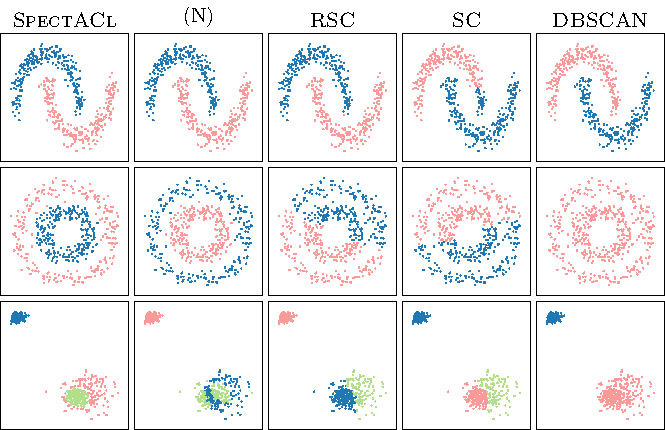
\includegraphics[width=\linewidth]{pics/SASynthScatter.pdf}
%\documentclass[preview=true]{standalone}
\usepackage{amsmath,amssymb,nicefrac,bbm}
\usepackage{pdfathesis}
\usepackage{etex}
\usepackage{xcolor}
\usepackage[a4paper,left=3.5cm,right=2.5cm,bottom=3.5cm,top=3cm]{geometry}
\usepackage[english]{babel}
\usepackage[round]{natbib}
\usepackage{graphicx,tikz}
\usetikzlibrary{matrix,decorations.pathreplacing, calc, positioning}
\usepackage{relsize} % mathlarger
%\usepackage{hyperref,url}
\usepackage{url}
\usepackage{silence}
\WarningFilter{latex}{Overwriting file}

\usepackage[colorinlistoftodos]{todonotes}
\reversemarginpar
\setlength{\marginparwidth}{3.1cm}
% Theorem-Umgebungen
%\usepackage[amsmath,thmmarks]{ntheorem}
\usepackage{amsthm}
\usepackage{thmtools, thm-restate}
\usepackage{algorithm,algpseudocode}
\algnewcommand{\IIf}[1]{\State\algorithmicif\ #1\ \algorithmicthen}
\algnewcommand{\EndIIf}{\unskip\ \algorithmicend\ \algorithmicif}

\usepackage{enumerate}
\usepackage{booktabs,multirow,adjustbox}
\usepackage[font=small,labelfont=bf]{caption}
\usepackage{subfigure}
\usepackage{pgfplots,filecontents,pgfplotstable}
\usepgfplotslibrary{groupplots}
\pgfplotsset{compat=1.14}
\pgfplotsset{
cohStyle/.style={ctrust,mark options ={ctrust},mark repeat={4}, ultra thick, error bars/.cd,y dir = both, y explicit},
densStyle/.style={cdens,dashed,mark options ={cdens},mark repeat={4}, ultra thick, error bars/.cd,y dir = both, y explicit},
primpStyle/.style={cPrimp,dashed,mark=triangle*,mark options ={cPrimp},mark repeat={3}, ultra thick, error bars/.cd,y dir = both, y explicit},
panStyle/.style={cPan,dashed,mark options ={cPan},mark repeat={3}, ultra thick, error bars/.cd,y dir = both, y explicit},
specStyle/.style={cSpec,mark options ={cSpec},mark repeat={4}, thick, error bars/.cd,y dir = both, y explicit},
specLStyle/.style={cSpecL,mark options ={cSpecL},mark repeat={4}, thick, error bars/.cd,y dir = both, y explicit},
RSCStyle/.style={cRSC,dashed,mark=triangle*,mark options ={cRSC},mark repeat={3}, thick, error bars/.cd,y dir = both, y explicit},
SCStyle/.style={cSC,dashed,mark options ={cSC},mark repeat={3}, thick, error bars/.cd,y dir = both, y explicit},
DBSCANStyle/.style={cDBSCAN,dashed,mark options ={cDBSCAN},mark repeat={3}, thick, error bars/.cd,y dir = both, y explicit},
clusterScatterStyle/.style={scatter/classes={1={cSpecL}, 2={cRSC}, 0={cDBSCAN}, -1={white}},
    scatter, only marks, mark size =0.3, scatter src=explicit symbolic},
nonnegScatterStyle/.style={scatter, only marks, fill=cSpec, scatter src=explicit,
     	visualization depends on ={\thisrow{z} \as \perpointmarksize},
     scatter/@pre marker code/.append style={/tikz/mark size=1.5*\perpointmarksize}},
pandaStyle/.style={cPanda,dashed,mark options ={cPanda},mark repeat={3}, ultra thick, error bars/.cd,y dir = both, y explicit},
punkStyle/.style={cPunk,mark options ={cPunk},mark repeat={3}, thick, error bars/.cd,y dir = both, y explicit},
dbssl1Style/.style={cDBSSL1,dashed,mark options ={cDBSSL1},mark=triangle,mark repeat={3}, thick, error bars/.cd,y dir = both, y explicit},
dbssl2Style/.style={cDBSSL2,dashed,mark options ={cDBSSL2},mark=diamond,mark repeat={3}, thick, error bars/.cd,y dir = both, y explicit},
mdlDbsslStyle/.style={cMDLDBSSL,dashed,mark=star,mark options ={cMDLDBSSL},mark repeat={3}, thick, error bars/.cd,y dir = both, y explicit},
% color change for embedding visualization (fuzzy clusters) 
colormap={test}{[2pt]
    rgb255=(166,206,227);
    rgb255=(166,206,227);
},
}

\Title{ A Mathematical Theory of Making Hard Decisions:
Model Selection and Robustness of Matrix Factorization with Binary
Constraints}

%List of Symbols
\usepackage{nomencl}
\makenomenclature


%\usepackage{color}
\definecolor{col1}{RGB}{166,206,227}
\definecolor{col2}{RGB}{31,120,180}
\definecolor{col3}{RGB}{178,223,138}
\definecolor{col4}{RGB}{51,160,44}
\definecolor{col5}{RGB}{251,154,153}
\definecolor{col6}{RGB}{227,26,28}

\definecolor{cdens}{named}{col1}
\definecolor{ctrust}{named}{col2}
\definecolor{cPrimp}{named}{col3}
\definecolor{cPan}{named}{col4}
\definecolor{cPanda}{named}{col5}
\definecolor{cNassau}{named}{col6}
\definecolor{cMdl4bmf}{named}{col1}


%
\definecolor{cSpec}{named}{col1}
\definecolor{cSpecL}{named}{col2}
\definecolor{cRSC}{named}{col3}
\definecolor{cSC}{named}{col4}
\definecolor{cDBSCAN}{named}{col5}

%
\definecolor{cPunk}{named}{col1}
\definecolor{cDBSSL1}{named}{col2}
\definecolor{cDBSSL2}{named}{col4}
\definecolor{cMDLDBSSL}{named}{col5}
% Theorem-Optionen %
%\theoremseparator{.}
%\newenvironment{proof}{\par\noindent{\textit{ Proof}\ }}{\hfill\qed\\[2mm]}
\theoremstyle{plain}
%\theoremheaderfont{\moon}
%\newcommand{\BlackBox}{\rule{1.5ex}{1.5ex}}  % end of proof
%
\newtheorem{theorem}{Theorem}[chapter]
\newtheorem{corollary}[theorem]{Corollary}
\newtheorem{observation}[theorem]{Observation}
\newtheorem{lemma}[theorem]{Lemma}
%\theorembodyfont{\upshape}
\theoremstyle{definition}
\newtheorem{definition}[theorem]{Definition}
\newtheorem{algSpec}{Algorithm Specification}
\newtheorem*{remark}{Remark}
\newtheorem*{example}{Example}
\newtheorem*{problem}{Problem}

%Operators/Commands
\DeclareMathOperator*{\argmin}{arg\,min}
\DeclareMathOperator*{\argmax}{arg\,max}
\DeclareMathOperator*{\freq}{freq}
\DeclareMathOperator*{\cov}{cov}
\DeclareMathOperator*{\anc}{anc}
\DeclareMathOperator*{\supp}{supp}
\DeclareMathOperator*{\minsup}{minsup}
\DeclareMathOperator*{\tr}{tr}
\DeclareMathOperator*{\bigO}{\mathcal{O}}
\DeclareMathOperator{\diag}{diag}
\DeclareMathOperator{\prox}{prox}
\DeclareMathOperator{\pre}{pre}
\DeclareMathOperator{\rec}{rec}
\newcommand{\Ya}{Y_{\mathcal{J}_a\cdot}}
\newcommand{\Va}{{V_a}}
\newcommand{\Da}{D_{\mathcal{J}_a\cdot}}
\newcommand{\KL}{Kurdyka-{\L}ojasiewicz }
\newcommand{\LXU}{\mathcal{L}}
\newcommand{\F}{\mathcal{F}}
\newcommand{\N}{\mathbb{N}}
\newcommand{\R}{\mathbb{R}}
\newcommand{\estU}{\widetilde{U}_{\widehat{CT}}}
\newcommand{\estu}{\tilde{u}_{\widehat{CT}}}
\newcommand{\estCT}{\widehat{CT}}
\newcommand{\node}{\mathfrak{n}}
\newcommand{\leaf}{\mathfrak{t}}
\newcommand{\krimp}{\textsc{Krimp} }
\newcommand{\shrimp}{\textsc{SHrimp} }
\newcommand{\slim}{\textsc{Slim} }

\makeatletter

\pgfplotstableset{
    zero color/.initial=white,
    zero color/.get=\zerocol,
    zero color/.store in=\zerocol,
    one color/.initial=red,
    one color/.get=\onecol,
    one color/.store in=\onecol,
    color cells/.style={
        every head row/.style={output empty row},
        string type,
        postproc cell content/.code={%
           \pgfkeysalso{@cell content=\rule{0cm}{2.4ex}\cellcolor{\zerocol}
           \pgfmathtruncatemacro\number{int(##1)}
           \ifnum\number>100\cellcolor{\onecol!50!black}
           \else \ifnum\number>0\cellcolor{\onecol!##1}\fi\fi}%
        },
        columns/x/.style={
            column name={},
            postproc cell content/.code={}
        }
    }
}
\makeatother

\makeatletter
\newcommand\footnoteref[1]{\protected@xdef\@thefnmark{\ref{#1}}\@footnotemark}
\makeatother

\makeatletter
%\renewcommand{\@chapapp}{}% Not necessary...
\newenvironment{chapquote}[2][2em]
  {\setlength{\@tempdima}{#1}%
   \def\chapquote@author{#2}%
   \parshape 1 \@tempdima \dimexpr\textwidth-2\@tempdima\relax%
   \itshape}
  {\par\normalfont\hfill--\ \chapquote@author\hspace*{\@tempdima}\par\bigskip}
\makeatother

%Thicker bar
\makeatletter
\newcommand{\thickbar}{\mathpalette\@thickbar}
\newcommand{\@thickbar}[2]{{#1\mkern1.5mu\vbox{
  \sbox\z@{$#1\mkern-1.5mu#2\mkern-1.5mu$}%
  \sbox\tw@{$#1\overline{#2}$}%
  \dimen@=\dimexpr\ht\tw@-\ht\z@-.8\p@\relax
  \hrule\@height.8\p@ % adjust for the desired rule thickness
  \vskip\dimen@
  \box\z@}\mkern1.5mu}
}
\makeatother

%----------box---------------
\usepackage[many]{tcolorbox}
\tcbset{
  myhlight/.style={
    colback=cyan!10,
    arc=0pt,
    outer arc=0pt,
    boxrule=0pt,
    top=2pt,
    bottom=2pt,
    left=2pt,
    right=2pt,
  },
  highlight math style={myhlight},
  mybx/.style={
    colback=white,
    arc=0pt,
    outer arc=0pt,
    boxrule=1pt,
    top=2pt,
    bottom=2pt,
    left=2pt,
    right=2pt,
  }
}

\newtcolorbox{mybox}{
	boxsep=1pt,
  	breakable,
  	mybx
}


% Zeilenabstand einstellen %
\renewcommand{\baselinestretch}{1}
% Floating-Umgebungen anpassen %
\renewcommand{\topfraction}{1.0}
\renewcommand{\bottomfraction}{1.0}
\renewcommand{\floatpagefraction}{1.0}
\renewcommand{\dblfloatpagefraction}{1.0}

% Leere Seite ohne Seitennummer, naechste Seite rechts
\newcommand{\blankpage}{
 \clearpage{\pagestyle{empty}\cleardoublepage}
}

% Keine einzelnen Zeilen beim Anfang eines Abschnitts (Schusterjungen)
\clubpenalty = 10000
% Keine einzelnen Zeilen am Ende eines Abschnitts (Hurenkinder)
\widowpenalty = 10000 \displaywidowpenalty = 10000
% EOF
%
\begin{document}
%
\begin{filecontents}{nmSpectACl_eps.dat}
x y z
1.70069743062 2.42758078324 1
0.285683163483 0.820224134154 1
1.96043338205 1.11652004199 1
2.54379828594 0.801796530514 0
1.02584883691 2.57355440485 1
1.93164886191 1.28604223276 1
1.83409801343 1.05168575212 1
1.50665839702 0.598828682981 0
1.21456049586 1.91816830754 0
0.548489010379 2.4266670795 1
2.43718937566 0.259585631612 0
1.08815940258 1.49111722436 0
1.03453098116 1.5879904518 0
0.109412219779 1.28023561758 1
1.9865620235 1.22135031104 1
1.22512830724 1.0225006133 0
2.86565022133 1.80367677252 0
2.89706812992 1.53195814064 0
0.8209715405 1.72041831352 0
0.617806017378 2.40727584262 1
2.28442347034 0.430331423047 0
1.28180236997 1.03358907376 0
0.887937054635 2.68053646933 1
0.891570602061 2.32922789032 1
2.65618201755 0.894877000626 0
0.498394232883 2.45236217747 1
1.35694280656 2.46718908062 1
1.11489573331 1.85699692515 0
2.9080680088 1.73914577833 0
0.785679177354 2.44215259264 1
0.196823873853 1.89256063131 1
1.17823524744 1.75551785493 0
1.23992030311 2.66315904413 1
2.00540849232 0.499253921452 0
0.848956944163 2.45868527982 1
0.0925078051445 1.29305455349 1
0.247138803261 1.95645113223 1
2.83766305835 1.76420767232 0
1.12807120931 1.38527205119 0
1.94201627226 1.40478582163 1
1.25729757329 1.8930319065 0
1.89326303725 1.91932512895 1
1.72383858092 2.21738324713 1
0.45709546568 2.4199525741 1
1.35307081946 2.21860026432 1
1.00887362506 1.94033464961 0
2.34181723671 0.686515872943 0
1.11475444609 0.954182702693 0
0.420448354856 2.32241979328 1
1.59149868632 2.16078316015 1
0.329310350731 1.82923651818 1
0.629423152641 2.36690609361 1
0.307287028638 1.63670049795 1
2.59724264213 0.569519846613 0
0.527392241622 2.54113453641 1
1.91786921713 0.481595165812 0
1.95156790129 2.12611147089 1
1.41194255779 2.66793976628 1
0.0694222959687 1.82183402009 1
1.61367440743 0.544603242775 0
1.84906416078 1.43524726088 1
2.56840153548 0.978613872479 0
2.68782194498 1.60369331079 0
1.6967066369 2.05018333769 1
0.287779916276 1.35181404437 1
2.10581182305 0.58600544124 0
2.76589189346 1.31793021207 0
0.903330891708 2.71981111471 1
1.78910702143 1.78431684787 1
2.85201486168 1.75683049978 0
2.61444426339 1.1421123448 0
1.76686652891 0.412643118932 0
2.38343223857 0.614019382719 0
0.351982420161 1.82124180438 1
1.20104638372 1.08550087193 0
1.71310358783 2.10563588448 1
1.20574320869 1.14241676927 0
1.85476278831 1.68570217527 1
0.866928473775 2.71912423537 1
1.24150157057 1.87008926301 0
1.28290021851 2.54224942198 1
2.20513157208 0.332694252519 0
0.7649274204 2.49776682771 1
1.92833706433 1.74896192577 1
1.12650480957 1.0348913114 0
0.42035554481 2.29433128095 1
1.8227778128 1.73009804176 1
1.40440087482 0.800372448393 0
0.350170029196 1.83113326458 1
2.67833915261 0.955760684365 0
1.45206309833 2.3376423972 1
1.99881809264 0.647288007188 0
1.73930300342 2.27513141315 1
0.997530664835 2.48601880132 1
2.52748209417 0.964779854994 0
0.18616961175 1.41798846544 1
1.27951506157 0.579681303838 0
1.24451979199 1.01467765734 0
1.528155426 0.429507299506 0
1.86116862662 0.0 0
0.229448043123 1.39451828581 1
2.43840791486 0.811277652094 0
1.08024324217 1.45606914327 0
1.69141952321 1.87996999864 1
0.523342152062 2.27879186696 1
2.53685907702 0.842989476903 0
0.781622595306 2.37059793943 1
2.37151355968 0.752368295204 0
1.81585388656 0.405096626174 0
0.526353426641 2.28139242049 1
2.7760661566 0.95760548246 0
0.923603269543 2.64416122336 1
1.94640723913 1.91848140563 1
1.56063634725 2.50248629435 1
1.0176090148 2.72395908515 1
2.31363407826 0.5281707426 0
1.73803401456 1.88934225142 1
0.26732734312 1.01993624365 1
1.92620482073 1.36669614426 1
2.83528847849 2.08551281403 0
1.2560191234 0.92058406981 0
2.38592708362 0.628151589247 0
1.63132977838 0.709002849989 0
1.05904065429 1.51493849809 0
0.139685121871 1.80990844772 1
1.27499215905 1.06475398303 0
1.14937169414 1.42166121091 0
2.33215946967 0.30036289709 0
1.67510627109 0.411176705111 0
1.18231701939 2.50556350357 1
1.77038669418 1.7965018847 1
2.41711258717 1.06425648687 0
1.5466743199 2.19799847606 1
2.81159915284 0.84108084496 0
2.09568775447 0.361760404015 0
1.62856213766 2.40924498166 1
2.39833092966 0.493171096231 0
1.51465143737 2.47271499647 1
1.13635348992 0.947616890809 0
1.04349043595 1.39023226786 0
0.603031169212 2.58849736575 1
1.9387998979 1.22409851527 1
0.128778294394 1.31392528176 1
1.1003283767 1.2661573588 0
0.743838019158 2.52252993124 1
0.61621116068 2.65631385961 1
0.886728816447 2.57220887 1
1.93703048927 0.497335966775 0
1.34132891502 0.890984584948 0
0.536517048738 2.03140735086 1
0.426818260547 2.19895923382 1
0.382225086449 2.24212488028 1
0.90075749994 2.84889611659 1
1.71053267234 0.139893439754 0
1.29639938455 2.59086974776 1
1.94208010739 0.301786108633 0
1.83766716651 1.89862578133 1
0.217910019358 1.18284981176 1
2.87431916031 1.13362681065 0
2.49128297904 0.808660342234 0
0.887367512053 1.77483826418 0
2.41849255062 0.5324350021 0
1.52025137653 2.40917722219 1
2.81144168216 1.32711652029 0
1.04959124228 1.45154913004 0
2.76797402357 1.57360077806 0
1.82169413997 1.6359444949 1
0.463673012107 2.13666946634 1
1.76717691103 0.185518641762 0
1.79700009392 0.415992627791 0
1.07371926343 1.25433471066 0
0.35340797154 2.20777111939 1
0.910470573245 2.57545855259 1
1.00666113925 1.41487472942 0
0.263242311008 2.11420843779 1
1.83750587555 0.960921001284 1
0.598118607947 2.17126465619 1
0.989607517794 2.72016213659 1
0.339991852275 1.6367039174 1
2.81553150588 1.25227670267 0
1.1688157054 1.61925018628 0
2.87702213607 1.62065697172 0
1.18784418709 1.07176694342 0
2.69535677668 1.14397649917 0
2.61215137255 0.908888019432 0
2.2703000471 0.739737480907 0
0.310292767944 1.5927524401 1
1.9751498572 1.39478059397 1
1.05585797661 1.86898397783 0
0.491864333665 2.31875950071 1
2.04280176433 0.227220807369 0
1.29239733899 2.77729312657 1
1.76399564245 0.389462528366 0
1.10987143975 2.45825835483 1
0.888789567782 2.65387087803 1
2.45980643174 0.992909318285 0
1.08897922761 1.42887358233 0
0.759086710455 2.40740216785 1
2.85579700003 1.62503776295 0
1.49047821489 0.578651837622 0
2.14306688802 0.410252695811 0
2.80690341525 1.04739831031 0
1.08084426927 2.37142988192 1
1.24156411616 1.55517287562 0
1.46082893365 0.841033454439 0
1.13147127699 2.53816467841 1
2.47534170514 0.691577879525 0
0.515186721621 2.37712522384 1
0.738658590011 2.23721041569 1
0.152209727518 1.84671174913 1
2.60849673113 0.841526842613 0
1.04231829692 2.71045161422 1
0.964376417508 1.74174356827 0
0.342359603748 2.31301969708 1
0.312328480287 2.0697583552 1
2.45657728683 0.742808305141 0
1.96519472004 1.95521093343 1
0.976026718348 1.65145435908 0
1.70038574297 0.690680548668 0
1.37321471501 0.593617808351 0
1.34431592493 2.38004670142 1
1.20432098055 1.41547092441 0
1.0929063259 1.64510555084 0
1.14149626236 1.27251025565 0
2.38350457204 0.579440777335 0
1.29738017256 2.28865081481 1
1.19200628952 1.85807567095 0
2.29057019712 0.494581835568 0
1.80036719203 2.25739553896 1
1.7374178378 0.17861431239 0
0.681070242517 2.21529849059 1
1.88653779019 1.71753481275 1
1.66130686 0.453575429025 0
1.05708950661 1.30651646662 0
1.7262189757 2.0892030765 1
1.8743608435 1.34263072606 1
1.48620524338 0.715922906298 0
2.00459538411 0.635140423792 0
0.318587109448 1.92679150556 1
1.37843639956 0.707088283144 0
2.60563623353 0.84239504921 0
2.51013047406 1.15186988552 0
1.09765232658 2.56485848597 1
2.65051441579 0.706858112677 0
0.352710453599 1.60528124984 1
1.367034677 2.342617793 1
2.6778340428 1.27583043688 0
2.77041498717 1.62149290572 0
0.433413700012 2.28661466553 1
2.48279234082 0.838028620621 0
0.664103039947 2.61890924636 1
0.485901366946 2.02729851019 1
1.85342076722 0.311040878791 0
2.24141958751 0.69211889508 0
1.05284501061 0.815302813624 0
1.79533297587 1.72925735288 1
1.59592524946 2.291103752 1
1.12311889981 2.73494294316 1
0.239642607379 1.4708710286 1
2.38074908517 0.178741070048 0
1.95942048639 0.485758418579 0
0.801008762883 2.35832224956 1
1.74336065112 2.52814028379 1
2.00425063315 1.44973882129 1
2.99874263731 1.61490975065 0
1.77010542011 2.37104764753 1
1.512850527 2.28856440723 1
2.45235640311 0.561489373791 0
1.295122251 0.789267498929 0
1.51455075898 0.528202376017 0
0.304527789681 1.21175257382 1
1.21559659311 0.781644945741 0
2.13154242053 0.328030655553 0
1.02901463251 1.60574602789 0
1.04967754137 2.46974317694 1
0.383986869727 1.946959298 1
0.674587230211 2.31409008533 1
2.94816733924 1.82970946363 0
1.46163323762 0.792251773345 0
0.660363196201 2.44792160823 1
2.03001716038 0.213480207542 0
1.36368239515 0.799287249057 0
0.100287359104 1.22065856204 1
2.01060150251 0.464874464476 0
2.02983745816 0.305243543361 0
1.2251556746 1.52746937796 0
2.69691681725 1.71441309537 0
2.85609415251 1.41314756677 0
1.01887468848 2.53297875059 1
1.72087173411 1.97290485697 1
0.0540782987346 1.66034457313 1
1.50772484392 0.172194489983 0
1.24910710679 0.732983283934 0
1.21965279462 1.48366422323 0
1.62105492439 2.04589281976 1
2.87108229353 1.48089493044 0
2.86550061675 1.67997945483 0
1.09627892364 1.65438075877 0
0.338132847221 1.79813179713 1
0.436675834273 2.29829461324 1
1.35612302258 0.617635762047 0
2.71578839431 1.11238360205 0
1.84067753076 2.35076159932 1
1.90883244213 1.40654781879 1
0.448930144962 2.42194163441 1
2.27088828505 0.720328288284 0
1.99427584167 0.292469923157 0
2.05179138307 0.075191975576 0
2.75775762337 1.41657699478 0
0.12405803592 1.67542521447 1
2.43818544068 0.725956693576 0
0.312635410658 1.46319738786 1
0.191240314346 1.65611706549 1
2.75529018146 1.51664712917 0
2.87438941247 1.42513159143 0
1.6124710734 0.108162333984 0
2.07748229347 1.37016700533 1
1.34233953375 0.80510418713 0
0.402666931541 1.97206849653 1
1.59991006122 0.430928345538 0
1.76450324322 1.9417972377 1
0.68142574163 2.3657937995 1
0.164887719809 0.933208295559 1
0.917202040984 2.45367836822 1
0.162413262346 1.79806447542 1
1.69954497521 0.474876958658 0
0.885974873525 2.80037127387 1
1.51432134071 2.26982073221 1
1.34621921819 0.906396320943 0
0.691126264848 2.70915758443 1
1.87293313667 1.78727508456 1
2.28649531765 0.726889577091 0
1.07263048888 2.68627388773 1
1.80060022058 0.599304932113 0
1.26924503947 2.54861366445 1
1.05684697644 1.91308852172 0
1.34125453355 0.95711539541 0
2.8125803328 1.52002754851 0
1.21682707227 0.904424035905 0
1.31929933512 2.79201230232 1
0.637404952623 2.32382669843 1
2.17137726399 0.282323068269 0
1.62762538368 2.26290014007 1
0.540666367159 2.33600275939 1
1.88293690233 1.28480350699 1
2.77912006373 1.9726418669 0
0.887955978785 2.55238946452 1
1.85499981106 2.17561046177 1
2.77275743931 1.26672052764 0
1.88408081212 1.55654855145 1
2.20422656878 0.194151609861 0
1.37215670775 0.64239160578 0
2.74173332893 1.06281332167 0
1.3519692899 2.44789629152 1
0.976624716971 1.76062464088 0
1.04508085459 1.58720561346 0
1.86316148119 0.606405006819 0
1.84838679137 0.364768005124 0
0.3387851597 2.31151471375 1
0.695323634969 2.53219749966 1
1.5016800772 2.28286263615 1
1.72601415658 0.425192245283 0
2.7956168279 1.41300555516 0
0.575132420922 2.21555668975 1
1.92736865662 1.30428244235 1
2.86941042658 1.12652831483 0
0.505972295319 2.11848657916 1
2.88083111935 1.79685857086 0
1.54968608895 2.50447888087 1
2.31278971533 0.259675335988 0
2.73879578515 1.18969715242 0
2.41045930274 0.901294611205 0
0.174601175717 1.25065471515 1
2.32186139204 0.515582850319 0
0.20554231582 1.35225498011 1
2.73059185626 1.20383151563 0
1.3865034904 2.53822490098 1
1.12900900657 2.75114078017 1
0.115069738958 1.04596772082 1
1.335120272 2.64619551797 1
0.831696677651 2.37593629365 1
0.292063587839 1.88454278761 1
1.40477301971 2.48630866567 1
0.227853652523 1.72614884781 1
1.39895080992 2.73195382504 1
2.74706816704 1.76622164219 0
1.65483832512 2.04749839106 1
1.9617597714 0.486798653141 0
1.64888491758 2.17115329123 1
1.60586723589 0.501084875631 0
0.284675287626 1.34679532238 1
1.7675237627 2.24242168385 1
1.26193391783 2.60789114088 1
1.85894079362 1.62496524757 1
1.23674367127 0.982304806675 0
1.97582138089 0.509380358308 0
1.05600781745 2.677392365 1
0.184110621272 2.05447883901 1
0.547385160286 2.55233290655 1
2.57887948172 0.828032733195 0
0.207424483914 1.40821380306 1
1.4369592134 2.72855234245 1
1.62259449811 1.74010086385 1
2.672451501 1.6291678069 0
1.81325243451 0.253878981216 0
1.6389068495 2.55396535903 1
1.78009058629 1.82382255609 1
1.82405310361 2.18872776439 1
0.297924979561 2.15608602252 1
0.734938555418 2.43601614007 1
2.76539867309 0.876829399765 0
0.299689834261 2.26240499707 1
0.657100676443 2.54932984854 1
1.97531757625 0.418517119017 0
1.70335971574 2.01957604536 1
2.01136443846 1.56650446432 1
1.9889246753 1.33708935655 1
0.520697457737 2.19392438309 1
0.201610918869 1.11114702728 1
1.18460310214 2.64018309532 1
1.67953679203 2.09096852593 1
2.52903300028 0.668689176375 0
1.82992609123 0.41148308689 0
1.8782077118 1.15964218423 1
2.77296228387 1.32572928549 0
1.82869717065 0.425653875063 0
0.894053475273 2.44439263156 1
1.07621362954 1.70969278243 0
1.45644007418 2.18215955599 1
1.22063523709 1.744321168 0
1.07967091239 1.06274577676 0
1.1900696085 1.26923933736 0
1.04550909582 1.95159439522 0
1.36599613108 0.996983555907 0
1.48939507438 2.55035208922 1
1.39352940488 0.963024804974 0
1.79847337348 1.76745116277 1
2.79775175948 0.989798501929 0
1.85447215813 0.591984136577 0
1.97133310695 1.23755879013 1
1.33548899995 0.903694832059 0
1.24331015073 2.6153250888 1
1.18889713657 2.78378504495 1
0.959819003516 1.85803345242 0
1.48688739481 0.518828000145 0
2.17038326017 0.538678939108 0
2.00401389267 1.2148267132 1
1.80471537631 1.56843402421 1
2.41227229935 0.418729119508 0
1.54810143205 0.592880123322 0
2.70786075559 1.37847478472 0
1.95754047284 1.18045687789 1
0.376516805236 1.88573157828 1
1.55659448472 1.89138211448 1
1.6713666353 0.452084078249 0
2.01552714856 0.493164592727 0
2.92882892778 1.71535055117 0
2.30685921255 0.69876892802 0
0.910811583335 2.47994266873 1
1.20418470115 2.33843955069 1
2.39790481126 0.794684627456 0
2.46701618738 0.581809838238 0
0.251366988518 1.8780274577 1
0.499412691579 2.38088700981 1
2.56205261531 0.65140655269 0
0.421518010626 2.06060390571 1
1.17009887948 1.5134267149 0
2.81288537691 1.68955621988 0
1.85801783879 0.555828770401 0
1.62002253434 2.06714531107 1
0.587232551254 2.47998567591 1
0.929550119504 2.62696249914 1
0.285941297863 1.76825739547 1
0.259015697972 1.26276981669 1
1.90778512029 1.51870006004 1
1.78857330267 0.328932520462 0
1.62111786442 2.21583017128 1
1.55851506264 2.39564830468 1
2.8184718636 1.49831763883 0
1.44366997728 0.811031572419 0
0.670803912622 2.52569944579 1
1.99900347199 1.27336970112 1
1.03545744455 2.67615661925 1
1.94020677429 0.417071861833 0
1.7209951759 0.415479497045 0
2.44397592822 0.627725787503 0
1.38008876818 0.718105733857 0
2.53036245288 0.380380389259 0
1.95319494442 0.992058285038 1
0.983756955407 1.32684250689 0
0.6881145508 2.71837116248 1
1.88019132883 1.60123260018 1
1.29417582527 1.2231395338 0
1.29745287353 2.79297372882 1
0.333622187036 2.26301752448 1
0.32392659893 1.70725807039 1
1.27163496314 2.5038370693 1
0.419549967659 2.16152124321 1
0.70356632396 2.43698318681 1
2.24311863984 0.0606826745953 0
\end{filecontents}
\begin{filecontents}{nmSpectACl_knn_n.dat}
x y z
1.70069743062 2.42758078324 1
0.285683163483 0.820224134154 1
1.96043338205 1.11652004199 1
2.54379828594 0.801796530514 0
1.02584883691 2.57355440485 1
1.93164886191 1.28604223276 1
1.83409801343 1.05168575212 1
1.50665839702 0.598828682981 0
1.21456049586 1.91816830754 0
0.548489010379 2.4266670795 1
2.43718937566 0.259585631612 0
1.08815940258 1.49111722436 0
1.03453098116 1.5879904518 0
0.109412219779 1.28023561758 1
1.9865620235 1.22135031104 1
1.22512830724 1.0225006133 0
2.86565022133 1.80367677252 0
2.89706812992 1.53195814064 0
0.8209715405 1.72041831352 0
0.617806017378 2.40727584262 1
2.28442347034 0.430331423047 0
1.28180236997 1.03358907376 0
0.887937054635 2.68053646933 1
0.891570602061 2.32922789032 1
2.65618201755 0.894877000626 0
0.498394232883 2.45236217747 1
1.35694280656 2.46718908062 1
1.11489573331 1.85699692515 0
2.9080680088 1.73914577833 0
0.785679177354 2.44215259264 1
0.196823873853 1.89256063131 1
1.17823524744 1.75551785493 0
1.23992030311 2.66315904413 1
2.00540849232 0.499253921452 0
0.848956944163 2.45868527982 1
0.0925078051445 1.29305455349 1
0.247138803261 1.95645113223 1
2.83766305835 1.76420767232 0
1.12807120931 1.38527205119 0
1.94201627226 1.40478582163 1
1.25729757329 1.8930319065 0
1.89326303725 1.91932512895 1
1.72383858092 2.21738324713 1
0.45709546568 2.4199525741 1
1.35307081946 2.21860026432 1
1.00887362506 1.94033464961 0
2.34181723671 0.686515872943 0
1.11475444609 0.954182702693 0
0.420448354856 2.32241979328 1
1.59149868632 2.16078316015 1
0.329310350731 1.82923651818 1
0.629423152641 2.36690609361 1
0.307287028638 1.63670049795 1
2.59724264213 0.569519846613 0
0.527392241622 2.54113453641 1
1.91786921713 0.481595165812 0
1.95156790129 2.12611147089 1
1.41194255779 2.66793976628 1
0.0694222959687 1.82183402009 1
1.61367440743 0.544603242775 0
1.84906416078 1.43524726088 1
2.56840153548 0.978613872479 0
2.68782194498 1.60369331079 0
1.6967066369 2.05018333769 1
0.287779916276 1.35181404437 1
2.10581182305 0.58600544124 0
2.76589189346 1.31793021207 0
0.903330891708 2.71981111471 1
1.78910702143 1.78431684787 1
2.85201486168 1.75683049978 0
2.61444426339 1.1421123448 0
1.76686652891 0.412643118932 0
2.38343223857 0.614019382719 0
0.351982420161 1.82124180438 1
1.20104638372 1.08550087193 0
1.71310358783 2.10563588448 1
1.20574320869 1.14241676927 0
1.85476278831 1.68570217527 1
0.866928473775 2.71912423537 1
1.24150157057 1.87008926301 0
1.28290021851 2.54224942198 1
2.20513157208 0.332694252519 0
0.7649274204 2.49776682771 1
1.92833706433 1.74896192577 1
1.12650480957 1.0348913114 0
0.42035554481 2.29433128095 1
1.8227778128 1.73009804176 1
1.40440087482 0.800372448393 0
0.350170029196 1.83113326458 1
2.67833915261 0.955760684365 0
1.45206309833 2.3376423972 1
1.99881809264 0.647288007188 0
1.73930300342 2.27513141315 1
0.997530664835 2.48601880132 1
2.52748209417 0.964779854994 0
0.18616961175 1.41798846544 1
1.27951506157 0.579681303838 0
1.24451979199 1.01467765734 0
1.528155426 0.429507299506 0
1.86116862662 0.0 0
0.229448043123 1.39451828581 1
2.43840791486 0.811277652094 0
1.08024324217 1.45606914327 0
1.69141952321 1.87996999864 1
0.523342152062 2.27879186696 1
2.53685907702 0.842989476903 0
0.781622595306 2.37059793943 1
2.37151355968 0.752368295204 0
1.81585388656 0.405096626174 0
0.526353426641 2.28139242049 1
2.7760661566 0.95760548246 0
0.923603269543 2.64416122336 1
1.94640723913 1.91848140563 1
1.56063634725 2.50248629435 1
1.0176090148 2.72395908515 1
2.31363407826 0.5281707426 0
1.73803401456 1.88934225142 1
0.26732734312 1.01993624365 1
1.92620482073 1.36669614426 1
2.83528847849 2.08551281403 0
1.2560191234 0.92058406981 0
2.38592708362 0.628151589247 0
1.63132977838 0.709002849989 0
1.05904065429 1.51493849809 0
0.139685121871 1.80990844772 1
1.27499215905 1.06475398303 0
1.14937169414 1.42166121091 0
2.33215946967 0.30036289709 0
1.67510627109 0.411176705111 0
1.18231701939 2.50556350357 1
1.77038669418 1.7965018847 1
2.41711258717 1.06425648687 0
1.5466743199 2.19799847606 1
2.81159915284 0.84108084496 0
2.09568775447 0.361760404015 0
1.62856213766 2.40924498166 1
2.39833092966 0.493171096231 0
1.51465143737 2.47271499647 1
1.13635348992 0.947616890809 0
1.04349043595 1.39023226786 0
0.603031169212 2.58849736575 1
1.9387998979 1.22409851527 1
0.128778294394 1.31392528176 1
1.1003283767 1.2661573588 0
0.743838019158 2.52252993124 1
0.61621116068 2.65631385961 1
0.886728816447 2.57220887 1
1.93703048927 0.497335966775 0
1.34132891502 0.890984584948 0
0.536517048738 2.03140735086 1
0.426818260547 2.19895923382 1
0.382225086449 2.24212488028 1
0.90075749994 2.84889611659 1
1.71053267234 0.139893439754 0
1.29639938455 2.59086974776 1
1.94208010739 0.301786108633 0
1.83766716651 1.89862578133 1
0.217910019358 1.18284981176 1
2.87431916031 1.13362681065 0
2.49128297904 0.808660342234 0
0.887367512053 1.77483826418 0
2.41849255062 0.5324350021 0
1.52025137653 2.40917722219 1
2.81144168216 1.32711652029 0
1.04959124228 1.45154913004 0
2.76797402357 1.57360077806 0
1.82169413997 1.6359444949 1
0.463673012107 2.13666946634 1
1.76717691103 0.185518641762 0
1.79700009392 0.415992627791 0
1.07371926343 1.25433471066 0
0.35340797154 2.20777111939 1
0.910470573245 2.57545855259 1
1.00666113925 1.41487472942 0
0.263242311008 2.11420843779 1
1.83750587555 0.960921001284 1
0.598118607947 2.17126465619 1
0.989607517794 2.72016213659 1
0.339991852275 1.6367039174 1
2.81553150588 1.25227670267 0
1.1688157054 1.61925018628 0
2.87702213607 1.62065697172 0
1.18784418709 1.07176694342 0
2.69535677668 1.14397649917 0
2.61215137255 0.908888019432 0
2.2703000471 0.739737480907 0
0.310292767944 1.5927524401 1
1.9751498572 1.39478059397 1
1.05585797661 1.86898397783 0
0.491864333665 2.31875950071 1
2.04280176433 0.227220807369 0
1.29239733899 2.77729312657 1
1.76399564245 0.389462528366 0
1.10987143975 2.45825835483 1
0.888789567782 2.65387087803 1
2.45980643174 0.992909318285 0
1.08897922761 1.42887358233 0
0.759086710455 2.40740216785 1
2.85579700003 1.62503776295 0
1.49047821489 0.578651837622 0
2.14306688802 0.410252695811 0
2.80690341525 1.04739831031 0
1.08084426927 2.37142988192 1
1.24156411616 1.55517287562 0
1.46082893365 0.841033454439 0
1.13147127699 2.53816467841 1
2.47534170514 0.691577879525 0
0.515186721621 2.37712522384 1
0.738658590011 2.23721041569 1
0.152209727518 1.84671174913 1
2.60849673113 0.841526842613 0
1.04231829692 2.71045161422 1
0.964376417508 1.74174356827 0
0.342359603748 2.31301969708 1
0.312328480287 2.0697583552 1
2.45657728683 0.742808305141 0
1.96519472004 1.95521093343 1
0.976026718348 1.65145435908 0
1.70038574297 0.690680548668 0
1.37321471501 0.593617808351 0
1.34431592493 2.38004670142 1
1.20432098055 1.41547092441 0
1.0929063259 1.64510555084 0
1.14149626236 1.27251025565 0
2.38350457204 0.579440777335 0
1.29738017256 2.28865081481 1
1.19200628952 1.85807567095 0
2.29057019712 0.494581835568 0
1.80036719203 2.25739553896 1
1.7374178378 0.17861431239 0
0.681070242517 2.21529849059 1
1.88653779019 1.71753481275 1
1.66130686 0.453575429025 0
1.05708950661 1.30651646662 0
1.7262189757 2.0892030765 1
1.8743608435 1.34263072606 1
1.48620524338 0.715922906298 0
2.00459538411 0.635140423792 0
0.318587109448 1.92679150556 1
1.37843639956 0.707088283144 0
2.60563623353 0.84239504921 0
2.51013047406 1.15186988552 0
1.09765232658 2.56485848597 1
2.65051441579 0.706858112677 0
0.352710453599 1.60528124984 1
1.367034677 2.342617793 1
2.6778340428 1.27583043688 0
2.77041498717 1.62149290572 0
0.433413700012 2.28661466553 1
2.48279234082 0.838028620621 0
0.664103039947 2.61890924636 1
0.485901366946 2.02729851019 1
1.85342076722 0.311040878791 0
2.24141958751 0.69211889508 0
1.05284501061 0.815302813624 0
1.79533297587 1.72925735288 1
1.59592524946 2.291103752 1
1.12311889981 2.73494294316 1
0.239642607379 1.4708710286 1
2.38074908517 0.178741070048 0
1.95942048639 0.485758418579 0
0.801008762883 2.35832224956 1
1.74336065112 2.52814028379 1
2.00425063315 1.44973882129 1
2.99874263731 1.61490975065 0
1.77010542011 2.37104764753 1
1.512850527 2.28856440723 1
2.45235640311 0.561489373791 0
1.295122251 0.789267498929 0
1.51455075898 0.528202376017 0
0.304527789681 1.21175257382 1
1.21559659311 0.781644945741 0
2.13154242053 0.328030655553 0
1.02901463251 1.60574602789 0
1.04967754137 2.46974317694 1
0.383986869727 1.946959298 1
0.674587230211 2.31409008533 1
2.94816733924 1.82970946363 0
1.46163323762 0.792251773345 0
0.660363196201 2.44792160823 1
2.03001716038 0.213480207542 0
1.36368239515 0.799287249057 0
0.100287359104 1.22065856204 1
2.01060150251 0.464874464476 0
2.02983745816 0.305243543361 0
1.2251556746 1.52746937796 0
2.69691681725 1.71441309537 0
2.85609415251 1.41314756677 0
1.01887468848 2.53297875059 1
1.72087173411 1.97290485697 1
0.0540782987346 1.66034457313 1
1.50772484392 0.172194489983 0
1.24910710679 0.732983283934 0
1.21965279462 1.48366422323 0
1.62105492439 2.04589281976 1
2.87108229353 1.48089493044 0
2.86550061675 1.67997945483 0
1.09627892364 1.65438075877 0
0.338132847221 1.79813179713 1
0.436675834273 2.29829461324 1
1.35612302258 0.617635762047 0
2.71578839431 1.11238360205 0
1.84067753076 2.35076159932 1
1.90883244213 1.40654781879 1
0.448930144962 2.42194163441 1
2.27088828505 0.720328288284 0
1.99427584167 0.292469923157 0
2.05179138307 0.075191975576 0
2.75775762337 1.41657699478 0
0.12405803592 1.67542521447 1
2.43818544068 0.725956693576 0
0.312635410658 1.46319738786 1
0.191240314346 1.65611706549 1
2.75529018146 1.51664712917 0
2.87438941247 1.42513159143 0
1.6124710734 0.108162333984 0
2.07748229347 1.37016700533 1
1.34233953375 0.80510418713 0
0.402666931541 1.97206849653 1
1.59991006122 0.430928345538 0
1.76450324322 1.9417972377 1
0.68142574163 2.3657937995 1
0.164887719809 0.933208295559 1
0.917202040984 2.45367836822 1
0.162413262346 1.79806447542 1
1.69954497521 0.474876958658 0
0.885974873525 2.80037127387 1
1.51432134071 2.26982073221 1
1.34621921819 0.906396320943 0
0.691126264848 2.70915758443 1
1.87293313667 1.78727508456 1
2.28649531765 0.726889577091 0
1.07263048888 2.68627388773 1
1.80060022058 0.599304932113 0
1.26924503947 2.54861366445 1
1.05684697644 1.91308852172 0
1.34125453355 0.95711539541 0
2.8125803328 1.52002754851 0
1.21682707227 0.904424035905 0
1.31929933512 2.79201230232 1
0.637404952623 2.32382669843 1
2.17137726399 0.282323068269 0
1.62762538368 2.26290014007 1
0.540666367159 2.33600275939 1
1.88293690233 1.28480350699 1
2.77912006373 1.9726418669 0
0.887955978785 2.55238946452 1
1.85499981106 2.17561046177 1
2.77275743931 1.26672052764 0
1.88408081212 1.55654855145 1
2.20422656878 0.194151609861 0
1.37215670775 0.64239160578 0
2.74173332893 1.06281332167 0
1.3519692899 2.44789629152 1
0.976624716971 1.76062464088 0
1.04508085459 1.58720561346 0
1.86316148119 0.606405006819 0
1.84838679137 0.364768005124 0
0.3387851597 2.31151471375 1
0.695323634969 2.53219749966 1
1.5016800772 2.28286263615 1
1.72601415658 0.425192245283 0
2.7956168279 1.41300555516 0
0.575132420922 2.21555668975 1
1.92736865662 1.30428244235 1
2.86941042658 1.12652831483 0
0.505972295319 2.11848657916 1
2.88083111935 1.79685857086 0
1.54968608895 2.50447888087 1
2.31278971533 0.259675335988 0
2.73879578515 1.18969715242 0
2.41045930274 0.901294611205 0
0.174601175717 1.25065471515 1
2.32186139204 0.515582850319 0
0.20554231582 1.35225498011 1
2.73059185626 1.20383151563 0
1.3865034904 2.53822490098 1
1.12900900657 2.75114078017 1
0.115069738958 1.04596772082 1
1.335120272 2.64619551797 1
0.831696677651 2.37593629365 1
0.292063587839 1.88454278761 1
1.40477301971 2.48630866567 1
0.227853652523 1.72614884781 1
1.39895080992 2.73195382504 1
2.74706816704 1.76622164219 0
1.65483832512 2.04749839106 1
1.9617597714 0.486798653141 0
1.64888491758 2.17115329123 1
1.60586723589 0.501084875631 0
0.284675287626 1.34679532238 1
1.7675237627 2.24242168385 1
1.26193391783 2.60789114088 1
1.85894079362 1.62496524757 1
1.23674367127 0.982304806675 0
1.97582138089 0.509380358308 0
1.05600781745 2.677392365 1
0.184110621272 2.05447883901 1
0.547385160286 2.55233290655 1
2.57887948172 0.828032733195 0
0.207424483914 1.40821380306 1
1.4369592134 2.72855234245 1
1.62259449811 1.74010086385 1
2.672451501 1.6291678069 0
1.81325243451 0.253878981216 0
1.6389068495 2.55396535903 1
1.78009058629 1.82382255609 1
1.82405310361 2.18872776439 1
0.297924979561 2.15608602252 1
0.734938555418 2.43601614007 1
2.76539867309 0.876829399765 0
0.299689834261 2.26240499707 1
0.657100676443 2.54932984854 1
1.97531757625 0.418517119017 0
1.70335971574 2.01957604536 1
2.01136443846 1.56650446432 1
1.9889246753 1.33708935655 1
0.520697457737 2.19392438309 1
0.201610918869 1.11114702728 1
1.18460310214 2.64018309532 1
1.67953679203 2.09096852593 1
2.52903300028 0.668689176375 0
1.82992609123 0.41148308689 0
1.8782077118 1.15964218423 1
2.77296228387 1.32572928549 0
1.82869717065 0.425653875063 0
0.894053475273 2.44439263156 1
1.07621362954 1.70969278243 0
1.45644007418 2.18215955599 1
1.22063523709 1.744321168 0
1.07967091239 1.06274577676 0
1.1900696085 1.26923933736 0
1.04550909582 1.95159439522 0
1.36599613108 0.996983555907 0
1.48939507438 2.55035208922 1
1.39352940488 0.963024804974 0
1.79847337348 1.76745116277 1
2.79775175948 0.989798501929 0
1.85447215813 0.591984136577 0
1.97133310695 1.23755879013 1
1.33548899995 0.903694832059 0
1.24331015073 2.6153250888 1
1.18889713657 2.78378504495 1
0.959819003516 1.85803345242 0
1.48688739481 0.518828000145 0
2.17038326017 0.538678939108 0
2.00401389267 1.2148267132 1
1.80471537631 1.56843402421 1
2.41227229935 0.418729119508 0
1.54810143205 0.592880123322 0
2.70786075559 1.37847478472 0
1.95754047284 1.18045687789 1
0.376516805236 1.88573157828 1
1.55659448472 1.89138211448 1
1.6713666353 0.452084078249 0
2.01552714856 0.493164592727 0
2.92882892778 1.71535055117 0
2.30685921255 0.69876892802 0
0.910811583335 2.47994266873 1
1.20418470115 2.33843955069 1
2.39790481126 0.794684627456 0
2.46701618738 0.581809838238 0
0.251366988518 1.8780274577 1
0.499412691579 2.38088700981 1
2.56205261531 0.65140655269 0
0.421518010626 2.06060390571 1
1.17009887948 1.5134267149 0
2.81288537691 1.68955621988 0
1.85801783879 0.555828770401 0
1.62002253434 2.06714531107 1
0.587232551254 2.47998567591 1
0.929550119504 2.62696249914 1
0.285941297863 1.76825739547 1
0.259015697972 1.26276981669 1
1.90778512029 1.51870006004 1
1.78857330267 0.328932520462 0
1.62111786442 2.21583017128 1
1.55851506264 2.39564830468 1
2.8184718636 1.49831763883 0
1.44366997728 0.811031572419 0
0.670803912622 2.52569944579 1
1.99900347199 1.27336970112 1
1.03545744455 2.67615661925 1
1.94020677429 0.417071861833 0
1.7209951759 0.415479497045 0
2.44397592822 0.627725787503 0
1.38008876818 0.718105733857 0
2.53036245288 0.380380389259 0
1.95319494442 0.992058285038 1
0.983756955407 1.32684250689 0
0.6881145508 2.71837116248 1
1.88019132883 1.60123260018 1
1.29417582527 1.2231395338 0
1.29745287353 2.79297372882 1
0.333622187036 2.26301752448 1
0.32392659893 1.70725807039 1
1.27163496314 2.5038370693 1
0.419549967659 2.16152124321 1
0.70356632396 2.43698318681 1
2.24311863984 0.0606826745953 0
\end{filecontents}
\begin{filecontents}{nmSC_knn_n.dat}
x y z
1.70069743062 2.42758078324 0
0.285683163483 0.820224134154 0
1.96043338205 1.11652004199 1
2.54379828594 0.801796530514 1
1.02584883691 2.57355440485 0
1.93164886191 1.28604223276 1
1.83409801343 1.05168575212 1
1.50665839702 0.598828682981 1
1.21456049586 1.91816830754 1
0.548489010379 2.4266670795 0
2.43718937566 0.259585631612 1
1.08815940258 1.49111722436 1
1.03453098116 1.5879904518 1
0.109412219779 1.28023561758 0
1.9865620235 1.22135031104 1
1.22512830724 1.0225006133 1
2.86565022133 1.80367677252 1
2.89706812992 1.53195814064 1
0.8209715405 1.72041831352 1
0.617806017378 2.40727584262 0
2.28442347034 0.430331423047 1
1.28180236997 1.03358907376 1
0.887937054635 2.68053646933 0
0.891570602061 2.32922789032 0
2.65618201755 0.894877000626 1
0.498394232883 2.45236217747 0
1.35694280656 2.46718908062 0
1.11489573331 1.85699692515 1
2.9080680088 1.73914577833 1
0.785679177354 2.44215259264 0
0.196823873853 1.89256063131 0
1.17823524744 1.75551785493 1
1.23992030311 2.66315904413 0
2.00540849232 0.499253921452 1
0.848956944163 2.45868527982 0
0.0925078051445 1.29305455349 0
0.247138803261 1.95645113223 0
2.83766305835 1.76420767232 1
1.12807120931 1.38527205119 1
1.94201627226 1.40478582163 1
1.25729757329 1.8930319065 1
1.89326303725 1.91932512895 0
1.72383858092 2.21738324713 0
0.45709546568 2.4199525741 0
1.35307081946 2.21860026432 0
1.00887362506 1.94033464961 1
2.34181723671 0.686515872943 1
1.11475444609 0.954182702693 1
0.420448354856 2.32241979328 0
1.59149868632 2.16078316015 0
0.329310350731 1.82923651818 0
0.629423152641 2.36690609361 0
0.307287028638 1.63670049795 0
2.59724264213 0.569519846613 1
0.527392241622 2.54113453641 0
1.91786921713 0.481595165812 1
1.95156790129 2.12611147089 0
1.41194255779 2.66793976628 0
0.0694222959687 1.82183402009 0
1.61367440743 0.544603242775 1
1.84906416078 1.43524726088 1
2.56840153548 0.978613872479 1
2.68782194498 1.60369331079 1
1.6967066369 2.05018333769 0
0.287779916276 1.35181404437 0
2.10581182305 0.58600544124 1
2.76589189346 1.31793021207 1
0.903330891708 2.71981111471 0
1.78910702143 1.78431684787 0
2.85201486168 1.75683049978 1
2.61444426339 1.1421123448 1
1.76686652891 0.412643118932 1
2.38343223857 0.614019382719 1
0.351982420161 1.82124180438 0
1.20104638372 1.08550087193 1
1.71310358783 2.10563588448 0
1.20574320869 1.14241676927 1
1.85476278831 1.68570217527 1
0.866928473775 2.71912423537 0
1.24150157057 1.87008926301 1
1.28290021851 2.54224942198 0
2.20513157208 0.332694252519 1
0.7649274204 2.49776682771 0
1.92833706433 1.74896192577 0
1.12650480957 1.0348913114 1
0.42035554481 2.29433128095 0
1.8227778128 1.73009804176 0
1.40440087482 0.800372448393 1
0.350170029196 1.83113326458 0
2.67833915261 0.955760684365 1
1.45206309833 2.3376423972 0
1.99881809264 0.647288007188 1
1.73930300342 2.27513141315 0
0.997530664835 2.48601880132 0
2.52748209417 0.964779854994 1
0.18616961175 1.41798846544 0
1.27951506157 0.579681303838 1
1.24451979199 1.01467765734 1
1.528155426 0.429507299506 1
1.86116862662 0.0 1
0.229448043123 1.39451828581 0
2.43840791486 0.811277652094 1
1.08024324217 1.45606914327 1
1.69141952321 1.87996999864 0
0.523342152062 2.27879186696 0
2.53685907702 0.842989476903 1
0.781622595306 2.37059793943 0
2.37151355968 0.752368295204 1
1.81585388656 0.405096626174 1
0.526353426641 2.28139242049 0
2.7760661566 0.95760548246 1
0.923603269543 2.64416122336 0
1.94640723913 1.91848140563 0
1.56063634725 2.50248629435 0
1.0176090148 2.72395908515 0
2.31363407826 0.5281707426 1
1.73803401456 1.88934225142 0
0.26732734312 1.01993624365 0
1.92620482073 1.36669614426 1
2.83528847849 2.08551281403 1
1.2560191234 0.92058406981 1
2.38592708362 0.628151589247 1
1.63132977838 0.709002849989 1
1.05904065429 1.51493849809 1
0.139685121871 1.80990844772 0
1.27499215905 1.06475398303 1
1.14937169414 1.42166121091 1
2.33215946967 0.30036289709 1
1.67510627109 0.411176705111 1
1.18231701939 2.50556350357 0
1.77038669418 1.7965018847 0
2.41711258717 1.06425648687 1
1.5466743199 2.19799847606 0
2.81159915284 0.84108084496 1
2.09568775447 0.361760404015 1
1.62856213766 2.40924498166 0
2.39833092966 0.493171096231 1
1.51465143737 2.47271499647 0
1.13635348992 0.947616890809 1
1.04349043595 1.39023226786 1
0.603031169212 2.58849736575 0
1.9387998979 1.22409851527 1
0.128778294394 1.31392528176 0
1.1003283767 1.2661573588 1
0.743838019158 2.52252993124 0
0.61621116068 2.65631385961 0
0.886728816447 2.57220887 0
1.93703048927 0.497335966775 1
1.34132891502 0.890984584948 1
0.536517048738 2.03140735086 0
0.426818260547 2.19895923382 0
0.382225086449 2.24212488028 0
0.90075749994 2.84889611659 0
1.71053267234 0.139893439754 1
1.29639938455 2.59086974776 0
1.94208010739 0.301786108633 1
1.83766716651 1.89862578133 0
0.217910019358 1.18284981176 0
2.87431916031 1.13362681065 1
2.49128297904 0.808660342234 1
0.887367512053 1.77483826418 1
2.41849255062 0.5324350021 1
1.52025137653 2.40917722219 0
2.81144168216 1.32711652029 1
1.04959124228 1.45154913004 1
2.76797402357 1.57360077806 1
1.82169413997 1.6359444949 1
0.463673012107 2.13666946634 0
1.76717691103 0.185518641762 1
1.79700009392 0.415992627791 1
1.07371926343 1.25433471066 1
0.35340797154 2.20777111939 0
0.910470573245 2.57545855259 0
1.00666113925 1.41487472942 1
0.263242311008 2.11420843779 0
1.83750587555 0.960921001284 1
0.598118607947 2.17126465619 0
0.989607517794 2.72016213659 0
0.339991852275 1.6367039174 0
2.81553150588 1.25227670267 1
1.1688157054 1.61925018628 1
2.87702213607 1.62065697172 1
1.18784418709 1.07176694342 1
2.69535677668 1.14397649917 1
2.61215137255 0.908888019432 1
2.2703000471 0.739737480907 1
0.310292767944 1.5927524401 0
1.9751498572 1.39478059397 1
1.05585797661 1.86898397783 1
0.491864333665 2.31875950071 0
2.04280176433 0.227220807369 1
1.29239733899 2.77729312657 0
1.76399564245 0.389462528366 1
1.10987143975 2.45825835483 0
0.888789567782 2.65387087803 0
2.45980643174 0.992909318285 1
1.08897922761 1.42887358233 1
0.759086710455 2.40740216785 0
2.85579700003 1.62503776295 1
1.49047821489 0.578651837622 1
2.14306688802 0.410252695811 1
2.80690341525 1.04739831031 1
1.08084426927 2.37142988192 0
1.24156411616 1.55517287562 1
1.46082893365 0.841033454439 1
1.13147127699 2.53816467841 0
2.47534170514 0.691577879525 1
0.515186721621 2.37712522384 0
0.738658590011 2.23721041569 0
0.152209727518 1.84671174913 0
2.60849673113 0.841526842613 1
1.04231829692 2.71045161422 0
0.964376417508 1.74174356827 1
0.342359603748 2.31301969708 0
0.312328480287 2.0697583552 0
2.45657728683 0.742808305141 1
1.96519472004 1.95521093343 0
0.976026718348 1.65145435908 1
1.70038574297 0.690680548668 1
1.37321471501 0.593617808351 1
1.34431592493 2.38004670142 0
1.20432098055 1.41547092441 1
1.0929063259 1.64510555084 1
1.14149626236 1.27251025565 1
2.38350457204 0.579440777335 1
1.29738017256 2.28865081481 0
1.19200628952 1.85807567095 1
2.29057019712 0.494581835568 1
1.80036719203 2.25739553896 0
1.7374178378 0.17861431239 1
0.681070242517 2.21529849059 0
1.88653779019 1.71753481275 0
1.66130686 0.453575429025 1
1.05708950661 1.30651646662 1
1.7262189757 2.0892030765 0
1.8743608435 1.34263072606 1
1.48620524338 0.715922906298 1
2.00459538411 0.635140423792 1
0.318587109448 1.92679150556 0
1.37843639956 0.707088283144 1
2.60563623353 0.84239504921 1
2.51013047406 1.15186988552 1
1.09765232658 2.56485848597 0
2.65051441579 0.706858112677 1
0.352710453599 1.60528124984 0
1.367034677 2.342617793 0
2.6778340428 1.27583043688 1
2.77041498717 1.62149290572 1
0.433413700012 2.28661466553 0
2.48279234082 0.838028620621 1
0.664103039947 2.61890924636 0
0.485901366946 2.02729851019 0
1.85342076722 0.311040878791 1
2.24141958751 0.69211889508 1
1.05284501061 0.815302813624 1
1.79533297587 1.72925735288 0
1.59592524946 2.291103752 0
1.12311889981 2.73494294316 0
0.239642607379 1.4708710286 0
2.38074908517 0.178741070048 1
1.95942048639 0.485758418579 1
0.801008762883 2.35832224956 0
1.74336065112 2.52814028379 0
2.00425063315 1.44973882129 1
2.99874263731 1.61490975065 1
1.77010542011 2.37104764753 0
1.512850527 2.28856440723 0
2.45235640311 0.561489373791 1
1.295122251 0.789267498929 1
1.51455075898 0.528202376017 1
0.304527789681 1.21175257382 0
1.21559659311 0.781644945741 1
2.13154242053 0.328030655553 1
1.02901463251 1.60574602789 1
1.04967754137 2.46974317694 0
0.383986869727 1.946959298 0
0.674587230211 2.31409008533 0
2.94816733924 1.82970946363 1
1.46163323762 0.792251773345 1
0.660363196201 2.44792160823 0
2.03001716038 0.213480207542 1
1.36368239515 0.799287249057 1
0.100287359104 1.22065856204 0
2.01060150251 0.464874464476 1
2.02983745816 0.305243543361 1
1.2251556746 1.52746937796 1
2.69691681725 1.71441309537 1
2.85609415251 1.41314756677 1
1.01887468848 2.53297875059 0
1.72087173411 1.97290485697 0
0.0540782987346 1.66034457313 0
1.50772484392 0.172194489983 1
1.24910710679 0.732983283934 1
1.21965279462 1.48366422323 1
1.62105492439 2.04589281976 0
2.87108229353 1.48089493044 1
2.86550061675 1.67997945483 1
1.09627892364 1.65438075877 1
0.338132847221 1.79813179713 0
0.436675834273 2.29829461324 0
1.35612302258 0.617635762047 1
2.71578839431 1.11238360205 1
1.84067753076 2.35076159932 0
1.90883244213 1.40654781879 1
0.448930144962 2.42194163441 0
2.27088828505 0.720328288284 1
1.99427584167 0.292469923157 1
2.05179138307 0.075191975576 1
2.75775762337 1.41657699478 1
0.12405803592 1.67542521447 0
2.43818544068 0.725956693576 1
0.312635410658 1.46319738786 0
0.191240314346 1.65611706549 0
2.75529018146 1.51664712917 1
2.87438941247 1.42513159143 1
1.6124710734 0.108162333984 1
2.07748229347 1.37016700533 1
1.34233953375 0.80510418713 1
0.402666931541 1.97206849653 0
1.59991006122 0.430928345538 1
1.76450324322 1.9417972377 0
0.68142574163 2.3657937995 0
0.164887719809 0.933208295559 0
0.917202040984 2.45367836822 0
0.162413262346 1.79806447542 0
1.69954497521 0.474876958658 1
0.885974873525 2.80037127387 0
1.51432134071 2.26982073221 0
1.34621921819 0.906396320943 1
0.691126264848 2.70915758443 0
1.87293313667 1.78727508456 0
2.28649531765 0.726889577091 1
1.07263048888 2.68627388773 0
1.80060022058 0.599304932113 1
1.26924503947 2.54861366445 0
1.05684697644 1.91308852172 1
1.34125453355 0.95711539541 1
2.8125803328 1.52002754851 1
1.21682707227 0.904424035905 1
1.31929933512 2.79201230232 0
0.637404952623 2.32382669843 0
2.17137726399 0.282323068269 1
1.62762538368 2.26290014007 0
0.540666367159 2.33600275939 0
1.88293690233 1.28480350699 1
2.77912006373 1.9726418669 1
0.887955978785 2.55238946452 0
1.85499981106 2.17561046177 0
2.77275743931 1.26672052764 1
1.88408081212 1.55654855145 1
2.20422656878 0.194151609861 1
1.37215670775 0.64239160578 1
2.74173332893 1.06281332167 1
1.3519692899 2.44789629152 0
0.976624716971 1.76062464088 1
1.04508085459 1.58720561346 1
1.86316148119 0.606405006819 1
1.84838679137 0.364768005124 1
0.3387851597 2.31151471375 0
0.695323634969 2.53219749966 0
1.5016800772 2.28286263615 0
1.72601415658 0.425192245283 1
2.7956168279 1.41300555516 1
0.575132420922 2.21555668975 0
1.92736865662 1.30428244235 1
2.86941042658 1.12652831483 1
0.505972295319 2.11848657916 0
2.88083111935 1.79685857086 1
1.54968608895 2.50447888087 0
2.31278971533 0.259675335988 1
2.73879578515 1.18969715242 1
2.41045930274 0.901294611205 1
0.174601175717 1.25065471515 0
2.32186139204 0.515582850319 1
0.20554231582 1.35225498011 0
2.73059185626 1.20383151563 1
1.3865034904 2.53822490098 0
1.12900900657 2.75114078017 0
0.115069738958 1.04596772082 0
1.335120272 2.64619551797 0
0.831696677651 2.37593629365 0
0.292063587839 1.88454278761 0
1.40477301971 2.48630866567 0
0.227853652523 1.72614884781 0
1.39895080992 2.73195382504 0
2.74706816704 1.76622164219 1
1.65483832512 2.04749839106 0
1.9617597714 0.486798653141 1
1.64888491758 2.17115329123 0
1.60586723589 0.501084875631 1
0.284675287626 1.34679532238 0
1.7675237627 2.24242168385 0
1.26193391783 2.60789114088 0
1.85894079362 1.62496524757 1
1.23674367127 0.982304806675 1
1.97582138089 0.509380358308 1
1.05600781745 2.677392365 0
0.184110621272 2.05447883901 0
0.547385160286 2.55233290655 0
2.57887948172 0.828032733195 1
0.207424483914 1.40821380306 0
1.4369592134 2.72855234245 0
1.62259449811 1.74010086385 0
2.672451501 1.6291678069 1
1.81325243451 0.253878981216 1
1.6389068495 2.55396535903 0
1.78009058629 1.82382255609 0
1.82405310361 2.18872776439 0
0.297924979561 2.15608602252 0
0.734938555418 2.43601614007 0
2.76539867309 0.876829399765 1
0.299689834261 2.26240499707 0
0.657100676443 2.54932984854 0
1.97531757625 0.418517119017 1
1.70335971574 2.01957604536 0
2.01136443846 1.56650446432 1
1.9889246753 1.33708935655 1
0.520697457737 2.19392438309 0
0.201610918869 1.11114702728 0
1.18460310214 2.64018309532 0
1.67953679203 2.09096852593 0
2.52903300028 0.668689176375 1
1.82992609123 0.41148308689 1
1.8782077118 1.15964218423 1
2.77296228387 1.32572928549 1
1.82869717065 0.425653875063 1
0.894053475273 2.44439263156 0
1.07621362954 1.70969278243 1
1.45644007418 2.18215955599 0
1.22063523709 1.744321168 1
1.07967091239 1.06274577676 1
1.1900696085 1.26923933736 1
1.04550909582 1.95159439522 1
1.36599613108 0.996983555907 1
1.48939507438 2.55035208922 0
1.39352940488 0.963024804974 1
1.79847337348 1.76745116277 0
2.79775175948 0.989798501929 1
1.85447215813 0.591984136577 1
1.97133310695 1.23755879013 1
1.33548899995 0.903694832059 1
1.24331015073 2.6153250888 0
1.18889713657 2.78378504495 0
0.959819003516 1.85803345242 1
1.48688739481 0.518828000145 1
2.17038326017 0.538678939108 1
2.00401389267 1.2148267132 1
1.80471537631 1.56843402421 1
2.41227229935 0.418729119508 1
1.54810143205 0.592880123322 1
2.70786075559 1.37847478472 1
1.95754047284 1.18045687789 1
0.376516805236 1.88573157828 0
1.55659448472 1.89138211448 0
1.6713666353 0.452084078249 1
2.01552714856 0.493164592727 1
2.92882892778 1.71535055117 1
2.30685921255 0.69876892802 1
0.910811583335 2.47994266873 0
1.20418470115 2.33843955069 0
2.39790481126 0.794684627456 1
2.46701618738 0.581809838238 1
0.251366988518 1.8780274577 0
0.499412691579 2.38088700981 0
2.56205261531 0.65140655269 1
0.421518010626 2.06060390571 0
1.17009887948 1.5134267149 1
2.81288537691 1.68955621988 1
1.85801783879 0.555828770401 1
1.62002253434 2.06714531107 0
0.587232551254 2.47998567591 0
0.929550119504 2.62696249914 0
0.285941297863 1.76825739547 0
0.259015697972 1.26276981669 0
1.90778512029 1.51870006004 1
1.78857330267 0.328932520462 1
1.62111786442 2.21583017128 0
1.55851506264 2.39564830468 0
2.8184718636 1.49831763883 1
1.44366997728 0.811031572419 1
0.670803912622 2.52569944579 0
1.99900347199 1.27336970112 1
1.03545744455 2.67615661925 0
1.94020677429 0.417071861833 1
1.7209951759 0.415479497045 1
2.44397592822 0.627725787503 1
1.38008876818 0.718105733857 1
2.53036245288 0.380380389259 1
1.95319494442 0.992058285038 1
0.983756955407 1.32684250689 1
0.6881145508 2.71837116248 0
1.88019132883 1.60123260018 1
1.29417582527 1.2231395338 1
1.29745287353 2.79297372882 0
0.333622187036 2.26301752448 0
0.32392659893 1.70725807039 0
1.27163496314 2.5038370693 0
0.419549967659 2.16152124321 0
0.70356632396 2.43698318681 0
2.24311863984 0.0606826745953 1
\end{filecontents}
\begin{filecontents}{nmRSC.dat}
x y z
1.70069743062 2.42758078324 1
0.285683163483 0.820224134154 1
1.96043338205 1.11652004199 1
2.54379828594 0.801796530514 0
1.02584883691 2.57355440485 1
1.93164886191 1.28604223276 1
1.83409801343 1.05168575212 1
1.50665839702 0.598828682981 0
1.21456049586 1.91816830754 0
0.548489010379 2.4266670795 1
2.43718937566 0.259585631612 0
1.08815940258 1.49111722436 0
1.03453098116 1.5879904518 0
0.109412219779 1.28023561758 1
1.9865620235 1.22135031104 1
1.22512830724 1.0225006133 0
2.86565022133 1.80367677252 0
2.89706812992 1.53195814064 0
0.8209715405 1.72041831352 0
0.617806017378 2.40727584262 1
2.28442347034 0.430331423047 0
1.28180236997 1.03358907376 0
0.887937054635 2.68053646933 1
0.891570602061 2.32922789032 1
2.65618201755 0.894877000626 0
0.498394232883 2.45236217747 1
1.35694280656 2.46718908062 1
1.11489573331 1.85699692515 0
2.9080680088 1.73914577833 0
0.785679177354 2.44215259264 1
0.196823873853 1.89256063131 1
1.17823524744 1.75551785493 0
1.23992030311 2.66315904413 1
2.00540849232 0.499253921452 0
0.848956944163 2.45868527982 1
0.0925078051445 1.29305455349 1
0.247138803261 1.95645113223 1
2.83766305835 1.76420767232 0
1.12807120931 1.38527205119 0
1.94201627226 1.40478582163 1
1.25729757329 1.8930319065 0
1.89326303725 1.91932512895 1
1.72383858092 2.21738324713 1
0.45709546568 2.4199525741 1
1.35307081946 2.21860026432 1
1.00887362506 1.94033464961 0
2.34181723671 0.686515872943 0
1.11475444609 0.954182702693 0
0.420448354856 2.32241979328 1
1.59149868632 2.16078316015 1
0.329310350731 1.82923651818 1
0.629423152641 2.36690609361 1
0.307287028638 1.63670049795 1
2.59724264213 0.569519846613 0
0.527392241622 2.54113453641 1
1.91786921713 0.481595165812 0
1.95156790129 2.12611147089 1
1.41194255779 2.66793976628 1
0.0694222959687 1.82183402009 1
1.61367440743 0.544603242775 0
1.84906416078 1.43524726088 1
2.56840153548 0.978613872479 0
2.68782194498 1.60369331079 0
1.6967066369 2.05018333769 1
0.287779916276 1.35181404437 1
2.10581182305 0.58600544124 0
2.76589189346 1.31793021207 0
0.903330891708 2.71981111471 1
1.78910702143 1.78431684787 1
2.85201486168 1.75683049978 0
2.61444426339 1.1421123448 0
1.76686652891 0.412643118932 0
2.38343223857 0.614019382719 0
0.351982420161 1.82124180438 1
1.20104638372 1.08550087193 0
1.71310358783 2.10563588448 1
1.20574320869 1.14241676927 0
1.85476278831 1.68570217527 1
0.866928473775 2.71912423537 1
1.24150157057 1.87008926301 0
1.28290021851 2.54224942198 1
2.20513157208 0.332694252519 0
0.7649274204 2.49776682771 1
1.92833706433 1.74896192577 1
1.12650480957 1.0348913114 0
0.42035554481 2.29433128095 1
1.8227778128 1.73009804176 1
1.40440087482 0.800372448393 0
0.350170029196 1.83113326458 1
2.67833915261 0.955760684365 0
1.45206309833 2.3376423972 1
1.99881809264 0.647288007188 0
1.73930300342 2.27513141315 1
0.997530664835 2.48601880132 1
2.52748209417 0.964779854994 0
0.18616961175 1.41798846544 1
1.27951506157 0.579681303838 0
1.24451979199 1.01467765734 0
1.528155426 0.429507299506 0
1.86116862662 0.0 0
0.229448043123 1.39451828581 1
2.43840791486 0.811277652094 0
1.08024324217 1.45606914327 0
1.69141952321 1.87996999864 1
0.523342152062 2.27879186696 1
2.53685907702 0.842989476903 0
0.781622595306 2.37059793943 1
2.37151355968 0.752368295204 0
1.81585388656 0.405096626174 0
0.526353426641 2.28139242049 1
2.7760661566 0.95760548246 0
0.923603269543 2.64416122336 1
1.94640723913 1.91848140563 1
1.56063634725 2.50248629435 1
1.0176090148 2.72395908515 1
2.31363407826 0.5281707426 0
1.73803401456 1.88934225142 1
0.26732734312 1.01993624365 1
1.92620482073 1.36669614426 1
2.83528847849 2.08551281403 0
1.2560191234 0.92058406981 0
2.38592708362 0.628151589247 0
1.63132977838 0.709002849989 0
1.05904065429 1.51493849809 0
0.139685121871 1.80990844772 1
1.27499215905 1.06475398303 0
1.14937169414 1.42166121091 0
2.33215946967 0.30036289709 0
1.67510627109 0.411176705111 0
1.18231701939 2.50556350357 1
1.77038669418 1.7965018847 1
2.41711258717 1.06425648687 0
1.5466743199 2.19799847606 1
2.81159915284 0.84108084496 0
2.09568775447 0.361760404015 0
1.62856213766 2.40924498166 1
2.39833092966 0.493171096231 0
1.51465143737 2.47271499647 1
1.13635348992 0.947616890809 0
1.04349043595 1.39023226786 0
0.603031169212 2.58849736575 1
1.9387998979 1.22409851527 1
0.128778294394 1.31392528176 1
1.1003283767 1.2661573588 0
0.743838019158 2.52252993124 1
0.61621116068 2.65631385961 1
0.886728816447 2.57220887 1
1.93703048927 0.497335966775 0
1.34132891502 0.890984584948 0
0.536517048738 2.03140735086 1
0.426818260547 2.19895923382 1
0.382225086449 2.24212488028 1
0.90075749994 2.84889611659 1
1.71053267234 0.139893439754 0
1.29639938455 2.59086974776 1
1.94208010739 0.301786108633 0
1.83766716651 1.89862578133 1
0.217910019358 1.18284981176 1
2.87431916031 1.13362681065 0
2.49128297904 0.808660342234 0
0.887367512053 1.77483826418 0
2.41849255062 0.5324350021 0
1.52025137653 2.40917722219 1
2.81144168216 1.32711652029 0
1.04959124228 1.45154913004 0
2.76797402357 1.57360077806 0
1.82169413997 1.6359444949 1
0.463673012107 2.13666946634 1
1.76717691103 0.185518641762 0
1.79700009392 0.415992627791 0
1.07371926343 1.25433471066 0
0.35340797154 2.20777111939 1
0.910470573245 2.57545855259 1
1.00666113925 1.41487472942 0
0.263242311008 2.11420843779 1
1.83750587555 0.960921001284 0
0.598118607947 2.17126465619 1
0.989607517794 2.72016213659 1
0.339991852275 1.6367039174 1
2.81553150588 1.25227670267 0
1.1688157054 1.61925018628 0
2.87702213607 1.62065697172 0
1.18784418709 1.07176694342 0
2.69535677668 1.14397649917 0
2.61215137255 0.908888019432 0
2.2703000471 0.739737480907 0
0.310292767944 1.5927524401 1
1.9751498572 1.39478059397 1
1.05585797661 1.86898397783 0
0.491864333665 2.31875950071 1
2.04280176433 0.227220807369 0
1.29239733899 2.77729312657 1
1.76399564245 0.389462528366 0
1.10987143975 2.45825835483 1
0.888789567782 2.65387087803 1
2.45980643174 0.992909318285 0
1.08897922761 1.42887358233 0
0.759086710455 2.40740216785 1
2.85579700003 1.62503776295 0
1.49047821489 0.578651837622 0
2.14306688802 0.410252695811 0
2.80690341525 1.04739831031 0
1.08084426927 2.37142988192 1
1.24156411616 1.55517287562 0
1.46082893365 0.841033454439 0
1.13147127699 2.53816467841 1
2.47534170514 0.691577879525 0
0.515186721621 2.37712522384 1
0.738658590011 2.23721041569 1
0.152209727518 1.84671174913 1
2.60849673113 0.841526842613 0
1.04231829692 2.71045161422 1
0.964376417508 1.74174356827 0
0.342359603748 2.31301969708 1
0.312328480287 2.0697583552 1
2.45657728683 0.742808305141 0
1.96519472004 1.95521093343 1
0.976026718348 1.65145435908 0
1.70038574297 0.690680548668 0
1.37321471501 0.593617808351 0
1.34431592493 2.38004670142 1
1.20432098055 1.41547092441 0
1.0929063259 1.64510555084 0
1.14149626236 1.27251025565 0
2.38350457204 0.579440777335 0
1.29738017256 2.28865081481 1
1.19200628952 1.85807567095 0
2.29057019712 0.494581835568 0
1.80036719203 2.25739553896 1
1.7374178378 0.17861431239 0
0.681070242517 2.21529849059 1
1.88653779019 1.71753481275 1
1.66130686 0.453575429025 0
1.05708950661 1.30651646662 0
1.7262189757 2.0892030765 1
1.8743608435 1.34263072606 1
1.48620524338 0.715922906298 0
2.00459538411 0.635140423792 0
0.318587109448 1.92679150556 1
1.37843639956 0.707088283144 0
2.60563623353 0.84239504921 0
2.51013047406 1.15186988552 0
1.09765232658 2.56485848597 1
2.65051441579 0.706858112677 0
0.352710453599 1.60528124984 1
1.367034677 2.342617793 1
2.6778340428 1.27583043688 0
2.77041498717 1.62149290572 0
0.433413700012 2.28661466553 1
2.48279234082 0.838028620621 0
0.664103039947 2.61890924636 1
0.485901366946 2.02729851019 1
1.85342076722 0.311040878791 0
2.24141958751 0.69211889508 0
1.05284501061 0.815302813624 0
1.79533297587 1.72925735288 1
1.59592524946 2.291103752 1
1.12311889981 2.73494294316 1
0.239642607379 1.4708710286 1
2.38074908517 0.178741070048 0
1.95942048639 0.485758418579 0
0.801008762883 2.35832224956 1
1.74336065112 2.52814028379 1
2.00425063315 1.44973882129 1
2.99874263731 1.61490975065 0
1.77010542011 2.37104764753 1
1.512850527 2.28856440723 1
2.45235640311 0.561489373791 0
1.295122251 0.789267498929 0
1.51455075898 0.528202376017 0
0.304527789681 1.21175257382 1
1.21559659311 0.781644945741 0
2.13154242053 0.328030655553 0
1.02901463251 1.60574602789 0
1.04967754137 2.46974317694 1
0.383986869727 1.946959298 1
0.674587230211 2.31409008533 1
2.94816733924 1.82970946363 0
1.46163323762 0.792251773345 0
0.660363196201 2.44792160823 1
2.03001716038 0.213480207542 0
1.36368239515 0.799287249057 0
0.100287359104 1.22065856204 1
2.01060150251 0.464874464476 0
2.02983745816 0.305243543361 0
1.2251556746 1.52746937796 0
2.69691681725 1.71441309537 0
2.85609415251 1.41314756677 0
1.01887468848 2.53297875059 1
1.72087173411 1.97290485697 1
0.0540782987346 1.66034457313 1
1.50772484392 0.172194489983 0
1.24910710679 0.732983283934 0
1.21965279462 1.48366422323 0
1.62105492439 2.04589281976 1
2.87108229353 1.48089493044 0
2.86550061675 1.67997945483 0
1.09627892364 1.65438075877 0
0.338132847221 1.79813179713 1
0.436675834273 2.29829461324 1
1.35612302258 0.617635762047 0
2.71578839431 1.11238360205 0
1.84067753076 2.35076159932 1
1.90883244213 1.40654781879 1
0.448930144962 2.42194163441 1
2.27088828505 0.720328288284 0
1.99427584167 0.292469923157 0
2.05179138307 0.075191975576 0
2.75775762337 1.41657699478 0
0.12405803592 1.67542521447 1
2.43818544068 0.725956693576 0
0.312635410658 1.46319738786 1
0.191240314346 1.65611706549 1
2.75529018146 1.51664712917 0
2.87438941247 1.42513159143 0
1.6124710734 0.108162333984 0
2.07748229347 1.37016700533 1
1.34233953375 0.80510418713 0
0.402666931541 1.97206849653 1
1.59991006122 0.430928345538 0
1.76450324322 1.9417972377 1
0.68142574163 2.3657937995 1
0.164887719809 0.933208295559 1
0.917202040984 2.45367836822 1
0.162413262346 1.79806447542 1
1.69954497521 0.474876958658 0
0.885974873525 2.80037127387 1
1.51432134071 2.26982073221 1
1.34621921819 0.906396320943 0
0.691126264848 2.70915758443 1
1.87293313667 1.78727508456 1
2.28649531765 0.726889577091 0
1.07263048888 2.68627388773 1
1.80060022058 0.599304932113 0
1.26924503947 2.54861366445 1
1.05684697644 1.91308852172 0
1.34125453355 0.95711539541 0
2.8125803328 1.52002754851 0
1.21682707227 0.904424035905 0
1.31929933512 2.79201230232 1
0.637404952623 2.32382669843 1
2.17137726399 0.282323068269 0
1.62762538368 2.26290014007 1
0.540666367159 2.33600275939 1
1.88293690233 1.28480350699 1
2.77912006373 1.9726418669 0
0.887955978785 2.55238946452 1
1.85499981106 2.17561046177 1
2.77275743931 1.26672052764 0
1.88408081212 1.55654855145 1
2.20422656878 0.194151609861 0
1.37215670775 0.64239160578 0
2.74173332893 1.06281332167 0
1.3519692899 2.44789629152 1
0.976624716971 1.76062464088 0
1.04508085459 1.58720561346 0
1.86316148119 0.606405006819 0
1.84838679137 0.364768005124 0
0.3387851597 2.31151471375 1
0.695323634969 2.53219749966 1
1.5016800772 2.28286263615 1
1.72601415658 0.425192245283 0
2.7956168279 1.41300555516 0
0.575132420922 2.21555668975 1
1.92736865662 1.30428244235 1
2.86941042658 1.12652831483 0
0.505972295319 2.11848657916 1
2.88083111935 1.79685857086 0
1.54968608895 2.50447888087 1
2.31278971533 0.259675335988 0
2.73879578515 1.18969715242 0
2.41045930274 0.901294611205 0
0.174601175717 1.25065471515 1
2.32186139204 0.515582850319 0
0.20554231582 1.35225498011 1
2.73059185626 1.20383151563 0
1.3865034904 2.53822490098 1
1.12900900657 2.75114078017 1
0.115069738958 1.04596772082 1
1.335120272 2.64619551797 1
0.831696677651 2.37593629365 1
0.292063587839 1.88454278761 1
1.40477301971 2.48630866567 1
0.227853652523 1.72614884781 1
1.39895080992 2.73195382504 1
2.74706816704 1.76622164219 0
1.65483832512 2.04749839106 1
1.9617597714 0.486798653141 0
1.64888491758 2.17115329123 1
1.60586723589 0.501084875631 0
0.284675287626 1.34679532238 1
1.7675237627 2.24242168385 1
1.26193391783 2.60789114088 1
1.85894079362 1.62496524757 1
1.23674367127 0.982304806675 0
1.97582138089 0.509380358308 0
1.05600781745 2.677392365 1
0.184110621272 2.05447883901 1
0.547385160286 2.55233290655 1
2.57887948172 0.828032733195 0
0.207424483914 1.40821380306 1
1.4369592134 2.72855234245 1
1.62259449811 1.74010086385 1
2.672451501 1.6291678069 0
1.81325243451 0.253878981216 0
1.6389068495 2.55396535903 1
1.78009058629 1.82382255609 1
1.82405310361 2.18872776439 1
0.297924979561 2.15608602252 1
0.734938555418 2.43601614007 1
2.76539867309 0.876829399765 0
0.299689834261 2.26240499707 1
0.657100676443 2.54932984854 1
1.97531757625 0.418517119017 0
1.70335971574 2.01957604536 1
2.01136443846 1.56650446432 1
1.9889246753 1.33708935655 1
0.520697457737 2.19392438309 1
0.201610918869 1.11114702728 1
1.18460310214 2.64018309532 1
1.67953679203 2.09096852593 1
2.52903300028 0.668689176375 0
1.82992609123 0.41148308689 0
1.8782077118 1.15964218423 1
2.77296228387 1.32572928549 0
1.82869717065 0.425653875063 0
0.894053475273 2.44439263156 1
1.07621362954 1.70969278243 0
1.45644007418 2.18215955599 1
1.22063523709 1.744321168 0
1.07967091239 1.06274577676 0
1.1900696085 1.26923933736 0
1.04550909582 1.95159439522 0
1.36599613108 0.996983555907 0
1.48939507438 2.55035208922 1
1.39352940488 0.963024804974 0
1.79847337348 1.76745116277 1
2.79775175948 0.989798501929 0
1.85447215813 0.591984136577 0
1.97133310695 1.23755879013 1
1.33548899995 0.903694832059 0
1.24331015073 2.6153250888 1
1.18889713657 2.78378504495 1
0.959819003516 1.85803345242 0
1.48688739481 0.518828000145 0
2.17038326017 0.538678939108 0
2.00401389267 1.2148267132 1
1.80471537631 1.56843402421 1
2.41227229935 0.418729119508 0
1.54810143205 0.592880123322 0
2.70786075559 1.37847478472 0
1.95754047284 1.18045687789 1
0.376516805236 1.88573157828 1
1.55659448472 1.89138211448 1
1.6713666353 0.452084078249 0
2.01552714856 0.493164592727 0
2.92882892778 1.71535055117 0
2.30685921255 0.69876892802 0
0.910811583335 2.47994266873 1
1.20418470115 2.33843955069 1
2.39790481126 0.794684627456 0
2.46701618738 0.581809838238 0
0.251366988518 1.8780274577 1
0.499412691579 2.38088700981 1
2.56205261531 0.65140655269 0
0.421518010626 2.06060390571 1
1.17009887948 1.5134267149 0
2.81288537691 1.68955621988 0
1.85801783879 0.555828770401 0
1.62002253434 2.06714531107 1
0.587232551254 2.47998567591 1
0.929550119504 2.62696249914 1
0.285941297863 1.76825739547 1
0.259015697972 1.26276981669 1
1.90778512029 1.51870006004 1
1.78857330267 0.328932520462 0
1.62111786442 2.21583017128 1
1.55851506264 2.39564830468 1
2.8184718636 1.49831763883 0
1.44366997728 0.811031572419 0
0.670803912622 2.52569944579 1
1.99900347199 1.27336970112 1
1.03545744455 2.67615661925 1
1.94020677429 0.417071861833 0
1.7209951759 0.415479497045 0
2.44397592822 0.627725787503 0
1.38008876818 0.718105733857 0
2.53036245288 0.380380389259 0
1.95319494442 0.992058285038 1
0.983756955407 1.32684250689 0
0.6881145508 2.71837116248 1
1.88019132883 1.60123260018 1
1.29417582527 1.2231395338 0
1.29745287353 2.79297372882 1
0.333622187036 2.26301752448 1
0.32392659893 1.70725807039 1
1.27163496314 2.5038370693 1
0.419549967659 2.16152124321 1
0.70356632396 2.43698318681 1
2.24311863984 0.0606826745953 0
\end{filecontents}
\begin{filecontents}{nmDBSCAN.dat}
x y z
1.70069743062 2.42758078324 0
0.285683163483 0.820224134154 0
1.96043338205 1.11652004199 0
2.54379828594 0.801796530514 1
1.02584883691 2.57355440485 0
1.93164886191 1.28604223276 0
1.83409801343 1.05168575212 0
1.50665839702 0.598828682981 1
1.21456049586 1.91816830754 1
0.548489010379 2.4266670795 0
2.43718937566 0.259585631612 1
1.08815940258 1.49111722436 1
1.03453098116 1.5879904518 1
0.109412219779 1.28023561758 0
1.9865620235 1.22135031104 0
1.22512830724 1.0225006133 1
2.86565022133 1.80367677252 1
2.89706812992 1.53195814064 1
0.8209715405 1.72041831352 1
0.617806017378 2.40727584262 0
2.28442347034 0.430331423047 1
1.28180236997 1.03358907376 1
0.887937054635 2.68053646933 0
0.891570602061 2.32922789032 0
2.65618201755 0.894877000626 1
0.498394232883 2.45236217747 0
1.35694280656 2.46718908062 0
1.11489573331 1.85699692515 1
2.9080680088 1.73914577833 1
0.785679177354 2.44215259264 0
0.196823873853 1.89256063131 0
1.17823524744 1.75551785493 1
1.23992030311 2.66315904413 0
2.00540849232 0.499253921452 1
0.848956944163 2.45868527982 0
0.0925078051445 1.29305455349 0
0.247138803261 1.95645113223 0
2.83766305835 1.76420767232 1
1.12807120931 1.38527205119 1
1.94201627226 1.40478582163 0
1.25729757329 1.8930319065 1
1.89326303725 1.91932512895 0
1.72383858092 2.21738324713 0
0.45709546568 2.4199525741 0
1.35307081946 2.21860026432 0
1.00887362506 1.94033464961 1
2.34181723671 0.686515872943 1
1.11475444609 0.954182702693 1
0.420448354856 2.32241979328 0
1.59149868632 2.16078316015 0
0.329310350731 1.82923651818 0
0.629423152641 2.36690609361 0
0.307287028638 1.63670049795 0
2.59724264213 0.569519846613 1
0.527392241622 2.54113453641 0
1.91786921713 0.481595165812 1
1.95156790129 2.12611147089 0
1.41194255779 2.66793976628 0
0.0694222959687 1.82183402009 0
1.61367440743 0.544603242775 1
1.84906416078 1.43524726088 0
2.56840153548 0.978613872479 1
2.68782194498 1.60369331079 1
1.6967066369 2.05018333769 0
0.287779916276 1.35181404437 0
2.10581182305 0.58600544124 1
2.76589189346 1.31793021207 1
0.903330891708 2.71981111471 0
1.78910702143 1.78431684787 0
2.85201486168 1.75683049978 1
2.61444426339 1.1421123448 1
1.76686652891 0.412643118932 1
2.38343223857 0.614019382719 1
0.351982420161 1.82124180438 0
1.20104638372 1.08550087193 1
1.71310358783 2.10563588448 0
1.20574320869 1.14241676927 1
1.85476278831 1.68570217527 0
0.866928473775 2.71912423537 0
1.24150157057 1.87008926301 1
1.28290021851 2.54224942198 0
2.20513157208 0.332694252519 1
0.7649274204 2.49776682771 0
1.92833706433 1.74896192577 0
1.12650480957 1.0348913114 1
0.42035554481 2.29433128095 0
1.8227778128 1.73009804176 0
1.40440087482 0.800372448393 1
0.350170029196 1.83113326458 0
2.67833915261 0.955760684365 1
1.45206309833 2.3376423972 0
1.99881809264 0.647288007188 1
1.73930300342 2.27513141315 0
0.997530664835 2.48601880132 0
2.52748209417 0.964779854994 1
0.18616961175 1.41798846544 0
1.27951506157 0.579681303838 1
1.24451979199 1.01467765734 1
1.528155426 0.429507299506 1
1.86116862662 0.0 1
0.229448043123 1.39451828581 0
2.43840791486 0.811277652094 1
1.08024324217 1.45606914327 1
1.69141952321 1.87996999864 0
0.523342152062 2.27879186696 0
2.53685907702 0.842989476903 1
0.781622595306 2.37059793943 0
2.37151355968 0.752368295204 1
1.81585388656 0.405096626174 1
0.526353426641 2.28139242049 0
2.7760661566 0.95760548246 1
0.923603269543 2.64416122336 0
1.94640723913 1.91848140563 0
1.56063634725 2.50248629435 0
1.0176090148 2.72395908515 0
2.31363407826 0.5281707426 1
1.73803401456 1.88934225142 0
0.26732734312 1.01993624365 0
1.92620482073 1.36669614426 0
2.83528847849 2.08551281403 1
1.2560191234 0.92058406981 1
2.38592708362 0.628151589247 1
1.63132977838 0.709002849989 1
1.05904065429 1.51493849809 1
0.139685121871 1.80990844772 0
1.27499215905 1.06475398303 1
1.14937169414 1.42166121091 1
2.33215946967 0.30036289709 1
1.67510627109 0.411176705111 1
1.18231701939 2.50556350357 0
1.77038669418 1.7965018847 0
2.41711258717 1.06425648687 1
1.5466743199 2.19799847606 0
2.81159915284 0.84108084496 1
2.09568775447 0.361760404015 1
1.62856213766 2.40924498166 0
2.39833092966 0.493171096231 1
1.51465143737 2.47271499647 0
1.13635348992 0.947616890809 1
1.04349043595 1.39023226786 1
0.603031169212 2.58849736575 0
1.9387998979 1.22409851527 0
0.128778294394 1.31392528176 0
1.1003283767 1.2661573588 1
0.743838019158 2.52252993124 0
0.61621116068 2.65631385961 0
0.886728816447 2.57220887 0
1.93703048927 0.497335966775 1
1.34132891502 0.890984584948 1
0.536517048738 2.03140735086 0
0.426818260547 2.19895923382 0
0.382225086449 2.24212488028 0
0.90075749994 2.84889611659 0
1.71053267234 0.139893439754 1
1.29639938455 2.59086974776 0
1.94208010739 0.301786108633 1
1.83766716651 1.89862578133 0
0.217910019358 1.18284981176 0
2.87431916031 1.13362681065 1
2.49128297904 0.808660342234 1
0.887367512053 1.77483826418 1
2.41849255062 0.5324350021 1
1.52025137653 2.40917722219 0
2.81144168216 1.32711652029 1
1.04959124228 1.45154913004 1
2.76797402357 1.57360077806 1
1.82169413997 1.6359444949 0
0.463673012107 2.13666946634 0
1.76717691103 0.185518641762 1
1.79700009392 0.415992627791 1
1.07371926343 1.25433471066 1
0.35340797154 2.20777111939 0
0.910470573245 2.57545855259 0
1.00666113925 1.41487472942 1
0.263242311008 2.11420843779 0
1.83750587555 0.960921001284 0
0.598118607947 2.17126465619 0
0.989607517794 2.72016213659 0
0.339991852275 1.6367039174 0
2.81553150588 1.25227670267 1
1.1688157054 1.61925018628 1
2.87702213607 1.62065697172 1
1.18784418709 1.07176694342 1
2.69535677668 1.14397649917 1
2.61215137255 0.908888019432 1
2.2703000471 0.739737480907 1
0.310292767944 1.5927524401 0
1.9751498572 1.39478059397 0
1.05585797661 1.86898397783 1
0.491864333665 2.31875950071 0
2.04280176433 0.227220807369 1
1.29239733899 2.77729312657 0
1.76399564245 0.389462528366 1
1.10987143975 2.45825835483 0
0.888789567782 2.65387087803 0
2.45980643174 0.992909318285 1
1.08897922761 1.42887358233 1
0.759086710455 2.40740216785 0
2.85579700003 1.62503776295 1
1.49047821489 0.578651837622 1
2.14306688802 0.410252695811 1
2.80690341525 1.04739831031 1
1.08084426927 2.37142988192 0
1.24156411616 1.55517287562 1
1.46082893365 0.841033454439 1
1.13147127699 2.53816467841 0
2.47534170514 0.691577879525 1
0.515186721621 2.37712522384 0
0.738658590011 2.23721041569 0
0.152209727518 1.84671174913 0
2.60849673113 0.841526842613 1
1.04231829692 2.71045161422 0
0.964376417508 1.74174356827 1
0.342359603748 2.31301969708 0
0.312328480287 2.0697583552 0
2.45657728683 0.742808305141 1
1.96519472004 1.95521093343 0
0.976026718348 1.65145435908 1
1.70038574297 0.690680548668 1
1.37321471501 0.593617808351 1
1.34431592493 2.38004670142 0
1.20432098055 1.41547092441 1
1.0929063259 1.64510555084 1
1.14149626236 1.27251025565 1
2.38350457204 0.579440777335 1
1.29738017256 2.28865081481 0
1.19200628952 1.85807567095 1
2.29057019712 0.494581835568 1
1.80036719203 2.25739553896 0
1.7374178378 0.17861431239 1
0.681070242517 2.21529849059 0
1.88653779019 1.71753481275 0
1.66130686 0.453575429025 1
1.05708950661 1.30651646662 1
1.7262189757 2.0892030765 0
1.8743608435 1.34263072606 0
1.48620524338 0.715922906298 1
2.00459538411 0.635140423792 1
0.318587109448 1.92679150556 0
1.37843639956 0.707088283144 1
2.60563623353 0.84239504921 1
2.51013047406 1.15186988552 1
1.09765232658 2.56485848597 0
2.65051441579 0.706858112677 1
0.352710453599 1.60528124984 0
1.367034677 2.342617793 0
2.6778340428 1.27583043688 1
2.77041498717 1.62149290572 1
0.433413700012 2.28661466553 0
2.48279234082 0.838028620621 1
0.664103039947 2.61890924636 0
0.485901366946 2.02729851019 0
1.85342076722 0.311040878791 1
2.24141958751 0.69211889508 1
1.05284501061 0.815302813624 1
1.79533297587 1.72925735288 0
1.59592524946 2.291103752 0
1.12311889981 2.73494294316 0
0.239642607379 1.4708710286 0
2.38074908517 0.178741070048 1
1.95942048639 0.485758418579 1
0.801008762883 2.35832224956 0
1.74336065112 2.52814028379 0
2.00425063315 1.44973882129 0
2.99874263731 1.61490975065 1
1.77010542011 2.37104764753 0
1.512850527 2.28856440723 0
2.45235640311 0.561489373791 1
1.295122251 0.789267498929 1
1.51455075898 0.528202376017 1
0.304527789681 1.21175257382 0
1.21559659311 0.781644945741 1
2.13154242053 0.328030655553 1
1.02901463251 1.60574602789 1
1.04967754137 2.46974317694 0
0.383986869727 1.946959298 0
0.674587230211 2.31409008533 0
2.94816733924 1.82970946363 1
1.46163323762 0.792251773345 1
0.660363196201 2.44792160823 0
2.03001716038 0.213480207542 1
1.36368239515 0.799287249057 1
0.100287359104 1.22065856204 0
2.01060150251 0.464874464476 1
2.02983745816 0.305243543361 1
1.2251556746 1.52746937796 1
2.69691681725 1.71441309537 1
2.85609415251 1.41314756677 1
1.01887468848 2.53297875059 0
1.72087173411 1.97290485697 0
0.0540782987346 1.66034457313 0
1.50772484392 0.172194489983 1
1.24910710679 0.732983283934 1
1.21965279462 1.48366422323 1
1.62105492439 2.04589281976 0
2.87108229353 1.48089493044 1
2.86550061675 1.67997945483 1
1.09627892364 1.65438075877 1
0.338132847221 1.79813179713 0
0.436675834273 2.29829461324 0
1.35612302258 0.617635762047 1
2.71578839431 1.11238360205 1
1.84067753076 2.35076159932 0
1.90883244213 1.40654781879 0
0.448930144962 2.42194163441 0
2.27088828505 0.720328288284 1
1.99427584167 0.292469923157 1
2.05179138307 0.075191975576 1
2.75775762337 1.41657699478 1
0.12405803592 1.67542521447 0
2.43818544068 0.725956693576 1
0.312635410658 1.46319738786 0
0.191240314346 1.65611706549 0
2.75529018146 1.51664712917 1
2.87438941247 1.42513159143 1
1.6124710734 0.108162333984 1
2.07748229347 1.37016700533 0
1.34233953375 0.80510418713 1
0.402666931541 1.97206849653 0
1.59991006122 0.430928345538 1
1.76450324322 1.9417972377 0
0.68142574163 2.3657937995 0
0.164887719809 0.933208295559 0
0.917202040984 2.45367836822 0
0.162413262346 1.79806447542 0
1.69954497521 0.474876958658 1
0.885974873525 2.80037127387 0
1.51432134071 2.26982073221 0
1.34621921819 0.906396320943 1
0.691126264848 2.70915758443 0
1.87293313667 1.78727508456 0
2.28649531765 0.726889577091 1
1.07263048888 2.68627388773 0
1.80060022058 0.599304932113 1
1.26924503947 2.54861366445 0
1.05684697644 1.91308852172 1
1.34125453355 0.95711539541 1
2.8125803328 1.52002754851 1
1.21682707227 0.904424035905 1
1.31929933512 2.79201230232 0
0.637404952623 2.32382669843 0
2.17137726399 0.282323068269 1
1.62762538368 2.26290014007 0
0.540666367159 2.33600275939 0
1.88293690233 1.28480350699 0
2.77912006373 1.9726418669 1
0.887955978785 2.55238946452 0
1.85499981106 2.17561046177 0
2.77275743931 1.26672052764 1
1.88408081212 1.55654855145 0
2.20422656878 0.194151609861 1
1.37215670775 0.64239160578 1
2.74173332893 1.06281332167 1
1.3519692899 2.44789629152 0
0.976624716971 1.76062464088 1
1.04508085459 1.58720561346 1
1.86316148119 0.606405006819 1
1.84838679137 0.364768005124 1
0.3387851597 2.31151471375 0
0.695323634969 2.53219749966 0
1.5016800772 2.28286263615 0
1.72601415658 0.425192245283 1
2.7956168279 1.41300555516 1
0.575132420922 2.21555668975 0
1.92736865662 1.30428244235 0
2.86941042658 1.12652831483 1
0.505972295319 2.11848657916 0
2.88083111935 1.79685857086 1
1.54968608895 2.50447888087 0
2.31278971533 0.259675335988 1
2.73879578515 1.18969715242 1
2.41045930274 0.901294611205 1
0.174601175717 1.25065471515 0
2.32186139204 0.515582850319 1
0.20554231582 1.35225498011 0
2.73059185626 1.20383151563 1
1.3865034904 2.53822490098 0
1.12900900657 2.75114078017 0
0.115069738958 1.04596772082 0
1.335120272 2.64619551797 0
0.831696677651 2.37593629365 0
0.292063587839 1.88454278761 0
1.40477301971 2.48630866567 0
0.227853652523 1.72614884781 0
1.39895080992 2.73195382504 0
2.74706816704 1.76622164219 1
1.65483832512 2.04749839106 0
1.9617597714 0.486798653141 1
1.64888491758 2.17115329123 0
1.60586723589 0.501084875631 1
0.284675287626 1.34679532238 0
1.7675237627 2.24242168385 0
1.26193391783 2.60789114088 0
1.85894079362 1.62496524757 0
1.23674367127 0.982304806675 1
1.97582138089 0.509380358308 1
1.05600781745 2.677392365 0
0.184110621272 2.05447883901 0
0.547385160286 2.55233290655 0
2.57887948172 0.828032733195 1
0.207424483914 1.40821380306 0
1.4369592134 2.72855234245 0
1.62259449811 1.74010086385 0
2.672451501 1.6291678069 1
1.81325243451 0.253878981216 1
1.6389068495 2.55396535903 0
1.78009058629 1.82382255609 0
1.82405310361 2.18872776439 0
0.297924979561 2.15608602252 0
0.734938555418 2.43601614007 0
2.76539867309 0.876829399765 1
0.299689834261 2.26240499707 0
0.657100676443 2.54932984854 0
1.97531757625 0.418517119017 1
1.70335971574 2.01957604536 0
2.01136443846 1.56650446432 0
1.9889246753 1.33708935655 0
0.520697457737 2.19392438309 0
0.201610918869 1.11114702728 0
1.18460310214 2.64018309532 0
1.67953679203 2.09096852593 0
2.52903300028 0.668689176375 1
1.82992609123 0.41148308689 1
1.8782077118 1.15964218423 0
2.77296228387 1.32572928549 1
1.82869717065 0.425653875063 1
0.894053475273 2.44439263156 0
1.07621362954 1.70969278243 1
1.45644007418 2.18215955599 0
1.22063523709 1.744321168 1
1.07967091239 1.06274577676 1
1.1900696085 1.26923933736 1
1.04550909582 1.95159439522 1
1.36599613108 0.996983555907 1
1.48939507438 2.55035208922 0
1.39352940488 0.963024804974 1
1.79847337348 1.76745116277 0
2.79775175948 0.989798501929 1
1.85447215813 0.591984136577 1
1.97133310695 1.23755879013 0
1.33548899995 0.903694832059 1
1.24331015073 2.6153250888 0
1.18889713657 2.78378504495 0
0.959819003516 1.85803345242 1
1.48688739481 0.518828000145 1
2.17038326017 0.538678939108 1
2.00401389267 1.2148267132 0
1.80471537631 1.56843402421 0
2.41227229935 0.418729119508 1
1.54810143205 0.592880123322 1
2.70786075559 1.37847478472 1
1.95754047284 1.18045687789 0
0.376516805236 1.88573157828 0
1.55659448472 1.89138211448 0
1.6713666353 0.452084078249 1
2.01552714856 0.493164592727 1
2.92882892778 1.71535055117 1
2.30685921255 0.69876892802 1
0.910811583335 2.47994266873 0
1.20418470115 2.33843955069 0
2.39790481126 0.794684627456 1
2.46701618738 0.581809838238 1
0.251366988518 1.8780274577 0
0.499412691579 2.38088700981 0
2.56205261531 0.65140655269 1
0.421518010626 2.06060390571 0
1.17009887948 1.5134267149 1
2.81288537691 1.68955621988 1
1.85801783879 0.555828770401 1
1.62002253434 2.06714531107 0
0.587232551254 2.47998567591 0
0.929550119504 2.62696249914 0
0.285941297863 1.76825739547 0
0.259015697972 1.26276981669 0
1.90778512029 1.51870006004 0
1.78857330267 0.328932520462 1
1.62111786442 2.21583017128 0
1.55851506264 2.39564830468 0
2.8184718636 1.49831763883 1
1.44366997728 0.811031572419 1
0.670803912622 2.52569944579 0
1.99900347199 1.27336970112 0
1.03545744455 2.67615661925 0
1.94020677429 0.417071861833 1
1.7209951759 0.415479497045 1
2.44397592822 0.627725787503 1
1.38008876818 0.718105733857 1
2.53036245288 0.380380389259 1
1.95319494442 0.992058285038 0
0.983756955407 1.32684250689 1
0.6881145508 2.71837116248 0
1.88019132883 1.60123260018 0
1.29417582527 1.2231395338 1
1.29745287353 2.79297372882 0
0.333622187036 2.26301752448 0
0.32392659893 1.70725807039 0
1.27163496314 2.5038370693 0
0.419549967659 2.16152124321 0
0.70356632396 2.43698318681 0
2.24311863984 0.0606826745953 1
\end{filecontents}
\begin{filecontents}{ncSpectACl_eps.dat}
x y z
1.09823232227 0.789981615476 1
1.97135097866 2.04080150193 1
1.98532684744 1.8506927449 1
1.87951212145 0.979221070016 1
1.88090176739 2.57829525836 0
1.62886591621 0.886883220347 1
1.53826104575 0.775749545452 1
1.74895777587 2.06346944834 1
0.337872395673 1.53158479102 0
0.173750942341 1.98721831628 0
1.48921654778 0.34166913477 0
0.941200230165 1.39188165564 1
1.57155881257 2.02577236729 1
1.86070136344 1.22731684703 1
0.137501210884 1.72326049387 0
1.60685210136 2.07406179025 1
1.03190719452 2.08927562513 1
1.86609944798 2.13695863777 1
2.63986962635 1.06731776319 0
0.976021341201 1.53803141449 1
0.595891571165 0.726279407897 0
2.0413200948 1.46890076446 1
2.50612282902 1.90632481236 0
1.98271975643 1.13432664306 1
2.11169108268 0.353066570392 0
1.02982826403 1.9281632259 1
0.880853234051 1.33767510808 1
0.81468705715 1.65557469789 1
1.87358898029 1.83039780819 1
2.59435177303 0.867182647481 0
0.895394298973 1.63704003869 1
2.20948109219 2.44426601788 0
0.111221547818 1.47523903196 0
0.884464385177 1.59407212932 1
2.66001783402 0.709356267176 0
1.27440601048 2.55261172152 0
1.77105544004 1.07916695982 1
0.0243383021307 1.99559862385 0
1.94485134274 2.03503486718 1
2.55350561492 2.52635549544 0
2.33963357586 1.87622933631 0
1.10325846697 2.68779586988 0
1.72368102911 1.93647950122 1
0.64461530597 0.667624343727 0
1.22762538341 1.88361024443 1
1.37469171657 2.82530958886 0
0.882535427493 2.5704717817 0
2.53728542291 1.64244243714 0
1.13196148998 1.25420462811 1
0.677550021655 2.06499827643 0
1.75390017649 0.909051145627 1
2.20499903279 2.55191322079 0
2.30219587284 2.19560941663 0
0.353311077748 1.86944725509 0
0.801769583095 1.34032582609 1
1.13853418071 1.87246713483 1
1.68625195043 0.224679413174 0
2.23909674546 0.571080406148 0
0.246790928036 1.16222136001 0
2.08525780807 1.68170267254 1
0.75596628304 1.34687303519 1
1.18134285782 2.67403628891 0
2.14355686799 1.64181065701 1
1.00706357603 1.03209908675 1
1.43084084573 2.35781902048 0
1.99303100103 2.52539473265 0
0.497490131103 0.555617349284 0
2.72215412409 1.24305315304 0
1.15410731376 0.982194992945 1
2.72187804651 1.64190774551 0
1.26472569194 0.391510347562 0
2.39657287843 1.9158793287 0
0.740028205412 0.497143922137 0
0.790998762178 1.61981815218 1
2.38030996944 0.531147661051 0
1.68293782711 1.17627335243 1
0.87151660753 0.314058257427 0
0.845091506477 1.54491408072 1
2.52047082916 1.40859723195 0
1.27462972126 1.89188483505 1
0.696880226976 1.90261321617 1
1.13988681807 1.6955519056 1
2.29923723932 2.52194286514 0
2.80195649158 1.70893392029 0
2.45106706924 2.07898277521 0
1.85554267026 2.04778264456 1
1.80360476549 0.995705359523 1
2.1139553246 1.44173034926 1
0.504461233962 2.17460449545 0
1.10684079814 2.9102097049 0
0.237726961066 1.68742205735 0
2.14179850587 1.04436748128 1
1.0526590424 0.964480767925 1
2.03631447092 1.39291467957 1
0.958820998857 1.93095850914 1
1.61672216737 2.09844890278 1
2.63809413854 1.57181116977 0
1.04469768939 1.38962467635 1
2.27791092676 1.80001277248 1
1.39504992963 2.13130355637 1
1.25485198497 2.20356257896 1
1.97737772779 1.26851366378 1
1.16905579041 2.09661391225 1
1.79049628761 1.18649186753 1
1.8866045173 1.60979276479 1
0.996285285788 0.46828125689 0
1.31563971059 0.246551099373 0
0.89679654936 1.34922584309 1
1.72512213749 1.9220596143 1
1.78684554597 1.10509117714 1
1.26202242402 1.97529829346 1
2.03502740004 1.12776172576 1
2.23429995846 1.1996217616 1
0.916381401755 1.65441983313 1
2.1222549781 1.33947975301 1
1.6985672794 2.108923734 1
0.990050990358 1.32716385399 1
1.49858912933 0.502016092288 0
2.67480711609 1.82846641807 0
0.334330620252 1.80253956888 0
2.6518640944 1.25013318188 0
1.9020682651 2.58229537694 0
1.30866046372 2.09867939755 1
0.31036838404 1.9616596754 0
1.05667795086 1.48839331543 1
2.37284611632 1.33745286537 0
1.6594197924 2.2204970131 1
1.99458974817 2.43135231833 0
0.291358646729 1.08216304573 0
1.17101359558 0.432610833659 0
1.64863512424 0.136721617519 0
1.12233216787 2.13121114628 1
2.58638834995 1.25603645726 0
1.19946520726 2.15802457865 1
2.51105577975 1.92831237235 0
0.588626140483 2.30535549944 0
1.18572789222 1.98672273269 1
1.44858593138 2.08602456242 1
2.21093354437 0.545276768606 0
2.58507586455 1.39752375009 0
1.77113696248 0.761196781005 1
2.35722182689 0.753766476411 0
1.3879207203 2.92784577813 0
1.20849110386 2.49123802957 0
1.99312677561 1.19857112667 1
2.66776642872 1.67344680317 0
1.0280359808 0.359874938859 0
0.705668628824 1.40497364626 1
1.61464900022 0.304068173163 0
0.829310320129 1.28142376241 1
1.63403839827 2.14857401334 1
0.492118672291 2.13244495603 0
0.680633488245 2.45718666425 0
1.9657403273 2.61253523743 0
2.08303383819 1.25759862118 1
1.43415320392 0.894378434253 1
1.892346323 1.9077013316 1
1.30677840367 0.933990098188 1
1.47367232527 1.06601479828 1
1.53451675313 2.13209549825 1
0.892808936425 1.32719944499 1
0.445434881841 2.26622175167 0
1.02359087735 0.278942311262 0
1.14542039349 1.0418096715 1
2.34122336269 0.767570220417 0
2.1938677086 0.486449529024 0
2.0207913333 1.6267790275 1
1.0399703225 1.83107193874 1
2.17815379232 1.3680519999 1
1.84870201214 1.63035156269 1
2.05329695751 1.21491571559 1
1.24711476777 1.9525616021 1
2.07421264607 2.83805134365 0
0.882399955499 0.312083805733 0
0.948932269774 0.991759319724 1
1.60641477151 1.03052615836 1
1.00224059522 0.227128310996 0
0.779702404583 1.37598714752 1
1.21012983066 0.218026742939 0
2.1415670112 0.508337403656 0
2.49821630883 0.721859430177 0
1.63103799916 0.779755854885 1
0.197574278206 0.974814117186 0
1.10141741685 1.47598593385 1
2.17876460727 1.45111521869 1
1.87564424494 1.02363437651 1
1.95669502354 2.21053177197 1
0.688614747895 1.81481305663 1
1.21798890481 0.775849961523 1
1.86880229951 0.945220502623 1
0.0915226245997 1.0775319911 0
1.91843951828 1.19940773485 1
1.01973252074 1.67986020522 1
0.380302371016 1.96277943831 0
0.781557754445 1.25284977963 1
0.22688505546 1.3688235537 0
1.75067153178 0.504702530313 0
1.94013167617 2.17244340807 1
2.70772442871 1.15742949972 0
1.99524003135 2.07709101959 1
1.52723324953 0.905319082938 1
2.67884485451 2.23756133878 0
2.59861015596 1.75663942963 0
2.70321901208 1.55885103688 0
2.53465669455 2.11373557844 0
1.91024691286 0.973304128481 1
0.88847917207 1.86945915699 1
1.9826194821 2.46781023959 0
1.23889650836 2.24495770133 1
1.48037743975 2.82157122317 0
1.2500123383 1.01578424503 1
2.47893918365 0.873892168641 0
1.8047375077 2.02935762403 1
0.183893359324 1.13978561714 0
1.13701468858 1.21723298237 1
1.16812279671 1.86613285042 1
0.734867082871 1.5312603777 1
2.32334112733 2.35443287198 0
2.63120029029 2.22503139022 0
2.15770784309 1.14897630317 1
1.56374583684 0.333275148669 0
1.39969211483 0.375434253816 0
0.97689065083 1.01174360304 1
0.454407163401 0.598750887456 0
2.08735301234 2.64458774142 0
2.47708290906 2.21134316227 0
1.72420563931 1.03800620492 1
0.819916519555 2.6173610757 0
0.183580655511 1.24450294169 0
0.495831334191 2.54297697626 0
2.1976792483 2.50924882113 0
2.1510842105 1.59080742551 1
1.98591615544 1.25913369557 1
0.426168170046 1.59309335766 0
1.41545404103 2.92880630812 0
1.23357008139 0.228623259686 0
0.81514255499 2.00613140274 1
0.691106902385 2.06553327239 0
2.18058696525 1.6479169822 1
1.11045684293 1.13774266637 1
1.19031818753 2.99891492302 0
0.723692056373 1.6929071846 1
2.11044017137 0.603601743565 0
2.51121666178 2.18015868942 0
0.121926925353 1.51677793137 0
0.293659919372 1.7241970841 0
1.1279640019 1.20922900554 1
1.66347489304 2.14941840279 1
0.870538732978 2.82699058555 0
0.583107338344 0.526177294157 0
1.63737732715 0.802943094298 1
0.441551951265 2.42797234665 0
1.08420090898 1.77766583664 1
0.748674365054 2.37949737901 0
1.31827297008 1.12542000379 1
1.78341238341 2.6586493164 0
0.724256065111 1.69399085974 1
1.6209469749 0.896305565582 1
1.4108249871 2.69325548204 0
0.731683379099 1.75530666016 1
2.66818043205 1.26531687028 0
1.22885913381 0.879446291705 1
1.98507605238 1.9794043173 1
0.963767771472 0.348699013377 0
2.69504155043 0.902855612601 0
2.73417857737 1.86076405195 0
1.28239562895 2.04175567035 1
2.45346640718 2.08537366644 0
1.60972204242 1.93060601424 1
2.20586978341 0.381901257444 0
2.03020573631 1.19462208701 1
0.8330557704 1.84188794279 1
1.00248626047 0.928821503384 1
1.10851436928 1.67524736145 1
1.20778711909 2.01110235599 1
1.79532506411 0.209480969775 0
2.78035184717 2.07125990759 0
0.718932650874 1.47125876188 1
1.90333262827 0.203457485271 0
1.58750504336 2.11311584689 1
0.983400317166 0.862569380061 1
0.993358200946 1.74943489441 1
1.05187514681 2.20587001212 1
1.92926943696 1.34684340132 1
1.29607798925 2.18911305491 1
0.869212118687 0.371181480987 0
1.51119766441 2.05646983616 1
1.00041013852 2.59147074748 0
2.5294720755 1.40029007582 0
1.48092968171 0.883122484132 1
1.5602255339 1.96927639034 1
2.36017000261 0.44424859926 0
2.27583145536 0.529902537973 0
2.69636899787 1.69628854828 0
2.50606534506 0.781045579996 0
2.29746798067 0.64684367579 0
0.811509735953 1.0626509889 1
0.329993565629 1.6560438345 0
1.61371940418 1.90197240556 1
1.94180706467 2.5786031192 0
1.11485147586 0.856256977315 1
2.4818604854 2.26869195719 0
1.5562476747 1.89445029435 1
2.0459714017 1.25512575954 1
1.57504593313 0.42042377103 0
0.110409200104 1.05566450654 0
1.1588656139 1.70979891702 1
0.938997739322 1.25082252541 1
1.89317230508 1.44635173505 1
1.10078883056 2.00101319228 1
1.04482076808 1.92851105283 1
0.532156467381 2.25062271171 0
1.64136509793 1.0230171738 1
0.424774810351 0.959737695233 0
0.758110687497 2.65845182866 0
1.74941483705 1.10810443029 1
1.88063699887 1.07642929393 1
0.449781755732 0.966832298723 0
0.866150944202 1.44517422665 1
0.710112145035 2.4670190167 0
2.6476290898 2.10447818211 0
1.40207518444 0.326937574977 0
1.89189202115 1.84347282517 1
2.74510576096 1.38542766466 0
1.7682936266 2.24234071104 1
0.571174079272 1.48934375426 0
0.144254258959 1.41348795969 0
2.29741898171 2.434682753 0
1.44780820443 2.04373057073 1
0.210128863868 2.11002120601 0
1.52360756794 2.09306877908 1
2.27028066987 2.37434779906 0
1.18540066793 1.93134769236 1
0.438870991359 0.859718644253 0
0.974062932771 1.49224636192 1
1.66430258834 2.15978495056 1
1.15414741068 0.897585146344 1
1.2557973859 0.98750025861 1
0.999835119882 1.36808393878 1
1.3673483133 0.881709736905 1
2.01334146762 1.84097974038 1
0.98189515032 0.856677188139 1
2.43710134994 0.48518348335 0
1.37915353454 0.384801647561 0
0.530774959346 0.426381902885 0
1.80596110574 0.346446857212 0
1.92575297123 1.82476922908 1
1.18786130948 0.733324253908 1
1.55565979842 1.0759033828 1
1.96468623229 1.62718234726 1
1.12531621303 2.02297047907 1
1.12628342513 1.2501114888 1
2.48380167576 1.49818443024 0
1.99683924688 0.962762349339 1
1.02758947345 1.23748580856 1
1.52721429116 0.93478334979 1
1.92149787104 1.07747070895 1
2.59769561463 2.10629724364 0
1.42226457921 1.93108359968 1
1.67807497226 0.23592982157 0
0.658712983655 0.507625634173 0
0.236423657196 1.08719990884 0
1.9158733329 1.14337000022 1
1.60713262676 0.321880222312 0
1.45129766862 0.797673098039 1
1.81744585165 2.65486190917 0
1.9768092972 0.842848272208 1
2.18085498439 1.51756260968 1
0.888398292839 0.180283494871 0
1.04455386067 2.72331670208 0
1.69623720114 2.92502779845 0
0.364959960791 1.77134613214 0
0.694215092281 0.589507473487 0
2.07856539152 1.83413500705 1
2.0460029725 0.346362114653 0
1.90013277606 1.8489287638 1
1.6389577589 2.24527196125 1
1.37297523731 0.918863537209 1
0.815610265501 1.69396571101 1
1.99979391743 1.91233719904 1
2.60789763577 1.79264319303 0
0.29351829207 0.902670485768 0
1.5553527283 2.17033585741 1
1.81205189706 1.2204407296 1
1.78901356263 2.66587465101 0
2.04933903068 1.77294806722 1
0.836274199416 1.72386084122 1
1.78782035614 1.95270786435 1
2.43479845422 2.44704871728 0
1.99434415749 1.85437905327 1
1.74661999462 0.774056246155 1
0.961965378157 0.961809950182 1
1.20646055689 2.01498581397 1
1.39506910589 2.80889173357 0
0.969213811212 1.4709216252 1
1.15703085854 0.996596204664 1
1.68823380047 0.853183992479 1
1.99622077984 1.19889841493 1
0.416281833195 2.44637635777 0
2.12538820072 1.03120263076 1
1.31529580324 2.00252653772 1
2.46884487441 1.83525948977 0
1.59042709801 0.963377658021 1
1.87589682014 0.205698474564 0
2.77864481842 1.75107408695 0
1.18077670229 0.325633347919 0
1.12035590091 2.87742523578 0
2.5327965064 0.578159464518 0
0.574961549181 1.16905431052 0
2.19479794063 1.41150765924 1
0.26565864777 1.19203170153 0
2.45628723309 0.821967464992 0
1.62826792868 2.7201614434 0
2.2310950084 2.03490529875 0
0.979029724617 1.46126396565 1
2.42002019316 1.43799094482 0
1.64767755393 2.59885618608 0
2.69444082182 1.39496786994 0
1.10239407723 1.32713425228 1
0.43846414024 0.771924098648 0
0.384922939651 2.41685393914 0
2.66342377946 1.69702672254 0
1.54204936679 0.878364911792 1
0.206064183232 1.88475302989 0
0.35092864727 1.68401072583 0
0.336890206804 1.16808312039 0
2.2926767847 0.579844169312 0
0.297457428897 0.543819285089 0
2.77040855966 1.25748618387 0
1.88855324927 2.74299443816 0
1.00528692435 1.07753771971 1
1.79704680841 0.292257291326 0
0.561436078117 2.31976258003 0
0.315595507446 1.64368488576 0
2.68098803048 0.853878548688 0
0.375650142759 0.85004613427 0
0.975254023497 0.442411554144 0
2.30340307894 0.632925540852 0
1.07591443353 2.56388818616 0
2.24703346297 2.50323692542 0
2.38095263182 0.419627242457 0
0.69514382208 1.70858707296 1
2.14163281562 2.66331443742 0
0.763798344356 1.2115364414 1
1.98230834183 1.3403275314 1
1.87080004028 1.42019798325 1
2.33275396046 2.23788956508 0
2.17549570216 1.45381893856 1
2.25428565041 1.24420227512 1
0.710107336939 2.61373708098 0
0.362015016598 1.77058243003 0
1.99191680743 1.57192732487 1
1.16914073802 0.324783975157 0
0.883495723643 2.06650302212 1
0.826561960848 2.65934107774 0
1.51920752058 1.1490363093 1
2.80374761731 1.97356192891 0
0.666999499018 2.40499068052 0
1.59920753478 2.77443186893 0
1.87464418445 1.73536905889 1
1.81092212473 0.985245134647 1
1.6116584087 1.02624139014 1
1.78243144636 2.02097176256 1
2.76812707226 1.70112903971 0
2.67707584102 1.40403396909 0
0.345267188372 2.07994251843 0
2.0132588714 0.352322197771 0
2.00424349644 1.49921675937 1
1.75872575479 0.224183724864 0
1.90900970698 2.08855919132 1
0.0855897307407 1.50801261702 0
1.06713051788 2.04482554192 1
1.05921541404 1.24140011196 1
0.961113631883 2.25270127972 0
1.87414093166 2.76564692119 0
0.952000589191 2.00839805577 1
1.08875723333 0.774430358571 1
1.97721925289 1.47306238611 1
0.21583444157 1.35541293872 0
2.03435365196 2.491672354 0
2.03569586327 1.9774223072 1
1.53356121955 2.20353126583 1
2.08665701939 1.8228939881 1
0.242179640074 1.83034638771 0
0.457568260225 0.974686709514 0
0.694160210617 1.26161789886 1
1.84037706491 0.965508685235 1
1.79825302572 1.13036407003 1
2.00595918061 1.99648542018 1
1.1363986847 0.259920807405 0
0.650051179132 2.71460310865 0
1.87943109764 1.09523452172 1
1.410926784 0.95898215154 1
0.870823811873 2.68994147629 0
0.784968886208 1.92959719476 1
1.5050441664 0.807369455538 1
2.07103859929 1.75558638182 1
1.96182423998 0.323084904547 0
1.05346053665 1.48129336561 1
1.77506434866 1.23959486176 1
\end{filecontents}
\begin{filecontents}{ncSpectACl_knn_n.dat}
x y z
1.09823232227 0.789981615476 0
1.97135097866 2.04080150193 0
1.98532684744 1.8506927449 0
1.87951212145 0.979221070016 0
1.88090176739 2.57829525836 1
1.62886591621 0.886883220347 0
1.53826104575 0.775749545452 0
1.74895777587 2.06346944834 0
0.337872395673 1.53158479102 1
0.173750942341 1.98721831628 1
1.48921654778 0.34166913477 1
0.941200230165 1.39188165564 0
1.57155881257 2.02577236729 0
1.86070136344 1.22731684703 0
0.137501210884 1.72326049387 1
1.60685210136 2.07406179025 0
1.03190719452 2.08927562513 0
1.86609944798 2.13695863777 0
2.63986962635 1.06731776319 1
0.976021341201 1.53803141449 0
0.595891571165 0.726279407897 1
2.0413200948 1.46890076446 0
2.50612282902 1.90632481236 1
1.98271975643 1.13432664306 0
2.11169108268 0.353066570392 1
1.02982826403 1.9281632259 0
0.880853234051 1.33767510808 0
0.81468705715 1.65557469789 0
1.87358898029 1.83039780819 0
2.59435177303 0.867182647481 1
0.895394298973 1.63704003869 0
2.20948109219 2.44426601788 1
0.111221547818 1.47523903196 1
0.884464385177 1.59407212932 0
2.66001783402 0.709356267176 1
1.27440601048 2.55261172152 1
1.77105544004 1.07916695982 0
0.0243383021307 1.99559862385 1
1.94485134274 2.03503486718 0
2.55350561492 2.52635549544 1
2.33963357586 1.87622933631 1
1.10325846697 2.68779586988 1
1.72368102911 1.93647950122 0
0.64461530597 0.667624343727 1
1.22762538341 1.88361024443 0
1.37469171657 2.82530958886 1
0.882535427493 2.5704717817 1
2.53728542291 1.64244243714 1
1.13196148998 1.25420462811 0
0.677550021655 2.06499827643 1
1.75390017649 0.909051145627 0
2.20499903279 2.55191322079 1
2.30219587284 2.19560941663 1
0.353311077748 1.86944725509 1
0.801769583095 1.34032582609 0
1.13853418071 1.87246713483 0
1.68625195043 0.224679413174 1
2.23909674546 0.571080406148 1
0.246790928036 1.16222136001 1
2.08525780807 1.68170267254 0
0.75596628304 1.34687303519 0
1.18134285782 2.67403628891 1
2.14355686799 1.64181065701 0
1.00706357603 1.03209908675 0
1.43084084573 2.35781902048 0
1.99303100103 2.52539473265 1
0.497490131103 0.555617349284 1
2.72215412409 1.24305315304 1
1.15410731376 0.982194992945 0
2.72187804651 1.64190774551 1
1.26472569194 0.391510347562 1
2.39657287843 1.9158793287 1
0.740028205412 0.497143922137 1
0.790998762178 1.61981815218 0
2.38030996944 0.531147661051 1
1.68293782711 1.17627335243 0
0.87151660753 0.314058257427 1
0.845091506477 1.54491408072 0
2.52047082916 1.40859723195 1
1.27462972126 1.89188483505 0
0.696880226976 1.90261321617 0
1.13988681807 1.6955519056 0
2.29923723932 2.52194286514 1
2.80195649158 1.70893392029 1
2.45106706924 2.07898277521 1
1.85554267026 2.04778264456 0
1.80360476549 0.995705359523 0
2.1139553246 1.44173034926 0
0.504461233962 2.17460449545 1
1.10684079814 2.9102097049 1
0.237726961066 1.68742205735 1
2.14179850587 1.04436748128 0
1.0526590424 0.964480767925 0
2.03631447092 1.39291467957 0
0.958820998857 1.93095850914 0
1.61672216737 2.09844890278 0
2.63809413854 1.57181116977 1
1.04469768939 1.38962467635 0
2.27791092676 1.80001277248 0
1.39504992963 2.13130355637 0
1.25485198497 2.20356257896 0
1.97737772779 1.26851366378 0
1.16905579041 2.09661391225 0
1.79049628761 1.18649186753 0
1.8866045173 1.60979276479 0
0.996285285788 0.46828125689 1
1.31563971059 0.246551099373 1
0.89679654936 1.34922584309 0
1.72512213749 1.9220596143 0
1.78684554597 1.10509117714 0
1.26202242402 1.97529829346 0
2.03502740004 1.12776172576 0
2.23429995846 1.1996217616 0
0.916381401755 1.65441983313 0
2.1222549781 1.33947975301 0
1.6985672794 2.108923734 0
0.990050990358 1.32716385399 0
1.49858912933 0.502016092288 1
2.67480711609 1.82846641807 1
0.334330620252 1.80253956888 1
2.6518640944 1.25013318188 1
1.9020682651 2.58229537694 1
1.30866046372 2.09867939755 0
0.31036838404 1.9616596754 1
1.05667795086 1.48839331543 0
2.37284611632 1.33745286537 1
1.6594197924 2.2204970131 0
1.99458974817 2.43135231833 1
0.291358646729 1.08216304573 1
1.17101359558 0.432610833659 1
1.64863512424 0.136721617519 1
1.12233216787 2.13121114628 0
2.58638834995 1.25603645726 1
1.19946520726 2.15802457865 0
2.51105577975 1.92831237235 1
0.588626140483 2.30535549944 1
1.18572789222 1.98672273269 0
1.44858593138 2.08602456242 0
2.21093354437 0.545276768606 1
2.58507586455 1.39752375009 1
1.77113696248 0.761196781005 0
2.35722182689 0.753766476411 1
1.3879207203 2.92784577813 1
1.20849110386 2.49123802957 1
1.99312677561 1.19857112667 0
2.66776642872 1.67344680317 1
1.0280359808 0.359874938859 1
0.705668628824 1.40497364626 0
1.61464900022 0.304068173163 1
0.829310320129 1.28142376241 0
1.63403839827 2.14857401334 0
0.492118672291 2.13244495603 1
0.680633488245 2.45718666425 1
1.9657403273 2.61253523743 1
2.08303383819 1.25759862118 0
1.43415320392 0.894378434253 0
1.892346323 1.9077013316 0
1.30677840367 0.933990098188 0
1.47367232527 1.06601479828 0
1.53451675313 2.13209549825 0
0.892808936425 1.32719944499 0
0.445434881841 2.26622175167 1
1.02359087735 0.278942311262 1
1.14542039349 1.0418096715 0
2.34122336269 0.767570220417 1
2.1938677086 0.486449529024 1
2.0207913333 1.6267790275 0
1.0399703225 1.83107193874 0
2.17815379232 1.3680519999 0
1.84870201214 1.63035156269 0
2.05329695751 1.21491571559 0
1.24711476777 1.9525616021 0
2.07421264607 2.83805134365 1
0.882399955499 0.312083805733 1
0.948932269774 0.991759319724 0
1.60641477151 1.03052615836 0
1.00224059522 0.227128310996 1
0.779702404583 1.37598714752 0
1.21012983066 0.218026742939 1
2.1415670112 0.508337403656 1
2.49821630883 0.721859430177 1
1.63103799916 0.779755854885 0
0.197574278206 0.974814117186 1
1.10141741685 1.47598593385 0
2.17876460727 1.45111521869 0
1.87564424494 1.02363437651 0
1.95669502354 2.21053177197 0
0.688614747895 1.81481305663 0
1.21798890481 0.775849961523 0
1.86880229951 0.945220502623 0
0.0915226245997 1.0775319911 1
1.91843951828 1.19940773485 0
1.01973252074 1.67986020522 0
0.380302371016 1.96277943831 1
0.781557754445 1.25284977963 0
0.22688505546 1.3688235537 1
1.75067153178 0.504702530313 1
1.94013167617 2.17244340807 0
2.70772442871 1.15742949972 1
1.99524003135 2.07709101959 0
1.52723324953 0.905319082938 0
2.67884485451 2.23756133878 1
2.59861015596 1.75663942963 1
2.70321901208 1.55885103688 1
2.53465669455 2.11373557844 1
1.91024691286 0.973304128481 0
0.88847917207 1.86945915699 0
1.9826194821 2.46781023959 1
1.23889650836 2.24495770133 0
1.48037743975 2.82157122317 1
1.2500123383 1.01578424503 0
2.47893918365 0.873892168641 1
1.8047375077 2.02935762403 0
0.183893359324 1.13978561714 1
1.13701468858 1.21723298237 0
1.16812279671 1.86613285042 0
0.734867082871 1.5312603777 0
2.32334112733 2.35443287198 1
2.63120029029 2.22503139022 1
2.15770784309 1.14897630317 0
1.56374583684 0.333275148669 1
1.39969211483 0.375434253816 1
0.97689065083 1.01174360304 0
0.454407163401 0.598750887456 1
2.08735301234 2.64458774142 1
2.47708290906 2.21134316227 1
1.72420563931 1.03800620492 0
0.819916519555 2.6173610757 1
0.183580655511 1.24450294169 1
0.495831334191 2.54297697626 1
2.1976792483 2.50924882113 1
2.1510842105 1.59080742551 0
1.98591615544 1.25913369557 0
0.426168170046 1.59309335766 1
1.41545404103 2.92880630812 1
1.23357008139 0.228623259686 1
0.81514255499 2.00613140274 0
0.691106902385 2.06553327239 1
2.18058696525 1.6479169822 0
1.11045684293 1.13774266637 0
1.19031818753 2.99891492302 1
0.723692056373 1.6929071846 0
2.11044017137 0.603601743565 1
2.51121666178 2.18015868942 1
0.121926925353 1.51677793137 1
0.293659919372 1.7241970841 1
1.1279640019 1.20922900554 0
1.66347489304 2.14941840279 0
0.870538732978 2.82699058555 1
0.583107338344 0.526177294157 1
1.63737732715 0.802943094298 0
0.441551951265 2.42797234665 1
1.08420090898 1.77766583664 0
0.748674365054 2.37949737901 1
1.31827297008 1.12542000379 0
1.78341238341 2.6586493164 1
0.724256065111 1.69399085974 0
1.6209469749 0.896305565582 0
1.4108249871 2.69325548204 1
0.731683379099 1.75530666016 0
2.66818043205 1.26531687028 1
1.22885913381 0.879446291705 0
1.98507605238 1.9794043173 0
0.963767771472 0.348699013377 1
2.69504155043 0.902855612601 1
2.73417857737 1.86076405195 1
1.28239562895 2.04175567035 0
2.45346640718 2.08537366644 1
1.60972204242 1.93060601424 0
2.20586978341 0.381901257444 1
2.03020573631 1.19462208701 0
0.8330557704 1.84188794279 0
1.00248626047 0.928821503384 0
1.10851436928 1.67524736145 0
1.20778711909 2.01110235599 0
1.79532506411 0.209480969775 1
2.78035184717 2.07125990759 1
0.718932650874 1.47125876188 0
1.90333262827 0.203457485271 1
1.58750504336 2.11311584689 0
0.983400317166 0.862569380061 0
0.993358200946 1.74943489441 0
1.05187514681 2.20587001212 0
1.92926943696 1.34684340132 0
1.29607798925 2.18911305491 0
0.869212118687 0.371181480987 1
1.51119766441 2.05646983616 0
1.00041013852 2.59147074748 1
2.5294720755 1.40029007582 1
1.48092968171 0.883122484132 0
1.5602255339 1.96927639034 0
2.36017000261 0.44424859926 1
2.27583145536 0.529902537973 1
2.69636899787 1.69628854828 1
2.50606534506 0.781045579996 1
2.29746798067 0.64684367579 1
0.811509735953 1.0626509889 0
0.329993565629 1.6560438345 1
1.61371940418 1.90197240556 0
1.94180706467 2.5786031192 1
1.11485147586 0.856256977315 0
2.4818604854 2.26869195719 1
1.5562476747 1.89445029435 0
2.0459714017 1.25512575954 0
1.57504593313 0.42042377103 1
0.110409200104 1.05566450654 1
1.1588656139 1.70979891702 0
0.938997739322 1.25082252541 0
1.89317230508 1.44635173505 0
1.10078883056 2.00101319228 0
1.04482076808 1.92851105283 0
0.532156467381 2.25062271171 1
1.64136509793 1.0230171738 0
0.424774810351 0.959737695233 1
0.758110687497 2.65845182866 1
1.74941483705 1.10810443029 0
1.88063699887 1.07642929393 0
0.449781755732 0.966832298723 1
0.866150944202 1.44517422665 0
0.710112145035 2.4670190167 1
2.6476290898 2.10447818211 1
1.40207518444 0.326937574977 1
1.89189202115 1.84347282517 0
2.74510576096 1.38542766466 1
1.7682936266 2.24234071104 0
0.571174079272 1.48934375426 0
0.144254258959 1.41348795969 1
2.29741898171 2.434682753 1
1.44780820443 2.04373057073 0
0.210128863868 2.11002120601 1
1.52360756794 2.09306877908 0
2.27028066987 2.37434779906 1
1.18540066793 1.93134769236 0
0.438870991359 0.859718644253 1
0.974062932771 1.49224636192 0
1.66430258834 2.15978495056 0
1.15414741068 0.897585146344 0
1.2557973859 0.98750025861 0
0.999835119882 1.36808393878 0
1.3673483133 0.881709736905 0
2.01334146762 1.84097974038 0
0.98189515032 0.856677188139 0
2.43710134994 0.48518348335 1
1.37915353454 0.384801647561 1
0.530774959346 0.426381902885 1
1.80596110574 0.346446857212 1
1.92575297123 1.82476922908 0
1.18786130948 0.733324253908 0
1.55565979842 1.0759033828 0
1.96468623229 1.62718234726 0
1.12531621303 2.02297047907 0
1.12628342513 1.2501114888 0
2.48380167576 1.49818443024 1
1.99683924688 0.962762349339 0
1.02758947345 1.23748580856 0
1.52721429116 0.93478334979 0
1.92149787104 1.07747070895 0
2.59769561463 2.10629724364 1
1.42226457921 1.93108359968 0
1.67807497226 0.23592982157 1
0.658712983655 0.507625634173 1
0.236423657196 1.08719990884 1
1.9158733329 1.14337000022 0
1.60713262676 0.321880222312 1
1.45129766862 0.797673098039 0
1.81744585165 2.65486190917 1
1.9768092972 0.842848272208 0
2.18085498439 1.51756260968 0
0.888398292839 0.180283494871 1
1.04455386067 2.72331670208 1
1.69623720114 2.92502779845 1
0.364959960791 1.77134613214 1
0.694215092281 0.589507473487 1
2.07856539152 1.83413500705 0
2.0460029725 0.346362114653 1
1.90013277606 1.8489287638 0
1.6389577589 2.24527196125 0
1.37297523731 0.918863537209 0
0.815610265501 1.69396571101 0
1.99979391743 1.91233719904 0
2.60789763577 1.79264319303 1
0.29351829207 0.902670485768 1
1.5553527283 2.17033585741 0
1.81205189706 1.2204407296 0
1.78901356263 2.66587465101 1
2.04933903068 1.77294806722 0
0.836274199416 1.72386084122 0
1.78782035614 1.95270786435 0
2.43479845422 2.44704871728 1
1.99434415749 1.85437905327 0
1.74661999462 0.774056246155 0
0.961965378157 0.961809950182 0
1.20646055689 2.01498581397 0
1.39506910589 2.80889173357 1
0.969213811212 1.4709216252 0
1.15703085854 0.996596204664 0
1.68823380047 0.853183992479 0
1.99622077984 1.19889841493 0
0.416281833195 2.44637635777 1
2.12538820072 1.03120263076 0
1.31529580324 2.00252653772 0
2.46884487441 1.83525948977 1
1.59042709801 0.963377658021 0
1.87589682014 0.205698474564 1
2.77864481842 1.75107408695 1
1.18077670229 0.325633347919 1
1.12035590091 2.87742523578 1
2.5327965064 0.578159464518 1
0.574961549181 1.16905431052 1
2.19479794063 1.41150765924 0
0.26565864777 1.19203170153 1
2.45628723309 0.821967464992 1
1.62826792868 2.7201614434 1
2.2310950084 2.03490529875 1
0.979029724617 1.46126396565 0
2.42002019316 1.43799094482 1
1.64767755393 2.59885618608 1
2.69444082182 1.39496786994 1
1.10239407723 1.32713425228 0
0.43846414024 0.771924098648 1
0.384922939651 2.41685393914 1
2.66342377946 1.69702672254 1
1.54204936679 0.878364911792 0
0.206064183232 1.88475302989 1
0.35092864727 1.68401072583 1
0.336890206804 1.16808312039 1
2.2926767847 0.579844169312 1
0.297457428897 0.543819285089 1
2.77040855966 1.25748618387 1
1.88855324927 2.74299443816 1
1.00528692435 1.07753771971 0
1.79704680841 0.292257291326 1
0.561436078117 2.31976258003 1
0.315595507446 1.64368488576 1
2.68098803048 0.853878548688 1
0.375650142759 0.85004613427 1
0.975254023497 0.442411554144 1
2.30340307894 0.632925540852 1
1.07591443353 2.56388818616 1
2.24703346297 2.50323692542 1
2.38095263182 0.419627242457 1
0.69514382208 1.70858707296 0
2.14163281562 2.66331443742 1
0.763798344356 1.2115364414 0
1.98230834183 1.3403275314 0
1.87080004028 1.42019798325 0
2.33275396046 2.23788956508 1
2.17549570216 1.45381893856 0
2.25428565041 1.24420227512 0
0.710107336939 2.61373708098 1
0.362015016598 1.77058243003 1
1.99191680743 1.57192732487 0
1.16914073802 0.324783975157 1
0.883495723643 2.06650302212 0
0.826561960848 2.65934107774 1
1.51920752058 1.1490363093 0
2.80374761731 1.97356192891 1
0.666999499018 2.40499068052 1
1.59920753478 2.77443186893 1
1.87464418445 1.73536905889 0
1.81092212473 0.985245134647 0
1.6116584087 1.02624139014 0
1.78243144636 2.02097176256 0
2.76812707226 1.70112903971 1
2.67707584102 1.40403396909 1
0.345267188372 2.07994251843 1
2.0132588714 0.352322197771 1
2.00424349644 1.49921675937 0
1.75872575479 0.224183724864 1
1.90900970698 2.08855919132 0
0.0855897307407 1.50801261702 1
1.06713051788 2.04482554192 0
1.05921541404 1.24140011196 0
0.961113631883 2.25270127972 0
1.87414093166 2.76564692119 1
0.952000589191 2.00839805577 0
1.08875723333 0.774430358571 0
1.97721925289 1.47306238611 0
0.21583444157 1.35541293872 1
2.03435365196 2.491672354 1
2.03569586327 1.9774223072 0
1.53356121955 2.20353126583 0
2.08665701939 1.8228939881 0
0.242179640074 1.83034638771 1
0.457568260225 0.974686709514 1
0.694160210617 1.26161789886 0
1.84037706491 0.965508685235 0
1.79825302572 1.13036407003 0
2.00595918061 1.99648542018 0
1.1363986847 0.259920807405 1
0.650051179132 2.71460310865 1
1.87943109764 1.09523452172 0
1.410926784 0.95898215154 0
0.870823811873 2.68994147629 1
0.784968886208 1.92959719476 0
1.5050441664 0.807369455538 0
2.07103859929 1.75558638182 0
1.96182423998 0.323084904547 1
1.05346053665 1.48129336561 0
1.77506434866 1.23959486176 0
\end{filecontents}
\begin{filecontents}{ncSC_knn_n.dat}
x y z
1.09823232227 0.789981615476 1
1.97135097866 2.04080150193 0
1.98532684744 1.8506927449 0
1.87951212145 0.979221070016 1
1.88090176739 2.57829525836 0
1.62886591621 0.886883220347 1
1.53826104575 0.775749545452 1
1.74895777587 2.06346944834 0
0.337872395673 1.53158479102 0
0.173750942341 1.98721831628 0
1.48921654778 0.34166913477 1
0.941200230165 1.39188165564 0
1.57155881257 2.02577236729 0
1.86070136344 1.22731684703 1
0.137501210884 1.72326049387 0
1.60685210136 2.07406179025 0
1.03190719452 2.08927562513 0
1.86609944798 2.13695863777 0
2.63986962635 1.06731776319 1
0.976021341201 1.53803141449 0
0.595891571165 0.726279407897 1
2.0413200948 1.46890076446 1
2.50612282902 1.90632481236 0
1.98271975643 1.13432664306 1
2.11169108268 0.353066570392 1
1.02982826403 1.9281632259 0
0.880853234051 1.33767510808 0
0.81468705715 1.65557469789 0
1.87358898029 1.83039780819 0
2.59435177303 0.867182647481 1
0.895394298973 1.63704003869 0
2.20948109219 2.44426601788 0
0.111221547818 1.47523903196 0
0.884464385177 1.59407212932 0
2.66001783402 0.709356267176 1
1.27440601048 2.55261172152 0
1.77105544004 1.07916695982 1
0.0243383021307 1.99559862385 0
1.94485134274 2.03503486718 0
2.55350561492 2.52635549544 0
2.33963357586 1.87622933631 0
1.10325846697 2.68779586988 0
1.72368102911 1.93647950122 0
0.64461530597 0.667624343727 1
1.22762538341 1.88361024443 0
1.37469171657 2.82530958886 0
0.882535427493 2.5704717817 0
2.53728542291 1.64244243714 1
1.13196148998 1.25420462811 1
0.677550021655 2.06499827643 0
1.75390017649 0.909051145627 1
2.20499903279 2.55191322079 0
2.30219587284 2.19560941663 0
0.353311077748 1.86944725509 0
0.801769583095 1.34032582609 0
1.13853418071 1.87246713483 0
1.68625195043 0.224679413174 1
2.23909674546 0.571080406148 1
0.246790928036 1.16222136001 1
2.08525780807 1.68170267254 1
0.75596628304 1.34687303519 0
1.18134285782 2.67403628891 0
2.14355686799 1.64181065701 1
1.00706357603 1.03209908675 1
1.43084084573 2.35781902048 0
1.99303100103 2.52539473265 0
0.497490131103 0.555617349284 1
2.72215412409 1.24305315304 1
1.15410731376 0.982194992945 1
2.72187804651 1.64190774551 1
1.26472569194 0.391510347562 1
2.39657287843 1.9158793287 0
0.740028205412 0.497143922137 1
0.790998762178 1.61981815218 0
2.38030996944 0.531147661051 1
1.68293782711 1.17627335243 1
0.87151660753 0.314058257427 1
0.845091506477 1.54491408072 0
2.52047082916 1.40859723195 1
1.27462972126 1.89188483505 0
0.696880226976 1.90261321617 0
1.13988681807 1.6955519056 0
2.29923723932 2.52194286514 0
2.80195649158 1.70893392029 1
2.45106706924 2.07898277521 0
1.85554267026 2.04778264456 0
1.80360476549 0.995705359523 1
2.1139553246 1.44173034926 1
0.504461233962 2.17460449545 0
1.10684079814 2.9102097049 0
0.237726961066 1.68742205735 0
2.14179850587 1.04436748128 1
1.0526590424 0.964480767925 1
2.03631447092 1.39291467957 1
0.958820998857 1.93095850914 0
1.61672216737 2.09844890278 0
2.63809413854 1.57181116977 1
1.04469768939 1.38962467635 0
2.27791092676 1.80001277248 1
1.39504992963 2.13130355637 0
1.25485198497 2.20356257896 0
1.97737772779 1.26851366378 1
1.16905579041 2.09661391225 0
1.79049628761 1.18649186753 1
1.8866045173 1.60979276479 1
0.996285285788 0.46828125689 1
1.31563971059 0.246551099373 1
0.89679654936 1.34922584309 0
1.72512213749 1.9220596143 0
1.78684554597 1.10509117714 1
1.26202242402 1.97529829346 0
2.03502740004 1.12776172576 1
2.23429995846 1.1996217616 1
0.916381401755 1.65441983313 0
2.1222549781 1.33947975301 1
1.6985672794 2.108923734 0
0.990050990358 1.32716385399 0
1.49858912933 0.502016092288 1
2.67480711609 1.82846641807 1
0.334330620252 1.80253956888 0
2.6518640944 1.25013318188 1
1.9020682651 2.58229537694 0
1.30866046372 2.09867939755 0
0.31036838404 1.9616596754 0
1.05667795086 1.48839331543 0
2.37284611632 1.33745286537 1
1.6594197924 2.2204970131 0
1.99458974817 2.43135231833 0
0.291358646729 1.08216304573 1
1.17101359558 0.432610833659 1
1.64863512424 0.136721617519 1
1.12233216787 2.13121114628 0
2.58638834995 1.25603645726 1
1.19946520726 2.15802457865 0
2.51105577975 1.92831237235 0
0.588626140483 2.30535549944 0
1.18572789222 1.98672273269 0
1.44858593138 2.08602456242 0
2.21093354437 0.545276768606 1
2.58507586455 1.39752375009 1
1.77113696248 0.761196781005 1
2.35722182689 0.753766476411 1
1.3879207203 2.92784577813 0
1.20849110386 2.49123802957 0
1.99312677561 1.19857112667 1
2.66776642872 1.67344680317 1
1.0280359808 0.359874938859 1
0.705668628824 1.40497364626 0
1.61464900022 0.304068173163 1
0.829310320129 1.28142376241 1
1.63403839827 2.14857401334 0
0.492118672291 2.13244495603 0
0.680633488245 2.45718666425 0
1.9657403273 2.61253523743 0
2.08303383819 1.25759862118 1
1.43415320392 0.894378434253 1
1.892346323 1.9077013316 0
1.30677840367 0.933990098188 1
1.47367232527 1.06601479828 1
1.53451675313 2.13209549825 0
0.892808936425 1.32719944499 0
0.445434881841 2.26622175167 0
1.02359087735 0.278942311262 1
1.14542039349 1.0418096715 1
2.34122336269 0.767570220417 1
2.1938677086 0.486449529024 1
2.0207913333 1.6267790275 1
1.0399703225 1.83107193874 0
2.17815379232 1.3680519999 1
1.84870201214 1.63035156269 1
2.05329695751 1.21491571559 1
1.24711476777 1.9525616021 0
2.07421264607 2.83805134365 0
0.882399955499 0.312083805733 1
0.948932269774 0.991759319724 1
1.60641477151 1.03052615836 1
1.00224059522 0.227128310996 1
0.779702404583 1.37598714752 0
1.21012983066 0.218026742939 1
2.1415670112 0.508337403656 1
2.49821630883 0.721859430177 1
1.63103799916 0.779755854885 1
0.197574278206 0.974814117186 1
1.10141741685 1.47598593385 0
2.17876460727 1.45111521869 1
1.87564424494 1.02363437651 1
1.95669502354 2.21053177197 0
0.688614747895 1.81481305663 0
1.21798890481 0.775849961523 1
1.86880229951 0.945220502623 1
0.0915226245997 1.0775319911 1
1.91843951828 1.19940773485 1
1.01973252074 1.67986020522 0
0.380302371016 1.96277943831 0
0.781557754445 1.25284977963 1
0.22688505546 1.3688235537 0
1.75067153178 0.504702530313 1
1.94013167617 2.17244340807 0
2.70772442871 1.15742949972 1
1.99524003135 2.07709101959 0
1.52723324953 0.905319082938 1
2.67884485451 2.23756133878 0
2.59861015596 1.75663942963 1
2.70321901208 1.55885103688 1
2.53465669455 2.11373557844 0
1.91024691286 0.973304128481 1
0.88847917207 1.86945915699 0
1.9826194821 2.46781023959 0
1.23889650836 2.24495770133 0
1.48037743975 2.82157122317 0
1.2500123383 1.01578424503 1
2.47893918365 0.873892168641 1
1.8047375077 2.02935762403 0
0.183893359324 1.13978561714 1
1.13701468858 1.21723298237 1
1.16812279671 1.86613285042 0
0.734867082871 1.5312603777 0
2.32334112733 2.35443287198 0
2.63120029029 2.22503139022 0
2.15770784309 1.14897630317 1
1.56374583684 0.333275148669 1
1.39969211483 0.375434253816 1
0.97689065083 1.01174360304 1
0.454407163401 0.598750887456 1
2.08735301234 2.64458774142 0
2.47708290906 2.21134316227 0
1.72420563931 1.03800620492 1
0.819916519555 2.6173610757 0
0.183580655511 1.24450294169 0
0.495831334191 2.54297697626 0
2.1976792483 2.50924882113 0
2.1510842105 1.59080742551 1
1.98591615544 1.25913369557 1
0.426168170046 1.59309335766 0
1.41545404103 2.92880630812 0
1.23357008139 0.228623259686 1
0.81514255499 2.00613140274 0
0.691106902385 2.06553327239 0
2.18058696525 1.6479169822 1
1.11045684293 1.13774266637 1
1.19031818753 2.99891492302 0
0.723692056373 1.6929071846 0
2.11044017137 0.603601743565 1
2.51121666178 2.18015868942 0
0.121926925353 1.51677793137 0
0.293659919372 1.7241970841 0
1.1279640019 1.20922900554 1
1.66347489304 2.14941840279 0
0.870538732978 2.82699058555 0
0.583107338344 0.526177294157 1
1.63737732715 0.802943094298 1
0.441551951265 2.42797234665 0
1.08420090898 1.77766583664 0
0.748674365054 2.37949737901 0
1.31827297008 1.12542000379 1
1.78341238341 2.6586493164 0
0.724256065111 1.69399085974 0
1.6209469749 0.896305565582 1
1.4108249871 2.69325548204 0
0.731683379099 1.75530666016 0
2.66818043205 1.26531687028 1
1.22885913381 0.879446291705 1
1.98507605238 1.9794043173 0
0.963767771472 0.348699013377 1
2.69504155043 0.902855612601 1
2.73417857737 1.86076405195 1
1.28239562895 2.04175567035 0
2.45346640718 2.08537366644 0
1.60972204242 1.93060601424 0
2.20586978341 0.381901257444 1
2.03020573631 1.19462208701 1
0.8330557704 1.84188794279 0
1.00248626047 0.928821503384 1
1.10851436928 1.67524736145 0
1.20778711909 2.01110235599 0
1.79532506411 0.209480969775 1
2.78035184717 2.07125990759 0
0.718932650874 1.47125876188 0
1.90333262827 0.203457485271 1
1.58750504336 2.11311584689 0
0.983400317166 0.862569380061 1
0.993358200946 1.74943489441 0
1.05187514681 2.20587001212 0
1.92926943696 1.34684340132 1
1.29607798925 2.18911305491 0
0.869212118687 0.371181480987 1
1.51119766441 2.05646983616 0
1.00041013852 2.59147074748 0
2.5294720755 1.40029007582 1
1.48092968171 0.883122484132 1
1.5602255339 1.96927639034 0
2.36017000261 0.44424859926 1
2.27583145536 0.529902537973 1
2.69636899787 1.69628854828 1
2.50606534506 0.781045579996 1
2.29746798067 0.64684367579 1
0.811509735953 1.0626509889 1
0.329993565629 1.6560438345 0
1.61371940418 1.90197240556 0
1.94180706467 2.5786031192 0
1.11485147586 0.856256977315 1
2.4818604854 2.26869195719 0
1.5562476747 1.89445029435 0
2.0459714017 1.25512575954 1
1.57504593313 0.42042377103 1
0.110409200104 1.05566450654 1
1.1588656139 1.70979891702 0
0.938997739322 1.25082252541 1
1.89317230508 1.44635173505 1
1.10078883056 2.00101319228 0
1.04482076808 1.92851105283 0
0.532156467381 2.25062271171 0
1.64136509793 1.0230171738 1
0.424774810351 0.959737695233 1
0.758110687497 2.65845182866 0
1.74941483705 1.10810443029 1
1.88063699887 1.07642929393 1
0.449781755732 0.966832298723 1
0.866150944202 1.44517422665 0
0.710112145035 2.4670190167 0
2.6476290898 2.10447818211 0
1.40207518444 0.326937574977 1
1.89189202115 1.84347282517 0
2.74510576096 1.38542766466 1
1.7682936266 2.24234071104 0
0.571174079272 1.48934375426 0
0.144254258959 1.41348795969 0
2.29741898171 2.434682753 0
1.44780820443 2.04373057073 0
0.210128863868 2.11002120601 0
1.52360756794 2.09306877908 0
2.27028066987 2.37434779906 0
1.18540066793 1.93134769236 0
0.438870991359 0.859718644253 1
0.974062932771 1.49224636192 0
1.66430258834 2.15978495056 0
1.15414741068 0.897585146344 1
1.2557973859 0.98750025861 1
0.999835119882 1.36808393878 0
1.3673483133 0.881709736905 1
2.01334146762 1.84097974038 0
0.98189515032 0.856677188139 1
2.43710134994 0.48518348335 1
1.37915353454 0.384801647561 1
0.530774959346 0.426381902885 1
1.80596110574 0.346446857212 1
1.92575297123 1.82476922908 0
1.18786130948 0.733324253908 1
1.55565979842 1.0759033828 1
1.96468623229 1.62718234726 1
1.12531621303 2.02297047907 0
1.12628342513 1.2501114888 1
2.48380167576 1.49818443024 1
1.99683924688 0.962762349339 1
1.02758947345 1.23748580856 1
1.52721429116 0.93478334979 1
1.92149787104 1.07747070895 1
2.59769561463 2.10629724364 0
1.42226457921 1.93108359968 0
1.67807497226 0.23592982157 1
0.658712983655 0.507625634173 1
0.236423657196 1.08719990884 1
1.9158733329 1.14337000022 1
1.60713262676 0.321880222312 1
1.45129766862 0.797673098039 1
1.81744585165 2.65486190917 0
1.9768092972 0.842848272208 1
2.18085498439 1.51756260968 1
0.888398292839 0.180283494871 1
1.04455386067 2.72331670208 0
1.69623720114 2.92502779845 0
0.364959960791 1.77134613214 0
0.694215092281 0.589507473487 1
2.07856539152 1.83413500705 0
2.0460029725 0.346362114653 1
1.90013277606 1.8489287638 0
1.6389577589 2.24527196125 0
1.37297523731 0.918863537209 1
0.815610265501 1.69396571101 0
1.99979391743 1.91233719904 0
2.60789763577 1.79264319303 1
0.29351829207 0.902670485768 1
1.5553527283 2.17033585741 0
1.81205189706 1.2204407296 1
1.78901356263 2.66587465101 0
2.04933903068 1.77294806722 0
0.836274199416 1.72386084122 0
1.78782035614 1.95270786435 0
2.43479845422 2.44704871728 0
1.99434415749 1.85437905327 0
1.74661999462 0.774056246155 1
0.961965378157 0.961809950182 1
1.20646055689 2.01498581397 0
1.39506910589 2.80889173357 0
0.969213811212 1.4709216252 0
1.15703085854 0.996596204664 1
1.68823380047 0.853183992479 1
1.99622077984 1.19889841493 1
0.416281833195 2.44637635777 0
2.12538820072 1.03120263076 1
1.31529580324 2.00252653772 0
2.46884487441 1.83525948977 1
1.59042709801 0.963377658021 1
1.87589682014 0.205698474564 1
2.77864481842 1.75107408695 1
1.18077670229 0.325633347919 1
1.12035590091 2.87742523578 0
2.5327965064 0.578159464518 1
0.574961549181 1.16905431052 1
2.19479794063 1.41150765924 1
0.26565864777 1.19203170153 1
2.45628723309 0.821967464992 1
1.62826792868 2.7201614434 0
2.2310950084 2.03490529875 0
0.979029724617 1.46126396565 0
2.42002019316 1.43799094482 1
1.64767755393 2.59885618608 0
2.69444082182 1.39496786994 1
1.10239407723 1.32713425228 1
0.43846414024 0.771924098648 1
0.384922939651 2.41685393914 0
2.66342377946 1.69702672254 1
1.54204936679 0.878364911792 1
0.206064183232 1.88475302989 0
0.35092864727 1.68401072583 0
0.336890206804 1.16808312039 1
2.2926767847 0.579844169312 1
0.297457428897 0.543819285089 1
2.77040855966 1.25748618387 1
1.88855324927 2.74299443816 0
1.00528692435 1.07753771971 1
1.79704680841 0.292257291326 1
0.561436078117 2.31976258003 0
0.315595507446 1.64368488576 0
2.68098803048 0.853878548688 1
0.375650142759 0.85004613427 1
0.975254023497 0.442411554144 1
2.30340307894 0.632925540852 1
1.07591443353 2.56388818616 0
2.24703346297 2.50323692542 0
2.38095263182 0.419627242457 1
0.69514382208 1.70858707296 0
2.14163281562 2.66331443742 0
0.763798344356 1.2115364414 1
1.98230834183 1.3403275314 1
1.87080004028 1.42019798325 1
2.33275396046 2.23788956508 0
2.17549570216 1.45381893856 1
2.25428565041 1.24420227512 1
0.710107336939 2.61373708098 0
0.362015016598 1.77058243003 0
1.99191680743 1.57192732487 1
1.16914073802 0.324783975157 1
0.883495723643 2.06650302212 0
0.826561960848 2.65934107774 0
1.51920752058 1.1490363093 1
2.80374761731 1.97356192891 0
0.666999499018 2.40499068052 0
1.59920753478 2.77443186893 0
1.87464418445 1.73536905889 0
1.81092212473 0.985245134647 1
1.6116584087 1.02624139014 1
1.78243144636 2.02097176256 0
2.76812707226 1.70112903971 1
2.67707584102 1.40403396909 1
0.345267188372 2.07994251843 0
2.0132588714 0.352322197771 1
2.00424349644 1.49921675937 1
1.75872575479 0.224183724864 1
1.90900970698 2.08855919132 0
0.0855897307407 1.50801261702 0
1.06713051788 2.04482554192 0
1.05921541404 1.24140011196 1
0.961113631883 2.25270127972 0
1.87414093166 2.76564692119 0
0.952000589191 2.00839805577 0
1.08875723333 0.774430358571 1
1.97721925289 1.47306238611 1
0.21583444157 1.35541293872 0
2.03435365196 2.491672354 0
2.03569586327 1.9774223072 0
1.53356121955 2.20353126583 0
2.08665701939 1.8228939881 0
0.242179640074 1.83034638771 0
0.457568260225 0.974686709514 1
0.694160210617 1.26161789886 1
1.84037706491 0.965508685235 1
1.79825302572 1.13036407003 1
2.00595918061 1.99648542018 0
1.1363986847 0.259920807405 1
0.650051179132 2.71460310865 0
1.87943109764 1.09523452172 1
1.410926784 0.95898215154 1
0.870823811873 2.68994147629 0
0.784968886208 1.92959719476 0
1.5050441664 0.807369455538 1
2.07103859929 1.75558638182 0
1.96182423998 0.323084904547 1
1.05346053665 1.48129336561 0
1.77506434866 1.23959486176 1
\end{filecontents}
\begin{filecontents}{ncRSC.dat}
x y z
1.09823232227 0.789981615476 0
1.97135097866 2.04080150193 1
1.98532684744 1.8506927449 1
1.87951212145 0.979221070016 0
1.88090176739 2.57829525836 1
1.62886591621 0.886883220347 0
1.53826104575 0.775749545452 0
1.74895777587 2.06346944834 1
0.337872395673 1.53158479102 0
0.173750942341 1.98721831628 0
1.48921654778 0.34166913477 0
0.941200230165 1.39188165564 0
1.57155881257 2.02577236729 1
1.86070136344 1.22731684703 0
0.137501210884 1.72326049387 0
1.60685210136 2.07406179025 1
1.03190719452 2.08927562513 1
1.86609944798 2.13695863777 1
2.63986962635 1.06731776319 0
0.976021341201 1.53803141449 0
0.595891571165 0.726279407897 0
2.0413200948 1.46890076446 1
2.50612282902 1.90632481236 1
1.98271975643 1.13432664306 0
2.11169108268 0.353066570392 0
1.02982826403 1.9281632259 1
0.880853234051 1.33767510808 0
0.81468705715 1.65557469789 0
1.87358898029 1.83039780819 1
2.59435177303 0.867182647481 0
0.895394298973 1.63704003869 0
2.20948109219 2.44426601788 1
0.111221547818 1.47523903196 0
0.884464385177 1.59407212932 0
2.66001783402 0.709356267176 0
1.27440601048 2.55261172152 1
1.77105544004 1.07916695982 0
0.0243383021307 1.99559862385 0
1.94485134274 2.03503486718 1
2.55350561492 2.52635549544 1
2.33963357586 1.87622933631 1
1.10325846697 2.68779586988 1
1.72368102911 1.93647950122 1
0.64461530597 0.667624343727 0
1.22762538341 1.88361024443 1
1.37469171657 2.82530958886 1
0.882535427493 2.5704717817 1
2.53728542291 1.64244243714 1
1.13196148998 1.25420462811 0
0.677550021655 2.06499827643 1
1.75390017649 0.909051145627 0
2.20499903279 2.55191322079 1
2.30219587284 2.19560941663 1
0.353311077748 1.86944725509 0
0.801769583095 1.34032582609 0
1.13853418071 1.87246713483 1
1.68625195043 0.224679413174 0
2.23909674546 0.571080406148 0
0.246790928036 1.16222136001 0
2.08525780807 1.68170267254 1
0.75596628304 1.34687303519 0
1.18134285782 2.67403628891 1
2.14355686799 1.64181065701 1
1.00706357603 1.03209908675 0
1.43084084573 2.35781902048 1
1.99303100103 2.52539473265 1
0.497490131103 0.555617349284 0
2.72215412409 1.24305315304 1
1.15410731376 0.982194992945 0
2.72187804651 1.64190774551 1
1.26472569194 0.391510347562 0
2.39657287843 1.9158793287 1
0.740028205412 0.497143922137 0
0.790998762178 1.61981815218 0
2.38030996944 0.531147661051 0
1.68293782711 1.17627335243 0
0.87151660753 0.314058257427 0
0.845091506477 1.54491408072 0
2.52047082916 1.40859723195 1
1.27462972126 1.89188483505 1
0.696880226976 1.90261321617 1
1.13988681807 1.6955519056 0
2.29923723932 2.52194286514 1
2.80195649158 1.70893392029 1
2.45106706924 2.07898277521 1
1.85554267026 2.04778264456 1
1.80360476549 0.995705359523 0
2.1139553246 1.44173034926 1
0.504461233962 2.17460449545 1
1.10684079814 2.9102097049 1
0.237726961066 1.68742205735 0
2.14179850587 1.04436748128 0
1.0526590424 0.964480767925 0
2.03631447092 1.39291467957 1
0.958820998857 1.93095850914 1
1.61672216737 2.09844890278 1
2.63809413854 1.57181116977 1
1.04469768939 1.38962467635 0
2.27791092676 1.80001277248 1
1.39504992963 2.13130355637 1
1.25485198497 2.20356257896 1
1.97737772779 1.26851366378 0
1.16905579041 2.09661391225 1
1.79049628761 1.18649186753 0
1.8866045173 1.60979276479 1
0.996285285788 0.46828125689 0
1.31563971059 0.246551099373 0
0.89679654936 1.34922584309 0
1.72512213749 1.9220596143 1
1.78684554597 1.10509117714 0
1.26202242402 1.97529829346 1
2.03502740004 1.12776172576 0
2.23429995846 1.1996217616 0
0.916381401755 1.65441983313 0
2.1222549781 1.33947975301 1
1.6985672794 2.108923734 1
0.990050990358 1.32716385399 0
1.49858912933 0.502016092288 0
2.67480711609 1.82846641807 1
0.334330620252 1.80253956888 0
2.6518640944 1.25013318188 1
1.9020682651 2.58229537694 1
1.30866046372 2.09867939755 1
0.31036838404 1.9616596754 0
1.05667795086 1.48839331543 0
2.37284611632 1.33745286537 1
1.6594197924 2.2204970131 1
1.99458974817 2.43135231833 1
0.291358646729 1.08216304573 0
1.17101359558 0.432610833659 0
1.64863512424 0.136721617519 0
1.12233216787 2.13121114628 1
2.58638834995 1.25603645726 1
1.19946520726 2.15802457865 1
2.51105577975 1.92831237235 1
0.588626140483 2.30535549944 1
1.18572789222 1.98672273269 1
1.44858593138 2.08602456242 1
2.21093354437 0.545276768606 0
2.58507586455 1.39752375009 1
1.77113696248 0.761196781005 0
2.35722182689 0.753766476411 0
1.3879207203 2.92784577813 1
1.20849110386 2.49123802957 1
1.99312677561 1.19857112667 0
2.66776642872 1.67344680317 1
1.0280359808 0.359874938859 0
0.705668628824 1.40497364626 0
1.61464900022 0.304068173163 0
0.829310320129 1.28142376241 0
1.63403839827 2.14857401334 1
0.492118672291 2.13244495603 1
0.680633488245 2.45718666425 1
1.9657403273 2.61253523743 1
2.08303383819 1.25759862118 0
1.43415320392 0.894378434253 0
1.892346323 1.9077013316 1
1.30677840367 0.933990098188 0
1.47367232527 1.06601479828 0
1.53451675313 2.13209549825 1
0.892808936425 1.32719944499 0
0.445434881841 2.26622175167 1
1.02359087735 0.278942311262 0
1.14542039349 1.0418096715 0
2.34122336269 0.767570220417 0
2.1938677086 0.486449529024 0
2.0207913333 1.6267790275 1
1.0399703225 1.83107193874 1
2.17815379232 1.3680519999 1
1.84870201214 1.63035156269 1
2.05329695751 1.21491571559 0
1.24711476777 1.9525616021 1
2.07421264607 2.83805134365 1
0.882399955499 0.312083805733 0
0.948932269774 0.991759319724 0
1.60641477151 1.03052615836 0
1.00224059522 0.227128310996 0
0.779702404583 1.37598714752 0
1.21012983066 0.218026742939 0
2.1415670112 0.508337403656 0
2.49821630883 0.721859430177 0
1.63103799916 0.779755854885 0
0.197574278206 0.974814117186 0
1.10141741685 1.47598593385 0
2.17876460727 1.45111521869 1
1.87564424494 1.02363437651 0
1.95669502354 2.21053177197 1
0.688614747895 1.81481305663 0
1.21798890481 0.775849961523 0
1.86880229951 0.945220502623 0
0.0915226245997 1.0775319911 0
1.91843951828 1.19940773485 0
1.01973252074 1.67986020522 0
0.380302371016 1.96277943831 0
0.781557754445 1.25284977963 0
0.22688505546 1.3688235537 0
1.75067153178 0.504702530313 0
1.94013167617 2.17244340807 1
2.70772442871 1.15742949972 1
1.99524003135 2.07709101959 1
1.52723324953 0.905319082938 0
2.67884485451 2.23756133878 1
2.59861015596 1.75663942963 1
2.70321901208 1.55885103688 1
2.53465669455 2.11373557844 1
1.91024691286 0.973304128481 0
0.88847917207 1.86945915699 1
1.9826194821 2.46781023959 1
1.23889650836 2.24495770133 1
1.48037743975 2.82157122317 1
1.2500123383 1.01578424503 0
2.47893918365 0.873892168641 0
1.8047375077 2.02935762403 1
0.183893359324 1.13978561714 0
1.13701468858 1.21723298237 0
1.16812279671 1.86613285042 1
0.734867082871 1.5312603777 0
2.32334112733 2.35443287198 1
2.63120029029 2.22503139022 1
2.15770784309 1.14897630317 0
1.56374583684 0.333275148669 0
1.39969211483 0.375434253816 0
0.97689065083 1.01174360304 0
0.454407163401 0.598750887456 0
2.08735301234 2.64458774142 1
2.47708290906 2.21134316227 1
1.72420563931 1.03800620492 0
0.819916519555 2.6173610757 1
0.183580655511 1.24450294169 0
0.495831334191 2.54297697626 1
2.1976792483 2.50924882113 1
2.1510842105 1.59080742551 1
1.98591615544 1.25913369557 0
0.426168170046 1.59309335766 0
1.41545404103 2.92880630812 1
1.23357008139 0.228623259686 0
0.81514255499 2.00613140274 1
0.691106902385 2.06553327239 1
2.18058696525 1.6479169822 1
1.11045684293 1.13774266637 0
1.19031818753 2.99891492302 1
0.723692056373 1.6929071846 0
2.11044017137 0.603601743565 0
2.51121666178 2.18015868942 1
0.121926925353 1.51677793137 0
0.293659919372 1.7241970841 0
1.1279640019 1.20922900554 0
1.66347489304 2.14941840279 1
0.870538732978 2.82699058555 1
0.583107338344 0.526177294157 0
1.63737732715 0.802943094298 0
0.441551951265 2.42797234665 1
1.08420090898 1.77766583664 1
0.748674365054 2.37949737901 1
1.31827297008 1.12542000379 0
1.78341238341 2.6586493164 1
0.724256065111 1.69399085974 0
1.6209469749 0.896305565582 0
1.4108249871 2.69325548204 1
0.731683379099 1.75530666016 0
2.66818043205 1.26531687028 1
1.22885913381 0.879446291705 0
1.98507605238 1.9794043173 1
0.963767771472 0.348699013377 0
2.69504155043 0.902855612601 0
2.73417857737 1.86076405195 1
1.28239562895 2.04175567035 1
2.45346640718 2.08537366644 1
1.60972204242 1.93060601424 1
2.20586978341 0.381901257444 0
2.03020573631 1.19462208701 0
0.8330557704 1.84188794279 1
1.00248626047 0.928821503384 0
1.10851436928 1.67524736145 0
1.20778711909 2.01110235599 1
1.79532506411 0.209480969775 0
2.78035184717 2.07125990759 1
0.718932650874 1.47125876188 0
1.90333262827 0.203457485271 0
1.58750504336 2.11311584689 1
0.983400317166 0.862569380061 0
0.993358200946 1.74943489441 0
1.05187514681 2.20587001212 1
1.92926943696 1.34684340132 1
1.29607798925 2.18911305491 1
0.869212118687 0.371181480987 0
1.51119766441 2.05646983616 1
1.00041013852 2.59147074748 1
2.5294720755 1.40029007582 1
1.48092968171 0.883122484132 0
1.5602255339 1.96927639034 1
2.36017000261 0.44424859926 0
2.27583145536 0.529902537973 0
2.69636899787 1.69628854828 1
2.50606534506 0.781045579996 0
2.29746798067 0.64684367579 0
0.811509735953 1.0626509889 0
0.329993565629 1.6560438345 0
1.61371940418 1.90197240556 1
1.94180706467 2.5786031192 1
1.11485147586 0.856256977315 0
2.4818604854 2.26869195719 1
1.5562476747 1.89445029435 1
2.0459714017 1.25512575954 0
1.57504593313 0.42042377103 0
0.110409200104 1.05566450654 0
1.1588656139 1.70979891702 0
0.938997739322 1.25082252541 0
1.89317230508 1.44635173505 1
1.10078883056 2.00101319228 1
1.04482076808 1.92851105283 1
0.532156467381 2.25062271171 1
1.64136509793 1.0230171738 0
0.424774810351 0.959737695233 0
0.758110687497 2.65845182866 1
1.74941483705 1.10810443029 0
1.88063699887 1.07642929393 0
0.449781755732 0.966832298723 0
0.866150944202 1.44517422665 0
0.710112145035 2.4670190167 1
2.6476290898 2.10447818211 1
1.40207518444 0.326937574977 0
1.89189202115 1.84347282517 1
2.74510576096 1.38542766466 1
1.7682936266 2.24234071104 1
0.571174079272 1.48934375426 0
0.144254258959 1.41348795969 0
2.29741898171 2.434682753 1
1.44780820443 2.04373057073 1
0.210128863868 2.11002120601 0
1.52360756794 2.09306877908 1
2.27028066987 2.37434779906 1
1.18540066793 1.93134769236 1
0.438870991359 0.859718644253 0
0.974062932771 1.49224636192 0
1.66430258834 2.15978495056 1
1.15414741068 0.897585146344 0
1.2557973859 0.98750025861 0
0.999835119882 1.36808393878 0
1.3673483133 0.881709736905 0
2.01334146762 1.84097974038 1
0.98189515032 0.856677188139 0
2.43710134994 0.48518348335 0
1.37915353454 0.384801647561 0
0.530774959346 0.426381902885 0
1.80596110574 0.346446857212 0
1.92575297123 1.82476922908 1
1.18786130948 0.733324253908 0
1.55565979842 1.0759033828 0
1.96468623229 1.62718234726 1
1.12531621303 2.02297047907 1
1.12628342513 1.2501114888 0
2.48380167576 1.49818443024 1
1.99683924688 0.962762349339 0
1.02758947345 1.23748580856 0
1.52721429116 0.93478334979 0
1.92149787104 1.07747070895 0
2.59769561463 2.10629724364 1
1.42226457921 1.93108359968 1
1.67807497226 0.23592982157 0
0.658712983655 0.507625634173 0
0.236423657196 1.08719990884 0
1.9158733329 1.14337000022 0
1.60713262676 0.321880222312 0
1.45129766862 0.797673098039 0
1.81744585165 2.65486190917 1
1.9768092972 0.842848272208 0
2.18085498439 1.51756260968 1
0.888398292839 0.180283494871 0
1.04455386067 2.72331670208 1
1.69623720114 2.92502779845 1
0.364959960791 1.77134613214 0
0.694215092281 0.589507473487 0
2.07856539152 1.83413500705 1
2.0460029725 0.346362114653 0
1.90013277606 1.8489287638 1
1.6389577589 2.24527196125 1
1.37297523731 0.918863537209 0
0.815610265501 1.69396571101 0
1.99979391743 1.91233719904 1
2.60789763577 1.79264319303 1
0.29351829207 0.902670485768 0
1.5553527283 2.17033585741 1
1.81205189706 1.2204407296 0
1.78901356263 2.66587465101 1
2.04933903068 1.77294806722 1
0.836274199416 1.72386084122 0
1.78782035614 1.95270786435 1
2.43479845422 2.44704871728 1
1.99434415749 1.85437905327 1
1.74661999462 0.774056246155 0
0.961965378157 0.961809950182 0
1.20646055689 2.01498581397 1
1.39506910589 2.80889173357 1
0.969213811212 1.4709216252 0
1.15703085854 0.996596204664 0
1.68823380047 0.853183992479 0
1.99622077984 1.19889841493 0
0.416281833195 2.44637635777 1
2.12538820072 1.03120263076 0
1.31529580324 2.00252653772 1
2.46884487441 1.83525948977 1
1.59042709801 0.963377658021 0
1.87589682014 0.205698474564 0
2.77864481842 1.75107408695 1
1.18077670229 0.325633347919 0
1.12035590091 2.87742523578 1
2.5327965064 0.578159464518 0
0.574961549181 1.16905431052 0
2.19479794063 1.41150765924 1
0.26565864777 1.19203170153 0
2.45628723309 0.821967464992 0
1.62826792868 2.7201614434 1
2.2310950084 2.03490529875 1
0.979029724617 1.46126396565 0
2.42002019316 1.43799094482 1
1.64767755393 2.59885618608 1
2.69444082182 1.39496786994 1
1.10239407723 1.32713425228 0
0.43846414024 0.771924098648 0
0.384922939651 2.41685393914 1
2.66342377946 1.69702672254 1
1.54204936679 0.878364911792 0
0.206064183232 1.88475302989 0
0.35092864727 1.68401072583 0
0.336890206804 1.16808312039 0
2.2926767847 0.579844169312 0
0.297457428897 0.543819285089 0
2.77040855966 1.25748618387 1
1.88855324927 2.74299443816 1
1.00528692435 1.07753771971 0
1.79704680841 0.292257291326 0
0.561436078117 2.31976258003 1
0.315595507446 1.64368488576 0
2.68098803048 0.853878548688 0
0.375650142759 0.85004613427 0
0.975254023497 0.442411554144 0
2.30340307894 0.632925540852 0
1.07591443353 2.56388818616 1
2.24703346297 2.50323692542 1
2.38095263182 0.419627242457 0
0.69514382208 1.70858707296 0
2.14163281562 2.66331443742 1
0.763798344356 1.2115364414 0
1.98230834183 1.3403275314 1
1.87080004028 1.42019798325 1
2.33275396046 2.23788956508 1
2.17549570216 1.45381893856 1
2.25428565041 1.24420227512 1
0.710107336939 2.61373708098 1
0.362015016598 1.77058243003 0
1.99191680743 1.57192732487 1
1.16914073802 0.324783975157 0
0.883495723643 2.06650302212 1
0.826561960848 2.65934107774 1
1.51920752058 1.1490363093 0
2.80374761731 1.97356192891 1
0.666999499018 2.40499068052 1
1.59920753478 2.77443186893 1
1.87464418445 1.73536905889 1
1.81092212473 0.985245134647 0
1.6116584087 1.02624139014 0
1.78243144636 2.02097176256 1
2.76812707226 1.70112903971 1
2.67707584102 1.40403396909 1
0.345267188372 2.07994251843 0
2.0132588714 0.352322197771 0
2.00424349644 1.49921675937 1
1.75872575479 0.224183724864 0
1.90900970698 2.08855919132 1
0.0855897307407 1.50801261702 0
1.06713051788 2.04482554192 1
1.05921541404 1.24140011196 0
0.961113631883 2.25270127972 1
1.87414093166 2.76564692119 1
0.952000589191 2.00839805577 1
1.08875723333 0.774430358571 0
1.97721925289 1.47306238611 1
0.21583444157 1.35541293872 0
2.03435365196 2.491672354 1
2.03569586327 1.9774223072 1
1.53356121955 2.20353126583 1
2.08665701939 1.8228939881 1
0.242179640074 1.83034638771 0
0.457568260225 0.974686709514 0
0.694160210617 1.26161789886 0
1.84037706491 0.965508685235 0
1.79825302572 1.13036407003 0
2.00595918061 1.99648542018 1
1.1363986847 0.259920807405 0
0.650051179132 2.71460310865 1
1.87943109764 1.09523452172 0
1.410926784 0.95898215154 0
0.870823811873 2.68994147629 1
0.784968886208 1.92959719476 1
1.5050441664 0.807369455538 0
2.07103859929 1.75558638182 1
1.96182423998 0.323084904547 0
1.05346053665 1.48129336561 0
1.77506434866 1.23959486176 0
\end{filecontents}
\begin{filecontents}{ncDBSCAN.dat}
x y z
1.09823232227 0.789981615476 0
1.97135097866 2.04080150193 0
1.98532684744 1.8506927449 0
1.87951212145 0.979221070016 0
1.88090176739 2.57829525836 0
1.62886591621 0.886883220347 0
1.53826104575 0.775749545452 0
1.74895777587 2.06346944834 0
0.337872395673 1.53158479102 0
0.173750942341 1.98721831628 0
1.48921654778 0.34166913477 0
0.941200230165 1.39188165564 0
1.57155881257 2.02577236729 0
1.86070136344 1.22731684703 0
0.137501210884 1.72326049387 0
1.60685210136 2.07406179025 0
1.03190719452 2.08927562513 0
1.86609944798 2.13695863777 0
2.63986962635 1.06731776319 0
0.976021341201 1.53803141449 0
0.595891571165 0.726279407897 0
2.0413200948 1.46890076446 0
2.50612282902 1.90632481236 0
1.98271975643 1.13432664306 0
2.11169108268 0.353066570392 0
1.02982826403 1.9281632259 0
0.880853234051 1.33767510808 0
0.81468705715 1.65557469789 0
1.87358898029 1.83039780819 0
2.59435177303 0.867182647481 0
0.895394298973 1.63704003869 0
2.20948109219 2.44426601788 0
0.111221547818 1.47523903196 0
0.884464385177 1.59407212932 0
2.66001783402 0.709356267176 0
1.27440601048 2.55261172152 0
1.77105544004 1.07916695982 0
0.0243383021307 1.99559862385 0
1.94485134274 2.03503486718 0
2.55350561492 2.52635549544 0
2.33963357586 1.87622933631 0
1.10325846697 2.68779586988 0
1.72368102911 1.93647950122 0
0.64461530597 0.667624343727 0
1.22762538341 1.88361024443 0
1.37469171657 2.82530958886 0
0.882535427493 2.5704717817 0
2.53728542291 1.64244243714 0
1.13196148998 1.25420462811 0
0.677550021655 2.06499827643 0
1.75390017649 0.909051145627 0
2.20499903279 2.55191322079 0
2.30219587284 2.19560941663 0
0.353311077748 1.86944725509 0
0.801769583095 1.34032582609 0
1.13853418071 1.87246713483 0
1.68625195043 0.224679413174 0
2.23909674546 0.571080406148 0
0.246790928036 1.16222136001 0
2.08525780807 1.68170267254 0
0.75596628304 1.34687303519 0
1.18134285782 2.67403628891 0
2.14355686799 1.64181065701 0
1.00706357603 1.03209908675 0
1.43084084573 2.35781902048 0
1.99303100103 2.52539473265 0
0.497490131103 0.555617349284 0
2.72215412409 1.24305315304 0
1.15410731376 0.982194992945 0
2.72187804651 1.64190774551 0
1.26472569194 0.391510347562 0
2.39657287843 1.9158793287 0
0.740028205412 0.497143922137 0
0.790998762178 1.61981815218 0
2.38030996944 0.531147661051 0
1.68293782711 1.17627335243 0
0.87151660753 0.314058257427 0
0.845091506477 1.54491408072 0
2.52047082916 1.40859723195 0
1.27462972126 1.89188483505 0
0.696880226976 1.90261321617 0
1.13988681807 1.6955519056 0
2.29923723932 2.52194286514 0
2.80195649158 1.70893392029 0
2.45106706924 2.07898277521 0
1.85554267026 2.04778264456 0
1.80360476549 0.995705359523 0
2.1139553246 1.44173034926 0
0.504461233962 2.17460449545 0
1.10684079814 2.9102097049 0
0.237726961066 1.68742205735 0
2.14179850587 1.04436748128 0
1.0526590424 0.964480767925 0
2.03631447092 1.39291467957 0
0.958820998857 1.93095850914 0
1.61672216737 2.09844890278 0
2.63809413854 1.57181116977 0
1.04469768939 1.38962467635 0
2.27791092676 1.80001277248 0
1.39504992963 2.13130355637 0
1.25485198497 2.20356257896 0
1.97737772779 1.26851366378 0
1.16905579041 2.09661391225 0
1.79049628761 1.18649186753 0
1.8866045173 1.60979276479 0
0.996285285788 0.46828125689 0
1.31563971059 0.246551099373 0
0.89679654936 1.34922584309 0
1.72512213749 1.9220596143 0
1.78684554597 1.10509117714 0
1.26202242402 1.97529829346 0
2.03502740004 1.12776172576 0
2.23429995846 1.1996217616 0
0.916381401755 1.65441983313 0
2.1222549781 1.33947975301 0
1.6985672794 2.108923734 0
0.990050990358 1.32716385399 0
1.49858912933 0.502016092288 0
2.67480711609 1.82846641807 0
0.334330620252 1.80253956888 0
2.6518640944 1.25013318188 0
1.9020682651 2.58229537694 0
1.30866046372 2.09867939755 0
0.31036838404 1.9616596754 0
1.05667795086 1.48839331543 0
2.37284611632 1.33745286537 0
1.6594197924 2.2204970131 0
1.99458974817 2.43135231833 0
0.291358646729 1.08216304573 0
1.17101359558 0.432610833659 0
1.64863512424 0.136721617519 0
1.12233216787 2.13121114628 0
2.58638834995 1.25603645726 0
1.19946520726 2.15802457865 0
2.51105577975 1.92831237235 0
0.588626140483 2.30535549944 0
1.18572789222 1.98672273269 0
1.44858593138 2.08602456242 0
2.21093354437 0.545276768606 0
2.58507586455 1.39752375009 0
1.77113696248 0.761196781005 0
2.35722182689 0.753766476411 0
1.3879207203 2.92784577813 0
1.20849110386 2.49123802957 0
1.99312677561 1.19857112667 0
2.66776642872 1.67344680317 0
1.0280359808 0.359874938859 0
0.705668628824 1.40497364626 0
1.61464900022 0.304068173163 0
0.829310320129 1.28142376241 0
1.63403839827 2.14857401334 0
0.492118672291 2.13244495603 0
0.680633488245 2.45718666425 0
1.9657403273 2.61253523743 0
2.08303383819 1.25759862118 0
1.43415320392 0.894378434253 0
1.892346323 1.9077013316 0
1.30677840367 0.933990098188 0
1.47367232527 1.06601479828 0
1.53451675313 2.13209549825 0
0.892808936425 1.32719944499 0
0.445434881841 2.26622175167 0
1.02359087735 0.278942311262 0
1.14542039349 1.0418096715 0
2.34122336269 0.767570220417 0
2.1938677086 0.486449529024 0
2.0207913333 1.6267790275 0
1.0399703225 1.83107193874 0
2.17815379232 1.3680519999 0
1.84870201214 1.63035156269 0
2.05329695751 1.21491571559 0
1.24711476777 1.9525616021 0
2.07421264607 2.83805134365 0
0.882399955499 0.312083805733 0
0.948932269774 0.991759319724 0
1.60641477151 1.03052615836 0
1.00224059522 0.227128310996 0
0.779702404583 1.37598714752 0
1.21012983066 0.218026742939 0
2.1415670112 0.508337403656 0
2.49821630883 0.721859430177 0
1.63103799916 0.779755854885 0
0.197574278206 0.974814117186 0
1.10141741685 1.47598593385 0
2.17876460727 1.45111521869 0
1.87564424494 1.02363437651 0
1.95669502354 2.21053177197 0
0.688614747895 1.81481305663 0
1.21798890481 0.775849961523 0
1.86880229951 0.945220502623 0
0.0915226245997 1.0775319911 0
1.91843951828 1.19940773485 0
1.01973252074 1.67986020522 0
0.380302371016 1.96277943831 0
0.781557754445 1.25284977963 0
0.22688505546 1.3688235537 0
1.75067153178 0.504702530313 0
1.94013167617 2.17244340807 0
2.70772442871 1.15742949972 0
1.99524003135 2.07709101959 0
1.52723324953 0.905319082938 0
2.67884485451 2.23756133878 0
2.59861015596 1.75663942963 0
2.70321901208 1.55885103688 0
2.53465669455 2.11373557844 0
1.91024691286 0.973304128481 0
0.88847917207 1.86945915699 0
1.9826194821 2.46781023959 0
1.23889650836 2.24495770133 0
1.48037743975 2.82157122317 0
1.2500123383 1.01578424503 0
2.47893918365 0.873892168641 0
1.8047375077 2.02935762403 0
0.183893359324 1.13978561714 0
1.13701468858 1.21723298237 0
1.16812279671 1.86613285042 0
0.734867082871 1.5312603777 0
2.32334112733 2.35443287198 0
2.63120029029 2.22503139022 0
2.15770784309 1.14897630317 0
1.56374583684 0.333275148669 0
1.39969211483 0.375434253816 0
0.97689065083 1.01174360304 0
0.454407163401 0.598750887456 0
2.08735301234 2.64458774142 0
2.47708290906 2.21134316227 0
1.72420563931 1.03800620492 0
0.819916519555 2.6173610757 0
0.183580655511 1.24450294169 0
0.495831334191 2.54297697626 0
2.1976792483 2.50924882113 0
2.1510842105 1.59080742551 0
1.98591615544 1.25913369557 0
0.426168170046 1.59309335766 0
1.41545404103 2.92880630812 0
1.23357008139 0.228623259686 0
0.81514255499 2.00613140274 0
0.691106902385 2.06553327239 0
2.18058696525 1.6479169822 0
1.11045684293 1.13774266637 0
1.19031818753 2.99891492302 0
0.723692056373 1.6929071846 0
2.11044017137 0.603601743565 0
2.51121666178 2.18015868942 0
0.121926925353 1.51677793137 0
0.293659919372 1.7241970841 0
1.1279640019 1.20922900554 0
1.66347489304 2.14941840279 0
0.870538732978 2.82699058555 0
0.583107338344 0.526177294157 0
1.63737732715 0.802943094298 0
0.441551951265 2.42797234665 0
1.08420090898 1.77766583664 0
0.748674365054 2.37949737901 0
1.31827297008 1.12542000379 0
1.78341238341 2.6586493164 0
0.724256065111 1.69399085974 0
1.6209469749 0.896305565582 0
1.4108249871 2.69325548204 0
0.731683379099 1.75530666016 0
2.66818043205 1.26531687028 0
1.22885913381 0.879446291705 0
1.98507605238 1.9794043173 0
0.963767771472 0.348699013377 0
2.69504155043 0.902855612601 0
2.73417857737 1.86076405195 0
1.28239562895 2.04175567035 0
2.45346640718 2.08537366644 0
1.60972204242 1.93060601424 0
2.20586978341 0.381901257444 0
2.03020573631 1.19462208701 0
0.8330557704 1.84188794279 0
1.00248626047 0.928821503384 0
1.10851436928 1.67524736145 0
1.20778711909 2.01110235599 0
1.79532506411 0.209480969775 0
2.78035184717 2.07125990759 0
0.718932650874 1.47125876188 0
1.90333262827 0.203457485271 0
1.58750504336 2.11311584689 0
0.983400317166 0.862569380061 0
0.993358200946 1.74943489441 0
1.05187514681 2.20587001212 0
1.92926943696 1.34684340132 0
1.29607798925 2.18911305491 0
0.869212118687 0.371181480987 0
1.51119766441 2.05646983616 0
1.00041013852 2.59147074748 0
2.5294720755 1.40029007582 0
1.48092968171 0.883122484132 0
1.5602255339 1.96927639034 0
2.36017000261 0.44424859926 0
2.27583145536 0.529902537973 0
2.69636899787 1.69628854828 0
2.50606534506 0.781045579996 0
2.29746798067 0.64684367579 0
0.811509735953 1.0626509889 0
0.329993565629 1.6560438345 0
1.61371940418 1.90197240556 0
1.94180706467 2.5786031192 0
1.11485147586 0.856256977315 0
2.4818604854 2.26869195719 0
1.5562476747 1.89445029435 0
2.0459714017 1.25512575954 0
1.57504593313 0.42042377103 0
0.110409200104 1.05566450654 0
1.1588656139 1.70979891702 0
0.938997739322 1.25082252541 0
1.89317230508 1.44635173505 0
1.10078883056 2.00101319228 0
1.04482076808 1.92851105283 0
0.532156467381 2.25062271171 0
1.64136509793 1.0230171738 0
0.424774810351 0.959737695233 0
0.758110687497 2.65845182866 0
1.74941483705 1.10810443029 0
1.88063699887 1.07642929393 0
0.449781755732 0.966832298723 0
0.866150944202 1.44517422665 0
0.710112145035 2.4670190167 0
2.6476290898 2.10447818211 0
1.40207518444 0.326937574977 0
1.89189202115 1.84347282517 0
2.74510576096 1.38542766466 0
1.7682936266 2.24234071104 0
0.571174079272 1.48934375426 0
0.144254258959 1.41348795969 0
2.29741898171 2.434682753 0
1.44780820443 2.04373057073 0
0.210128863868 2.11002120601 0
1.52360756794 2.09306877908 0
2.27028066987 2.37434779906 0
1.18540066793 1.93134769236 0
0.438870991359 0.859718644253 0
0.974062932771 1.49224636192 0
1.66430258834 2.15978495056 0
1.15414741068 0.897585146344 0
1.2557973859 0.98750025861 0
0.999835119882 1.36808393878 0
1.3673483133 0.881709736905 0
2.01334146762 1.84097974038 0
0.98189515032 0.856677188139 0
2.43710134994 0.48518348335 0
1.37915353454 0.384801647561 0
0.530774959346 0.426381902885 0
1.80596110574 0.346446857212 0
1.92575297123 1.82476922908 0
1.18786130948 0.733324253908 0
1.55565979842 1.0759033828 0
1.96468623229 1.62718234726 0
1.12531621303 2.02297047907 0
1.12628342513 1.2501114888 0
2.48380167576 1.49818443024 0
1.99683924688 0.962762349339 0
1.02758947345 1.23748580856 0
1.52721429116 0.93478334979 0
1.92149787104 1.07747070895 0
2.59769561463 2.10629724364 0
1.42226457921 1.93108359968 0
1.67807497226 0.23592982157 0
0.658712983655 0.507625634173 0
0.236423657196 1.08719990884 0
1.9158733329 1.14337000022 0
1.60713262676 0.321880222312 0
1.45129766862 0.797673098039 0
1.81744585165 2.65486190917 0
1.9768092972 0.842848272208 0
2.18085498439 1.51756260968 0
0.888398292839 0.180283494871 0
1.04455386067 2.72331670208 0
1.69623720114 2.92502779845 0
0.364959960791 1.77134613214 0
0.694215092281 0.589507473487 0
2.07856539152 1.83413500705 0
2.0460029725 0.346362114653 0
1.90013277606 1.8489287638 0
1.6389577589 2.24527196125 0
1.37297523731 0.918863537209 0
0.815610265501 1.69396571101 0
1.99979391743 1.91233719904 0
2.60789763577 1.79264319303 0
0.29351829207 0.902670485768 0
1.5553527283 2.17033585741 0
1.81205189706 1.2204407296 0
1.78901356263 2.66587465101 0
2.04933903068 1.77294806722 0
0.836274199416 1.72386084122 0
1.78782035614 1.95270786435 0
2.43479845422 2.44704871728 0
1.99434415749 1.85437905327 0
1.74661999462 0.774056246155 0
0.961965378157 0.961809950182 0
1.20646055689 2.01498581397 0
1.39506910589 2.80889173357 0
0.969213811212 1.4709216252 0
1.15703085854 0.996596204664 0
1.68823380047 0.853183992479 0
1.99622077984 1.19889841493 0
0.416281833195 2.44637635777 0
2.12538820072 1.03120263076 0
1.31529580324 2.00252653772 0
2.46884487441 1.83525948977 0
1.59042709801 0.963377658021 0
1.87589682014 0.205698474564 0
2.77864481842 1.75107408695 0
1.18077670229 0.325633347919 0
1.12035590091 2.87742523578 0
2.5327965064 0.578159464518 0
0.574961549181 1.16905431052 0
2.19479794063 1.41150765924 0
0.26565864777 1.19203170153 0
2.45628723309 0.821967464992 0
1.62826792868 2.7201614434 0
2.2310950084 2.03490529875 0
0.979029724617 1.46126396565 0
2.42002019316 1.43799094482 0
1.64767755393 2.59885618608 0
2.69444082182 1.39496786994 0
1.10239407723 1.32713425228 0
0.43846414024 0.771924098648 0
0.384922939651 2.41685393914 0
2.66342377946 1.69702672254 0
1.54204936679 0.878364911792 0
0.206064183232 1.88475302989 0
0.35092864727 1.68401072583 0
0.336890206804 1.16808312039 0
2.2926767847 0.579844169312 0
0.297457428897 0.543819285089 0
2.77040855966 1.25748618387 0
1.88855324927 2.74299443816 0
1.00528692435 1.07753771971 0
1.79704680841 0.292257291326 0
0.561436078117 2.31976258003 0
0.315595507446 1.64368488576 0
2.68098803048 0.853878548688 0
0.375650142759 0.85004613427 0
0.975254023497 0.442411554144 0
2.30340307894 0.632925540852 0
1.07591443353 2.56388818616 0
2.24703346297 2.50323692542 0
2.38095263182 0.419627242457 0
0.69514382208 1.70858707296 0
2.14163281562 2.66331443742 0
0.763798344356 1.2115364414 0
1.98230834183 1.3403275314 0
1.87080004028 1.42019798325 0
2.33275396046 2.23788956508 0
2.17549570216 1.45381893856 0
2.25428565041 1.24420227512 0
0.710107336939 2.61373708098 0
0.362015016598 1.77058243003 0
1.99191680743 1.57192732487 0
1.16914073802 0.324783975157 0
0.883495723643 2.06650302212 0
0.826561960848 2.65934107774 0
1.51920752058 1.1490363093 0
2.80374761731 1.97356192891 0
0.666999499018 2.40499068052 0
1.59920753478 2.77443186893 0
1.87464418445 1.73536905889 0
1.81092212473 0.985245134647 0
1.6116584087 1.02624139014 0
1.78243144636 2.02097176256 0
2.76812707226 1.70112903971 0
2.67707584102 1.40403396909 0
0.345267188372 2.07994251843 0
2.0132588714 0.352322197771 0
2.00424349644 1.49921675937 0
1.75872575479 0.224183724864 0
1.90900970698 2.08855919132 0
0.0855897307407 1.50801261702 0
1.06713051788 2.04482554192 0
1.05921541404 1.24140011196 0
0.961113631883 2.25270127972 0
1.87414093166 2.76564692119 0
0.952000589191 2.00839805577 0
1.08875723333 0.774430358571 0
1.97721925289 1.47306238611 0
0.21583444157 1.35541293872 0
2.03435365196 2.491672354 0
2.03569586327 1.9774223072 0
1.53356121955 2.20353126583 0
2.08665701939 1.8228939881 0
0.242179640074 1.83034638771 0
0.457568260225 0.974686709514 0
0.694160210617 1.26161789886 0
1.84037706491 0.965508685235 0
1.79825302572 1.13036407003 0
2.00595918061 1.99648542018 0
1.1363986847 0.259920807405 0
0.650051179132 2.71460310865 0
1.87943109764 1.09523452172 0
1.410926784 0.95898215154 0
0.870823811873 2.68994147629 0
0.784968886208 1.92959719476 0
1.5050441664 0.807369455538 0
2.07103859929 1.75558638182 0
1.96182423998 0.323084904547 0
1.05346053665 1.48129336561 0
1.77506434866 1.23959486176 0
\end{filecontents}
\begin{filecontents}{nbSpectACl_eps.dat}
x y z
1.61759630642 0.44188059578 2
1.39428086055 0.611429184549 2
0.124655595749 2.91175421737 1
1.86990780087 0.811099003698 0
0.176381193892 2.79615939672 1
0.185048874754 2.79437237712 1
1.24648293643 0.250185736747 0
1.49865644777 0.543423629774 2
0.220422252954 2.77870426941 1
1.27140696797 0.502402737464 0
0.151001280949 2.70725050736 1
1.27779744066 0.579217638667 2
0.198957838541 2.78474110658 1
2.04167343839 1.13737458095 0
0.324577102119 2.8275211378 1
0.0974473683646 2.66769711022 1
1.4582865105 0.643835278301 2
1.61513881884 1.12142701508 0
0.369702210665 2.81322253149 1
1.83593042442 0.994629863996 0
1.8169319388 0.554099918043 0
1.83179827585 0.911582257614 0
0.0828258316289 2.8222204391 1
0.232643663208 2.80352329891 1
1.52278951912 0.77849014261 2
0.302030670185 2.7449617134 1
1.32820775467 0.66295842464 2
0.244454213139 2.79122890831 1
1.6391654994 0.634602301941 2
2.01714887829 0.796182017487 0
1.62443763485 0.434385833113 2
1.43801885698 0.726670008728 2
0.162783789153 2.80098912791 1
1.91502615364 0.374651708664 0
0.111963589852 2.66750879203 1
1.42119510875 0.519264785191 2
1.57250260522 0.562989127689 2
1.61574588228 0.690833828836 2
1.66397198455 0.577120281004 2
1.67085616957 0.384607467497 2
1.8536910935 0.536607820525 0
1.56432848377 0.592788315322 2
1.79155137191 0.853440716673 0
1.92815112721 1.01901058075 0
2.11237940835 0.405018556675 0
1.4834889571 0.638552405594 2
0.208010595415 2.77289817708 1
1.47056100833 0.540395406056 2
0.279109513984 2.76437743392 1
0.227721578893 2.77263084697 1
1.57193235543 0.491761369342 2
1.58653106381 0.641912570626 2
1.51720226927 0.476226065949 2
1.99662467266 0.593418207803 0
1.63451996877 0.790462188401 2
0.267477402768 2.94203710807 1
0.839916406109 0.784028551693 0
1.54443293689 0.492009243735 2
1.45310906055 0.358844865048 0
0.238748365145 2.75020832131 1
1.71306877362 0.499606196466 2
1.6202640031 0.798320831253 2
1.63762320068 0.480727301137 2
0.244842053552 2.85219893688 1
0.160383571 2.88188965157 1
1.63279380365 0.717253047152 2
1.57626419922 0.484057706388 2
1.40421090524 0.551724920825 2
1.54477855255 0.802744267266 2
0.19047061431 2.81170365966 1
1.72141928356 1.37495771412 0
0.177841762231 2.82108380333 1
1.62039526868 0.310358826971 0
1.54626019257 0.526764311972 2
1.62305810113 0.377683165001 2
1.42264949095 0.629902096826 2
1.36324268738 0.768789950465 2
1.89102839477 0.480530103108 0
1.48777936635 0.934385312433 0
1.57963905096 1.08329113258 0
1.85318560444 0.471361592896 0
1.97442110243 0.440006215996 0
1.6816043203 0.380788094806 2
1.59960941057 0.703629446328 2
0.177103312529 2.80893680451 1
1.52120605799 0.477102427913 2
1.39189163897 0.699719905688 2
0.160979059412 2.78993670831 1
1.43467144065 0.663104987322 2
1.46742857026 0.729642406723 2
1.73533856167 0.277797296786 0
0.137523620092 2.82449614404 1
1.56260940038 0.586066689858 2
1.34708410899 0.671427455421 2
1.60545746553 0.584575230711 2
1.54418538057 0.627240760323 2
0.229986409208 2.65858886858 1
1.66293395537 0.313788816353 0
1.51516814346 1.07645922647 0
1.48595745344 0.595136757412 2
1.57739331692 0.598553425165 2
1.62365142585 0.650876959711 2
1.4774576831 0.606841488576 2
1.61363827493 0.592699548428 2
1.66860878466 0.796550125623 2
2.08564337125 0.693241260999 0
0.111100833437 2.89914816634 1
2.20089687209 0.517104365061 0
1.39094021248 0.452960670873 2
0.135229962644 2.74666528471 1
1.48447016505 0.589015388792 2
1.52157382179 0.671645876486 2
0.19564242611 2.69769474357 1
1.69987713642 1.24362465042 0
1.75689331999 0.617307590263 2
0.175957815505 2.7610586583 1
1.53500975643 0.516502316223 2
0.230582588457 2.74084184654 1
1.73747129344 0.495243675103 2
1.53407998411 0.660195628564 2
1.56193209568 0.725725676793 2
1.82958686658 0.535114804597 0
0.192436359581 2.82062304957 1
1.51569904267 0.741016105716 2
1.43955686055 0.533524918528 2
0.234466603387 2.83779415178 1
1.420043966 0.6540996685 2
1.66740776315 0.787364615337 2
0.296704088121 2.8525453056 1
0.272328668079 2.76330104378 1
1.71646342342 1.31540247668 0
0.354399508056 2.7208384281 1
0.35946612461 2.82690062144 1
1.45652316796 0.705220746719 2
1.4978161694 0.680456438906 2
0.206303684454 2.67348304753 1
1.80556447852 0.48196668658 0
0.246720276891 2.78654338697 1
1.77021948291 0.714831618563 2
0.292065277056 2.81596517855 1
1.7219156781 0.901784414301 0
1.55634283089 0.797769498638 2
0.169772247029 2.83540785383 1
1.5681590764 0.764107111197 2
0.238179680855 2.80552514513 1
0.185408121778 2.82139080221 1
0.33805882306 2.7161249567 1
1.47361788848 0.620938110546 2
0.196545671233 2.80173577663 1
1.46872619877 0.437478407055 2
0.308107778494 2.7375164449 1
0.140988514276 2.7406547998 1
1.51516579744 0.753956875429 2
1.52200329147 0.651866116532 2
0.156243352867 2.94354109327 1
0.274964527229 2.82929794703 1
0.194350454726 2.77498076798 1
0.135187354068 2.83827479455 1
1.34632775812 0.689519417889 2
0.171738056739 2.85078392216 1
1.97448984649 1.1215609329 0
1.90384788054 0.791116317928 0
1.27118728193 0.265161636084 0
1.8541032344 0.584437059083 0
0.198748901577 2.9084913559 1
1.76162987973 0.868362565053 0
1.48506616603 0.939359208362 0
2.05149059732 1.12104318841 0
1.83274402146 0.715167755841 0
0.146032261996 2.69025838146 1
1.56667246655 0.629894499249 2
0.244945525253 2.80502488028 1
1.31114549586 0.599194244233 2
0.273322258499 2.80670108797 1
1.69555860564 0.568485982009 2
0.224239716688 2.87879674573 1
0.0912897588755 2.84747395655 1
1.53336951383 0.454818852288 2
1.91185448438 0.545744841332 0
0.081815372613 2.75973487985 1
1.93752040292 1.21023664857 0
1.76866168695 0.859895798489 0
2.12260949747 0.198581316834 0
1.34682962681 0.408688745291 0
1.40343604831 0.319806810297 0
1.39044633259 0.787457782892 2
0.127186240782 2.88807080295 1
0.165640354715 2.84213369226 1
0.153570519435 2.77397279627 1
1.23774054231 0.63146499733 0
1.62355803416 0.727690978605 2
1.59094437106 0.59852153245 2
0.218159976343 2.85688536296 1
1.59959187234 0.678224889462 2
0.291339736718 2.81989439459 1
1.63031371842 1.10125118199 0
1.31491932158 0.537387892998 2
1.491986106 0.650854922117 2
2.17852303755 0.152974200051 0
0.247614085777 2.76235850028 1
1.56753025474 0.591397469944 2
0.218812648991 2.77862116641 1
1.53501409028 0.322070103871 0
1.67323007755 0.767732984148 2
1.52927818033 0.747722613782 2
1.49008403432 0.598099066252 2
1.37055542135 0.574967059413 2
0.306315656706 2.90496262481 1
1.8481830043 0.041728446186 0
1.86376619352 0.977627318486 0
1.49669832244 0.721609711856 2
0.260939564417 2.85164032967 1
0.298061526089 2.78454589595 1
0.252741750076 2.81178613683 1
0.207173130996 2.7938933215 1
2.05782598817 0.92595712046 0
1.70274660914 0.876134644886 0
1.77076599639 0.628087581123 2
2.1430327456 0.575747733107 0
1.55772787744 0.670941025859 2
1.73026094414 0.619735822285 2
1.68676446851 0.570439686322 2
1.48567745421 0.771746290021 2
1.86309786249 1.23178114437 0
1.21921106511 0.637350685896 0
1.54397525216 0.480000478125 2
1.51705759188 0.63745056757 2
1.44984951365 0.551748473309 2
1.7736825831 0.703541063841 2
0.249677123626 2.84792438727 1
1.68516456905 0.673998410103 2
0.328740306719 2.7144618629 1
1.39185980791 0.876713660441 2
0.186808536023 2.85216866594 1
1.36617620274 0.671912221774 2
1.85210411838 0.707882209165 0
0.12373321193 2.73206465421 1
0.145649424486 2.73179341919 1
1.63091066122 0.747956179806 2
0.218602883705 2.83701905034 1
0.263897973818 2.83971057566 1
1.26484664765 0.731480152247 0
1.46289971566 0.449715773328 2
0.0985894115156 2.78716725381 1
1.83111359 1.01833873711 0
1.59835254886 0.66513705132 2
1.9775333468 0.688823534159 0
1.70905912784 0.557524287626 2
0.29407865371 2.79821290539 1
1.77860369455 0.519335931233 2
1.43907378044 1.07788156168 0
1.59819544597 0.583988898059 2
0.328022504861 2.82269599252 1
2.00436798892 1.05381505898 0
1.58798732912 1.02958302636 0
0.0972185646595 2.81727094437 1
1.84857560309 0.643406568699 0
0.248900236511 2.88881588065 1
2.37123568214 0.993545445167 0
1.91981218319 0.652232060923 0
0.198340851812 2.75559371171 1
1.25923389598 0.526696436748 0
0.217444573249 2.76039556262 1
1.60653547983 0.593332014769 2
0.219336265037 2.76533995069 1
1.87787888314 0.739367556467 0
2.34589647451 1.0525495885 0
0.153917606872 2.78789092887 1
1.45230504727 0.659268288904 2
2.3622767706 0.918461500687 0
1.18648156297 0.64203736205 0
0.294680027923 2.81762442357 1
1.6055121162 0.674819550373 2
1.55027211393 0.936773393397 0
1.55349896489 0.394151684716 2
1.55368505918 0.854723474568 2
1.69752532239 0.539357640843 2
1.61219073792 0.601303479349 2
0.244072504627 2.78488743935 1
0.236553346209 2.75776167547 1
1.74523738601 0.236852151771 0
1.73186095721 0.708894243625 2
0.162732603939 2.75109632224 1
0.126993203912 2.77986688992 1
1.69212535478 0.750156860554 2
1.82832855593 1.09737652474 0
0.355560894975 2.80837446552 1
0.0666697793307 2.68498595579 1
1.51551008384 0.81347068299 2
0.242719519788 2.87474440511 1
1.52936408056 0.566813181069 2
1.82853631096 1.13178189713 0
1.43714825076 0.456108984838 2
1.61304296269 0.434713702225 2
1.65359607684 0.704447237752 2
0.18247482382 2.92179287148 1
1.62318781095 0.597041254827 2
1.34910296868 0.677152879694 2
0.290445808044 2.78869635215 1
1.82481134373 0.8400935782 0
0.125652741075 2.93097265074 1
2.08777901644 0.999765438608 0
0.149627873122 2.8234038664 1
1.57200020964 1.1169830638 0
0.196268515689 2.70995792033 1
1.53707443909 0.629793105634 2
1.41832347192 0.650100388246 2
1.46055922895 0.614301876292 2
1.90903864369 0.452983696666 0
1.43706072541 0.828231282935 2
0.20945613524 2.7484092447 1
1.69074458143 0.78574204154 2
1.70361277422 0.498779058178 2
1.79127872017 0.991189047398 0
1.42981308739 0.786820278289 2
1.29807365149 0.627970672121 2
0.121821154801 2.81478269383 1
1.45375838075 0.829753568351 2
0.297160243527 2.72198217219 1
1.79553535432 0.270503683453 0
1.22790665035 0.571844264358 0
1.51196539003 0.547664512303 2
1.57836836026 0.794676982306 2
0.199708409016 2.8976037715 1
1.34006320695 0.626724344353 2
0.313695934937 2.78343972652 1
1.66488578714 0.554581150064 2
1.69108430326 0.454951268817 2
1.55006077039 0.64178152763 2
2.13792669789 0.731894571171 0
1.40627943979 0.473634130866 2
1.30357325913 0.657069519991 2
0.0991847784232 2.74348642813 1
1.46112640171 0.647702266082 2
1.26825780476 0.971917488563 0
0.0578186124627 2.71159880398 1
1.52478523903 0.666352157142 2
1.59620160168 0.697568202903 2
0.288078607373 2.72804134693 1
1.76235907208 0.912260497647 0
0.163441067838 2.8320966384 1
1.32642365541 0.394339736262 0
1.38912159113 0.420270648135 2
0.198398489627 2.76530079307 1
1.46998323806 0.853256138021 2
1.45021094627 0.805077222279 2
1.59383798934 0.5435565768 2
1.66257172968 0.444252877807 2
0.180895730565 2.88718298926 1
0.303648145439 2.75714694518 1
1.76305192339 0.727043286031 2
0.202371770073 2.79119295841 1
1.83109892659 0.501049178493 0
1.60174829538 0.831947699654 2
1.5209442478 0.676261432301 2
1.56331345941 0.828444221443 2
1.70321636535 0.507658719028 2
0.283522757313 2.7649339767 1
1.94340985126 1.029378507 0
1.90941385275 0.509342043865 0
0.285597344258 2.7710057137 1
1.86952661315 0.640335844347 0
1.65980966659 0.676280025141 2
1.50276350677 0.470891212662 2
1.46220923998 0.548651928466 2
0.0718405463958 2.79085194344 1
1.33867292167 0.713872122214 2
0.175099865088 2.63827324332 1
0.141746645043 2.78013470018 1
1.57389386792 0.548164977004 2
1.69985181516 0.482574193862 2
0.198257244199 2.77024242723 1
2.02766197185 0.667055340409 0
1.52203550153 0.527400616925 2
0.386822943682 2.85140024464 1
1.43878255267 0.670220169344 2
1.67578771425 0.980111286066 0
1.53071000678 0.538733310115 2
0.443675515735 2.85141556768 1
1.70666722287 0.762548610317 2
0.265704896747 2.83945145974 1
2.16376724174 1.18558832954 0
0.292640381609 2.81865206971 1
0.246984457913 2.69273019057 1
1.65045958034 0.765759717846 2
1.8313246816 0.421605375543 0
1.6279032242 0.579953273307 2
1.3949700261 0.897460632547 0
1.56434448349 0.815999548363 2
1.682111246 0.717539959625 2
1.57196363573 0.61201874008 2
1.47678611556 0.424949569901 2
0.212978085813 2.74591698826 1
1.66150683265 0.491815637804 2
1.44527819496 0.916523867526 0
1.94284490406 0.559950887835 0
0.266009236814 2.78837959378 1
0.196557088324 2.76656469452 1
1.88665593077 0.744481322247 0
1.45091941024 0.646664800515 2
1.42935016956 0.448552281402 2
0.32039374725 2.81595426069 1
0.268206732487 2.77701089111 1
1.71344097415 1.08625322757 0
1.70295683266 1.11092943372 0
2.31623198163 0.668409259906 0
0.202681987747 2.85209192252 1
1.97362945325 0.736297920166 0
0.177553271454 2.83340321712 1
1.77791670951 1.14364719983 0
1.53709673821 0.673386158827 2
1.44243842892 0.659396683977 2
0.162708472375 2.732872435 1
1.51768940409 0.445201897027 2
0.234022708319 2.82096015973 1
2.0236151692 1.05231722427 0
0.14561086996 2.88687878228 1
1.47702738865 0.641215239728 2
1.52763372896 0.570689896152 2
1.3863333693 0.741580657658 2
0.2034960358 2.79410122682 1
0.153614532282 2.71894364427 1
1.38044320089 0.505615502842 2
1.66443509432 1.13493885613 0
1.68181206471 0.637978543592 2
1.97252802278 0.713154700395 0
0.201340849135 2.89768314915 1
1.17284639914 0.883090503408 0
0.231451656237 2.71714945078 1
1.97033465241 1.09119003122 0
0.206933406579 2.75984448661 1
2.01400859656 0.668486524757 0
1.40848268959 0.644713187774 2
1.97711370439 0.933017243485 0
1.45213177479 0.884025222544 2
0.0978288445743 2.73951778253 1
0.206808684813 2.69784627184 1
1.609178249 0.427830446173 2
1.45124296763 0.543008954461 2
2.15256488395 0.608419722381 0
0.253080474022 2.76635121217 1
0.293758778445 2.84979313818 1
1.83117386121 1.09155183621 0
1.58309611114 0.937544129536 0
1.50509172373 0.670582269883 2
1.56014921033 0.529256465753 2
1.50611430286 0.585346739644 2
2.10779408547 1.11342152682 0
1.4625599598 0.761407651901 2
2.00022114138 0.147477870957 0
1.50888114113 0.435958707377 2
2.11071122026 1.04291673782 0
1.38726496877 0.757716200495 2
0.112873870348 2.82839298493 1
0.363753374571 2.91942652846 1
1.51417805948 0.669348301025 2
1.5729055051 0.604491184197 2
1.86213888819 0.475598666883 0
1.46042157574 0.738606673472 2
0.0571841871173 2.62046419052 1
0.266764616828 2.73592353343 1
0.266613882177 2.85675431263 1
1.23510149927 0.64665263844 0
1.65513361971 0.639112802602 2
0.268357129563 2.85708346015 1
0.257648604119 2.77213015402 1
1.4006231846 0.574498021177 2
0.194077697822 2.85920694733 1
2.15243729114 0.923773099863 0
1.38557638473 0.576230557502 2
2.17620850333 0.814440349613 0
0.386893924225 2.80543118522 1
1.77860764211 0.750629195763 0
0.158335428228 2.66126694313 1
1.5942160157 0.583053661509 2
2.21394292981 0.366738181296 0
1.51084009254 0.81765097757 2
0.356967394138 2.68863439021 1
1.67767523032 0.927019736714 0
2.02922105473 0.795610129771 0
1.30834910455 0.790597689858 2
1.51000770588 0.513689350603 2
1.58329333298 0.961987896513 0
0.320584334343 2.82228463854 1
1.59723166854 0.984386654895 0
1.48331842419 0.494855344169 2
1.25353582479 1.01031359998 0
0.267624555954 2.72961790135 1
0.276028527994 2.8656444929 1
0.331857984923 2.77099083927 1
2.43192605849 0.741201462839 0
1.51939761663 0.586770465125 2
0.094163190028 2.83795179066 1
1.87143673034 1.18368938969 0
1.7100289093 0.962243811821 0
1.34345350933 0.787592249049 2
0.203655982932 2.80200483717 1
1.55279429632 0.654561659031 2
1.74343213027 0.476056437836 2
1.21036718555 0.985108209099 0
\end{filecontents}
\begin{filecontents}{nbSpectACl_knn_n.dat}
x y z
1.61759630642 0.44188059578 1
1.39428086055 0.611429184549 2
0.124655595749 2.91175421737 0
1.86990780087 0.811099003698 2
0.176381193892 2.79615939672 0
0.185048874754 2.79437237712 0
1.24648293643 0.250185736747 2
1.49865644777 0.543423629774 1
0.220422252954 2.77870426941 0
1.27140696797 0.502402737464 2
0.151001280949 2.70725050736 0
1.27779744066 0.579217638667 2
0.198957838541 2.78474110658 0
2.04167343839 1.13737458095 1
0.324577102119 2.8275211378 0
0.0974473683646 2.66769711022 0
1.4582865105 0.643835278301 2
1.61513881884 1.12142701508 1
0.369702210665 2.81322253149 0
1.83593042442 0.994629863996 1
1.8169319388 0.554099918043 2
1.83179827585 0.911582257614 2
0.0828258316289 2.8222204391 0
0.232643663208 2.80352329891 0
1.52278951912 0.77849014261 2
0.302030670185 2.7449617134 0
1.32820775467 0.66295842464 2
0.244454213139 2.79122890831 0
1.6391654994 0.634602301941 2
2.01714887829 0.796182017487 1
1.62443763485 0.434385833113 1
1.43801885698 0.726670008728 1
0.162783789153 2.80098912791 0
1.91502615364 0.374651708664 1
0.111963589852 2.66750879203 0
1.42119510875 0.519264785191 2
1.57250260522 0.562989127689 1
1.61574588228 0.690833828836 2
1.66397198455 0.577120281004 2
1.67085616957 0.384607467497 1
1.8536910935 0.536607820525 2
1.56432848377 0.592788315322 1
1.79155137191 0.853440716673 2
1.92815112721 1.01901058075 1
2.11237940835 0.405018556675 1
1.4834889571 0.638552405594 2
0.208010595415 2.77289817708 0
1.47056100833 0.540395406056 1
0.279109513984 2.76437743392 0
0.227721578893 2.77263084697 0
1.57193235543 0.491761369342 1
1.58653106381 0.641912570626 2
1.51720226927 0.476226065949 1
1.99662467266 0.593418207803 1
1.63451996877 0.790462188401 2
0.267477402768 2.94203710807 0
0.839916406109 0.784028551693 2
1.54443293689 0.492009243735 1
1.45310906055 0.358844865048 2
0.238748365145 2.75020832131 0
1.71306877362 0.499606196466 1
1.6202640031 0.798320831253 2
1.63762320068 0.480727301137 1
0.244842053552 2.85219893688 0
0.160383571 2.88188965157 0
1.63279380365 0.717253047152 2
1.57626419922 0.484057706388 1
1.40421090524 0.551724920825 2
1.54477855255 0.802744267266 2
0.19047061431 2.81170365966 0
1.72141928356 1.37495771412 1
0.177841762231 2.82108380333 0
1.62039526868 0.310358826971 1
1.54626019257 0.526764311972 1
1.62305810113 0.377683165001 1
1.42264949095 0.629902096826 2
1.36324268738 0.768789950465 2
1.89102839477 0.480530103108 1
1.48777936635 0.934385312433 1
1.57963905096 1.08329113258 1
1.85318560444 0.471361592896 1
1.97442110243 0.440006215996 1
1.6816043203 0.380788094806 1
1.59960941057 0.703629446328 2
0.177103312529 2.80893680451 0
1.52120605799 0.477102427913 1
1.39189163897 0.699719905688 2
0.160979059412 2.78993670831 0
1.43467144065 0.663104987322 1
1.46742857026 0.729642406723 1
1.73533856167 0.277797296786 1
0.137523620092 2.82449614404 0
1.56260940038 0.586066689858 1
1.34708410899 0.671427455421 2
1.60545746553 0.584575230711 2
1.54418538057 0.627240760323 1
0.229986409208 2.65858886858 0
1.66293395537 0.313788816353 1
1.51516814346 1.07645922647 1
1.48595745344 0.595136757412 2
1.57739331692 0.598553425165 1
1.62365142585 0.650876959711 2
1.4774576831 0.606841488576 2
1.61363827493 0.592699548428 2
1.66860878466 0.796550125623 2
2.08564337125 0.693241260999 1
0.111100833437 2.89914816634 0
2.20089687209 0.517104365061 1
1.39094021248 0.452960670873 2
0.135229962644 2.74666528471 0
1.48447016505 0.589015388792 2
1.52157382179 0.671645876486 1
0.19564242611 2.69769474357 0
1.69987713642 1.24362465042 1
1.75689331999 0.617307590263 2
0.175957815505 2.7610586583 0
1.53500975643 0.516502316223 1
0.230582588457 2.74084184654 0
1.73747129344 0.495243675103 1
1.53407998411 0.660195628564 1
1.56193209568 0.725725676793 2
1.82958686658 0.535114804597 2
0.192436359581 2.82062304957 0
1.51569904267 0.741016105716 2
1.43955686055 0.533524918528 1
0.234466603387 2.83779415178 0
1.420043966 0.6540996685 1
1.66740776315 0.787364615337 2
0.296704088121 2.8525453056 0
0.272328668079 2.76330104378 0
1.71646342342 1.31540247668 1
0.354399508056 2.7208384281 0
0.35946612461 2.82690062144 0
1.45652316796 0.705220746719 1
1.4978161694 0.680456438906 1
0.206303684454 2.67348304753 0
1.80556447852 0.48196668658 2
0.246720276891 2.78654338697 0
1.77021948291 0.714831618563 2
0.292065277056 2.81596517855 0
1.7219156781 0.901784414301 2
1.55634283089 0.797769498638 2
0.169772247029 2.83540785383 0
1.5681590764 0.764107111197 2
0.238179680855 2.80552514513 0
0.185408121778 2.82139080221 0
0.33805882306 2.7161249567 0
1.47361788848 0.620938110546 2
0.196545671233 2.80173577663 0
1.46872619877 0.437478407055 2
0.308107778494 2.7375164449 0
0.140988514276 2.7406547998 0
1.51516579744 0.753956875429 2
1.52200329147 0.651866116532 1
0.156243352867 2.94354109327 0
0.274964527229 2.82929794703 0
0.194350454726 2.77498076798 0
0.135187354068 2.83827479455 0
1.34632775812 0.689519417889 2
0.171738056739 2.85078392216 0
1.97448984649 1.1215609329 1
1.90384788054 0.791116317928 2
1.27118728193 0.265161636084 2
1.8541032344 0.584437059083 2
0.198748901577 2.9084913559 0
1.76162987973 0.868362565053 2
1.48506616603 0.939359208362 1
2.05149059732 1.12104318841 1
1.83274402146 0.715167755841 2
0.146032261996 2.69025838146 0
1.56667246655 0.629894499249 1
0.244945525253 2.80502488028 0
1.31114549586 0.599194244233 2
0.273322258499 2.80670108797 0
1.69555860564 0.568485982009 2
0.224239716688 2.87879674573 0
0.0912897588755 2.84747395655 0
1.53336951383 0.454818852288 1
1.91185448438 0.545744841332 2
0.081815372613 2.75973487985 0
1.93752040292 1.21023664857 1
1.76866168695 0.859895798489 2
2.12260949747 0.198581316834 1
1.34682962681 0.408688745291 2
1.40343604831 0.319806810297 2
1.39044633259 0.787457782892 1
0.127186240782 2.88807080295 0
0.165640354715 2.84213369226 0
0.153570519435 2.77397279627 0
1.23774054231 0.63146499733 2
1.62355803416 0.727690978605 2
1.59094437106 0.59852153245 2
0.218159976343 2.85688536296 0
1.59959187234 0.678224889462 2
0.291339736718 2.81989439459 0
1.63031371842 1.10125118199 1
1.31491932158 0.537387892998 2
1.491986106 0.650854922117 1
2.17852303755 0.152974200051 1
0.247614085777 2.76235850028 0
1.56753025474 0.591397469944 1
0.218812648991 2.77862116641 0
1.53501409028 0.322070103871 1
1.67323007755 0.767732984148 2
1.52927818033 0.747722613782 2
1.49008403432 0.598099066252 2
1.37055542135 0.574967059413 2
0.306315656706 2.90496262481 0
1.8481830043 0.041728446186 1
1.86376619352 0.977627318486 1
1.49669832244 0.721609711856 1
0.260939564417 2.85164032967 0
0.298061526089 2.78454589595 0
0.252741750076 2.81178613683 0
0.207173130996 2.7938933215 0
2.05782598817 0.92595712046 1
1.70274660914 0.876134644886 2
1.77076599639 0.628087581123 2
2.1430327456 0.575747733107 1
1.55772787744 0.670941025859 1
1.73026094414 0.619735822285 2
1.68676446851 0.570439686322 2
1.48567745421 0.771746290021 1
1.86309786249 1.23178114437 1
1.21921106511 0.637350685896 2
1.54397525216 0.480000478125 1
1.51705759188 0.63745056757 1
1.44984951365 0.551748473309 1
1.7736825831 0.703541063841 2
0.249677123626 2.84792438727 0
1.68516456905 0.673998410103 2
0.328740306719 2.7144618629 0
1.39185980791 0.876713660441 1
0.186808536023 2.85216866594 0
1.36617620274 0.671912221774 2
1.85210411838 0.707882209165 2
0.12373321193 2.73206465421 0
0.145649424486 2.73179341919 0
1.63091066122 0.747956179806 2
0.218602883705 2.83701905034 0
0.263897973818 2.83971057566 0
1.26484664765 0.731480152247 2
1.46289971566 0.449715773328 2
0.0985894115156 2.78716725381 0
1.83111359 1.01833873711 1
1.59835254886 0.66513705132 2
1.9775333468 0.688823534159 1
1.70905912784 0.557524287626 2
0.29407865371 2.79821290539 0
1.77860369455 0.519335931233 2
1.43907378044 1.07788156168 2
1.59819544597 0.583988898059 2
0.328022504861 2.82269599252 0
2.00436798892 1.05381505898 1
1.58798732912 1.02958302636 1
0.0972185646595 2.81727094437 0
1.84857560309 0.643406568699 2
0.248900236511 2.88881588065 0
2.37123568214 0.993545445167 1
1.91981218319 0.652232060923 2
0.198340851812 2.75559371171 0
1.25923389598 0.526696436748 2
0.217444573249 2.76039556262 0
1.60653547983 0.593332014769 2
0.219336265037 2.76533995069 0
1.87787888314 0.739367556467 2
2.34589647451 1.0525495885 1
0.153917606872 2.78789092887 0
1.45230504727 0.659268288904 1
2.3622767706 0.918461500687 1
1.18648156297 0.64203736205 2
0.294680027923 2.81762442357 0
1.6055121162 0.674819550373 2
1.55027211393 0.936773393397 2
1.55349896489 0.394151684716 1
1.55368505918 0.854723474568 2
1.69752532239 0.539357640843 1
1.61219073792 0.601303479349 2
0.244072504627 2.78488743935 0
0.236553346209 2.75776167547 0
1.74523738601 0.236852151771 1
1.73186095721 0.708894243625 2
0.162732603939 2.75109632224 0
0.126993203912 2.77986688992 0
1.69212535478 0.750156860554 2
1.82832855593 1.09737652474 1
0.355560894975 2.80837446552 0
0.0666697793307 2.68498595579 0
1.51551008384 0.81347068299 1
0.242719519788 2.87474440511 0
1.52936408056 0.566813181069 1
1.82853631096 1.13178189713 1
1.43714825076 0.456108984838 2
1.61304296269 0.434713702225 1
1.65359607684 0.704447237752 2
0.18247482382 2.92179287148 0
1.62318781095 0.597041254827 2
1.34910296868 0.677152879694 2
0.290445808044 2.78869635215 0
1.82481134373 0.8400935782 2
0.125652741075 2.93097265074 0
2.08777901644 0.999765438608 1
0.149627873122 2.8234038664 0
1.57200020964 1.1169830638 1
0.196268515689 2.70995792033 0
1.53707443909 0.629793105634 1
1.41832347192 0.650100388246 1
1.46055922895 0.614301876292 2
1.90903864369 0.452983696666 1
1.43706072541 0.828231282935 1
0.20945613524 2.7484092447 0
1.69074458143 0.78574204154 2
1.70361277422 0.498779058178 1
1.79127872017 0.991189047398 2
1.42981308739 0.786820278289 1
1.29807365149 0.627970672121 2
0.121821154801 2.81478269383 0
1.45375838075 0.829753568351 1
0.297160243527 2.72198217219 0
1.79553535432 0.270503683453 1
1.22790665035 0.571844264358 2
1.51196539003 0.547664512303 1
1.57836836026 0.794676982306 2
0.199708409016 2.8976037715 0
1.34006320695 0.626724344353 2
0.313695934937 2.78343972652 0
1.66488578714 0.554581150064 1
1.69108430326 0.454951268817 1
1.55006077039 0.64178152763 1
2.13792669789 0.731894571171 1
1.40627943979 0.473634130866 2
1.30357325913 0.657069519991 2
0.0991847784232 2.74348642813 0
1.46112640171 0.647702266082 2
1.26825780476 0.971917488563 2
0.0578186124627 2.71159880398 0
1.52478523903 0.666352157142 1
1.59620160168 0.697568202903 2
0.288078607373 2.72804134693 0
1.76235907208 0.912260497647 2
0.163441067838 2.8320966384 0
1.32642365541 0.394339736262 2
1.38912159113 0.420270648135 2
0.198398489627 2.76530079307 0
1.46998323806 0.853256138021 1
1.45021094627 0.805077222279 1
1.59383798934 0.5435565768 1
1.66257172968 0.444252877807 1
0.180895730565 2.88718298926 0
0.303648145439 2.75714694518 0
1.76305192339 0.727043286031 2
0.202371770073 2.79119295841 0
1.83109892659 0.501049178493 2
1.60174829538 0.831947699654 2
1.5209442478 0.676261432301 1
1.56331345941 0.828444221443 2
1.70321636535 0.507658719028 1
0.283522757313 2.7649339767 0
1.94340985126 1.029378507 1
1.90941385275 0.509342043865 2
0.285597344258 2.7710057137 0
1.86952661315 0.640335844347 2
1.65980966659 0.676280025141 2
1.50276350677 0.470891212662 2
1.46220923998 0.548651928466 1
0.0718405463958 2.79085194344 0
1.33867292167 0.713872122214 2
0.175099865088 2.63827324332 0
0.141746645043 2.78013470018 0
1.57389386792 0.548164977004 1
1.69985181516 0.482574193862 1
0.198257244199 2.77024242723 0
2.02766197185 0.667055340409 1
1.52203550153 0.527400616925 1
0.386822943682 2.85140024464 0
1.43878255267 0.670220169344 1
1.67578771425 0.980111286066 2
1.53071000678 0.538733310115 1
0.443675515735 2.85141556768 0
1.70666722287 0.762548610317 2
0.265704896747 2.83945145974 0
2.16376724174 1.18558832954 1
0.292640381609 2.81865206971 0
0.246984457913 2.69273019057 0
1.65045958034 0.765759717846 2
1.8313246816 0.421605375543 1
1.6279032242 0.579953273307 2
1.3949700261 0.897460632547 1
1.56434448349 0.815999548363 2
1.682111246 0.717539959625 2
1.57196363573 0.61201874008 2
1.47678611556 0.424949569901 2
0.212978085813 2.74591698826 0
1.66150683265 0.491815637804 1
1.44527819496 0.916523867526 1
1.94284490406 0.559950887835 2
0.266009236814 2.78837959378 0
0.196557088324 2.76656469452 0
1.88665593077 0.744481322247 2
1.45091941024 0.646664800515 1
1.42935016956 0.448552281402 2
0.32039374725 2.81595426069 0
0.268206732487 2.77701089111 0
1.71344097415 1.08625322757 1
1.70295683266 1.11092943372 1
2.31623198163 0.668409259906 1
0.202681987747 2.85209192252 0
1.97362945325 0.736297920166 1
0.177553271454 2.83340321712 0
1.77791670951 1.14364719983 1
1.53709673821 0.673386158827 1
1.44243842892 0.659396683977 1
0.162708472375 2.732872435 0
1.51768940409 0.445201897027 2
0.234022708319 2.82096015973 0
2.0236151692 1.05231722427 1
0.14561086996 2.88687878228 0
1.47702738865 0.641215239728 2
1.52763372896 0.570689896152 1
1.3863333693 0.741580657658 2
0.2034960358 2.79410122682 0
0.153614532282 2.71894364427 0
1.38044320089 0.505615502842 2
1.66443509432 1.13493885613 1
1.68181206471 0.637978543592 2
1.97252802278 0.713154700395 1
0.201340849135 2.89768314915 0
1.17284639914 0.883090503408 2
0.231451656237 2.71714945078 0
1.97033465241 1.09119003122 1
0.206933406579 2.75984448661 0
2.01400859656 0.668486524757 1
1.40848268959 0.644713187774 2
1.97711370439 0.933017243485 1
1.45213177479 0.884025222544 1
0.0978288445743 2.73951778253 0
0.206808684813 2.69784627184 0
1.609178249 0.427830446173 1
1.45124296763 0.543008954461 1
2.15256488395 0.608419722381 1
0.253080474022 2.76635121217 0
0.293758778445 2.84979313818 0
1.83117386121 1.09155183621 1
1.58309611114 0.937544129536 2
1.50509172373 0.670582269883 1
1.56014921033 0.529256465753 1
1.50611430286 0.585346739644 1
2.10779408547 1.11342152682 1
1.4625599598 0.761407651901 1
2.00022114138 0.147477870957 1
1.50888114113 0.435958707377 2
2.11071122026 1.04291673782 1
1.38726496877 0.757716200495 2
0.112873870348 2.82839298493 0
0.363753374571 2.91942652846 0
1.51417805948 0.669348301025 1
1.5729055051 0.604491184197 1
1.86213888819 0.475598666883 1
1.46042157574 0.738606673472 1
0.0571841871173 2.62046419052 0
0.266764616828 2.73592353343 0
0.266613882177 2.85675431263 0
1.23510149927 0.64665263844 2
1.65513361971 0.639112802602 2
0.268357129563 2.85708346015 0
0.257648604119 2.77213015402 0
1.4006231846 0.574498021177 2
0.194077697822 2.85920694733 0
2.15243729114 0.923773099863 1
1.38557638473 0.576230557502 2
2.17620850333 0.814440349613 1
0.386893924225 2.80543118522 0
1.77860764211 0.750629195763 2
0.158335428228 2.66126694313 0
1.5942160157 0.583053661509 2
2.21394292981 0.366738181296 1
1.51084009254 0.81765097757 1
0.356967394138 2.68863439021 0
1.67767523032 0.927019736714 2
2.02922105473 0.795610129771 1
1.30834910455 0.790597689858 2
1.51000770588 0.513689350603 1
1.58329333298 0.961987896513 2
0.320584334343 2.82228463854 0
1.59723166854 0.984386654895 2
1.48331842419 0.494855344169 2
1.25353582479 1.01031359998 2
0.267624555954 2.72961790135 0
0.276028527994 2.8656444929 0
0.331857984923 2.77099083927 0
2.43192605849 0.741201462839 2
1.51939761663 0.586770465125 1
0.094163190028 2.83795179066 0
1.87143673034 1.18368938969 1
1.7100289093 0.962243811821 2
1.34345350933 0.787592249049 2
0.203655982932 2.80200483717 0
1.55279429632 0.654561659031 1
1.74343213027 0.476056437836 1
1.21036718555 0.985108209099 2
\end{filecontents}
\begin{filecontents}{nbSC_knn_n.dat}
x y z
1.61759630642 0.44188059578 0
1.39428086055 0.611429184549 0
0.124655595749 2.91175421737 1
1.86990780087 0.811099003698 2
0.176381193892 2.79615939672 1
0.185048874754 2.79437237712 1
1.24648293643 0.250185736747 0
1.49865644777 0.543423629774 0
0.220422252954 2.77870426941 1
1.27140696797 0.502402737464 0
0.151001280949 2.70725050736 1
1.27779744066 0.579217638667 0
0.198957838541 2.78474110658 1
2.04167343839 1.13737458095 2
0.324577102119 2.8275211378 1
0.0974473683646 2.66769711022 1
1.4582865105 0.643835278301 0
1.61513881884 1.12142701508 2
0.369702210665 2.81322253149 1
1.83593042442 0.994629863996 2
1.8169319388 0.554099918043 2
1.83179827585 0.911582257614 2
0.0828258316289 2.8222204391 1
0.232643663208 2.80352329891 1
1.52278951912 0.77849014261 0
0.302030670185 2.7449617134 1
1.32820775467 0.66295842464 0
0.244454213139 2.79122890831 1
1.6391654994 0.634602301941 0
2.01714887829 0.796182017487 2
1.62443763485 0.434385833113 0
1.43801885698 0.726670008728 0
0.162783789153 2.80098912791 1
1.91502615364 0.374651708664 2
0.111963589852 2.66750879203 1
1.42119510875 0.519264785191 0
1.57250260522 0.562989127689 0
1.61574588228 0.690833828836 0
1.66397198455 0.577120281004 0
1.67085616957 0.384607467497 0
1.8536910935 0.536607820525 2
1.56432848377 0.592788315322 0
1.79155137191 0.853440716673 2
1.92815112721 1.01901058075 2
2.11237940835 0.405018556675 2
1.4834889571 0.638552405594 0
0.208010595415 2.77289817708 1
1.47056100833 0.540395406056 0
0.279109513984 2.76437743392 1
0.227721578893 2.77263084697 1
1.57193235543 0.491761369342 0
1.58653106381 0.641912570626 0
1.51720226927 0.476226065949 0
1.99662467266 0.593418207803 2
1.63451996877 0.790462188401 0
0.267477402768 2.94203710807 1
0.839916406109 0.784028551693 0
1.54443293689 0.492009243735 0
1.45310906055 0.358844865048 0
0.238748365145 2.75020832131 1
1.71306877362 0.499606196466 0
1.6202640031 0.798320831253 0
1.63762320068 0.480727301137 0
0.244842053552 2.85219893688 1
0.160383571 2.88188965157 1
1.63279380365 0.717253047152 0
1.57626419922 0.484057706388 0
1.40421090524 0.551724920825 0
1.54477855255 0.802744267266 0
0.19047061431 2.81170365966 1
1.72141928356 1.37495771412 2
0.177841762231 2.82108380333 1
1.62039526868 0.310358826971 0
1.54626019257 0.526764311972 0
1.62305810113 0.377683165001 0
1.42264949095 0.629902096826 0
1.36324268738 0.768789950465 0
1.89102839477 0.480530103108 2
1.48777936635 0.934385312433 0
1.57963905096 1.08329113258 2
1.85318560444 0.471361592896 2
1.97442110243 0.440006215996 2
1.6816043203 0.380788094806 0
1.59960941057 0.703629446328 0
0.177103312529 2.80893680451 1
1.52120605799 0.477102427913 0
1.39189163897 0.699719905688 0
0.160979059412 2.78993670831 1
1.43467144065 0.663104987322 0
1.46742857026 0.729642406723 0
1.73533856167 0.277797296786 2
0.137523620092 2.82449614404 1
1.56260940038 0.586066689858 0
1.34708410899 0.671427455421 0
1.60545746553 0.584575230711 0
1.54418538057 0.627240760323 0
0.229986409208 2.65858886858 1
1.66293395537 0.313788816353 0
1.51516814346 1.07645922647 2
1.48595745344 0.595136757412 0
1.57739331692 0.598553425165 0
1.62365142585 0.650876959711 0
1.4774576831 0.606841488576 0
1.61363827493 0.592699548428 0
1.66860878466 0.796550125623 0
2.08564337125 0.693241260999 2
0.111100833437 2.89914816634 1
2.20089687209 0.517104365061 2
1.39094021248 0.452960670873 0
0.135229962644 2.74666528471 1
1.48447016505 0.589015388792 0
1.52157382179 0.671645876486 0
0.19564242611 2.69769474357 1
1.69987713642 1.24362465042 2
1.75689331999 0.617307590263 2
0.175957815505 2.7610586583 1
1.53500975643 0.516502316223 0
0.230582588457 2.74084184654 1
1.73747129344 0.495243675103 2
1.53407998411 0.660195628564 0
1.56193209568 0.725725676793 0
1.82958686658 0.535114804597 2
0.192436359581 2.82062304957 1
1.51569904267 0.741016105716 0
1.43955686055 0.533524918528 0
0.234466603387 2.83779415178 1
1.420043966 0.6540996685 0
1.66740776315 0.787364615337 0
0.296704088121 2.8525453056 1
0.272328668079 2.76330104378 1
1.71646342342 1.31540247668 2
0.354399508056 2.7208384281 1
0.35946612461 2.82690062144 1
1.45652316796 0.705220746719 0
1.4978161694 0.680456438906 0
0.206303684454 2.67348304753 1
1.80556447852 0.48196668658 2
0.246720276891 2.78654338697 1
1.77021948291 0.714831618563 2
0.292065277056 2.81596517855 1
1.7219156781 0.901784414301 2
1.55634283089 0.797769498638 0
0.169772247029 2.83540785383 1
1.5681590764 0.764107111197 0
0.238179680855 2.80552514513 1
0.185408121778 2.82139080221 1
0.33805882306 2.7161249567 1
1.47361788848 0.620938110546 0
0.196545671233 2.80173577663 1
1.46872619877 0.437478407055 0
0.308107778494 2.7375164449 1
0.140988514276 2.7406547998 1
1.51516579744 0.753956875429 0
1.52200329147 0.651866116532 0
0.156243352867 2.94354109327 1
0.274964527229 2.82929794703 1
0.194350454726 2.77498076798 1
0.135187354068 2.83827479455 1
1.34632775812 0.689519417889 0
0.171738056739 2.85078392216 1
1.97448984649 1.1215609329 2
1.90384788054 0.791116317928 2
1.27118728193 0.265161636084 0
1.8541032344 0.584437059083 2
0.198748901577 2.9084913559 1
1.76162987973 0.868362565053 2
1.48506616603 0.939359208362 0
2.05149059732 1.12104318841 2
1.83274402146 0.715167755841 2
0.146032261996 2.69025838146 1
1.56667246655 0.629894499249 0
0.244945525253 2.80502488028 1
1.31114549586 0.599194244233 0
0.273322258499 2.80670108797 1
1.69555860564 0.568485982009 0
0.224239716688 2.87879674573 1
0.0912897588755 2.84747395655 1
1.53336951383 0.454818852288 0
1.91185448438 0.545744841332 2
0.081815372613 2.75973487985 1
1.93752040292 1.21023664857 2
1.76866168695 0.859895798489 2
2.12260949747 0.198581316834 2
1.34682962681 0.408688745291 0
1.40343604831 0.319806810297 0
1.39044633259 0.787457782892 0
0.127186240782 2.88807080295 1
0.165640354715 2.84213369226 1
0.153570519435 2.77397279627 1
1.23774054231 0.63146499733 0
1.62355803416 0.727690978605 0
1.59094437106 0.59852153245 0
0.218159976343 2.85688536296 1
1.59959187234 0.678224889462 0
0.291339736718 2.81989439459 1
1.63031371842 1.10125118199 2
1.31491932158 0.537387892998 0
1.491986106 0.650854922117 0
2.17852303755 0.152974200051 2
0.247614085777 2.76235850028 1
1.56753025474 0.591397469944 0
0.218812648991 2.77862116641 1
1.53501409028 0.322070103871 0
1.67323007755 0.767732984148 2
1.52927818033 0.747722613782 0
1.49008403432 0.598099066252 0
1.37055542135 0.574967059413 0
0.306315656706 2.90496262481 1
1.8481830043 0.041728446186 2
1.86376619352 0.977627318486 2
1.49669832244 0.721609711856 0
0.260939564417 2.85164032967 1
0.298061526089 2.78454589595 1
0.252741750076 2.81178613683 1
0.207173130996 2.7938933215 1
2.05782598817 0.92595712046 2
1.70274660914 0.876134644886 2
1.77076599639 0.628087581123 2
2.1430327456 0.575747733107 2
1.55772787744 0.670941025859 0
1.73026094414 0.619735822285 2
1.68676446851 0.570439686322 0
1.48567745421 0.771746290021 0
1.86309786249 1.23178114437 2
1.21921106511 0.637350685896 0
1.54397525216 0.480000478125 0
1.51705759188 0.63745056757 0
1.44984951365 0.551748473309 0
1.7736825831 0.703541063841 2
0.249677123626 2.84792438727 1
1.68516456905 0.673998410103 0
0.328740306719 2.7144618629 1
1.39185980791 0.876713660441 0
0.186808536023 2.85216866594 1
1.36617620274 0.671912221774 0
1.85210411838 0.707882209165 2
0.12373321193 2.73206465421 1
0.145649424486 2.73179341919 1
1.63091066122 0.747956179806 0
0.218602883705 2.83701905034 1
0.263897973818 2.83971057566 1
1.26484664765 0.731480152247 0
1.46289971566 0.449715773328 0
0.0985894115156 2.78716725381 1
1.83111359 1.01833873711 2
1.59835254886 0.66513705132 0
1.9775333468 0.688823534159 2
1.70905912784 0.557524287626 0
0.29407865371 2.79821290539 1
1.77860369455 0.519335931233 2
1.43907378044 1.07788156168 0
1.59819544597 0.583988898059 0
0.328022504861 2.82269599252 1
2.00436798892 1.05381505898 2
1.58798732912 1.02958302636 2
0.0972185646595 2.81727094437 1
1.84857560309 0.643406568699 2
0.248900236511 2.88881588065 1
2.37123568214 0.993545445167 2
1.91981218319 0.652232060923 2
0.198340851812 2.75559371171 1
1.25923389598 0.526696436748 0
0.217444573249 2.76039556262 1
1.60653547983 0.593332014769 0
0.219336265037 2.76533995069 1
1.87787888314 0.739367556467 2
2.34589647451 1.0525495885 2
0.153917606872 2.78789092887 1
1.45230504727 0.659268288904 0
2.3622767706 0.918461500687 2
1.18648156297 0.64203736205 0
0.294680027923 2.81762442357 1
1.6055121162 0.674819550373 0
1.55027211393 0.936773393397 2
1.55349896489 0.394151684716 0
1.55368505918 0.854723474568 0
1.69752532239 0.539357640843 0
1.61219073792 0.601303479349 0
0.244072504627 2.78488743935 1
0.236553346209 2.75776167547 1
1.74523738601 0.236852151771 2
1.73186095721 0.708894243625 2
0.162732603939 2.75109632224 1
0.126993203912 2.77986688992 1
1.69212535478 0.750156860554 2
1.82832855593 1.09737652474 2
0.355560894975 2.80837446552 1
0.0666697793307 2.68498595579 1
1.51551008384 0.81347068299 0
0.242719519788 2.87474440511 1
1.52936408056 0.566813181069 0
1.82853631096 1.13178189713 2
1.43714825076 0.456108984838 0
1.61304296269 0.434713702225 0
1.65359607684 0.704447237752 0
0.18247482382 2.92179287148 1
1.62318781095 0.597041254827 0
1.34910296868 0.677152879694 0
0.290445808044 2.78869635215 1
1.82481134373 0.8400935782 2
0.125652741075 2.93097265074 1
2.08777901644 0.999765438608 2
0.149627873122 2.8234038664 1
1.57200020964 1.1169830638 2
0.196268515689 2.70995792033 1
1.53707443909 0.629793105634 0
1.41832347192 0.650100388246 0
1.46055922895 0.614301876292 0
1.90903864369 0.452983696666 2
1.43706072541 0.828231282935 0
0.20945613524 2.7484092447 1
1.69074458143 0.78574204154 2
1.70361277422 0.498779058178 0
1.79127872017 0.991189047398 2
1.42981308739 0.786820278289 0
1.29807365149 0.627970672121 0
0.121821154801 2.81478269383 1
1.45375838075 0.829753568351 0
0.297160243527 2.72198217219 1
1.79553535432 0.270503683453 2
1.22790665035 0.571844264358 0
1.51196539003 0.547664512303 0
1.57836836026 0.794676982306 0
0.199708409016 2.8976037715 1
1.34006320695 0.626724344353 0
0.313695934937 2.78343972652 1
1.66488578714 0.554581150064 0
1.69108430326 0.454951268817 0
1.55006077039 0.64178152763 0
2.13792669789 0.731894571171 2
1.40627943979 0.473634130866 0
1.30357325913 0.657069519991 0
0.0991847784232 2.74348642813 1
1.46112640171 0.647702266082 0
1.26825780476 0.971917488563 0
0.0578186124627 2.71159880398 1
1.52478523903 0.666352157142 0
1.59620160168 0.697568202903 0
0.288078607373 2.72804134693 1
1.76235907208 0.912260497647 2
0.163441067838 2.8320966384 1
1.32642365541 0.394339736262 0
1.38912159113 0.420270648135 0
0.198398489627 2.76530079307 1
1.46998323806 0.853256138021 0
1.45021094627 0.805077222279 0
1.59383798934 0.5435565768 0
1.66257172968 0.444252877807 0
0.180895730565 2.88718298926 1
0.303648145439 2.75714694518 1
1.76305192339 0.727043286031 2
0.202371770073 2.79119295841 1
1.83109892659 0.501049178493 2
1.60174829538 0.831947699654 0
1.5209442478 0.676261432301 0
1.56331345941 0.828444221443 0
1.70321636535 0.507658719028 0
0.283522757313 2.7649339767 1
1.94340985126 1.029378507 2
1.90941385275 0.509342043865 2
0.285597344258 2.7710057137 1
1.86952661315 0.640335844347 2
1.65980966659 0.676280025141 0
1.50276350677 0.470891212662 0
1.46220923998 0.548651928466 0
0.0718405463958 2.79085194344 1
1.33867292167 0.713872122214 0
0.175099865088 2.63827324332 1
0.141746645043 2.78013470018 1
1.57389386792 0.548164977004 0
1.69985181516 0.482574193862 0
0.198257244199 2.77024242723 1
2.02766197185 0.667055340409 2
1.52203550153 0.527400616925 0
0.386822943682 2.85140024464 1
1.43878255267 0.670220169344 0
1.67578771425 0.980111286066 2
1.53071000678 0.538733310115 0
0.443675515735 2.85141556768 1
1.70666722287 0.762548610317 2
0.265704896747 2.83945145974 1
2.16376724174 1.18558832954 2
0.292640381609 2.81865206971 1
0.246984457913 2.69273019057 1
1.65045958034 0.765759717846 0
1.8313246816 0.421605375543 2
1.6279032242 0.579953273307 0
1.3949700261 0.897460632547 0
1.56434448349 0.815999548363 0
1.682111246 0.717539959625 0
1.57196363573 0.61201874008 0
1.47678611556 0.424949569901 0
0.212978085813 2.74591698826 1
1.66150683265 0.491815637804 0
1.44527819496 0.916523867526 0
1.94284490406 0.559950887835 2
0.266009236814 2.78837959378 1
0.196557088324 2.76656469452 1
1.88665593077 0.744481322247 2
1.45091941024 0.646664800515 0
1.42935016956 0.448552281402 0
0.32039374725 2.81595426069 1
0.268206732487 2.77701089111 1
1.71344097415 1.08625322757 2
1.70295683266 1.11092943372 2
2.31623198163 0.668409259906 2
0.202681987747 2.85209192252 1
1.97362945325 0.736297920166 2
0.177553271454 2.83340321712 1
1.77791670951 1.14364719983 2
1.53709673821 0.673386158827 0
1.44243842892 0.659396683977 0
0.162708472375 2.732872435 1
1.51768940409 0.445201897027 0
0.234022708319 2.82096015973 1
2.0236151692 1.05231722427 2
0.14561086996 2.88687878228 1
1.47702738865 0.641215239728 0
1.52763372896 0.570689896152 0
1.3863333693 0.741580657658 0
0.2034960358 2.79410122682 1
0.153614532282 2.71894364427 1
1.38044320089 0.505615502842 0
1.66443509432 1.13493885613 2
1.68181206471 0.637978543592 0
1.97252802278 0.713154700395 2
0.201340849135 2.89768314915 1
1.17284639914 0.883090503408 0
0.231451656237 2.71714945078 1
1.97033465241 1.09119003122 2
0.206933406579 2.75984448661 1
2.01400859656 0.668486524757 2
1.40848268959 0.644713187774 0
1.97711370439 0.933017243485 2
1.45213177479 0.884025222544 0
0.0978288445743 2.73951778253 1
0.206808684813 2.69784627184 1
1.609178249 0.427830446173 0
1.45124296763 0.543008954461 0
2.15256488395 0.608419722381 2
0.253080474022 2.76635121217 1
0.293758778445 2.84979313818 1
1.83117386121 1.09155183621 2
1.58309611114 0.937544129536 2
1.50509172373 0.670582269883 0
1.56014921033 0.529256465753 0
1.50611430286 0.585346739644 0
2.10779408547 1.11342152682 2
1.4625599598 0.761407651901 0
2.00022114138 0.147477870957 2
1.50888114113 0.435958707377 0
2.11071122026 1.04291673782 2
1.38726496877 0.757716200495 0
0.112873870348 2.82839298493 1
0.363753374571 2.91942652846 1
1.51417805948 0.669348301025 0
1.5729055051 0.604491184197 0
1.86213888819 0.475598666883 2
1.46042157574 0.738606673472 0
0.0571841871173 2.62046419052 1
0.266764616828 2.73592353343 1
0.266613882177 2.85675431263 1
1.23510149927 0.64665263844 0
1.65513361971 0.639112802602 0
0.268357129563 2.85708346015 1
0.257648604119 2.77213015402 1
1.4006231846 0.574498021177 0
0.194077697822 2.85920694733 1
2.15243729114 0.923773099863 2
1.38557638473 0.576230557502 0
2.17620850333 0.814440349613 2
0.386893924225 2.80543118522 1
1.77860764211 0.750629195763 2
0.158335428228 2.66126694313 1
1.5942160157 0.583053661509 0
2.21394292981 0.366738181296 2
1.51084009254 0.81765097757 0
0.356967394138 2.68863439021 1
1.67767523032 0.927019736714 2
2.02922105473 0.795610129771 2
1.30834910455 0.790597689858 0
1.51000770588 0.513689350603 0
1.58329333298 0.961987896513 2
0.320584334343 2.82228463854 1
1.59723166854 0.984386654895 2
1.48331842419 0.494855344169 0
1.25353582479 1.01031359998 0
0.267624555954 2.72961790135 1
0.276028527994 2.8656444929 1
0.331857984923 2.77099083927 1
2.43192605849 0.741201462839 2
1.51939761663 0.586770465125 0
0.094163190028 2.83795179066 1
1.87143673034 1.18368938969 2
1.7100289093 0.962243811821 2
1.34345350933 0.787592249049 0
0.203655982932 2.80200483717 1
1.55279429632 0.654561659031 0
1.74343213027 0.476056437836 2
1.21036718555 0.985108209099 0
\end{filecontents}
\begin{filecontents}{nbRSC.dat}
x y z
1.61759630642 0.44188059578 1
1.39428086055 0.611429184549 1
0.124655595749 2.91175421737 0
1.86990780087 0.811099003698 2
0.176381193892 2.79615939672 0
0.185048874754 2.79437237712 0
1.24648293643 0.250185736747 1
1.49865644777 0.543423629774 1
0.220422252954 2.77870426941 0
1.27140696797 0.502402737464 1
0.151001280949 2.70725050736 0
1.27779744066 0.579217638667 1
0.198957838541 2.78474110658 0
2.04167343839 1.13737458095 2
0.324577102119 2.8275211378 0
0.0974473683646 2.66769711022 0
1.4582865105 0.643835278301 1
1.61513881884 1.12142701508 2
0.369702210665 2.81322253149 0
1.83593042442 0.994629863996 2
1.8169319388 0.554099918043 2
1.83179827585 0.911582257614 2
0.0828258316289 2.8222204391 0
0.232643663208 2.80352329891 0
1.52278951912 0.77849014261 1
0.302030670185 2.7449617134 0
1.32820775467 0.66295842464 1
0.244454213139 2.79122890831 0
1.6391654994 0.634602301941 1
2.01714887829 0.796182017487 2
1.62443763485 0.434385833113 1
1.43801885698 0.726670008728 1
0.162783789153 2.80098912791 0
1.91502615364 0.374651708664 2
0.111963589852 2.66750879203 0
1.42119510875 0.519264785191 1
1.57250260522 0.562989127689 1
1.61574588228 0.690833828836 1
1.66397198455 0.577120281004 1
1.67085616957 0.384607467497 1
1.8536910935 0.536607820525 2
1.56432848377 0.592788315322 1
1.79155137191 0.853440716673 2
1.92815112721 1.01901058075 2
2.11237940835 0.405018556675 2
1.4834889571 0.638552405594 1
0.208010595415 2.77289817708 0
1.47056100833 0.540395406056 1
0.279109513984 2.76437743392 0
0.227721578893 2.77263084697 0
1.57193235543 0.491761369342 1
1.58653106381 0.641912570626 1
1.51720226927 0.476226065949 1
1.99662467266 0.593418207803 2
1.63451996877 0.790462188401 1
0.267477402768 2.94203710807 0
0.839916406109 0.784028551693 1
1.54443293689 0.492009243735 1
1.45310906055 0.358844865048 1
0.238748365145 2.75020832131 0
1.71306877362 0.499606196466 1
1.6202640031 0.798320831253 1
1.63762320068 0.480727301137 1
0.244842053552 2.85219893688 0
0.160383571 2.88188965157 0
1.63279380365 0.717253047152 1
1.57626419922 0.484057706388 1
1.40421090524 0.551724920825 1
1.54477855255 0.802744267266 1
0.19047061431 2.81170365966 0
1.72141928356 1.37495771412 2
0.177841762231 2.82108380333 0
1.62039526868 0.310358826971 1
1.54626019257 0.526764311972 1
1.62305810113 0.377683165001 1
1.42264949095 0.629902096826 1
1.36324268738 0.768789950465 1
1.89102839477 0.480530103108 2
1.48777936635 0.934385312433 1
1.57963905096 1.08329113258 2
1.85318560444 0.471361592896 2
1.97442110243 0.440006215996 2
1.6816043203 0.380788094806 1
1.59960941057 0.703629446328 1
0.177103312529 2.80893680451 0
1.52120605799 0.477102427913 1
1.39189163897 0.699719905688 1
0.160979059412 2.78993670831 0
1.43467144065 0.663104987322 1
1.46742857026 0.729642406723 1
1.73533856167 0.277797296786 1
0.137523620092 2.82449614404 0
1.56260940038 0.586066689858 1
1.34708410899 0.671427455421 1
1.60545746553 0.584575230711 1
1.54418538057 0.627240760323 1
0.229986409208 2.65858886858 0
1.66293395537 0.313788816353 1
1.51516814346 1.07645922647 1
1.48595745344 0.595136757412 1
1.57739331692 0.598553425165 1
1.62365142585 0.650876959711 1
1.4774576831 0.606841488576 1
1.61363827493 0.592699548428 1
1.66860878466 0.796550125623 1
2.08564337125 0.693241260999 2
0.111100833437 2.89914816634 0
2.20089687209 0.517104365061 2
1.39094021248 0.452960670873 1
0.135229962644 2.74666528471 0
1.48447016505 0.589015388792 1
1.52157382179 0.671645876486 1
0.19564242611 2.69769474357 0
1.69987713642 1.24362465042 2
1.75689331999 0.617307590263 1
0.175957815505 2.7610586583 0
1.53500975643 0.516502316223 1
0.230582588457 2.74084184654 0
1.73747129344 0.495243675103 1
1.53407998411 0.660195628564 1
1.56193209568 0.725725676793 1
1.82958686658 0.535114804597 2
0.192436359581 2.82062304957 0
1.51569904267 0.741016105716 1
1.43955686055 0.533524918528 1
0.234466603387 2.83779415178 0
1.420043966 0.6540996685 1
1.66740776315 0.787364615337 1
0.296704088121 2.8525453056 0
0.272328668079 2.76330104378 0
1.71646342342 1.31540247668 2
0.354399508056 2.7208384281 0
0.35946612461 2.82690062144 0
1.45652316796 0.705220746719 1
1.4978161694 0.680456438906 1
0.206303684454 2.67348304753 0
1.80556447852 0.48196668658 2
0.246720276891 2.78654338697 0
1.77021948291 0.714831618563 2
0.292065277056 2.81596517855 0
1.7219156781 0.901784414301 2
1.55634283089 0.797769498638 1
0.169772247029 2.83540785383 0
1.5681590764 0.764107111197 1
0.238179680855 2.80552514513 0
0.185408121778 2.82139080221 0
0.33805882306 2.7161249567 0
1.47361788848 0.620938110546 1
0.196545671233 2.80173577663 0
1.46872619877 0.437478407055 1
0.308107778494 2.7375164449 0
0.140988514276 2.7406547998 0
1.51516579744 0.753956875429 1
1.52200329147 0.651866116532 1
0.156243352867 2.94354109327 0
0.274964527229 2.82929794703 0
0.194350454726 2.77498076798 0
0.135187354068 2.83827479455 0
1.34632775812 0.689519417889 1
0.171738056739 2.85078392216 0
1.97448984649 1.1215609329 2
1.90384788054 0.791116317928 2
1.27118728193 0.265161636084 1
1.8541032344 0.584437059083 2
0.198748901577 2.9084913559 0
1.76162987973 0.868362565053 2
1.48506616603 0.939359208362 1
2.05149059732 1.12104318841 2
1.83274402146 0.715167755841 2
0.146032261996 2.69025838146 0
1.56667246655 0.629894499249 1
0.244945525253 2.80502488028 0
1.31114549586 0.599194244233 1
0.273322258499 2.80670108797 0
1.69555860564 0.568485982009 1
0.224239716688 2.87879674573 0
0.0912897588755 2.84747395655 0
1.53336951383 0.454818852288 1
1.91185448438 0.545744841332 2
0.081815372613 2.75973487985 0
1.93752040292 1.21023664857 2
1.76866168695 0.859895798489 2
2.12260949747 0.198581316834 2
1.34682962681 0.408688745291 1
1.40343604831 0.319806810297 1
1.39044633259 0.787457782892 1
0.127186240782 2.88807080295 0
0.165640354715 2.84213369226 0
0.153570519435 2.77397279627 0
1.23774054231 0.63146499733 1
1.62355803416 0.727690978605 1
1.59094437106 0.59852153245 1
0.218159976343 2.85688536296 0
1.59959187234 0.678224889462 1
0.291339736718 2.81989439459 0
1.63031371842 1.10125118199 2
1.31491932158 0.537387892998 1
1.491986106 0.650854922117 1
2.17852303755 0.152974200051 2
0.247614085777 2.76235850028 0
1.56753025474 0.591397469944 1
0.218812648991 2.77862116641 0
1.53501409028 0.322070103871 1
1.67323007755 0.767732984148 1
1.52927818033 0.747722613782 1
1.49008403432 0.598099066252 1
1.37055542135 0.574967059413 1
0.306315656706 2.90496262481 0
1.8481830043 0.041728446186 2
1.86376619352 0.977627318486 2
1.49669832244 0.721609711856 1
0.260939564417 2.85164032967 0
0.298061526089 2.78454589595 0
0.252741750076 2.81178613683 0
0.207173130996 2.7938933215 0
2.05782598817 0.92595712046 2
1.70274660914 0.876134644886 2
1.77076599639 0.628087581123 1
2.1430327456 0.575747733107 2
1.55772787744 0.670941025859 1
1.73026094414 0.619735822285 1
1.68676446851 0.570439686322 1
1.48567745421 0.771746290021 1
1.86309786249 1.23178114437 2
1.21921106511 0.637350685896 1
1.54397525216 0.480000478125 1
1.51705759188 0.63745056757 1
1.44984951365 0.551748473309 1
1.7736825831 0.703541063841 2
0.249677123626 2.84792438727 0
1.68516456905 0.673998410103 1
0.328740306719 2.7144618629 0
1.39185980791 0.876713660441 1
0.186808536023 2.85216866594 0
1.36617620274 0.671912221774 1
1.85210411838 0.707882209165 2
0.12373321193 2.73206465421 0
0.145649424486 2.73179341919 0
1.63091066122 0.747956179806 1
0.218602883705 2.83701905034 0
0.263897973818 2.83971057566 0
1.26484664765 0.731480152247 1
1.46289971566 0.449715773328 1
0.0985894115156 2.78716725381 0
1.83111359 1.01833873711 2
1.59835254886 0.66513705132 1
1.9775333468 0.688823534159 2
1.70905912784 0.557524287626 1
0.29407865371 2.79821290539 0
1.77860369455 0.519335931233 2
1.43907378044 1.07788156168 1
1.59819544597 0.583988898059 1
0.328022504861 2.82269599252 0
2.00436798892 1.05381505898 2
1.58798732912 1.02958302636 2
0.0972185646595 2.81727094437 0
1.84857560309 0.643406568699 2
0.248900236511 2.88881588065 0
2.37123568214 0.993545445167 2
1.91981218319 0.652232060923 2
0.198340851812 2.75559371171 0
1.25923389598 0.526696436748 1
0.217444573249 2.76039556262 0
1.60653547983 0.593332014769 1
0.219336265037 2.76533995069 0
1.87787888314 0.739367556467 2
2.34589647451 1.0525495885 2
0.153917606872 2.78789092887 0
1.45230504727 0.659268288904 1
2.3622767706 0.918461500687 2
1.18648156297 0.64203736205 1
0.294680027923 2.81762442357 0
1.6055121162 0.674819550373 1
1.55027211393 0.936773393397 1
1.55349896489 0.394151684716 1
1.55368505918 0.854723474568 1
1.69752532239 0.539357640843 1
1.61219073792 0.601303479349 1
0.244072504627 2.78488743935 0
0.236553346209 2.75776167547 0
1.74523738601 0.236852151771 1
1.73186095721 0.708894243625 2
0.162732603939 2.75109632224 0
0.126993203912 2.77986688992 0
1.69212535478 0.750156860554 1
1.82832855593 1.09737652474 2
0.355560894975 2.80837446552 0
0.0666697793307 2.68498595579 0
1.51551008384 0.81347068299 1
0.242719519788 2.87474440511 0
1.52936408056 0.566813181069 1
1.82853631096 1.13178189713 2
1.43714825076 0.456108984838 1
1.61304296269 0.434713702225 1
1.65359607684 0.704447237752 1
0.18247482382 2.92179287148 0
1.62318781095 0.597041254827 1
1.34910296868 0.677152879694 1
0.290445808044 2.78869635215 0
1.82481134373 0.8400935782 2
0.125652741075 2.93097265074 0
2.08777901644 0.999765438608 2
0.149627873122 2.8234038664 0
1.57200020964 1.1169830638 2
0.196268515689 2.70995792033 0
1.53707443909 0.629793105634 1
1.41832347192 0.650100388246 1
1.46055922895 0.614301876292 1
1.90903864369 0.452983696666 2
1.43706072541 0.828231282935 1
0.20945613524 2.7484092447 0
1.69074458143 0.78574204154 1
1.70361277422 0.498779058178 1
1.79127872017 0.991189047398 2
1.42981308739 0.786820278289 1
1.29807365149 0.627970672121 1
0.121821154801 2.81478269383 0
1.45375838075 0.829753568351 1
0.297160243527 2.72198217219 0
1.79553535432 0.270503683453 2
1.22790665035 0.571844264358 1
1.51196539003 0.547664512303 1
1.57836836026 0.794676982306 1
0.199708409016 2.8976037715 0
1.34006320695 0.626724344353 1
0.313695934937 2.78343972652 0
1.66488578714 0.554581150064 1
1.69108430326 0.454951268817 1
1.55006077039 0.64178152763 1
2.13792669789 0.731894571171 2
1.40627943979 0.473634130866 1
1.30357325913 0.657069519991 1
0.0991847784232 2.74348642813 0
1.46112640171 0.647702266082 1
1.26825780476 0.971917488563 1
0.0578186124627 2.71159880398 0
1.52478523903 0.666352157142 1
1.59620160168 0.697568202903 1
0.288078607373 2.72804134693 0
1.76235907208 0.912260497647 2
0.163441067838 2.8320966384 0
1.32642365541 0.394339736262 1
1.38912159113 0.420270648135 1
0.198398489627 2.76530079307 0
1.46998323806 0.853256138021 1
1.45021094627 0.805077222279 1
1.59383798934 0.5435565768 1
1.66257172968 0.444252877807 1
0.180895730565 2.88718298926 0
0.303648145439 2.75714694518 0
1.76305192339 0.727043286031 2
0.202371770073 2.79119295841 0
1.83109892659 0.501049178493 2
1.60174829538 0.831947699654 1
1.5209442478 0.676261432301 1
1.56331345941 0.828444221443 1
1.70321636535 0.507658719028 1
0.283522757313 2.7649339767 0
1.94340985126 1.029378507 2
1.90941385275 0.509342043865 2
0.285597344258 2.7710057137 0
1.86952661315 0.640335844347 2
1.65980966659 0.676280025141 1
1.50276350677 0.470891212662 1
1.46220923998 0.548651928466 1
0.0718405463958 2.79085194344 0
1.33867292167 0.713872122214 1
0.175099865088 2.63827324332 0
0.141746645043 2.78013470018 0
1.57389386792 0.548164977004 1
1.69985181516 0.482574193862 1
0.198257244199 2.77024242723 0
2.02766197185 0.667055340409 2
1.52203550153 0.527400616925 1
0.386822943682 2.85140024464 0
1.43878255267 0.670220169344 1
1.67578771425 0.980111286066 2
1.53071000678 0.538733310115 1
0.443675515735 2.85141556768 0
1.70666722287 0.762548610317 2
0.265704896747 2.83945145974 0
2.16376724174 1.18558832954 2
0.292640381609 2.81865206971 0
0.246984457913 2.69273019057 0
1.65045958034 0.765759717846 1
1.8313246816 0.421605375543 2
1.6279032242 0.579953273307 1
1.3949700261 0.897460632547 1
1.56434448349 0.815999548363 1
1.682111246 0.717539959625 1
1.57196363573 0.61201874008 1
1.47678611556 0.424949569901 1
0.212978085813 2.74591698826 0
1.66150683265 0.491815637804 1
1.44527819496 0.916523867526 1
1.94284490406 0.559950887835 2
0.266009236814 2.78837959378 0
0.196557088324 2.76656469452 0
1.88665593077 0.744481322247 2
1.45091941024 0.646664800515 1
1.42935016956 0.448552281402 1
0.32039374725 2.81595426069 0
0.268206732487 2.77701089111 0
1.71344097415 1.08625322757 2
1.70295683266 1.11092943372 2
2.31623198163 0.668409259906 2
0.202681987747 2.85209192252 0
1.97362945325 0.736297920166 2
0.177553271454 2.83340321712 0
1.77791670951 1.14364719983 2
1.53709673821 0.673386158827 1
1.44243842892 0.659396683977 1
0.162708472375 2.732872435 0
1.51768940409 0.445201897027 1
0.234022708319 2.82096015973 0
2.0236151692 1.05231722427 2
0.14561086996 2.88687878228 0
1.47702738865 0.641215239728 1
1.52763372896 0.570689896152 1
1.3863333693 0.741580657658 1
0.2034960358 2.79410122682 0
0.153614532282 2.71894364427 0
1.38044320089 0.505615502842 1
1.66443509432 1.13493885613 2
1.68181206471 0.637978543592 1
1.97252802278 0.713154700395 2
0.201340849135 2.89768314915 0
1.17284639914 0.883090503408 1
0.231451656237 2.71714945078 0
1.97033465241 1.09119003122 2
0.206933406579 2.75984448661 0
2.01400859656 0.668486524757 2
1.40848268959 0.644713187774 1
1.97711370439 0.933017243485 2
1.45213177479 0.884025222544 1
0.0978288445743 2.73951778253 0
0.206808684813 2.69784627184 0
1.609178249 0.427830446173 1
1.45124296763 0.543008954461 1
2.15256488395 0.608419722381 2
0.253080474022 2.76635121217 0
0.293758778445 2.84979313818 0
1.83117386121 1.09155183621 2
1.58309611114 0.937544129536 2
1.50509172373 0.670582269883 1
1.56014921033 0.529256465753 1
1.50611430286 0.585346739644 1
2.10779408547 1.11342152682 2
1.4625599598 0.761407651901 1
2.00022114138 0.147477870957 2
1.50888114113 0.435958707377 1
2.11071122026 1.04291673782 2
1.38726496877 0.757716200495 1
0.112873870348 2.82839298493 0
0.363753374571 2.91942652846 0
1.51417805948 0.669348301025 1
1.5729055051 0.604491184197 1
1.86213888819 0.475598666883 2
1.46042157574 0.738606673472 1
0.0571841871173 2.62046419052 0
0.266764616828 2.73592353343 0
0.266613882177 2.85675431263 0
1.23510149927 0.64665263844 1
1.65513361971 0.639112802602 1
0.268357129563 2.85708346015 0
0.257648604119 2.77213015402 0
1.4006231846 0.574498021177 1
0.194077697822 2.85920694733 0
2.15243729114 0.923773099863 2
1.38557638473 0.576230557502 1
2.17620850333 0.814440349613 2
0.386893924225 2.80543118522 0
1.77860764211 0.750629195763 2
0.158335428228 2.66126694313 0
1.5942160157 0.583053661509 1
2.21394292981 0.366738181296 2
1.51084009254 0.81765097757 1
0.356967394138 2.68863439021 0
1.67767523032 0.927019736714 2
2.02922105473 0.795610129771 2
1.30834910455 0.790597689858 1
1.51000770588 0.513689350603 1
1.58329333298 0.961987896513 2
0.320584334343 2.82228463854 0
1.59723166854 0.984386654895 2
1.48331842419 0.494855344169 1
1.25353582479 1.01031359998 1
0.267624555954 2.72961790135 0
0.276028527994 2.8656444929 0
0.331857984923 2.77099083927 0
2.43192605849 0.741201462839 2
1.51939761663 0.586770465125 1
0.094163190028 2.83795179066 0
1.87143673034 1.18368938969 2
1.7100289093 0.962243811821 2
1.34345350933 0.787592249049 1
0.203655982932 2.80200483717 0
1.55279429632 0.654561659031 1
1.74343213027 0.476056437836 1
1.21036718555 0.985108209099 1
\end{filecontents}
\begin{filecontents}{nbDBSCAN.dat}
x y z
1.61759630642 0.44188059578 0
1.39428086055 0.611429184549 0
0.124655595749 2.91175421737 1
1.86990780087 0.811099003698 0
0.176381193892 2.79615939672 1
0.185048874754 2.79437237712 1
1.24648293643 0.250185736747 0
1.49865644777 0.543423629774 0
0.220422252954 2.77870426941 1
1.27140696797 0.502402737464 0
0.151001280949 2.70725050736 1
1.27779744066 0.579217638667 0
0.198957838541 2.78474110658 1
2.04167343839 1.13737458095 0
0.324577102119 2.8275211378 1
0.0974473683646 2.66769711022 1
1.4582865105 0.643835278301 0
1.61513881884 1.12142701508 0
0.369702210665 2.81322253149 1
1.83593042442 0.994629863996 0
1.8169319388 0.554099918043 0
1.83179827585 0.911582257614 0
0.0828258316289 2.8222204391 1
0.232643663208 2.80352329891 1
1.52278951912 0.77849014261 0
0.302030670185 2.7449617134 1
1.32820775467 0.66295842464 0
0.244454213139 2.79122890831 1
1.6391654994 0.634602301941 0
2.01714887829 0.796182017487 0
1.62443763485 0.434385833113 0
1.43801885698 0.726670008728 0
0.162783789153 2.80098912791 1
1.91502615364 0.374651708664 0
0.111963589852 2.66750879203 1
1.42119510875 0.519264785191 0
1.57250260522 0.562989127689 0
1.61574588228 0.690833828836 0
1.66397198455 0.577120281004 0
1.67085616957 0.384607467497 0
1.8536910935 0.536607820525 0
1.56432848377 0.592788315322 0
1.79155137191 0.853440716673 0
1.92815112721 1.01901058075 0
2.11237940835 0.405018556675 0
1.4834889571 0.638552405594 0
0.208010595415 2.77289817708 1
1.47056100833 0.540395406056 0
0.279109513984 2.76437743392 1
0.227721578893 2.77263084697 1
1.57193235543 0.491761369342 0
1.58653106381 0.641912570626 0
1.51720226927 0.476226065949 0
1.99662467266 0.593418207803 0
1.63451996877 0.790462188401 0
0.267477402768 2.94203710807 1
0.839916406109 0.784028551693 -1
1.54443293689 0.492009243735 0
1.45310906055 0.358844865048 0
0.238748365145 2.75020832131 1
1.71306877362 0.499606196466 0
1.6202640031 0.798320831253 0
1.63762320068 0.480727301137 0
0.244842053552 2.85219893688 1
0.160383571 2.88188965157 1
1.63279380365 0.717253047152 0
1.57626419922 0.484057706388 0
1.40421090524 0.551724920825 0
1.54477855255 0.802744267266 0
0.19047061431 2.81170365966 1
1.72141928356 1.37495771412 0
0.177841762231 2.82108380333 1
1.62039526868 0.310358826971 0
1.54626019257 0.526764311972 0
1.62305810113 0.377683165001 0
1.42264949095 0.629902096826 0
1.36324268738 0.768789950465 0
1.89102839477 0.480530103108 0
1.48777936635 0.934385312433 0
1.57963905096 1.08329113258 0
1.85318560444 0.471361592896 0
1.97442110243 0.440006215996 0
1.6816043203 0.380788094806 0
1.59960941057 0.703629446328 0
0.177103312529 2.80893680451 1
1.52120605799 0.477102427913 0
1.39189163897 0.699719905688 0
0.160979059412 2.78993670831 1
1.43467144065 0.663104987322 0
1.46742857026 0.729642406723 0
1.73533856167 0.277797296786 0
0.137523620092 2.82449614404 1
1.56260940038 0.586066689858 0
1.34708410899 0.671427455421 0
1.60545746553 0.584575230711 0
1.54418538057 0.627240760323 0
0.229986409208 2.65858886858 1
1.66293395537 0.313788816353 0
1.51516814346 1.07645922647 0
1.48595745344 0.595136757412 0
1.57739331692 0.598553425165 0
1.62365142585 0.650876959711 0
1.4774576831 0.606841488576 0
1.61363827493 0.592699548428 0
1.66860878466 0.796550125623 0
2.08564337125 0.693241260999 0
0.111100833437 2.89914816634 1
2.20089687209 0.517104365061 0
1.39094021248 0.452960670873 0
0.135229962644 2.74666528471 1
1.48447016505 0.589015388792 0
1.52157382179 0.671645876486 0
0.19564242611 2.69769474357 1
1.69987713642 1.24362465042 0
1.75689331999 0.617307590263 0
0.175957815505 2.7610586583 1
1.53500975643 0.516502316223 0
0.230582588457 2.74084184654 1
1.73747129344 0.495243675103 0
1.53407998411 0.660195628564 0
1.56193209568 0.725725676793 0
1.82958686658 0.535114804597 0
0.192436359581 2.82062304957 1
1.51569904267 0.741016105716 0
1.43955686055 0.533524918528 0
0.234466603387 2.83779415178 1
1.420043966 0.6540996685 0
1.66740776315 0.787364615337 0
0.296704088121 2.8525453056 1
0.272328668079 2.76330104378 1
1.71646342342 1.31540247668 0
0.354399508056 2.7208384281 1
0.35946612461 2.82690062144 1
1.45652316796 0.705220746719 0
1.4978161694 0.680456438906 0
0.206303684454 2.67348304753 1
1.80556447852 0.48196668658 0
0.246720276891 2.78654338697 1
1.77021948291 0.714831618563 0
0.292065277056 2.81596517855 1
1.7219156781 0.901784414301 0
1.55634283089 0.797769498638 0
0.169772247029 2.83540785383 1
1.5681590764 0.764107111197 0
0.238179680855 2.80552514513 1
0.185408121778 2.82139080221 1
0.33805882306 2.7161249567 1
1.47361788848 0.620938110546 0
0.196545671233 2.80173577663 1
1.46872619877 0.437478407055 0
0.308107778494 2.7375164449 1
0.140988514276 2.7406547998 1
1.51516579744 0.753956875429 0
1.52200329147 0.651866116532 0
0.156243352867 2.94354109327 1
0.274964527229 2.82929794703 1
0.194350454726 2.77498076798 1
0.135187354068 2.83827479455 1
1.34632775812 0.689519417889 0
0.171738056739 2.85078392216 1
1.97448984649 1.1215609329 0
1.90384788054 0.791116317928 0
1.27118728193 0.265161636084 0
1.8541032344 0.584437059083 0
0.198748901577 2.9084913559 1
1.76162987973 0.868362565053 0
1.48506616603 0.939359208362 0
2.05149059732 1.12104318841 0
1.83274402146 0.715167755841 0
0.146032261996 2.69025838146 1
1.56667246655 0.629894499249 0
0.244945525253 2.80502488028 1
1.31114549586 0.599194244233 0
0.273322258499 2.80670108797 1
1.69555860564 0.568485982009 0
0.224239716688 2.87879674573 1
0.0912897588755 2.84747395655 1
1.53336951383 0.454818852288 0
1.91185448438 0.545744841332 0
0.081815372613 2.75973487985 1
1.93752040292 1.21023664857 0
1.76866168695 0.859895798489 0
2.12260949747 0.198581316834 0
1.34682962681 0.408688745291 0
1.40343604831 0.319806810297 0
1.39044633259 0.787457782892 0
0.127186240782 2.88807080295 1
0.165640354715 2.84213369226 1
0.153570519435 2.77397279627 1
1.23774054231 0.63146499733 0
1.62355803416 0.727690978605 0
1.59094437106 0.59852153245 0
0.218159976343 2.85688536296 1
1.59959187234 0.678224889462 0
0.291339736718 2.81989439459 1
1.63031371842 1.10125118199 0
1.31491932158 0.537387892998 0
1.491986106 0.650854922117 0
2.17852303755 0.152974200051 0
0.247614085777 2.76235850028 1
1.56753025474 0.591397469944 0
0.218812648991 2.77862116641 1
1.53501409028 0.322070103871 0
1.67323007755 0.767732984148 0
1.52927818033 0.747722613782 0
1.49008403432 0.598099066252 0
1.37055542135 0.574967059413 0
0.306315656706 2.90496262481 1
1.8481830043 0.041728446186 0
1.86376619352 0.977627318486 0
1.49669832244 0.721609711856 0
0.260939564417 2.85164032967 1
0.298061526089 2.78454589595 1
0.252741750076 2.81178613683 1
0.207173130996 2.7938933215 1
2.05782598817 0.92595712046 0
1.70274660914 0.876134644886 0
1.77076599639 0.628087581123 0
2.1430327456 0.575747733107 0
1.55772787744 0.670941025859 0
1.73026094414 0.619735822285 0
1.68676446851 0.570439686322 0
1.48567745421 0.771746290021 0
1.86309786249 1.23178114437 0
1.21921106511 0.637350685896 0
1.54397525216 0.480000478125 0
1.51705759188 0.63745056757 0
1.44984951365 0.551748473309 0
1.7736825831 0.703541063841 0
0.249677123626 2.84792438727 1
1.68516456905 0.673998410103 0
0.328740306719 2.7144618629 1
1.39185980791 0.876713660441 0
0.186808536023 2.85216866594 1
1.36617620274 0.671912221774 0
1.85210411838 0.707882209165 0
0.12373321193 2.73206465421 1
0.145649424486 2.73179341919 1
1.63091066122 0.747956179806 0
0.218602883705 2.83701905034 1
0.263897973818 2.83971057566 1
1.26484664765 0.731480152247 0
1.46289971566 0.449715773328 0
0.0985894115156 2.78716725381 1
1.83111359 1.01833873711 0
1.59835254886 0.66513705132 0
1.9775333468 0.688823534159 0
1.70905912784 0.557524287626 0
0.29407865371 2.79821290539 1
1.77860369455 0.519335931233 0
1.43907378044 1.07788156168 0
1.59819544597 0.583988898059 0
0.328022504861 2.82269599252 1
2.00436798892 1.05381505898 0
1.58798732912 1.02958302636 0
0.0972185646595 2.81727094437 1
1.84857560309 0.643406568699 0
0.248900236511 2.88881588065 1
2.37123568214 0.993545445167 0
1.91981218319 0.652232060923 0
0.198340851812 2.75559371171 1
1.25923389598 0.526696436748 0
0.217444573249 2.76039556262 1
1.60653547983 0.593332014769 0
0.219336265037 2.76533995069 1
1.87787888314 0.739367556467 0
2.34589647451 1.0525495885 0
0.153917606872 2.78789092887 1
1.45230504727 0.659268288904 0
2.3622767706 0.918461500687 0
1.18648156297 0.64203736205 0
0.294680027923 2.81762442357 1
1.6055121162 0.674819550373 0
1.55027211393 0.936773393397 0
1.55349896489 0.394151684716 0
1.55368505918 0.854723474568 0
1.69752532239 0.539357640843 0
1.61219073792 0.601303479349 0
0.244072504627 2.78488743935 1
0.236553346209 2.75776167547 1
1.74523738601 0.236852151771 0
1.73186095721 0.708894243625 0
0.162732603939 2.75109632224 1
0.126993203912 2.77986688992 1
1.69212535478 0.750156860554 0
1.82832855593 1.09737652474 0
0.355560894975 2.80837446552 1
0.0666697793307 2.68498595579 1
1.51551008384 0.81347068299 0
0.242719519788 2.87474440511 1
1.52936408056 0.566813181069 0
1.82853631096 1.13178189713 0
1.43714825076 0.456108984838 0
1.61304296269 0.434713702225 0
1.65359607684 0.704447237752 0
0.18247482382 2.92179287148 1
1.62318781095 0.597041254827 0
1.34910296868 0.677152879694 0
0.290445808044 2.78869635215 1
1.82481134373 0.8400935782 0
0.125652741075 2.93097265074 1
2.08777901644 0.999765438608 0
0.149627873122 2.8234038664 1
1.57200020964 1.1169830638 0
0.196268515689 2.70995792033 1
1.53707443909 0.629793105634 0
1.41832347192 0.650100388246 0
1.46055922895 0.614301876292 0
1.90903864369 0.452983696666 0
1.43706072541 0.828231282935 0
0.20945613524 2.7484092447 1
1.69074458143 0.78574204154 0
1.70361277422 0.498779058178 0
1.79127872017 0.991189047398 0
1.42981308739 0.786820278289 0
1.29807365149 0.627970672121 0
0.121821154801 2.81478269383 1
1.45375838075 0.829753568351 0
0.297160243527 2.72198217219 1
1.79553535432 0.270503683453 0
1.22790665035 0.571844264358 0
1.51196539003 0.547664512303 0
1.57836836026 0.794676982306 0
0.199708409016 2.8976037715 1
1.34006320695 0.626724344353 0
0.313695934937 2.78343972652 1
1.66488578714 0.554581150064 0
1.69108430326 0.454951268817 0
1.55006077039 0.64178152763 0
2.13792669789 0.731894571171 0
1.40627943979 0.473634130866 0
1.30357325913 0.657069519991 0
0.0991847784232 2.74348642813 1
1.46112640171 0.647702266082 0
1.26825780476 0.971917488563 0
0.0578186124627 2.71159880398 1
1.52478523903 0.666352157142 0
1.59620160168 0.697568202903 0
0.288078607373 2.72804134693 1
1.76235907208 0.912260497647 0
0.163441067838 2.8320966384 1
1.32642365541 0.394339736262 0
1.38912159113 0.420270648135 0
0.198398489627 2.76530079307 1
1.46998323806 0.853256138021 0
1.45021094627 0.805077222279 0
1.59383798934 0.5435565768 0
1.66257172968 0.444252877807 0
0.180895730565 2.88718298926 1
0.303648145439 2.75714694518 1
1.76305192339 0.727043286031 0
0.202371770073 2.79119295841 1
1.83109892659 0.501049178493 0
1.60174829538 0.831947699654 0
1.5209442478 0.676261432301 0
1.56331345941 0.828444221443 0
1.70321636535 0.507658719028 0
0.283522757313 2.7649339767 1
1.94340985126 1.029378507 0
1.90941385275 0.509342043865 0
0.285597344258 2.7710057137 1
1.86952661315 0.640335844347 0
1.65980966659 0.676280025141 0
1.50276350677 0.470891212662 0
1.46220923998 0.548651928466 0
0.0718405463958 2.79085194344 1
1.33867292167 0.713872122214 0
0.175099865088 2.63827324332 1
0.141746645043 2.78013470018 1
1.57389386792 0.548164977004 0
1.69985181516 0.482574193862 0
0.198257244199 2.77024242723 1
2.02766197185 0.667055340409 0
1.52203550153 0.527400616925 0
0.386822943682 2.85140024464 1
1.43878255267 0.670220169344 0
1.67578771425 0.980111286066 0
1.53071000678 0.538733310115 0
0.443675515735 2.85141556768 1
1.70666722287 0.762548610317 0
0.265704896747 2.83945145974 1
2.16376724174 1.18558832954 0
0.292640381609 2.81865206971 1
0.246984457913 2.69273019057 1
1.65045958034 0.765759717846 0
1.8313246816 0.421605375543 0
1.6279032242 0.579953273307 0
1.3949700261 0.897460632547 0
1.56434448349 0.815999548363 0
1.682111246 0.717539959625 0
1.57196363573 0.61201874008 0
1.47678611556 0.424949569901 0
0.212978085813 2.74591698826 1
1.66150683265 0.491815637804 0
1.44527819496 0.916523867526 0
1.94284490406 0.559950887835 0
0.266009236814 2.78837959378 1
0.196557088324 2.76656469452 1
1.88665593077 0.744481322247 0
1.45091941024 0.646664800515 0
1.42935016956 0.448552281402 0
0.32039374725 2.81595426069 1
0.268206732487 2.77701089111 1
1.71344097415 1.08625322757 0
1.70295683266 1.11092943372 0
2.31623198163 0.668409259906 0
0.202681987747 2.85209192252 1
1.97362945325 0.736297920166 0
0.177553271454 2.83340321712 1
1.77791670951 1.14364719983 0
1.53709673821 0.673386158827 0
1.44243842892 0.659396683977 0
0.162708472375 2.732872435 1
1.51768940409 0.445201897027 0
0.234022708319 2.82096015973 1
2.0236151692 1.05231722427 0
0.14561086996 2.88687878228 1
1.47702738865 0.641215239728 0
1.52763372896 0.570689896152 0
1.3863333693 0.741580657658 0
0.2034960358 2.79410122682 1
0.153614532282 2.71894364427 1
1.38044320089 0.505615502842 0
1.66443509432 1.13493885613 0
1.68181206471 0.637978543592 0
1.97252802278 0.713154700395 0
0.201340849135 2.89768314915 1
1.17284639914 0.883090503408 0
0.231451656237 2.71714945078 1
1.97033465241 1.09119003122 0
0.206933406579 2.75984448661 1
2.01400859656 0.668486524757 0
1.40848268959 0.644713187774 0
1.97711370439 0.933017243485 0
1.45213177479 0.884025222544 0
0.0978288445743 2.73951778253 1
0.206808684813 2.69784627184 1
1.609178249 0.427830446173 0
1.45124296763 0.543008954461 0
2.15256488395 0.608419722381 0
0.253080474022 2.76635121217 1
0.293758778445 2.84979313818 1
1.83117386121 1.09155183621 0
1.58309611114 0.937544129536 0
1.50509172373 0.670582269883 0
1.56014921033 0.529256465753 0
1.50611430286 0.585346739644 0
2.10779408547 1.11342152682 0
1.4625599598 0.761407651901 0
2.00022114138 0.147477870957 0
1.50888114113 0.435958707377 0
2.11071122026 1.04291673782 0
1.38726496877 0.757716200495 0
0.112873870348 2.82839298493 1
0.363753374571 2.91942652846 1
1.51417805948 0.669348301025 0
1.5729055051 0.604491184197 0
1.86213888819 0.475598666883 0
1.46042157574 0.738606673472 0
0.0571841871173 2.62046419052 1
0.266764616828 2.73592353343 1
0.266613882177 2.85675431263 1
1.23510149927 0.64665263844 0
1.65513361971 0.639112802602 0
0.268357129563 2.85708346015 1
0.257648604119 2.77213015402 1
1.4006231846 0.574498021177 0
0.194077697822 2.85920694733 1
2.15243729114 0.923773099863 0
1.38557638473 0.576230557502 0
2.17620850333 0.814440349613 0
0.386893924225 2.80543118522 1
1.77860764211 0.750629195763 0
0.158335428228 2.66126694313 1
1.5942160157 0.583053661509 0
2.21394292981 0.366738181296 0
1.51084009254 0.81765097757 0
0.356967394138 2.68863439021 1
1.67767523032 0.927019736714 0
2.02922105473 0.795610129771 0
1.30834910455 0.790597689858 0
1.51000770588 0.513689350603 0
1.58329333298 0.961987896513 0
0.320584334343 2.82228463854 1
1.59723166854 0.984386654895 0
1.48331842419 0.494855344169 0
1.25353582479 1.01031359998 0
0.267624555954 2.72961790135 1
0.276028527994 2.8656444929 1
0.331857984923 2.77099083927 1
2.43192605849 0.741201462839 0
1.51939761663 0.586770465125 0
0.094163190028 2.83795179066 1
1.87143673034 1.18368938969 0
1.7100289093 0.962243811821 0
1.34345350933 0.787592249049 0
0.203655982932 2.80200483717 1
1.55279429632 0.654561659031 0
1.74343213027 0.476056437836 0
1.21036718555 0.985108209099 0
\end{filecontents}
\begin{filecontents}{ncDBSCANmp_11.dat}
x y z
1.09823232227 0.789981615476 0
1.97135097866 2.04080150193 0
1.98532684744 1.8506927449 0
1.87951212145 0.979221070016 0
1.88090176739 2.57829525836 1
1.62886591621 0.886883220347 0
1.53826104575 0.775749545452 0
1.74895777587 2.06346944834 0
0.337872395673 1.53158479102 0
0.173750942341 1.98721831628 0
1.48921654778 0.34166913477 2
0.941200230165 1.39188165564 0
1.57155881257 2.02577236729 0
1.86070136344 1.22731684703 0
0.137501210884 1.72326049387 0
1.60685210136 2.07406179025 0
1.03190719452 2.08927562513 0
1.86609944798 2.13695863777 0
2.63986962635 1.06731776319 1
0.976021341201 1.53803141449 0
0.595891571165 0.726279407897 2
2.0413200948 1.46890076446 0
2.50612282902 1.90632481236 1
1.98271975643 1.13432664306 0
2.11169108268 0.353066570392 1
1.02982826403 1.9281632259 0
0.880853234051 1.33767510808 0
0.81468705715 1.65557469789 0
1.87358898029 1.83039780819 0
2.59435177303 0.867182647481 1
0.895394298973 1.63704003869 0
2.20948109219 2.44426601788 1
0.111221547818 1.47523903196 0
0.884464385177 1.59407212932 0
2.66001783402 0.709356267176 1
1.27440601048 2.55261172152 1
1.77105544004 1.07916695982 0
0.0243383021307 1.99559862385 0
1.94485134274 2.03503486718 0
2.55350561492 2.52635549544 1
2.33963357586 1.87622933631 0
1.10325846697 2.68779586988 0
1.72368102911 1.93647950122 0
0.64461530597 0.667624343727 2
1.22762538341 1.88361024443 0
1.37469171657 2.82530958886 1
0.882535427493 2.5704717817 0
2.53728542291 1.64244243714 1
1.13196148998 1.25420462811 0
0.677550021655 2.06499827643 0
1.75390017649 0.909051145627 0
2.20499903279 2.55191322079 1
2.30219587284 2.19560941663 1
0.353311077748 1.86944725509 0
0.801769583095 1.34032582609 0
1.13853418071 1.87246713483 0
1.68625195043 0.224679413174 2
2.23909674546 0.571080406148 1
0.246790928036 1.16222136001 0
2.08525780807 1.68170267254 0
0.75596628304 1.34687303519 0
1.18134285782 2.67403628891 0
2.14355686799 1.64181065701 0
1.00706357603 1.03209908675 0
1.43084084573 2.35781902048 0
1.99303100103 2.52539473265 1
0.497490131103 0.555617349284 2
2.72215412409 1.24305315304 1
1.15410731376 0.982194992945 0
2.72187804651 1.64190774551 1
1.26472569194 0.391510347562 2
2.39657287843 1.9158793287 1
0.740028205412 0.497143922137 2
0.790998762178 1.61981815218 0
2.38030996944 0.531147661051 1
1.68293782711 1.17627335243 0
0.87151660753 0.314058257427 2
0.845091506477 1.54491408072 0
2.52047082916 1.40859723195 1
1.27462972126 1.89188483505 0
0.696880226976 1.90261321617 0
1.13988681807 1.6955519056 0
2.29923723932 2.52194286514 1
2.80195649158 1.70893392029 1
2.45106706924 2.07898277521 1
1.85554267026 2.04778264456 0
1.80360476549 0.995705359523 0
2.1139553246 1.44173034926 0
0.504461233962 2.17460449545 0
1.10684079814 2.9102097049 0
0.237726961066 1.68742205735 0
2.14179850587 1.04436748128 0
1.0526590424 0.964480767925 0
2.03631447092 1.39291467957 0
0.958820998857 1.93095850914 0
1.61672216737 2.09844890278 0
2.63809413854 1.57181116977 1
1.04469768939 1.38962467635 0
2.27791092676 1.80001277248 0
1.39504992963 2.13130355637 0
1.25485198497 2.20356257896 0
1.97737772779 1.26851366378 0
1.16905579041 2.09661391225 0
1.79049628761 1.18649186753 0
1.8866045173 1.60979276479 0
0.996285285788 0.46828125689 2
1.31563971059 0.246551099373 2
0.89679654936 1.34922584309 0
1.72512213749 1.9220596143 0
1.78684554597 1.10509117714 0
1.26202242402 1.97529829346 0
2.03502740004 1.12776172576 0
2.23429995846 1.1996217616 0
0.916381401755 1.65441983313 0
2.1222549781 1.33947975301 0
1.6985672794 2.108923734 0
0.990050990358 1.32716385399 0
1.49858912933 0.502016092288 2
2.67480711609 1.82846641807 1
0.334330620252 1.80253956888 0
2.6518640944 1.25013318188 1
1.9020682651 2.58229537694 1
1.30866046372 2.09867939755 0
0.31036838404 1.9616596754 0
1.05667795086 1.48839331543 0
2.37284611632 1.33745286537 0
1.6594197924 2.2204970131 0
1.99458974817 2.43135231833 1
0.291358646729 1.08216304573 0
1.17101359558 0.432610833659 2
1.64863512424 0.136721617519 2
1.12233216787 2.13121114628 0
2.58638834995 1.25603645726 1
1.19946520726 2.15802457865 0
2.51105577975 1.92831237235 1
0.588626140483 2.30535549944 0
1.18572789222 1.98672273269 0
1.44858593138 2.08602456242 0
2.21093354437 0.545276768606 1
2.58507586455 1.39752375009 1
1.77113696248 0.761196781005 0
2.35722182689 0.753766476411 1
1.3879207203 2.92784577813 1
1.20849110386 2.49123802957 0
1.99312677561 1.19857112667 0
2.66776642872 1.67344680317 1
1.0280359808 0.359874938859 2
0.705668628824 1.40497364626 0
1.61464900022 0.304068173163 2
0.829310320129 1.28142376241 0
1.63403839827 2.14857401334 0
0.492118672291 2.13244495603 0
0.680633488245 2.45718666425 0
1.9657403273 2.61253523743 1
2.08303383819 1.25759862118 0
1.43415320392 0.894378434253 0
1.892346323 1.9077013316 0
1.30677840367 0.933990098188 0
1.47367232527 1.06601479828 0
1.53451675313 2.13209549825 0
0.892808936425 1.32719944499 0
0.445434881841 2.26622175167 0
1.02359087735 0.278942311262 2
1.14542039349 1.0418096715 0
2.34122336269 0.767570220417 1
2.1938677086 0.486449529024 1
2.0207913333 1.6267790275 0
1.0399703225 1.83107193874 0
2.17815379232 1.3680519999 0
1.84870201214 1.63035156269 0
2.05329695751 1.21491571559 0
1.24711476777 1.9525616021 0
2.07421264607 2.83805134365 1
0.882399955499 0.312083805733 2
0.948932269774 0.991759319724 0
1.60641477151 1.03052615836 0
1.00224059522 0.227128310996 2
0.779702404583 1.37598714752 0
1.21012983066 0.218026742939 2
2.1415670112 0.508337403656 1
2.49821630883 0.721859430177 1
1.63103799916 0.779755854885 0
0.197574278206 0.974814117186 0
1.10141741685 1.47598593385 0
2.17876460727 1.45111521869 0
1.87564424494 1.02363437651 0
1.95669502354 2.21053177197 0
0.688614747895 1.81481305663 0
1.21798890481 0.775849961523 0
1.86880229951 0.945220502623 0
0.0915226245997 1.0775319911 0
1.91843951828 1.19940773485 0
1.01973252074 1.67986020522 0
0.380302371016 1.96277943831 0
0.781557754445 1.25284977963 0
0.22688505546 1.3688235537 0
1.75067153178 0.504702530313 2
1.94013167617 2.17244340807 0
2.70772442871 1.15742949972 1
1.99524003135 2.07709101959 0
1.52723324953 0.905319082938 0
2.67884485451 2.23756133878 1
2.59861015596 1.75663942963 1
2.70321901208 1.55885103688 1
2.53465669455 2.11373557844 1
1.91024691286 0.973304128481 0
0.88847917207 1.86945915699 0
1.9826194821 2.46781023959 1
1.23889650836 2.24495770133 0
1.48037743975 2.82157122317 1
1.2500123383 1.01578424503 0
2.47893918365 0.873892168641 1
1.8047375077 2.02935762403 0
0.183893359324 1.13978561714 0
1.13701468858 1.21723298237 0
1.16812279671 1.86613285042 0
0.734867082871 1.5312603777 0
2.32334112733 2.35443287198 1
2.63120029029 2.22503139022 1
2.15770784309 1.14897630317 0
1.56374583684 0.333275148669 2
1.39969211483 0.375434253816 2
0.97689065083 1.01174360304 0
0.454407163401 0.598750887456 2
2.08735301234 2.64458774142 1
2.47708290906 2.21134316227 1
1.72420563931 1.03800620492 0
0.819916519555 2.6173610757 0
0.183580655511 1.24450294169 0
0.495831334191 2.54297697626 0
2.1976792483 2.50924882113 1
2.1510842105 1.59080742551 0
1.98591615544 1.25913369557 0
0.426168170046 1.59309335766 0
1.41545404103 2.92880630812 1
1.23357008139 0.228623259686 2
0.81514255499 2.00613140274 0
0.691106902385 2.06553327239 0
2.18058696525 1.6479169822 0
1.11045684293 1.13774266637 0
1.19031818753 2.99891492302 -1
0.723692056373 1.6929071846 0
2.11044017137 0.603601743565 1
2.51121666178 2.18015868942 1
0.121926925353 1.51677793137 0
0.293659919372 1.7241970841 0
1.1279640019 1.20922900554 0
1.66347489304 2.14941840279 0
0.870538732978 2.82699058555 0
0.583107338344 0.526177294157 2
1.63737732715 0.802943094298 0
0.441551951265 2.42797234665 0
1.08420090898 1.77766583664 0
0.748674365054 2.37949737901 0
1.31827297008 1.12542000379 0
1.78341238341 2.6586493164 1
0.724256065111 1.69399085974 0
1.6209469749 0.896305565582 0
1.4108249871 2.69325548204 1
0.731683379099 1.75530666016 0
2.66818043205 1.26531687028 1
1.22885913381 0.879446291705 0
1.98507605238 1.9794043173 0
0.963767771472 0.348699013377 2
2.69504155043 0.902855612601 1
2.73417857737 1.86076405195 1
1.28239562895 2.04175567035 0
2.45346640718 2.08537366644 1
1.60972204242 1.93060601424 0
2.20586978341 0.381901257444 1
2.03020573631 1.19462208701 0
0.8330557704 1.84188794279 0
1.00248626047 0.928821503384 0
1.10851436928 1.67524736145 0
1.20778711909 2.01110235599 0
1.79532506411 0.209480969775 2
2.78035184717 2.07125990759 1
0.718932650874 1.47125876188 0
1.90333262827 0.203457485271 2
1.58750504336 2.11311584689 0
0.983400317166 0.862569380061 0
0.993358200946 1.74943489441 0
1.05187514681 2.20587001212 0
1.92926943696 1.34684340132 0
1.29607798925 2.18911305491 0
0.869212118687 0.371181480987 2
1.51119766441 2.05646983616 0
1.00041013852 2.59147074748 0
2.5294720755 1.40029007582 1
1.48092968171 0.883122484132 0
1.5602255339 1.96927639034 0
2.36017000261 0.44424859926 1
2.27583145536 0.529902537973 1
2.69636899787 1.69628854828 1
2.50606534506 0.781045579996 1
2.29746798067 0.64684367579 1
0.811509735953 1.0626509889 0
0.329993565629 1.6560438345 0
1.61371940418 1.90197240556 0
1.94180706467 2.5786031192 1
1.11485147586 0.856256977315 0
2.4818604854 2.26869195719 1
1.5562476747 1.89445029435 0
2.0459714017 1.25512575954 0
1.57504593313 0.42042377103 2
0.110409200104 1.05566450654 0
1.1588656139 1.70979891702 0
0.938997739322 1.25082252541 0
1.89317230508 1.44635173505 0
1.10078883056 2.00101319228 0
1.04482076808 1.92851105283 0
0.532156467381 2.25062271171 0
1.64136509793 1.0230171738 0
0.424774810351 0.959737695233 0
0.758110687497 2.65845182866 0
1.74941483705 1.10810443029 0
1.88063699887 1.07642929393 0
0.449781755732 0.966832298723 0
0.866150944202 1.44517422665 0
0.710112145035 2.4670190167 0
2.6476290898 2.10447818211 1
1.40207518444 0.326937574977 2
1.89189202115 1.84347282517 0
2.74510576096 1.38542766466 1
1.7682936266 2.24234071104 0
0.571174079272 1.48934375426 0
0.144254258959 1.41348795969 0
2.29741898171 2.434682753 1
1.44780820443 2.04373057073 0
0.210128863868 2.11002120601 0
1.52360756794 2.09306877908 0
2.27028066987 2.37434779906 1
1.18540066793 1.93134769236 0
0.438870991359 0.859718644253 0
0.974062932771 1.49224636192 0
1.66430258834 2.15978495056 0
1.15414741068 0.897585146344 0
1.2557973859 0.98750025861 0
0.999835119882 1.36808393878 0
1.3673483133 0.881709736905 0
2.01334146762 1.84097974038 0
0.98189515032 0.856677188139 0
2.43710134994 0.48518348335 1
1.37915353454 0.384801647561 2
0.530774959346 0.426381902885 2
1.80596110574 0.346446857212 2
1.92575297123 1.82476922908 0
1.18786130948 0.733324253908 0
1.55565979842 1.0759033828 0
1.96468623229 1.62718234726 0
1.12531621303 2.02297047907 0
1.12628342513 1.2501114888 0
2.48380167576 1.49818443024 1
1.99683924688 0.962762349339 0
1.02758947345 1.23748580856 0
1.52721429116 0.93478334979 0
1.92149787104 1.07747070895 0
2.59769561463 2.10629724364 1
1.42226457921 1.93108359968 0
1.67807497226 0.23592982157 2
0.658712983655 0.507625634173 2
0.236423657196 1.08719990884 0
1.9158733329 1.14337000022 0
1.60713262676 0.321880222312 2
1.45129766862 0.797673098039 0
1.81744585165 2.65486190917 1
1.9768092972 0.842848272208 0
2.18085498439 1.51756260968 0
0.888398292839 0.180283494871 2
1.04455386067 2.72331670208 0
1.69623720114 2.92502779845 1
0.364959960791 1.77134613214 0
0.694215092281 0.589507473487 2
2.07856539152 1.83413500705 0
2.0460029725 0.346362114653 1
1.90013277606 1.8489287638 0
1.6389577589 2.24527196125 0
1.37297523731 0.918863537209 0
0.815610265501 1.69396571101 0
1.99979391743 1.91233719904 0
2.60789763577 1.79264319303 1
0.29351829207 0.902670485768 0
1.5553527283 2.17033585741 0
1.81205189706 1.2204407296 0
1.78901356263 2.66587465101 1
2.04933903068 1.77294806722 0
0.836274199416 1.72386084122 0
1.78782035614 1.95270786435 0
2.43479845422 2.44704871728 1
1.99434415749 1.85437905327 0
1.74661999462 0.774056246155 0
0.961965378157 0.961809950182 0
1.20646055689 2.01498581397 0
1.39506910589 2.80889173357 1
0.969213811212 1.4709216252 0
1.15703085854 0.996596204664 0
1.68823380047 0.853183992479 0
1.99622077984 1.19889841493 0
0.416281833195 2.44637635777 0
2.12538820072 1.03120263076 0
1.31529580324 2.00252653772 0
2.46884487441 1.83525948977 1
1.59042709801 0.963377658021 0
1.87589682014 0.205698474564 2
2.77864481842 1.75107408695 1
1.18077670229 0.325633347919 2
1.12035590091 2.87742523578 0
2.5327965064 0.578159464518 1
0.574961549181 1.16905431052 0
2.19479794063 1.41150765924 0
0.26565864777 1.19203170153 0
2.45628723309 0.821967464992 1
1.62826792868 2.7201614434 1
2.2310950084 2.03490529875 0
0.979029724617 1.46126396565 0
2.42002019316 1.43799094482 0
1.64767755393 2.59885618608 1
2.69444082182 1.39496786994 1
1.10239407723 1.32713425228 0
0.43846414024 0.771924098648 0
0.384922939651 2.41685393914 0
2.66342377946 1.69702672254 1
1.54204936679 0.878364911792 0
0.206064183232 1.88475302989 0
0.35092864727 1.68401072583 0
0.336890206804 1.16808312039 0
2.2926767847 0.579844169312 1
0.297457428897 0.543819285089 -1
2.77040855966 1.25748618387 1
1.88855324927 2.74299443816 1
1.00528692435 1.07753771971 0
1.79704680841 0.292257291326 2
0.561436078117 2.31976258003 0
0.315595507446 1.64368488576 0
2.68098803048 0.853878548688 1
0.375650142759 0.85004613427 0
0.975254023497 0.442411554144 2
2.30340307894 0.632925540852 1
1.07591443353 2.56388818616 0
2.24703346297 2.50323692542 1
2.38095263182 0.419627242457 1
0.69514382208 1.70858707296 0
2.14163281562 2.66331443742 1
0.763798344356 1.2115364414 0
1.98230834183 1.3403275314 0
1.87080004028 1.42019798325 0
2.33275396046 2.23788956508 1
2.17549570216 1.45381893856 0
2.25428565041 1.24420227512 0
0.710107336939 2.61373708098 0
0.362015016598 1.77058243003 0
1.99191680743 1.57192732487 0
1.16914073802 0.324783975157 2
0.883495723643 2.06650302212 0
0.826561960848 2.65934107774 0
1.51920752058 1.1490363093 0
2.80374761731 1.97356192891 1
0.666999499018 2.40499068052 0
1.59920753478 2.77443186893 1
1.87464418445 1.73536905889 0
1.81092212473 0.985245134647 0
1.6116584087 1.02624139014 0
1.78243144636 2.02097176256 0
2.76812707226 1.70112903971 1
2.67707584102 1.40403396909 1
0.345267188372 2.07994251843 0
2.0132588714 0.352322197771 1
2.00424349644 1.49921675937 0
1.75872575479 0.224183724864 2
1.90900970698 2.08855919132 0
0.0855897307407 1.50801261702 0
1.06713051788 2.04482554192 0
1.05921541404 1.24140011196 0
0.961113631883 2.25270127972 0
1.87414093166 2.76564692119 1
0.952000589191 2.00839805577 0
1.08875723333 0.774430358571 0
1.97721925289 1.47306238611 0
0.21583444157 1.35541293872 0
2.03435365196 2.491672354 1
2.03569586327 1.9774223072 0
1.53356121955 2.20353126583 0
2.08665701939 1.8228939881 0
0.242179640074 1.83034638771 0
0.457568260225 0.974686709514 0
0.694160210617 1.26161789886 0
1.84037706491 0.965508685235 0
1.79825302572 1.13036407003 0
2.00595918061 1.99648542018 0
1.1363986847 0.259920807405 2
0.650051179132 2.71460310865 0
1.87943109764 1.09523452172 0
1.410926784 0.95898215154 0
0.870823811873 2.68994147629 0
0.784968886208 1.92959719476 0
1.5050441664 0.807369455538 0
2.07103859929 1.75558638182 0
1.96182423998 0.323084904547 1
1.05346053665 1.48129336561 0
1.77506434866 1.23959486176 0
\end{filecontents} 
\begin{tikzpicture}
\pgfplotsset{ticks=none}
\begin{groupplot}[group style={group size= 5 by 3, horizontal sep=0.1cm, vertical sep=0.1cm},
    	height=.25\textwidth,
    	width=.25\textwidth,
        title style={yshift=-1.5ex}]
 	\nextgroupplot[title={\textsc{SpectACl}}]
	\addplot[clusterScatterStyle] table[meta=z]{nmSpectACl_eps.dat};
    \nextgroupplot[title={(N)}]
	\addplot[clusterScatterStyle] table[meta=z]{nmSpectACl_knn_n.dat};
    \nextgroupplot[title={\textsc{RSC}}]
	\addplot[clusterScatterStyle] table[meta=z]{nmRSC.dat};
    \nextgroupplot[title={\textsc{SC}}] 
    \addplot[clusterScatterStyle] table[meta=z]{nmSC_knn_n.dat};
    \nextgroupplot[title={\textsc{DBSCAN}}] 
    \addplot[clusterScatterStyle] table[meta=z]{nmDBSCAN.dat};
    \nextgroupplot[]
	\addplot[clusterScatterStyle] table[meta=z]{ncSpectACl_eps.dat};
    \nextgroupplot[]
	\addplot[clusterScatterStyle] table[meta=z]{ncSpectACl_knn_n.dat};
    \nextgroupplot[]
	\addplot[clusterScatterStyle] table[meta=z]{ncRSC.dat};
    \nextgroupplot[] 
    \addplot[clusterScatterStyle] table[meta=z]{ncSC_knn_n.dat};
    \nextgroupplot[] 
    \addplot[clusterScatterStyle] table[meta=z]{ncDBSCAN.dat};
    \nextgroupplot[]
	\addplot[clusterScatterStyle] table[meta=z]{nbSpectACl_eps.dat};
    \nextgroupplot[]
	\addplot[clusterScatterStyle] table[meta=z]{nbSpectACl_knn_n.dat};
    \nextgroupplot[]
	\addplot[clusterScatterStyle] table[meta=z]{nbRSC.dat};
    \nextgroupplot[] 
    \addplot[clusterScatterStyle] table[meta=z]{nbSC_knn_n.dat};
    \nextgroupplot[] 
    \addplot[clusterScatterStyle] table[meta=z]{nbDBSCAN.dat};
\end{groupplot}
\end{tikzpicture}
\end{document}
\caption{Cluster visualizations of regarded algorithms and synthetic datasets. Best viewed in color.}
\label{fig:synthViz}
\end{figure}
%\tikzexternaldisable
In this series of experiments, we evaluate the robustness of considered algorithms against noise. For every noise and shape specification, we generate five datasets. A visualization of the clusterings for three generated datasets is given in Figure~\ref{fig:synthViz}, setting the noise parameter to $0.1$. Note that the depicted plot of the three blobs dataset shows a rare but interesting case, where two of the clusters are overlapping. In Figure~\ref{fig:noisePlot} we plot for every considered algorithm the averaged $F$-measures against the noise.  

From Figure~\ref{fig:noisePlot} we observe that \textsc{SpectACl} typically attains the highest $F$-value, showing also a very low variance in the results. The sole exception is the case of the two moons dataset when no noise is added (leftmost figure). A closer inspection of the embedding in this case shows, that \textsc{SpectACl} is tripped up by the absolute symmetry in the synthetic data. Since this is unlikely to occur in the real world, we do not further elaborate on this special case. 
The normalized version of \textsc{SpectACl} does not exhibit the artifact of symmetry, yet its results are less accurate when the noise is high ($>0.1$). Particularly interesting is the comparison of normalized \textsc{SpectACl} with \textsc{SC}, since both methods employ the same weighted adjacency matrix. We observe that both methods have a similar $F$-measure for the two moons as well as the three blobs data when the noise is at most $0.15$. For the three blobs data and a higher noise level, normalized \textsc{SpectACl} has a lower $F$-value than \textsc{SC}. However, remarkable is the difference at the two circles dataset, where  normalized \textsc{SpectACl} attains notably higher $F$-values than \textsc{SC}. As Figure \ref{fig:synthViz} illustrates, normalized \textsc{SpectACl} detects the trajectory of the two circles while \textsc{SC} cuts both circles in half. 

Comparing these results with Robust Spectral Clustering (\textsc{RSC}), learning the graph structure together with the spectral clustering does not drastically affect the result. Given the two moons or the two circles dataset, the $F$-measure of \textsc{RSC} is close to that of \textsc{SC}. The example clusterings in the top row of Figure~\ref{fig:synthViz} show that \textsc{RSC} is able to correct the vanilla spectral clustering, where a chunk from the wrong moon is added to the blue cluster. Yet, in the case of the two circles with different densities, both methods fail to recognize the circles (cf.\@ Figure~\ref{fig:synthViz}, middle row). Surprisingly, on the easiest-to-cluster dataset of the three blobs, \textsc{RSC} attains notably lower $F$-measures than spectral clustering.

The plots for DBSCAN present the difficulty to determine a suitable setting of parameters $\epsilon$ and $minpts$. The method to determine these parameters is suitable if the noise is low. However, beyond a threshold, DBSCAN decides to pack all points into one cluster. We also adapted the heuristic for the parameter selection, determining $\epsilon$ as the minimum radius such that $70-90\%$ of all points have at least $minPts=10$ neighbors. This does not fundamentally solve the problem: it merely relocates it to another noise threshold.
% - - - - Parameter Sensitivity - - - -
\subsubsection{Parameter Sensitivity}
We present effects of the parameter settings for \textsc{SpectACl}, namely the embedding dimension $d$, the neighborhood radius $\epsilon$ and the number of nearest neighbors $k$. We summarize the depiction of these experiments in Figure \ref{fig:paramPlot}. The plots on the top row show that the results of \textsc{SpectACl} are robust to the parameters determining the adjacency matrix. The fluctuations of the $F$-measure when $\epsilon>0.6$ are understandable, since the coordinates of points are limited to $[0,3]$. That is, $\epsilon=0.6$ roughly equates the diameter of the smaller blob on the top left in Figure~\ref{fig:synthViz} and is quite large. 
%---------FIGURE epsilon plot------------
\begin{figure}[t]
\centering

\begin{filecontents}{nmSpectACl_eps.dat}
x y std
0.0 0.698606465996 0.246089609121
0.025 0.999066662341 0.000997782065891
0.05 0.999466666074 0.000498888443457
0.075 0.999466665007 0.000777463281197
0.1 0.998266660326 0.00053334005931
0.125 0.995066589568 0.00281595499663
0.15 0.988799938251 0.0058179505305
0.175 0.976932701771 0.00455349065653
0.2 0.956655355966 0.00654245581957
0.225 0.842129664521 0.0653652940389
\end{filecontents}
\begin{filecontents}{nmSpectACl_knn_n.dat}
x y std
0.0 1.0 0.0
0.025 1.0 0.0
0.05 1.0 0.0
0.075 1.0 0.0
0.1 0.997199829498 0.00426700707743
0.125 0.973386617116 0.0293082566697
0.15 0.825154685563 0.166667173385
0.175 0.833816550279 0.10429057778
0.2 0.818265866441 0.0623282794676
0.225 0.785240855755 0.0348962015409
\end{filecontents}
\begin{filecontents}{nmSC_knn_n.dat}
x y std
0.0 1.0 0.0
0.025 1.0 0.0
0.05 1.0 0.0
0.075 0.964711968537 0.0306752345698
0.1 0.919849723568 0.0201228142867
0.125 0.881254757848 0.0202183093655
0.15 0.864241166553 0.0146588984921
0.175 0.849185968671 0.0104582420847
0.2 0.841297993236 0.00813580130255
0.225 0.831849376194 0.00729269541765
\end{filecontents}
\begin{filecontents}{nmRSC.dat}
x y std
0.0 1.0 0.0
0.025 1.0 0.0
0.05 0.991585156216 0.0168296875689
0.075 1.0 0.0
0.1 0.992124166393 0.0144183332882
0.125 0.911283251031 0.039547997229
0.15 0.872178507487 0.0254784173648
0.175 0.861136678939 0.0121245973701
0.2 0.857264258192 0.0093328831104
0.225 0.841204012926 0.00635383488262
\end{filecontents}
\begin{filecontents}{nmDBSCAN.dat}
x y std
0.0 1.0 0.0
0.025 1.0 0.0
0.05 0.866577718479 0.163408255022
0.075 0.866444385086 0.163299570207
0.1 0.333362976138 5.92856084186e-05
0.125 0.333392605755 0.000118594293551
0.15 0.333422288119 0.000118617371638
0.175 0.333511282498 0.000196773299202
0.2 0.333511282498 0.000196773299202
0.225 0.333422367377 0.00020127304231
\end{filecontents}
\begin{filecontents}{ncSpectACl_eps.dat}
x y std
0.0 1.0 0.0
0.025 0.997999981333 0.00133335419296
0.05 0.996666606873 0.00157766885595
0.075 0.997599963732 0.00161112789341
0.1 0.988398771208 0.00181917197986
0.125 0.949239135179 0.00525801684866
0.15 0.919127538203 0.00490649791761
0.175 0.892892550263 0.0104775711549
0.2 0.870620831931 0.0173114867543
0.225 0.846250403489 0.00628862397505
\end{filecontents}
\begin{filecontents}{ncSpectACl_knn_n.dat}
x y std
0.0 1.0 0.0
0.025 1.0 0.0
0.05 1.0 0.0
0.075 0.999199999289 0.000266667496298
0.1 0.990533299615 0.00468377811154
0.125 0.944420377227 0.0298467731896
0.15 0.869523954602 0.105478757443
0.175 0.848508401797 0.0714614920828
0.2 0.763134374061 0.0500463570576
0.225 0.738042903368 0.0869330065131
\end{filecontents}
\begin{filecontents}{ncSC_knn_n.dat}
x y std
0.0 1.0 0.0
0.025 1.0 0.0
0.05 1.0 0.0
0.075 0.690521477411 0.0878440402765
0.1 0.507606550209 0.00329991581413
0.125 0.509557842576 0.00310795323257
0.15 0.504767977688 0.00501119100061
0.175 0.506284873788 0.00502254430751
0.2 0.506990078372 0.00222245241465
0.225 0.512015743691 0.00549990120796
\end{filecontents}
\begin{filecontents}{ncRSC.dat}
x y std
0.0 1.0 0.0
0.025 0.934241327007 0.131517345986
0.05 1.0 0.0
0.075 0.956592342025 0.085481982024
0.1 0.514727169382 0.0107069752482
0.125 0.508630973116 0.0048535920731
0.15 0.51421961922 0.00681906318892
0.175 0.513773048355 0.010967153772
0.2 0.506125777116 0.00478859623497
0.225 0.504931680428 0.00854493941698
\end{filecontents}
\begin{filecontents}{ncDBSCAN.dat}
x y std
0.0 1.0 0.0
0.025 0.933288859239 0.133422281521
0.05 0.799822103625 0.163444588137
0.075 0.333392618942 7.2609744858e-05
0.1 0.333422261746 7.2609744858e-05
0.125 0.33345190455 5.92856084186e-05
0.15 0.333362976138 5.92856084186e-05
0.175 0.333362976138 5.92856084186e-05
0.2 0.333362976138 5.92856084186e-05
0.225 0.333481573727 9.37804818425e-05
\end{filecontents}
\begin{filecontents}{nbSpectACl_eps.dat}
x y std
0.0 0.9991999904 0.00106668213359
0.025 0.999066648933 0.00130642547552
0.05 0.995198702913 0.00763176637929
0.075 0.997866539187 0.0027131731944
0.1 0.998399993196 0.0011623783036
0.125 0.987849683624 0.0144229478176
0.15 0.986254651485 0.0158935055594
0.175 0.967350407154 0.060005334538
0.2 0.965850854457 0.0620219320977
0.225 0.955296622685 0.0681630304001
\end{filecontents}
\begin{filecontents}{nbSpectACl_knn_n.dat}
x y std
0.0 0.99866660773 0.002347692436
0.025 0.998532995991 0.00208292895245
0.05 0.994127862668 0.0104365151255
0.075 0.997999861987 0.00245879801144
0.1 0.996132088922 0.00515606628897
0.125 0.984070693607 0.0195420352155
0.15 0.977646478131 0.0272521172565
0.175 0.933009029957 0.126133758882
0.2 0.935089272639 0.116016753479
0.225 0.906144720783 0.122441821823
\end{filecontents}
\begin{filecontents}{nbSC_knn_n.dat}
x y std
0.0 0.998666464395 0.00206572333751
0.025 0.998266264249 0.002585711493
0.05 0.996132509257 0.006117541387
0.075 0.997733190253 0.00237043365363
0.1 0.996265863481 0.0043137438575
0.125 0.985948638074 0.0174951853648
0.15 0.877062165168 0.210082298213
0.175 0.963421553413 0.0695482404754
0.2 0.962079012694 0.0719087568806
0.225 0.933729051413 0.118792584398
\end{filecontents}
\begin{filecontents}{nbRSC.dat}
x y std
0.0 0.848951236701 0.209142821772
0.025 0.661909354921 0.204421592648
0.05 0.844735515553 0.215315682145
0.075 0.909336145595 0.110893196831
0.1 0.888803603493 0.216731414746
0.125 0.894747025577 0.100663621552
0.15 0.770018394454 0.252273420741
0.175 0.8737280329 0.175484160584
0.2 0.919360842515 0.0957180622141
0.225 0.930729939825 0.124778308431
\end{filecontents}
\begin{filecontents}{nbDBSCAN.dat}
x y std
0.0 0.710619195929 0.0773835351862
0.025 0.710648924574 0.0773240779414
0.05 0.671672717009 0.094703897145
0.075 0.67183909215 0.0947030402544
0.1 0.594242034912 0.0775048431278
0.125 0.555330800013 0.212576165179
0.15 0.555330800013 0.212576165179
0.175 0.593758408073 0.226447696434
0.2 0.554836093887 0.212653166795
0.225 0.594581637217 0.0774587373628
\end{filecontents}
%============== EPS ================

\begin{filecontents}{nm_epsSpectACl_eps.dat}
x y std
0.05 0.375606126591 0.0132640283703
0.1 0.730231275443 0.0482316732299
0.15 0.99013195766 0.00361371134078
0.2 0.998533329363 0.000979800396968
0.25 0.999333333037 0.000730297067917
0.3 0.998533331733 0.000884434599614
0.35 0.99879999923 0.000498887936649
0.4 0.998399998222 0.00123648355238
0.45 0.998133320533 0.00135975861966
0.5 0.995866602131 0.00203969278706
0.55 0.99666665523 0.00202210805058
0.6 0.987333218072 0.00931436541456
0.65 0.787129506341 0.231283444061
0.7 0.855978001872 0.187170948452
0.75 0.719251452906 0.179361725797
0.8 0.50786782637 0.0081886932504
0.85 0.561247827109 0.0624443325253
0.9 0.528926433489 0.0543638872562
0.95 0.53590218793 0.0524077851176
\end{filecontents}
\begin{filecontents}{nm_epsDBSCAN.dat}
x y std
0.05 0.00661604507518 0.00211962131458
0.1 0.61568974853 0.0650540105857
0.15 0.664482318676 0.000751950381608
0.2 0.665985079683 0.297512992394
0.25 0.333333333333 0.0
0.3 0.333333333333 0.0
0.35 0.333333333333 0.0
0.4 0.333333333333 0.0
0.45 0.333333333333 0.0
0.5 0.333333333333 0.0
0.55 0.333333333333 0.0
0.6 0.333333333333 0.0
0.65 0.333333333333 0.0
0.7 0.333333333333 0.0
0.75 0.333333333333 0.0
0.8 0.333333333333 0.0
0.85 0.333333333333 0.0
0.9 0.333333333333 0.0
0.95 0.333333333333 0.0
\end{filecontents}
\begin{filecontents}{nc_epsSpectACl_eps.dat}
x y std
0.05 0.37692989858 0.015963441421
0.1 0.614490946958 0.066620490201
0.15 0.960067996862 0.00511285200464
0.2 0.981192755278 0.00565611823829
0.25 0.991866378595 0.00148488066812
0.3 0.988665594883 0.00329428835785
0.35 0.993599842365 0.00204842612324
0.4 0.992399857476 0.00314415982255
0.45 0.992266560116 0.000904381318864
0.5 0.990533143754 0.00195039710323
0.55 0.989066143853 0.00149688536967
0.6 0.982929525016 0.00258642085829
0.65 0.982923033274 0.0100095125991
0.7 0.984130152475 0.00470545835012
0.75 0.990132771747 0.00142380534359
0.8 0.990266042082 0.00161149554687
0.85 0.992666613036 0.00119261881555
0.9 0.993599965155 0.0024801776006
0.95 0.99146660717 0.0023626578177
\end{filecontents}
\begin{filecontents}{nc_epsDBSCAN.dat}
x y std
0.05 0.00796928550018 0.00222602267304
0.1 0.0600830918149 0.0151964366778
0.15 0.46505643933 0.159507108332
0.2 0.333629919646 9.38639350139e-05
0.25 0.333362976138 5.92856084186e-05
0.3 0.333333333333 0.0
0.35 0.333333333333 0.0
0.4 0.333333333333 0.0
0.45 0.333333333333 0.0
0.5 0.333333333333 0.0
0.55 0.333333333333 0.0
0.6 0.333333333333 0.0
0.65 0.333333333333 0.0
0.7 0.333333333333 0.0
0.75 0.333333333333 0.0
0.8 0.333333333333 0.0
0.85 0.333333333333 0.0
0.9 0.333333333333 0.0
0.95 0.333333333333 0.0
\end{filecontents}
\begin{filecontents}{nb_epsSpectACl_eps.dat}
x y std
0.05 0.838230615757 0.0116292360536
0.1 0.939600676596 0.0335974839869
0.15 0.988562635455 0.0053952955476
0.2 0.995333319562 0.00536929064529
0.25 0.999599999867 0.0005333334
0.3 0.957565516632 0.0542708295658
0.35 0.996265917681 0.00431294317014
0.4 0.973940288568 0.0504586904328
0.45 0.995866604548 0.00477780561307
0.5 0.965966944891 0.0322990665401
0.55 0.996400571581 0.00433280246541
0.6 0.99613007873 0.00773984254091
0.65 0.920835381393 0.158329237213
0.7 0.965418266072 0.0691634678563
0.75 0.956992896568 0.0860142068637
0.8 0.678040392125 0.187364268088
0.85 0.90425905212 0.0921665995395
0.9 0.835873582891 0.14714063172
0.95 0.809807473508 0.246817575545
\end{filecontents}
\begin{filecontents}{nb_epsDBSCAN.dat}
x y std
0.05 0.30657312419 0.0598335185401
0.1 0.624227284596 0.153631445052
0.15 0.743511268147 0.00296651498542
0.2 0.747309428928 0.00188996510864
0.25 0.711099068573 0.0771760475797
0.3 0.644412187821 0.276985076458
0.35 0.488981577274 0.309098668561
0.4 0.744444444444 0.336283243343
0.45 0.488905563893 0.309103236078
0.5 0.477777777778 0.155555555556
0.55 0.577777777778 0.372843594124
0.6 0.833333333333 0.333333333333
0.65 0.822222222222 0.217732421581
0.7 0.822222222222 0.217732421581
0.75 0.566666666667 0.263874268601
0.8 0.644444444444 0.177777777778
0.85 0.477777777778 0.155555555556
0.9 0.566666666667 0.263874268601
0.95 0.488888888889 0.309120616517
\end{filecontents}

%================= knn K Var ===================

\begin{filecontents}{nm_kSpectACl_knn_n.dat}
x y std
5.0 0.970407643823 0.04164083637
15.0 0.998933332267 0.000904312289558
25.0 0.998933331911 0.000997776950264
35.0 0.998933332859 0.000800000355556
45.0 0.998933332859 0.000800000355556
55.0 0.999333333037 0.0
65.0 0.997466638281 0.00175883810993
75.0 0.999199999763 0.000777460516881
85.0 0.997066610725 0.00299934200085
95.0 0.997466661274 0.00148473884508
\end{filecontents}
\begin{filecontents}{nc_kSpectACl_knn_n.dat}
x y std
5.0 0.624588714108 0.12554658021
15.0 0.993999947555 0.0018856712175
25.0 0.994266611258 0.0017179111536
35.0 0.992266572204 0.00149674953361
45.0 0.991733227613 0.00137276359097
55.0 0.991866648237 0.00160000234086
65.0 0.990532983026 0.0032772513233
75.0 0.985597678153 0.00171894442661
85.0 0.975853102425 0.00412483869682
95.0 0.966627893725 0.00572498090823
\end{filecontents}
\begin{filecontents}{nb_kSpectACl_knn_n.dat}
x y std
5.0 0.975156175494 0.0496876490129
15.0 0.989403842046 0.0211923159077
25.0 0.93718586682 0.12562826636
35.0 0.936129254006 0.127408419949
45.0 0.971024922927 0.0539812739915
55.0 0.970567951524 0.0549075792437
65.0 0.996666083219 0.00421718731708
75.0 0.969824093548 0.0518962273358
85.0 0.953230595548 0.0932058328694
95.0 0.999466662933 0.000777467066921
\end{filecontents}

%======== Var dim =======================
\begin{filecontents}{nm_dSpectACl_eps.dat}
x y std
5.0 0.742046745756 0.0467968268898
25.0 0.99559989173 0.00137281908958
45.0 0.998933327881 0.00108321207944
65.0 0.998799997333 0.000979798558297
85.0 0.998933331437 0.000800002014826
105.0 0.999066664474 0.000679872011211
125.0 0.999199997867 0.000777463037286
145.0 0.998533331022 0.000498889330379
165.0 0.99879999923 0.000498887936649
185.0 0.998933330015 0.00080000367409
\end{filecontents}
\begin{filecontents}{nm_dSpectACl_knn_n.dat}
x y std
5.0 0.562848212611 0.0917309088111
25.0 0.925807060664 0.130575121992
45.0 0.998933332148 0.000679869849565
65.0 0.99906666637 0.000679869500913
85.0 0.988499345063 0.022006863083
105.0 0.998799987141 0.0014847612815
125.0 0.998799992474 0.00114699042483
145.0 0.997599938842 0.00221521343191
165.0 0.969478247738 0.0306244561816
185.0 0.990659904492 0.0118184427106
\end{filecontents}
\begin{filecontents}{nc_dSpectACl_eps.dat}
x y std
5.0 0.765355499888 0.058421350849
25.0 0.970102421166 0.00684079411378
45.0 0.98559741003 0.00361896287546
65.0 0.985331010024 0.00404590241127
85.0 0.985197484766 0.00457070774719
105.0 0.98799856727 0.00289137615817
125.0 0.990399303053 0.00130660940837
145.0 0.987331841053 0.00219143337553
165.0 0.987865371589 0.00389752960793
185.0 0.984129990775 0.00481740322544
\end{filecontents}
\begin{filecontents}{nc_dSpectACl_knn_n.dat}
x y std
5.0 0.679178342715 0.199693376626
25.0 0.987064566101 0.00634961268017
45.0 0.990532795825 0.00475989186548
65.0 0.986664615002 0.00657587607639
85.0 0.896799720757 0.185420764416
105.0 0.814584825178 0.185226598849
125.0 0.991999643935 0.00295200290427
145.0 0.798689506795 0.235490210883
165.0 0.713836281919 0.227808891243
185.0 0.708930618871 0.229519678736
\end{filecontents}
\begin{filecontents}{nb_dSpectACl_eps.dat}
x y std
5.0 0.977400431406 0.0294479406338
25.0 0.984122430506 0.0304305677391
45.0 0.994004907728 0.0106651856944
65.0 0.994138233517 0.0110608845347
85.0 0.996265140337 0.00361903085419
105.0 0.998933316266 0.00213336746721
125.0 0.98972047942 0.0144996370295
145.0 0.997466604131 0.00114705829693
165.0 0.994133287065 0.00511904708837
185.0 0.997200103363 0.00142301889759
\end{filecontents}
\begin{filecontents}{nb_dSpectACl_knn_n.dat}
x y std
5.0 0.825828594006 0.103641142476
25.0 0.933511773821 0.131978716511
45.0 0.99612822079 0.00741472168596
65.0 0.99505828709 0.00955358189017
85.0 0.99746316077 0.00364339454651
105.0 0.999066658267 0.00186668346682
125.0 0.983108974504 0.0231365608586
145.0 0.999066620931 0.00186675813782
165.0 0.994395399509 0.00556322335363
185.0 0.997998604947 0.0019795234927
\end{filecontents}
 

\pgfplotsset{
nmStyle/.style={cSpec,mark options ={cSpec},mark repeat={5}, thick, error bars/.cd,y dir = both, y explicit},
ncStyle/.style={cSpecL,mark options ={cSpecL},mark repeat={5}, thick, error bars/.cd,y dir = both, y explicit},
nbStyle/.style={cRSC,mark options ={cRSC},mark repeat={5}, thick, error bars/.cd,y dir = both, y explicit},
nmDBSCStyle/.style={cSpec,dashed,mark options ={cSpec},mark repeat={5}, thick, error bars/.cd,y dir = both, y explicit},
ncDBSCStyle/.style={cSpecL,dashed,mark options ={cSpecL},mark repeat={5}, thick, error bars/.cd,y dir = both, y explicit},
nbDBSCStyle/.style={cRSC,dashed,mark options ={cRSC},mark repeat={5}, thick, error bars/.cd,y dir = both, y explicit},
}

\begin{tikzpicture}
    \begin{groupplot}[group style={group size= 2 by 2, vertical sep=0.8cm},
    	height=.33\columnwidth,
    	width=.5\columnwidth,
        legend columns =-1, title style={yshift=-1.5ex},
        axis lines = left]
        %
        \nextgroupplot[ylabel={$F$}, xlabel={$\epsilon$},
        	title={\textsc{SpectACl}},
        	xmin=0.08,xmax=1, ymin=0.0, ymax=1.2,
        	legend to name=zelda]
        	\addplot+[nmStyle]  table[x=x,y=y,y error=std] {nm_epsSpectACl_eps.dat};
            \addlegendentry{moons};
        	\addplot+[ncStyle]  table[x=x,y=y,y error=std] {nc_epsSpectACl_eps.dat};
            \addlegendentry{circles};
            \addplot+[nbStyle]  table[x=x,y=y,y error=std] {nb_epsSpectACl_eps.dat};
            \addlegendentry{blobs};
            %\addplot+[nmDBSCStyle]  table[x=x,y=y,y error=std] {nm_epsDBSCAN.dat};
            %\addlegendentry{moons};
        	%\addplot+[ncDBSCStyle]  table[x=x,y=y,y error=std] {nc_epsDBSCAN.dat};
            %\addlegendentry{circles};
            %\addplot+[nbDBSCStyle]  table[x=x,y=y,y error=std] {nb_epsDBSCAN.dat};
            %\addlegendentry{blobs};
            %
       \nextgroupplot[
        	title={(Normalized)}, xlabel={$k$},
        	xmin=0.08,xmax=100, ymin=0.0, ymax=1.2]
        	\addplot+[nmStyle]  table[x=x,y=y,y error=std] {nm_kSpectACl_knn_n.dat};
        	\addplot+[ncStyle]  table[x=x,y=y,y error=std] {nc_kSpectACl_knn_n.dat};
            \addplot+[nbStyle]  table[x=x,y=y,y error=std] {nb_kSpectACl_knn_n.dat};
            %
        \nextgroupplot[ylabel={$F$}, xlabel={$d$},
        	%title={\textsc{SpectACl}},
        	xmin=0,xmax=190, ymin=0.0, ymax=1.2,
        	legend to name=zelda]
        	\addplot+[nmStyle]  table[x=x,y=y,y error=std] {nm_dSpectACl_eps.dat};
            \addlegendentry{moons};
        	\addplot+[ncStyle]  table[x=x,y=y,y error=std] {nc_dSpectACl_eps.dat};
            \addlegendentry{circles};
            \addplot+[nbStyle]  table[x=x,y=y,y error=std] {nb_dSpectACl_eps.dat};
            \addlegendentry{blobs};
            %
    \nextgroupplot[
        	%title={(Normalized)}, 
        	xlabel={$d$},
        	xmin=0,xmax=190, ymin=0.0, ymax=1.2]
        	\addplot+[nmStyle]  table[x=x,y=y,y error=std] {nm_dSpectACl_knn_n.dat};
        	\addplot+[ncStyle]  table[x=x,y=y,y error=std] {nc_dSpectACl_knn_n.dat};
            \addplot+[nbStyle]  table[x=x,y=y,y error=std] {nb_dSpectACl_knn_n.dat};
    \end{groupplot} 
\end{tikzpicture}\\

\pgfplotslegendfromname{zelda}

\caption{Variation of latent parameters used for \textsc{SpectACl}. The neighborhood radius $\epsilon$ (top left) and the number of nearest neighbors $k$ (top right) determine the adjacency matrix for \textsc{SpectACl} and its normalized version. The parameter $d$ (bottom left and right) specifies the number of projected eigenvectors. We plot the $F$-measure (the higher the better) against the variation of the parameter.}
\label{fig:paramPlot}
\end{figure}
The plots on the bottom of Figure~\ref{fig:paramPlot} indicate that \textsc{SpectACl} in the unnormalized and normalized version generally only require the dimension of the embedding to be large enough. In this case, setting $d>25$ is favorably. The only exception is the two circles dataset when using normalized \textsc{SpectACl}, where the $F$-measure starts to fluctuate if $d>75$. A possible explanation for this behavior is that eigenvalues in the normalized case lie between zero and one. When we inspect the first $50$ projected eigenvectors of the normalized adjacency matrix, then we see that the last 19 eigenvectors do not reflect any sensible cluster structure, having eigenvalues in $[0.4,0.54]$. In unnormalized \textsc{SpectACl}, the unhelpful eigenvectors have a very low density and thus also a very low eigenvalue, being barely taken into account during the optimization.

%---------------------------------
% Real World Datasets
%-------------------------------
\subsection{Real-World Datasets}
%----------TABLE Real World Data---------------
\begin{table}%[!hp]
	\centering
	\begin{tabular}{lrrrr}\toprule
	Data & m & n & r & $\mu\left(\frac{\mathcal{N}_\epsilon(j)}{m}\right)$ \\ \midrule
    Pulsar & 17\thinspace898 & 9 & 2 & $0.11\pm 0.08$  \\
    Sloan & 10\thinspace000 & 16 & 3 & $0.09\pm 0.07$\\
    MNIST & 60\thinspace000 & 784 & 10 & $0.05\pm 0.06$\\
    SNAP & 1\thinspace005 & -- & 42 & $0.05\pm 0.06$\\ \bottomrule
    \end{tabular}
\caption{Real-world dataset characteristics; number of samples $m$, features $n$, clusters (classes) $r$ and relative average number of neighbors in the $\epsilon$-neighborhood graph 
%$\mu\left(\frac{\mathcal{N}_\epsilon(j)}{m}\right)$.}
$\mu$.}%\left(\frac{\mathcal{N}_\epsilon(j)}{m}\right)$.}
\label{tbl:realDescr}
\end{table}
We conduct experiments on selected real-world datasets, whose characteristics are summarized in Table~\ref{tbl:realDescr}. The Pulsar dataset\footnote{\url{https://www.kaggle.com/pavanraj159/predicting-pulsar-star-in-the-universe}} contains samples of Pulsar candidates, where the positive class of real Pulsar examples poses a minority against noise effects. The Sloan dataset\footnote{\url{https://www.kaggle.com/lucidlenn/sloan-digital-sky-survey}} comprises measurements of the Sloan Digital Sky Survey, where every observation belongs either to a star, a galaxy or a quasar. The MNIST dataset~\citep{lecun1998gradient} 
is a well-known collection of handwritten ciphers. The SNAP dataset refers to the Email EU core network 
%data\footnote{\url{https://snap.stanford.edu/data/email-Eu-core.html}}, 
data \cite{leskovec2015snap}, 
which consists of an adjacency matrix (hence this dataset has no features in the traditional sense). For this dataset, we only compare the two versions of \textsc{SpectACl} and spectral clustering, since Robust Spectral Clustering and DBSCAN do not support a direct specification of the adjacency matrix.  
%----------TABLE Real World NMI---------------
\begin{table}%[!hp]
	\centering
	\begin{tabular}{lrrrr}\toprule
	Algorithm & Pulsar & Sloan & MNIST & SNAP  \\\midrule
    \textsc{SpectACl} &	0.151 & 0.224 & 0.339 & 0.232\\
    \textsc{SpectACl}(N) & 0.005 & 0.071 & 0.756 & 0.104\\
    DBSCAN & 0.001 & 0.320 & 0.005 & --\\
    \textsc{SC} & 0.025 & 0.098 & 0.753 & 0.240\\
    \textsc{RSC} & 0.026 & 0.027 &0.740 & --\\ \bottomrule
    \end{tabular}
\caption{Normalized Mutual Information (NMI) score (the higher the better) for real-world datasets.}
\label{tbl:realNMI}
\end{table}
Table~\ref{tbl:realNMI} summarizes the normalized mutual information between the found clustering and the clustering which is defined by the classification. We observe that the unnormalized version of \textsc{SpectACl} obtains the highest NMI on the pulsar dataset, the second-highest on the Sloan dataset, a significantly lower NMI than \textsc{RSC}, \textsc{SC} and the normalized version on the MNIST sample and a similar NMI on the SNAP dataset. The Sloan and MNIST datasets pose interesting cases. The notoriously underperforming DBSCAN obtains the highest NMI at the Sloan dataset while obtaining the lowest $F$-measure of $0.09$, where \textsc{SpectACl} obtains the highest $F$-measure of $0.52$. The datasets Pulsar and Sloan are clustered in accordance with the classes when using the density-based approach, yet the MNIST clustering corresponds more with the clustering when using the minimum-cut associated approaches.

To understand why \textsc{SpectACl} fails to return clusters in accordance with the MNIST classes, we display some exemplary points for three \textsc{SpectACl} clusters in Figure~\ref{fig:mnist}. On the one hand, some identified clusters indeed contain only one cipher, e.g., there are clusters for zeros, ones and sixes exclusively. On the other hand, the clusters depicted in the figure contain a mixture of digits, where the digits are written in a cursive style or rather straight. Hence, instead of identifying the numbers, \textsc{SpectACl} identifies clusters of handwriting style, which is interesting information discovered from the dataset, albeit not the information the MNIST task asks for. To be fair, it is far from impossible that a similar rationale can be given for the clusters \textsc{SpectACl}'s competitors find on the Pulsar or Sloan dataset; we lack the astrophysical knowledge required to similarly assess those results.
%================================
% Conclusion
%================================
\begin{figure}[t]
  \centering
  \begin{tabular}{ccccccc}
  \rotatebox{90}{$Y_{\cdot 3}$}    
    &  
\includegraphics[width=0.1\columnwidth]{pics/MNIST/C3_1.png} 
    &  
\includegraphics[width=0.1\columnwidth]{pics/MNIST/C3_2.png}
    &  
\includegraphics[width=0.1\columnwidth]{pics/MNIST/C3_3.png}
    & 
\includegraphics[width=0.1\columnwidth]{pics/MNIST/C3_4.png}
    & 
\includegraphics[width=0.1\columnwidth]{pics/MNIST/C3_5.png} 
    & 
\includegraphics[width=0.1\columnwidth]{pics/MNIST/C3_6.png}
    \\
     \rotatebox{90}{$Y_{\cdot 7}$}    
    &  
\includegraphics[width=0.1\columnwidth]{pics/MNIST/C7_1.png} 
    &  
\includegraphics[width=0.1\columnwidth]{pics/MNIST/C7_2.png}
    &  
\includegraphics[width=0.1\columnwidth]{pics/MNIST/C7_3.png}
    & 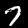
\includegraphics[width=0.1\columnwidth]{pics/MNIST/C7_4.png}
    & 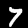
\includegraphics[width=0.1\columnwidth]{pics/MNIST/C7_5.png} 
    & 
\includegraphics[width=0.1\columnwidth]{pics/MNIST/C7_6.png}
    \\ 
    \rotatebox{90}{$Y_{\cdot 9}$}    
    &  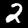
\includegraphics[width=0.1\columnwidth]{pics/MNIST/C9_1.png} 
    &  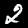
\includegraphics[width=0.1\columnwidth]{pics/MNIST/C9_2.png}
    &  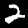
\includegraphics[width=0.1\columnwidth]{pics/MNIST/C9_3.png}
    & 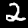
\includegraphics[width=0.1\columnwidth]{pics/MNIST/C9_4.png}
    & 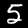
\includegraphics[width=0.1\columnwidth]{pics/MNIST/C9_5.png} 
    & 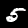
\includegraphics[width=0.1\columnwidth]{pics/MNIST/C9_6.png}
    \\ 
  \end{tabular}
  \caption{\textsc{SpectACl} clusters individual handwriting styles instead of cipher shapes.\label{fig:mnist}}
\end{figure}

%====================
% Discussion
%====================
\section{Discussion}
We introduce \textsc{SpectACl} (\emph{Spectral Averagely-dense Clustering}): a new clustering method that combines benefits from Spectral Clustering and the density-based DBSCAN algorithm, while avoiding some of their drawbacks. 

By computing the spectrum of the weighted adjacency matrix, \textsc{SpectACl} automatically determines the appropriate density for each cluster.  This eliminates the specification of the $minpts$ parameter which is required in DBSCAN, and as we have seen in Figure \ref{fig:intro}, this specification is a serious hurdle for a DBSCAN user to overcome. On two concentric circles with the same number of observations (and hence with different densities), a DBSCAN run with $minpts=25$ lumps all observations into one big cluster.  When increasing $minpts$ by one, DBSCAN jumps to four clusters, none of which are appropriate. \textsc{SpectACl}, conversely, can natively handle these nonconvex clusters with varying densities.

In both Spectral Clustering and \textsc{SpectACl}, the final step is to postprocess intermediate results with $k$-means. Whether this choice is appropriate for Spectral Clustering remains open to speculation.  However, from the objective function of \textsc{SpectACl}, we derive an upper bound through the eigenvector decomposition, whose optimization we show to be equal to $k$-means optimization.  Hence, for \textsc{SpectACl}, we demonstrate that this choice for $k$-means postprocessing is mathematically fundamentally sound.

In comparative experiments, competing with DBSCAN, Spectral Clustering, and Robust Spectral Clustering, we find on synthetic data that the unnormalized version of \textsc{SpectACl} is the most robust to noise (cf.\@ Figure~\ref{fig:noisePlot}), and finds the appropriate cluster structure in three scenarios while the competitors all fail to do so at least once (cf.\@ Figure~\ref{fig:synthViz}).  On real-life data, \textsc{SpectACl} outperforms the competition on the inherently noisy Pulsar dataset and the Sloan dataset, it performs similarly to Spectral Clustering on the SNAP dataset, and it is defeated by both Spectral Clustering and Robust Spectral Clustering on the MNIST dataset (cf.\@ Table~\ref{tbl:realNMI}). The latter observation is explained when looking at the resulting clusters: as Figure~\ref{fig:mnist} illustrates, \textsc{SpectACl} focuses on clusters representing handwriting style rather than clusters representing ciphers, which is not unreasonable behavior for an unsupervised method such as clustering; this uncovered information is merely not reflected in the NMI scores displayed in the table.

Figure~\ref{fig:paramPlot} provides evidence that \textsc{SpectACl} is robust with respect to its parameter settings.  Hence, in addition to its solid foundation in theory and good empirical performance on data, \textsc{SpectACl} provides a clustering method that is easy to use in practice.  Hence, \textsc{SpectACl} is an ideal candidate for outreach beyond data mining experts.
